\documentclass[letterpaper]{article}
\usepackage{makeidx}
\usepackage{natbib}
\usepackage{graphicx}
\usepackage{multicol}
\usepackage{float}
\usepackage{listings}
\usepackage{color}
\usepackage{ifthen}
\usepackage[table]{xcolor}
\usepackage{textcomp}
\usepackage{alltt}
\usepackage{ifpdf}
\ifpdf
\usepackage[pdftex,
            pagebackref=true,
            colorlinks=true,
            linkcolor=blue,
            unicode
           ]{hyperref}
\else
\usepackage[ps2pdf,
            pagebackref=true,
            colorlinks=true,
            linkcolor=blue,
            unicode
           ]{hyperref}
\usepackage{pspicture}
\fi
\usepackage[utf8]{inputenc}
\usepackage{mathptmx}
\usepackage[scaled=.90]{helvet}
\usepackage{courier}
\usepackage{sectsty}
\usepackage[titles]{tocloft}
\usepackage{doxygen}
\lstset{language=C++,inputencoding=utf8,basicstyle=\footnotesize,breaklines=true,breakatwhitespace=true,tabsize=3,numbers=left }
\makeindex
\setcounter{tocdepth}{3}
\renewcommand{\footrulewidth}{0.4pt}
\renewcommand{\familydefault}{\sfdefault}
\hfuzz=15pt
\setlength{\emergencystretch}{15pt}
\hbadness=750
\tolerance=750
\begin{document}
\hypersetup{pageanchor=false,citecolor=blue}
\begin{titlepage}
\vspace*{7cm}
\begin{center}
{\Large \-Allink \\[1ex]\large v0.\-1 }\\
\vspace*{1cm}
{\large \-Generated by Doxygen 1.7.6.1}\\
\vspace*{0.5cm}
{\small Thu Mar 27 2014 22:02:33}\\
\end{center}
\end{titlepage}
\pagenumbering{roman}
\tableofcontents
\pagenumbering{arabic}
\hypersetup{pageanchor=true,citecolor=blue}
\section{\-Allink}
\label{index}\hypertarget{index}{}\hypertarget{index_Overview_section}{}\subsection{\-Overview}\label{index_Overview_section}
\-Allink is a collection of analysis, visualisation and image processing tools to study the physical properties of the following systems\-: 
\begin{DoxyItemize}
\item \char`\"{}\-Bilayer membrane\char`\"{}\-: mechanical properties (bending, stretching and coupling energies, diffusivity, pressure tensor...). 
\item \char`\"{}\-Signals\char`\"{}\-: statistical properties (power spectrum, autocorrelation, distribution...). 
\item \char`\"{}\-Images\char`\"{}\-: statistical properties, filters, reconstruction of lines. 
\end{DoxyItemize}\-Allink is as well an integrator of equation of motion, \-Monte \-Carlo simulator and differential equation solver for the following systems\-: 
\begin{DoxyItemize}
\item \char`\"{}\-Integrator\char`\"{}\-: molecular dynamics for polymers, rotating rigid cylinders. 
\item \char`\"{}\-Simulator\char`\"{}\-: \-Monte \-Carlo with configurational bias for lipid systems. 
\item \char`\"{}\-Solver\char`\"{}\-: for a forth order differential equation in 1 or 2d lattices. 
\end{DoxyItemize}\-Each tools needs a configuration file inside the directory they are run to change the default options. \-This solution is preferred to the extensive use of menus which slows down the development of the software but makes the program less user friendly.\par
 \-Some tools are still under development if they are not properly documented. \par
 \-The programming style is modular, ojected oriented but not abstract (no use of friend classes, templates...). \-This might cause inefficiency in the program and in the source writing but is meant to furnish a clear understanding of the algorithms.\par
 \-The program is still under clean up of obsolete function and conversion of some original italian variable names. \paragraph*{\-Table of contents\-: }


\begin{DoxyItemize}
\item \-Avvis  
\item \hyperlink{ElPoly_page}{\-El\-Poly}  
\item \hyperlink{DrEffect_page}{\-Dr\-Effect}  
\item \-Addyn  
\end{DoxyItemize}\-Using \-Allink 
\begin{DoxyItemize}
\item \hyperlink{compile_page}{\-Compilation}  
\item \hyperlink{usage_page}{\-Getting \-Started}  
\item \hyperlink{param_page}{\-Parameter \-File} 
\item \hyperlink{design_page}{\-Design \-Overview}  
\end{DoxyItemize}\hyperlink{data_page}{\-Data \-Organization}   
\section{\-Dinamica}
\label{Dinamica_page}
\hypertarget{Dinamica_page}{}
Solution of a forth order differential equation on a lattice (solution of the Helfrich Hamiltonian). ~\newline
 The boundary condition are represented by the blue and red points, the minimum image convection can be applied or not in every direction.~\newline
 Optional\+:Open\+Gl. 
\begin{DoxyItemize}
\item \hyperlink{index}{Allink} (Up)  
\end{DoxyItemize}
\section{\-Visualizza}
\label{Visualizza_page}
\hypertarget{Visualizza_page}{}
Program for signal analysis\+:~\newline
 The programs loads a list of files assuming the first coordinate as x; the x and y coordinate can be changed with the right-\/up slider. ~\newline
 The lower left box choose the options for the visualisation (single set, log log, riscale...). ~\newline
 The lower sliders select the points for visualisation and analysis. The bottons on the rhs perform fittings, running average, distributions, integration... ~\newline
 Required\+:Qt4. 
\begin{DoxyItemize}
\item \hyperlink{index}{Allink} (Up)  
\end{DoxyItemize}
\section{\-Compilation}
\label{compile_page}
\hypertarget{compile_page}{}
\-Allink is written in \-A\-N\-S\-I standard \-C++, and must be compiled from source. \-It was developed using the gnu gcc compiler in both linux and \-Mac \-O\-S \-X environments. \-The source code should compile with any standards compliant \-C++ compiler. \-The build system, however, is based on \-Unix makefiles, and so will work only in a unix (linux or mac) environment.

\-Source code for the class library is in the src directory. \-Examples of main programs and example input files are in the \-Examples directory.\hypertarget{compile_page_compile_library_section}{}\subsection{\-Compile}\label{compile_page_compile_library_section}
\-To compile the entire \-Allink package 
\begin{DoxyItemize}
\item \-Edit /include/\-Make\-Include.mk and set the user defined flags. 
\item \-Run make.   
\end{DoxyItemize}

\-The resulting object $\ast$.o files for each class is placed in the same directory as the corresponding $\ast$.h and $\ast$.cpp source files. \-To clean up all of the $\ast$.o files and start over, enter \char`\"{}make clean\char`\"{} from the src directory.\hypertarget{compile_page_enable}{}\subsection{graphics}\label{compile_page_enable}
\hyperlink{classElPoly}{\-El\-Poly} has a visualisation tool if \-Open\-Gl libraries are installed. \hypertarget{compile_page_enable}{}\subsection{graphics}\label{compile_page_enable}
\hyperlink{classElPoly}{\-El\-Poly} uses for \-Delaunay triangulation the \-C\-G\-A\-L libraries.


\begin{DoxyItemize}
\item \hyperlink{index}{\-Allink} (\-Up)  
\item \hyperlink{usage_page}{\-Getting \-Started} (\-Next)  
\end{DoxyItemize}
\section{\-Extending \-Mol\-Mc\-D by \-Inheritance}
\label{extension_page}
\hypertarget{extension_page}{}
\-Mol\-Mc\-D defines several base classes that are intended to be extended by users. \-Among these are\-: 
\begin{DoxyItemize}
\item \-Species, which represents a molecular species.  
\item \-Md\-Integrator, which represents an \-M\-D integration algorithm. 
\item \-Mc\-Move, which represents a \-M\-C \-Markov move.  
\item \-Diagnostic, which represents a data analysis or output operation.  
\end{DoxyItemize}\-Users can add new features to the package by writing new subclasses of these base classes.

\-In order to fully integrate a user-\/defined subclass of any these base classes into \-Mol\-Mc\-D, one must also modify parts of the code that allow \-Mol\-Mc\-D to recognize and read the parameter file block associated with a new subclass. \-Once this is done, a user-\/defined subclass (e.\-g., a new \-Monte \-Carlo move) can be added to a simulation at run time using the same parameter file syntax as that used for subclasses that are distributed with the package.

\-The parameter file blocks associated with instances of these polymorphic base classes are all polymorphic blocks. \-The algorithm used by \-Mol\-Mc\-D to read a polymorphic block (i.\-e., a block which could refer to any of a known set of subclasses of a polymorphic base class) involves the use of a \-Factory class for each such base class. \-The \-Factory classes associated with the base classes listed above are called \-Species\-Factory, \-Md\-Integrator\-Factory, \-Mc\-Move\-Factory, \-Mc\-Diagnostic\-Factory (for diagnostics in \-M\-C simulations) and \-Md\-Diagnostic\-Factory (for \-M\-D simulations). \-The implementation of a \-Factory class defines a set of subclasses of the associated base class whose names and parameter file block formats will be recognized if they appear in the parameter file, so that they can thus be added to a simulation at run time. \-To integrate a new subclass of \-Species, \-Md\-Integrator, \-Mc\-Move or \-Diagnostic into \-Mol\-Mc\-D one must thus\-:


\begin{DoxyItemize}
\item \-Write the new subclass of the relevant base class.
\end{DoxyItemize}


\begin{DoxyItemize}
\item \-Extend the associated \-Factory class.
\end{DoxyItemize}


\begin{DoxyItemize}
\item \-Instruct an instance of the parent class to use a new customized \-Factory class when reading the parameter file.
\end{DoxyItemize}

\-Here, we provide instructions for steps (2) and (3), which are required to integrate a new subclass into \-Mol\-Mc\-D.\hypertarget{extension_page_factory_custom_sec}{}\subsection{\-Factory Classes}\label{extension_page_factory_custom_sec}
\-The \-Factory class associated with a class named \-Base (where base could be \-Mc\-Move, \-Diagnostic, etc.) is derived from the \-Factory $<$ \-Base $>$ class template. \-For example, \-Mc\-Move\-Factory is derived from the template \-Factory $<$ \-Mc\-Move $>$. \-The \-Factory class template declares a pure virtual method named factory(), which has the following interface. 
\begin{DoxyCode}
   template <class Base>
   Base* Factory<Base>::factory(std::string className) = 0;
\end{DoxyCode}
 \-This method take the name of a subclass of \-Base as a string parameter class\-Name. \-If it recognizes the name, it creates a new instance of the specified subclass, and returns a \-Base$\ast$ pointer to the new instance. \-The method should return a null pointer if it does not recognize the subclass name. \-The pointer to the new object can then be used by the invoking function to read the parameter file block associated with the new object, by invoking its read\-Param() method. \-In the default implementations of the \-Factory classes that are distributed with \-Mol\-Mc\-D, the factory method compares the classname string to the names of all of the subclasses of the relevant base class that are distributed with \-Mol\-Mc\-D, and creates a new instance of the desired subclass if it recognizes the name.

\-As an example, here is the segment of the file src/\-Md\-Integrator\-Factor.\-cpp that defines \-Md\-Integrator\-Factory\-::factory().


\begin{DoxyCode}
#include "MdIntegratorFactory.h"

// Subclasses of MdIntegrator 
#include "NVEIntegrator.h"
#include "NVTIntegrator.h"

namespace MolMcD 
{

   // Return a pointer to an new instance of an MdIntegrator subclass.
   MdIntegrator* MdIntegratorFactory::factory(std::string &className)
   {
      MdIntegrator *spp = 0;
      if (className == "NVEIntegrator") {
         spp = new NVEIntegrator(*systemPtr_);
      } else
      if (className == "NVTIntegrator") {
         spp = new NVTIntegrator(*systemPtr_);
      }
      return spp;
   }

}
\end{DoxyCode}
 \-If the string class\-Name matches the name \char`\"{}\-N\-V\-E\-Integrator\char`\"{} or \char`\"{}\-N\-V\-T\-Integrator\char`\"{}, the factory method will create a new instance of that subclass and returns a pointer to the new instance. \-Otherwise, if the string is not recognized, factory must return a null pointer, spp=0. \-The full source code for this class is in the files src/md\-Integrator/\-Md\-Integrator\-Factory.\-h and src/md\-Integrator/\-Md\-Integrator\-Factor.\-cpp.\hypertarget{extension_page_custom_factory_extend_sec}{}\subsection{\-Extending a Factory Class}\label{extension_page_custom_factory_extend_sec}
\-To extend the list of subclasses that can be recognized by a factory class, one can either\-: (1) \-Edit the default implementation that is provided with \-Mol\-Mc\-D, or (2) \-Define a subclass of the relevant \-Factory class, and re-\/implement that factory() method in the subclass. \-Despite the greater simplicity of the method (1), we recommend that users consider method (2) because it does not require the user to edit files that are provided with \-Mol\-Mc\-D, and thus allows the original files to remain synchronized with a revision control server and (if desired) shared by several users. \-We describe method (2) here.

\-As an example, imagine that you have written an \-N\-V\-T\-Langevin\-Integrator subclass of \-Md\-Integrator, , because no \-Langevin integrator is provided with the current version of the package. \-You should also define a subclass of \-Md\-Integrator\-Factory, which will be called \-My\-Md\-Integrator\-Factory, and re-\/implement the factory method. \-Here is an example of the required class definition\-: 
\begin{DoxyCode}
#include "MdIntegratorFactory.h"

// New user-defined subclass of MdIntegrator 
#include "LangevinNVTIntegrator.h"

namespace MolMcD 
{

   class MyMdIntegratorFactory : public MdIntegratorFactory 
   {

      MdIntegrator* factory(std::string &subclassName)
      {
         MdIntegrator *spp = 0;
         if (subclassName == "LangevinNVTIntegrator") {
            spp = new LangevinNVTIntegrator(*systemPtr_);
         } else {
            spp = MdIntegratorFactory::factory(subclassName);
         }
         return spp;
      }

   };

}
\end{DoxyCode}
 \-Note that the factory method first compares the class\-Name to the name \char`\"{}\-N\-V\-T\-Langevin\-Integrator\char`\"{}, but then passes class\-Name to the default factory method \-Md\-Integrator\-::factory() if class\-Name does not match \char`\"{}\-N\-V\-T\-Langevin\-Integrator\char`\"{}. \-The new method returns a null pointer (spp == 0) only if subclass\-Name does not match either \char`\"{}\-N\-V\-T\-Langevin\-Integrator\char`\"{} or any of the subclass names that are recognized by the default implementation.\hypertarget{extension_page_set_factory_extend_sec}{}\subsection{\-Registering a Custom Factory}\label{extension_page_set_factory_extend_sec}
\-After writing a new subclass of a base class and a subclass of the associated \-Factory, we must also instruct a parent class to use an instance of the user-\/defined \-Factory when reading the param file. \-This is done in the main program by creating an instance of the user defined \-Factory, and then invoking a \char`\"{}set\char`\"{} method of a parent object. \-The parent object is generally either the main \-Simulation object or a \-System object.

\-Below, we show an example of a main program for an \-Md\-Simulation that uses the subclass \-My\-Md\-Integrator\-Factory of \-Md\-Integrator\-Factory to read the \-Md\-Integrator block of a parameter file\-: 
\begin{DoxyCode}
namespace MolMcD
{

   int main 
   {
      McSimulation          sim;
      MyMdIntegratorFactory integratorFactory;
 
      \\ Register the custom Factory with the MdSystem
      sim.system().setMdIntegratorFactory(integratorFactory);

      \\ Read the parameter file from standard input
      sim.readParam(std::cin);
  
      \\ Run the simulation
      sim.run();
  
   }

}
\end{DoxyCode}
 \-In this example, \-The \-Md\-System\-::set\-Integrator\-Factory() method is invoked in order to register an instance of \-My\-Md\-Integrator\-Factory as the \-Md\-Integrator\-Factory that should be used by the \-Md\-System to read the block of the parameter file that contains a choice of integrator and the parameters required by the chosen integrator. \-In this example, the set\-Integrator\-Factory function is a method of \-Md\-System because an \-Md\-System has a pointer to an \-Md\-Integrator, and uses an \-Md\-Integrator\-Factory to read the associated sub-\/block of the parameter file.

\-If set\-Md\-Integrator\-Factory() is not called before \-Md\-Simulation\-::read\-Param, then \-Md\-System\-::read\-Param will automatically create and use an instance of \-Md\-Integrator\-Factory to read the \-Md\-Integrator block of the parameter file. \-The default implementation of \-Md\-Integrator\-Factory\-::factory() would then recognize only the subclasses of \-Md\-Integrator that are distributed with \-Mol\-Mc\-D.

\-A similar pattern is used to set user defined \-Factory classes for subclasses of \-Species, \-Mc\-Move, and \-Diagnostic, using set methods of of the relevant parent classes. \-Simulation class provides a set\-Species\-Factory() method, which can be used to set a new \-Species\-Factory in either \-M\-C or \-M\-D simulations. \-Mc\-Simulation provides a set\-Mc\-Move\-Factory() method. \-Mc\-Simulation and \-Md\-Simulation each provide a set\-Diagnostic\-Factory() method. \-In each case, if the set function is not invoked before the read\-Param() method of the parent object, then an instance of the default \-Factory class will be created and used to read the parameter file as needed.


\begin{DoxyItemize}
\item \hyperlink{param_page}{\-Parameter \-File} (\-Prevous)  
\item \hyperlink{index}{\-Allink} (\-Up)  
\item \hyperlink{typedef_page}{\-Potential \-Energy \-Typedefs} (\-Next)  
\end{DoxyItemize}
\section{\-Data \-Organization}
\label{data_page}
\hypertarget{data_page}{}

\begin{DoxyItemize}
\item \hyperlink{typedef_page}{\-Potential \-Energy \-Typedefs} (\-Previous)  
\item \hyperlink{index}{\-Allink} (\-Up)  
\end{DoxyItemize}
\section{\-Design \-Overview}
\label{design_page}
\hypertarget{design_page}{}

\begin{DoxyItemize}
\item \hyperlink{usage_page}{Getting Started} (Previous)  
\item \hyperlink{index}{Allink} (Up)  
\item \hyperlink{param_page}{Parameter File} (Next)  
\end{DoxyItemize}
\section{\-Dr\-Effect}
\label{DrEffect_page}
\hypertarget{DrEffect_page}{}
The programs perfom analysis on the loaded image and apply different user defined filters (convolution with Gaussian blur or discrete derivative, edge recognition and iterative construction...).~\newline
 Required\+:Open\+Gl Qt4.


\begin{DoxyItemize}
\item \hyperlink{index}{Allink} (Up)  
\end{DoxyItemize}
\section{\-El\-Poly}
\label{ElPoly_page}
\hypertarget{ElPoly_page}{}
\-Mechanical properties calculation for a system of particles bounded in chains. \par
 \-Perform a calculation of the characteristic properties of lipid chains in bilayer membrane (diffusivity, pressure profile, radial density plot...).\par
 \-Required\-:\-Open\-Gl, optional \-C\-G\-A\-L.\hypertarget{ElPoly_page_CommandList_section}{}\subsection{\-Command list\-:}\label{ElPoly_page_CommandList_section}
\-All the commands that can be typed in the command line can be written in the argument list with a single dash \char`\"{}-\/\char`\"{} for single characters or with double dash \char`\"{}-\/-\/\char`\"{} for words. 
\begin{DoxyItemize}
\item \char`\"{}dens\char`\"{} \hyperlink{classElPoly_a70302b7bbfa248d2963323bc63a4a292}{\-El\-Poly\-::\-Dens\-Prof} 
\item \char`\"{}3to2\char`\"{} \hyperlink{classElPoly_a4e71c4abd7c3ed37f29a8fcae064fd32}{\-El\-Poly\-::\-From3\-To2d} 
\item \char`\"{}3to1\char`\"{} \hyperlink{classElPoly_a0b9109dcecbeec17c94472b5e638580a}{\-El\-Poly\-::\-From3\-To1d} 
\item \char`\"{}2to1\char`\"{} \hyperlink{classElPoly_a30e6658740047a2fdd996e2b843e91b9}{\-El\-Poly\-::\-From2\-To1d} 
\item \char`\"{}pro\char`\"{} \hyperlink{classElPoly_aa2dbcd635807df0929968ec8932631ab}{\-El\-Poly\-::\-Projection\-F} 
\item \char`\"{}core\char`\"{} \hyperlink{classElPoly_a04dd79cb2f5e46ae301b6dc1d57db28a}{\-El\-Poly\-::\-Core\-F} 
\item \char`\"{}core\-Nano\char`\"{} \hyperlink{classElPoly_a04dd79cb2f5e46ae301b6dc1d57db28a}{\-El\-Poly\-::\-Core\-F} 
\item \char`\"{}\-Rad\-Shell\char`\"{} \hyperlink{classElPoly_a64e019ffaa4437477ea433f7b5113341}{\-El\-Poly\-::\-Radial\-Shell} 
\item \char`\"{}angle\char`\"{} \hyperlink{classElPoly_ae3aab8086f988eecdd12b8f29f45a56a}{\-El\-Poly\-::\-Angle} 
\item \char`\"{}\-Slab\-Prof\char`\"{} \hyperlink{classElPoly_a3db31f8490f0ea101281679a270e72fe}{\-El\-Poly\-::\-Slab\-Prof} 
\item \char`\"{}\-Slab\-Angle\-Profs\char`\"{} \hyperlink{classElPoly_a4192d526e79a4c1e0b4910a4f35720c4}{\-El\-Poly\-::\-Slab\-Angle\-Profs} 
\item \char`\"{}\-Cart\-Dens\char`\"{} \hyperlink{classElPoly_ac946a8b29f4eec0816699ce0c0cac23c}{\-El\-Poly\-::\-Cart\-Dens} 
\item \char`\"{}rad\-Nano\char`\"{} \hyperlink{classElPoly_aff852b942203d47f2e21e2616537cbdd}{\-El\-Poly\-::\-Rad\-Distr\-F} 
\item \char`\"{}rad\-Cm\char`\"{} \hyperlink{classElPoly_aff852b942203d47f2e21e2616537cbdd}{\-El\-Poly\-::\-Rad\-Distr\-F} 
\item \char`\"{}rad\-Cm\-N\char`\"{} \hyperlink{classElPoly_aff852b942203d47f2e21e2616537cbdd}{\-El\-Poly\-::\-Rad\-Distr\-F} 
\item \char`\"{}rad\-Stalk\char`\"{} \hyperlink{classElPoly_aff852b942203d47f2e21e2616537cbdd}{\-El\-Poly\-::\-Rad\-Distr\-F} 
\item \char`\"{}rad\-Pore\char`\"{} \hyperlink{classElPoly_aff852b942203d47f2e21e2616537cbdd}{\-El\-Poly\-::\-Rad\-Distr\-F} 
\item \char`\"{}cart\-Nano\char`\"{} \hyperlink{classElPoly_aff852b942203d47f2e21e2616537cbdd}{\-El\-Poly\-::\-Rad\-Distr\-F} 
\item \char`\"{}cm\char`\"{} \hyperlink{classElPoly_a59529de9a660df4734a218130963ae25}{\-El\-Poly\-::\-Center\-Of\-Mass} 
\item \char`\"{}\-Dens2\-Thick\char`\"{} \hyperlink{classElPoly_a7c40fb501bdadab09ee7cf8d99259299}{\-El\-Poly\-::\-Rad\-Dens2\-Thick} 
\item \char`\"{}\-Dens2\-Thick2d\char`\"{} \hyperlink{classElPoly_ad5ab39cdaa856caea3463819b436e7b9}{\-El\-Poly\-::\-Rad\-Dens2\-Thick2d} 
\item \char`\"{}\-Thick\-From\-Dens\char`\"{} \hyperlink{classElPoly_abcf175509352ac9dd90cb8ad96494219}{\-El\-Poly\-::\-Thick\-From\-Dens} 
\item \char`\"{}temp\char`\"{} \hyperlink{classElPoly_ad0651bcc7574507f16c1998b57822bdd}{\-El\-Poly\-::\-Temperature} 
\item \char`\"{}nano\char`\"{} \hyperlink{classElPoly_af9a89c5f8dc4c7274ec5e00ff4db78bb}{\-El\-Poly\-::\-Nano\-Particle} 
\item \char`\"{}surf\char`\"{} \hyperlink{classElPoly_a52844d3cee2d60eb47889fb021e10fc8}{\-El\-Poly\-::\-Surface} 
\item \char`\"{}diff\char`\"{} \hyperlink{classElPoly_a2f4aa8dc1e4dce0dc8fcb1d4b161757b}{\-El\-Poly\-::\-Diffusivity} 
\item \char`\"{}\-Diff\-Slab\char`\"{} \hyperlink{classElPoly_abf879a7d0b86a5eed8a5be87dc741200}{\-El\-Poly\-::\-Diff\-Slab} 
\item \char`\"{}\-Pair\-Corr\char`\"{} \hyperlink{classElPoly_a56b4b9780b4f84eb1713ca48b49fbbb2}{\-El\-Poly\-::\-Pair\-Corr} 
\item \char`\"{}pair\-Mon\char`\"{} \hyperlink{classElPoly_a7a3305d9ff38757faf367ced9abf89f0}{\-El\-Poly\-::\-Pair\-Correlation\-F} 
\item \char`\"{}pair\-Chain\char`\"{} \hyperlink{classElPoly_a7a3305d9ff38757faf367ced9abf89f0}{\-El\-Poly\-::\-Pair\-Correlation\-F} 
\item \char`\"{}pair\-Round\char`\"{} \hyperlink{classElPoly_a7a3305d9ff38757faf367ced9abf89f0}{\-El\-Poly\-::\-Pair\-Correlation\-F} 
\item \char`\"{}pair\-Square\char`\"{} \hyperlink{classElPoly_a7a3305d9ff38757faf367ced9abf89f0}{\-El\-Poly\-::\-Pair\-Correlation\-F} 
\item \char`\"{}pair\-Pep\char`\"{} \hyperlink{classElPoly_a7a3305d9ff38757faf367ced9abf89f0}{\-El\-Poly\-::\-Pair\-Correlation\-F} 
\item \char`\"{}\-Av\-Snap\char`\"{} \hyperlink{classElPoly_aafe33ef0f28995ba7c1a778196decf9b}{\-El\-Poly\-::\-Av\-Snap} 
\item \char`\"{}scatt\char`\"{} \hyperlink{classElPoly_a1aa4889418bf8c589875e1c77b5262d2}{\-El\-Poly\-::\-Scattering\-F} 
\item \char`\"{}scatt2\char`\"{} \hyperlink{classElPoly_a1aa4889418bf8c589875e1c77b5262d2}{\-El\-Poly\-::\-Scattering\-F} 
\item \char`\"{}worm\char`\"{} \hyperlink{classElPoly_ad6fa03abf69921d9a0759689569e35e9}{\-El\-Poly\-::\-Worm\-F} 
\item \char`\"{}header\char`\"{} \hyperlink{classElPoly_a2eab2da94941b822d51d4e21bfe64aef}{\-El\-Poly\-::\-Header\-Average} 
\item \char`\"{}spe\char`\"{} \hyperlink{classElPoly_ada953db0b772595339ef925b5dbd8c62}{\-El\-Poly\-::\-Spectrum\-F} 
\item \char`\"{}\-Rad\-Norm\-Pos\char`\"{} \hyperlink{classElPoly_ad3a244bc00c2c8216b1f5cbd36699cdc}{\-El\-Poly\-::\-Rad\-Norm\-Pos} 
\item \char`\"{}\-Area\-Distr\char`\"{} \hyperlink{classElPoly_a16d58960eae98f1ad67971068f12a22c}{\-El\-Poly\-::\-Area\-Distr\-F} 
\item \char`\"{}mid\char`\"{} \hyperlink{classElPoly_a16156b6e530ecc6df93b6ffd3c229f1b}{\-El\-Poly\-::\-Midplane} 
\item \char`\"{}mid\-Spe\char`\"{} \hyperlink{classElPoly_a669491e5e5c66f665694c9d8908d3109}{\-El\-Poly\-::\-Spectrum\-Midplane} 
\item \char`\"{}prop\char`\"{} \hyperlink{classElPoly_ae41ade7fbfd977babf42a7e2e6b33f07}{\-El\-Poly\-::\-Properties\-F} 
\item \char`\"{}div\-Opp\char`\"{} \hyperlink{classElPoly_acffadf1cdc641927dfd8af49eebc2069}{\-El\-Poly\-::\-Divide\-Layers} 
\item \char`\"{}div\-Tube\char`\"{} \hyperlink{classElPoly_acffadf1cdc641927dfd8af49eebc2069}{\-El\-Poly\-::\-Divide\-Layers} 
\item \char`\"{}div\-Ves\char`\"{} \hyperlink{classElPoly_acffadf1cdc641927dfd8af49eebc2069}{\-El\-Poly\-::\-Divide\-Layers} 
\item \char`\"{}\-Area\-Compr\char`\"{} \hyperlink{classElPoly_afbe805e551084aebeee2c673c9b3937a}{\-El\-Poly\-::\-Area\-Compr} 
\item \char`\"{}\-P\-Trace\char`\"{} \hyperlink{classElPoly_a534f27d79203f0b018acaedf41bbdb13}{\-El\-Poly\-::\-Press\-Trace} 
\item \char`\"{}\-P\-Radial\char`\"{} \hyperlink{classElPoly_a17a99c936b16e1880291e6c3c5957e44}{\-El\-Poly\-::\-Press\-Radial} 
\item \char`\"{}\-Tens\char`\"{} \hyperlink{classElPoly_af9a44196e456df096e96d914e19d85c9}{\-El\-Poly\-::\-Surf\-Tens} 
\item \char`\"{}\-Tens\-Cart\-Rad\char`\"{} \hyperlink{classElPoly_a7282d2e3fe0a3ee0caa631363913cc0a}{\-El\-Poly\-::\-Tens2d\-Cart\-Rad} 
\item \char`\"{}\-Sum\-Tens\char`\"{} \hyperlink{classElPoly_a35c812e3cfa8e0031dc2b521e075c1c9}{\-El\-Poly\-::\-Sum\-Tens} 
\item \char`\"{}stalk\char`\"{} \hyperlink{classElPoly_aba321cce3649252deca41a462b0e3d38}{\-El\-Poly\-::\-Stalk\-F} 
\item \char`\"{}\-Stalk\-Line\char`\"{} \hyperlink{classElPoly_adbfe7fc41363f770eee9c2a9e0e1ed57}{\-El\-Poly\-::\-Stalk\-Line\-Prof\-F} 
\item \char`\"{}\-Back\-Bone\char`\"{} \hyperlink{classVarData_abe9b658d50575d5d6be580bc87f3b4ac}{\-El\-Poly\-::\-Back\-Bone} 
\item \char`\"{}rem\char`\"{} \hyperlink{classElPoly_abfd537703af91a0dceb86c6bba5bd213}{\-El\-Poly\-::\-Remove\-Chains} 
\item \char`\"{}\-Ch\-Pos\char`\"{} 
\item \char`\"{}tra\char`\"{} \hyperlink{classVarData_aa63b2c1f38f3684a08db6394f92707f1}{\-El\-Poly\-::\-Transform} 
\item \char`\"{}\-Conv\-Lattice\char`\"{} \hyperlink{classElPoly_a3e03070150b93328661ff2c857eebbf4}{\-El\-Poly\-::\-Conv\-Lattice} 
\item \char`\"{}write\char`\"{} \hyperlink{classVarData_a054aab836dcf7735720ef32e0b8f7ecb}{\-El\-Poly\-::\-Write} 
\item \char`\"{}\-Widom\-Out\char`\"{} \hyperlink{classElPoly_aa7a92147aff6a466398908e0f92ca139}{\-El\-Poly\-::\-Widom\-Out} 
\item \char`\"{}\-Widom\-In\char`\"{} \hyperlink{classElPoly_a3e5c7ada1f6d5a2d37b23a9fb12771f9}{\-El\-Poly\-::\-Widom\-In} 
\item \char`\"{}\-End2\-End\char`\"{} \hyperlink{classElPoly_a15ee2b235143aabc133fe974aa3258a2}{\-El\-Poly\-::\-End2\-End\-Distr} 
\item \char`\"{}\-El\-Coup\char`\"{} \hyperlink{classElPoly_a48968ddc44376e55852e9720b3827ebe}{\-El\-Poly\-::\-Elastic\-Coupling} 
\item \char`\"{}\-El\-Coup\-N\-V\-T\char`\"{} \hyperlink{classElPoly_ab88192e9e4e0f11b68ad828d73ff8957}{\-El\-Poly\-::\-Elastic\-Coupling\-N\-V\-T} 
\item \char`\"{}\-E2\-E\-Dec\char`\"{} \hyperlink{classElPoly_a44e20767e332d941b94906f1a8e60e24}{\-El\-Poly\-::\-Decoupling} 
\item \char`\"{}\-Smooth\-Grid\char`\"{} \hyperlink{classVarData_a3d0e967c8f2515c16170245de47ffcbe}{\-El\-Poly\-::\-Smooth\-Grid} 
\item \char`\"{}\-Iso\-Surf\char`\"{} \hyperlink{classElPoly_a23b08e53b2acd3090051d2034632c20f}{\-El\-Poly\-::\-Iso\-Surf} 
\item \char`\"{}\-Iso\-Line\char`\"{} \hyperlink{classElPoly_a7af346569b401863e3d5f4541e85e0c4}{\-El\-Poly\-::\-Iso\-Line} 
\item \char`\"{}\-Iso\-Line\-Dens\char`\"{} \hyperlink{classElPoly_a7af346569b401863e3d5f4541e85e0c4}{\-El\-Poly\-::\-Iso\-Line} 
\item \char`\"{}\-F\-Pore\char`\"{} \hyperlink{classElPoly_aecd33584d71ae498798338253cbf83f0}{\-El\-Poly\-::\-Fetch\-Pore} 
\item \char`\"{}\-F\-Stalk\char`\"{} \hyperlink{classElPoly_a21a28de0471580af1978c3a48ae0ba0e}{\-El\-Poly\-::\-Fetch\-Stalk} 
\item \char`\"{}\-A\-Stalk\char`\"{} \hyperlink{classElPoly_a099625012512857cb5524bf15b397e5e}{\-El\-Poly\-::\-Stalk\-Area} 
\item \char`\"{}\-Shift2\-Center\char`\"{} \hyperlink{classElPoly_a2d5b51a7f120a4104f6e5070ca6c55f5}{\-El\-Poly\-::\-Shift2\-Center} 
\item \char`\"{}\-Av\-Snap\char`\"{} \hyperlink{classElPoly_aafe33ef0f28995ba7c1a778196decf9b}{\-El\-Poly\-::\-Av\-Snap} 
\item \char`\"{}\-Dir\-Dec\char`\"{} \hyperlink{classElPoly_a44e20767e332d941b94906f1a8e60e24}{\-El\-Poly\-::\-Decoupling} 
\item \char`\"{}\-Bil\-Dist\char`\"{} \hyperlink{classElPoly_a6f1477b110e5ee0e7e027466dac51b69}{\-El\-Poly\-::\-Bilayer\-Distance} 
\item \char`\"{}\-Bond\char`\"{} \hyperlink{classElPoly_a932a57ab32bd20f60bce8b498ca3095d}{\-El\-Poly\-::\-Bond\-Distr} 
\item \char`\"{}\-Diff2\-Dens\char`\"{} \hyperlink{classElPoly_a1c3688dd2704504d159802de5815643d}{\-El\-Poly\-::\-Diff2\-Files} 
\item \char`\"{}\-Diff2\-Pre\char`\"{} \hyperlink{classElPoly_a1c3688dd2704504d159802de5815643d}{\-El\-Poly\-::\-Diff2\-Files} 
\item \char`\"{}\-Rest\-Pre\char`\"{} \hyperlink{classElPoly_a019d255b1ff857ccd34550c7409a595b}{\-El\-Poly\-::\-Rest\-Press} 
\item \char`\"{}tecplot\-Dens\char`\"{} \hyperlink{classElPoly_ab03f8f580a4b45968aedcaa0d088c469}{\-El\-Poly\-::\-Conv2\-Tecplot} 
\item \char`\"{}tecplot\-Pre\char`\"{} \hyperlink{classElPoly_ab03f8f580a4b45968aedcaa0d088c469}{\-El\-Poly\-::\-Conv2\-Tecplot} 
\item \char`\"{}tecplot\-Hei\char`\"{} \hyperlink{classElPoly_ab03f8f580a4b45968aedcaa0d088c469}{\-El\-Poly\-::\-Conv2\-Tecplot} 
\item \char`\"{}rzd\char`\"{} \hyperlink{classElPoly_a538747fd3f643c9d171a00a5ec371ccc}{\-El\-Poly\-::\-Conv2rzd} 
\item \char`\"{}xyzd\char`\"{} \hyperlink{classElPoly_ad9aa947dfbb4fd8d4f2eb314efc17730}{\-El\-Poly\-::\-Conv2xyzd} 
\item \char`\"{}vmd\char`\"{} \hyperlink{classElPoly_a552193e7b9dea6d667fc1cd2ecab1482}{\-El\-Poly\-::\-Conv2\-Vmd} 
\item \char`\"{}povray\char`\"{} \hyperlink{classElPoly_ac2e836951a966bd69b21705cad363b95}{\-El\-Poly\-::\-Conv2\-Povray} 
\item \char`\"{}coord\char`\"{} 
\item \char`\"{}norm\char`\"{} 
\item \char`\"{}type\char`\"{} 
\item \char`\"{}file\char`\"{} \hyperlink{classElPoly_a5fa485410c0b7e02f523f96f33504435}{\-El\-Poly\-::\-Change\-File} 
\item \char`\"{}val\char`\"{} 
\item \char`\"{}\-Nei\char`\"{} \hyperlink{classVarData_ac99cf9cb839b06e0c3e32ebb8d11d6be}{\-El\-Poly\-::\-Find\-Neighbours} 
\item \char`\"{}sample\char`\"{} 
\item \char`\"{}open\char`\"{} \hyperlink{classElPoly_a3432306726a27b310ec27b3900894b11}{\-El\-Poly\-::\-Open\-File} 
\item \char`\"{}$>$\char`\"{} \hyperlink{classElPoly_a3432306726a27b310ec27b3900894b11}{\-El\-Poly\-::\-Open\-File} 
\item \char`\"{}$<$\char`\"{} \hyperlink{classElPoly_a3432306726a27b310ec27b3900894b11}{\-El\-Poly\-::\-Open\-File} 
\item \char`\"{}f\char`\"{} \hyperlink{classElPoly_a3432306726a27b310ec27b3900894b11}{\-El\-Poly\-::\-Open\-File} 
\item \char`\"{}info\char`\"{} \hyperlink{classVarData_a4dd85f1789027793b97a591acc9caf30}{\-El\-Poly\-::\-Sys\-Info} \hyperlink{classVarData_aa415b42b89dfba2ab8189be4e86b41ad}{\-El\-Poly\-::\-Sys\-Def} 
\item \char`\"{}q\char`\"{}


\end{DoxyItemize}


\begin{DoxyItemize}
\item \hyperlink{index}{\-Allink} (\-Up)  
\end{DoxyItemize}
\section{\-Current \-Features}
\label{features_page}
\hypertarget{features_page}{}
Mol\+McD is not yet a mature simulation package, but aspires to become one. The core of Mol\+McD was developed by rewriting a package named P\+MC that is used in our group for N\+VT simulations of coarse-\/grained bead-\/spring models of flexible polymer liquids. Both P\+MC and Mol\+McD thus far provide only the features that we have needed for these simulations. P\+MC provides several sophisticated conformation sampling MC moves for these simple models, which have not all yet been ported to Mol\+McD. Once all of the features of P\+MC are ported to Mol\+Mcd, further development work will focus on Mol\+McD. Features of Mol\+McD and P\+MC include\+: 
\begin{DoxyItemize}
\item Efficient implementations of N\+VE and N\+VT molecular dynamics, and hybrid M\+D/\+MC Markov moves. 


\item Configuration bias conformation sampling moves for MC simulation of dense liquids of long, flexible linear polymers. P\+MC provides crankshaft, reptation, end regrowth, internal rebrigding, and re-\/bridging configuration bias moves. Thus far, only reptation and end-\/regrowth moves have been ported to Mol\+McD. 


\item P\+MC implements \char`\"{}alchemical\char`\"{} moves for semigrand-\/canonical simulations of homopolymer mixtures, and end-\/swap moves for diblock copolymers. Neither has yet been ported to Mol\+McD. 


\item Specialized species definitions for isolated point particles, linear homopolymers, and diblock copolymers. 


\end{DoxyItemize}Thus far, the only potential energy classes provided with Mol\+McD are a simple LJ pair interaction and a harmonic bond potential. It does not yet support bending and dihedral potentials, or Coulomb interactions. We plan to add bond angle and dihedral potentials over the next few months, followed by Ewald and (later still) particle mesh Ewald implementations of electrostatic interactions.


\begin{DoxyItemize}
\item \hyperlink{index}{Allink} (Up)  
\item \hyperlink{compile_page}{Compilation} (Next)  
\end{DoxyItemize}
\section{\-Parameter \-File}
\label{param_page}
\hypertarget{param_page}{}
\hypertarget{usage_page_ElPoly_section}{}\subsection{\-El\-Poly}\label{usage_page_ElPoly_section}
\-Parameter file for the initialisation of a lipid system (used by \hyperlink{classElPoly}{\-El\-Poly})\-: 
\begin{DoxyCode}
#System:
IfSystem 0          #(0) .dat or (1) .xvl format files
#Soft: planar tube di6.0ibuted vesicle
NSoft 1             #number of soft bodies
#    Pos            Vel            Rad Hei Tens   type      name
#Soft x(0.5 0.5 0.5) v(0.0 0.0 0.0) c(3.0 0.0 1.0) s{vesicle} n{LIPID}
Soft x(0.5 0.5 0.5) v(0.0 0.0 0.0) c(6.0 0.0 1.0) s{planar} n{LIPID}
#Soft x(0.5 0.5 0.5) v(0.0 0.0 0.0) c(6.0 0.0 0.04) s{obstacle} n{LIPID}
#Soft x(0.5 0.5 0.7) v(0.0 0.0 0.0) c(6.0 0.0 1.0) s{planar} n{LIPID2}
#Soft x(0.5 0.5 0.3) v(0.0 0.0 0.0) c(6.0 0.0 1.0) s{planar} n{LIPID2}
Soft x(0.5 0.5 0.5) v(0.0 0.0 0.0) c(5.0 0.0 1.0) s{distributed} n{DISTR}
Soft x(0.5 0.5 0.5) v(0.0 0.0 0.0) c(5.0 0.0 1.5) s{coating} n{VESICLE}
Soft x(0.5 0.5 0.5) v(0.0 0.0 0.0) c(5.0 6.0 1.0) s{tube} n{LIPID}
#Geometry
Lx 12 Ly 12 Lz 14   #box size
CNorm  2            #normal direction
#Additional
NAddChain 0       #number of added chains
NStuffing 0         #number of phil monomers in the peptide
NSolvent  0000      #number of ghost solvent atoms
#Inclusion:
NNano 2            #number of nanoparticles
#     RelPos         Axis                rad  str  hei  coat
       [no,sph,cyl,wall,cluster,tilt,pore,dip]
#Rigid x(0.5 0.5 0.5) a(0.00 0.00 1.00) c(1.00 1.00 4.00 2.20) s{wall}
Rigid x(0.2 0.5 0.5) a(0.00 0.00 1.00) c(1.00 2.00 5.00 2.20) s{cluster}
Rigid x(0.7 0.5 0.5) a(0.00 0.00 1.00) c(1.00 2.00 5.00 2.20) s{cluster}
#Rigid x(0.5 0.5 0.57) a(1.00 0.00 0.00) c(.50 3.00 12.00 2.20) s{clinks}
#Rigid x(0.5 0.5 0.5) a(1.00 0.00 0.00) c(1.00 2.0 14.00 2.20) s{janus}
Rigid x(0.5 0.5 0.5) a(0.00 0.00 1.00) c(2.00 2000.00 6.00 2.20) s{cluster}
Rigid x(0.6 0.4 0.5) a(0.00 0.00 1.00) c(1.00 2000.00 6.00 2.20) s{cluster}
Rigid x(0.4 0.6 0.5) a(0.00 0.00 1.00) c(1.00 2000.00 6.00 2.20) s{cluster}
Rigid x(0.2 0.8 0.5) a(0.00 0.00 1.00) c(1.00 2000.00 6.00 2.20) s{cluster}

Rigid x(0.5 0.5 .9) a(0.00 0.00 1.00) c(1.0 0.5 2.00 0.0002) s{tip}
#Rigid x(0.5 0.5 .5) a(0.00 0.00 1.00) c(1.0 6.0 12.00 1.00) s{pore}
Rigid x(0.5 0.5 0.25) a(0.00 0.00 1.00) c(.5 1.0 4.00 1.00) s{wall}
Rigid x(0.5 0.5 0.5) a(0.00 0.00 1.00) c(2.0 2.0 6.00 2.20) s{cluster}
#Rigid x(0.5 0.5 0.5) a(0.00 0.00 1.00) c(1.0 6.0 14.00 1.00) s{sph}
Rigid x(0.5 0.5 0.5) a(0.00 0.00 1.00) c(1.00 6.00 10.00 2.20) s{tilt}
Rigid x(0.5 0.5 0.5) a(0.00 0.00 1.00) c(1.00 6.00 10.00 2.20) s{cyl}
NCircle 40        #number of monomer per 0.1ius unity
NHeight 5       #number of monomer per side unity
#Interactions:
chiN 30             #incompatibilty between the species
rho 10 6               #density coexistance
kappaN 70           #rigidity
kappaBend    3.     #bending coefficient
kappaSpring 20.537  #spring coefficient
ReOverCutOff 2      #Re/CutOff
vBB 0.1            #Chemical potential of the water
IfTwoTails 0        #construct the lipid with two tails
DiblockLim   8     #number of hydrophilic
NPartPChain  10   #number of beads per chain
WFuncStraight2 .9   #weighting function straight length
WFuncStraight3 1.   #weighting function straight length
\end{DoxyCode}
 \-Example of a system file\-: 
\begin{DoxyCode}
# L=12.000000 12.000000 18.000000 t=0.000000 blocks=2
# v=-24.33 -7.17 -24.33 0.10 -7.17 0.00 w=3.00 3.00 3.00 3.00 3.00 3.00 0.00
       3.00 3.00 0.00
# a2=0.9 a3=1.0 Re=2.0 N=10 ks=20.537 kb=3.000 l0=0
# Rigid x(6.00 6.00 9.00) a(0.00 0.00 1.00) c(1.00 1.00 4.00 2.2000) s{wall}
# Rigid x(2.40 2.40 3.60) a(0.00 0.00 1.00) c(1.00 1.00 4.00 2.2000) s{cyl}
# Pep x(6.00 6.00 9.00) a(0.00 0.00 1.00) g(2.00 6.00 2000.00) i[2] d[80 30]
       fn{Architecture2.dat}
# n=510 N=10 name=LIPID0
11.601412 10.858886 7.173472 0.158991 0.248636 -0.262377  0 
11.640605 11.011927 7.639597 0.171554 0.508449 0.081183  0 
11.558340 11.027104 7.401688 0.074257 0.331909 -0.188259  0 
11.366910 11.415070 7.646884 -0.261508 0.044753 0.115262  0 
11.287795 10.646103 7.537098 0.232126 0.155637 0.120164  0 
10.660425 10.121575 7.553806 -0.321680 0.239232 0.111970  0 
11.034412 10.219047 7.355556 -0.065595 0.134239 0.304619  0 
10.496886 9.737709 7.116385 -0.054618 0.079027 0.161831  0 
10.134289 9.152025 7.000000 -0.007443 0.177523 -0.165724  1 
10.234959 9.188418 6.805128 -0.101392 -0.369108 0.386933  1 
...
\end{DoxyCode}
 \-The same system in an alternative file format\-: 
\begin{DoxyCode}
# l( 12 12 18) c[511] s[0] n[7500] L[6] v[200] d[part] D(0.010000) i(6.00 30.00
       70.00) 
# Rigid x(6.00 6.00 9.00) a(0.00 0.00 1.00) c(1.00 1.00 4.00 2.2000) s{wall}
# Rigid x(2.40 2.40 3.60) a(0.00 0.00 1.00) c(1.00 1.00 4.00 2.2000) s{cyl}
# Pep x(6.00 6.00 9.00) a(0.00 0.00 1.00) g(2.00 6.00 2000.00) i[2] d[80 30]
       fn{Architecture2.dat}
{ t[0 0 0] x(1.189071 6.622403 7.549680) v(-0.176953 -0.431976 -0.035858) l[1] 
      }
{ t[1 0 0] x(1.139056 7.032122 7.560085) v(0.081602 0.258855 -0.281085) l[0] l[
      2] }
{ t[2 0 0] x(1.308140 6.519256 7.442227) v(-0.091691 -0.026668 -0.192819) l[1] 
      l[3] }
{ t[3 0 0] x(1.950485 6.142468 7.036736) v(-0.305010 0.196748 -0.057231) l[2] l
      [4] }
{ t[4 0 0] x(2.769803 5.534333 7.507009) v(-0.095458 -0.132241 0.174891) l[3] l
      [5] }
{ t[5 0 0] x(3.094308 5.454964 7.893810) v(0.301184 -0.342642 0.262871) l[4] l[
      6] }
{ t[6 0 0] x(2.911270 5.487582 7.605564) v(0.021949 0.001945 -0.102675) l[5] l[
      7] }
{ t[7 0 0] x(2.908146 5.974122 7.503403) v(0.095940 -0.258329 -0.459624) l[6] l
      [8] }
{ t[8 0 1] x(3.164008 6.124001 7.000000) v(-0.070202 -0.203646 0.363292) l[7] l
      [9] }
{ t[9 0 1] x(3.663501 5.760973 6.877247) v(-0.163645 0.152836 -0.317551) l[8] }
...
\end{DoxyCode}
\hypertarget{param_page_Draw_section}{}\subsection{\-Draw}\label{param_page_Draw_section}
\-Parameter file for the visualisation parameters (used by \hyperlink{classDraw}{\-Draw})\-: 
\begin{DoxyCode}
Pre           1                    #perspective
Passo         10                   #number of grid lines
Box           1                    #enable the box lines
OffSet        0. 0. 0.             #offset position
Rotate        -84. 0. 166.         #intial rotation
Sun           50. 1045. 0.         #sun position
Background    1. 1. 1.             #background color
Wheel         -1.35                #initial distance
GridEdge      0 0 0                #number of lines per edge
Legend        -.4 -.4 0. .4 .8     #position of the legend
Info          -.4 -.4 0.           #position of the info string
\end{DoxyCode}
 \-Example of a script for the \hyperlink{classDraw}{\-Draw} engine\-: 
\begin{DoxyCode}
#everything is normalized to 1
Arrow
0.0 0.3 0.0 1.0 3.0
0.0 0.0 0.0 1.0 0.0 0.0
Text
height
0.0 0.0 0.0 1.0 3.0
1.1 0.0 -0.05
Polygon #Wall
0.4 0.1 0.1 1.0
0.0 0.0 0.125
1.0 0.0 0.125
1.0 1.0 0.125
0.0 1.0 0.125
Fog #color(3) alpha(1) \\ dens(1) type(1) from(1) boh(2) to(1)
0.0 1.0 0.0 1.0
1 0.35 0.0 0.0 0.0 0.125
\end{DoxyCode}
\hypertarget{usage_page_Dinamica_section}{}\subsection{\-Dinamica}\label{usage_page_Dinamica_section}
\-Parameter file for a molecuar dynamics simulation (used by \-Dinamica)\-: 
\begin{DoxyCode}
#Sys size/type
NEdge       300            #number of particle per edge/box
Edge        20 20 20       #box size
SysShape    md             #0d 2d 3d leaves trial rigid mc md
CalcMode    NVT            #ensemble: NVT NcVT mcVT mVT
Potential   LJ             #potential: LJ LJ39 Harmonic
PotentialMode DensFunc     #Pair DensFunc DensFuncCh
#Dyn quantities
Deltat      0.003          #integration delta t
NChemPotId   200.          #eq number of particles
ChemPotEx   0              #interaction energy
Viscosity   0.2            #viscosity parameter
Temp        1              #temperature
#Force parameters
El          -1 -1 1265     #elastic coupling
Lap         3              #laplacian prefactor
SLap        0.1            #square laplacian prefactor
Ext         0.             #external force 
LJ          8.5            #Lennard Jones prefactor
LJMin       1              #Lennard Jones minimum
CutOff      1              #cutoff distance
Cont        0.             #contact/friction coefficient
Elong       0.2 0.1 0.2    #rest distance for the armonic spring
#boundary
IncrDist    0.01           #increase the distance of the selected bead
ExtRad      .12            #radius of the inclusion
ExtHeight   .52            #height of the inclusion
ExtAngle    60.            #contact angle
ExtCenter   .09 .0 .5      #position of the center
#tension profile
TNSlab      60             #number of slabs
TNDim       3              #number of dimensions
TNComp      6              #number of components
TCalcMode   2d             #calculation mode
#visualisation
NOut        1000           #number of points for visualizing the splines
IfMovie     0              #if produces images of the snaphots
IfLine      0              #if draws the line
NUpdate     1000           #how many timesteps before redrawing
IfInterp    0              #if interpolates the points
\end{DoxyCode}
 \-Parameter file for a \-Monte \-Carlo simulation (used by \-Dinamica)\-: 
\begin{DoxyCode}
#Sys size/type
NEdge       300            #number of particle per edge/box
Edge        20 20 20       #box size
SysShape    mc             #0d 2d 3d leaves trial rigid mc md
CalcMode    mcVT           #ensemble: NVT NcVT mcVT mVT
Potential   LJ             #potential: LJ LJ39 Harmonic
PotentialMode DensFuncCh   #Pair DensFunc DensFuncCh
SimLimit    100000         #maximum number of timesteps
#Dyn quantities
Deltat      0.003          #integration delta t
NChemPotId  100.           #eq number of particles
ChemPotEx   10.5        #ext chem pot (more neg: del,less neg: add)
Viscosity   0.2            #viscosity parameter
Temp        1              #temperature
#Force parameters
El          -1 -1 1265     #elastic coupling
Lap         3              #laplacian prefactor
SLap        0.1            #square laplacian prefactor
Ext         0.             #external force 
LJ          8.5            #Lennard Jones prefactor
LJMin       1              #Lennard Jones minimum
CutOff      1              #cutoff distance
Cont        0.             #contact/friction coefficient
Elong       0.2 0.1 0.2    #rest distance for the armonic spring
#boundary
IncrDist    0.01           #increase the distance of the selected bead
ExtRad      .12            #radius of the inclusion
ExtHeight   .52            #height of the inclusion
ExtAngle    60.            #contact angle
ExtCenter   .09 .0 .5      #position of the center
#tension profile
TNSlab      60             #number of slabs
TNDim       3              #number of dimensions
TNComp      6              #number of components
TCalcMode   3d             #calculation mode
#visualisation
NSpline     1000           #number of points for visualizing the splines
IfMovie     0              #if produces images of the snaphots
IfLine      0              #if draws the line
NUpdate     100            #how many timesteps before redrawing
NWrite      10000           #how many timesteps before writing 
IfInterp    0              #if interpolates the points
\end{DoxyCode}
 \-Parameter file for the solution od a differential equation in 2d (used by \-Dinamica)\-: 
\begin{DoxyCode}
Sys size/type
NEdge       60            #number of particle per edge/box
Edge        30 30 5       #box size
SysShape    2d pore         #0d 2d 3d leaves trial rigid mc md
CalcMode    NVT            #ensemble: NVT NcVT mcVT mVT
Potential   LJ             #potential: LJ LJ39 Harmonic
PotentialMode DensFunc     #Pair DensFunc DensFuncCh
Thermostat no #Langevin
#Dyn quantities
Deltat      0.003          #integration delta t
Viscosity 0.2
ChemPotId   200.           #eq number of particles
ChemPotEx   0              #interaction energy
Temp        1              #temperature
#Force parameters
El          1 -1 10000      #elastic coupling
Lap         0.52              #laplacian prefactor
SLap        1             #square laplacian prefactor
Ext         0.             #external force 
LJ          8.5            #Lennard Jones prefactor
LJMin       1              #Lennard Jones minimum
CutOff      1              #cutoff distance
Cont        0.             #contact/friction coefficient
Elong       0.2 0.1 0.05    #rest distance for the armonic spring
#boundary
Rigid x(15. 15. 0.0) a(0.00 0.00 1.00) c(1.0 35.00 2.0 2.2000) s{cyl}
#Rigid x(0.7 0.25 0.5) a(0.00 0.00 1.00) c(0.05 35.00 0.4 2.2000) s{cyl}
Boundary 1 1 1 1 0 0       #boundary conditions on x0 x1 y0 y1 z0 z1
Periodic 1 1 1             #periodic image convention on x y z 
#tension profile
TNSlab      60             #number of slabs
TNDim       3              #number of dimensions
TNComp      6              #number of components
TCalcMode   3d             #calculation mode
#visualisation
NSplie      1000
NOut        1000           #number of points for visualizing the splines
IfMovie     0              #if produces images of the snaphots
IfLine      0              #if draws the line
NUpdate     1000           #how many timesteps before redrawing
IfInterp    0              #if interpolates the points
NWrite      2000           #how many timesteps before dumping a trajectory file
\end{DoxyCode}
\hypertarget{usage_page_Visualizza_section}{}\subsection{\-Visualizza}\label{usage_page_Visualizza_section}
\-Script file for the plotting options (used by \-Visualizza)\-: 
\begin{DoxyCode}
# α-a β-b γ-c δ-d ε-e ζ-f η-g θ-h ι-i κ-l λ-k μ-l ν-m ξ-n ο-o π-p ρ-q σ-r ς-r
       τ-s υ-t φ-u ψ-v ω-x χ-y  
# http://htmlhelp.com/reference/html40/entities/symbols.html
NGrid
6 6
#XBound
-90 10
#YBound
5 500
FontSize
32
RatioWidthHeight
1.3
DigPrecX
2 f
DigPrecY
2 f
#ViewportX
0.05
#ViewportY
0.05
LabelX
q<sup>2</sup> [&Delta;L<sup>-2</sup>]
LabelY
&lang;h<sup>2</sup>&rang;L<sup>2</sup> [k<sub>B</sub>T]
#Title
Tension Profile
#ScaleX
1.0     
#OffSetX
-9.9
#ScaleY
3.9
PosLegend
.05 .25 .9 .9
PosInterp
.5 .9 
Line
1 #number of line
0.7 0.0 0.4 1.0 #color
2 # 0 no line, 1 dots, 2 lines, 3 lines and dots
midplane
Line
2 #number of line
0.0 0.7 0.0 1.0 #color
2 # 0 no line, 1 dots, 2 lines, 3 lines and dots
upper 
Line
3 #number of line
0.0 0.0 0.7 1.0 #color
2 # 0 no line, 1 dots, 2 lines, 3 lines and dots
lower
Line
4 #number of line
0.5 0.2 0.7 1.0 #color
2 # 0 no line, 1 dots, 2 lines, 3 lines and dots
thickness
PutStr
0. 0. 0. 1.
.17 .84 0 16
S 1 H 4
\end{DoxyCode}



\begin{DoxyItemize}
\item \hyperlink{index}{\-Allink} (\-Up)  
\item \hyperlink{design_page}{\-Design \-Overview} (\-Next)  
\end{DoxyItemize}
\section{\-Potential \-Energy \-Typedefs}
\label{typedef_page}
\hypertarget{typedef_page}{}
The potential energy functions used by M\+O\+L\+M\+CD cannot be chosen at run time, but can be easily modified at compile time, by redefining typedefs and recompiling. The potential energy classes used by Mol\+McD are referred to throughout the class library by a set of typedefs. Thus, for example, the class that represents a pair potential is referred to throughout the implementation of Md\+System and Mc\+System by a typedef \char`\"{}\+Pair\+Potential\char`\"{}. In the default configuration of Mol\+McD, \char`\"{}\+Pair\+Potential\char`\"{} is defined to be an alias for the \char`\"{}\+L\+J\+Potential\char`\"{} class.

In order to replace the Lennard-\/\+Jones potential by some other functional form for the pair potential, one must modify the typedef \char`\"{}\+Pair\+Potential\char`\"{} to refer to another pair potential class with the same interface, and then recompile the class library. The relevant typedefs for pair and bond potentials are defined in the header files src/base/\+Pair\+Potential.\+h and src/base/\+Bond\+Potential.\+h, respectively. Each of these typedef definition files also includes a header files for the actual pair and bond potential classes (e.\+g., L\+J\+Pair and Harmonic\+Bond), so that only class that includes the typedef also includes the header for the class to which it refers. See the documentation for these typedefs for a more detailed explanation of how to change potential classes by changing a few lines in the appropriate header.

We have chosen to use typedefs rather than polymorphic classes and virtual functions for the potential classes for reasons of efficiency. The force and energy evaluation methods are called repeatedly in the inner loops of MD and MC simulations, respectively. For efficiency, we would like to be able to inline these methods. The use of polymorphic classes with virtual force and energy evaluation methods would be more flexible, and would allow the user to choose potential energies at run time, without recompiling. It would also prevent inlining, however, and so would incur the full overhead associated with virtual function calls in the inner loop of either type of simulation.

The other candidate for similar treatment is the Boundary class. Boundary provides inline methods to evaluate separations and distances that are called within the inlined force and energy evaluation methods. At the moment, there is no need for a typedef because we have implemented only one version of the Boundary class, which represents a periodic orthorhombic unit cell. If and when we need the flexibility to define (for example) a more general triclinic unit cell, Boundary may be converted to a typedef in order to allow the user to select between orthorthombic and triclinic unit cells at compile time, while still allowing these functions to be inlined. 
\begin{DoxyItemize}
\item \hyperlink{extension_page}{Extending Mol\+McD by Inheritance} (Previous)  
\item \hyperlink{index}{Allink} (Up)  
\item \hyperlink{data_page}{Data Organization} (Next)  
\end{DoxyItemize}
\section{\-Getting \-Started}
\label{usage_page}
\hypertarget{usage_page}{}
\hypertarget{usage_page_ElPoly_section}{}\subsection{El\+Poly}\label{usage_page_ElPoly_section}
Create an intial system\+: edit Polymers.\+conf in the same directory and run 
\begin{DoxyCode}
\hyperlink{namespaceElPoly}{ElPoly} -x resume.dat
\end{DoxyCode}
 Study the properties of a system\+: 
\begin{DoxyCode}
\hyperlink{namespaceElPoly}{ElPoly} resume.dat
\end{DoxyCode}
 The option can be either specified in the argument list with a dash in the front 
\begin{DoxyCode}
\hyperlink{namespaceElPoly}{ElPoly} resume.dat -d part
\end{DoxyCode}
 or in the command line\+: 
\begin{DoxyCode}
[marelli@Hoshi]-(Examples) $ \hyperlink{namespaceElPoly}{ElPoly} resume.dat 
------------------------------------------------------
# NPart 7500 NType 0 NChain 511 NPCh 2410 Asymmetry 7499 Edge: [12 12 18] rho 6 chiN 30 kappaN 70 
Nano 64 (# 4) (1.000000 1.000000 4.000000) NBlock 1 NFile 1
\textcolor{preprocessor}{# SysType) Edge 1 Sys (Txvl 1 Xvt 0) }

------------------------------------------------------
\hyperlink{namespaceElPoly}{ElPoly}> 
\end{DoxyCode}
\hypertarget{usage_page_Visualizza_section}{}\subsection{Visualizza}\label{usage_page_Visualizza_section}
Run Visualizza specifing the argument list and the config file with \char`\"{}-\/c\char`\"{} 
\begin{DoxyCode}
Visualizza SpectrumBilayer*.dat FittedData*.dat -c PlotDef.txt &
\end{DoxyCode}
\hypertarget{usage_page_UsaMatematica_section}{}\subsection{Usa\+Matematica}\label{usage_page_UsaMatematica_section}
The same analysis tools of Visualizza can be run by Usa\+Matematica specifing a command with the double dash in the front or typing the command in the command line\+: 
\begin{DoxyCode}
UsaMatematica -x 1 -y 2 --exec x/6 y/35.2  DistMinSepRaw.dat -o Temp.dat
UsaMatematica --smoothGauss Temp.dat -o DistMinSep.dat
\end{DoxyCode}
\hypertarget{usage_page_DrImage_section}{}\subsection{Dr\+Image}\label{usage_page_DrImage_section}
Movie effects applied on a .png image. In the following example we run a Lennard-\/\+Jones simulation using squares of pixel as particles. 
\begin{DoxyCode}
DrImage Picture.png -l
\end{DoxyCode}
\hypertarget{usage_page_DrEffect_section}{}\subsection{Dr\+Effect}\label{usage_page_DrEffect_section}
Load a picture to apply the different filters and picture analysis 
\begin{DoxyCode}
\hyperlink{classDrEffect}{DrEffect} Picture.tif
\end{DoxyCode}
\hypertarget{usage_page_Dinamica_section}{}\subsection{Dinamica}\label{usage_page_Dinamica_section}
Run a simulation on a specific system with a specific integrator\+: 
\begin{DoxyCode}
Dinamica -c DynMC.conf -i resume.dat -d 
\end{DoxyCode}
 The option can be either specified in the argument list with a dash in the front or in the command line\+: \char`\"{}-\/d\char`\"{} display, \char`\"{}-\/r\char`\"{} run, \char`\"{}-\/-\/\+Tens\char`\"{} tension profile, \char`\"{}-\/-\/\+Av\+Forces\char`\"{} average forces...


\begin{DoxyItemize}
\item \hyperlink{compile_page}{Compilation} (Previous)  
\item \hyperlink{index}{Allink} (Up)  
\item \hyperlink{param_page}{Parameter File} (Next)  
\end{DoxyItemize}
\section{\-Directory \-Hierarchy}
\subsection{\-Directories}
\-This directory hierarchy is sorted roughly, but not completely, alphabetically\-:\begin{DoxyCompactList}
\item \contentsline{section}{include}{\pageref{dir_ba897815c9fce3fdfd715765e92e11b3}}{}
\item \contentsline{section}{src}{\pageref{dir_8e9a8b7e3c72bcc96dd64e909190dc02}}{}
\begin{DoxyCompactList}
\item \contentsline{section}{\-Addraw}{\pageref{dir_0282dfabc9d3d91e50dfe3859648f6c2}}{}
\item \contentsline{section}{\-Addyn}{\pageref{dir_9eb7b934b0b571f03e95a80abda3221c}}{}
\item \contentsline{section}{\-Avvis}{\pageref{dir_89df9d03b5edb33dc7a64ba8bbfbde4d}}{}
\item \contentsline{section}{\-Dr\-Effect}{\pageref{dir_d5ce84cef93befef5bda1b173f33bb3f}}{}
\item \contentsline{section}{\-El\-Poly}{\pageref{dir_1bb97581e94de66daf7acda7f0e3ec00}}{}
\item \contentsline{section}{\-Matematica}{\pageref{dir_d3aaf10f5e13657c742aaadcee9f6de1}}{}
\item \contentsline{section}{\-Segnali}{\pageref{dir_516fc008fde7d956e190d7ac2b4d9189}}{}
\item \contentsline{section}{\-Var\-Data}{\pageref{dir_4fd85bb7e60d3734b722333cda33b932}}{}
\end{DoxyCompactList}
\end{DoxyCompactList}

\section{\-Class \-Index}
\subsection{Class Hierarchy}
This inheritance list is sorted roughly, but not completely, alphabetically\+:\begin{DoxyCompactList}
\item \contentsline{section}{B\+L\+O\+CK}{\pageref{structBLOCK}}{}
\item \contentsline{section}{C\+H\+A\+IN}{\pageref{structCHAIN}}{}
\item \contentsline{section}{C\+I\+R\+C\+LE}{\pageref{structCIRCLE}}{}
\item \contentsline{section}{C\+O\+L\+OR}{\pageref{structCOLOR}}{}
\item \contentsline{section}{Dd\+Cell}{\pageref{structDdCell}}{}
\item \contentsline{section}{Dd\+Fix\+Cell}{\pageref{structDdFixCell}}{}
\item \contentsline{section}{D\+O\+M\+A\+I\+N\+\_\+\+P\+A\+RT}{\pageref{structDOMAIN__PART}}{}
\item \contentsline{section}{Dom\+Cell}{\pageref{classDomCell}}{}
\item \contentsline{section}{Dom\+Dec\+Basics}{\pageref{classDomDecBasics}}{}
\begin{DoxyCompactList}
\item \contentsline{section}{Dd\+Array}{\pageref{classDdArray}}{}
\item \contentsline{section}{Dd\+Double\+Loop}{\pageref{classDdDoubleLoop}}{}
\item \contentsline{section}{Dd\+Fixed\+Size}{\pageref{classDdFixedSize}}{}
\item \contentsline{section}{Dd\+Linked\+List}{\pageref{classDdLinkedList}}{}
\end{DoxyCompactList}
\item \contentsline{section}{Dom\+Part}{\pageref{classDomPart}}{}
\item \contentsline{section}{Draw}{\pageref{classDraw}}{}
\begin{DoxyCompactList}
\item \contentsline{section}{Dr\+Effect}{\pageref{classDrEffect}}{}
\end{DoxyCompactList}
\item \contentsline{section}{F\+O\+R\+C\+ES}{\pageref{structFORCES}}{}
\item \contentsline{section}{Funtore}{\pageref{classFuntore}}{}
\begin{DoxyCompactList}
\item \contentsline{section}{Spec\+Funtore$<$ Classe $>$}{\pageref{classSpecFuntore}}{}
\end{DoxyCompactList}
\item \contentsline{section}{G\+E\+N\+E\+R\+AL}{\pageref{structGENERAL}}{}
\item \contentsline{section}{G\+R\+I\+D\+C\+E\+LL}{\pageref{structGRIDCELL}}{}
\item \contentsline{section}{K\+F\+O\+R\+C\+ES}{\pageref{structKFORCES}}{}
\item \contentsline{section}{L\+I\+N\+KS}{\pageref{structLINKS}}{}
\item \contentsline{section}{Matematica}{\pageref{classMatematica}}{}
\begin{DoxyCompactList}
\item \contentsline{section}{Var\+Dat\+File}{\pageref{classVarDatFile}}{}
\item \contentsline{section}{Variabili}{\pageref{classVariabili}}{}
\end{DoxyCompactList}
\item \contentsline{section}{Mat\+Int}{\pageref{classMatInt}}{}
\item \contentsline{section}{Matrice}{\pageref{classMatrice}}{}
\item \contentsline{section}{M\+O\+M\+E\+N\+TI}{\pageref{structMOMENTI}}{}
\item \contentsline{section}{N\+A\+NO}{\pageref{structNANO}}{}
\item \contentsline{section}{Nei\+Vertex}{\pageref{classNeiVertex}}{}
\item \contentsline{section}{P\+A\+R\+A\+B\+O\+LA}{\pageref{structPARABOLA}}{}
\item \contentsline{section}{P\+A\+RT}{\pageref{structPART}}{}
\item \contentsline{section}{P\+E\+R\+M\+U\+TE}{\pageref{structPERMUTE}}{}
\item \contentsline{section}{Piano}{\pageref{classPiano}}{}
\item \contentsline{section}{Properties}{\pageref{classProperties}}{}
\item Q3\+V\+Box\begin{DoxyCompactList}
\item \contentsline{section}{Imposta\+N\+Bin}{\pageref{classImpostaNBin}}{}
\end{DoxyCompactList}
\item Q\+G\+L\+Widget\begin{DoxyCompactList}
\item \contentsline{section}{Animation}{\pageref{classAnimation}}{}
\end{DoxyCompactList}
\item \contentsline{section}{Q\+U\+A\+D\+RI}{\pageref{structQUADRI}}{}
\item \contentsline{section}{Quadri}{\pageref{classQuadri}}{}
\item \contentsline{section}{Quaternione}{\pageref{classQuaternione}}{}
\item Q\+Widget\begin{DoxyCompactList}
\item \contentsline{section}{Dr\+Finestra}{\pageref{classDrFinestra}}{}
\item \contentsline{section}{Dr\+Script}{\pageref{classDrScript}}{}
\item \contentsline{section}{Elementi\+Grafici}{\pageref{classElementiGrafici}}{}
\item \contentsline{section}{Finestra}{\pageref{classFinestra}}{}
\item \contentsline{section}{Finestra}{\pageref{classFinestra}}{}
\end{DoxyCompactList}
\item \contentsline{section}{R\+A\+D\+I\+CE}{\pageref{structRADICE}}{}
\item \contentsline{section}{R\+E\+T\+TA}{\pageref{structRETTA}}{}
\item \contentsline{section}{S\+E\+G\+N\+A\+LE}{\pageref{structSEGNALE}}{}
\item \contentsline{section}{Sing\+Proc}{\pageref{classSingProc}}{}
\item \contentsline{section}{S\+O\+FT}{\pageref{structSOFT}}{}
\item \contentsline{section}{Spline}{\pageref{classSpline}}{}
\item \contentsline{section}{S\+P\+L\+I\+NE}{\pageref{structSPLINE}}{}
\item \contentsline{section}{T\+E\+NS}{\pageref{structTENS}}{}
\item Triangulation\+\_\+face\+\_\+base\+\_\+2\begin{DoxyCompactList}
\item \contentsline{section}{My\+\_\+face\+\_\+base$<$ Gt $>$}{\pageref{classMy__face__base}}{}
\item \contentsline{section}{My\+\_\+face\+\_\+base$<$ Gt $>$}{\pageref{classMy__face__base}}{}
\item \contentsline{section}{My\+\_\+face\+\_\+base$<$ Gt $>$}{\pageref{classMy__face__base}}{}
\end{DoxyCompactList}
\item \contentsline{section}{V\+A\+R\+\_\+\+L\+I\+NE}{\pageref{structVAR__LINE}}{}
\item \contentsline{section}{V\+A\+R\+\_\+\+T\+R\+I\+A\+N\+G\+LE}{\pageref{structVAR__TRIANGLE}}{}
\item \contentsline{section}{Var\+Data}{\pageref{classVarData}}{}
\begin{DoxyCompactList}
\item \contentsline{section}{El\+Poly}{\pageref{classElPoly}}{}
\item \contentsline{section}{Forces}{\pageref{classForces}}{}
\end{DoxyCompactList}
\item \contentsline{section}{V\+E\+R\+T\+EX}{\pageref{structVERTEX}}{}
\item \contentsline{section}{V\+E\+TT}{\pageref{structVETT}}{}
\item \contentsline{section}{Vettore}{\pageref{classVettore}}{}
\item \contentsline{section}{X\+YZ}{\pageref{structXYZ}}{}
\end{DoxyCompactList}

\section{\-Class \-Index}
\subsection{\-Class \-List}
\-Here are the classes, structs, unions and interfaces with brief descriptions\-:\begin{DoxyCompactList}
\item\contentsline{section}{\hyperlink{classAnimation}{\-Animation} }{\pageref{classAnimation}}{}
\item\contentsline{section}{\hyperlink{structBLOCK}{\-B\-L\-O\-C\-K} \\*\-Information for every block }{\pageref{structBLOCK}}{}
\item\contentsline{section}{\hyperlink{structCHAIN}{\-C\-H\-A\-I\-N} \\*\-Information of every chain }{\pageref{structCHAIN}}{}
\item\contentsline{section}{\hyperlink{structCIRCLE}{\-C\-I\-R\-C\-L\-E} \\*\-Radius and center of a circle }{\pageref{structCIRCLE}}{}
\item\contentsline{section}{\hyperlink{structCOLOR}{\-C\-O\-L\-O\-R} }{\pageref{structCOLOR}}{}
\item\contentsline{section}{\hyperlink{classDdArray}{\-Dd\-Array} \\*\-Domain decomposition using arrays }{\pageref{classDdArray}}{}
\item\contentsline{section}{\hyperlink{structDdCell}{\-Dd\-Cell} \\*\-The array of particles in every cell }{\pageref{structDdCell}}{}
\item\contentsline{section}{\hyperlink{classDdDoubleLoop}{\-Dd\-Double\-Loop} \\*\-Stupid double loop to check the other pair loops }{\pageref{classDdDoubleLoop}}{}
\item\contentsline{section}{\hyperlink{structDdFixCell}{\-Dd\-Fix\-Cell} \\*\-The array of particles in every cell }{\pageref{structDdFixCell}}{}
\item\contentsline{section}{\hyperlink{classDdFixedSize}{\-Dd\-Fixed\-Size} \\*\-Domain decomposition using arrays }{\pageref{classDdFixedSize}}{}
\item\contentsline{section}{\hyperlink{classDdLinkedList}{\-Dd\-Linked\-List} \\*\-Domain decomposition as pointer to linked particles }{\pageref{classDdLinkedList}}{}
\item\contentsline{section}{\hyperlink{structDOMAIN__PART}{\-D\-O\-M\-A\-I\-N\-\_\-\-P\-A\-R\-T} \\*\-The previuos and consecutive particle in the cell linked list }{\pageref{structDOMAIN__PART}}{}
\item\contentsline{section}{\hyperlink{classDomCell}{\-Dom\-Cell} \\*\-For every cube how many particles and which are the first and the last }{\pageref{classDomCell}}{}
\item\contentsline{section}{\hyperlink{classDomDecBasics}{\-Dom\-Dec\-Basics} \\*\-All the general functions shared among the different domain decomposition structures }{\pageref{classDomDecBasics}}{}
\item\contentsline{section}{\hyperlink{classDomPart}{\-Dom\-Part} \\*\-The previuos and consecutive particle in the cell linked list }{\pageref{classDomPart}}{}
\item\contentsline{section}{\hyperlink{classDraw}{\-Draw} \\*\hyperlink{classDraw}{\-Draw} provides the basic configuration of the open\-G\-L libraries used in every derived program }{\pageref{classDraw}}{}
\item\contentsline{section}{\hyperlink{classDrEffect}{\-Dr\-Effect} }{\pageref{classDrEffect}}{}
\item\contentsline{section}{\hyperlink{classDrFinestra}{\-Dr\-Finestra} }{\pageref{classDrFinestra}}{}
\item\contentsline{section}{\hyperlink{classDrScript}{\-Dr\-Script} }{\pageref{classDrScript}}{}
\item\contentsline{section}{\hyperlink{classElementiGrafici}{\-Elementi\-Grafici} \\*\-Contains the function to interacts with the data stored in \hyperlink{classVarDatFile}{\-Var\-Dat\-File} }{\pageref{classElementiGrafici}}{}
\item\contentsline{section}{\hyperlink{classElPoly}{\-El\-Poly} \\*\-Operates and visualizes the information in the \hyperlink{classVarData}{\-Var\-Data} class }{\pageref{classElPoly}}{}
\item\contentsline{section}{\hyperlink{classFinestra}{\-Finestra} \\*\-Defines a window }{\pageref{classFinestra}}{}
\item\contentsline{section}{\hyperlink{structFORCES}{\-F\-O\-R\-C\-E\-S} \\*\-Single contribution of the forces }{\pageref{structFORCES}}{}
\item\contentsline{section}{\hyperlink{classForces}{\-Forces} \\*\-This class performs the different steps to solve the equations of motion via molecular dynamics simulation, simple grancanonical simulation in \-Monte \-Carlo and solution of 1d differential equations }{\pageref{classForces}}{}
\item\contentsline{section}{\hyperlink{classFuntore}{\-Funtore} }{\pageref{classFuntore}}{}
\item\contentsline{section}{\hyperlink{structGENERAL}{\-G\-E\-N\-E\-R\-A\-L} \\*\-General information of the system }{\pageref{structGENERAL}}{}
\item\contentsline{section}{\hyperlink{structGRIDCELL}{\-G\-R\-I\-D\-C\-E\-L\-L} \\*\-All the vertex in a cell }{\pageref{structGRIDCELL}}{}
\item\contentsline{section}{\hyperlink{classImpostaNBin}{\-Imposta\-N\-Bin} \\*\-Homemade slider }{\pageref{classImpostaNBin}}{}
\item\contentsline{section}{\hyperlink{structKFORCES}{\-K\-F\-O\-R\-C\-E\-S} \\*\-Prefactors of the forces }{\pageref{structKFORCES}}{}
\item\contentsline{section}{\hyperlink{structLINKS}{\-L\-I\-N\-K\-S} \\*\-Structure with the links of the particles }{\pageref{structLINKS}}{}
\item\contentsline{section}{\hyperlink{classMatematica}{\-Matematica} \\*\-Implementation of useful algorythms }{\pageref{classMatematica}}{}
\item\contentsline{section}{\hyperlink{classMatInt}{\-Mat\-Int} \\*\-Energy contribution from the density functional hamiltonian }{\pageref{classMatInt}}{}
\item\contentsline{section}{\hyperlink{classMatrice}{\-Matrice} \\*\hyperlink{classMatrice}{\-Matrice} computes the algebric operations on matrices }{\pageref{classMatrice}}{}
\item\contentsline{section}{\hyperlink{structMOMENTI}{\-M\-O\-M\-E\-N\-T\-I} \\*\-Moments of a distribution }{\pageref{structMOMENTI}}{}
\item\contentsline{section}{\hyperlink{classMy__face__base}{\-My\-\_\-face\-\_\-base$<$ Gt $>$} }{\pageref{classMy__face__base}}{}
\item\contentsline{section}{\hyperlink{structNANO}{\-N\-A\-N\-O} \\*\-Information about the nanoparticle }{\pageref{structNANO}}{}
\item\contentsline{section}{\hyperlink{classNeiVertex}{\-Nei\-Vertex} \\*\-Connects the triangles by vertices }{\pageref{classNeiVertex}}{}
\item\contentsline{section}{\hyperlink{structPARABOLA}{\-P\-A\-R\-A\-B\-O\-L\-A} \\*\-Parabolas coefficients }{\pageref{structPARABOLA}}{}
\item\contentsline{section}{\hyperlink{structPART}{\-P\-A\-R\-T} \\*\-Information of every particle }{\pageref{structPART}}{}
\item\contentsline{section}{\hyperlink{structPERMUTE}{\-P\-E\-R\-M\-U\-T\-E} \\*\-Indices for the permutation }{\pageref{structPERMUTE}}{}
\item\contentsline{section}{\hyperlink{classPiano}{\-Piano} \\*\-Define a plane }{\pageref{classPiano}}{}
\item\contentsline{section}{\hyperlink{classProperties}{\-Properties} \\*\-Some calculated properties of the system }{\pageref{classProperties}}{}
\item\contentsline{section}{\hyperlink{structQUADRI}{\-Q\-U\-A\-D\-R\-I} \\*\-Four dimentional vector/quaternion }{\pageref{structQUADRI}}{}
\item\contentsline{section}{\hyperlink{classQuadri}{\-Quadri} \\*\-Quaternion class }{\pageref{classQuadri}}{}
\item\contentsline{section}{\hyperlink{classQuaternione}{\-Quaternione} \\*\-Quaternion operations }{\pageref{classQuaternione}}{}
\item\contentsline{section}{\hyperlink{structRADICE}{\-R\-A\-D\-I\-C\-E} \\*\-Where a root was searched }{\pageref{structRADICE}}{}
\item\contentsline{section}{\hyperlink{structRETTA}{\-R\-E\-T\-T\-A} \\*\-Linear interpolation }{\pageref{structRETTA}}{}
\item\contentsline{section}{\hyperlink{structSEGNALE}{\-S\-E\-G\-N\-A\-L\-E} }{\pageref{structSEGNALE}}{}
\item\contentsline{section}{\hyperlink{classSingProc}{\-Sing\-Proc} \\*\-Basics class to start a \-M\-P\-I grid }{\pageref{classSingProc}}{}
\item\contentsline{section}{\hyperlink{structSOFT}{\-S\-O\-F\-T} \\*\-Information for every soft object }{\pageref{structSOFT}}{}
\item\contentsline{section}{\hyperlink{classSpecFuntore}{\-Spec\-Funtore$<$ Classe $>$} }{\pageref{classSpecFuntore}}{}
\item\contentsline{section}{\hyperlink{structSPLINE}{\-S\-P\-L\-I\-N\-E} \\*\-Coefficient of a spline }{\pageref{structSPLINE}}{}
\item\contentsline{section}{\hyperlink{classSpline}{\-Spline} \\*\-Coeficients of a \-N order spline }{\pageref{classSpline}}{}
\item\contentsline{section}{\hyperlink{structTENS}{\-T\-E\-N\-S} \\*\-Spatial tensor profile }{\pageref{structTENS}}{}
\item\contentsline{section}{\hyperlink{structVAR__LINE}{\-V\-A\-R\-\_\-\-L\-I\-N\-E} \\*\-Define a triangle }{\pageref{structVAR__LINE}}{}
\item\contentsline{section}{\hyperlink{structVAR__TRIANGLE}{\-V\-A\-R\-\_\-\-T\-R\-I\-A\-N\-G\-L\-E} \\*\-Define a triangle }{\pageref{structVAR__TRIANGLE}}{}
\item\contentsline{section}{\hyperlink{classVarData}{\-Var\-Data} \\*\-Reads and elaborates a system of chains }{\pageref{classVarData}}{}
\item\contentsline{section}{\hyperlink{classVarDatFile}{\-Var\-Dat\-File} \\*\-Reads and stores a data file to be elaborated via \hyperlink{classMatematica}{\-Matematica} }{\pageref{classVarDatFile}}{}
\item\contentsline{section}{\hyperlink{classVariabili}{\-Variabili} }{\pageref{classVariabili}}{}
\item\contentsline{section}{\hyperlink{structVERTEX}{\-V\-E\-R\-T\-E\-X} }{\pageref{structVERTEX}}{}
\item\contentsline{section}{\hyperlink{structVETT}{\-V\-E\-T\-T} \\*\-Three dimentional vector }{\pageref{structVETT}}{}
\item\contentsline{section}{\hyperlink{classVettore}{\-Vettore} \\*\-Geometrical operations on vectors }{\pageref{classVettore}}{}
\item\contentsline{section}{\hyperlink{structXYZ}{\-X\-Y\-Z} \\*\-A \-Cartesian tern }{\pageref{structXYZ}}{}
\end{DoxyCompactList}

\section{\-Directory \-Documentation}
\hypertarget{dir_0282dfabc9d3d91e50dfe3859648f6c2}{\subsection{src/\-Addraw/ \-Directory \-Reference}
\label{dir_0282dfabc9d3d91e50dfe3859648f6c2}\index{src/\-Addraw/ Directory Reference@{src/\-Addraw/ Directory Reference}}
}
\subsubsection*{\-Files}
\begin{DoxyCompactItemize}
\item 
file {\bfseries \-Draw.\-cpp}
\item 
file {\bfseries \-Draw\-Control.\-cpp}
\item 
file {\bfseries \-Draw\-Definition.\-cpp}
\item 
file {\bfseries \-Draw\-File.\-cpp}
\item 
file {\bfseries \-Draw\-Scene.\-cpp}
\item 
file {\bfseries \-Dr\-Image.\-cpp}
\item 
file {\bfseries \-Dr\-Image.\-h}
\item 
file {\bfseries \-Prova\-Draw.\-cpp}
\item 
file {\bfseries \-Read\-Write\-Png.\-cpp}
\end{DoxyCompactItemize}

\hypertarget{dir_9eb7b934b0b571f03e95a80abda3221c}{\subsection{src/\-Addyn/ \-Directory \-Reference}
\label{dir_9eb7b934b0b571f03e95a80abda3221c}\index{src/\-Addyn/ Directory Reference@{src/\-Addyn/ Directory Reference}}
}
\subsubsection*{\-Files}
\begin{DoxyCompactItemize}
\item 
file {\bfseries \-Dinamica.\-cpp}
\item 
file {\bfseries \-Dinamica.\-h}
\item 
file {\bfseries \-Forces.\-cpp}
\item 
file {\bfseries \-Forces.\-h}
\item 
file {\bfseries \-Forces\-Boundary.\-cpp}
\item 
file {\bfseries \-Forces\-Calc\-Energies.\-cpp}
\item 
file {\bfseries \-Forces\-Create.\-cpp}
\item 
file {\bfseries \-Forces\-Draw.\-cpp}
\item 
file {\bfseries \-Forces\-Force\-Field.\-cpp}
\item 
file {\bfseries \-Forces\-Integration.\-cpp}
\item 
file {\bfseries \-Forces\-Loop.\-cpp}
\item 
file {\bfseries \-Forces\-Tens.\-cpp}
\end{DoxyCompactItemize}

\hypertarget{dir_89df9d03b5edb33dc7a64ba8bbfbde4d}{\subsection{src/\-Avvis/ \-Directory \-Reference}
\label{dir_89df9d03b5edb33dc7a64ba8bbfbde4d}\index{src/\-Avvis/ Directory Reference@{src/\-Avvis/ Directory Reference}}
}
\subsubsection*{\-Files}
\begin{DoxyCompactItemize}
\item 
file {\bfseries \-Elementi\-Grafici.\-cpp}
\item 
file {\bfseries \-Elementi\-Grafici.\-h}
\item 
file {\bfseries \-Elementi\-Grafici\-Comm.\-cpp}
\item 
file {\bfseries \-Elementi\-Grafici\-Dis.\-cpp}
\item 
file {\bfseries \-Elementi\-Grafici\-El.\-cpp}
\item 
file {\bfseries \-Finestra.\-cpp}
\item 
file {\bfseries main.\-cpp}
\item 
file {\bfseries moc\-\_\-\-Elementi\-Grafici.\-cpp}
\item 
file {\bfseries \-Visualizza.\-cpp}
\end{DoxyCompactItemize}

\hypertarget{dir_d5ce84cef93befef5bda1b173f33bb3f}{\subsection{src/\-Dr\-Effect/ \-Directory \-Reference}
\label{dir_d5ce84cef93befef5bda1b173f33bb3f}\index{src/\-Dr\-Effect/ Directory Reference@{src/\-Dr\-Effect/ Directory Reference}}
}
\subsubsection*{\-Files}
\begin{DoxyCompactItemize}
\item 
file {\bfseries \-Animation.\-cpp}
\item 
file {\bfseries \-Dr\-Definition.\-cpp}
\item 
file {\bfseries \-Dr\-Effect.\-cpp}
\item 
file {\bfseries \-Dr\-Effect.\-h}
\item 
file {\bfseries \-Dr\-Finestra.\-cpp}
\item 
file {\bfseries \-Dr\-Finestra.\-h}
\item 
file {\bfseries \-Dr\-Open\-G\-L.\-cpp}
\item 
file {\bfseries \-Dr\-Script.\-cpp}
\item 
file {\bfseries \-Dr\-Script.\-h}
\end{DoxyCompactItemize}

\hypertarget{dir_1bb97581e94de66daf7acda7f0e3ec00}{\subsection{src/\-El\-Poly/ \-Directory \-Reference}
\label{dir_1bb97581e94de66daf7acda7f0e3ec00}\index{src/\-El\-Poly/ Directory Reference@{src/\-El\-Poly/ Directory Reference}}
}
\subsubsection*{\-Files}
\begin{DoxyCompactItemize}
\item 
file {\bfseries \-El\-Poly.\-cpp}
\item 
file {\bfseries \-El\-Poly.\-h}
\item 
file {\bfseries \-El\-Poly\-Draw.\-cpp}
\item 
file {\bfseries \-El\-Poly\-Draw\-C\-G\-A\-L.\-cpp}
\item 
file {\bfseries \-El\-Poly\-Draw\-Control.\-cpp}
\item 
file {\bfseries \-El\-Poly\-Draw\-Def.\-cpp}
\item 
file {\bfseries \-El\-Poly\-Draw\-Skin\-C\-G\-A\-L.\-cpp}
\item 
file {\bfseries \-El\-Poly\-Draw\-Surf.\-cpp}
\item 
file {\bfseries \-El\-Poly\-Draw\-Surf.\-h}
\item 
file {\bfseries \-El\-Poly\-Draw\-Surf\-C\-G\-A\-L.\-cpp}
\item 
file {\bfseries \-El\-Poly\-Draw\-Surf\-March\-Cubes.\-cpp}
\item 
file {\bfseries \-El\-Poly\-Draw\-Triang\-C\-G\-A\-L.\-cpp}
\item 
file {\bfseries \-El\-Poly\-El.\-cpp}
\item 
file {\bfseries \-El\-Poly\-Measure.\-cpp}
\item 
file {\bfseries \-El\-Poly\-Output.\-cpp}
\item 
file {\bfseries \-El\-Poly\-Prof\-Dens.\-cpp}
\item 
file {\bfseries \-El\-Poly\-Profile.\-cpp}
\item 
file {\bfseries \-El\-Poly\-Prof\-Pre.\-cpp}
\item 
file {\bfseries \-El\-Poly\-Repr.\-cpp}
\item 
file {\bfseries skin\-\_\-surface\-\_\-writer.\-h}
\end{DoxyCompactItemize}

\hypertarget{dir_ba897815c9fce3fdfd715765e92e11b3}{\subsection{include/ \-Directory \-Reference}
\label{dir_ba897815c9fce3fdfd715765e92e11b3}\index{include/ Directory Reference@{include/ Directory Reference}}
}
\subsubsection*{\-Files}
\begin{DoxyCompactItemize}
\item 
file {\bfseries \-Cubo.\-h}
\item 
file {\bfseries \-Draw.\-h}
\item 
file {\bfseries \-Matematica.\-h}
\item 
file {\bfseries \-Matematica\-Matrix.\-h}
\item 
file {\bfseries \-Matematica\-Plane.\-h}
\item 
file {\bfseries \-Matematica\-Quadri.\-h}
\item 
file {\bfseries \-Matematica\-Struct.\-h}
\item 
file {\bfseries \-Matematica\-Vect.\-h}
\item 
file {\bfseries mt19937ar.\-h}
\item 
file {\bfseries randomlib.\-h}
\item 
file {\bfseries \-Sing\-Proc.\-h}
\item 
file {\bfseries \-Var\-Data.\-h}
\item 
file {\bfseries \-Var\-Dat\-File.\-h}
\end{DoxyCompactItemize}

\hypertarget{dir_d3aaf10f5e13657c742aaadcee9f6de1}{\subsection{src/\-Matematica/ \-Directory \-Reference}
\label{dir_d3aaf10f5e13657c742aaadcee9f6de1}\index{src/\-Matematica/ Directory Reference@{src/\-Matematica/ Directory Reference}}
}
\subsubsection*{\-Files}
\begin{DoxyCompactItemize}
\item 
file {\bfseries \-Marsenne.\-h}
\item 
file {\bfseries \-Matematica.\-cpp}
\item 
file {\bfseries \-Matematica\-Algebra.\-cpp}
\item 
file {\bfseries \-Matematica\-Char.\-cpp}
\item 
file {\bfseries \-Matematica\-Filter.\-cpp}
\item 
file {\bfseries \-Matematica\-Func.\-cpp}
\item 
file {\bfseries \-Matematica\-Interp.\-cpp}
\item 
file {\bfseries \-Matematica\-Plane.\-cpp}
\item 
file {\bfseries \-Matematica\-Quaternion.\-cpp}
\item 
file {\bfseries \-Matematica\-Sign.\-cpp}
\item 
file {\bfseries \-Matematica\-Vect.\-cpp}
\item 
file {\bfseries mt19937ar.\-cpp}
\end{DoxyCompactItemize}

\hypertarget{dir_516fc008fde7d956e190d7ac2b4d9189}{\subsection{src/\-Segnali/ \-Directory \-Reference}
\label{dir_516fc008fde7d956e190d7ac2b4d9189}\index{src/\-Segnali/ Directory Reference@{src/\-Segnali/ Directory Reference}}
}
\subsubsection*{\-Files}
\begin{DoxyCompactItemize}
\item 
file {\bfseries \-Segnali.\-cpp}
\item 
file {\bfseries \-Segnali.\-h}
\item 
file {\bfseries \-Var\-Segnali.\-cpp}
\item 
file {\bfseries \-Var\-Segnali.\-h}
\end{DoxyCompactItemize}

\hypertarget{dir_8e9a8b7e3c72bcc96dd64e909190dc02}{\subsection{src/ \-Directory \-Reference}
\label{dir_8e9a8b7e3c72bcc96dd64e909190dc02}\index{src/ Directory Reference@{src/ Directory Reference}}
}
\subsubsection*{\-Directories}
\begin{DoxyCompactItemize}
\item 
directory \hyperlink{dir_0282dfabc9d3d91e50dfe3859648f6c2}{\-Addraw}
\item 
directory \hyperlink{dir_9eb7b934b0b571f03e95a80abda3221c}{\-Addyn}
\item 
directory \hyperlink{dir_89df9d03b5edb33dc7a64ba8bbfbde4d}{\-Avvis}
\item 
directory \hyperlink{dir_d5ce84cef93befef5bda1b173f33bb3f}{\-Dr\-Effect}
\item 
directory \hyperlink{dir_1bb97581e94de66daf7acda7f0e3ec00}{\-El\-Poly}
\item 
directory \hyperlink{dir_d3aaf10f5e13657c742aaadcee9f6de1}{\-Matematica}
\item 
directory \hyperlink{dir_516fc008fde7d956e190d7ac2b4d9189}{\-Segnali}
\item 
directory \hyperlink{dir_4fd85bb7e60d3734b722333cda33b932}{\-Var\-Data}
\end{DoxyCompactItemize}

\hypertarget{dir_4fd85bb7e60d3734b722333cda33b932}{\subsection{src/\-Var\-Data/ \-Directory \-Reference}
\label{dir_4fd85bb7e60d3734b722333cda33b932}\index{src/\-Var\-Data/ Directory Reference@{src/\-Var\-Data/ Directory Reference}}
}
\subsubsection*{\-Files}
\begin{DoxyCompactItemize}
\item 
file {\bfseries \-Cubo.\-cpp}
\item 
file {\bfseries \-Cubo.\-mirror.\-cpp}
\item 
file {\bfseries \-Polymers.\-cpp}
\item 
file {\bfseries \-Usa\-Matematica.\-cpp}
\item 
file {\bfseries \-Var\-Data.\-cpp}
\item 
file {\bfseries \-Var\-Data\-Back\-Fold.\-cpp}
\item 
file {\bfseries \-Var\-Data\-C\-G\-A\-L.\-cpp}
\item 
file {\bfseries \-Var\-Data\-Comm.\-cpp}
\item 
file {\bfseries \-Var\-Data\-Contour.\-cpp}
\item 
file {\bfseries \-Var\-Data\-Create.\-cpp}
\item 
file {\bfseries \-Var\-Data\-El.\-cpp}
\item 
file {\bfseries \-Var\-Data\-Exp.\-cpp}
\item 
file {\bfseries \-Var\-Data\-Interp.\-cpp}
\item 
file {\bfseries \-Var\-Data\-March\-Cubes.\-cpp}
\item 
file {\bfseries \-Var\-Data\-Pos.\-cpp}
\item 
file {\bfseries \-Var\-Data\-Profile.\-cpp}
\item 
file {\bfseries \-Var\-Data\-Read.\-cpp}
\item 
file {\bfseries \-Var\-Data\-String.\-cpp}
\item 
file {\bfseries \-Var\-Data\-Write.\-cpp}
\item 
file {\bfseries \-Var\-Dat\-File.\-cpp}
\end{DoxyCompactItemize}

\section{\-Class \-Documentation}
\hypertarget{classAnimation}{\subsection{\-Animation \-Class \-Reference}
\label{classAnimation}\index{\-Animation@{\-Animation}}
}
\subsubsection*{\-Public \-Slots}
\begin{DoxyCompactItemize}
\item 
\hypertarget{classAnimation_a59cabf1708863e82bdfced18dc630e37}{void {\bfseries set\-X\-Rotation} (int angle)}\label{classAnimation_a59cabf1708863e82bdfced18dc630e37}

\item 
\hypertarget{classAnimation_a38ddca1c05cad19158b0a88b172e857a}{void {\bfseries set\-Y\-Rotation} (int angle)}\label{classAnimation_a38ddca1c05cad19158b0a88b172e857a}

\item 
\hypertarget{classAnimation_a6cb4ef9b53294acc68dd22f74cebfbe9}{void {\bfseries set\-Z\-Rotation} (int angle)}\label{classAnimation_a6cb4ef9b53294acc68dd22f74cebfbe9}

\item 
\hypertarget{classAnimation_aed7f5207ef3aa32ebbdb28c9a1c1d82d}{void {\bfseries \-Nome\-File} (const \-Q\-String \&)}\label{classAnimation_aed7f5207ef3aa32ebbdb28c9a1c1d82d}

\item 
\hypertarget{classAnimation_aa7e7b6d7ce17b45aadd239d2bece1f6d}{void {\bfseries \-Nome\-File} (char $\ast$\-Ext\-Name)}\label{classAnimation_aa7e7b6d7ce17b45aadd239d2bece1f6d}

\item 
\hypertarget{classAnimation_a5e53001785ff30ae485a113b9b8a0ddc}{void {\bfseries \-Open} ()}\label{classAnimation_a5e53001785ff30ae485a113b9b8a0ddc}

\item 
\hypertarget{classAnimation_aee20dab02a80806a138b0f4741666efc}{void {\bfseries \-Filter} ()}\label{classAnimation_aee20dab02a80806a138b0f4741666efc}

\item 
\hypertarget{classAnimation_a3cb309e22382e343f4bf452cef422d80}{void {\bfseries \-Motion} ()}\label{classAnimation_a3cb309e22382e343f4bf452cef422d80}

\item 
\hypertarget{classAnimation_aa3eca255b6be227d7d901cc2a72017a5}{void {\bfseries \-Run} ()}\label{classAnimation_aa3eca255b6be227d7d901cc2a72017a5}

\item 
\hypertarget{classAnimation_a1dae0e52922866d32eafdda781b4be67}{void {\bfseries \-Filter\-M\-C} ()}\label{classAnimation_a1dae0e52922866d32eafdda781b4be67}

\item 
\hypertarget{classAnimation_af32a9408cd16ba5674acd0ffd8252805}{void {\bfseries \-Imp\-Grana} (int \-Grana)}\label{classAnimation_af32a9408cd16ba5674acd0ffd8252805}

\item 
\hypertarget{classAnimation_a2caf464d1f96559f2e06304c2532ccef}{void {\bfseries \-Filter\-Coarse\-Grain} ()}\label{classAnimation_a2caf464d1f96559f2e06304c2532ccef}

\item 
\hypertarget{classAnimation_a4fb4b0a2adf9a91d60743594a5b984b1}{void {\bfseries \-Filter\-Increase} ()}\label{classAnimation_a4fb4b0a2adf9a91d60743594a5b984b1}

\item 
\hypertarget{classAnimation_a8a662724ae20d82b9aefcb53bc118601}{void {\bfseries \-Filter\-Contrast} ()}\label{classAnimation_a8a662724ae20d82b9aefcb53bc118601}

\item 
\hypertarget{classAnimation_a8121ce6dcaabd895864fcb398d61830a}{void {\bfseries \-Histo} ()}\label{classAnimation_a8121ce6dcaabd895864fcb398d61830a}

\item 
\hypertarget{classAnimation_a4ac7178d0dc54a6e3ef5baf06f7c0f6a}{void {\bfseries \-Nabla\-Phi} ()}\label{classAnimation_a4ac7178d0dc54a6e3ef5baf06f7c0f6a}

\item 
\hypertarget{classAnimation_af982d1688f2311db74fc3f30bcdb793c}{void {\bfseries \-Black\-White} ()}\label{classAnimation_af982d1688f2311db74fc3f30bcdb793c}

\item 
\hypertarget{classAnimation_a51c2411cd4e39a465f686c9168b1aea0}{void {\bfseries \-Binary} ()}\label{classAnimation_a51c2411cd4e39a465f686c9168b1aea0}

\item 
\hypertarget{classAnimation_a2e9b853ff5bf26445c31024c75d56c1b}{void {\bfseries \-Punta} ()}\label{classAnimation_a2e9b853ff5bf26445c31024c75d56c1b}

\item 
\hypertarget{classAnimation_a70532654904bf37033660923eec20d03}{void {\bfseries \-Incr\-Slide} ()}\label{classAnimation_a70532654904bf37033660923eec20d03}

\end{DoxyCompactItemize}
\subsubsection*{\-Signals}
\begin{DoxyCompactItemize}
\item 
\hypertarget{classAnimation_a3ee26aac8a2fcea79a6b38dd7a4cba61}{void {\bfseries x\-Rotation\-Changed} (int angle)}\label{classAnimation_a3ee26aac8a2fcea79a6b38dd7a4cba61}

\item 
\hypertarget{classAnimation_a4760c62adb71794ef669f948eee3c604}{void {\bfseries y\-Rotation\-Changed} (int angle)}\label{classAnimation_a4760c62adb71794ef669f948eee3c604}

\item 
\hypertarget{classAnimation_aa8aec849822061b211a8e67691e0ae99}{void {\bfseries z\-Rotation\-Changed} (int angle)}\label{classAnimation_aa8aec849822061b211a8e67691e0ae99}

\item 
\hypertarget{classAnimation_ae1a9c67660ed6bcfb9839b0045d0263e}{void {\bfseries \-Punta\-Coord} (\hyperlink{classVarDatFile}{\-Var\-Dat\-File} $\ast$v1)}\label{classAnimation_ae1a9c67660ed6bcfb9839b0045d0263e}

\item 
\hypertarget{classAnimation_acbc1cbd5edc8e0a08391a999add774e3}{void {\bfseries \-Punta\-Coord} (double $\ast$$\ast$, int, int, int)}\label{classAnimation_acbc1cbd5edc8e0a08391a999add774e3}

\end{DoxyCompactItemize}
\subsubsection*{\-Public \-Member \-Functions}
\begin{DoxyCompactItemize}
\item 
\hypertarget{classAnimation_afa9802d69e8367d4b6677a508aa2e2a3}{{\bfseries \-Animation} (\-Q\-Widget $\ast$parent)}\label{classAnimation_afa9802d69e8367d4b6677a508aa2e2a3}

\item 
\hypertarget{classAnimation_ac0790850f6751e5fe0f47d16d7f67255}{void {\bfseries \-Init\-Constant} ()}\label{classAnimation_ac0790850f6751e5fe0f47d16d7f67255}

\item 
\hypertarget{classAnimation_afdf1ca9e7afc3e7ec41b47fea4b3d80d}{void {\bfseries \-Menu} ()}\label{classAnimation_afdf1ca9e7afc3e7ec41b47fea4b3d80d}

\item 
\hypertarget{classAnimation_abd86c6f19dd760d1ed1dce36d290582d}{void {\bfseries \-Particle} ()}\label{classAnimation_abd86c6f19dd760d1ed1dce36d290582d}

\item 
\hypertarget{classAnimation_aef7ba2f69afb2d954545f64c7fe24b14}{void {\bfseries keyboard} (unsigned char key, int x, int y)}\label{classAnimation_aef7ba2f69afb2d954545f64c7fe24b14}

\end{DoxyCompactItemize}
\subsubsection*{\-Public \-Attributes}
\begin{DoxyCompactItemize}
\item 
\hypertarget{classAnimation_af8d0da3e35bb5e28aba9329efffbfb95}{\hyperlink{classVarDatFile}{\-Var\-Dat\-File} $\ast$ {\bfseries v1}}\label{classAnimation_af8d0da3e35bb5e28aba9329efffbfb95}

\item 
\hypertarget{classAnimation_a6bd842874c8ee75e7889fabdbb9f98b2}{double $\ast$$\ast$ {\bfseries st}}\label{classAnimation_a6bd842874c8ee75e7889fabdbb9f98b2}

\end{DoxyCompactItemize}
\subsubsection*{\-Protected \-Member \-Functions}
\begin{DoxyCompactItemize}
\item 
\hypertarget{classAnimation_a2d3d45239c78255c23a70ca558b4d4f1}{virtual void {\bfseries initialize\-G\-L} ()}\label{classAnimation_a2d3d45239c78255c23a70ca558b4d4f1}

\item 
\hypertarget{classAnimation_adc7aa19ed77af08ab367a6cb77d2c13c}{virtual void {\bfseries paint\-Event} (\-Q\-Paint\-Event(event))}\label{classAnimation_adc7aa19ed77af08ab367a6cb77d2c13c}

\item 
\hypertarget{classAnimation_ac5cbfafb28ef4c0474ae96437294f547}{virtual void {\bfseries paint\-G\-L} ()}\label{classAnimation_ac5cbfafb28ef4c0474ae96437294f547}

\item 
\hypertarget{classAnimation_a3efe88f982dbec7825725dd954991139}{virtual void {\bfseries resize\-G\-L} (int width, int height)}\label{classAnimation_a3efe88f982dbec7825725dd954991139}

\item 
\hypertarget{classAnimation_ad2272e344e46519f026cd02f419884f1}{void {\bfseries mouse\-Press\-Event} (\-Q\-Mouse\-Event $\ast$event)}\label{classAnimation_ad2272e344e46519f026cd02f419884f1}

\item 
\hypertarget{classAnimation_ae820c6a86f0a1908bf451f86db043489}{void {\bfseries mouse\-Move\-Event} (\-Q\-Mouse\-Event $\ast$event)}\label{classAnimation_ae820c6a86f0a1908bf451f86db043489}

\end{DoxyCompactItemize}


\subsubsection{\-Detailed \-Description}


\-Definition at line 76 of file \-Dr\-Effect.\-h.



\-The documentation for this class was generated from the following files\-:\begin{DoxyCompactItemize}
\item 
src/\-Dr\-Effect/\-Dr\-Effect.\-h\item 
src/\-Dr\-Effect/\-Animation.\-cpp\end{DoxyCompactItemize}

\hypertarget{structBLOCK}{}\subsection{B\+L\+O\+CK Struct Reference}
\label{structBLOCK}\index{B\+L\+O\+CK@{B\+L\+O\+CK}}


Information for every block.  




{\ttfamily \#include $<$Var\+Data.\+h$>$}

\subsubsection*{Public Attributes}
\begin{DoxyCompactItemize}
\item 
char \hyperlink{structBLOCK_a7b413349ba4d10cbeb9b09be7c471c9e}{Name} \mbox{[}60\mbox{]}\hypertarget{structBLOCK_a7b413349ba4d10cbeb9b09be7c471c9e}{}\label{structBLOCK_a7b413349ba4d10cbeb9b09be7c471c9e}

\begin{DoxyCompactList}\small\item\em B\+Lock name. \end{DoxyCompactList}\item 
int \hyperlink{structBLOCK_a521663d12899e0fefe0a182332a8573f}{N\+P\+Ch}\hypertarget{structBLOCK_a521663d12899e0fefe0a182332a8573f}{}\label{structBLOCK_a521663d12899e0fefe0a182332a8573f}

\begin{DoxyCompactList}\small\item\em \subsubsection*{particles per chain}\end{DoxyCompactList}\item 
int \hyperlink{structBLOCK_abdcc792391d8c5092471dff191de47f4}{N\+Part}\hypertarget{structBLOCK_abdcc792391d8c5092471dff191de47f4}{}\label{structBLOCK_abdcc792391d8c5092471dff191de47f4}

\begin{DoxyCompactList}\small\item\em \subsubsection*{particles}\end{DoxyCompactList}\item 
int \hyperlink{structBLOCK_aa49e4d7af0d71e79524ef6fb081707b5}{N\+Chain}\hypertarget{structBLOCK_aa49e4d7af0d71e79524ef6fb081707b5}{}\label{structBLOCK_aa49e4d7af0d71e79524ef6fb081707b5}

\begin{DoxyCompactList}\small\item\em \subsubsection*{chains}\end{DoxyCompactList}\item 
int \hyperlink{structBLOCK_a71d10413e52e4e5aa82ac5e6189afdd0}{Init\+Idx}\hypertarget{structBLOCK_a71d10413e52e4e5aa82ac5e6189afdd0}{}\label{structBLOCK_a71d10413e52e4e5aa82ac5e6189afdd0}

\begin{DoxyCompactList}\small\item\em Initial particle position. \end{DoxyCompactList}\item 
int \hyperlink{structBLOCK_a3fa6306dcea956ea84ce7b5f2b22f628}{End\+Idx}\hypertarget{structBLOCK_a3fa6306dcea956ea84ce7b5f2b22f628}{}\label{structBLOCK_a3fa6306dcea956ea84ce7b5f2b22f628}

\begin{DoxyCompactList}\small\item\em End particle position. \end{DoxyCompactList}\item 
int \hyperlink{structBLOCK_ab953dc37c933d1b21ba1d94b87c65bca}{Arch}\hypertarget{structBLOCK_ab953dc37c933d1b21ba1d94b87c65bca}{}\label{structBLOCK_ab953dc37c933d1b21ba1d94b87c65bca}

\begin{DoxyCompactList}\small\item\em Architecture type. \end{DoxyCompactList}\item 
int \hyperlink{structBLOCK_ad984dd2cb572ac6c2deac801d0c2f947}{n\+Nano}\hypertarget{structBLOCK_ad984dd2cb572ac6c2deac801d0c2f947}{}\label{structBLOCK_ad984dd2cb572ac6c2deac801d0c2f947}

\begin{DoxyCompactList}\small\item\em Nano index. \end{DoxyCompactList}\item 
int \hyperlink{structBLOCK_af914cf19bda574d081fa0a7b243bf7dc}{Asym}\hypertarget{structBLOCK_af914cf19bda574d081fa0a7b243bf7dc}{}\label{structBLOCK_af914cf19bda574d081fa0a7b243bf7dc}

\begin{DoxyCompactList}\small\item\em Diblock limit of the chain. \end{DoxyCompactList}\end{DoxyCompactItemize}


\subsubsection{Detailed Description}
Information for every block. 

Definition at line 255 of file Var\+Data.\+h.



The documentation for this struct was generated from the following file\+:\begin{DoxyCompactItemize}
\item 
include/Var\+Data.\+h\end{DoxyCompactItemize}

\hypertarget{structCHAIN}{\subsection{\-C\-H\-A\-I\-N \-Struct \-Reference}
\label{structCHAIN}\index{\-C\-H\-A\-I\-N@{\-C\-H\-A\-I\-N}}
}


\-Information of every chain.  




{\ttfamily \#include $<$\-Var\-Data.\-h$>$}

\subsubsection*{\-Public \-Attributes}
\begin{DoxyCompactItemize}
\item 
\hypertarget{structCHAIN_ac00d29ea47aa8845638961a34cb3ec0e}{double \hyperlink{structCHAIN_ac00d29ea47aa8845638961a34cb3ec0e}{\-Pos} \mbox{[}4\mbox{]}}\label{structCHAIN_ac00d29ea47aa8845638961a34cb3ec0e}

\begin{DoxyCompactList}\small\item\em xyzr \-Postion of the chain \end{DoxyCompactList}\item 
\hypertarget{structCHAIN_ac77c91979738079508cf3f257a7164ba}{double \hyperlink{structCHAIN_ac77c91979738079508cf3f257a7164ba}{\-Dir} \mbox{[}3\mbox{]}}\label{structCHAIN_ac77c91979738079508cf3f257a7164ba}

\begin{DoxyCompactList}\small\item\em \-Directive of the chain. \end{DoxyCompactList}\item 
\hypertarget{structCHAIN_ae3fae9edc78d8cadc33c5a52bebdb46c}{double \hyperlink{structCHAIN_ae3fae9edc78d8cadc33c5a52bebdb46c}{\-Vel} \mbox{[}3\mbox{]}}\label{structCHAIN_ae3fae9edc78d8cadc33c5a52bebdb46c}

\begin{DoxyCompactList}\small\item\em \-Chain velocity. \end{DoxyCompactList}\item 
\hypertarget{structCHAIN_a8c10230001bab42de01beb2843f8c327}{double {\bfseries \-Angle}}\label{structCHAIN_a8c10230001bab42de01beb2843f8c327}

\item 
\hypertarget{structCHAIN_ae011432eaca3858364b05a111f4011d3}{int \hyperlink{structCHAIN_ae011432eaca3858364b05a111f4011d3}{\-Type}}\label{structCHAIN_ae011432eaca3858364b05a111f4011d3}

\begin{DoxyCompactList}\small\item\em \-Type of the chain (see list \-C\-H\-A\-I\-N\-\_\-) \end{DoxyCompactList}\item 
\hypertarget{structCHAIN_a521663d12899e0fefe0a182332a8573f}{int \hyperlink{structCHAIN_a521663d12899e0fefe0a182332a8573f}{\-N\-P\-Ch}}\label{structCHAIN_a521663d12899e0fefe0a182332a8573f}

\begin{DoxyCompactList}\small\item\em \-Number of particles per chain. \end{DoxyCompactList}\item 
\hypertarget{structCHAIN_ae42336bc0bf033452fba9451cf1e9bc5}{int \hyperlink{structCHAIN_ae42336bc0bf033452fba9451cf1e9bc5}{\-Init\-Bead}}\label{structCHAIN_ae42336bc0bf033452fba9451cf1e9bc5}

\begin{DoxyCompactList}\small\item\em \-Initial bead. \end{DoxyCompactList}\item 
\hypertarget{structCHAIN_a3d5741424865c77e0404a26fe8d11b94}{int \hyperlink{structCHAIN_a3d5741424865c77e0404a26fe8d11b94}{\-End\-Bead}}\label{structCHAIN_a3d5741424865c77e0404a26fe8d11b94}

\begin{DoxyCompactList}\small\item\em \-End bead. \end{DoxyCompactList}\end{DoxyCompactItemize}


\subsubsection{\-Detailed \-Description}
\-Information of every chain. 

\-Definition at line 236 of file \-Var\-Data.\-h.



\-The documentation for this struct was generated from the following file\-:\begin{DoxyCompactItemize}
\item 
include/\-Var\-Data.\-h\end{DoxyCompactItemize}

\hypertarget{structCIRCLE}{}\subsection{C\+I\+R\+C\+LE Struct Reference}
\label{structCIRCLE}\index{C\+I\+R\+C\+LE@{C\+I\+R\+C\+LE}}


Radius and center of a circle.  




{\ttfamily \#include $<$Matematica\+Struct.\+h$>$}

\subsubsection*{Public Attributes}
\begin{DoxyCompactItemize}
\item 
double \hyperlink{structCIRCLE_a860bef50013f57ab1a6437b7986a9487}{Rad}\hypertarget{structCIRCLE_a860bef50013f57ab1a6437b7986a9487}{}\label{structCIRCLE_a860bef50013f57ab1a6437b7986a9487}

\begin{DoxyCompactList}\small\item\em Radius of the circle. \end{DoxyCompactList}\item 
double \hyperlink{structCIRCLE_a948efd29e2703858b2752cdba79b89c2}{xC}\hypertarget{structCIRCLE_a948efd29e2703858b2752cdba79b89c2}{}\label{structCIRCLE_a948efd29e2703858b2752cdba79b89c2}

\begin{DoxyCompactList}\small\item\em x position of the center \end{DoxyCompactList}\item 
double \hyperlink{structCIRCLE_a7d873dd60d81fee341939655db765355}{yC}\hypertarget{structCIRCLE_a7d873dd60d81fee341939655db765355}{}\label{structCIRCLE_a7d873dd60d81fee341939655db765355}

\begin{DoxyCompactList}\small\item\em y position of the center \end{DoxyCompactList}\end{DoxyCompactItemize}


\subsubsection{Detailed Description}
Radius and center of a circle. 

Definition at line 49 of file Matematica\+Struct.\+h.



The documentation for this struct was generated from the following file\+:\begin{DoxyCompactItemize}
\item 
include/Matematica\+Struct.\+h\end{DoxyCompactItemize}

\hypertarget{structCOLOR}{\subsection{\-C\-O\-L\-O\-R \-Struct \-Reference}
\label{structCOLOR}\index{\-C\-O\-L\-O\-R@{\-C\-O\-L\-O\-R}}
}
\subsubsection*{\-Public \-Attributes}
\begin{DoxyCompactItemize}
\item 
\hypertarget{structCOLOR_a880a49112fedae68e714341a9a082fb6}{double {\bfseries r}}\label{structCOLOR_a880a49112fedae68e714341a9a082fb6}

\item 
\hypertarget{structCOLOR_ab30c765b9be1b7776c97c899a12a66bb}{double {\bfseries g}}\label{structCOLOR_ab30c765b9be1b7776c97c899a12a66bb}

\item 
\hypertarget{structCOLOR_a1510a66dacf9cf3586de5fc89ae2a073}{double {\bfseries b}}\label{structCOLOR_a1510a66dacf9cf3586de5fc89ae2a073}

\item 
\hypertarget{structCOLOR_a1031d0e0a97a340abfe0a6ab9e831045}{double {\bfseries a}}\label{structCOLOR_a1031d0e0a97a340abfe0a6ab9e831045}

\end{DoxyCompactItemize}


\subsubsection{\-Detailed \-Description}


\-Definition at line 68 of file \-El\-Poly\-Draw\-C\-G\-A\-L.\-cpp.



\-The documentation for this struct was generated from the following files\-:\begin{DoxyCompactItemize}
\item 
src/\-El\-Poly/\-El\-Poly\-Draw\-C\-G\-A\-L.\-cpp\item 
src/\-El\-Poly/\-El\-Poly\-Draw\-Triang\-C\-G\-A\-L.\-cpp\end{DoxyCompactItemize}

\hypertarget{classDdArray}{}\subsection{Dd\+Array Class Reference}
\label{classDdArray}\index{Dd\+Array@{Dd\+Array}}


Domain decomposition using arrays.  




{\ttfamily \#include $<$Cubo.\+h$>$}

Inheritance diagram for Dd\+Array\+:\begin{figure}[H]
\begin{center}
\leavevmode
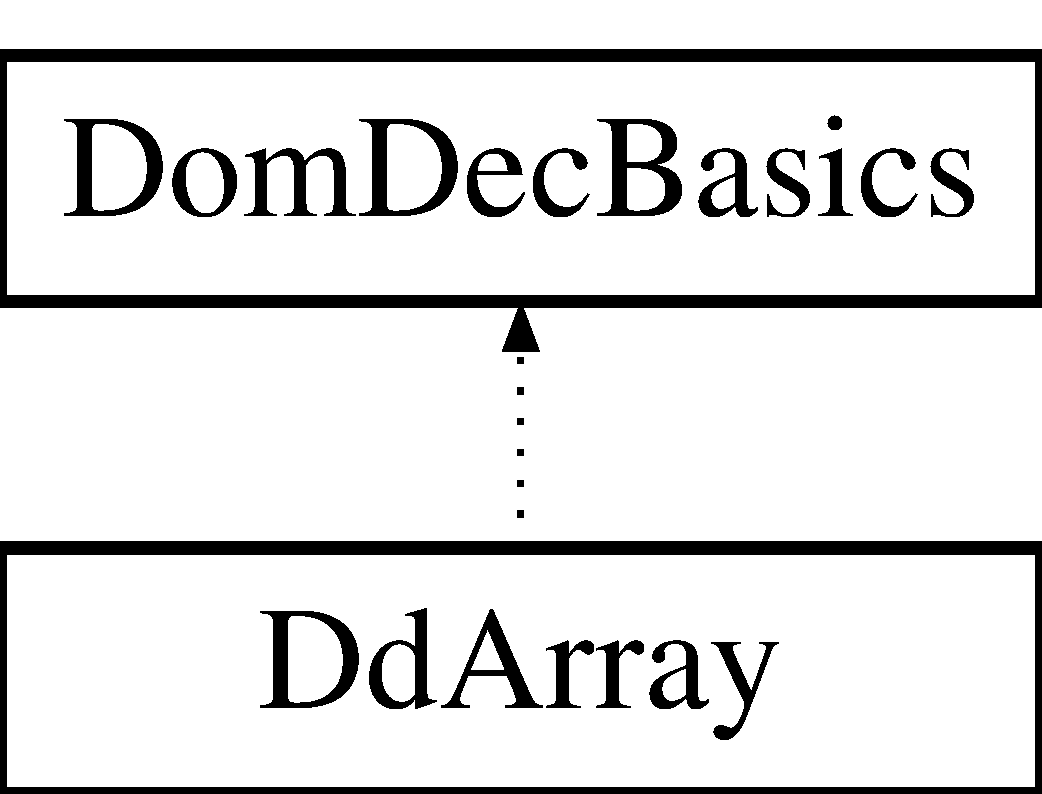
\includegraphics[height=2.000000cm]{classDdArray}
\end{center}
\end{figure}
\subsubsection*{Public Member Functions}
\begin{DoxyCompactItemize}
\item 
\hyperlink{classDdArray_a427b9066964de29a0ecd3d5fe2bedb56}{Dd\+Array} (double Edge\+Ext\mbox{[}3\mbox{]}, int N\+Part, double Cut\+Off)
\begin{DoxyCompactList}\small\item\em Allocate. \end{DoxyCompactList}\item 
void \hyperlink{classDdArray_a98ae2e78109ea826eea71da14c37ce95}{Erase} ()
\begin{DoxyCompactList}\small\item\em Erase the content of the cells. \end{DoxyCompactList}\item 
void \hyperlink{classDdArray_aa71d36872f416feaa853788a7a7a7ef8}{Clear} ()\hypertarget{classDdArray_aa71d36872f416feaa853788a7a7a7ef8}{}\label{classDdArray_aa71d36872f416feaa853788a7a7a7ef8}

\begin{DoxyCompactList}\small\item\em Clear the pairlist. \end{DoxyCompactList}\item 
void \hyperlink{classDdArray_a16bd930c99f12ce47277234de23650ca}{Add\+Part} (int p, double $\ast$Pos)\hypertarget{classDdArray_a16bd930c99f12ce47277234de23650ca}{}\label{classDdArray_a16bd930c99f12ce47277234de23650ca}

\begin{DoxyCompactList}\small\item\em Add a part to the cell. \end{DoxyCompactList}\item 
void \hyperlink{classDdArray_aa81dd095eb9134882b33685338bec68c}{Rem\+Part} (int p, double $\ast$Pos)\hypertarget{classDdArray_aa81dd095eb9134882b33685338bec68c}{}\label{classDdArray_aa81dd095eb9134882b33685338bec68c}

\begin{DoxyCompactList}\small\item\em Remove a part from the cell. \end{DoxyCompactList}\item 
void \hyperlink{classDdArray_a02a69943ed15121906bda20d9c89cb37}{Move\+Part} (int p, double $\ast$Old\+Pos, double $\ast$New\+Pos)\hypertarget{classDdArray_a02a69943ed15121906bda20d9c89cb37}{}\label{classDdArray_a02a69943ed15121906bda20d9c89cb37}

\begin{DoxyCompactList}\small\item\em Move a part. \end{DoxyCompactList}\item 
void \hyperlink{classDdArray_ae468af31d1a530ba0fdaef088c4b9c00}{Swap\+Part} (int p1, double $\ast$Pos1, int p2, double $\ast$Pos2)\hypertarget{classDdArray_ae468af31d1a530ba0fdaef088c4b9c00}{}\label{classDdArray_ae468af31d1a530ba0fdaef088c4b9c00}

\begin{DoxyCompactList}\small\item\em Swap two parts. \end{DoxyCompactList}\item 
void \hyperlink{classDdArray_aadd6f477626e28e8284b9db4649e841d}{Set\+Counters} (int c)\hypertarget{classDdArray_aadd6f477626e28e8284b9db4649e841d}{}\label{classDdArray_aadd6f477626e28e8284b9db4649e841d}

\begin{DoxyCompactList}\small\item\em Set the counters to the initial pointer. \end{DoxyCompactList}\item 
int \hyperlink{classDdArray_af49812231dd30b603631791b87eba9f9}{If\+It\+Cell} (int c)\hypertarget{classDdArray_af49812231dd30b603631791b87eba9f9}{}\label{classDdArray_af49812231dd30b603631791b87eba9f9}

\begin{DoxyCompactList}\small\item\em End the iteration in the cell. \end{DoxyCompactList}\item 
void \hyperlink{classDdArray_af5859063d6fe309152f039205b16014e}{Incr\+Curr} (int c)\hypertarget{classDdArray_af5859063d6fe309152f039205b16014e}{}\label{classDdArray_af5859063d6fe309152f039205b16014e}

\begin{DoxyCompactList}\small\item\em Increase the counters. \end{DoxyCompactList}\item 
int \hyperlink{classDdArray_a1fb1ab9e4e4c98b9860711fdb1fba3b4}{It\+Cell} (int c)\hypertarget{classDdArray_a1fb1ab9e4e4c98b9860711fdb1fba3b4}{}\label{classDdArray_a1fb1ab9e4e4c98b9860711fdb1fba3b4}

\begin{DoxyCompactList}\small\item\em Value of the current particle in the cell c. \end{DoxyCompactList}\item 
int \hyperlink{classDdArray_afe0e4e9746cdae570f8c1efdfd04ac16}{Get\+Nei} (double $\ast$Pos, int $\ast$Nei\+List)\hypertarget{classDdArray_afe0e4e9746cdae570f8c1efdfd04ac16}{}\label{classDdArray_afe0e4e9746cdae570f8c1efdfd04ac16}

\begin{DoxyCompactList}\small\item\em Choose among the different neighbouring lists. \end{DoxyCompactList}\item 
void \hyperlink{classDdArray_aabccb7f79ac6e104734750f00fa72b76}{Couple} (const int c, int $\ast$p1, int $\ast$p2)\hypertarget{classDdArray_aabccb7f79ac6e104734750f00fa72b76}{}\label{classDdArray_aabccb7f79ac6e104734750f00fa72b76}

\begin{DoxyCompactList}\small\item\em Returns the pointed couple of particle. \end{DoxyCompactList}\item 
int \hyperlink{classDdArray_a3896db13faf370f18b2a70c6acd01930}{If\+It\+Couple} (const int c)\hypertarget{classDdArray_a3896db13faf370f18b2a70c6acd01930}{}\label{classDdArray_a3896db13faf370f18b2a70c6acd01930}

\begin{DoxyCompactList}\small\item\em Tell when the loop is over. \end{DoxyCompactList}\item 
void \hyperlink{classDdArray_a0c040f6773c460a8eb46bff752c08d2d}{Incr\+Curr\+List} (const int c)\hypertarget{classDdArray_a0c040f6773c460a8eb46bff752c08d2d}{}\label{classDdArray_a0c040f6773c460a8eb46bff752c08d2d}

\begin{DoxyCompactList}\small\item\em Increment the pointers. \end{DoxyCompactList}\item 
int \hyperlink{classDdArray_a02631cacc3cd393a64b7e78df3734e48}{p\+N\+Cell} ()\hypertarget{classDdArray_a02631cacc3cd393a64b7e78df3734e48}{}\label{classDdArray_a02631cacc3cd393a64b7e78df3734e48}

\begin{DoxyCompactList}\small\item\em Print the number of cells. \end{DoxyCompactList}\item 
void \hyperlink{classDdArray_af5188eb0e6caae79f8bf349bf2345cf2}{Print\+Cell} (const int c)\hypertarget{classDdArray_af5188eb0e6caae79f8bf349bf2345cf2}{}\label{classDdArray_af5188eb0e6caae79f8bf349bf2345cf2}

\begin{DoxyCompactList}\small\item\em Print the content of one cell. \end{DoxyCompactList}\item 
void \hyperlink{classDdArray_a1132024d8fdd721fd6a36781d4235162}{Print\+Cells} ()\hypertarget{classDdArray_a1132024d8fdd721fd6a36781d4235162}{}\label{classDdArray_a1132024d8fdd721fd6a36781d4235162}

\begin{DoxyCompactList}\small\item\em Print the content of every cell. \end{DoxyCompactList}\end{DoxyCompactItemize}
\subsubsection*{Public Attributes}
\begin{DoxyCompactItemize}
\item 
\hyperlink{structDdCell}{Dd\+Cell} $\ast$ \hyperlink{classDdArray_a2bafbd55c3b3a8f13656a8c05660a518}{Cella}\hypertarget{classDdArray_a2bafbd55c3b3a8f13656a8c05660a518}{}\label{classDdArray_a2bafbd55c3b3a8f13656a8c05660a518}

\begin{DoxyCompactList}\small\item\em Cell structure. \end{DoxyCompactList}\end{DoxyCompactItemize}


\subsubsection{Detailed Description}
Domain decomposition using arrays. 

Definition at line 261 of file Cubo.\+h.



\subsubsection{Constructor \& Destructor Documentation}
\index{Dd\+Array@{Dd\+Array}!Dd\+Array@{Dd\+Array}}
\index{Dd\+Array@{Dd\+Array}!Dd\+Array@{Dd\+Array}}
\paragraph[{\texorpdfstring{Dd\+Array(double Edge\+Ext[3], int N\+Part, double Cut\+Off)}{DdArray(double EdgeExt[3], int NPart, double CutOff)}}]{\setlength{\rightskip}{0pt plus 5cm}{\bf Dd\+Array} (
\begin{DoxyParamCaption}
\item[{double}]{Edge\+Ext\mbox{[}3\mbox{]}, }
\item[{int}]{N\+Part, }
\item[{double}]{Cut\+Off}
\end{DoxyParamCaption}
)}\hypertarget{classDdArray_a427b9066964de29a0ecd3d5fe2bedb56}{}\label{classDdArray_a427b9066964de29a0ecd3d5fe2bedb56}


Allocate. 

Every cell contains a stl list of particle. 

Definition at line 634 of file Cubo.\+cpp.



References Dom\+Dec\+Basics\+::\+Cut\+Off, Dom\+Dec\+Basics\+::\+Edge, Dom\+Dec\+Basics\+::\+Inv\+Edge, Dom\+Dec\+Basics\+::\+Mod10, Dom\+Dec\+Basics\+::\+N\+Cell, Dom\+Dec\+Basics\+::\+N\+Part, and Dom\+Dec\+Basics\+::\+N\+Sect.



\subsubsection{Member Function Documentation}
\index{Dd\+Array@{Dd\+Array}!Erase@{Erase}}
\index{Erase@{Erase}!Dd\+Array@{Dd\+Array}}
\paragraph[{\texorpdfstring{Erase()}{Erase()}}]{\setlength{\rightskip}{0pt plus 5cm}void Erase (
\begin{DoxyParamCaption}
{}
\end{DoxyParamCaption}
)}\hypertarget{classDdArray_a98ae2e78109ea826eea71da14c37ce95}{}\label{classDdArray_a98ae2e78109ea826eea71da14c37ce95}


Erase the content of the cells. 

Every cell contains a stl list of particle. 

Definition at line 649 of file Cubo.\+cpp.



References Dom\+Dec\+Basics\+::\+N\+Cell.



The documentation for this class was generated from the following files\+:\begin{DoxyCompactItemize}
\item 
include/Cubo.\+h\item 
src/\+Var\+Data/Cubo.\+cpp\item 
src/\+Var\+Data/Cubo.\+mirror.\+cpp\end{DoxyCompactItemize}

\hypertarget{structDdCell}{\subsection{\-Dd\-Cell \-Struct \-Reference}
\label{structDdCell}\index{\-Dd\-Cell@{\-Dd\-Cell}}
}


\-The array of particles in every cell.  




{\ttfamily \#include $<$\-Cubo.\-h$>$}

\subsubsection*{\-Public \-Attributes}
\begin{DoxyCompactItemize}
\item 
\hypertarget{structDdCell_a42047980ffca3c08f6cce82c43c71373}{list$<$ int $>$ \hyperlink{structDdCell_a42047980ffca3c08f6cce82c43c71373}{\-Part}}\label{structDdCell_a42047980ffca3c08f6cce82c43c71373}

\begin{DoxyCompactList}\small\item\em \-Id of the particle. \end{DoxyCompactList}\end{DoxyCompactItemize}


\subsubsection{\-Detailed \-Description}
\-The array of particles in every cell. 

\-Definition at line 256 of file \-Cubo.\-h.



\-The documentation for this struct was generated from the following file\-:\begin{DoxyCompactItemize}
\item 
include/\-Cubo.\-h\end{DoxyCompactItemize}

\hypertarget{classDdDoubleLoop}{}\subsection{Dd\+Double\+Loop Class Reference}
\label{classDdDoubleLoop}\index{Dd\+Double\+Loop@{Dd\+Double\+Loop}}


Stupid double loop to check the other pair loops.  




{\ttfamily \#include $<$Cubo.\+h$>$}

Inheritance diagram for Dd\+Double\+Loop\+:\begin{figure}[H]
\begin{center}
\leavevmode
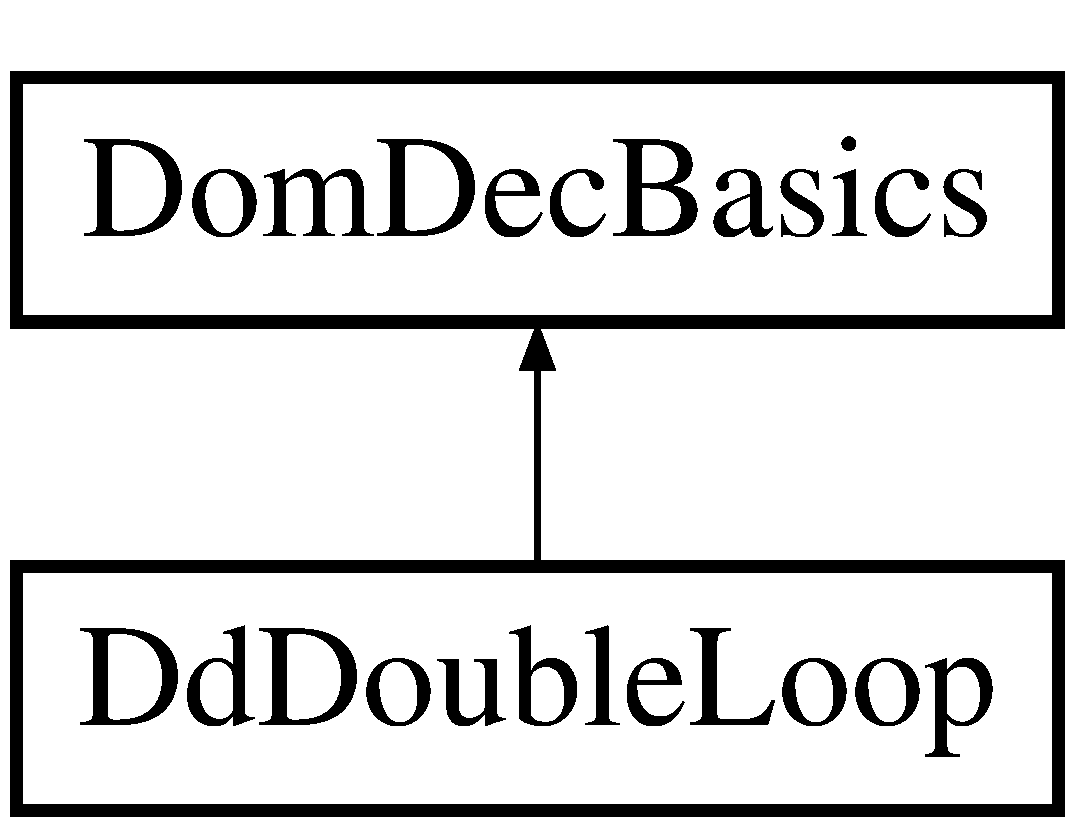
\includegraphics[height=2.000000cm]{classDdDoubleLoop}
\end{center}
\end{figure}
\subsubsection*{Public Member Functions}
\begin{DoxyCompactItemize}
\item 
\hyperlink{classDdDoubleLoop_ac6bab403b0b1578fcb14b996b377d10f}{Dd\+Double\+Loop} (double \hyperlink{classDomDecBasics_a8895c89605e91c6cf7430bad336f77c6}{Edge}\mbox{[}3\mbox{]}, int \hyperlink{classDomDecBasics_abdcc792391d8c5092471dff191de47f4}{N\+Part}, double \hyperlink{classDomDecBasics_af2411aba2dd63fa22b1bc279653ff7a0}{Cut\+Off})
\begin{DoxyCompactList}\small\item\em Allocate. \end{DoxyCompactList}\item 
void \hyperlink{classDdDoubleLoop_a98ae2e78109ea826eea71da14c37ce95}{Erase} ()
\begin{DoxyCompactList}\small\item\em Erase the pairlist. \end{DoxyCompactList}\item 
void \hyperlink{classDdDoubleLoop_aa71d36872f416feaa853788a7a7a7ef8}{Clear} ()\hypertarget{classDdDoubleLoop_aa71d36872f416feaa853788a7a7a7ef8}{}\label{classDdDoubleLoop_aa71d36872f416feaa853788a7a7a7ef8}

\begin{DoxyCompactList}\small\item\em Clear the pairlist. \end{DoxyCompactList}\item 
int \hyperlink{classDdDoubleLoop_a19f169980d772f5f0df4c37de864ef48}{Swap\+Part} (int p1, double $\ast$Pos1, int p2, double $\ast$Pos2)\hypertarget{classDdDoubleLoop_a19f169980d772f5f0df4c37de864ef48}{}\label{classDdDoubleLoop_a19f169980d772f5f0df4c37de864ef48}

\begin{DoxyCompactList}\small\item\em Swap two particles. \end{DoxyCompactList}\item 
void \hyperlink{classDdDoubleLoop_a9a64ea1512bb8d62f9f6a7a80a2bfec9}{Add\+Part} (const int p, double $\ast$Pos)
\begin{DoxyCompactList}\small\item\em Add a particle to the cell c. \end{DoxyCompactList}\item 
void \hyperlink{classDdDoubleLoop_a0f523b65341953255ea5926b23beccf0}{Rem\+Part} (const int p, double $\ast$Pos)
\begin{DoxyCompactList}\small\item\em Remove a particle form the cell c. \end{DoxyCompactList}\item 
void \hyperlink{classDdDoubleLoop_a2c4dbc782956c74becbe3dc2b454d9d0}{Rem\+Part} (const int p)
\begin{DoxyCompactList}\small\item\em Remove the particle p. \end{DoxyCompactList}\item 
void \hyperlink{classDdDoubleLoop_afd35b58ff7908ca3e30a6fa8cee88b4e}{Add\+Part} (const int p, const int c)
\begin{DoxyCompactList}\small\item\em Add a particle to the cell c. \end{DoxyCompactList}\item 
void \hyperlink{classDdDoubleLoop_a5113d105bbcfea8b1b1c50555f21c6fe}{Rem\+Part} (const int p, const int c)
\begin{DoxyCompactList}\small\item\em Remove a particle form the cell c. \end{DoxyCompactList}\item 
void \hyperlink{classDdDoubleLoop_ae2dcbe9a9469a6b50ae328d1cdaae812}{Move\+Part} (const int p, double $\ast$Old\+Pos, double $\ast$New\+Pos)
\begin{DoxyCompactList}\small\item\em Move a particle form the cell c1 to the cell c2. \end{DoxyCompactList}\item 
void \hyperlink{classDdDoubleLoop_a9cc296b765f59b6286128b37d9fedc9f}{Move\+Part} (const int p, double $\ast$New\+Pos)
\begin{DoxyCompactList}\small\item\em Move a particle form the cell c1 to the cell c2. \end{DoxyCompactList}\item 
int \hyperlink{classDdDoubleLoop_ad10ce7d8491ba213cdbc79d4dd4dc013}{Pos\+Ret} (const double Pos\mbox{[}3\mbox{]})\hypertarget{classDdDoubleLoop_ad10ce7d8491ba213cdbc79d4dd4dc013}{}\label{classDdDoubleLoop_ad10ce7d8491ba213cdbc79d4dd4dc013}

\begin{DoxyCompactList}\small\item\em Relative position in the cell. \end{DoxyCompactList}\item 
int \hyperlink{classDdDoubleLoop_a6a2d62432ffa4c509f4a7f1fb5aa7630}{p\+N\+Part} (const int c)\hypertarget{classDdDoubleLoop_a6a2d62432ffa4c509f4a7f1fb5aa7630}{}\label{classDdDoubleLoop_a6a2d62432ffa4c509f4a7f1fb5aa7630}

\begin{DoxyCompactList}\small\item\em \subsubsection*{part in the cell}\end{DoxyCompactList}\item 
int \hyperlink{classDdDoubleLoop_a388622b5e7d2ad20e8ac1a8a951d655f}{p\+N\+Part} ()\hypertarget{classDdDoubleLoop_a388622b5e7d2ad20e8ac1a8a951d655f}{}\label{classDdDoubleLoop_a388622b5e7d2ad20e8ac1a8a951d655f}

\begin{DoxyCompactList}\small\item\em \subsubsection*{part in the class}\end{DoxyCompactList}\item 
int \hyperlink{classDdDoubleLoop_a2d9507d25b2164c0bf4282b38b4a5d88}{p\+Cell} (const int p)\hypertarget{classDdDoubleLoop_a2d9507d25b2164c0bf4282b38b4a5d88}{}\label{classDdDoubleLoop_a2d9507d25b2164c0bf4282b38b4a5d88}

\begin{DoxyCompactList}\small\item\em Print the cell which the particle belong. \end{DoxyCompactList}\item 
int \hyperlink{classDdDoubleLoop_aafe289a3b1eb08ed1b960f1f93e8d836}{First} (const int c)\hypertarget{classDdDoubleLoop_aafe289a3b1eb08ed1b960f1f93e8d836}{}\label{classDdDoubleLoop_aafe289a3b1eb08ed1b960f1f93e8d836}

\begin{DoxyCompactList}\small\item\em First part in the cell. \end{DoxyCompactList}\item 
int \hyperlink{classDdDoubleLoop_a8b3b22221e5f8d516a2c4818bea703ad}{Next} (const int p)\hypertarget{classDdDoubleLoop_a8b3b22221e5f8d516a2c4818bea703ad}{}\label{classDdDoubleLoop_a8b3b22221e5f8d516a2c4818bea703ad}

\begin{DoxyCompactList}\small\item\em Next linked part. \end{DoxyCompactList}\item 
int \hyperlink{classDdDoubleLoop_af415aae03ca33a44460cc0a84bda0f6d}{It\+Cell} (const int c)\hypertarget{classDdDoubleLoop_af415aae03ca33a44460cc0a84bda0f6d}{}\label{classDdDoubleLoop_af415aae03ca33a44460cc0a84bda0f6d}

\begin{DoxyCompactList}\small\item\em Iterate in the cell. \end{DoxyCompactList}\item 
int \hyperlink{classDdDoubleLoop_a7389c3097a5406135ae60ac38ad141f5}{If\+It\+Cell} (const int c)
\begin{DoxyCompactList}\small\item\em Stop the loop and set the counter to zero. \end{DoxyCompactList}\item 
int \hyperlink{classDdDoubleLoop_ab8ed71a5fc65abc128da0367f93803c1}{Set\+Coor\+Numb} (double $\ast$Pos, int p)
\begin{DoxyCompactList}\small\item\em Stop the loop and set the counter to zero. \end{DoxyCompactList}\item 
int \hyperlink{classDdDoubleLoop_afe0e4e9746cdae570f8c1efdfd04ac16}{Get\+Nei} (double $\ast$Pos, int $\ast$Nei\+List)\hypertarget{classDdDoubleLoop_afe0e4e9746cdae570f8c1efdfd04ac16}{}\label{classDdDoubleLoop_afe0e4e9746cdae570f8c1efdfd04ac16}

\begin{DoxyCompactList}\small\item\em Choose among the different neighbouring lists. \end{DoxyCompactList}\item 
void \hyperlink{classDdDoubleLoop_aadd6f477626e28e8284b9db4649e841d}{Set\+Counters} (int c)
\begin{DoxyCompactList}\small\item\em Set the counters to the initial position. \end{DoxyCompactList}\item 
void \hyperlink{classDdDoubleLoop_af5188eb0e6caae79f8bf349bf2345cf2}{Print\+Cell} (const int c)
\begin{DoxyCompactList}\small\item\em Print the particles in a cell. \end{DoxyCompactList}\item 
void \hyperlink{classDdDoubleLoop_a1132024d8fdd721fd6a36781d4235162}{Print\+Cells} ()
\begin{DoxyCompactList}\small\item\em Print the the particles in the cells. \end{DoxyCompactList}\item 
void \hyperlink{classDdDoubleLoop_a74b7b0d716684a7d46993c83795fd9e7}{Set\+Curr} (int p)\hypertarget{classDdDoubleLoop_a74b7b0d716684a7d46993c83795fd9e7}{}\label{classDdDoubleLoop_a74b7b0d716684a7d46993c83795fd9e7}

\begin{DoxyCompactList}\small\item\em Gather information of the neighbouring cells. \end{DoxyCompactList}\item 
void \hyperlink{classDdDoubleLoop_a42eeb7049c078ca89057fbc08726eded}{Next\+Curr} ()\hypertarget{classDdDoubleLoop_a42eeb7049c078ca89057fbc08726eded}{}\label{classDdDoubleLoop_a42eeb7049c078ca89057fbc08726eded}

\begin{DoxyCompactList}\small\item\em Increase the iterator to the next couple. \end{DoxyCompactList}\item 
int \hyperlink{classDdDoubleLoop_a63c5d18d3a487d1a8ab2a5881c6acb38}{If\+Curr} ()\hypertarget{classDdDoubleLoop_a63c5d18d3a487d1a8ab2a5881c6acb38}{}\label{classDdDoubleLoop_a63c5d18d3a487d1a8ab2a5881c6acb38}

\begin{DoxyCompactList}\small\item\em Tell when the curr loop is over. \end{DoxyCompactList}\item 
void \hyperlink{classDdDoubleLoop_ad4860e7b4a26d4b424e5c98b7c6bae09}{Dist2\+Curr} (double $\ast$Dist\+Rel)
\begin{DoxyCompactList}\small\item\em Retrun the squared current interparticle distance. \end{DoxyCompactList}\item 
void \hyperlink{classDdDoubleLoop_abacbda4ce7eed0eee33efe489157ff81}{Print\+List} (const int c)\hypertarget{classDdDoubleLoop_abacbda4ce7eed0eee33efe489157ff81}{}\label{classDdDoubleLoop_abacbda4ce7eed0eee33efe489157ff81}

\begin{DoxyCompactList}\small\item\em Print the the particle list in the cells. \end{DoxyCompactList}\item 
void \hyperlink{classDdDoubleLoop_aff89725be8d743f07f318ef0c06858e1}{Print\+Lists} ()\hypertarget{classDdDoubleLoop_aff89725be8d743f07f318ef0c06858e1}{}\label{classDdDoubleLoop_aff89725be8d743f07f318ef0c06858e1}

\begin{DoxyCompactList}\small\item\em Print the the particle list in the cells. \end{DoxyCompactList}\item 
void \hyperlink{classDdDoubleLoop_a4e589206ab9bc4752d547111d6bba6e7}{Check\+List} ()\hypertarget{classDdDoubleLoop_a4e589206ab9bc4752d547111d6bba6e7}{}\label{classDdDoubleLoop_a4e589206ab9bc4752d547111d6bba6e7}

\begin{DoxyCompactList}\small\item\em Check the list. \end{DoxyCompactList}\item 
void \hyperlink{classDdDoubleLoop_ad6d4b1b657a39ed64c2c45d4706dbcc1}{Check\+Nei} (int p)\hypertarget{classDdDoubleLoop_ad6d4b1b657a39ed64c2c45d4706dbcc1}{}\label{classDdDoubleLoop_ad6d4b1b657a39ed64c2c45d4706dbcc1}

\begin{DoxyCompactList}\small\item\em Check the neighbours. \end{DoxyCompactList}\item 
void \hyperlink{classDdDoubleLoop_ab61672aad0bc83dc07c8efd5a4543fc7}{Incr\+Curr} (const int c)
\begin{DoxyCompactList}\small\item\em Increment the current part in the cell. \end{DoxyCompactList}\item 
void \hyperlink{classDdDoubleLoop_a0c040f6773c460a8eb46bff752c08d2d}{Incr\+Curr\+List} (const int c)\hypertarget{classDdDoubleLoop_a0c040f6773c460a8eb46bff752c08d2d}{}\label{classDdDoubleLoop_a0c040f6773c460a8eb46bff752c08d2d}

\begin{DoxyCompactList}\small\item\em Increment the current iterators in the cell. \end{DoxyCompactList}\end{DoxyCompactItemize}
\subsubsection*{Public Attributes}
\begin{DoxyCompactItemize}
\item 
\hyperlink{classDomCell}{Dom\+Cell} $\ast$ \hyperlink{classDdDoubleLoop_a34021657728255effd1ed64c5d0c5906}{Cella}\hypertarget{classDdDoubleLoop_a34021657728255effd1ed64c5d0c5906}{}\label{classDdDoubleLoop_a34021657728255effd1ed64c5d0c5906}

\begin{DoxyCompactList}\small\item\em Number of particles and iterators per cell. \end{DoxyCompactList}\item 
\hyperlink{structDOMAIN__PART}{D\+O\+M\+A\+I\+N\+\_\+\+P\+A\+RT} $\ast$ \hyperlink{classDdDoubleLoop_a71fca1e109827e1efe1b06f386c44b40}{Pc}\hypertarget{classDdDoubleLoop_a71fca1e109827e1efe1b06f386c44b40}{}\label{classDdDoubleLoop_a71fca1e109827e1efe1b06f386c44b40}

\begin{DoxyCompactList}\small\item\em List of position of the particles. \end{DoxyCompactList}\end{DoxyCompactItemize}


\subsubsection{Detailed Description}
Stupid double loop to check the other pair loops. 

Definition at line 382 of file Cubo.\+h.



\subsubsection{Constructor \& Destructor Documentation}
\index{Dd\+Double\+Loop@{Dd\+Double\+Loop}!Dd\+Double\+Loop@{Dd\+Double\+Loop}}
\index{Dd\+Double\+Loop@{Dd\+Double\+Loop}!Dd\+Double\+Loop@{Dd\+Double\+Loop}}
\paragraph[{\texorpdfstring{Dd\+Double\+Loop(double Edge[3], int N\+Part, double Cut\+Off)}{DdDoubleLoop(double Edge[3], int NPart, double CutOff)}}]{\setlength{\rightskip}{0pt plus 5cm}{\bf Dd\+Double\+Loop} (
\begin{DoxyParamCaption}
\item[{double}]{Edge\mbox{[}3\mbox{]}, }
\item[{int}]{N\+Part, }
\item[{double}]{Cut\+Off}
\end{DoxyParamCaption}
)}\hypertarget{classDdDoubleLoop_ac6bab403b0b1578fcb14b996b377d10f}{}\label{classDdDoubleLoop_ac6bab403b0b1578fcb14b996b377d10f}


Allocate. 

Constructor for the domain decomposition with the linked list. 

Definition at line 855 of file Cubo.\+cpp.



References Dom\+Dec\+Basics\+::\+Edge, Dom\+Dec\+Basics\+::\+Inv\+Edge, Dom\+Dec\+Basics\+::\+Mod10, Dom\+Dec\+Basics\+::\+N\+AllocP, Dom\+Dec\+Basics\+::\+N\+Cell, Dom\+Dec\+Basics\+::\+N\+Part, Dom\+Dec\+Basics\+::\+N\+Sect, Dom\+Dec\+Basics\+::\+Set\+Cut\+Off(), and Dom\+Dec\+Basics\+::\+Sig\+Err().



\subsubsection{Member Function Documentation}
\index{Dd\+Double\+Loop@{Dd\+Double\+Loop}!Erase@{Erase}}
\index{Erase@{Erase}!Dd\+Double\+Loop@{Dd\+Double\+Loop}}
\paragraph[{\texorpdfstring{Erase()}{Erase()}}]{\setlength{\rightskip}{0pt plus 5cm}void Erase (
\begin{DoxyParamCaption}
{}
\end{DoxyParamCaption}
)}\hypertarget{classDdDoubleLoop_a98ae2e78109ea826eea71da14c37ce95}{}\label{classDdDoubleLoop_a98ae2e78109ea826eea71da14c37ce95}


Erase the pairlist. 

Empty the records of the cells. 

Definition at line 878 of file Cubo.\+cpp.



References Dom\+Dec\+Basics\+::\+N\+Cell, and Dom\+Dec\+Basics\+::\+N\+Part.

\index{Dd\+Double\+Loop@{Dd\+Double\+Loop}!Add\+Part@{Add\+Part}}
\index{Add\+Part@{Add\+Part}!Dd\+Double\+Loop@{Dd\+Double\+Loop}}
\paragraph[{\texorpdfstring{Add\+Part(const int p, double $\ast$\+Pos)}{AddPart(const int p, double *Pos)}}]{\setlength{\rightskip}{0pt plus 5cm}void Add\+Part (
\begin{DoxyParamCaption}
\item[{const int}]{p, }
\item[{double $\ast$}]{Pos}
\end{DoxyParamCaption}
)}\hypertarget{classDdDoubleLoop_a9a64ea1512bb8d62f9f6a7a80a2bfec9}{}\label{classDdDoubleLoop_a9a64ea1512bb8d62f9f6a7a80a2bfec9}


Add a particle to the cell c. 

Add a part to the correspondent cell. 

Definition at line 896 of file Cubo.\+cpp.

\index{Dd\+Double\+Loop@{Dd\+Double\+Loop}!Rem\+Part@{Rem\+Part}}
\index{Rem\+Part@{Rem\+Part}!Dd\+Double\+Loop@{Dd\+Double\+Loop}}
\paragraph[{\texorpdfstring{Rem\+Part(const int p, double $\ast$\+Pos)}{RemPart(const int p, double *Pos)}}]{\setlength{\rightskip}{0pt plus 5cm}void Rem\+Part (
\begin{DoxyParamCaption}
\item[{const int}]{p, }
\item[{double $\ast$}]{Pos}
\end{DoxyParamCaption}
)}\hypertarget{classDdDoubleLoop_a0f523b65341953255ea5926b23beccf0}{}\label{classDdDoubleLoop_a0f523b65341953255ea5926b23beccf0}


Remove a particle form the cell c. 

Remove particle from the cell. 

Definition at line 909 of file Cubo.\+cpp.

\index{Dd\+Double\+Loop@{Dd\+Double\+Loop}!Rem\+Part@{Rem\+Part}}
\index{Rem\+Part@{Rem\+Part}!Dd\+Double\+Loop@{Dd\+Double\+Loop}}
\paragraph[{\texorpdfstring{Rem\+Part(const int p)}{RemPart(const int p)}}]{\setlength{\rightskip}{0pt plus 5cm}void Rem\+Part (
\begin{DoxyParamCaption}
\item[{const int}]{p}
\end{DoxyParamCaption}
)}\hypertarget{classDdDoubleLoop_a2c4dbc782956c74becbe3dc2b454d9d0}{}\label{classDdDoubleLoop_a2c4dbc782956c74becbe3dc2b454d9d0}


Remove the particle p. 

Remove a part to the correspondent cell. 

Definition at line 931 of file Cubo.\+cpp.

\index{Dd\+Double\+Loop@{Dd\+Double\+Loop}!Add\+Part@{Add\+Part}}
\index{Add\+Part@{Add\+Part}!Dd\+Double\+Loop@{Dd\+Double\+Loop}}
\paragraph[{\texorpdfstring{Add\+Part(const int p, const int c)}{AddPart(const int p, const int c)}}]{\setlength{\rightskip}{0pt plus 5cm}void Add\+Part (
\begin{DoxyParamCaption}
\item[{const int}]{p, }
\item[{const int}]{c}
\end{DoxyParamCaption}
)}\hypertarget{classDdDoubleLoop_afd35b58ff7908ca3e30a6fa8cee88b4e}{}\label{classDdDoubleLoop_afd35b58ff7908ca3e30a6fa8cee88b4e}


Add a particle to the cell c. 

Add a part to the correspondent cell. 

Definition at line 901 of file Cubo.\+cpp.



References Dom\+Dec\+Basics\+::\+N\+Part.

\index{Dd\+Double\+Loop@{Dd\+Double\+Loop}!Rem\+Part@{Rem\+Part}}
\index{Rem\+Part@{Rem\+Part}!Dd\+Double\+Loop@{Dd\+Double\+Loop}}
\paragraph[{\texorpdfstring{Rem\+Part(const int p, const int c)}{RemPart(const int p, const int c)}}]{\setlength{\rightskip}{0pt plus 5cm}void Rem\+Part (
\begin{DoxyParamCaption}
\item[{const int}]{p, }
\item[{const int}]{c}
\end{DoxyParamCaption}
)}\hypertarget{classDdDoubleLoop_a5113d105bbcfea8b1b1c50555f21c6fe}{}\label{classDdDoubleLoop_a5113d105bbcfea8b1b1c50555f21c6fe}


Remove a particle form the cell c. 

Remove a part to the correspondent cell. 

Definition at line 913 of file Cubo.\+cpp.



References Dom\+Dec\+Basics\+::\+N\+Part.

\index{Dd\+Double\+Loop@{Dd\+Double\+Loop}!Move\+Part@{Move\+Part}}
\index{Move\+Part@{Move\+Part}!Dd\+Double\+Loop@{Dd\+Double\+Loop}}
\paragraph[{\texorpdfstring{Move\+Part(const int p, double $\ast$\+Old\+Pos, double $\ast$\+New\+Pos)}{MovePart(const int p, double *OldPos, double *NewPos)}}]{\setlength{\rightskip}{0pt plus 5cm}void Move\+Part (
\begin{DoxyParamCaption}
\item[{const int}]{p, }
\item[{double $\ast$}]{Old\+Pos, }
\item[{double $\ast$}]{New\+Pos}
\end{DoxyParamCaption}
)}\hypertarget{classDdDoubleLoop_ae2dcbe9a9469a6b50ae328d1cdaae812}{}\label{classDdDoubleLoop_ae2dcbe9a9469a6b50ae328d1cdaae812}


Move a particle form the cell c1 to the cell c2. 

Shift a particle from one position to its new. 

Definition at line 943 of file Cubo.\+cpp.

\index{Dd\+Double\+Loop@{Dd\+Double\+Loop}!Move\+Part@{Move\+Part}}
\index{Move\+Part@{Move\+Part}!Dd\+Double\+Loop@{Dd\+Double\+Loop}}
\paragraph[{\texorpdfstring{Move\+Part(const int p, double $\ast$\+New\+Pos)}{MovePart(const int p, double *NewPos)}}]{\setlength{\rightskip}{0pt plus 5cm}void Move\+Part (
\begin{DoxyParamCaption}
\item[{const int}]{p, }
\item[{double $\ast$}]{New\+Pos}
\end{DoxyParamCaption}
)}\hypertarget{classDdDoubleLoop_a9cc296b765f59b6286128b37d9fedc9f}{}\label{classDdDoubleLoop_a9cc296b765f59b6286128b37d9fedc9f}


Move a particle form the cell c1 to the cell c2. 

Shift a particle from one position to its new. 

Definition at line 939 of file Cubo.\+cpp.

\index{Dd\+Double\+Loop@{Dd\+Double\+Loop}!If\+It\+Cell@{If\+It\+Cell}}
\index{If\+It\+Cell@{If\+It\+Cell}!Dd\+Double\+Loop@{Dd\+Double\+Loop}}
\paragraph[{\texorpdfstring{If\+It\+Cell(const int c)}{IfItCell(const int c)}}]{\setlength{\rightskip}{0pt plus 5cm}int If\+It\+Cell (
\begin{DoxyParamCaption}
\item[{const int}]{c}
\end{DoxyParamCaption}
)}\hypertarget{classDdDoubleLoop_a7389c3097a5406135ae60ac38ad141f5}{}\label{classDdDoubleLoop_a7389c3097a5406135ae60ac38ad141f5}


Stop the loop and set the counter to zero. 

Return 0 when the loop inside the cell is over. 

Definition at line 956 of file Cubo.\+cpp.



References Dom\+Dec\+Basics\+::\+N\+Part, and Dom\+Dec\+Basics\+::p1\+Curr.

\index{Dd\+Double\+Loop@{Dd\+Double\+Loop}!Set\+Coor\+Numb@{Set\+Coor\+Numb}}
\index{Set\+Coor\+Numb@{Set\+Coor\+Numb}!Dd\+Double\+Loop@{Dd\+Double\+Loop}}
\paragraph[{\texorpdfstring{Set\+Coor\+Numb(double $\ast$\+Pos, int p)}{SetCoorNumb(double *Pos, int p)}}]{\setlength{\rightskip}{0pt plus 5cm}int Set\+Coor\+Numb (
\begin{DoxyParamCaption}
\item[{double $\ast$}]{Pos, }
\item[{int}]{p}
\end{DoxyParamCaption}
)}\hypertarget{classDdDoubleLoop_ab8ed71a5fc65abc128da0367f93803c1}{}\label{classDdDoubleLoop_ab8ed71a5fc65abc128da0367f93803c1}


Stop the loop and set the counter to zero. 

Coordination number of the particle in the cell. 

Definition at line 891 of file Cubo.\+cpp.



References Dom\+Dec\+Basics\+::\+Get\+Coor\+Numb().

\index{Dd\+Double\+Loop@{Dd\+Double\+Loop}!Set\+Counters@{Set\+Counters}}
\index{Set\+Counters@{Set\+Counters}!Dd\+Double\+Loop@{Dd\+Double\+Loop}}
\paragraph[{\texorpdfstring{Set\+Counters(int c)}{SetCounters(int c)}}]{\setlength{\rightskip}{0pt plus 5cm}void Set\+Counters (
\begin{DoxyParamCaption}
\item[{int}]{c}
\end{DoxyParamCaption}
)}\hypertarget{classDdDoubleLoop_aadd6f477626e28e8284b9db4649e841d}{}\label{classDdDoubleLoop_aadd6f477626e28e8284b9db4649e841d}


Set the counters to the initial position. 

Set the counters to the first particle of the cell c1 for the first loop. 

Definition at line 947 of file Cubo.\+cpp.



References Dom\+Dec\+Basics\+::c\+Curr, Dom\+Dec\+Basics\+::p1\+Curr, and Dom\+Dec\+Basics\+::p2\+Curr.

\index{Dd\+Double\+Loop@{Dd\+Double\+Loop}!Print\+Cell@{Print\+Cell}}
\index{Print\+Cell@{Print\+Cell}!Dd\+Double\+Loop@{Dd\+Double\+Loop}}
\paragraph[{\texorpdfstring{Print\+Cell(const int c)}{PrintCell(const int c)}}]{\setlength{\rightskip}{0pt plus 5cm}void Print\+Cell (
\begin{DoxyParamCaption}
\item[{const int}]{c}
\end{DoxyParamCaption}
)}\hypertarget{classDdDoubleLoop_af5188eb0e6caae79f8bf349bf2345cf2}{}\label{classDdDoubleLoop_af5188eb0e6caae79f8bf349bf2345cf2}


Print the particles in a cell. 

Print the content of the cell. 

Definition at line 969 of file Cubo.\+cpp.



References Dom\+Dec\+Basics\+::\+N\+Part.

\index{Dd\+Double\+Loop@{Dd\+Double\+Loop}!Print\+Cells@{Print\+Cells}}
\index{Print\+Cells@{Print\+Cells}!Dd\+Double\+Loop@{Dd\+Double\+Loop}}
\paragraph[{\texorpdfstring{Print\+Cells()}{PrintCells()}}]{\setlength{\rightskip}{0pt plus 5cm}void Print\+Cells (
\begin{DoxyParamCaption}
{}
\end{DoxyParamCaption}
)}\hypertarget{classDdDoubleLoop_a1132024d8fdd721fd6a36781d4235162}{}\label{classDdDoubleLoop_a1132024d8fdd721fd6a36781d4235162}


Print the the particles in the cells. 

Print the content of all cells. 

Definition at line 976 of file Cubo.\+cpp.



References Dom\+Dec\+Basics\+::\+N\+Cell, and Dom\+Dec\+Basics\+::\+Print\+Cell().

\index{Dd\+Double\+Loop@{Dd\+Double\+Loop}!Dist2\+Curr@{Dist2\+Curr}}
\index{Dist2\+Curr@{Dist2\+Curr}!Dd\+Double\+Loop@{Dd\+Double\+Loop}}
\paragraph[{\texorpdfstring{Dist2\+Curr(double $\ast$\+Dist\+Rel)}{Dist2Curr(double *DistRel)}}]{\setlength{\rightskip}{0pt plus 5cm}void Dist2\+Curr (
\begin{DoxyParamCaption}
\item[{double $\ast$}]{Dist\+Rel}
\end{DoxyParamCaption}
)}\hypertarget{classDdDoubleLoop_ad4860e7b4a26d4b424e5c98b7c6bae09}{}\label{classDdDoubleLoop_ad4860e7b4a26d4b424e5c98b7c6bae09}


Retrun the squared current interparticle distance. 

Iterate one step and return the position. 

Definition at line 994 of file Cubo.\+cpp.



References Dom\+Dec\+Basics\+::\+Edge, Dom\+Dec\+Basics\+::\+Inv\+Edge, Dom\+Dec\+Basics\+::p1\+Curr, and Dom\+Dec\+Basics\+::p2\+Curr.

\index{Dd\+Double\+Loop@{Dd\+Double\+Loop}!Incr\+Curr@{Incr\+Curr}}
\index{Incr\+Curr@{Incr\+Curr}!Dd\+Double\+Loop@{Dd\+Double\+Loop}}
\paragraph[{\texorpdfstring{Incr\+Curr(const int c)}{IncrCurr(const int c)}}]{\setlength{\rightskip}{0pt plus 5cm}void Incr\+Curr (
\begin{DoxyParamCaption}
\item[{const int}]{c}
\end{DoxyParamCaption}
)}\hypertarget{classDdDoubleLoop_ab61672aad0bc83dc07c8efd5a4543fc7}{}\label{classDdDoubleLoop_ab61672aad0bc83dc07c8efd5a4543fc7}


Increment the current part in the cell. 

Increment the iterator to the next particle. 

Definition at line 961 of file Cubo.\+cpp.



References Dom\+Dec\+Basics\+::\+N\+Part, Dom\+Dec\+Basics\+::p1\+Curr, and Dom\+Dec\+Basics\+::p2\+Curr.



The documentation for this class was generated from the following files\+:\begin{DoxyCompactItemize}
\item 
include/Cubo.\+h\item 
src/\+Var\+Data/Cubo.\+cpp\end{DoxyCompactItemize}

\hypertarget{structDdFixCell}{\subsection{\-Dd\-Fix\-Cell \-Struct \-Reference}
\label{structDdFixCell}\index{\-Dd\-Fix\-Cell@{\-Dd\-Fix\-Cell}}
}


\-The array of particles in every cell.  




{\ttfamily \#include $<$\-Cubo.\-h$>$}

\subsubsection*{\-Public \-Attributes}
\begin{DoxyCompactItemize}
\item 
\hypertarget{structDdFixCell_abdcc792391d8c5092471dff191de47f4}{int \hyperlink{structDdFixCell_abdcc792391d8c5092471dff191de47f4}{\-N\-Part}}\label{structDdFixCell_abdcc792391d8c5092471dff191de47f4}

\begin{DoxyCompactList}\small\item\em \-How many particles. \end{DoxyCompactList}\item 
\hypertarget{structDdFixCell_a9beee0152293e683562b0dccaa209270}{int $\ast$ \hyperlink{structDdFixCell_a9beee0152293e683562b0dccaa209270}{\-Part}}\label{structDdFixCell_a9beee0152293e683562b0dccaa209270}

\begin{DoxyCompactList}\small\item\em \-Id of the particle. \end{DoxyCompactList}\end{DoxyCompactItemize}


\subsubsection{\-Detailed \-Description}
\-The array of particles in every cell. 

\-Definition at line 322 of file \-Cubo.\-h.



\-The documentation for this struct was generated from the following file\-:\begin{DoxyCompactItemize}
\item 
include/\-Cubo.\-h\end{DoxyCompactItemize}

\hypertarget{classDdFixedSize}{}\subsection{Dd\+Fixed\+Size Class Reference}
\label{classDdFixedSize}\index{Dd\+Fixed\+Size@{Dd\+Fixed\+Size}}


Domain decomposition using arrays.  




{\ttfamily \#include $<$Cubo.\+h$>$}

Inheritance diagram for Dd\+Fixed\+Size\+:\begin{figure}[H]
\begin{center}
\leavevmode
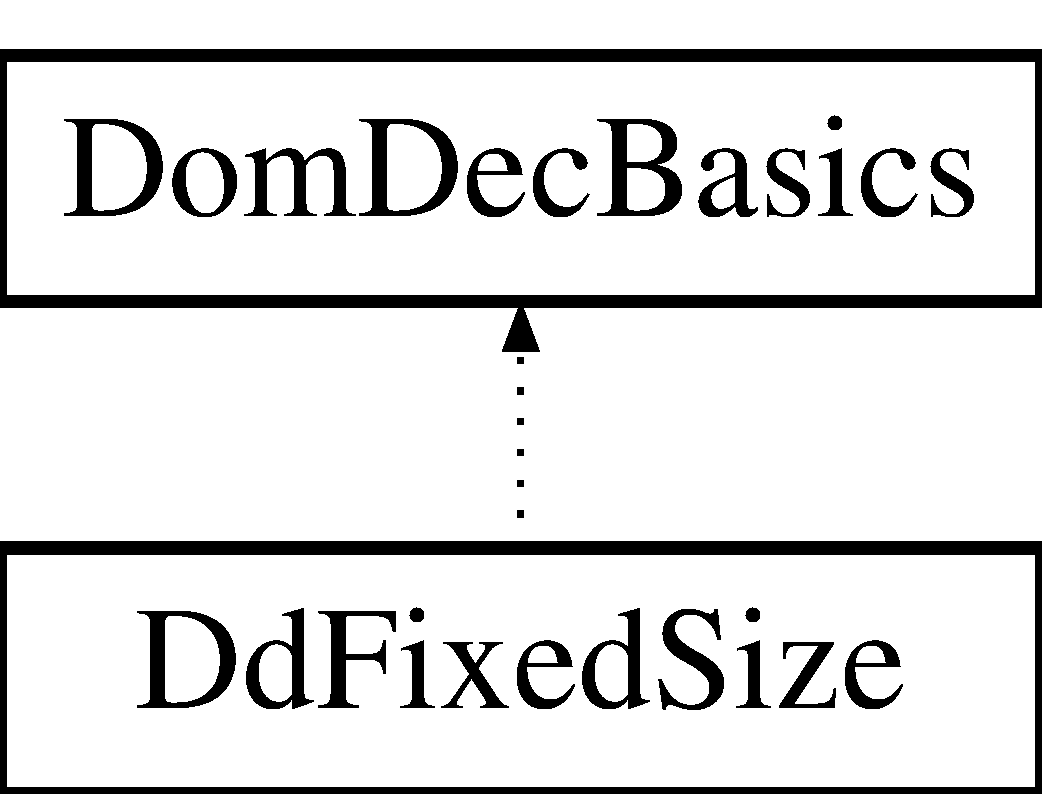
\includegraphics[height=2.000000cm]{classDdFixedSize}
\end{center}
\end{figure}
\subsubsection*{Public Member Functions}
\begin{DoxyCompactItemize}
\item 
\hyperlink{classDdFixedSize_a3b9cc956e6f916c8eb675870cf403b3a}{Dd\+Fixed\+Size} (double Edge\+Ext\mbox{[}3\mbox{]}, int \hyperlink{classDomDecBasics_abdcc792391d8c5092471dff191de47f4}{N\+Part}, double \hyperlink{classDomDecBasics_af2411aba2dd63fa22b1bc279653ff7a0}{Cut\+Off})
\begin{DoxyCompactList}\small\item\em Allocate. \end{DoxyCompactList}\item 
void \hyperlink{classDdFixedSize_a98ae2e78109ea826eea71da14c37ce95}{Erase} ()
\begin{DoxyCompactList}\small\item\em Erase the content of the cells. \end{DoxyCompactList}\item 
void \hyperlink{classDdFixedSize_aa71d36872f416feaa853788a7a7a7ef8}{Clear} ()\hypertarget{classDdFixedSize_aa71d36872f416feaa853788a7a7a7ef8}{}\label{classDdFixedSize_aa71d36872f416feaa853788a7a7a7ef8}

\begin{DoxyCompactList}\small\item\em Clear the pairlist. \end{DoxyCompactList}\item 
void \hyperlink{classDdFixedSize_a16bd930c99f12ce47277234de23650ca}{Add\+Part} (int p, double $\ast$Pos)\hypertarget{classDdFixedSize_a16bd930c99f12ce47277234de23650ca}{}\label{classDdFixedSize_a16bd930c99f12ce47277234de23650ca}

\begin{DoxyCompactList}\small\item\em Add a part to the cell. \end{DoxyCompactList}\item 
void \hyperlink{classDdFixedSize_aa81dd095eb9134882b33685338bec68c}{Rem\+Part} (int p, double $\ast$Pos)\hypertarget{classDdFixedSize_aa81dd095eb9134882b33685338bec68c}{}\label{classDdFixedSize_aa81dd095eb9134882b33685338bec68c}

\begin{DoxyCompactList}\small\item\em Remove a part from the cell. \end{DoxyCompactList}\item 
void \hyperlink{classDdFixedSize_a9e2dba5688a67c185c133e7191e596b3}{Add\+Part} (int p, int c)\hypertarget{classDdFixedSize_a9e2dba5688a67c185c133e7191e596b3}{}\label{classDdFixedSize_a9e2dba5688a67c185c133e7191e596b3}

\begin{DoxyCompactList}\small\item\em Add a part to the cell. \end{DoxyCompactList}\item 
void \hyperlink{classDdFixedSize_ae9da2e58e698bf5bcdca4f880d5579ff}{Rem\+Part} (int p1, int c)\hypertarget{classDdFixedSize_ae9da2e58e698bf5bcdca4f880d5579ff}{}\label{classDdFixedSize_ae9da2e58e698bf5bcdca4f880d5579ff}

\begin{DoxyCompactList}\small\item\em Remove a part from the cell. \end{DoxyCompactList}\item 
void \hyperlink{classDdFixedSize_a02a69943ed15121906bda20d9c89cb37}{Move\+Part} (int p, double $\ast$Old\+Pos, double $\ast$New\+Pos)\hypertarget{classDdFixedSize_a02a69943ed15121906bda20d9c89cb37}{}\label{classDdFixedSize_a02a69943ed15121906bda20d9c89cb37}

\begin{DoxyCompactList}\small\item\em Move a part. \end{DoxyCompactList}\item 
void \hyperlink{classDdFixedSize_ae468af31d1a530ba0fdaef088c4b9c00}{Swap\+Part} (int p1, double $\ast$Pos1, int p2, double $\ast$Pos2)\hypertarget{classDdFixedSize_ae468af31d1a530ba0fdaef088c4b9c00}{}\label{classDdFixedSize_ae468af31d1a530ba0fdaef088c4b9c00}

\begin{DoxyCompactList}\small\item\em Swap two parts. \end{DoxyCompactList}\item 
void \hyperlink{classDdFixedSize_aadd6f477626e28e8284b9db4649e841d}{Set\+Counters} (int c)\hypertarget{classDdFixedSize_aadd6f477626e28e8284b9db4649e841d}{}\label{classDdFixedSize_aadd6f477626e28e8284b9db4649e841d}

\begin{DoxyCompactList}\small\item\em Set the counters to the initial pointer. \end{DoxyCompactList}\item 
int \hyperlink{classDdFixedSize_af49812231dd30b603631791b87eba9f9}{If\+It\+Cell} (int c)\hypertarget{classDdFixedSize_af49812231dd30b603631791b87eba9f9}{}\label{classDdFixedSize_af49812231dd30b603631791b87eba9f9}

\begin{DoxyCompactList}\small\item\em End the iteration in the cell. \end{DoxyCompactList}\item 
void \hyperlink{classDdFixedSize_af5859063d6fe309152f039205b16014e}{Incr\+Curr} (int c)\hypertarget{classDdFixedSize_af5859063d6fe309152f039205b16014e}{}\label{classDdFixedSize_af5859063d6fe309152f039205b16014e}

\begin{DoxyCompactList}\small\item\em Increase the counters. \end{DoxyCompactList}\item 
int \hyperlink{classDdFixedSize_a1fb1ab9e4e4c98b9860711fdb1fba3b4}{It\+Cell} (int c)\hypertarget{classDdFixedSize_a1fb1ab9e4e4c98b9860711fdb1fba3b4}{}\label{classDdFixedSize_a1fb1ab9e4e4c98b9860711fdb1fba3b4}

\begin{DoxyCompactList}\small\item\em Value of the current particle in the cell c. \end{DoxyCompactList}\item 
int \hyperlink{classDdFixedSize_afe0e4e9746cdae570f8c1efdfd04ac16}{Get\+Nei} (double $\ast$Pos, int $\ast$Nei\+List)\hypertarget{classDdFixedSize_afe0e4e9746cdae570f8c1efdfd04ac16}{}\label{classDdFixedSize_afe0e4e9746cdae570f8c1efdfd04ac16}

\begin{DoxyCompactList}\small\item\em Choose among the different neighbouring lists. \end{DoxyCompactList}\item 
void \hyperlink{classDdFixedSize_aabccb7f79ac6e104734750f00fa72b76}{Couple} (const int c, int $\ast$p1, int $\ast$p2)\hypertarget{classDdFixedSize_aabccb7f79ac6e104734750f00fa72b76}{}\label{classDdFixedSize_aabccb7f79ac6e104734750f00fa72b76}

\begin{DoxyCompactList}\small\item\em Returns the pointed couple of particle. \end{DoxyCompactList}\item 
int \hyperlink{classDdFixedSize_a3896db13faf370f18b2a70c6acd01930}{If\+It\+Couple} (const int c)\hypertarget{classDdFixedSize_a3896db13faf370f18b2a70c6acd01930}{}\label{classDdFixedSize_a3896db13faf370f18b2a70c6acd01930}

\begin{DoxyCompactList}\small\item\em Tell when the loop is over. \end{DoxyCompactList}\item 
void \hyperlink{classDdFixedSize_a0c040f6773c460a8eb46bff752c08d2d}{Incr\+Curr\+List} (const int c)\hypertarget{classDdFixedSize_a0c040f6773c460a8eb46bff752c08d2d}{}\label{classDdFixedSize_a0c040f6773c460a8eb46bff752c08d2d}

\begin{DoxyCompactList}\small\item\em Increment the pointers. \end{DoxyCompactList}\item 
void \hyperlink{classDdFixedSize_af5188eb0e6caae79f8bf349bf2345cf2}{Print\+Cell} (const int c)\hypertarget{classDdFixedSize_af5188eb0e6caae79f8bf349bf2345cf2}{}\label{classDdFixedSize_af5188eb0e6caae79f8bf349bf2345cf2}

\begin{DoxyCompactList}\small\item\em Print the content of one cell. \end{DoxyCompactList}\item 
void \hyperlink{classDdFixedSize_a1132024d8fdd721fd6a36781d4235162}{Print\+Cells} ()\hypertarget{classDdFixedSize_a1132024d8fdd721fd6a36781d4235162}{}\label{classDdFixedSize_a1132024d8fdd721fd6a36781d4235162}

\begin{DoxyCompactList}\small\item\em Print the content of every cell. \end{DoxyCompactList}\end{DoxyCompactItemize}
\subsubsection*{Public Attributes}
\begin{DoxyCompactItemize}
\item 
\hyperlink{structDdFixCell}{Dd\+Fix\+Cell} $\ast$ \hyperlink{classDdFixedSize_a02d24fa5352eb35985cb524dcee6c5a3}{Cella}\hypertarget{classDdFixedSize_a02d24fa5352eb35985cb524dcee6c5a3}{}\label{classDdFixedSize_a02d24fa5352eb35985cb524dcee6c5a3}

\begin{DoxyCompactList}\small\item\em Cell structure. \end{DoxyCompactList}\end{DoxyCompactItemize}


\subsubsection{Detailed Description}
Domain decomposition using arrays. 

Definition at line 329 of file Cubo.\+h.



\subsubsection{Constructor \& Destructor Documentation}
\index{Dd\+Fixed\+Size@{Dd\+Fixed\+Size}!Dd\+Fixed\+Size@{Dd\+Fixed\+Size}}
\index{Dd\+Fixed\+Size@{Dd\+Fixed\+Size}!Dd\+Fixed\+Size@{Dd\+Fixed\+Size}}
\paragraph[{\texorpdfstring{Dd\+Fixed\+Size(double Edge\+Ext[3], int N\+Part, double Cut\+Off)}{DdFixedSize(double EdgeExt[3], int NPart, double CutOff)}}]{\setlength{\rightskip}{0pt plus 5cm}{\bf Dd\+Fixed\+Size} (
\begin{DoxyParamCaption}
\item[{double}]{Edge\+Ext\mbox{[}3\mbox{]}, }
\item[{int}]{N\+Part, }
\item[{double}]{Cut\+Off}
\end{DoxyParamCaption}
)}\hypertarget{classDdFixedSize_a3b9cc956e6f916c8eb675870cf403b3a}{}\label{classDdFixedSize_a3b9cc956e6f916c8eb675870cf403b3a}


Allocate. 

Every cell contains a stl list of particle. 

Definition at line 728 of file Cubo.\+cpp.



References Dom\+Dec\+Basics\+::\+Cut\+Off, Dom\+Dec\+Basics\+::\+Edge, Dom\+Dec\+Basics\+::\+Inv\+Edge, Dom\+Dec\+Basics\+::\+Mod10, Dom\+Dec\+Basics\+::\+N\+Cell, Dom\+Dec\+Basics\+::\+N\+Part, Dom\+Dec\+Basics\+::\+N\+Sect, and Dd\+Fix\+Cell\+::\+Part.



\subsubsection{Member Function Documentation}
\index{Dd\+Fixed\+Size@{Dd\+Fixed\+Size}!Erase@{Erase}}
\index{Erase@{Erase}!Dd\+Fixed\+Size@{Dd\+Fixed\+Size}}
\paragraph[{\texorpdfstring{Erase()}{Erase()}}]{\setlength{\rightskip}{0pt plus 5cm}void Erase (
\begin{DoxyParamCaption}
{}
\end{DoxyParamCaption}
)}\hypertarget{classDdFixedSize_a98ae2e78109ea826eea71da14c37ce95}{}\label{classDdFixedSize_a98ae2e78109ea826eea71da14c37ce95}


Erase the content of the cells. 

Every cell contains a stl list of particle. 

Definition at line 747 of file Cubo.\+cpp.



References Dom\+Dec\+Basics\+::\+N\+Cell.



The documentation for this class was generated from the following files\+:\begin{DoxyCompactItemize}
\item 
include/Cubo.\+h\item 
src/\+Var\+Data/Cubo.\+cpp\item 
src/\+Var\+Data/Cubo.\+mirror.\+cpp\end{DoxyCompactItemize}

\hypertarget{classDdLinkedList}{}\subsection{Dd\+Linked\+List Class Reference}
\label{classDdLinkedList}\index{Dd\+Linked\+List@{Dd\+Linked\+List}}


Domain decomposition as pointer to linked particles.  




{\ttfamily \#include $<$Cubo.\+h$>$}

Inheritance diagram for Dd\+Linked\+List\+:\begin{figure}[H]
\begin{center}
\leavevmode
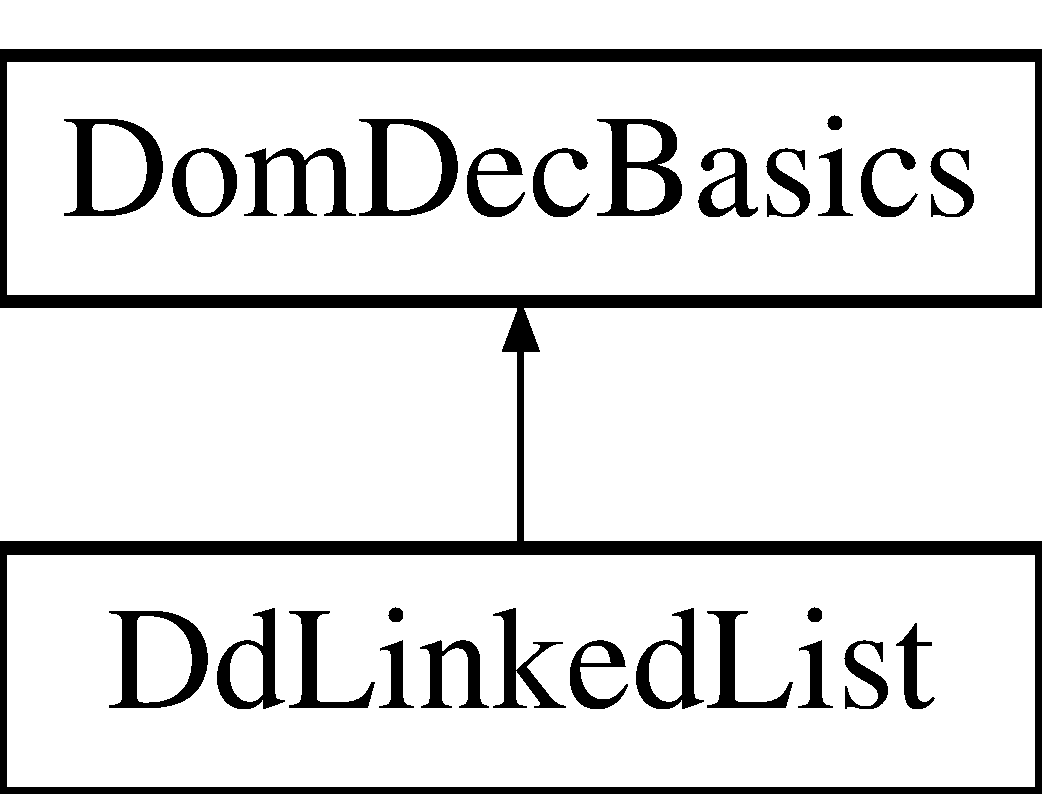
\includegraphics[height=2.000000cm]{classDdLinkedList}
\end{center}
\end{figure}
\subsubsection*{Public Member Functions}
\begin{DoxyCompactItemize}
\item 
\hyperlink{classDdLinkedList_aaf16124b5aa0b2a6597b9363f1a1c247}{Dd\+Linked\+List} (double \hyperlink{classDomDecBasics_a8895c89605e91c6cf7430bad336f77c6}{Edge}\mbox{[}3\mbox{]}, int \hyperlink{classDomDecBasics_abdcc792391d8c5092471dff191de47f4}{N\+Part}, double \hyperlink{classDomDecBasics_af2411aba2dd63fa22b1bc279653ff7a0}{Cut\+Off})
\begin{DoxyCompactList}\small\item\em Allocate. \end{DoxyCompactList}\item 
void \hyperlink{classDdLinkedList_a98ae2e78109ea826eea71da14c37ce95}{Erase} ()
\begin{DoxyCompactList}\small\item\em Erase the pairlist. \end{DoxyCompactList}\item 
void \hyperlink{classDdLinkedList_aa71d36872f416feaa853788a7a7a7ef8}{Clear} ()\hypertarget{classDdLinkedList_aa71d36872f416feaa853788a7a7a7ef8}{}\label{classDdLinkedList_aa71d36872f416feaa853788a7a7a7ef8}

\begin{DoxyCompactList}\small\item\em Clear the pairlist. \end{DoxyCompactList}\item 
int \hyperlink{classDdLinkedList_ae468af31d1a530ba0fdaef088c4b9c00}{Swap\+Part} (int p1, double $\ast$Pos1, int p2, double $\ast$Pos2)\hypertarget{classDdLinkedList_ae468af31d1a530ba0fdaef088c4b9c00}{}\label{classDdLinkedList_ae468af31d1a530ba0fdaef088c4b9c00}

\begin{DoxyCompactList}\small\item\em Swap two particles. \end{DoxyCompactList}\item 
void \hyperlink{classDdLinkedList_a9a64ea1512bb8d62f9f6a7a80a2bfec9}{Add\+Part} (const int p, double $\ast$Pos)
\begin{DoxyCompactList}\small\item\em Add a particle to the cell c. \end{DoxyCompactList}\item 
void \hyperlink{classDdLinkedList_a0f523b65341953255ea5926b23beccf0}{Rem\+Part} (const int p, double $\ast$Pos)
\begin{DoxyCompactList}\small\item\em Remove a particle form the cell c. \end{DoxyCompactList}\item 
void \hyperlink{classDdLinkedList_a2c4dbc782956c74becbe3dc2b454d9d0}{Rem\+Part} (const int p)
\begin{DoxyCompactList}\small\item\em Remove the particle p. \end{DoxyCompactList}\item 
void \hyperlink{classDdLinkedList_afd35b58ff7908ca3e30a6fa8cee88b4e}{Add\+Part} (const int p, const int c)
\begin{DoxyCompactList}\small\item\em Add a particle to the cell c. \end{DoxyCompactList}\item 
void \hyperlink{classDdLinkedList_a5113d105bbcfea8b1b1c50555f21c6fe}{Rem\+Part} (const int p, const int c)
\begin{DoxyCompactList}\small\item\em Remove a particle form the cell c. \end{DoxyCompactList}\item 
void \hyperlink{classDdLinkedList_ae2dcbe9a9469a6b50ae328d1cdaae812}{Move\+Part} (const int p, double $\ast$Old\+Pos, double $\ast$New\+Pos)
\begin{DoxyCompactList}\small\item\em Move a particle form the cell c1 to the cell c2. \end{DoxyCompactList}\item 
void \hyperlink{classDdLinkedList_a9cc296b765f59b6286128b37d9fedc9f}{Move\+Part} (const int p, double $\ast$New\+Pos)
\begin{DoxyCompactList}\small\item\em Move a particle form the cell c1 to the cell c2. \end{DoxyCompactList}\item 
int \hyperlink{classDdLinkedList_ad10ce7d8491ba213cdbc79d4dd4dc013}{Pos\+Ret} (const double Pos\mbox{[}3\mbox{]})\hypertarget{classDdLinkedList_ad10ce7d8491ba213cdbc79d4dd4dc013}{}\label{classDdLinkedList_ad10ce7d8491ba213cdbc79d4dd4dc013}

\begin{DoxyCompactList}\small\item\em Relative position in the cell. \end{DoxyCompactList}\item 
int \hyperlink{classDdLinkedList_a6a2d62432ffa4c509f4a7f1fb5aa7630}{p\+N\+Part} (const int c)\hypertarget{classDdLinkedList_a6a2d62432ffa4c509f4a7f1fb5aa7630}{}\label{classDdLinkedList_a6a2d62432ffa4c509f4a7f1fb5aa7630}

\begin{DoxyCompactList}\small\item\em \subsubsection*{part in the cell}\end{DoxyCompactList}\item 
int \hyperlink{classDdLinkedList_a388622b5e7d2ad20e8ac1a8a951d655f}{p\+N\+Part} ()\hypertarget{classDdLinkedList_a388622b5e7d2ad20e8ac1a8a951d655f}{}\label{classDdLinkedList_a388622b5e7d2ad20e8ac1a8a951d655f}

\begin{DoxyCompactList}\small\item\em \subsubsection*{part in the class}\end{DoxyCompactList}\item 
int \hyperlink{classDdLinkedList_a2d9507d25b2164c0bf4282b38b4a5d88}{p\+Cell} (const int p)\hypertarget{classDdLinkedList_a2d9507d25b2164c0bf4282b38b4a5d88}{}\label{classDdLinkedList_a2d9507d25b2164c0bf4282b38b4a5d88}

\begin{DoxyCompactList}\small\item\em Print the cell which the particle belong. \end{DoxyCompactList}\item 
int \hyperlink{classDdLinkedList_aafe289a3b1eb08ed1b960f1f93e8d836}{First} (const int c)\hypertarget{classDdLinkedList_aafe289a3b1eb08ed1b960f1f93e8d836}{}\label{classDdLinkedList_aafe289a3b1eb08ed1b960f1f93e8d836}

\begin{DoxyCompactList}\small\item\em First part in the cell. \end{DoxyCompactList}\item 
int \hyperlink{classDdLinkedList_a8b3b22221e5f8d516a2c4818bea703ad}{Next} (const int p)\hypertarget{classDdLinkedList_a8b3b22221e5f8d516a2c4818bea703ad}{}\label{classDdLinkedList_a8b3b22221e5f8d516a2c4818bea703ad}

\begin{DoxyCompactList}\small\item\em Next linked part. \end{DoxyCompactList}\item 
int \hyperlink{classDdLinkedList_af415aae03ca33a44460cc0a84bda0f6d}{It\+Cell} (const int c)\hypertarget{classDdLinkedList_af415aae03ca33a44460cc0a84bda0f6d}{}\label{classDdLinkedList_af415aae03ca33a44460cc0a84bda0f6d}

\begin{DoxyCompactList}\small\item\em Iterate in the cell. \end{DoxyCompactList}\item 
int \hyperlink{classDdLinkedList_a7389c3097a5406135ae60ac38ad141f5}{If\+It\+Cell} (const int c)
\begin{DoxyCompactList}\small\item\em Stop the loop and set the counter to zero. \end{DoxyCompactList}\item 
int \hyperlink{classDdLinkedList_a3896db13faf370f18b2a70c6acd01930}{If\+It\+Couple} (const int c)
\begin{DoxyCompactList}\small\item\em Stop the loop and set the counter to zero. \end{DoxyCompactList}\item 
int \hyperlink{classDdLinkedList_ab8ed71a5fc65abc128da0367f93803c1}{Set\+Coor\+Numb} (double $\ast$Pos, int p)
\begin{DoxyCompactList}\small\item\em Set the coordination umber to the part p. \end{DoxyCompactList}\item 
int \hyperlink{classDdLinkedList_afe0e4e9746cdae570f8c1efdfd04ac16}{Get\+Nei} (double $\ast$Pos, int $\ast$Nei\+List)\hypertarget{classDdLinkedList_afe0e4e9746cdae570f8c1efdfd04ac16}{}\label{classDdLinkedList_afe0e4e9746cdae570f8c1efdfd04ac16}

\begin{DoxyCompactList}\small\item\em Choose among the different neighbouring lists. \end{DoxyCompactList}\item 
void \hyperlink{classDdLinkedList_aadd6f477626e28e8284b9db4649e841d}{Set\+Counters} (int c)
\begin{DoxyCompactList}\small\item\em Set the counters to the initial position. \end{DoxyCompactList}\item 
void \hyperlink{classDdLinkedList_aabccb7f79ac6e104734750f00fa72b76}{Couple} (const int c, int $\ast$p1, int $\ast$p2)
\begin{DoxyCompactList}\small\item\em Iterates along all couples. \end{DoxyCompactList}\item 
void \hyperlink{classDdLinkedList_af5188eb0e6caae79f8bf349bf2345cf2}{Print\+Cell} (const int c)
\begin{DoxyCompactList}\small\item\em Print the particles in a cell. \end{DoxyCompactList}\item 
void \hyperlink{classDdLinkedList_a1132024d8fdd721fd6a36781d4235162}{Print\+Cells} ()
\begin{DoxyCompactList}\small\item\em Print the the particles in the cells. \end{DoxyCompactList}\item 
void \hyperlink{classDdLinkedList_a74b7b0d716684a7d46993c83795fd9e7}{Set\+Curr} (int p)
\begin{DoxyCompactList}\small\item\em Gather information of the neighbouring cells. \end{DoxyCompactList}\item 
void \hyperlink{classDdLinkedList_acbfe19bc52a783e62b9ed1a4548020be}{Set\+Curr\+Ghost} (double $\ast$Pos)\hypertarget{classDdLinkedList_acbfe19bc52a783e62b9ed1a4548020be}{}\label{classDdLinkedList_acbfe19bc52a783e62b9ed1a4548020be}

\begin{DoxyCompactList}\small\item\em Gather information of the neighbouring cells. \end{DoxyCompactList}\item 
void \hyperlink{classDdLinkedList_a42eeb7049c078ca89057fbc08726eded}{Next\+Curr} ()\hypertarget{classDdLinkedList_a42eeb7049c078ca89057fbc08726eded}{}\label{classDdLinkedList_a42eeb7049c078ca89057fbc08726eded}

\begin{DoxyCompactList}\small\item\em Increase the iterator to the next couple. \end{DoxyCompactList}\item 
void \hyperlink{classDdLinkedList_a570f38547139c0b1405fde555f276b9c}{Next\+Curr\+Ghost} ()\hypertarget{classDdLinkedList_a570f38547139c0b1405fde555f276b9c}{}\label{classDdLinkedList_a570f38547139c0b1405fde555f276b9c}

\begin{DoxyCompactList}\small\item\em Increase the iterator to the next couple. \end{DoxyCompactList}\item 
int \hyperlink{classDdLinkedList_a63c5d18d3a487d1a8ab2a5881c6acb38}{If\+Curr} ()
\begin{DoxyCompactList}\small\item\em Tell when the curr loop is over. \end{DoxyCompactList}\item 
int \hyperlink{classDdLinkedList_a1473510db4cdf7f15b2875ad737e351e}{If\+Curr\+Ghost} ()\hypertarget{classDdLinkedList_a1473510db4cdf7f15b2875ad737e351e}{}\label{classDdLinkedList_a1473510db4cdf7f15b2875ad737e351e}

\begin{DoxyCompactList}\small\item\em Tell when the curr loop is over. \end{DoxyCompactList}\item 
void \hyperlink{classDdLinkedList_ad4860e7b4a26d4b424e5c98b7c6bae09}{Dist2\+Curr} (double $\ast$Dist\+Rel)
\begin{DoxyCompactList}\small\item\em Retrun the squared current interparticle distance. \end{DoxyCompactList}\item 
void \hyperlink{classDdLinkedList_a88042fab4b1c26be298e1b40f7409cd3}{Dist2\+Curr\+Ghost} (double $\ast$Dist\+Rel)
\begin{DoxyCompactList}\small\item\em Retrun the squared current interparticle distance. \end{DoxyCompactList}\item 
void \hyperlink{classDdLinkedList_abacbda4ce7eed0eee33efe489157ff81}{Print\+List} (const int c)\hypertarget{classDdLinkedList_abacbda4ce7eed0eee33efe489157ff81}{}\label{classDdLinkedList_abacbda4ce7eed0eee33efe489157ff81}

\begin{DoxyCompactList}\small\item\em Print the the particle list in the cells. \end{DoxyCompactList}\item 
void \hyperlink{classDdLinkedList_aff89725be8d743f07f318ef0c06858e1}{Print\+Lists} ()\hypertarget{classDdLinkedList_aff89725be8d743f07f318ef0c06858e1}{}\label{classDdLinkedList_aff89725be8d743f07f318ef0c06858e1}

\begin{DoxyCompactList}\small\item\em Print the the particle list in the cells. \end{DoxyCompactList}\item 
void \hyperlink{classDdLinkedList_a4e589206ab9bc4752d547111d6bba6e7}{Check\+List} ()\hypertarget{classDdLinkedList_a4e589206ab9bc4752d547111d6bba6e7}{}\label{classDdLinkedList_a4e589206ab9bc4752d547111d6bba6e7}

\begin{DoxyCompactList}\small\item\em Check the list. \end{DoxyCompactList}\item 
void \hyperlink{classDdLinkedList_ad6d4b1b657a39ed64c2c45d4706dbcc1}{Check\+Nei} (int p)\hypertarget{classDdLinkedList_ad6d4b1b657a39ed64c2c45d4706dbcc1}{}\label{classDdLinkedList_ad6d4b1b657a39ed64c2c45d4706dbcc1}

\begin{DoxyCompactList}\small\item\em Check the neighbours. \end{DoxyCompactList}\item 
void \hyperlink{classDdLinkedList_ab61672aad0bc83dc07c8efd5a4543fc7}{Incr\+Curr} (const int c)
\begin{DoxyCompactList}\small\item\em Increment the current part in the cell. \end{DoxyCompactList}\item 
void \hyperlink{classDdLinkedList_a0c040f6773c460a8eb46bff752c08d2d}{Incr\+Curr\+List} (const int c)
\begin{DoxyCompactList}\small\item\em Increment the current iterators in the cell. \end{DoxyCompactList}\item 
int \hyperlink{classDdLinkedList_a0d08a6310d088c729b6b1e496203a3d9}{Find\+Closest} (int p1)\hypertarget{classDdLinkedList_a0d08a6310d088c729b6b1e496203a3d9}{}\label{classDdLinkedList_a0d08a6310d088c729b6b1e496203a3d9}

\begin{DoxyCompactList}\small\item\em Find the closest neighbour. \end{DoxyCompactList}\end{DoxyCompactItemize}
\subsubsection*{Public Attributes}
\begin{DoxyCompactItemize}
\item 
\hyperlink{classDomCell}{Dom\+Cell} $\ast$ \hyperlink{classDdLinkedList_a34021657728255effd1ed64c5d0c5906}{Cella}\hypertarget{classDdLinkedList_a34021657728255effd1ed64c5d0c5906}{}\label{classDdLinkedList_a34021657728255effd1ed64c5d0c5906}

\begin{DoxyCompactList}\small\item\em Number of particles and iterators per cell. \end{DoxyCompactList}\item 
\hyperlink{structDOMAIN__PART}{D\+O\+M\+A\+I\+N\+\_\+\+P\+A\+RT} $\ast$ \hyperlink{classDdLinkedList_a71fca1e109827e1efe1b06f386c44b40}{Pc}\hypertarget{classDdLinkedList_a71fca1e109827e1efe1b06f386c44b40}{}\label{classDdLinkedList_a71fca1e109827e1efe1b06f386c44b40}

\begin{DoxyCompactList}\small\item\em List of position of the particles. \end{DoxyCompactList}\end{DoxyCompactItemize}


\subsubsection{Detailed Description}
Domain decomposition as pointer to linked particles. 

Definition at line 162 of file Cubo.\+h.



\subsubsection{Constructor \& Destructor Documentation}
\index{Dd\+Linked\+List@{Dd\+Linked\+List}!Dd\+Linked\+List@{Dd\+Linked\+List}}
\index{Dd\+Linked\+List@{Dd\+Linked\+List}!Dd\+Linked\+List@{Dd\+Linked\+List}}
\paragraph[{\texorpdfstring{Dd\+Linked\+List(double Edge[3], int N\+Part, double Cut\+Off)}{DdLinkedList(double Edge[3], int NPart, double CutOff)}}]{\setlength{\rightskip}{0pt plus 5cm}{\bf Dd\+Linked\+List} (
\begin{DoxyParamCaption}
\item[{double}]{Edge\mbox{[}3\mbox{]}, }
\item[{int}]{N\+Part, }
\item[{double}]{Cut\+Off}
\end{DoxyParamCaption}
)}\hypertarget{classDdLinkedList_aaf16124b5aa0b2a6597b9363f1a1c247}{}\label{classDdLinkedList_aaf16124b5aa0b2a6597b9363f1a1c247}


Allocate. 

Constructor for the domain decomposition with the linked list. 

Definition at line 232 of file Cubo.\+cpp.



References Dom\+Dec\+Basics\+::\+Edge, Dom\+Dec\+Basics\+::\+Inv\+Edge, Dom\+Dec\+Basics\+::\+Mod10, Dom\+Dec\+Basics\+::\+N\+AllocP, Dom\+Dec\+Basics\+::\+N\+Cell, Dom\+Dec\+Basics\+::\+N\+Part, Dom\+Dec\+Basics\+::\+N\+Sect, Dom\+Dec\+Basics\+::\+Set\+Cut\+Off(), and Dom\+Dec\+Basics\+::\+Sig\+Err().



\subsubsection{Member Function Documentation}
\index{Dd\+Linked\+List@{Dd\+Linked\+List}!Erase@{Erase}}
\index{Erase@{Erase}!Dd\+Linked\+List@{Dd\+Linked\+List}}
\paragraph[{\texorpdfstring{Erase()}{Erase()}}]{\setlength{\rightskip}{0pt plus 5cm}void Erase (
\begin{DoxyParamCaption}
{}
\end{DoxyParamCaption}
)}\hypertarget{classDdLinkedList_a98ae2e78109ea826eea71da14c37ce95}{}\label{classDdLinkedList_a98ae2e78109ea826eea71da14c37ce95}


Erase the pairlist. 

Empty the records of the cells. 

Definition at line 258 of file Cubo.\+cpp.



References Dom\+Dec\+Basics\+::\+N\+Cell, and Dom\+Dec\+Basics\+::\+N\+Part.



Referenced by Forces\+::\+Dynamics(), Forces\+::\+Minimal\+Nrg(), and Forces\+::\+Re\+Open().

\index{Dd\+Linked\+List@{Dd\+Linked\+List}!Add\+Part@{Add\+Part}}
\index{Add\+Part@{Add\+Part}!Dd\+Linked\+List@{Dd\+Linked\+List}}
\paragraph[{\texorpdfstring{Add\+Part(const int p, double $\ast$\+Pos)}{AddPart(const int p, double *Pos)}}]{\setlength{\rightskip}{0pt plus 5cm}void Add\+Part (
\begin{DoxyParamCaption}
\item[{const int}]{p, }
\item[{double $\ast$}]{Pos}
\end{DoxyParamCaption}
)}\hypertarget{classDdLinkedList_a9a64ea1512bb8d62f9f6a7a80a2bfec9}{}\label{classDdLinkedList_a9a64ea1512bb8d62f9f6a7a80a2bfec9}


Add a particle to the cell c. 

Add a part to the correspondent cell. 

Definition at line 276 of file Cubo.\+cpp.



References Dom\+Dec\+Basics\+::p\+Cella().



Referenced by Forces\+::\+Alloc\+Method(), Var\+Data\+::\+Connect\+Line\+Chain(), Var\+Data\+::\+Connect\+Line\+Chain3(), Forces\+::\+Consider\+Ch(), Forces\+::\+Dynamics(), Var\+Data\+::\+Find\+Neighbours(), Forces\+::\+Insert\+Bead(), Forces\+::\+Insert\+Ch\+Bias(), Forces\+::\+Minimal\+Nrg(), Forces\+::\+Remove\+Ch\+Bias(), and Forces\+::\+Re\+Open().

\index{Dd\+Linked\+List@{Dd\+Linked\+List}!Rem\+Part@{Rem\+Part}}
\index{Rem\+Part@{Rem\+Part}!Dd\+Linked\+List@{Dd\+Linked\+List}}
\paragraph[{\texorpdfstring{Rem\+Part(const int p, double $\ast$\+Pos)}{RemPart(const int p, double *Pos)}}]{\setlength{\rightskip}{0pt plus 5cm}void Rem\+Part (
\begin{DoxyParamCaption}
\item[{const int}]{p, }
\item[{double $\ast$}]{Pos}
\end{DoxyParamCaption}
)}\hypertarget{classDdLinkedList_a0f523b65341953255ea5926b23beccf0}{}\label{classDdLinkedList_a0f523b65341953255ea5926b23beccf0}


Remove a particle form the cell c. 

Remove particle from the cell. 

Definition at line 307 of file Cubo.\+cpp.



References Dom\+Dec\+Basics\+::p\+Cella().



Referenced by Forces\+::\+Ignore\+Ch(), Forces\+::\+Rem\+Ch\+From\+Sys(), Forces\+::\+Remove\+Ch\+Bias(), Forces\+::\+Try\+Insert(), Forces\+::\+Try\+Remove(), and Forces\+::\+Widom\+Insert().

\index{Dd\+Linked\+List@{Dd\+Linked\+List}!Rem\+Part@{Rem\+Part}}
\index{Rem\+Part@{Rem\+Part}!Dd\+Linked\+List@{Dd\+Linked\+List}}
\paragraph[{\texorpdfstring{Rem\+Part(const int p)}{RemPart(const int p)}}]{\setlength{\rightskip}{0pt plus 5cm}void Rem\+Part (
\begin{DoxyParamCaption}
\item[{const int}]{p}
\end{DoxyParamCaption}
)}\hypertarget{classDdLinkedList_a2c4dbc782956c74becbe3dc2b454d9d0}{}\label{classDdLinkedList_a2c4dbc782956c74becbe3dc2b454d9d0}


Remove the particle p. 

Remove a part to the correspondent cell. 

Definition at line 336 of file Cubo.\+cpp.



References Dom\+Dec\+Basics\+::\+Sig\+Err().

\index{Dd\+Linked\+List@{Dd\+Linked\+List}!Add\+Part@{Add\+Part}}
\index{Add\+Part@{Add\+Part}!Dd\+Linked\+List@{Dd\+Linked\+List}}
\paragraph[{\texorpdfstring{Add\+Part(const int p, const int c)}{AddPart(const int p, const int c)}}]{\setlength{\rightskip}{0pt plus 5cm}void Add\+Part (
\begin{DoxyParamCaption}
\item[{const int}]{p, }
\item[{const int}]{c}
\end{DoxyParamCaption}
)}\hypertarget{classDdLinkedList_afd35b58ff7908ca3e30a6fa8cee88b4e}{}\label{classDdLinkedList_afd35b58ff7908ca3e30a6fa8cee88b4e}


Add a particle to the cell c. 

Add a part to the correspondent cell. 

Definition at line 285 of file Cubo.\+cpp.



References Dom\+Dec\+Basics\+::\+N\+AllocP, Dom\+Dec\+Basics\+::\+N\+Part, and Dom\+Dec\+Basics\+::\+Sig\+Err().

\index{Dd\+Linked\+List@{Dd\+Linked\+List}!Rem\+Part@{Rem\+Part}}
\index{Rem\+Part@{Rem\+Part}!Dd\+Linked\+List@{Dd\+Linked\+List}}
\paragraph[{\texorpdfstring{Rem\+Part(const int p, const int c)}{RemPart(const int p, const int c)}}]{\setlength{\rightskip}{0pt plus 5cm}void Rem\+Part (
\begin{DoxyParamCaption}
\item[{const int}]{p, }
\item[{const int}]{c}
\end{DoxyParamCaption}
)}\hypertarget{classDdLinkedList_a5113d105bbcfea8b1b1c50555f21c6fe}{}\label{classDdLinkedList_a5113d105bbcfea8b1b1c50555f21c6fe}


Remove a particle form the cell c. 

Remove a part to the correspondent cell. 

Definition at line 312 of file Cubo.\+cpp.



References Dom\+Dec\+Basics\+::\+N\+AllocP, Dom\+Dec\+Basics\+::\+N\+Part, and Dom\+Dec\+Basics\+::\+Sig\+Err().

\index{Dd\+Linked\+List@{Dd\+Linked\+List}!Move\+Part@{Move\+Part}}
\index{Move\+Part@{Move\+Part}!Dd\+Linked\+List@{Dd\+Linked\+List}}
\paragraph[{\texorpdfstring{Move\+Part(const int p, double $\ast$\+Old\+Pos, double $\ast$\+New\+Pos)}{MovePart(const int p, double *OldPos, double *NewPos)}}]{\setlength{\rightskip}{0pt plus 5cm}void Move\+Part (
\begin{DoxyParamCaption}
\item[{const int}]{p, }
\item[{double $\ast$}]{Old\+Pos, }
\item[{double $\ast$}]{New\+Pos}
\end{DoxyParamCaption}
)}\hypertarget{classDdLinkedList_ae2dcbe9a9469a6b50ae328d1cdaae812}{}\label{classDdLinkedList_ae2dcbe9a9469a6b50ae328d1cdaae812}


Move a particle form the cell c1 to the cell c2. 

Shift a particle from one position to its new. 

Definition at line 403 of file Cubo.\+cpp.



References Dom\+Dec\+Basics\+::p\+Cella().



Referenced by Forces\+::\+Try\+Move().

\index{Dd\+Linked\+List@{Dd\+Linked\+List}!Move\+Part@{Move\+Part}}
\index{Move\+Part@{Move\+Part}!Dd\+Linked\+List@{Dd\+Linked\+List}}
\paragraph[{\texorpdfstring{Move\+Part(const int p, double $\ast$\+New\+Pos)}{MovePart(const int p, double *NewPos)}}]{\setlength{\rightskip}{0pt plus 5cm}void Move\+Part (
\begin{DoxyParamCaption}
\item[{const int}]{p, }
\item[{double $\ast$}]{New\+Pos}
\end{DoxyParamCaption}
)}\hypertarget{classDdLinkedList_a9cc296b765f59b6286128b37d9fedc9f}{}\label{classDdLinkedList_a9cc296b765f59b6286128b37d9fedc9f}


Move a particle form the cell c1 to the cell c2. 

Shift a particle from one position to its new. 

Definition at line 393 of file Cubo.\+cpp.



References Dom\+Dec\+Basics\+::p\+Cella().

\index{Dd\+Linked\+List@{Dd\+Linked\+List}!If\+It\+Cell@{If\+It\+Cell}}
\index{If\+It\+Cell@{If\+It\+Cell}!Dd\+Linked\+List@{Dd\+Linked\+List}}
\paragraph[{\texorpdfstring{If\+It\+Cell(const int c)}{IfItCell(const int c)}}]{\setlength{\rightskip}{0pt plus 5cm}int If\+It\+Cell (
\begin{DoxyParamCaption}
\item[{const int}]{c}
\end{DoxyParamCaption}
)}\hypertarget{classDdLinkedList_a7389c3097a5406135ae60ac38ad141f5}{}\label{classDdLinkedList_a7389c3097a5406135ae60ac38ad141f5}


Stop the loop and set the counter to zero. 

Return 0 when the loop inside the cell is over. 

Definition at line 427 of file Cubo.\+cpp.



References Dom\+Dec\+Basics\+::\+N\+Part.



Referenced by Var\+Data\+::\+Find\+Neighbours().

\index{Dd\+Linked\+List@{Dd\+Linked\+List}!If\+It\+Couple@{If\+It\+Couple}}
\index{If\+It\+Couple@{If\+It\+Couple}!Dd\+Linked\+List@{Dd\+Linked\+List}}
\paragraph[{\texorpdfstring{If\+It\+Couple(const int c)}{IfItCouple(const int c)}}]{\setlength{\rightskip}{0pt plus 5cm}int If\+It\+Couple (
\begin{DoxyParamCaption}
\item[{const int}]{c}
\end{DoxyParamCaption}
)}\hypertarget{classDdLinkedList_a3896db13faf370f18b2a70c6acd01930}{}\label{classDdLinkedList_a3896db13faf370f18b2a70c6acd01930}


Stop the loop and set the counter to zero. 

Return zero when both iterators are over the loop. 

Definition at line 572 of file Cubo.\+cpp.



References Dom\+Dec\+Basics\+::\+N\+Part.

\index{Dd\+Linked\+List@{Dd\+Linked\+List}!Set\+Coor\+Numb@{Set\+Coor\+Numb}}
\index{Set\+Coor\+Numb@{Set\+Coor\+Numb}!Dd\+Linked\+List@{Dd\+Linked\+List}}
\paragraph[{\texorpdfstring{Set\+Coor\+Numb(double $\ast$\+Pos, int p)}{SetCoorNumb(double *Pos, int p)}}]{\setlength{\rightskip}{0pt plus 5cm}int Set\+Coor\+Numb (
\begin{DoxyParamCaption}
\item[{double $\ast$}]{Pos, }
\item[{int}]{p}
\end{DoxyParamCaption}
)}\hypertarget{classDdLinkedList_ab8ed71a5fc65abc128da0367f93803c1}{}\label{classDdLinkedList_ab8ed71a5fc65abc128da0367f93803c1}


Set the coordination umber to the part p. 

Coordination number of the particle in the cell. 

Definition at line 271 of file Cubo.\+cpp.



References Dom\+Dec\+Basics\+::\+Get\+Coor\+Numb().

\index{Dd\+Linked\+List@{Dd\+Linked\+List}!Set\+Counters@{Set\+Counters}}
\index{Set\+Counters@{Set\+Counters}!Dd\+Linked\+List@{Dd\+Linked\+List}}
\paragraph[{\texorpdfstring{Set\+Counters(int c)}{SetCounters(int c)}}]{\setlength{\rightskip}{0pt plus 5cm}void Set\+Counters (
\begin{DoxyParamCaption}
\item[{int}]{c}
\end{DoxyParamCaption}
)}\hypertarget{classDdLinkedList_aadd6f477626e28e8284b9db4649e841d}{}\label{classDdLinkedList_aadd6f477626e28e8284b9db4649e841d}


Set the counters to the initial position. 

Set the counters to the first particle of the cell c1 for the first loop. 

Definition at line 413 of file Cubo.\+cpp.



References Dom\+Dec\+Basics\+::\+N\+Cell, and Dom\+Dec\+Basics\+::\+N\+Part.



Referenced by Var\+Data\+::\+Find\+Neighbours().

\index{Dd\+Linked\+List@{Dd\+Linked\+List}!Couple@{Couple}}
\index{Couple@{Couple}!Dd\+Linked\+List@{Dd\+Linked\+List}}
\paragraph[{\texorpdfstring{Couple(const int c, int $\ast$p1, int $\ast$p2)}{Couple(const int c, int *p1, int *p2)}}]{\setlength{\rightskip}{0pt plus 5cm}void Couple (
\begin{DoxyParamCaption}
\item[{const int}]{c, }
\item[{int $\ast$}]{p1, }
\item[{int $\ast$}]{p2}
\end{DoxyParamCaption}
)}\hypertarget{classDdLinkedList_aabccb7f79ac6e104734750f00fa72b76}{}\label{classDdLinkedList_aabccb7f79ac6e104734750f00fa72b76}


Iterates along all couples. 

Associate the two iterator of the cell to the particles p1 and p2. 

Definition at line 565 of file Cubo.\+cpp.



References Dom\+Dec\+Basics\+::\+N\+AllocP, and Dom\+Dec\+Basics\+::\+Sig\+Err().

\index{Dd\+Linked\+List@{Dd\+Linked\+List}!Print\+Cell@{Print\+Cell}}
\index{Print\+Cell@{Print\+Cell}!Dd\+Linked\+List@{Dd\+Linked\+List}}
\paragraph[{\texorpdfstring{Print\+Cell(const int c)}{PrintCell(const int c)}}]{\setlength{\rightskip}{0pt plus 5cm}void Print\+Cell (
\begin{DoxyParamCaption}
\item[{const int}]{c}
\end{DoxyParamCaption}
)}\hypertarget{classDdLinkedList_af5188eb0e6caae79f8bf349bf2345cf2}{}\label{classDdLinkedList_af5188eb0e6caae79f8bf349bf2345cf2}


Print the particles in a cell. 

Print the content of the cell. 

Definition at line 439 of file Cubo.\+cpp.



References Dom\+Dec\+Basics\+::\+N\+Part.

\index{Dd\+Linked\+List@{Dd\+Linked\+List}!Print\+Cells@{Print\+Cells}}
\index{Print\+Cells@{Print\+Cells}!Dd\+Linked\+List@{Dd\+Linked\+List}}
\paragraph[{\texorpdfstring{Print\+Cells()}{PrintCells()}}]{\setlength{\rightskip}{0pt plus 5cm}void Print\+Cells (
\begin{DoxyParamCaption}
{}
\end{DoxyParamCaption}
)}\hypertarget{classDdLinkedList_a1132024d8fdd721fd6a36781d4235162}{}\label{classDdLinkedList_a1132024d8fdd721fd6a36781d4235162}


Print the the particles in the cells. 

Print the content of all cells. 

Definition at line 446 of file Cubo.\+cpp.



References Dom\+Dec\+Basics\+::\+N\+Cell, and Dom\+Dec\+Basics\+::\+Print\+Cell().

\index{Dd\+Linked\+List@{Dd\+Linked\+List}!Set\+Curr@{Set\+Curr}}
\index{Set\+Curr@{Set\+Curr}!Dd\+Linked\+List@{Dd\+Linked\+List}}
\paragraph[{\texorpdfstring{Set\+Curr(int p)}{SetCurr(int p)}}]{\setlength{\rightskip}{0pt plus 5cm}void Set\+Curr (
\begin{DoxyParamCaption}
\item[{int}]{p}
\end{DoxyParamCaption}
)}\hypertarget{classDdLinkedList_a74b7b0d716684a7d46993c83795fd9e7}{}\label{classDdLinkedList_a74b7b0d716684a7d46993c83795fd9e7}


Gather information of the neighbouring cells. 

Set the iterators for the current particle and build the list of neighbouring cells. 

Definition at line 453 of file Cubo.\+cpp.



References Dom\+Dec\+Basics\+::c\+Curr, Dom\+Dec\+Basics\+::\+If\+Loop\+Curr, Dom\+Dec\+Basics\+::\+Nei\+List\+Curr, Dom\+Dec\+Basics\+::\+N\+Nei\+Curr, Dom\+Dec\+Basics\+::n\+Nei\+Curr, Dom\+Dec\+Basics\+::p1\+Curr, Dom\+Dec\+Basics\+::p2\+Curr, and Dom\+Dec\+Basics\+::\+Sig\+Err().



Referenced by Forces\+::\+Add\+Dens(), Forces\+::\+Calc\+Forces\+Dens\+Func(), Forces\+::\+Calc\+Pairwise(), Forces\+::\+Calc\+Pairwise\+Ch(), Forces\+::\+Calc\+Tens(), Forces\+::\+Check\+Dom\+Dec(), Forces\+::\+Check\+Pair\+List(), Var\+Data\+::\+Connect\+Line\+Chain(), Var\+Data\+::\+Connect\+Line\+Chain3(), Forces\+::\+Dens\+Func\+Nrg\+Ch\+Internal(), Forces\+::\+Dens\+Func\+Nrg\+Ghost\+Internal(), Forces\+::\+Minimal\+Nrg(), Forces\+::\+Nrg\+Step(), Forces\+::\+Nrg\+Step\+Ch(), Forces\+::\+Rem\+Dens(), and Forces\+::\+Sum\+Forces\+M\+D().

\index{Dd\+Linked\+List@{Dd\+Linked\+List}!If\+Curr@{If\+Curr}}
\index{If\+Curr@{If\+Curr}!Dd\+Linked\+List@{Dd\+Linked\+List}}
\paragraph[{\texorpdfstring{If\+Curr()}{IfCurr()}}]{\setlength{\rightskip}{0pt plus 5cm}int If\+Curr (
\begin{DoxyParamCaption}
{}
\end{DoxyParamCaption}
)}\hypertarget{classDdLinkedList_a63c5d18d3a487d1a8ab2a5881c6acb38}{}\label{classDdLinkedList_a63c5d18d3a487d1a8ab2a5881c6acb38}


Tell when the curr loop is over. 

Set the iterators for the current ghost particle and build the list of neighbouring cells. 

Definition at line 498 of file Cubo.\+cpp.



References Dom\+Dec\+Basics\+::\+If\+Loop\+Curr.



Referenced by Forces\+::\+Add\+Dens(), Forces\+::\+Calc\+Forces\+Dens\+Func(), Forces\+::\+Calc\+Pairwise(), Forces\+::\+Calc\+Pairwise\+Ch(), Forces\+::\+Calc\+Tens(), Forces\+::\+Check\+Dom\+Dec(), Forces\+::\+Check\+Pair\+List(), Var\+Data\+::\+Connect\+Line\+Chain(), Var\+Data\+::\+Connect\+Line\+Chain3(), Forces\+::\+Dens\+Func\+Nrg\+Ch\+Internal(), Forces\+::\+Dens\+Func\+Nrg\+Ghost\+Internal(), Forces\+::\+Minimal\+Nrg(), Forces\+::\+Nrg\+Step(), Forces\+::\+Nrg\+Step\+Ch(), Forces\+::\+Rem\+Dens(), and Forces\+::\+Sum\+Forces\+M\+D().

\index{Dd\+Linked\+List@{Dd\+Linked\+List}!Dist2\+Curr@{Dist2\+Curr}}
\index{Dist2\+Curr@{Dist2\+Curr}!Dd\+Linked\+List@{Dd\+Linked\+List}}
\paragraph[{\texorpdfstring{Dist2\+Curr(double $\ast$\+Dist\+Rel)}{Dist2Curr(double *DistRel)}}]{\setlength{\rightskip}{0pt plus 5cm}void Dist2\+Curr (
\begin{DoxyParamCaption}
\item[{double $\ast$}]{Dist\+Rel}
\end{DoxyParamCaption}
)}\hypertarget{classDdLinkedList_ad4860e7b4a26d4b424e5c98b7c6bae09}{}\label{classDdLinkedList_ad4860e7b4a26d4b424e5c98b7c6bae09}


Retrun the squared current interparticle distance. 

Iterate one step and return the position. 

Definition at line 502 of file Cubo.\+cpp.



References Dom\+Dec\+Basics\+::\+Edge, Dom\+Dec\+Basics\+::\+Inv\+Edge, Dom\+Dec\+Basics\+::p1\+Curr, and Dom\+Dec\+Basics\+::p2\+Curr.



Referenced by Forces\+::\+Add\+Dens(), Forces\+::\+Calc\+Forces\+Dens\+Func(), Forces\+::\+Calc\+Pairwise(), Forces\+::\+Calc\+Pairwise\+Ch(), Forces\+::\+Calc\+Tens(), Forces\+::\+Check\+Dom\+Dec(), Forces\+::\+Check\+Pair\+List(), Var\+Data\+::\+Connect\+Line\+Chain3(), Forces\+::\+Dens\+Func\+Nrg\+Ch\+Internal(), Forces\+::\+Dens\+Func\+Nrg\+Ghost\+Internal(), Forces\+::\+Minimal\+Nrg(), Forces\+::\+Nrg\+Step(), Forces\+::\+Nrg\+Step\+Ch(), Forces\+::\+Rem\+Dens(), and Forces\+::\+Sum\+Forces\+M\+D().

\index{Dd\+Linked\+List@{Dd\+Linked\+List}!Dist2\+Curr\+Ghost@{Dist2\+Curr\+Ghost}}
\index{Dist2\+Curr\+Ghost@{Dist2\+Curr\+Ghost}!Dd\+Linked\+List@{Dd\+Linked\+List}}
\paragraph[{\texorpdfstring{Dist2\+Curr\+Ghost(double $\ast$\+Dist\+Rel)}{Dist2CurrGhost(double *DistRel)}}]{\setlength{\rightskip}{0pt plus 5cm}void Dist2\+Curr\+Ghost (
\begin{DoxyParamCaption}
\item[{double $\ast$}]{Dist\+Rel}
\end{DoxyParamCaption}
)}\hypertarget{classDdLinkedList_a88042fab4b1c26be298e1b40f7409cd3}{}\label{classDdLinkedList_a88042fab4b1c26be298e1b40f7409cd3}


Retrun the squared current interparticle distance. 

Iterate one step and return the position. 

Definition at line 554 of file Cubo.\+cpp.



References Dom\+Dec\+Basics\+::\+Edge, Dom\+Dec\+Basics\+::\+Inv\+Edge, Dom\+Dec\+Basics\+::p2\+Curr, and Dom\+Dec\+Basics\+::\+Pos\+Curr.



Referenced by Forces\+::\+Dens\+Func\+Nrg\+Ghost().

\index{Dd\+Linked\+List@{Dd\+Linked\+List}!Incr\+Curr@{Incr\+Curr}}
\index{Incr\+Curr@{Incr\+Curr}!Dd\+Linked\+List@{Dd\+Linked\+List}}
\paragraph[{\texorpdfstring{Incr\+Curr(const int c)}{IncrCurr(const int c)}}]{\setlength{\rightskip}{0pt plus 5cm}void Incr\+Curr (
\begin{DoxyParamCaption}
\item[{const int}]{c}
\end{DoxyParamCaption}
)}\hypertarget{classDdLinkedList_ab61672aad0bc83dc07c8efd5a4543fc7}{}\label{classDdLinkedList_ab61672aad0bc83dc07c8efd5a4543fc7}


Increment the current part in the cell. 

Increment the iterator to the next particle. 

Definition at line 435 of file Cubo.\+cpp.



Referenced by Var\+Data\+::\+Find\+Neighbours().

\index{Dd\+Linked\+List@{Dd\+Linked\+List}!Incr\+Curr\+List@{Incr\+Curr\+List}}
\index{Incr\+Curr\+List@{Incr\+Curr\+List}!Dd\+Linked\+List@{Dd\+Linked\+List}}
\paragraph[{\texorpdfstring{Incr\+Curr\+List(const int c)}{IncrCurrList(const int c)}}]{\setlength{\rightskip}{0pt plus 5cm}void Incr\+Curr\+List (
\begin{DoxyParamCaption}
\item[{const int}]{c}
\end{DoxyParamCaption}
)}\hypertarget{classDdLinkedList_a0c040f6773c460a8eb46bff752c08d2d}{}\label{classDdLinkedList_a0c040f6773c460a8eb46bff752c08d2d}


Increment the current iterators in the cell. 

Increment the second iterator and the first when the second is over the loop. 

Definition at line 582 of file Cubo.\+cpp.



References Dom\+Dec\+Basics\+::\+N\+AllocP, and Dom\+Dec\+Basics\+::\+Sig\+Err().



The documentation for this class was generated from the following files\+:\begin{DoxyCompactItemize}
\item 
include/Cubo.\+h\item 
src/\+Var\+Data/Cubo.\+cpp\item 
src/\+Var\+Data/Cubo.\+mirror.\+cpp\end{DoxyCompactItemize}

\hypertarget{structDOMAIN__PART}{}\subsection{D\+O\+M\+A\+I\+N\+\_\+\+P\+A\+RT Struct Reference}
\label{structDOMAIN__PART}\index{D\+O\+M\+A\+I\+N\+\_\+\+P\+A\+RT@{D\+O\+M\+A\+I\+N\+\_\+\+P\+A\+RT}}


The previuos and consecutive particle in the cell linked list.  




{\ttfamily \#include $<$Cubo.\+h$>$}

\subsubsection*{Public Attributes}
\begin{DoxyCompactItemize}
\item 
double \hyperlink{structDOMAIN__PART_a863738e46f14b3bfc674ad87d35f143d}{Pos} \mbox{[}3\mbox{]}\hypertarget{structDOMAIN__PART_a863738e46f14b3bfc674ad87d35f143d}{}\label{structDOMAIN__PART_a863738e46f14b3bfc674ad87d35f143d}

\begin{DoxyCompactList}\small\item\em Position. \end{DoxyCompactList}\item 
int \hyperlink{structDOMAIN__PART_af494e3edb0fc7a8ffb49eb0fa81e3163}{Next}\hypertarget{structDOMAIN__PART_af494e3edb0fc7a8ffb49eb0fa81e3163}{}\label{structDOMAIN__PART_af494e3edb0fc7a8ffb49eb0fa81e3163}

\begin{DoxyCompactList}\small\item\em Next particle in the list. \end{DoxyCompactList}\item 
int \hyperlink{structDOMAIN__PART_a4b1223f434a5fe652ae0702f01801684}{Prev}\hypertarget{structDOMAIN__PART_a4b1223f434a5fe652ae0702f01801684}{}\label{structDOMAIN__PART_a4b1223f434a5fe652ae0702f01801684}

\begin{DoxyCompactList}\small\item\em Previous particle in the list. \end{DoxyCompactList}\item 
int \hyperlink{structDOMAIN__PART_ac78d2677b472306ff175386fdda521d5}{Coord}\hypertarget{structDOMAIN__PART_ac78d2677b472306ff175386fdda521d5}{}\label{structDOMAIN__PART_ac78d2677b472306ff175386fdda521d5}

\begin{DoxyCompactList}\small\item\em Coordination number. \end{DoxyCompactList}\item 
int \hyperlink{structDOMAIN__PART_ab77aad3f51cc44ef2c0649e543c19c9d}{Cell}\hypertarget{structDOMAIN__PART_ab77aad3f51cc44ef2c0649e543c19c9d}{}\label{structDOMAIN__PART_ab77aad3f51cc44ef2c0649e543c19c9d}

\begin{DoxyCompactList}\small\item\em Which cell it\textquotesingle{}s belonging. \end{DoxyCompactList}\end{DoxyCompactItemize}


\subsubsection{Detailed Description}
The previuos and consecutive particle in the cell linked list. 

Definition at line 126 of file Cubo.\+h.



The documentation for this struct was generated from the following file\+:\begin{DoxyCompactItemize}
\item 
include/Cubo.\+h\end{DoxyCompactItemize}

\hypertarget{classDomCell}{\subsection{\-Dom\-Cell \-Class \-Reference}
\label{classDomCell}\index{\-Dom\-Cell@{\-Dom\-Cell}}
}


\-For every cube how many particles and which are the first and the last.  




{\ttfamily \#include $<$\-Cubo.\-h$>$}

\subsubsection*{\-Public \-Member \-Functions}
\begin{DoxyCompactItemize}
\item 
\hypertarget{classDomCell_adc9b4853c13b6aeef8c0100c42ca2ec2}{\hyperlink{classDomCell}{\-Dom\-Cell} \& \hyperlink{classDomCell_adc9b4853c13b6aeef8c0100c42ca2ec2}{operator=} (const \hyperlink{classDomCell}{\-Dom\-Cell} \&\-Dc)}\label{classDomCell_adc9b4853c13b6aeef8c0100c42ca2ec2}

\begin{DoxyCompactList}\small\item\em \-Return the cell class. \end{DoxyCompactList}\item 
\hypertarget{classDomCell_ae3b231faf50835be1440642d5eca0269}{\hyperlink{classDomCell}{\-Dom\-Cell} \& {\bfseries operator+=} (const int i)}\label{classDomCell_ae3b231faf50835be1440642d5eca0269}

\item 
\hypertarget{classDomCell_ab51a086364b690c5a35890cc25d2ae1e}{\hyperlink{classDomCell}{\-Dom\-Cell} \& \hyperlink{classDomCell_ab51a086364b690c5a35890cc25d2ae1e}{operator++} ()}\label{classDomCell_ab51a086364b690c5a35890cc25d2ae1e}

\begin{DoxyCompactList}\small\item\em \-Increase the iterator, deactivated. \end{DoxyCompactList}\end{DoxyCompactItemize}
\subsubsection*{\-Public \-Attributes}
\begin{DoxyCompactItemize}
\item 
\hypertarget{classDomCell_abdcc792391d8c5092471dff191de47f4}{int \hyperlink{classDomCell_abdcc792391d8c5092471dff191de47f4}{\-N\-Part}}\label{classDomCell_abdcc792391d8c5092471dff191de47f4}

\begin{DoxyCompactList}\small\item\em \-Number of particles in the cell. \end{DoxyCompactList}\item 
\hypertarget{classDomCell_a10a3fcd824154f6545a843a16ebf7abb}{int \hyperlink{classDomCell_a10a3fcd824154f6545a843a16ebf7abb}{\-First}}\label{classDomCell_a10a3fcd824154f6545a843a16ebf7abb}

\begin{DoxyCompactList}\small\item\em \-First particle in the cell. \end{DoxyCompactList}\item 
\hypertarget{classDomCell_a341cc2f3f0987c9467af85d3a7fe3754}{int \hyperlink{classDomCell_a341cc2f3f0987c9467af85d3a7fe3754}{\-Last}}\label{classDomCell_a341cc2f3f0987c9467af85d3a7fe3754}

\begin{DoxyCompactList}\small\item\em \-Last particle in the cell. \end{DoxyCompactList}\item 
\hypertarget{classDomCell_a8a6d3113506e7d669ba829887c058f22}{int \hyperlink{classDomCell_a8a6d3113506e7d669ba829887c058f22}{\-Curr1}}\label{classDomCell_a8a6d3113506e7d669ba829887c058f22}

\begin{DoxyCompactList}\small\item\em \-First pointed particle;. \end{DoxyCompactList}\item 
\hypertarget{classDomCell_a46862a195fa643b47b3dddb3dbc05d42}{int \hyperlink{classDomCell_a46862a195fa643b47b3dddb3dbc05d42}{\-Curr2}}\label{classDomCell_a46862a195fa643b47b3dddb3dbc05d42}

\begin{DoxyCompactList}\small\item\em \-Second pointed particle;. \end{DoxyCompactList}\end{DoxyCompactItemize}
\subsubsection*{\-Friends}
\begin{DoxyCompactItemize}
\item 
\hypertarget{classDomCell_adc7011bf2c3bed47a9bc11e42b1eea74}{void \hyperlink{classDomCell_adc7011bf2c3bed47a9bc11e42b1eea74}{operator+} (\hyperlink{classDomCell}{\-Dom\-Cell} \&\-Dc)}\label{classDomCell_adc7011bf2c3bed47a9bc11e42b1eea74}

\begin{DoxyCompactList}\small\item\em \-Increment the current position. \end{DoxyCompactList}\end{DoxyCompactItemize}


\subsubsection{\-Detailed \-Description}
\-For every cube how many particles and which are the first and the last. 

\-Definition at line 142 of file \-Cubo.\-h.



\-The documentation for this class was generated from the following files\-:\begin{DoxyCompactItemize}
\item 
include/\-Cubo.\-h\item 
src/\-Var\-Data/\-Cubo.\-cpp\item 
src/\-Var\-Data/\-Cubo.\-mirror.\-cpp\end{DoxyCompactItemize}

\hypertarget{classDomDecBasics}{\subsection{\-Dom\-Dec\-Basics \-Class \-Reference}
\label{classDomDecBasics}\index{\-Dom\-Dec\-Basics@{\-Dom\-Dec\-Basics}}
}


\-All the general functions shared among the different domain decomposition structures.  




{\ttfamily \#include $<$\-Cubo.\-h$>$}

\-Inheritance diagram for \-Dom\-Dec\-Basics\-:\begin{figure}[H]
\begin{center}
\leavevmode
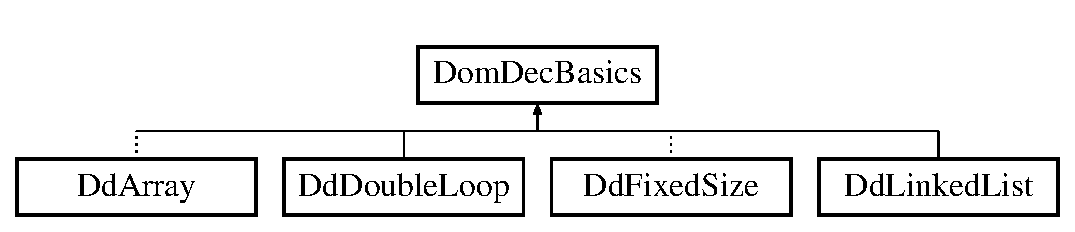
\includegraphics[height=2.000000cm]{classDomDecBasics}
\end{center}
\end{figure}
\subsubsection*{\-Public \-Member \-Functions}
\begin{DoxyCompactItemize}
\item 
\hyperlink{classDomDecBasics_aec40201a10397aa0c646f6dcb31d03d9}{\-Dom\-Dec\-Basics} ()
\begin{DoxyCompactList}\small\item\em \-Allocate. \end{DoxyCompactList}\item 
void \hyperlink{classDomDecBasics_a013bde7a8eb6c66e70ab5d90959af2c2}{\-Sig\-Err} (int \-Condition, const char $\ast$s,...)
\begin{DoxyCompactList}\small\item\em \-Handle errors. \end{DoxyCompactList}\item 
\hypertarget{classDomDecBasics_ad10ce7d8491ba213cdbc79d4dd4dc013}{int \hyperlink{classDomDecBasics_ad10ce7d8491ba213cdbc79d4dd4dc013}{\-Pos\-Ret} (const double \-Pos\mbox{[}3\mbox{]})}\label{classDomDecBasics_ad10ce7d8491ba213cdbc79d4dd4dc013}

\begin{DoxyCompactList}\small\item\em \-Relative position in the cell. \end{DoxyCompactList}\item 
int \hyperlink{classDomDecBasics_a388622b5e7d2ad20e8ac1a8a951d655f}{p\-N\-Part} ()
\begin{DoxyCompactList}\small\item\em \# part in the class \end{DoxyCompactList}\item 
int \hyperlink{classDomDecBasics_a02631cacc3cd393a64b7e78df3734e48}{p\-N\-Cell} ()
\begin{DoxyCompactList}\small\item\em \-Print the number of cells. \end{DoxyCompactList}\item 
int \hyperlink{classDomDecBasics_a8bc667d6b3e872a9cabbb54f1eb671e8}{p\-Cella} (const double \-Pos\mbox{[}3\mbox{]})
\begin{DoxyCompactList}\small\item\em (x,y,z)-\/$>$n \end{DoxyCompactList}\item 
void \hyperlink{classDomDecBasics_a328df10e55925d98bc8ca3daa5ca4f96}{p\-Cella} (const double \-Pos\mbox{[}3\mbox{]}, int c\mbox{[}4\mbox{]})
\begin{DoxyCompactList}\small\item\em (x,y,z)-\/$>$(cx,cy,cz,c\-Tot) \end{DoxyCompactList}\item 
int \hyperlink{classDomDecBasics_a14d68ab6ae97b1ddd6c8a56ec9607f87}{\-Get\-Coor\-Numb} (double $\ast$\-Pos)
\begin{DoxyCompactList}\small\item\em \-Get the coordination number. \end{DoxyCompactList}\item 
int \hyperlink{classDomDecBasics_a99b8d5719387a53ac431da0b85694056}{\-Get\-Cell\-Coord} (int c, int \-Coord, int $\ast$\-Nei\-List)
\begin{DoxyCompactList}\small\item\em \-Get the number of the neighbouring cells for the particles close to a wall. \end{DoxyCompactList}\item 
int \hyperlink{classDomDecBasics_af2721958380b0ab29aed010a01b93ab8}{\-Get\-Cell\-Coord} (double $\ast$\-Pos, int $\ast$\-Nei\-List)
\begin{DoxyCompactList}\small\item\em \-Get the number of the neighbouring cells for the particles close to a wall. \end{DoxyCompactList}\item 
int \hyperlink{classDomDecBasics_aa02df5ddcb998bf1a8f221f1bf14e063}{\-Get\-Cell\-Ch} (int c, int $\ast$\-Nei\-List)
\begin{DoxyCompactList}\small\item\em \-Get the number of the neighbouring cells. \end{DoxyCompactList}\item 
int \hyperlink{classDomDecBasics_a1d363b247b350543ea601e5f41a405eb}{\-Get\-Cell} (double $\ast$\-Pos, int $\ast$\-Nei\-List)
\begin{DoxyCompactList}\small\item\em \-Get the number of the neighbouring cells for a ghost particle. \end{DoxyCompactList}\item 
\hypertarget{classDomDecBasics_af5188eb0e6caae79f8bf349bf2345cf2}{void \hyperlink{classDomDecBasics_af5188eb0e6caae79f8bf349bf2345cf2}{\-Print\-Cell} (const int c)}\label{classDomDecBasics_af5188eb0e6caae79f8bf349bf2345cf2}

\begin{DoxyCompactList}\small\item\em \-Print the content of a cell. \end{DoxyCompactList}\item 
\hypertarget{classDomDecBasics_a1132024d8fdd721fd6a36781d4235162}{void \hyperlink{classDomDecBasics_a1132024d8fdd721fd6a36781d4235162}{\-Print\-Cells} ()}\label{classDomDecBasics_a1132024d8fdd721fd6a36781d4235162}

\begin{DoxyCompactList}\small\item\em \-Print the the particles in the cells. \end{DoxyCompactList}\item 
\hypertarget{classDomDecBasics_abacbda4ce7eed0eee33efe489157ff81}{void \hyperlink{classDomDecBasics_abacbda4ce7eed0eee33efe489157ff81}{\-Print\-List} (const int c)}\label{classDomDecBasics_abacbda4ce7eed0eee33efe489157ff81}

\begin{DoxyCompactList}\small\item\em \-Print the the particle list in the cells. \end{DoxyCompactList}\item 
\hypertarget{classDomDecBasics_aff89725be8d743f07f318ef0c06858e1}{void \hyperlink{classDomDecBasics_aff89725be8d743f07f318ef0c06858e1}{\-Print\-Lists} ()}\label{classDomDecBasics_aff89725be8d743f07f318ef0c06858e1}

\begin{DoxyCompactList}\small\item\em \-Print the the particle list in the cells. \end{DoxyCompactList}\item 
\hypertarget{classDomDecBasics_a4e589206ab9bc4752d547111d6bba6e7}{void \hyperlink{classDomDecBasics_a4e589206ab9bc4752d547111d6bba6e7}{\-Check\-List} ()}\label{classDomDecBasics_a4e589206ab9bc4752d547111d6bba6e7}

\begin{DoxyCompactList}\small\item\em \-Check the list. \end{DoxyCompactList}\item 
\hypertarget{classDomDecBasics_ad6d4b1b657a39ed64c2c45d4706dbcc1}{void \hyperlink{classDomDecBasics_ad6d4b1b657a39ed64c2c45d4706dbcc1}{\-Check\-Nei} (int p)}\label{classDomDecBasics_ad6d4b1b657a39ed64c2c45d4706dbcc1}

\begin{DoxyCompactList}\small\item\em \-Check the neighbours. \end{DoxyCompactList}\item 
int \hyperlink{classDomDecBasics_aa1b1f1f1104d2124962ffbdec630f830}{\-Set\-Cut\-Off} (double \-Cut\-Off\-Ext)
\begin{DoxyCompactList}\small\item\em \-Set the \-Cut\-Off. \end{DoxyCompactList}\end{DoxyCompactItemize}
\subsubsection*{\-Public \-Attributes}
\begin{DoxyCompactItemize}
\item 
\hypertarget{classDomDecBasics_ae47fdfe8f7b7de2ed9a00d0109696435}{double \hyperlink{classDomDecBasics_ae47fdfe8f7b7de2ed9a00d0109696435}{\-Bound\-Cond} \mbox{[}27\mbox{]}\mbox{[}3\mbox{]}}\label{classDomDecBasics_ae47fdfe8f7b7de2ed9a00d0109696435}

\begin{DoxyCompactList}\small\item\em \-Boundary condition for the cell consider. \end{DoxyCompactList}\item 
\hypertarget{classDomDecBasics_ab8d5dea32bdd50bc532a901e60a98067}{int \hyperlink{classDomDecBasics_ab8d5dea32bdd50bc532a901e60a98067}{c\-Curr}}\label{classDomDecBasics_ab8d5dea32bdd50bc532a901e60a98067}

\begin{DoxyCompactList}\small\item\em \-Cell where the current particle sits. \end{DoxyCompactList}\item 
\hypertarget{classDomDecBasics_a3f1699016098a6e8062fb140b2833206}{int \hyperlink{classDomDecBasics_a3f1699016098a6e8062fb140b2833206}{\-Nei\-List\-Curr} \mbox{[}27\mbox{]}}\label{classDomDecBasics_a3f1699016098a6e8062fb140b2833206}

\begin{DoxyCompactList}\small\item\em \-Neighbouring list. \end{DoxyCompactList}\item 
\hypertarget{classDomDecBasics_a16f1ee8ae2cd837bc80f24b844e50575}{int \hyperlink{classDomDecBasics_a16f1ee8ae2cd837bc80f24b844e50575}{\-N\-Nei\-Curr}}\label{classDomDecBasics_a16f1ee8ae2cd837bc80f24b844e50575}

\begin{DoxyCompactList}\small\item\em \-Number of neighbouring cells. \end{DoxyCompactList}\item 
\hypertarget{classDomDecBasics_a8c4a3cbd2beb1d216432d9659a8115b9}{int \hyperlink{classDomDecBasics_a8c4a3cbd2beb1d216432d9659a8115b9}{n\-Nei\-Curr}}\label{classDomDecBasics_a8c4a3cbd2beb1d216432d9659a8115b9}

\begin{DoxyCompactList}\small\item\em \-Current number of neighbours. \end{DoxyCompactList}\item 
\hypertarget{classDomDecBasics_a25fda7e50215153ef24cfcaecd5d0fd1}{int \hyperlink{classDomDecBasics_a25fda7e50215153ef24cfcaecd5d0fd1}{p1\-Curr}}\label{classDomDecBasics_a25fda7e50215153ef24cfcaecd5d0fd1}

\begin{DoxyCompactList}\small\item\em \-Reference particle. \end{DoxyCompactList}\item 
\hypertarget{classDomDecBasics_a28d65a777a97b96280ca0f9173c76c93}{int \hyperlink{classDomDecBasics_a28d65a777a97b96280ca0f9173c76c93}{p2\-Curr}}\label{classDomDecBasics_a28d65a777a97b96280ca0f9173c76c93}

\begin{DoxyCompactList}\small\item\em \-Current particle. \end{DoxyCompactList}\item 
\hypertarget{classDomDecBasics_aba0b8638ff017c1b638a2a09182e98cd}{int \hyperlink{classDomDecBasics_aba0b8638ff017c1b638a2a09182e98cd}{\-If\-Loop\-Curr}}\label{classDomDecBasics_aba0b8638ff017c1b638a2a09182e98cd}

\begin{DoxyCompactList}\small\item\em 1 if the loop is over \end{DoxyCompactList}\item 
\hypertarget{classDomDecBasics_acc8f741b84a798988735ff527e5856e2}{int \hyperlink{classDomDecBasics_acc8f741b84a798988735ff527e5856e2}{\-Mod10} \mbox{[}3\mbox{]}}\label{classDomDecBasics_acc8f741b84a798988735ff527e5856e2}

\begin{DoxyCompactList}\small\item\em \-Module 10 (nx,ny,nz) -\/$>$ nc. \end{DoxyCompactList}\item 
\hypertarget{classDomDecBasics_a8bf073be6a33b33896fcbfabfc299fb1}{int \hyperlink{classDomDecBasics_a8bf073be6a33b33896fcbfabfc299fb1}{\-N\-Cell}}\label{classDomDecBasics_a8bf073be6a33b33896fcbfabfc299fb1}

\begin{DoxyCompactList}\small\item\em \-Number of cells. \end{DoxyCompactList}\item 
\hypertarget{classDomDecBasics_aa908349bcd29a565cd53bfea2899b81e}{int \hyperlink{classDomDecBasics_aa908349bcd29a565cd53bfea2899b81e}{\-N\-Sect} \mbox{[}3\mbox{]}}\label{classDomDecBasics_aa908349bcd29a565cd53bfea2899b81e}

\begin{DoxyCompactList}\small\item\em \-Number of cells per direction. \end{DoxyCompactList}\item 
\hypertarget{classDomDecBasics_a8895c89605e91c6cf7430bad336f77c6}{double \hyperlink{classDomDecBasics_a8895c89605e91c6cf7430bad336f77c6}{\-Edge} \mbox{[}3\mbox{]}}\label{classDomDecBasics_a8895c89605e91c6cf7430bad336f77c6}

\begin{DoxyCompactList}\small\item\em \-Box sizes. \end{DoxyCompactList}\item 
\hypertarget{classDomDecBasics_a6ee15bbdebce69774ca6b655a1828b20}{double \hyperlink{classDomDecBasics_a6ee15bbdebce69774ca6b655a1828b20}{\-Inv\-Edge} \mbox{[}3\mbox{]}}\label{classDomDecBasics_a6ee15bbdebce69774ca6b655a1828b20}

\begin{DoxyCompactList}\small\item\em \-Inverse box size. \end{DoxyCompactList}\item 
\hypertarget{classDomDecBasics_af2411aba2dd63fa22b1bc279653ff7a0}{double \hyperlink{classDomDecBasics_af2411aba2dd63fa22b1bc279653ff7a0}{\-Cut\-Off}}\label{classDomDecBasics_af2411aba2dd63fa22b1bc279653ff7a0}

\begin{DoxyCompactList}\small\item\em \-Cell \-Cut\-Off. \end{DoxyCompactList}\item 
\hypertarget{classDomDecBasics_a8d8ef8940cfe4b3b94a2ffd97aaeecb3}{double \hyperlink{classDomDecBasics_a8d8ef8940cfe4b3b94a2ffd97aaeecb3}{\-Pos\-Curr} \mbox{[}3\mbox{]}}\label{classDomDecBasics_a8d8ef8940cfe4b3b94a2ffd97aaeecb3}

\begin{DoxyCompactList}\small\item\em \-Position of the current particle. \end{DoxyCompactList}\item 
\hypertarget{classDomDecBasics_a4c6eee002f7cf6e171979efae96f56d9}{int \hyperlink{classDomDecBasics_a4c6eee002f7cf6e171979efae96f56d9}{\-N\-Alloc\-P}}\label{classDomDecBasics_a4c6eee002f7cf6e171979efae96f56d9}

\begin{DoxyCompactList}\small\item\em \-Number of allocated part. \end{DoxyCompactList}\item 
\hypertarget{classDomDecBasics_abdcc792391d8c5092471dff191de47f4}{int \hyperlink{classDomDecBasics_abdcc792391d8c5092471dff191de47f4}{\-N\-Part}}\label{classDomDecBasics_abdcc792391d8c5092471dff191de47f4}

\begin{DoxyCompactList}\small\item\em \-Total number of particle. \end{DoxyCompactList}\item 
\hypertarget{classDomDecBasics_a344d1f69bf058351f6cbcc32f14a3057}{int \hyperlink{classDomDecBasics_a344d1f69bf058351f6cbcc32f14a3057}{\-N\-Neighbour}}\label{classDomDecBasics_a344d1f69bf058351f6cbcc32f14a3057}

\begin{DoxyCompactList}\small\item\em \-Number of neighbours. \end{DoxyCompactList}\end{DoxyCompactItemize}


\subsubsection{\-Detailed \-Description}
\-All the general functions shared among the different domain decomposition structures. 

\-Definition at line 35 of file \-Cubo.\-h.



\subsubsection{\-Constructor \& \-Destructor \-Documentation}
\hypertarget{classDomDecBasics_aec40201a10397aa0c646f6dcb31d03d9}{\index{\-Dom\-Dec\-Basics@{\-Dom\-Dec\-Basics}!\-Dom\-Dec\-Basics@{\-Dom\-Dec\-Basics}}
\index{\-Dom\-Dec\-Basics@{\-Dom\-Dec\-Basics}!DomDecBasics@{\-Dom\-Dec\-Basics}}
\paragraph[{\-Dom\-Dec\-Basics}]{\setlength{\rightskip}{0pt plus 5cm}{\bf \-Dom\-Dec\-Basics} (
\begin{DoxyParamCaption}
{}
\end{DoxyParamCaption}
)}}\label{classDomDecBasics_aec40201a10397aa0c646f6dcb31d03d9}


\-Allocate. 

\-Allocator of the general structure. 

\-Definition at line 17 of file \-Cubo.\-cpp.



\subsubsection{\-Member \-Function \-Documentation}
\hypertarget{classDomDecBasics_a013bde7a8eb6c66e70ab5d90959af2c2}{\index{\-Dom\-Dec\-Basics@{\-Dom\-Dec\-Basics}!\-Sig\-Err@{\-Sig\-Err}}
\index{\-Sig\-Err@{\-Sig\-Err}!DomDecBasics@{\-Dom\-Dec\-Basics}}
\paragraph[{\-Sig\-Err}]{\setlength{\rightskip}{0pt plus 5cm}void {\bf \-Sig\-Err} (
\begin{DoxyParamCaption}
\item[{int}]{\-Condition, }
\item[{const char $\ast$}]{s, }
\item[{}]{...}
\end{DoxyParamCaption}
)}}\label{classDomDecBasics_a013bde7a8eb6c66e70ab5d90959af2c2}


\-Handle errors. 

\-Signal an error and exit. 

\-Definition at line 24 of file \-Cubo.\-cpp.



\-Referenced by \-Dd\-Linked\-List\-::\-Add\-Part(), \-Dd\-Linked\-List\-::\-Couple(), \-Dd\-Double\-Loop\-::\-Dd\-Double\-Loop(), \-Dd\-Linked\-List\-::\-Dd\-Linked\-List(), \-Get\-Cell\-Ch(), \-Get\-Cell\-Coord(), \-Dd\-Linked\-List\-::\-Incr\-Curr\-List(), \-Dd\-Linked\-List\-::\-It\-Cell(), p\-Cella(), \-Dd\-Linked\-List\-::\-Rem\-Part(), \-Dd\-Linked\-List\-::\-Set\-Curr(), and \-Dd\-Linked\-List\-::\-Set\-Curr\-Ghost().

\hypertarget{classDomDecBasics_a388622b5e7d2ad20e8ac1a8a951d655f}{\index{\-Dom\-Dec\-Basics@{\-Dom\-Dec\-Basics}!p\-N\-Part@{p\-N\-Part}}
\index{p\-N\-Part@{p\-N\-Part}!DomDecBasics@{\-Dom\-Dec\-Basics}}
\paragraph[{p\-N\-Part}]{\setlength{\rightskip}{0pt plus 5cm}int {\bf p\-N\-Part} (
\begin{DoxyParamCaption}
{}
\end{DoxyParamCaption}
)}}\label{classDomDecBasics_a388622b5e7d2ad20e8ac1a8a951d655f}


\# part in the class 

\-Number of particles. 

\-Reimplemented in \hyperlink{classDdDoubleLoop_a388622b5e7d2ad20e8ac1a8a951d655f}{\-Dd\-Double\-Loop}, and \hyperlink{classDdLinkedList_a388622b5e7d2ad20e8ac1a8a951d655f}{\-Dd\-Linked\-List}.



\-Definition at line 51 of file \-Cubo.\-cpp.



\-References \-N\-Part.

\hypertarget{classDomDecBasics_a02631cacc3cd393a64b7e78df3734e48}{\index{\-Dom\-Dec\-Basics@{\-Dom\-Dec\-Basics}!p\-N\-Cell@{p\-N\-Cell}}
\index{p\-N\-Cell@{p\-N\-Cell}!DomDecBasics@{\-Dom\-Dec\-Basics}}
\paragraph[{p\-N\-Cell}]{\setlength{\rightskip}{0pt plus 5cm}int {\bf p\-N\-Cell} (
\begin{DoxyParamCaption}
{}
\end{DoxyParamCaption}
)}}\label{classDomDecBasics_a02631cacc3cd393a64b7e78df3734e48}


\-Print the number of cells. 

\-Number of cells. 

\-Reimplemented in \hyperlink{classDdArray_a02631cacc3cd393a64b7e78df3734e48}{\-Dd\-Array}.



\-Definition at line 55 of file \-Cubo.\-cpp.



\-References \-N\-Cell.

\hypertarget{classDomDecBasics_a8bc667d6b3e872a9cabbb54f1eb671e8}{\index{\-Dom\-Dec\-Basics@{\-Dom\-Dec\-Basics}!p\-Cella@{p\-Cella}}
\index{p\-Cella@{p\-Cella}!DomDecBasics@{\-Dom\-Dec\-Basics}}
\paragraph[{p\-Cella}]{\setlength{\rightskip}{0pt plus 5cm}int {\bf p\-Cella} (
\begin{DoxyParamCaption}
\item[{const double}]{\-Pos\mbox{[}3\mbox{]}}
\end{DoxyParamCaption}
)}}\label{classDomDecBasics_a8bc667d6b3e872a9cabbb54f1eb671e8}


(x,y,z)-\/$>$n 

\-Return the unique cell identification number for the given position. 

\-Definition at line 192 of file \-Cubo.\-cpp.



\-References \-Edge, \-Inv\-Edge, \-Mod10, \-N\-Cell, \-N\-Sect, and \-Sig\-Err().



\-Referenced by \-Dd\-Linked\-List\-::\-Add\-Part(), \-Dd\-Array\-::\-Add\-Part(), \-Dd\-Fixed\-Size\-::\-Add\-Part(), \-Get\-Cell(), \-Get\-Cell\-Coord(), \-Dd\-Linked\-List\-::\-Move\-Part(), \-Dd\-Array\-::\-Move\-Part(), \-Dd\-Fixed\-Size\-::\-Move\-Part(), \-Dd\-Linked\-List\-::\-Rem\-Part(), \-Dd\-Array\-::\-Rem\-Part(), \-Dd\-Fixed\-Size\-::\-Rem\-Part(), \-Dd\-Linked\-List\-::\-Set\-Curr\-Ghost(), \-Dd\-Array\-::\-Swap\-Part(), and \-Dd\-Fixed\-Size\-::\-Swap\-Part().

\hypertarget{classDomDecBasics_a328df10e55925d98bc8ca3daa5ca4f96}{\index{\-Dom\-Dec\-Basics@{\-Dom\-Dec\-Basics}!p\-Cella@{p\-Cella}}
\index{p\-Cella@{p\-Cella}!DomDecBasics@{\-Dom\-Dec\-Basics}}
\paragraph[{p\-Cella}]{\setlength{\rightskip}{0pt plus 5cm}void {\bf p\-Cella} (
\begin{DoxyParamCaption}
\item[{const double}]{\-Pos\mbox{[}3\mbox{]}, }
\item[{int}]{c\mbox{[}4\mbox{]}}
\end{DoxyParamCaption}
)}}\label{classDomDecBasics_a328df10e55925d98bc8ca3daa5ca4f96}


(x,y,z)-\/$>$(cx,cy,cz,c\-Tot) 

\-Return the unique cell identification number for the given position. 

\-Definition at line 203 of file \-Cubo.\-cpp.



\-References \-Edge, \-Mod10, \-N\-Cell, \-N\-Sect, and \-Sig\-Err().

\hypertarget{classDomDecBasics_a14d68ab6ae97b1ddd6c8a56ec9607f87}{\index{\-Dom\-Dec\-Basics@{\-Dom\-Dec\-Basics}!\-Get\-Coor\-Numb@{\-Get\-Coor\-Numb}}
\index{\-Get\-Coor\-Numb@{\-Get\-Coor\-Numb}!DomDecBasics@{\-Dom\-Dec\-Basics}}
\paragraph[{\-Get\-Coor\-Numb}]{\setlength{\rightskip}{0pt plus 5cm}int {\bf \-Get\-Coor\-Numb} (
\begin{DoxyParamCaption}
\item[{double $\ast$}]{\-Pos}
\end{DoxyParamCaption}
)}}\label{classDomDecBasics_a14d68ab6ae97b1ddd6c8a56ec9607f87}


\-Get the coordination number. 

\-Retrun the coordination number for the given position. 

\-Definition at line 212 of file \-Cubo.\-cpp.



\-References \-Cut\-Off, \-Edge, and \-N\-Sect.



\-Referenced by \-Get\-Cell\-Coord(), \-Dd\-Linked\-List\-::\-Set\-Coor\-Numb(), and \-Dd\-Double\-Loop\-::\-Set\-Coor\-Numb().

\hypertarget{classDomDecBasics_a99b8d5719387a53ac431da0b85694056}{\index{\-Dom\-Dec\-Basics@{\-Dom\-Dec\-Basics}!\-Get\-Cell\-Coord@{\-Get\-Cell\-Coord}}
\index{\-Get\-Cell\-Coord@{\-Get\-Cell\-Coord}!DomDecBasics@{\-Dom\-Dec\-Basics}}
\paragraph[{\-Get\-Cell\-Coord}]{\setlength{\rightskip}{0pt plus 5cm}int {\bf \-Get\-Cell\-Coord} (
\begin{DoxyParamCaption}
\item[{int}]{c, }
\item[{int}]{\-Coord, }
\item[{int $\ast$}]{\-Nei\-List}
\end{DoxyParamCaption}
)}}\label{classDomDecBasics_a99b8d5719387a53ac431da0b85694056}


\-Get the number of the neighbouring cells for the particles close to a wall. 

\-Coordination number of the particle in the cell, every particle has a flag which tells to which cell border is close to.

\-Saves computational time. 

\-Definition at line 121 of file \-Cubo.\-cpp.



\-References \-Bound\-Cond, \-Mod10, \-N\-Sect, and \-Sig\-Err().



\-Referenced by \-Get\-Cell\-Coord().

\hypertarget{classDomDecBasics_af2721958380b0ab29aed010a01b93ab8}{\index{\-Dom\-Dec\-Basics@{\-Dom\-Dec\-Basics}!\-Get\-Cell\-Coord@{\-Get\-Cell\-Coord}}
\index{\-Get\-Cell\-Coord@{\-Get\-Cell\-Coord}!DomDecBasics@{\-Dom\-Dec\-Basics}}
\paragraph[{\-Get\-Cell\-Coord}]{\setlength{\rightskip}{0pt plus 5cm}int {\bf \-Get\-Cell\-Coord} (
\begin{DoxyParamCaption}
\item[{double $\ast$}]{\-Pos, }
\item[{int $\ast$}]{\-Nei\-List}
\end{DoxyParamCaption}
)}}\label{classDomDecBasics_af2721958380b0ab29aed010a01b93ab8}


\-Get the number of the neighbouring cells for the particles close to a wall. 

\-Coordination number of the particle in the cell. 

\-Definition at line 115 of file \-Cubo.\-cpp.



\-References \-Get\-Cell\-Coord(), \-Get\-Coor\-Numb(), and p\-Cella().

\hypertarget{classDomDecBasics_aa02df5ddcb998bf1a8f221f1bf14e063}{\index{\-Dom\-Dec\-Basics@{\-Dom\-Dec\-Basics}!\-Get\-Cell\-Ch@{\-Get\-Cell\-Ch}}
\index{\-Get\-Cell\-Ch@{\-Get\-Cell\-Ch}!DomDecBasics@{\-Dom\-Dec\-Basics}}
\paragraph[{\-Get\-Cell\-Ch}]{\setlength{\rightskip}{0pt plus 5cm}int {\bf \-Get\-Cell\-Ch} (
\begin{DoxyParamCaption}
\item[{int}]{c, }
\item[{int $\ast$}]{\-Nei\-List}
\end{DoxyParamCaption}
)}}\label{classDomDecBasics_aa02df5ddcb998bf1a8f221f1bf14e063}


\-Get the number of the neighbouring cells. 

\-Neighbouring cells with periodic boundary conditions. 

\-Definition at line 64 of file \-Cubo.\-cpp.



\-References \-Bound\-Cond, \-Mod10, \-N\-Cell, \-N\-Sect, and \-Sig\-Err().



\-Referenced by \-Get\-Cell().

\hypertarget{classDomDecBasics_a1d363b247b350543ea601e5f41a405eb}{\index{\-Dom\-Dec\-Basics@{\-Dom\-Dec\-Basics}!\-Get\-Cell@{\-Get\-Cell}}
\index{\-Get\-Cell@{\-Get\-Cell}!DomDecBasics@{\-Dom\-Dec\-Basics}}
\paragraph[{\-Get\-Cell}]{\setlength{\rightskip}{0pt plus 5cm}int {\bf \-Get\-Cell} (
\begin{DoxyParamCaption}
\item[{double $\ast$}]{\-Pos, }
\item[{int $\ast$}]{\-Nei\-List}
\end{DoxyParamCaption}
)}}\label{classDomDecBasics_a1d363b247b350543ea601e5f41a405eb}


\-Get the number of the neighbouring cells for a ghost particle. 

\-Return the list of neighbouring cells. 

\-Definition at line 59 of file \-Cubo.\-cpp.



\-References \-Get\-Cell\-Ch(), and p\-Cella().

\hypertarget{classDomDecBasics_aa1b1f1f1104d2124962ffbdec630f830}{\index{\-Dom\-Dec\-Basics@{\-Dom\-Dec\-Basics}!\-Set\-Cut\-Off@{\-Set\-Cut\-Off}}
\index{\-Set\-Cut\-Off@{\-Set\-Cut\-Off}!DomDecBasics@{\-Dom\-Dec\-Basics}}
\paragraph[{\-Set\-Cut\-Off}]{\setlength{\rightskip}{0pt plus 5cm}int {\bf \-Set\-Cut\-Off} (
\begin{DoxyParamCaption}
\item[{double}]{\-Cut\-Off\-Ext}
\end{DoxyParamCaption}
)}}\label{classDomDecBasics_aa1b1f1f1104d2124962ffbdec630f830}


\-Set the \-Cut\-Off. 

\-Set the cut off of the grid spacing, the cut off should be much smaller than the box size. 

\-Definition at line 40 of file \-Cubo.\-cpp.



\-References \-Cut\-Off, \-Edge, and \-N\-Sect.



\-Referenced by \-Dd\-Double\-Loop\-::\-Dd\-Double\-Loop(), and \-Dd\-Linked\-List\-::\-Dd\-Linked\-List().



\-The documentation for this class was generated from the following files\-:\begin{DoxyCompactItemize}
\item 
include/\-Cubo.\-h\item 
src/\-Var\-Data/\-Cubo.\-cpp\item 
src/\-Var\-Data/\-Cubo.\-mirror.\-cpp\end{DoxyCompactItemize}

\hypertarget{classDomPart}{}\subsection{Dom\+Part Class Reference}
\label{classDomPart}\index{Dom\+Part@{Dom\+Part}}


The previuos and consecutive particle in the cell linked list.  




{\ttfamily \#include $<$Cubo.\+h$>$}

\subsubsection*{Public Member Functions}
\begin{DoxyCompactItemize}
\item 
{\bfseries Dom\+Part} (int N\+Part)\hypertarget{classDomPart_ab2a1821c2ce0c7963f55101016fb438d}{}\label{classDomPart_ab2a1821c2ce0c7963f55101016fb438d}

\item 
int \hyperlink{classDomPart_a72c73510fb6bfedfb82d906895bdaf07}{operator\mbox{[}$\,$\mbox{]}} (int col)\hypertarget{classDomPart_a72c73510fb6bfedfb82d906895bdaf07}{}\label{classDomPart_a72c73510fb6bfedfb82d906895bdaf07}

\begin{DoxyCompactList}\small\item\em Returns a entry. \end{DoxyCompactList}\item 
\hyperlink{classDomPart}{Dom\+Part} \& \hyperlink{classDomPart_a580c80d8a662e0f4c16d04778d140dda}{operator++} ()\hypertarget{classDomPart_a580c80d8a662e0f4c16d04778d140dda}{}\label{classDomPart_a580c80d8a662e0f4c16d04778d140dda}

\begin{DoxyCompactList}\small\item\em Increase the iterator, deactivated. \end{DoxyCompactList}\end{DoxyCompactItemize}


\subsubsection{Detailed Description}
The previuos and consecutive particle in the cell linked list. 

Definition at line 114 of file Cubo.\+h.



The documentation for this class was generated from the following files\+:\begin{DoxyCompactItemize}
\item 
include/Cubo.\+h\item 
src/\+Var\+Data/Cubo.\+cpp\item 
src/\+Var\+Data/Cubo.\+mirror.\+cpp\end{DoxyCompactItemize}

\hypertarget{classDraw}{\subsection{\-Draw \-Class \-Reference}
\label{classDraw}\index{\-Draw@{\-Draw}}
}


\hyperlink{classDraw}{\-Draw} provides the basic configuration of the open\-G\-L libraries used in every derived program.  




{\ttfamily \#include $<$\-Draw.\-h$>$}

\-Inheritance diagram for \-Draw\-:\begin{figure}[H]
\begin{center}
\leavevmode
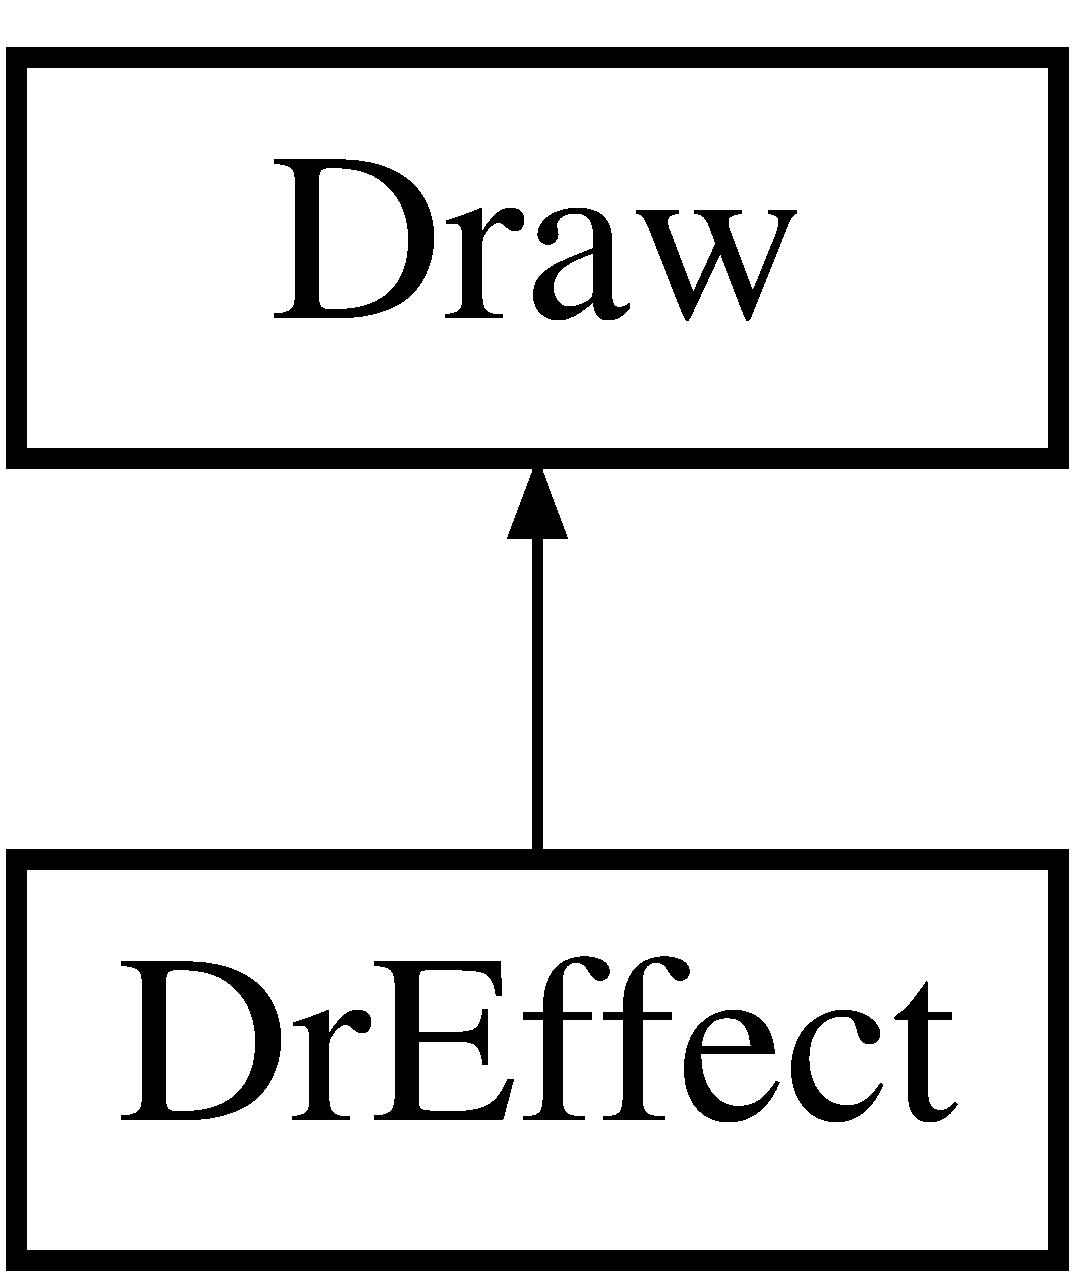
\includegraphics[height=2.000000cm]{classDraw}
\end{center}
\end{figure}
\subsubsection*{\-Public \-Types}
\begin{DoxyCompactItemize}
\item 
\hypertarget{classDraw_af1513ca0f3e04442fc69e97a85ade56e}{typedef void(\-Draw\-::$\ast$ \hyperlink{classDraw_af1513ca0f3e04442fc69e97a85ade56e}{\-D\-E\-P\-T\-H\-\_\-\-M\-A\-P} )(double \-Val, \-G\-Lfloat $\ast$\-Color)}\label{classDraw_af1513ca0f3e04442fc69e97a85ade56e}

\begin{DoxyCompactList}\small\item\em \-Data type for distance/field functions. \end{DoxyCompactList}\end{DoxyCompactItemize}
\subsubsection*{\-Public \-Member \-Functions}
\begin{DoxyCompactItemize}
\item 
\hypertarget{classDraw_a6d1a6c1ede3d0e58cbf0534c9c3ba943}{void \hyperlink{classDraw_a6d1a6c1ede3d0e58cbf0534c9c3ba943}{\-Draw1} (void)}\label{classDraw_a6d1a6c1ede3d0e58cbf0534c9c3ba943}

\begin{DoxyCompactList}\small\item\em \-A scene for debugging. \end{DoxyCompactList}\item 
\hypertarget{classDraw_a13a208315366febdc9db2eefb5f354ab}{void \hyperlink{classDraw_a13a208315366febdc9db2eefb5f354ab}{\-D\-Minimal} (void)}\label{classDraw_a13a208315366febdc9db2eefb5f354ab}

\begin{DoxyCompactList}\small\item\em \-A empty scene (only the list) \end{DoxyCompactList}\item 
\hypertarget{classDraw_a4d4cb243d25c9778b824719fc01d8b68}{void \hyperlink{classDraw_a4d4cb243d25c9778b824719fc01d8b68}{\-Dr\-Triangles} (int \-N\-Point)}\label{classDraw_a4d4cb243d25c9778b824719fc01d8b68}

\begin{DoxyCompactList}\small\item\em \-Boh. \end{DoxyCompactList}\item 
\hypertarget{classDraw_aded17e5e58c8d26011c3d2120b259fed}{void \hyperlink{classDraw_aded17e5e58c8d26011c3d2120b259fed}{\-Show\-Image} ()}\label{classDraw_aded17e5e58c8d26011c3d2120b259fed}

\begin{DoxyCompactList}\small\item\em \-Displays the data stored in pixel. \end{DoxyCompactList}\item 
\hypertarget{classDraw_a6768324ebecaa6d87d6e65bf242b23f9}{void \hyperlink{classDraw_a6768324ebecaa6d87d6e65bf242b23f9}{\-Window} (int argc, char $\ast$$\ast$argv)}\label{classDraw_a6768324ebecaa6d87d6e65bf242b23f9}

\begin{DoxyCompactList}\small\item\em \-Initial definition of the window. \end{DoxyCompactList}\item 
\hypertarget{classDraw_aa74f5eca0e42920b3ae0766299b85617}{void \hyperlink{classDraw_aa74f5eca0e42920b3ae0766299b85617}{\-D\-Figure} (void)}\label{classDraw_aa74f5eca0e42920b3ae0766299b85617}

\begin{DoxyCompactList}\small\item\em \-Definition of the scene on which the objects will be drawn. \end{DoxyCompactList}\item 
\hypertarget{classDraw_a3c4f3df21652856a8394a447d2afa61d}{void \hyperlink{classDraw_a3c4f3df21652856a8394a447d2afa61d}{\-D\-Timer} (int v)}\label{classDraw_a3c4f3df21652856a8394a447d2afa61d}

\begin{DoxyCompactList}\small\item\em \-Not working. \end{DoxyCompactList}\item 
\hypertarget{classDraw_a0cd7542f249d2cef85422d5ae63de96a}{void \hyperlink{classDraw_a0cd7542f249d2cef85422d5ae63de96a}{\-Dreshape} (int w, int h)}\label{classDraw_a0cd7542f249d2cef85422d5ae63de96a}

\begin{DoxyCompactList}\small\item\em \-Principal reshape function. \end{DoxyCompactList}\item 
\hypertarget{classDraw_a109d40d540116a12e8fe6b88dcd1ec89}{int \hyperlink{classDraw_a109d40d540116a12e8fe6b88dcd1ec89}{\-Apply\-Texture} ()}\label{classDraw_a109d40d540116a12e8fe6b88dcd1ec89}

\begin{DoxyCompactList}\small\item\em \-Apply the texture to a square. \end{DoxyCompactList}\item 
\hypertarget{classDraw_ab319e761c351a70537cda32d33f63098}{int \hyperlink{classDraw_ab319e761c351a70537cda32d33f63098}{\-Show\-Texture} ()}\label{classDraw_ab319e761c351a70537cda32d33f63098}

\begin{DoxyCompactList}\small\item\em \-Call the texture in the scene. \end{DoxyCompactList}\item 
\hypertarget{classDraw_a26cd1ca797b17da835a5d2050c6dda2f}{void \hyperlink{classDraw_a26cd1ca797b17da835a5d2050c6dda2f}{\-Transform} ()}\label{classDraw_a26cd1ca797b17da835a5d2050c6dda2f}

\begin{DoxyCompactList}\small\item\em \-Transform the system coordinates. \end{DoxyCompactList}\item 
\hypertarget{classDraw_ae391a0fc7ddb11d90732dd74249f5fe7}{void \hyperlink{classDraw_ae391a0fc7ddb11d90732dd74249f5fe7}{\-Dr\-Cube} ()}\label{classDraw_ae391a0fc7ddb11d90732dd74249f5fe7}

\begin{DoxyCompactList}\small\item\em \-Line in a cube. \end{DoxyCompactList}\item 
\hypertarget{classDraw_affbc65c5c21480f96c44a3a007eab346}{void \hyperlink{classDraw_affbc65c5c21480f96c44a3a007eab346}{\-Choose\-Blend} (int \-Which)}\label{classDraw_affbc65c5c21480f96c44a3a007eab346}

\begin{DoxyCompactList}\small\item\em \-Choose a different blending function. \end{DoxyCompactList}\item 
\hypertarget{classDraw_a54d1e606bdbeb32edce52a58531b9a1c}{void \hyperlink{classDraw_a54d1e606bdbeb32edce52a58531b9a1c}{\-Put\-String} (double $\ast$\-Pos, char $\ast$\-String)}\label{classDraw_a54d1e606bdbeb32edce52a58531b9a1c}

\begin{DoxyCompactList}\small\item\em \-Put a string. \end{DoxyCompactList}\item 
\hypertarget{classDraw_af8297bf0b592efa35fb5b8e62ecf9c29}{void \hyperlink{classDraw_af8297bf0b592efa35fb5b8e62ecf9c29}{\-Put\-String} (double \-Posx, double \-Posy, double \-Posz, char $\ast$\-String)}\label{classDraw_af8297bf0b592efa35fb5b8e62ecf9c29}

\begin{DoxyCompactList}\small\item\em \-Put a string. \end{DoxyCompactList}\item 
void \hyperlink{classDraw_a7a0fab2975ffd1787c0d9168f5a8574c}{\-Numera} (double $\ast$\-Pos, int n)
\begin{DoxyCompactList}\small\item\em \-Print the. \end{DoxyCompactList}\item 
\hypertarget{classDraw_ac5e4238325fb9dde3862a6f1053b5e8d}{void \hyperlink{classDraw_ac5e4238325fb9dde3862a6f1053b5e8d}{\-Lista} (int \-N\-Square)}\label{classDraw_ac5e4238325fb9dde3862a6f1053b5e8d}

\begin{DoxyCompactList}\small\item\em \-Definition of the primitives. \end{DoxyCompactList}\item 
\hypertarget{classDraw_a318bab761ab1ad340c3a7d2d17df4f9b}{int \hyperlink{classDraw_a318bab761ab1ad340c3a7d2d17df4f9b}{\-Def\-Point} ()}\label{classDraw_a318bab761ab1ad340c3a7d2d17df4f9b}

\begin{DoxyCompactList}\small\item\em \-Point. \end{DoxyCompactList}\item 
\hypertarget{classDraw_a0ab1b8899eb5e75e63634120f152d532}{int \hyperlink{classDraw_a0ab1b8899eb5e75e63634120f152d532}{\-Def\-Cube} (int \-N\-Square)}\label{classDraw_a0ab1b8899eb5e75e63634120f152d532}

\begin{DoxyCompactList}\small\item\em \-Cube. \end{DoxyCompactList}\item 
\hypertarget{classDraw_a7e12d94e8036fd5222db58072fe8a4c1}{int \hyperlink{classDraw_a7e12d94e8036fd5222db58072fe8a4c1}{\-Def\-Quad} (int \-N\-Square)}\label{classDraw_a7e12d94e8036fd5222db58072fe8a4c1}

\begin{DoxyCompactList}\small\item\em \-Quad. \end{DoxyCompactList}\item 
\hypertarget{classDraw_af4ca54f4f60c7e6b3e44f81a82afa810}{int \hyperlink{classDraw_af4ca54f4f60c7e6b3e44f81a82afa810}{\-Def\-Cylinder} (double \-Rad, double \-Height)}\label{classDraw_af4ca54f4f60c7e6b3e44f81a82afa810}

\begin{DoxyCompactList}\small\item\em \-Cylinder. \end{DoxyCompactList}\item 
\hypertarget{classDraw_a48bd0a016aeca0bc3c42ddfbe4597bdc}{int \hyperlink{classDraw_a48bd0a016aeca0bc3c42ddfbe4597bdc}{\-Def\-Metal\-Cylinder} (double \-Rad, double \-Height)}\label{classDraw_a48bd0a016aeca0bc3c42ddfbe4597bdc}

\begin{DoxyCompactList}\small\item\em \-Metallic cylinder. \end{DoxyCompactList}\item 
\hypertarget{classDraw_a57d5c994950e11fb7e58680393213343}{int \hyperlink{classDraw_a57d5c994950e11fb7e58680393213343}{\-Def\-Hexagon} ()}\label{classDraw_a57d5c994950e11fb7e58680393213343}

\begin{DoxyCompactList}\small\item\em \-Hexagon. \end{DoxyCompactList}\item 
\hypertarget{classDraw_adec17f3a83b10efe43dee2808cc57194}{int \hyperlink{classDraw_adec17f3a83b10efe43dee2808cc57194}{\-Def\-Griglia} ()}\label{classDraw_adec17f3a83b10efe43dee2808cc57194}

\begin{DoxyCompactList}\small\item\em \-Griglia. \end{DoxyCompactList}\item 
\hypertarget{classDraw_a9e8807139062d3d8e7a5ae14e98480da}{int \hyperlink{classDraw_a9e8807139062d3d8e7a5ae14e98480da}{\-Def\-Wall} ()}\label{classDraw_a9e8807139062d3d8e7a5ae14e98480da}

\begin{DoxyCompactList}\small\item\em \-Wall. \end{DoxyCompactList}\item 
\hypertarget{classDraw_aa63c0ecef2860e57c23d6ff1e631189b}{int \hyperlink{classDraw_aa63c0ecef2860e57c23d6ff1e631189b}{\-Def\-Arrow} ()}\label{classDraw_aa63c0ecef2860e57c23d6ff1e631189b}

\begin{DoxyCompactList}\small\item\em \-Arrow. \end{DoxyCompactList}\item 
\hypertarget{classDraw_a19a76422b4564ec10df73ec0256f2974}{int \hyperlink{classDraw_a19a76422b4564ec10df73ec0256f2974}{\-Def\-Arrow\-Thin} ()}\label{classDraw_a19a76422b4564ec10df73ec0256f2974}

\begin{DoxyCompactList}\small\item\em \-Arrow. \end{DoxyCompactList}\item 
\hypertarget{classDraw_a5fd96ad8c1ebeede7341bcf3a20aa65d}{int \hyperlink{classDraw_a5fd96ad8c1ebeede7341bcf3a20aa65d}{\-Def\-Texture} ()}\label{classDraw_a5fd96ad8c1ebeede7341bcf3a20aa65d}

\begin{DoxyCompactList}\small\item\em \-Define a simple texture. \end{DoxyCompactList}\item 
\hypertarget{classDraw_ac0790850f6751e5fe0f47d16d7f67255}{void \hyperlink{classDraw_ac0790850f6751e5fe0f47d16d7f67255}{\-Init\-Constant} ()}\label{classDraw_ac0790850f6751e5fe0f47d16d7f67255}

\begin{DoxyCompactList}\small\item\em \-Initializes all the view constants. \end{DoxyCompactList}\item 
\hypertarget{classDraw_a16f350a8340f724d1b358e89fe18c340}{double \hyperlink{classDraw_a16f350a8340f724d1b358e89fe18c340}{\-Normal} (double $\ast$v, double $\ast$u, double $\ast$w, double $\ast$n)}\label{classDraw_a16f350a8340f724d1b358e89fe18c340}

\begin{DoxyCompactList}\small\item\em \-Calculate the normal. \end{DoxyCompactList}\item 
\hypertarget{classDraw_ab3d9c36aceb9e5f4b158eb15b47c2003}{void \hyperlink{classDraw_ab3d9c36aceb9e5f4b158eb15b47c2003}{\-Depth\-Map} (double \-Val, \-G\-Lfloat $\ast$\-Color)}\label{classDraw_ab3d9c36aceb9e5f4b158eb15b47c2003}

\begin{DoxyCompactList}\small\item\em \-Pointer to a generic function. \end{DoxyCompactList}\item 
\hypertarget{classDraw_a6c0ca0bd4c1c0efc555672b6671535bc}{void \hyperlink{classDraw_a6c0ca0bd4c1c0efc555672b6671535bc}{\-Depth\-Map1} (double \-Val, \-G\-Lfloat $\ast$\-Color)}\label{classDraw_a6c0ca0bd4c1c0efc555672b6671535bc}

\begin{DoxyCompactList}\small\item\em \-Depth map. \end{DoxyCompactList}\item 
\hypertarget{classDraw_af5edc3c8867513cbb290646b3e0e20ff}{void \hyperlink{classDraw_af5edc3c8867513cbb290646b3e0e20ff}{\-Choose\-Depth\-Map} (int n)}\label{classDraw_af5edc3c8867513cbb290646b3e0e20ff}

\begin{DoxyCompactList}\small\item\em \-Choose \-Depth map. \end{DoxyCompactList}\item 
\hypertarget{classDraw_a5456e2c12fe02429ecf5bc09273ac3ed}{int \hyperlink{classDraw_a5456e2c12fe02429ecf5bc09273ac3ed}{\-Def\-Legend} ()}\label{classDraw_a5456e2c12fe02429ecf5bc09273ac3ed}

\begin{DoxyCompactList}\small\item\em \-Depth map. \end{DoxyCompactList}\item 
\hypertarget{classDraw_a8332766d3980ae20e0fb7e2a290a59ea}{void \hyperlink{classDraw_a8332766d3980ae20e0fb7e2a290a59ea}{\-Dmouse} (int button, int state, int x, int y)}\label{classDraw_a8332766d3980ae20e0fb7e2a290a59ea}

\begin{DoxyCompactList}\small\item\em \-To launch the menu. \end{DoxyCompactList}\item 
\hypertarget{classDraw_a9794ec43c2f8cf4e106aad7e0c2e1b66}{void \hyperlink{classDraw_a9794ec43c2f8cf4e106aad7e0c2e1b66}{\-D\-Mouse\-Move} (int x, int y)}\label{classDraw_a9794ec43c2f8cf4e106aad7e0c2e1b66}

\begin{DoxyCompactList}\small\item\em \-How the scene rotate (\-Camera view should be implemented) \end{DoxyCompactList}\item 
\hypertarget{classDraw_ab63c111588287a2a7ccf27b480f49d06}{void \hyperlink{classDraw_ab63c111588287a2a7ccf27b480f49d06}{\-Dspecial} (int k, int x, int y)}\label{classDraw_ab63c111588287a2a7ccf27b480f49d06}

\begin{DoxyCompactList}\small\item\em \-Boh. \end{DoxyCompactList}\item 
\hypertarget{classDraw_a60d9d96dd62e71bfe22654f9d58f834b}{void \hyperlink{classDraw_a60d9d96dd62e71bfe22654f9d58f834b}{keyboard\-Draw} (unsigned char key)}\label{classDraw_a60d9d96dd62e71bfe22654f9d58f834b}

\begin{DoxyCompactList}\small\item\em \-Combines the key with the functions. \end{DoxyCompactList}\item 
\hypertarget{classDraw_aabbfd9c8269f5409bd80617f17ee17a6}{void \hyperlink{classDraw_aabbfd9c8269f5409bd80617f17ee17a6}{\-Camera\-Quat} ()}\label{classDraw_aabbfd9c8269f5409bd80617f17ee17a6}

\begin{DoxyCompactList}\small\item\em \-Quaternion camera implementation. \end{DoxyCompactList}\item 
\hypertarget{classDraw_a62cfcd5895c1c14a27f38007fd00ef28}{void \hyperlink{classDraw_a62cfcd5895c1c14a27f38007fd00ef28}{\-Change\-Su\-Giu} (\-G\-Lfloat \-Movement)}\label{classDraw_a62cfcd5895c1c14a27f38007fd00ef28}

\begin{DoxyCompactList}\small\item\em \-Movement up-\/down. \end{DoxyCompactList}\item 
\hypertarget{classDraw_a8d619bf9e67c2d0684777837c50cd820}{void \hyperlink{classDraw_a8d619bf9e67c2d0684777837c50cd820}{\-Change\-Dx\-Sx} (\-G\-Lfloat \-Movement)}\label{classDraw_a8d619bf9e67c2d0684777837c50cd820}

\begin{DoxyCompactList}\small\item\em \-Movement right left. \end{DoxyCompactList}\item 
\hypertarget{classDraw_a7fe6a9c0c549657aa0d7da2e3c73fa01}{void \hyperlink{classDraw_a7fe6a9c0c549657aa0d7da2e3c73fa01}{abort\-\_\-} (const char $\ast$s,...)}\label{classDraw_a7fe6a9c0c549657aa0d7da2e3c73fa01}

\begin{DoxyCompactList}\small\item\em \-Check. \end{DoxyCompactList}\item 
\hypertarget{classDraw_a45ed15a0527d5ba75107645dc8467078}{int \hyperlink{classDraw_a45ed15a0527d5ba75107645dc8467078}{\-Picture} ()}\label{classDraw_a45ed15a0527d5ba75107645dc8467078}

\begin{DoxyCompactList}\small\item\em \-Write a tiff file of the data in pixel. \end{DoxyCompactList}\item 
\hypertarget{classDraw_a289d8cd3100d77331ac7879eedcfcad0}{int \hyperlink{classDraw_a289d8cd3100d77331ac7879eedcfcad0}{\-Write\-Pixel} ()}\label{classDraw_a289d8cd3100d77331ac7879eedcfcad0}

\begin{DoxyCompactList}\small\item\em \-Boh. \end{DoxyCompactList}\item 
\hypertarget{classDraw_a0b5ba668037c62f126f6d480048f9087}{int \hyperlink{classDraw_a0b5ba668037c62f126f6d480048f9087}{\-Write\-Png} ()}\label{classDraw_a0b5ba668037c62f126f6d480048f9087}

\begin{DoxyCompactList}\small\item\em \-Write a png file of the data in pixel (not working) \end{DoxyCompactList}\item 
\hypertarget{classDraw_a46f9540fd46154cbfd9669ac414dbe2a}{int \hyperlink{classDraw_a46f9540fd46154cbfd9669ac414dbe2a}{\-Write\-Pngwriter} ()}\label{classDraw_a46f9540fd46154cbfd9669ac414dbe2a}

\begin{DoxyCompactList}\small\item\em \-Write a png file of the data in pixel (uses libpngwriter) \end{DoxyCompactList}\item 
\hypertarget{classDraw_a2e01e34ba6507a931ca7535f99c26347}{int \hyperlink{classDraw_a2e01e34ba6507a931ca7535f99c26347}{\-Open\-Image} (const char $\ast$\-File\-Name)}\label{classDraw_a2e01e34ba6507a931ca7535f99c26347}

\begin{DoxyCompactList}\small\item\em \-Open a image to be store in pixel. \end{DoxyCompactList}\item 
\hypertarget{classDraw_ad84f29894ee58a4e931cdbc41ba7a9d2}{void \hyperlink{classDraw_ad84f29894ee58a4e931cdbc41ba7a9d2}{\-Read\-Script} ()}\label{classDraw_ad84f29894ee58a4e931cdbc41ba7a9d2}

\begin{DoxyCompactList}\small\item\em \-Reads and draw a script file. \end{DoxyCompactList}\item 
\hypertarget{classDraw_a6f390f3a650790d32dd2860703f57e98}{void \hyperlink{classDraw_a6f390f3a650790d32dd2860703f57e98}{\-Read\-Conf} ()}\label{classDraw_a6f390f3a650790d32dd2860703f57e98}

\begin{DoxyCompactList}\small\item\em \-Reads and applies external configurations. \end{DoxyCompactList}\end{DoxyCompactItemize}
\subsubsection*{\-Public \-Attributes}
\begin{DoxyCompactItemize}
\item 
\hypertarget{classDraw_a840dda96dc55e47741fc47e2a7c80526}{\hyperlink{classDraw_af1513ca0f3e04442fc69e97a85ade56e}{\-D\-E\-P\-T\-H\-\_\-\-M\-A\-P} \hyperlink{classDraw_a840dda96dc55e47741fc47e2a7c80526}{\-Depth\-\_\-\-Map}}\label{classDraw_a840dda96dc55e47741fc47e2a7c80526}

\begin{DoxyCompactList}\small\item\em \-Pointer to a distance/field function. \end{DoxyCompactList}\item 
\hypertarget{classDraw_ab92a87c2480115eaf15a27a8fa0cd965}{int \hyperlink{classDraw_ab92a87c2480115eaf15a27a8fa0cd965}{\-Im\-Width}}\label{classDraw_ab92a87c2480115eaf15a27a8fa0cd965}

\begin{DoxyCompactList}\small\item\em \-Width and height of the image. \end{DoxyCompactList}\item 
\hypertarget{classDraw_abd2f71d308d9b0a27e2c047fc7af3aa4}{int {\bfseries \-Im\-Height}}\label{classDraw_abd2f71d308d9b0a27e2c047fc7af3aa4}

\item 
\hypertarget{classDraw_a31a0a56b0946f085f98ad55b0d06d072}{\-G\-Lfloat \hyperlink{classDraw_a31a0a56b0946f085f98ad55b0d06d072}{spin}}\label{classDraw_a31a0a56b0946f085f98ad55b0d06d072}

\begin{DoxyCompactList}\small\item\em \-Obsolete. \end{DoxyCompactList}\item 
\hypertarget{classDraw_af8bb07b668883a1aeaad90da7202c8ef}{\-G\-Lfloat {\bfseries angolo}}\label{classDraw_af8bb07b668883a1aeaad90da7202c8ef}

\item 
\hypertarget{classDraw_a4a17821d6cf2e874a3a7c8a00be88b9e}{\-G\-Lfloat {\bfseries dspin}}\label{classDraw_a4a17821d6cf2e874a3a7c8a00be88b9e}

\item 
\hypertarget{classDraw_aee18a4afd2986ed1f3be1939903b9539}{\-G\-Lfloat \hyperlink{classDraw_aee18a4afd2986ed1f3be1939903b9539}{xa}}\label{classDraw_aee18a4afd2986ed1f3be1939903b9539}

\begin{DoxyCompactList}\small\item\em \-Angles. \end{DoxyCompactList}\item 
\hypertarget{classDraw_a7a543ac8488e183173150a9da70b611e}{\-G\-Lfloat {\bfseries ya}}\label{classDraw_a7a543ac8488e183173150a9da70b611e}

\item 
\hypertarget{classDraw_a32b654423c41f357ed22e49324d99257}{\-G\-Lfloat {\bfseries za}}\label{classDraw_a32b654423c41f357ed22e49324d99257}

\item 
\hypertarget{classDraw_a2a5f8688f3d0a0c3db87e0682e332cd4}{\-G\-Lfloat \hyperlink{classDraw_a2a5f8688f3d0a0c3db87e0682e332cd4}{xf}}\label{classDraw_a2a5f8688f3d0a0c3db87e0682e332cd4}

\begin{DoxyCompactList}\small\item\em \-Orientation of the light. \end{DoxyCompactList}\item 
\hypertarget{classDraw_aaeffc29ff66194e0d0a948305de3e1f1}{\-G\-Lfloat {\bfseries yf}}\label{classDraw_aaeffc29ff66194e0d0a948305de3e1f1}

\item 
\hypertarget{classDraw_a68ece00a10cd3852634b348ba37c62d2}{\-G\-Lfloat {\bfseries zf}}\label{classDraw_a68ece00a10cd3852634b348ba37c62d2}

\item 
\hypertarget{classDraw_a455f01527a74815c61adaae99d0ed65c}{\-G\-Lfloat \hyperlink{classDraw_a455f01527a74815c61adaae99d0ed65c}{xp}}\label{classDraw_a455f01527a74815c61adaae99d0ed65c}

\begin{DoxyCompactList}\small\item\em \-Translation, wheel. \end{DoxyCompactList}\item 
\hypertarget{classDraw_aeaeedd0153662052f44531a9447d30a2}{\-G\-Lfloat {\bfseries yp}}\label{classDraw_aeaeedd0153662052f44531a9447d30a2}

\item 
\hypertarget{classDraw_a568e281ce59202d32e62ceac745806e2}{\-G\-Lfloat {\bfseries zp}}\label{classDraw_a568e281ce59202d32e62ceac745806e2}

\item 
\hypertarget{classDraw_aede30fd51ff98dadf96ee85b4ec21d0c}{\-G\-Lfloat {\bfseries zw}}\label{classDraw_aede30fd51ff98dadf96ee85b4ec21d0c}

\item 
\hypertarget{classDraw_a5b04d6b8d3fc2e33a6bf83d1fbbec2e9}{\-G\-Lfloat \hyperlink{classDraw_a5b04d6b8d3fc2e33a6bf83d1fbbec2e9}{xi}}\label{classDraw_a5b04d6b8d3fc2e33a6bf83d1fbbec2e9}

\begin{DoxyCompactList}\small\item\em \-Position of the info string. \end{DoxyCompactList}\item 
\hypertarget{classDraw_a152c95e71d6bc6f9f2e0eb77e48d37b7}{\-G\-Lfloat {\bfseries yi}}\label{classDraw_a152c95e71d6bc6f9f2e0eb77e48d37b7}

\item 
\hypertarget{classDraw_affe6ce619db1b996603915809a2a350f}{\-G\-Lfloat {\bfseries zi}}\label{classDraw_affe6ce619db1b996603915809a2a350f}

\item 
\hypertarget{classDraw_afc2ee110131a4ef6b8d8e458b2aa8781}{\-G\-Lfloat \hyperlink{classDraw_afc2ee110131a4ef6b8d8e458b2aa8781}{x\-Leg}}\label{classDraw_afc2ee110131a4ef6b8d8e458b2aa8781}

\begin{DoxyCompactList}\small\item\em \-Position of the legend. \end{DoxyCompactList}\item 
\hypertarget{classDraw_a4ff85b37557e4f329c5456e52446c35a}{\-G\-Lfloat {\bfseries y\-Leg}}\label{classDraw_a4ff85b37557e4f329c5456e52446c35a}

\item 
\hypertarget{classDraw_a79f09dcecb4ed0728fafde83c6a35b80}{\-G\-Lfloat {\bfseries z\-Leg}}\label{classDraw_a79f09dcecb4ed0728fafde83c6a35b80}

\item 
\hypertarget{classDraw_aa7a99ea5e487ab7f3c00e958aac361f1}{\-G\-Lfloat \hyperlink{classDraw_aa7a99ea5e487ab7f3c00e958aac361f1}{dx\-Leg}}\label{classDraw_aa7a99ea5e487ab7f3c00e958aac361f1}

\begin{DoxyCompactList}\small\item\em \-Width of the legend. \end{DoxyCompactList}\item 
\hypertarget{classDraw_a7b59e52a820f1f7b031cb2a92940cf17}{\-G\-Lfloat {\bfseries dy\-Leg}}\label{classDraw_a7b59e52a820f1f7b031cb2a92940cf17}

\item 
\hypertarget{classDraw_ab88d934d3382f091467ed13c7ac67b02}{\-G\-Lfloat \hyperlink{classDraw_ab88d934d3382f091467ed13c7ac67b02}{xl0}}\label{classDraw_ab88d934d3382f091467ed13c7ac67b02}

\begin{DoxyCompactList}\small\item\em \-Position of the light0. \end{DoxyCompactList}\item 
\hypertarget{classDraw_af0bafa9c94b6219f8fb6d828bfc4fb40}{\-G\-Lfloat {\bfseries yl0}}\label{classDraw_af0bafa9c94b6219f8fb6d828bfc4fb40}

\item 
\hypertarget{classDraw_a7f817bbae3a39b9a1722661f70e0e8b8}{\-G\-Lfloat {\bfseries zl0}}\label{classDraw_a7f817bbae3a39b9a1722661f70e0e8b8}

\item 
\hypertarget{classDraw_a5f8fa02f2dbb08f16c236e9494c7f32b}{\-G\-Lfloat \hyperlink{classDraw_a5f8fa02f2dbb08f16c236e9494c7f32b}{xl1}}\label{classDraw_a5f8fa02f2dbb08f16c236e9494c7f32b}

\begin{DoxyCompactList}\small\item\em \-Position of the light1. \end{DoxyCompactList}\item 
\hypertarget{classDraw_a86c687d12436da8c44a919bbd8df9438}{\-G\-Lfloat {\bfseries yl1}}\label{classDraw_a86c687d12436da8c44a919bbd8df9438}

\item 
\hypertarget{classDraw_aa109160fabecbdcf46d1b3edc1ec6ce0}{\-G\-Lfloat {\bfseries zl1}}\label{classDraw_aa109160fabecbdcf46d1b3edc1ec6ce0}

\item 
\hypertarget{classDraw_adffed1bde9b5282c90c7ac8c5fa5a0f1}{\-G\-Lfloat \hyperlink{classDraw_adffed1bde9b5282c90c7ac8c5fa5a0f1}{scale}}\label{classDraw_adffed1bde9b5282c90c7ac8c5fa5a0f1}

\begin{DoxyCompactList}\small\item\em \-Obsolete. \end{DoxyCompactList}\item 
\hypertarget{classDraw_a6b0aa3eb45bd1e5b6c6e29e617674140}{\-G\-Lfloat {\bfseries dscale}}\label{classDraw_a6b0aa3eb45bd1e5b6c6e29e617674140}

\item 
\hypertarget{classDraw_abaf915939f120bb59a56ca637e539365}{\-G\-Lfloat {\bfseries tscale}}\label{classDraw_abaf915939f120bb59a56ca637e539365}

\item 
\hypertarget{classDraw_a33a570150f3000f6af434d1f439971d3}{\-G\-Lfloat \hyperlink{classDraw_a33a570150f3000f6af434d1f439971d3}{\-Rback}}\label{classDraw_a33a570150f3000f6af434d1f439971d3}

\begin{DoxyCompactList}\small\item\em \-Background color. \end{DoxyCompactList}\item 
\hypertarget{classDraw_ace93100282153ebae4b08e07704e4596}{\-G\-Lfloat {\bfseries \-Gback}}\label{classDraw_ace93100282153ebae4b08e07704e4596}

\item 
\hypertarget{classDraw_a192524183f56c3103c41cf8180967ba3}{\-G\-Lfloat {\bfseries \-Bback}}\label{classDraw_a192524183f56c3103c41cf8180967ba3}

\item 
\hypertarget{classDraw_aec50037c9399a63029b700998c5fb571}{\-G\-Lfloat {\bfseries \-Aback}}\label{classDraw_aec50037c9399a63029b700998c5fb571}

\item 
\hypertarget{classDraw_a845a34fce40581505bbba9cceb8a7266}{\-G\-Lfloat \hyperlink{classDraw_a845a34fce40581505bbba9cceb8a7266}{\-Incr\-Vis\-Dx\-Sx}}\label{classDraw_a845a34fce40581505bbba9cceb8a7266}

\begin{DoxyCompactList}\small\item\em \-Increment visual \-Dx\-Sx, \-Su\-Giu. \end{DoxyCompactList}\item 
\hypertarget{classDraw_a93ae32650d64100b155fc7895c96b80b}{\-G\-Lfloat {\bfseries \-Incr\-Vis\-Su\-Giu}}\label{classDraw_a93ae32650d64100b155fc7895c96b80b}

\item 
\hypertarget{classDraw_ac4d6a04b585898500e8de28bfb0a926b}{\-G\-Lfloat \hyperlink{classDraw_ac4d6a04b585898500e8de28bfb0a926b}{\-Angle\-Dx\-Sx}}\label{classDraw_ac4d6a04b585898500e8de28bfb0a926b}

\begin{DoxyCompactList}\small\item\em \-Angle \-Dx\-Sx, \-Su\-Giu. \end{DoxyCompactList}\item 
\hypertarget{classDraw_a08a47162402b1a4ba83ebfd799b833e9}{\-G\-Lfloat {\bfseries \-Angle\-Su\-Giu}}\label{classDraw_a08a47162402b1a4ba83ebfd799b833e9}

\item 
\hypertarget{classDraw_ae460da3c47449cbbd76b22e9c2501a69}{double \hyperlink{classDraw_ae460da3c47449cbbd76b22e9c2501a69}{\-Inv\-Scale\-Un}}\label{classDraw_ae460da3c47449cbbd76b22e9c2501a69}

\begin{DoxyCompactList}\small\item\em \-Rescale the three orthogonal directions. \end{DoxyCompactList}\item 
\hypertarget{classDraw_a48af8052c97c27dcadc5524421180495}{double \hyperlink{classDraw_a48af8052c97c27dcadc5524421180495}{\-Grid\-Step}}\label{classDraw_a48af8052c97c27dcadc5524421180495}

\begin{DoxyCompactList}\small\item\em \-Finess of the grid. \end{DoxyCompactList}\item 
\hypertarget{classDraw_ab3a3a889149c8b1ff7e39ca3c032f16c}{\-G\-Luint \hyperlink{classDraw_ab3a3a889149c8b1ff7e39ca3c032f16c}{\-Hexagon}}\label{classDraw_ab3a3a889149c8b1ff7e39ca3c032f16c}

\begin{DoxyCompactList}\small\item\em \-Refers to the list of a hexagon. \end{DoxyCompactList}\item 
\hypertarget{classDraw_aeac30e9b46c98e523843bce6661167ad}{\-G\-Luint \hyperlink{classDraw_aeac30e9b46c98e523843bce6661167ad}{\-Dr\-Legend}}\label{classDraw_aeac30e9b46c98e523843bce6661167ad}

\begin{DoxyCompactList}\small\item\em \-Refers to the list of the legend. \end{DoxyCompactList}\item 
\hypertarget{classDraw_a74e37fccd215196943f7cce4a261dcdb}{\-G\-Luint \hyperlink{classDraw_a74e37fccd215196943f7cce4a261dcdb}{\-Griglia}}\label{classDraw_a74e37fccd215196943f7cce4a261dcdb}

\begin{DoxyCompactList}\small\item\em \-Refers to the list of the grid. \end{DoxyCompactList}\item 
\hypertarget{classDraw_a075d5ecc7d5e24fede4773d630ee0065}{\-G\-Luint \hyperlink{classDraw_a075d5ecc7d5e24fede4773d630ee0065}{\-Quad}}\label{classDraw_a075d5ecc7d5e24fede4773d630ee0065}

\begin{DoxyCompactList}\small\item\em \-Refers to the list of the square. \end{DoxyCompactList}\item 
\hypertarget{classDraw_a6292fadc971cb5194d5d35a18223ca2c}{\-G\-Luint \hyperlink{classDraw_a6292fadc971cb5194d5d35a18223ca2c}{\-Point}}\label{classDraw_a6292fadc971cb5194d5d35a18223ca2c}

\begin{DoxyCompactList}\small\item\em \-Refers to the list of the point. \end{DoxyCompactList}\item 
\hypertarget{classDraw_ac2e6048c046b048a0d56f71587beafb6}{\-G\-Luint \hyperlink{classDraw_ac2e6048c046b048a0d56f71587beafb6}{\-Cylinder}}\label{classDraw_ac2e6048c046b048a0d56f71587beafb6}

\begin{DoxyCompactList}\small\item\em \-Refers to the list of the cylinder. \end{DoxyCompactList}\item 
\hypertarget{classDraw_ab55c93c4e818081ea7b8d1e2d41851f4}{\-G\-Luint \hyperlink{classDraw_ab55c93c4e818081ea7b8d1e2d41851f4}{\-Metal\-Cylinder}}\label{classDraw_ab55c93c4e818081ea7b8d1e2d41851f4}

\begin{DoxyCompactList}\small\item\em \-Refers to the list of another cylinder (obsolete) \end{DoxyCompactList}\item 
\hypertarget{classDraw_a0fd83139e0b18df8d7beb2a83c5ab4d2}{\-G\-Luint \hyperlink{classDraw_a0fd83139e0b18df8d7beb2a83c5ab4d2}{\-Particles}}\label{classDraw_a0fd83139e0b18df8d7beb2a83c5ab4d2}

\begin{DoxyCompactList}\small\item\em \-Refers to the list of the total position of the particles which will be generated in another program. \end{DoxyCompactList}\item 
\hypertarget{classDraw_ac78264a39dc846d3770b82d3dbb5fcab}{\-G\-Luint \hyperlink{classDraw_ac78264a39dc846d3770b82d3dbb5fcab}{\-Script\-List}}\label{classDraw_ac78264a39dc846d3770b82d3dbb5fcab}

\begin{DoxyCompactList}\small\item\em \-Refers to the list of the objects called by the script file. \end{DoxyCompactList}\item 
\hypertarget{classDraw_ab6e9ec77599bfe76cdbe67e70d1b2ce8}{\-G\-Luint \hyperlink{classDraw_ab6e9ec77599bfe76cdbe67e70d1b2ce8}{\-Gl\-Wall}}\label{classDraw_ab6e9ec77599bfe76cdbe67e70d1b2ce8}

\begin{DoxyCompactList}\small\item\em \-Refers to the list of a wall. \end{DoxyCompactList}\item 
\hypertarget{classDraw_ae374e4cd54f633606db3098af179b138}{\-G\-Luint \hyperlink{classDraw_ae374e4cd54f633606db3098af179b138}{\-Arrow}}\label{classDraw_ae374e4cd54f633606db3098af179b138}

\begin{DoxyCompactList}\small\item\em \-Refers to the list of a arrow. \end{DoxyCompactList}\item 
\hypertarget{classDraw_a79fa212e7dfcc2876d337a3635ecdc6f}{\-G\-Luint \hyperlink{classDraw_a79fa212e7dfcc2876d337a3635ecdc6f}{\-Cube}}\label{classDraw_a79fa212e7dfcc2876d337a3635ecdc6f}

\begin{DoxyCompactList}\small\item\em \-Refers to the list of the texture. \end{DoxyCompactList}\item 
\hypertarget{classDraw_a29bc3cc5d24dd4366272171786690ab7}{\-G\-Luint \hyperlink{classDraw_a29bc3cc5d24dd4366272171786690ab7}{\-Texture}}\label{classDraw_a29bc3cc5d24dd4366272171786690ab7}

\begin{DoxyCompactList}\small\item\em \-Refers to the list of the texture. \end{DoxyCompactList}\item 
\hypertarget{classDraw_a4221e39d5e6418873e786329441d0f1c}{\-G\-Luint \hyperlink{classDraw_a4221e39d5e6418873e786329441d0f1c}{\-X\-Center}}\label{classDraw_a4221e39d5e6418873e786329441d0f1c}

\begin{DoxyCompactList}\small\item\em \-Center of the frame. \end{DoxyCompactList}\item 
\hypertarget{classDraw_a30d07151b9f926b7e61124b253270ae5}{\-G\-Luint \hyperlink{classDraw_a30d07151b9f926b7e61124b253270ae5}{\-Y\-Center}}\label{classDraw_a30d07151b9f926b7e61124b253270ae5}

\begin{DoxyCompactList}\small\item\em \-Center of the frame. \end{DoxyCompactList}\item 
\hypertarget{classDraw_a8e48dcc59e4b8bbe40fe5b58321e4e72}{int \hyperlink{classDraw_a8e48dcc59e4b8bbe40fe5b58321e4e72}{la}}\label{classDraw_a8e48dcc59e4b8bbe40fe5b58321e4e72}

\begin{DoxyCompactList}\small\item\em \-Puts/removes the box edges. \end{DoxyCompactList}\item 
\hypertarget{classDraw_a5f0c1692f0d6fbbf9a083f07566bd3ce}{int \hyperlink{classDraw_a5f0c1692f0d6fbbf9a083f07566bd3ce}{gr}}\label{classDraw_a5f0c1692f0d6fbbf9a083f07566bd3ce}

\begin{DoxyCompactList}\small\item\em \-Puts/removes the grid. \end{DoxyCompactList}\item 
\hypertarget{classDraw_af5624deb9e8da457ddddec7ad9625127}{int \hyperlink{classDraw_af5624deb9e8da457ddddec7ad9625127}{lu}}\label{classDraw_af5624deb9e8da457ddddec7ad9625127}

\begin{DoxyCompactList}\small\item\em \-Enables/disables illumination. \end{DoxyCompactList}\item 
\hypertarget{classDraw_a024603cda52d9847e8d8df3c2e884b8c}{int \hyperlink{classDraw_a024603cda52d9847e8d8df3c2e884b8c}{sp}}\label{classDraw_a024603cda52d9847e8d8df3c2e884b8c}

\begin{DoxyCompactList}\small\item\em \-Enables/disables spot light. \end{DoxyCompactList}\item 
\hypertarget{classDraw_a3bf1137663f19e5c361c845cf4dfb7db}{int \hyperlink{classDraw_a3bf1137663f19e5c361c845cf4dfb7db}{ne}}\label{classDraw_a3bf1137663f19e5c361c845cf4dfb7db}

\begin{DoxyCompactList}\small\item\em \-Enables/disables fog. \end{DoxyCompactList}\item 
\hypertarget{classDraw_a5123239dd409d2f813d6f4a39a93a560}{int \hyperlink{classDraw_a5123239dd409d2f813d6f4a39a93a560}{\-Main\-Window}}\label{classDraw_a5123239dd409d2f813d6f4a39a93a560}

\begin{DoxyCompactList}\small\item\em \-Refers to optional different windows. \end{DoxyCompactList}\item 
\hypertarget{classDraw_a74c5901821f0f6af7ab263d68531cec7}{int {\bfseries \-Sub\-Window1}}\label{classDraw_a74c5901821f0f6af7ab263d68531cec7}

\item 
\hypertarget{classDraw_a173b380ef4c4936a84d502de1aba75fe}{int {\bfseries \-Sub\-Window2}}\label{classDraw_a173b380ef4c4936a84d502de1aba75fe}

\item 
\hypertarget{classDraw_a5552c93f6dc60d50f083dba82fc5b6cd}{int \hyperlink{classDraw_a5552c93f6dc60d50f083dba82fc5b6cd}{\-Diap}}\label{classDraw_a5552c93f6dc60d50f083dba82fc5b6cd}

\begin{DoxyCompactList}\small\item\em \-Number of frames. \end{DoxyCompactList}\item 
\hypertarget{classDraw_acbff79358479b6a19d039b6ec5ddaf0d}{int {\bfseries t\-Diap}}\label{classDraw_acbff79358479b6a19d039b6ec5ddaf0d}

\item 
\hypertarget{classDraw_a59c57b93252d1e0fca068a43c3a231e3}{int {\bfseries t\-Diap\-Base}}\label{classDraw_a59c57b93252d1e0fca068a43c3a231e3}

\item 
\hypertarget{classDraw_a4bd038ddc170e76bc94d37feb742667c}{int \hyperlink{classDraw_a4bd038ddc170e76bc94d37feb742667c}{\-If\-Point}}\label{classDraw_a4bd038ddc170e76bc94d37feb742667c}

\begin{DoxyCompactList}\small\item\em \-Decides to draw points or spheres. \end{DoxyCompactList}\item 
\hypertarget{classDraw_a068515d973f897b4d629594f8a30aa3a}{int \hyperlink{classDraw_a068515d973f897b4d629594f8a30aa3a}{\-If\-Info}}\label{classDraw_a068515d973f897b4d629594f8a30aa3a}

\begin{DoxyCompactList}\small\item\em \-Removes the info line. \end{DoxyCompactList}\item 
\hypertarget{classDraw_af08a6e98855e453a79f375df01cf15c4}{int \hyperlink{classDraw_af08a6e98855e453a79f375df01cf15c4}{\-If\-Script}}\label{classDraw_af08a6e98855e453a79f375df01cf15c4}

\begin{DoxyCompactList}\small\item\em \-Ignores the script file. \end{DoxyCompactList}\item 
\hypertarget{classDraw_ab7c162bdd1aa006017f7e85f0b68ad22}{int \hyperlink{classDraw_ab7c162bdd1aa006017f7e85f0b68ad22}{\-If\-Image}}\label{classDraw_ab7c162bdd1aa006017f7e85f0b68ad22}

\begin{DoxyCompactList}\small\item\em \-Boh. \end{DoxyCompactList}\item 
\hypertarget{classDraw_a03b1ef931447021cebcff5286c6a3783}{int \hyperlink{classDraw_a03b1ef931447021cebcff5286c6a3783}{\-If\-Blend}}\label{classDraw_a03b1ef931447021cebcff5286c6a3783}

\begin{DoxyCompactList}\small\item\em \-Activate the blending. \end{DoxyCompactList}\item 
\hypertarget{classDraw_a2e742183addcbbee8c3d478448355b43}{int \hyperlink{classDraw_a2e742183addcbbee8c3d478448355b43}{\-If\-Material}}\label{classDraw_a2e742183addcbbee8c3d478448355b43}

\begin{DoxyCompactList}\small\item\em \-Activate the illumination for a specific material. \end{DoxyCompactList}\item 
\hypertarget{classDraw_adf7d4e65efeb69a8ebbbb3cabbc39eae}{int \hyperlink{classDraw_adf7d4e65efeb69a8ebbbb3cabbc39eae}{\-Values}}\label{classDraw_adf7d4e65efeb69a8ebbbb3cabbc39eae}

\begin{DoxyCompactList}\small\item\em \-Number of values to divide the edge in squares. \end{DoxyCompactList}\item 
\hypertarget{classDraw_a20146731f2945f9b0c25d61e11bb0217}{int \hyperlink{classDraw_a20146731f2945f9b0c25d61e11bb0217}{\-Step}}\label{classDraw_a20146731f2945f9b0c25d61e11bb0217}

\begin{DoxyCompactList}\small\item\em \-Current step for the picture's name. \end{DoxyCompactList}\item 
\hypertarget{classDraw_a7bc33449edbe70d0faa8d9b08ac317e7}{int \hyperlink{classDraw_a7bc33449edbe70d0faa8d9b08ac317e7}{\-Win\-Width}}\label{classDraw_a7bc33449edbe70d0faa8d9b08ac317e7}

\begin{DoxyCompactList}\small\item\em \-Width of the window. \end{DoxyCompactList}\item 
\hypertarget{classDraw_a14d631ded45fe3c6396d41f0b31a8aba}{int \hyperlink{classDraw_a14d631ded45fe3c6396d41f0b31a8aba}{\-Win\-Height}}\label{classDraw_a14d631ded45fe3c6396d41f0b31a8aba}

\begin{DoxyCompactList}\small\item\em \-Height of the window. \end{DoxyCompactList}\item 
\hypertarget{classDraw_a4986cb639db34359529f5bdb3766509e}{int \hyperlink{classDraw_a4986cb639db34359529f5bdb3766509e}{x\-Rem}}\label{classDraw_a4986cb639db34359529f5bdb3766509e}

\begin{DoxyCompactList}\small\item\em \-Old x position of the mouse. \end{DoxyCompactList}\item 
\hypertarget{classDraw_a818fd7b65f3a0d9f59ce4551b9d408bc}{int \hyperlink{classDraw_a818fd7b65f3a0d9f59ce4551b9d408bc}{y\-Rem}}\label{classDraw_a818fd7b65f3a0d9f59ce4551b9d408bc}

\begin{DoxyCompactList}\small\item\em \-Old y position of the mouse. \end{DoxyCompactList}\item 
\hypertarget{classDraw_aa43ab0002e5c0ec8f09f3cdef0f527af}{int \hyperlink{classDraw_aa43ab0002e5c0ec8f09f3cdef0f527af}{\-Change\-Mouse}}\label{classDraw_aa43ab0002e5c0ec8f09f3cdef0f527af}

\begin{DoxyCompactList}\small\item\em \-Boh. \end{DoxyCompactList}\item 
\hypertarget{classDraw_a19d9a879122b0ab65c5e8e3731bd9467}{int \hyperlink{classDraw_a19d9a879122b0ab65c5e8e3731bd9467}{\-N\-Level}}\label{classDraw_a19d9a879122b0ab65c5e8e3731bd9467}

\begin{DoxyCompactList}\small\item\em \-Levels of the images data (usually 4=\-R\-G\-B\-A) \end{DoxyCompactList}\item 
\hypertarget{classDraw_a90c9c7c0eafa124c8fd3b3a3d95db7d4}{float \hyperlink{classDraw_a90c9c7c0eafa124c8fd3b3a3d95db7d4}{\-Diameter}}\label{classDraw_a90c9c7c0eafa124c8fd3b3a3d95db7d4}

\begin{DoxyCompactList}\small\item\em \-Obsolete. \end{DoxyCompactList}\item 
\hypertarget{classDraw_a63674d570288f4010522a408a7436963}{float {\bfseries \-Step\-Diameter}}\label{classDraw_a63674d570288f4010522a408a7436963}

\item 
\hypertarget{classDraw_a484f4fe71f04b01951ab3b73faf660ac}{float \hyperlink{classDraw_a484f4fe71f04b01951ab3b73faf660ac}{\-Nano\-Rad}}\label{classDraw_a484f4fe71f04b01951ab3b73faf660ac}

\begin{DoxyCompactList}\small\item\em \-Obsolete. \end{DoxyCompactList}\item 
\hypertarget{classDraw_aa01b91996d51849456c091594624f240}{float {\bfseries \-Extra\-Diam}}\label{classDraw_aa01b91996d51849456c091594624f240}

\item 
\hypertarget{classDraw_a8895c89605e91c6cf7430bad336f77c6}{double \hyperlink{classDraw_a8895c89605e91c6cf7430bad336f77c6}{\-Edge} \mbox{[}3\mbox{]}}\label{classDraw_a8895c89605e91c6cf7430bad336f77c6}

\begin{DoxyCompactList}\small\item\em \-Box size. \end{DoxyCompactList}\item 
\hypertarget{classDraw_a0a12d9a9a2d537e1eec0bceb7eb9c604}{int \hyperlink{classDraw_a0a12d9a9a2d537e1eec0bceb7eb9c604}{\-Grid\-Edge} \mbox{[}3\mbox{]}}\label{classDraw_a0a12d9a9a2d537e1eec0bceb7eb9c604}

\begin{DoxyCompactList}\small\item\em \-Number of lines per edge. \end{DoxyCompactList}\item 
\hypertarget{classDraw_adc5d60532f408b3328a02355c35f99d7}{double \hyperlink{classDraw_adc5d60532f408b3328a02355c35f99d7}{\-Ext\-Rad}}\label{classDraw_adc5d60532f408b3328a02355c35f99d7}

\begin{DoxyCompactList}\small\item\em \-Cylinder radius. \end{DoxyCompactList}\item 
\hypertarget{classDraw_ae61302982a6baa4f5d27af2a2288ef5a}{double \hyperlink{classDraw_ae61302982a6baa4f5d27af2a2288ef5a}{\-Ext\-Height}}\label{classDraw_ae61302982a6baa4f5d27af2a2288ef5a}

\begin{DoxyCompactList}\small\item\em \-Cylinder height. \end{DoxyCompactList}\item 
\hypertarget{classDraw_a4fb2b9ce0df5949d526526b8710e4bf2}{\-G\-Lubyte $\ast$ \hyperlink{classDraw_a4fb2b9ce0df5949d526526b8710e4bf2}{pixel}}\label{classDraw_a4fb2b9ce0df5949d526526b8710e4bf2}

\begin{DoxyCompactList}\small\item\em \-Principal image (always allocated) \end{DoxyCompactList}\item 
\hypertarget{classDraw_a4af3f2fea4f5121fb8a95778c80823bf}{char $\ast$ \hyperlink{classDraw_a4af3f2fea4f5121fb8a95778c80823bf}{\-Number}}\label{classDraw_a4af3f2fea4f5121fb8a95778c80823bf}

\begin{DoxyCompactList}\small\item\em \-Characters for the grid. \end{DoxyCompactList}\item 
\hypertarget{classDraw_a3084ae24ee3789483bb71ae809decedf}{char $\ast$ \hyperlink{classDraw_a3084ae24ee3789483bb71ae809decedf}{frame}}\label{classDraw_a3084ae24ee3789483bb71ae809decedf}

\begin{DoxyCompactList}\small\item\em \-Boh. \end{DoxyCompactList}\item 
\hypertarget{classDraw_a65627378647d3a125ae55432f3f569e2}{char $\ast$ \hyperlink{classDraw_a65627378647d3a125ae55432f3f569e2}{info}}\label{classDraw_a65627378647d3a125ae55432f3f569e2}

\begin{DoxyCompactList}\small\item\em \-Info line. \end{DoxyCompactList}\end{DoxyCompactItemize}


\subsubsection{\-Detailed \-Description}
\hyperlink{classDraw}{\-Draw} provides the basic configuration of the open\-G\-L libraries used in every derived program. 

\-Definition at line 15 of file \-Draw.\-h.



\subsubsection{\-Member \-Function \-Documentation}
\hypertarget{classDraw_a7a0fab2975ffd1787c0d9168f5a8574c}{\index{\-Draw@{\-Draw}!\-Numera@{\-Numera}}
\index{\-Numera@{\-Numera}!Draw@{\-Draw}}
\paragraph[{\-Numera}]{\setlength{\rightskip}{0pt plus 5cm}void {\bf \-Numera} (
\begin{DoxyParamCaption}
\item[{double $\ast$}]{\-Pos, }
\item[{int}]{n}
\end{DoxyParamCaption}
)}}\label{classDraw_a7a0fab2975ffd1787c0d9168f5a8574c}


\-Print the. 


\begin{DoxyParams}{\-Parameters}
{\em n} & number in the position \\
\hline
{\em \-Pos} & \\
\hline
\end{DoxyParams}


\-Definition at line 304 of file \-Draw.\-cpp.



\-References \-Inv\-Scale\-Un, and \-Number.



\-The documentation for this class was generated from the following files\-:\begin{DoxyCompactItemize}
\item 
include/\-Draw.\-h\item 
src/\-Addraw/\-Draw.\-cpp\item 
src/\-Addraw/\-Draw\-Control.\-cpp\item 
src/\-Addraw/\-Draw\-Definition.\-cpp\item 
src/\-Addraw/\-Draw\-File.\-cpp\item 
src/\-Addraw/\-Draw\-Scene.\-cpp\end{DoxyCompactItemize}

\hypertarget{classDrEffect}{\subsection{\-Dr\-Effect \-Class \-Reference}
\label{classDrEffect}\index{\-Dr\-Effect@{\-Dr\-Effect}}
}
\-Inheritance diagram for \-Dr\-Effect\-:\begin{figure}[H]
\begin{center}
\leavevmode
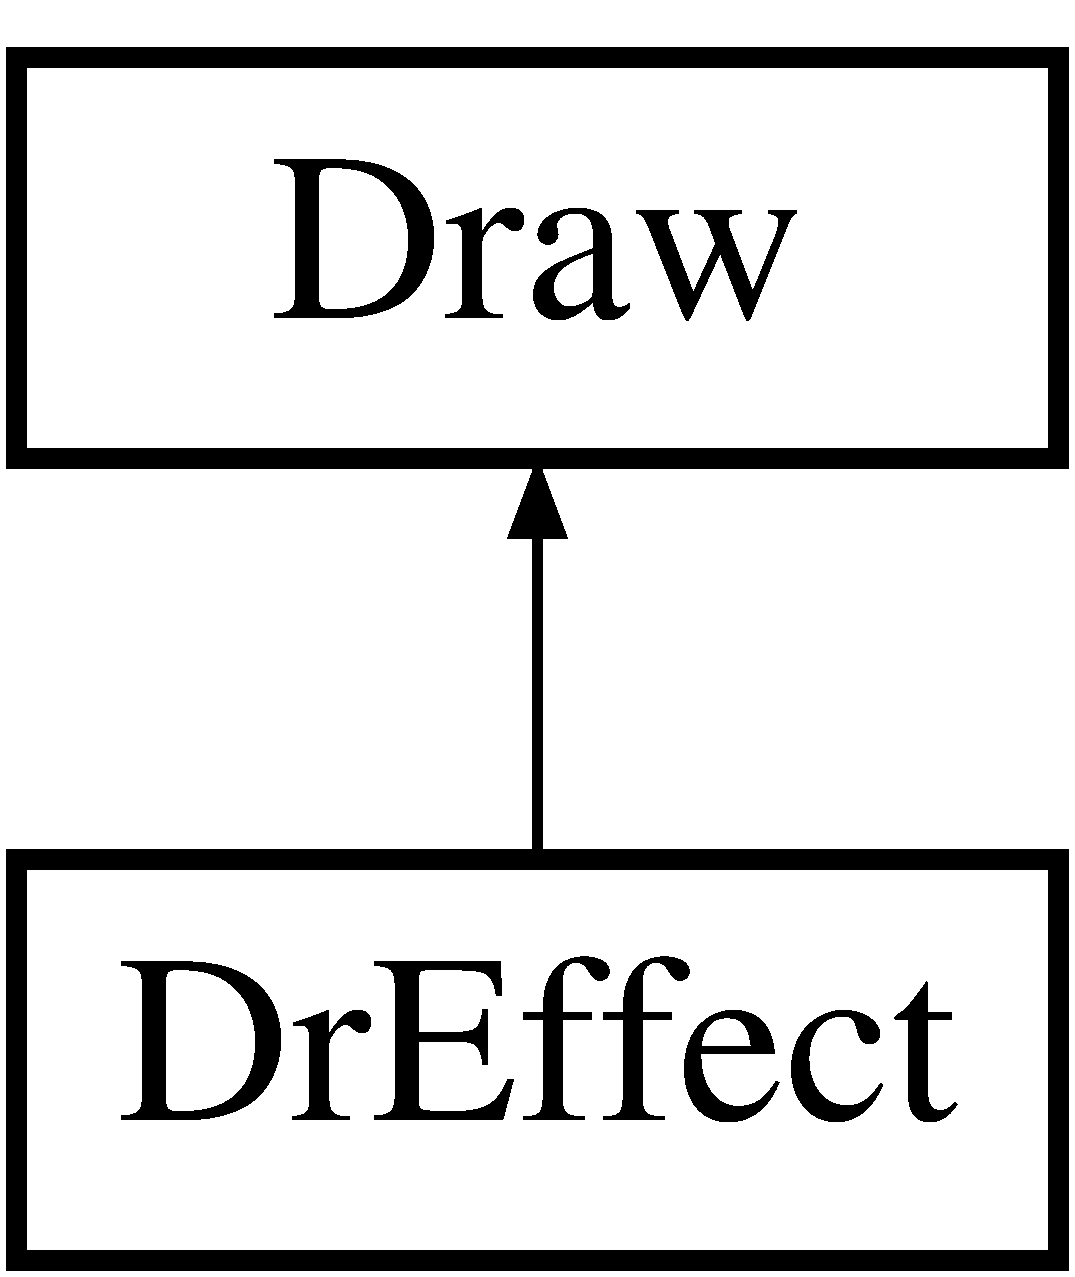
\includegraphics[height=2.000000cm]{classDrEffect}
\end{center}
\end{figure}
\subsubsection*{\-Public \-Member \-Functions}
\begin{DoxyCompactItemize}
\item 
\hypertarget{classDrEffect_a62e60652a984dcd65b592fde6e89ddbc}{void \hyperlink{classDrEffect_a62e60652a984dcd65b592fde6e89ddbc}{\-Effect\-Filter} ()}\label{classDrEffect_a62e60652a984dcd65b592fde6e89ddbc}

\begin{DoxyCompactList}\small\item\em \-Applies a filter to pixel. \end{DoxyCompactList}\item 
\hypertarget{classDrEffect_a3106c4097c47a929b15fb0bf788b161d}{void \hyperlink{classDrEffect_a3106c4097c47a929b15fb0bf788b161d}{\-Effect\-Motion} ()}\label{classDrEffect_a3106c4097c47a929b15fb0bf788b161d}

\begin{DoxyCompactList}\small\item\em \-Shifting of pixels. \end{DoxyCompactList}\item 
\hypertarget{classDrEffect_ae52c5b89d732c8cd4c027c2e6d82be39}{void \hyperlink{classDrEffect_ae52c5b89d732c8cd4c027c2e6d82be39}{\-Effect\-M\-C} ()}\label{classDrEffect_ae52c5b89d732c8cd4c027c2e6d82be39}

\begin{DoxyCompactList}\small\item\em \-Applies a random disposition of blocks. \end{DoxyCompactList}\item 
\hypertarget{classDrEffect_aab090cce7962df824dd04060dc002bc2}{void \hyperlink{classDrEffect_aab090cce7962df824dd04060dc002bc2}{\-Effect\-Coarse\-Grain} (int \-Grana)}\label{classDrEffect_aab090cce7962df824dd04060dc002bc2}

\begin{DoxyCompactList}\small\item\em \-Defocus the images in blocks. \end{DoxyCompactList}\item 
\hypertarget{classDrEffect_aadc5a450e9bf79186f43915f10886c0d}{void \hyperlink{classDrEffect_aadc5a450e9bf79186f43915f10886c0d}{\-Effect\-Increase} ()}\label{classDrEffect_aadc5a450e9bf79186f43915f10886c0d}

\begin{DoxyCompactList}\small\item\em \-Increase the resolution. \end{DoxyCompactList}\item 
\hypertarget{classDrEffect_aa3eca255b6be227d7d901cc2a72017a5}{void \hyperlink{classDrEffect_aa3eca255b6be227d7d901cc2a72017a5}{\-Run} ()}\label{classDrEffect_aa3eca255b6be227d7d901cc2a72017a5}

\begin{DoxyCompactList}\small\item\em \-Create an animation. \end{DoxyCompactList}\item 
void \hyperlink{classDrEffect_a98b1050f09da390896f964fb7a892391}{\-Initialize} ()
\item 
\hypertarget{classDrEffect_a8121ce6dcaabd895864fcb398d61830a}{void {\bfseries \-Histo} ()}\label{classDrEffect_a8121ce6dcaabd895864fcb398d61830a}

\item 
\hypertarget{classDrEffect_a4ac7178d0dc54a6e3ef5baf06f7c0f6a}{void {\bfseries \-Nabla\-Phi} ()}\label{classDrEffect_a4ac7178d0dc54a6e3ef5baf06f7c0f6a}

\item 
\hypertarget{classDrEffect_af982d1688f2311db74fc3f30bcdb793c}{void {\bfseries \-Black\-White} ()}\label{classDrEffect_af982d1688f2311db74fc3f30bcdb793c}

\item 
\hypertarget{classDrEffect_a79efe43daa44b6da6e1c3179c97625ed}{void {\bfseries \-D\-Reshape} (int weight, int height)}\label{classDrEffect_a79efe43daa44b6da6e1c3179c97625ed}

\item 
\hypertarget{classDrEffect_ac9184736d5fec94273a1784787a387c9}{void {\bfseries \-Dr\-Ekeyboard} (unsigned char key)}\label{classDrEffect_ac9184736d5fec94273a1784787a387c9}

\item 
\hypertarget{classDrEffect_a276658b556a1c7496e893a4888ffd0a0}{void {\bfseries \-Print\-Intensity} ()}\label{classDrEffect_a276658b556a1c7496e893a4888ffd0a0}

\item 
\hypertarget{classDrEffect_a87cab2148c827f9de25acf21b7b75e69}{int {\bfseries \-Contrast} ()}\label{classDrEffect_a87cab2148c827f9de25acf21b7b75e69}

\item 
\hypertarget{classDrEffect_ac569c02507323cdda29fb1e184932f26}{int {\bfseries \-Binary} (int \-Mode)}\label{classDrEffect_ac569c02507323cdda29fb1e184932f26}

\item 
\hypertarget{classDrEffect_aaf6edb6412f345f308004d4bbdfe6f21}{int {\bfseries \-Noise} (unsigned char $\ast$\hyperlink{classDraw_a45ed15a0527d5ba75107645dc8467078}{\-Picture}, unsigned char $\ast$\-Out\-Picture, int width, int height)}\label{classDrEffect_aaf6edb6412f345f308004d4bbdfe6f21}

\item 
\hypertarget{classDrEffect_aa3c03c8d0fad03bed05a7b4ed578c7f8}{int {\bfseries \-Swap\-Blocks} (unsigned char $\ast$\hyperlink{classDraw_a45ed15a0527d5ba75107645dc8467078}{\-Picture}, unsigned char $\ast$\-Out\-Picture, int width, int height, \hyperlink{structPERMUTE}{\-P\-E\-R\-M\-U\-T\-E} $\ast$\-Perm, int \-N\-Gridw, int \-N\-Gridh, int $\ast$\-Sequence1, int \-N\-Partition)}\label{classDrEffect_aa3c03c8d0fad03bed05a7b4ed578c7f8}

\item 
\hypertarget{classDrEffect_a8297413646e4367507222838aee867fd}{int {\bfseries \-Shift\-Blocks} (unsigned char $\ast$\hyperlink{classDraw_a45ed15a0527d5ba75107645dc8467078}{\-Picture}, unsigned char $\ast$\-Out\-Picture, int width, int height, int $\ast$\-Sequence, int \-N\-Gridw, int \-N\-Gridh, int $\ast$\-Sequence1, int \-N\-Partition)}\label{classDrEffect_a8297413646e4367507222838aee867fd}

\item 
\hypertarget{classDrEffect_a32440e0fb7b50f5934cda4d6b8af5cf6}{int {\bfseries \-Discretize} (unsigned char $\ast$\hyperlink{classDraw_a45ed15a0527d5ba75107645dc8467078}{\-Picture}, unsigned char $\ast$\-Out\-Picture, int \hyperlink{classDraw_ab92a87c2480115eaf15a27a8fa0cd965}{\-Im\-Width}, int \-Im\-Height, int \-W\-Width, int \-W\-Height, int \-Blockw, int \-Blokh)}\label{classDrEffect_a32440e0fb7b50f5934cda4d6b8af5cf6}

\item 
\hypertarget{classDrEffect_a8dfc2959f3fc3f77fa6fcba0d5a6ba0a}{int {\bfseries \-Edges} (unsigned char $\ast$\hyperlink{classDraw_a45ed15a0527d5ba75107645dc8467078}{\-Picture}, unsigned char $\ast$\-Out\-Picture, int width, int height)}\label{classDrEffect_a8dfc2959f3fc3f77fa6fcba0d5a6ba0a}

\item 
\hypertarget{classDrEffect_a5e807a9bb2fd73525054fdc5bbe2722d}{int {\bfseries \-Increase\-Resolution} (unsigned char $\ast$\hyperlink{classDraw_a45ed15a0527d5ba75107645dc8467078}{\-Picture}, unsigned char $\ast$\-Out\-Picture, int \hyperlink{classDraw_ab92a87c2480115eaf15a27a8fa0cd965}{\-Im\-Width}, int \-Im\-Height, int \-Times)}\label{classDrEffect_a5e807a9bb2fd73525054fdc5bbe2722d}

\item 
\hypertarget{classDrEffect_aebc416ae6d83d469837a19a3080555a1}{int {\bfseries \-Buff\-Size} ()}\label{classDrEffect_aebc416ae6d83d469837a19a3080555a1}

\end{DoxyCompactItemize}
\subsubsection*{\-Public \-Attributes}
\begin{DoxyCompactItemize}
\item 
\hypertarget{classDrEffect_ab838279ebd63d393a2b2d1869f938130}{int {\bfseries \-N\-Char}}\label{classDrEffect_ab838279ebd63d393a2b2d1869f938130}

\item 
\hypertarget{classDrEffect_aab4995eedc5bb0d45d86f0e2a5d0e869}{\hyperlink{classMatematica}{\-Matematica} $\ast$ {\bfseries \-Mat}}\label{classDrEffect_aab4995eedc5bb0d45d86f0e2a5d0e869}

\item 
\hypertarget{classDrEffect_a4c5ab80dcdf3fd65635f5aaf226b8134}{unsigned char {\bfseries \-Median} \mbox{[}4\mbox{]}}\label{classDrEffect_a4c5ab80dcdf3fd65635f5aaf226b8134}

\item 
\hypertarget{classDrEffect_a18ba95d201a709a76b4851c640d78cc3}{unsigned char {\bfseries \-Quart1} \mbox{[}4\mbox{]}}\label{classDrEffect_a18ba95d201a709a76b4851c640d78cc3}

\item 
\hypertarget{classDrEffect_a74095d8f0e65d6a5f72e6e9cb5b3a469}{unsigned char {\bfseries \-Quart3} \mbox{[}4\mbox{]}}\label{classDrEffect_a74095d8f0e65d6a5f72e6e9cb5b3a469}

\item 
\hypertarget{classDrEffect_a2d8866b988a2fa30ad757e8bfb06e572}{double $\ast$$\ast$ {\bfseries \-Hist}}\label{classDrEffect_a2d8866b988a2fa30ad757e8bfb06e572}

\item 
\hypertarget{classDrEffect_a7bc31eadf9a4b6f445e0108719dcebab}{double $\ast$$\ast$ {\bfseries \-Phi}}\label{classDrEffect_a7bc31eadf9a4b6f445e0108719dcebab}

\item 
\hypertarget{classDrEffect_a6ba57c41c047bfa956eff1c7086af325}{int $\ast$$\ast$ {\bfseries \-Patch}}\label{classDrEffect_a6ba57c41c047bfa956eff1c7086af325}

\end{DoxyCompactItemize}


\subsubsection{\-Detailed \-Description}


\-Definition at line 35 of file \-Dr\-Effect.\-h.



\subsubsection{\-Member \-Function \-Documentation}
\hypertarget{classDrEffect_a98b1050f09da390896f964fb7a892391}{\index{\-Dr\-Effect@{\-Dr\-Effect}!\-Initialize@{\-Initialize}}
\index{\-Initialize@{\-Initialize}!DrEffect@{\-Dr\-Effect}}
\paragraph[{\-Initialize}]{\setlength{\rightskip}{0pt plus 5cm}void {\bf \-Initialize} (
\begin{DoxyParamCaption}
{}
\end{DoxyParamCaption}
)}}\label{classDrEffect_a98b1050f09da390896f964fb7a892391}
\-The numbers refers to \-Stephens \-Mora \-Tka'cik \-Bialek \-Thermodynamics of natural images 

\-Definition at line 3 of file \-Dr\-Definition.\-cpp.



\-References \-Matematica\-::\-Transform().



\-The documentation for this class was generated from the following files\-:\begin{DoxyCompactItemize}
\item 
src/\-Dr\-Effect/\-Dr\-Effect.\-h\item 
src/\-Dr\-Effect/\-Dr\-Definition.\-cpp\item 
src/\-Dr\-Effect/\-Dr\-Open\-G\-L.\-cpp\end{DoxyCompactItemize}

\hypertarget{classDrFinestra}{}\subsection{Dr\+Finestra Class Reference}
\label{classDrFinestra}\index{Dr\+Finestra@{Dr\+Finestra}}
Inheritance diagram for Dr\+Finestra\+:\begin{figure}[H]
\begin{center}
\leavevmode
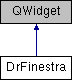
\includegraphics[height=2.000000cm]{classDrFinestra}
\end{center}
\end{figure}
\subsubsection*{Public Member Functions}
\begin{DoxyCompactItemize}
\item 
{\bfseries Dr\+Finestra} (Q\+Widget $\ast$parent=0, const char $\ast$name=0)\hypertarget{classDrFinestra_af085fd34d2ae2fbd63c5e0ed97e5bb81}{}\label{classDrFinestra_af085fd34d2ae2fbd63c5e0ed97e5bb81}

\item 
void {\bfseries Histo} ()\hypertarget{classDrFinestra_a8121ce6dcaabd895864fcb398d61830a}{}\label{classDrFinestra_a8121ce6dcaabd895864fcb398d61830a}

\item 
void {\bfseries Data\+File} (char $\ast$File\+Name)\hypertarget{classDrFinestra_aafb2f0d8d425b1ae361f7bf1dd4c587f}{}\label{classDrFinestra_aafb2f0d8d425b1ae361f7bf1dd4c587f}

\item 
void {\bfseries Conf\+File} (char $\ast$File\+Name)\hypertarget{classDrFinestra_a418fd69a796855fc20dcdaf6bb94fc68}{}\label{classDrFinestra_a418fd69a796855fc20dcdaf6bb94fc68}

\item 
void {\bfseries Run} ()\hypertarget{classDrFinestra_aa3eca255b6be227d7d901cc2a72017a5}{}\label{classDrFinestra_aa3eca255b6be227d7d901cc2a72017a5}

\end{DoxyCompactItemize}


\subsubsection{Detailed Description}


Definition at line 21 of file Dr\+Finestra.\+h.



The documentation for this class was generated from the following files\+:\begin{DoxyCompactItemize}
\item 
src/\+Dr\+Effect/Dr\+Finestra.\+h\item 
src/\+Dr\+Effect/Dr\+Finestra.\+cpp\end{DoxyCompactItemize}

\hypertarget{classDrScript}{\subsection{\-Dr\-Script \-Class \-Reference}
\label{classDrScript}\index{\-Dr\-Script@{\-Dr\-Script}}
}
\subsubsection*{\-Public \-Slots}
\begin{DoxyCompactItemize}
\item 
\hypertarget{classDrScript_a70532654904bf37033660923eec20d03}{void {\bfseries \-Incr\-Slide} ()}\label{classDrScript_a70532654904bf37033660923eec20d03}

\end{DoxyCompactItemize}
\subsubsection*{\-Public \-Member \-Functions}
\begin{DoxyCompactItemize}
\item 
\hypertarget{classDrScript_ad07dfe5f66c1f4e18d5f02ad418db10e}{void {\bfseries \-Exec\-Script} (\-Q\-Painter $\ast$p)}\label{classDrScript_ad07dfe5f66c1f4e18d5f02ad418db10e}

\item 
\hypertarget{classDrScript_a4e36cec6c1334987ee4466ad67b9a959}{void {\bfseries \-Read\-Slide} (\-Q\-Painter $\ast$p)}\label{classDrScript_a4e36cec6c1334987ee4466ad67b9a959}

\end{DoxyCompactItemize}
\subsubsection*{\-Protected \-Member \-Functions}
\begin{DoxyCompactItemize}
\item 
\hypertarget{classDrScript_ad06d035e601c42cc2a3b9d1229c73d36}{virtual void {\bfseries paint\-Event} (\-Q\-Paint\-Event $\ast$)}\label{classDrScript_ad06d035e601c42cc2a3b9d1229c73d36}

\end{DoxyCompactItemize}


\subsubsection{\-Detailed \-Description}


\-Definition at line 33 of file \-Dr\-Script.\-h.



\-The documentation for this class was generated from the following files\-:\begin{DoxyCompactItemize}
\item 
src/\-Dr\-Effect/\-Dr\-Script.\-h\item 
src/\-Dr\-Effect/\-Dr\-Script.\-cpp\end{DoxyCompactItemize}

\hypertarget{classElementiGrafici}{}\subsection{Elementi\+Grafici Class Reference}
\label{classElementiGrafici}\index{Elementi\+Grafici@{Elementi\+Grafici}}


Contains the function to interacts with the data stored in \hyperlink{classVarDatFile}{Var\+Dat\+File}.  




{\ttfamily \#include $<$Elementi\+Grafici.\+h$>$}

Inheritance diagram for Elementi\+Grafici\+:\begin{figure}[H]
\begin{center}
\leavevmode
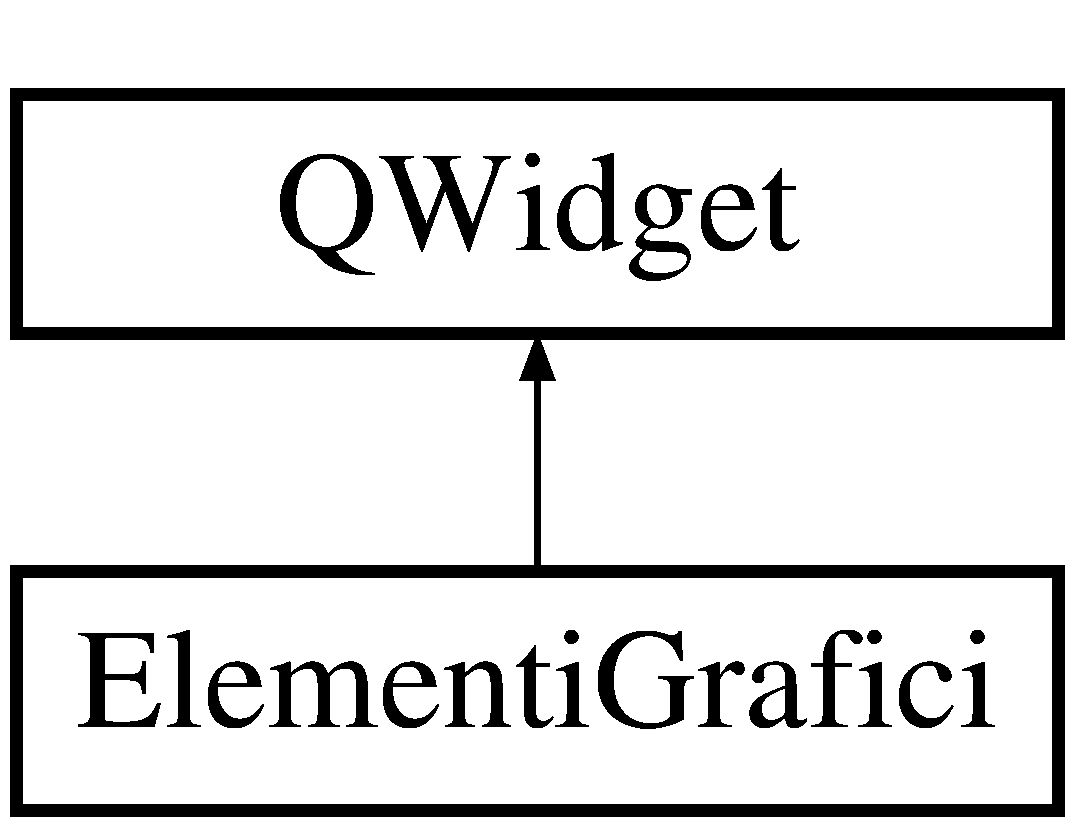
\includegraphics[height=2.000000cm]{classElementiGrafici}
\end{center}
\end{figure}
\subsubsection*{Public Slots}
\begin{DoxyCompactItemize}
\item 
void \hyperlink{classElementiGrafici_a3584d9fda1661c9d984821a0ff2da530}{Imp\+N\+Bin} (int n)\hypertarget{classElementiGrafici_a3584d9fda1661c9d984821a0ff2da530}{}\label{classElementiGrafici_a3584d9fda1661c9d984821a0ff2da530}

\begin{DoxyCompactList}\small\item\em Set N\+Bin. \end{DoxyCompactList}\item 
void \hyperlink{classElementiGrafici_acf8b3f1f0d2c774fac0dc94d45d08b14}{Imp\+N\+Mobile} (int n)\hypertarget{classElementiGrafici_acf8b3f1f0d2c774fac0dc94d45d08b14}{}\label{classElementiGrafici_acf8b3f1f0d2c774fac0dc94d45d08b14}

\begin{DoxyCompactList}\small\item\em Set the bins for the running average. \end{DoxyCompactList}\item 
void \hyperlink{classElementiGrafici_a1f447e7c93ae89ef6e13cca8f2076e94}{Imp\+N\+Correla} (int n)\hypertarget{classElementiGrafici_a1f447e7c93ae89ef6e13cca8f2076e94}{}\label{classElementiGrafici_a1f447e7c93ae89ef6e13cca8f2076e94}

\begin{DoxyCompactList}\small\item\em Set the bins for the point correlation. \end{DoxyCompactList}\item 
void \hyperlink{classElementiGrafici_a234790a4188b9c368be09d366b2b89cc}{Imp\+N\+Vis\+Min} (int n)\hypertarget{classElementiGrafici_a234790a4188b9c368be09d366b2b89cc}{}\label{classElementiGrafici_a234790a4188b9c368be09d366b2b89cc}

\begin{DoxyCompactList}\small\item\em Set the minimum visualisation point. \end{DoxyCompactList}\item 
void \hyperlink{classElementiGrafici_a11a67a0bdbf5cd5ce699585b39bc6bd5}{Imp\+N\+Vis\+Max} (int n)\hypertarget{classElementiGrafici_a11a67a0bdbf5cd5ce699585b39bc6bd5}{}\label{classElementiGrafici_a11a67a0bdbf5cd5ce699585b39bc6bd5}

\begin{DoxyCompactList}\small\item\em Set the maximum visualisation point. \end{DoxyCompactList}\item 
void \hyperlink{classElementiGrafici_ae2314ccdec0ece989ce7e791a7346efb}{Imp\+N\+El\+Min} (int n)\hypertarget{classElementiGrafici_ae2314ccdec0ece989ce7e791a7346efb}{}\label{classElementiGrafici_ae2314ccdec0ece989ce7e791a7346efb}

\begin{DoxyCompactList}\small\item\em Set the minimum elaboration point. \end{DoxyCompactList}\item 
void \hyperlink{classElementiGrafici_a2cd7d7fb138ce7fd90c1497d012c9e99}{Imp\+N\+El\+Max} (int n)\hypertarget{classElementiGrafici_a2cd7d7fb138ce7fd90c1497d012c9e99}{}\label{classElementiGrafici_a2cd7d7fb138ce7fd90c1497d012c9e99}

\begin{DoxyCompactList}\small\item\em Set the maximum elaboration point. \end{DoxyCompactList}\item 
void {\bfseries Imp\+N\+El\+MinY} (int n)\hypertarget{classElementiGrafici_aadcdbf87a4c1dca7df80a7c653a6a943}{}\label{classElementiGrafici_aadcdbf87a4c1dca7df80a7c653a6a943}

\item 
void {\bfseries Imp\+N\+El\+MaxY} (int n)\hypertarget{classElementiGrafici_a27bd0ef54a4c6b52b2f4c6d9601bd97a}{}\label{classElementiGrafici_a27bd0ef54a4c6b52b2f4c6d9601bd97a}

\item 
void {\bfseries Imp\+Inter} (int n)\hypertarget{classElementiGrafici_a9755534e507f3cd602bfdcfc75a14bba}{}\label{classElementiGrafici_a9755534e507f3cd602bfdcfc75a14bba}

\item 
void {\bfseries Imp\+Inter\+El} (int n)\hypertarget{classElementiGrafici_a7466d2c78345091214c066e06153da64}{}\label{classElementiGrafici_a7466d2c78345091214c066e06153da64}

\item 
void {\bfseries Imp\+CoordX} (int n)\hypertarget{classElementiGrafici_aa90f637b1171afa46cc439442a823dac}{}\label{classElementiGrafici_aa90f637b1171afa46cc439442a823dac}

\item 
void {\bfseries Imp\+CoordY} (int n)\hypertarget{classElementiGrafici_ab694182834d32f19148fce74e38bcda0}{}\label{classElementiGrafici_ab694182834d32f19148fce74e38bcda0}

\item 
void \hyperlink{classElementiGrafici_a24700e3e45a706f7cc9ecc6a86349aa2}{Imp\+Coord\+DY} (int n)\hypertarget{classElementiGrafici_a24700e3e45a706f7cc9ecc6a86349aa2}{}\label{classElementiGrafici_a24700e3e45a706f7cc9ecc6a86349aa2}

\begin{DoxyCompactList}\small\item\em Set the y error bar. \end{DoxyCompactList}\item 
void \hyperlink{classElementiGrafici_a392a5f9549a38ad82a7f6e4963550aed}{Imp\+N\+VarX} (int n, int m)
\begin{DoxyCompactList}\small\item\em Type for coordinate change. \end{DoxyCompactList}\item 
void {\bfseries Imp\+N\+VarY} (int n, int m)\hypertarget{classElementiGrafici_a29bb5fb3f1cae3a4c778ee4b94b56096}{}\label{classElementiGrafici_a29bb5fb3f1cae3a4c778ee4b94b56096}

\item 
void {\bfseries Imp\+Inter} (int n, int m)\hypertarget{classElementiGrafici_a81bb6df8a851297f9a49c8ba8b4c6a8c}{}\label{classElementiGrafici_a81bb6df8a851297f9a49c8ba8b4c6a8c}

\item 
void {\bfseries Imp\+Inter\+El} (int n, int m)\hypertarget{classElementiGrafici_ae58a48a8d5227bb75ceb9a3fdc46f3e5}{}\label{classElementiGrafici_ae58a48a8d5227bb75ceb9a3fdc46f3e5}

\item 
void {\bfseries Imp\+InterY} (int n, int m)\hypertarget{classElementiGrafici_a142174ea062ee7cd6c8a4567089b7302}{}\label{classElementiGrafici_a142174ea062ee7cd6c8a4567089b7302}

\item 
void {\bfseries Apri} ()\hypertarget{classElementiGrafici_a7ce426fbebfb112e79be160c5dabb7a8}{}\label{classElementiGrafici_a7ce426fbebfb112e79be160c5dabb7a8}

\item 
void {\bfseries Apri} (char $\ast$$\ast$argv, int $\ast$File\+List, int N\+File)\hypertarget{classElementiGrafici_a348285e35871cf0c33b78e99ada91daf}{}\label{classElementiGrafici_a348285e35871cf0c33b78e99ada91daf}

\item 
void {\bfseries Apri\+Ext} (double $\ast$$\ast$Ext\+St, int Ext\+N\+Max, int Ext\+N\+Var, int Ext\+N\+Bin)\hypertarget{classElementiGrafici_afd8f1c7dfdb7c0e0ce1e58abe4c10491}{}\label{classElementiGrafici_afd8f1c7dfdb7c0e0ce1e58abe4c10491}

\item 
void {\bfseries Apri\+Ext} (\hyperlink{classVarDatFile}{Var\+Dat\+File} $\ast$Extv1)\hypertarget{classElementiGrafici_a7e686314b411f0ea6c67d7ae048829ff}{}\label{classElementiGrafici_a7e686314b411f0ea6c67d7ae048829ff}

\item 
void {\bfseries Aggiungi} ()\hypertarget{classElementiGrafici_ae5ca66a932311e9241fd5a19bcb71df9}{}\label{classElementiGrafici_ae5ca66a932311e9241fd5a19bcb71df9}

\item 
void {\bfseries Punti\+Segnale} ()\hypertarget{classElementiGrafici_a19020236a1891d63ef61683900a14339}{}\label{classElementiGrafici_a19020236a1891d63ef61683900a14339}

\item 
void {\bfseries Punti\+Distribuzione} ()\hypertarget{classElementiGrafici_a8173ea1c5803ffb3d49d519c6ba6bd62}{}\label{classElementiGrafici_a8173ea1c5803ffb3d49d519c6ba6bd62}

\item 
void {\bfseries Punti\+Somma\+Segnali} ()\hypertarget{classElementiGrafici_a7d0091b09fc90defa5dc08753c6f7548}{}\label{classElementiGrafici_a7d0091b09fc90defa5dc08753c6f7548}

\item 
void {\bfseries Punti\+Inter\+Rett} ()\hypertarget{classElementiGrafici_a0bf5647190e07ca5bdc66479b68a83dc}{}\label{classElementiGrafici_a0bf5647190e07ca5bdc66479b68a83dc}

\item 
void {\bfseries Punti\+Inter\+Exp} ()\hypertarget{classElementiGrafici_a2c1948aa11cce55281310900e1605104}{}\label{classElementiGrafici_a2c1948aa11cce55281310900e1605104}

\item 
void {\bfseries Punti\+Inter\+Gauss} ()\hypertarget{classElementiGrafici_a43f8b0d90b1f2776248c7d5a09ce2f52}{}\label{classElementiGrafici_a43f8b0d90b1f2776248c7d5a09ce2f52}

\item 
void {\bfseries Punti\+Parabola} ()\hypertarget{classElementiGrafici_a1393b81f822fa22f65aedbe024e12a35}{}\label{classElementiGrafici_a1393b81f822fa22f65aedbe024e12a35}

\item 
void {\bfseries Punti\+Media\+Mob} ()\hypertarget{classElementiGrafici_a621d3caabee812742838dab1560911a7}{}\label{classElementiGrafici_a621d3caabee812742838dab1560911a7}

\item 
void {\bfseries Punti\+Correla\+A\+Due} ()\hypertarget{classElementiGrafici_a339f2e9121f34842a7a9d892473ca76d}{}\label{classElementiGrafici_a339f2e9121f34842a7a9d892473ca76d}

\item 
void {\bfseries Punti\+Autosimilarita} ()\hypertarget{classElementiGrafici_aeb7bdddb656328f04527f78a19e897c2}{}\label{classElementiGrafici_aeb7bdddb656328f04527f78a19e897c2}

\item 
void {\bfseries Punti\+Integrale} ()\hypertarget{classElementiGrafici_a0dbefe819b9529cb93f3983338767507}{}\label{classElementiGrafici_a0dbefe819b9529cb93f3983338767507}

\item 
void {\bfseries Punti\+Derivata} ()\hypertarget{classElementiGrafici_a5a07b596cf34e93ba01127121d90377a}{}\label{classElementiGrafici_a5a07b596cf34e93ba01127121d90377a}

\item 
void {\bfseries Punti\+Varie} ()\hypertarget{classElementiGrafici_a2cf0c4c0d8c7a6031f53692cc50e0fc6}{}\label{classElementiGrafici_a2cf0c4c0d8c7a6031f53692cc50e0fc6}

\item 
void {\bfseries Punti\+Spettro} ()\hypertarget{classElementiGrafici_a84933b6dd02965ac4c048ff7c63ccc9a}{}\label{classElementiGrafici_a84933b6dd02965ac4c048ff7c63ccc9a}

\item 
void {\bfseries Punti\+Normalizza} ()\hypertarget{classElementiGrafici_af4ee838cad0f2db9cedadc5bf17f3d70}{}\label{classElementiGrafici_af4ee838cad0f2db9cedadc5bf17f3d70}

\item 
void {\bfseries Punti\+Modulo} ()\hypertarget{classElementiGrafici_ab7917b17fcae1846f36cfd4615d88fdf}{}\label{classElementiGrafici_ab7917b17fcae1846f36cfd4615d88fdf}

\item 
void {\bfseries Punti\+Radice} ()\hypertarget{classElementiGrafici_ab4984079f4f62e6e7848ccbf9a6ee99f}{}\label{classElementiGrafici_ab4984079f4f62e6e7848ccbf9a6ee99f}

\item 
void {\bfseries Punti\+Autocor} ()\hypertarget{classElementiGrafici_a4047dbf5363ac26fec5f224921b474d6}{}\label{classElementiGrafici_a4047dbf5363ac26fec5f224921b474d6}

\item 
void {\bfseries Punti\+Sum} ()\hypertarget{classElementiGrafici_ad76417399a6e317acf2db4ad14377796}{}\label{classElementiGrafici_ad76417399a6e317acf2db4ad14377796}

\item 
void {\bfseries Disegna\+Linee} ()\hypertarget{classElementiGrafici_aaf4729e6eaa6920c691fbde7d0a74279}{}\label{classElementiGrafici_aaf4729e6eaa6920c691fbde7d0a74279}

\item 
void {\bfseries Disegna\+Punti} ()\hypertarget{classElementiGrafici_a88ba06b0806d1508d706a4720cf95576}{}\label{classElementiGrafici_a88ba06b0806d1508d706a4720cf95576}

\item 
void {\bfseries Disegna\+Griglia} ()\hypertarget{classElementiGrafici_a432112ec4a583449f221ffcca2881627}{}\label{classElementiGrafici_a432112ec4a583449f221ffcca2881627}

\item 
void {\bfseries Disegna\+Logx} ()\hypertarget{classElementiGrafici_a9e45f519a13281c3ff0d3df0e305428f}{}\label{classElementiGrafici_a9e45f519a13281c3ff0d3df0e305428f}

\item 
void {\bfseries Disegna\+Logy} ()\hypertarget{classElementiGrafici_a3f42d94c22f6258ef28279c384d6cadc}{}\label{classElementiGrafici_a3f42d94c22f6258ef28279c384d6cadc}

\item 
void {\bfseries Se\+Riscala} ()\hypertarget{classElementiGrafici_ad02893236e5b30858927f97156b79280}{}\label{classElementiGrafici_ad02893236e5b30858927f97156b79280}

\item 
void {\bfseries Se\+Riscala\+Tutto} ()\hypertarget{classElementiGrafici_a51720bc39995d8710fb9f24bf57dc922}{}\label{classElementiGrafici_a51720bc39995d8710fb9f24bf57dc922}

\item 
void {\bfseries N\+Set} ()\hypertarget{classElementiGrafici_a58725b35c5fb4d5833b4bee464ae2011}{}\label{classElementiGrafici_a58725b35c5fb4d5833b4bee464ae2011}

\item 
void {\bfseries Stampa\+File} ()\hypertarget{classElementiGrafici_a73e375f008c0d0ea1dafc4f215f217e0}{}\label{classElementiGrafici_a73e375f008c0d0ea1dafc4f215f217e0}

\item 
void {\bfseries Punta\+Ext} (double $\ast$$\ast$Ext\+St, int n\+Var)\hypertarget{classElementiGrafici_a6dfbf3d00f9a30e895519026e5a524fc}{}\label{classElementiGrafici_a6dfbf3d00f9a30e895519026e5a524fc}

\item 
void {\bfseries Sul\+Segnale} (bool)\hypertarget{classElementiGrafici_aab89c647fd8087701ae2bd5649ac0e71}{}\label{classElementiGrafici_aab89c647fd8087701ae2bd5649ac0e71}

\item 
void {\bfseries Sul\+Grafico} (bool)\hypertarget{classElementiGrafici_ad28434da4f00671fa2bb44b21d650793}{}\label{classElementiGrafici_ad28434da4f00671fa2bb44b21d650793}

\item 
void {\bfseries SuX} (bool)\hypertarget{classElementiGrafici_a576e02963c06c6bf4093be751a05864a}{}\label{classElementiGrafici_a576e02963c06c6bf4093be751a05864a}

\item 
void {\bfseries SuY} (bool)\hypertarget{classElementiGrafici_abb76b56883789f3b2996fca37d4e5627}{}\label{classElementiGrafici_abb76b56883789f3b2996fca37d4e5627}

\item 
void {\bfseries Su\+DX} (bool)\hypertarget{classElementiGrafici_a7d191cc9235876312b5ffa331687f618}{}\label{classElementiGrafici_a7d191cc9235876312b5ffa331687f618}

\item 
void {\bfseries Su\+DY} (bool)\hypertarget{classElementiGrafici_abfb6855da4602206465bcfa5f9d7edc6}{}\label{classElementiGrafici_abfb6855da4602206465bcfa5f9d7edc6}

\item 
void {\bfseries Ridisegna} ()\hypertarget{classElementiGrafici_a16a08184aeafd1fee3a1ff7cda78ae9f}{}\label{classElementiGrafici_a16a08184aeafd1fee3a1ff7cda78ae9f}

\item 
void {\bfseries Info\+Stato} (const char $\ast$)\hypertarget{classElementiGrafici_af18e5840aacd449087ad7fd565376671}{}\label{classElementiGrafici_af18e5840aacd449087ad7fd565376671}

\item 
void {\bfseries Info\+Sequenza} (const char $\ast$)\hypertarget{classElementiGrafici_a5af720ba9134d54bf30ccdcedc0fdaef}{}\label{classElementiGrafici_a5af720ba9134d54bf30ccdcedc0fdaef}

\item 
void {\bfseries Salva} ()\hypertarget{classElementiGrafici_acee559dcef17096e6c09aff88342fdfc}{}\label{classElementiGrafici_acee559dcef17096e6c09aff88342fdfc}

\item 
void {\bfseries Nome\+File} (const Q\+String \&)\hypertarget{classElementiGrafici_aed7f5207ef3aa32ebbdb28c9a1c1d82d}{}\label{classElementiGrafici_aed7f5207ef3aa32ebbdb28c9a1c1d82d}

\item 
void {\bfseries Nome\+Conf} (const Q\+String \&)\hypertarget{classElementiGrafici_a7487a623cfe92920f8376426d7292f7a}{}\label{classElementiGrafici_a7487a623cfe92920f8376426d7292f7a}

\item 
void {\bfseries Nome\+Entrata} (const Q\+String \&)\hypertarget{classElementiGrafici_ad20a48546555e4f78208cfedcb1005a8}{}\label{classElementiGrafici_ad20a48546555e4f78208cfedcb1005a8}

\item 
void {\bfseries Nome\+Salva} (const Q\+String \&)\hypertarget{classElementiGrafici_a46f536be9337941aae2a4521fca51a82}{}\label{classElementiGrafici_a46f536be9337941aae2a4521fca51a82}

\item 
void {\bfseries Nome\+Uscita} (const Q\+String \&)\hypertarget{classElementiGrafici_a995123a940f17bf70d9d7a111615a8fe}{}\label{classElementiGrafici_a995123a940f17bf70d9d7a111615a8fe}

\item 
void {\bfseries Nome\+Titolo} (const Q\+String \&)\hypertarget{classElementiGrafici_ab2e2f8361f9be40f9c722b835081e490}{}\label{classElementiGrafici_ab2e2f8361f9be40f9c722b835081e490}

\item 
void {\bfseries Nome\+EtichettaX} (const Q\+String \&)\hypertarget{classElementiGrafici_a034404ea7cfd06269eb6e61846e26928}{}\label{classElementiGrafici_a034404ea7cfd06269eb6e61846e26928}

\item 
void {\bfseries Nome\+EtichettaY} (const Q\+String \&)\hypertarget{classElementiGrafici_aa996204f760abdafebc9c7d72910569c}{}\label{classElementiGrafici_aa996204f760abdafebc9c7d72910569c}

\item 
void {\bfseries Nome\+Tit} (const Q\+String \&)\hypertarget{classElementiGrafici_a46eb253dadb0c4a06f2b5fdd2162a9d6}{}\label{classElementiGrafici_a46eb253dadb0c4a06f2b5fdd2162a9d6}

\item 
void {\bfseries Nome\+EtX} (const Q\+String \&)\hypertarget{classElementiGrafici_a6e1e8b2acabaeaede11ea5cbff99095a}{}\label{classElementiGrafici_a6e1e8b2acabaeaede11ea5cbff99095a}

\item 
void {\bfseries Nome\+EtY} (const Q\+String \&)\hypertarget{classElementiGrafici_ac20d92b7f3d05acf28ba033209d35084}{}\label{classElementiGrafici_ac20d92b7f3d05acf28ba033209d35084}

\end{DoxyCompactItemize}
\subsubsection*{Signals}
\begin{DoxyCompactItemize}
\item 
void {\bfseries N\+Bin\+Cambiati} (int)\hypertarget{classElementiGrafici_a048f05ac3050c10ad7d654a15b621b3b}{}\label{classElementiGrafici_a048f05ac3050c10ad7d654a15b621b3b}

\item 
void {\bfseries N\+Mobile\+Cambiato} (int)\hypertarget{classElementiGrafici_a44748d7b5265b956ef38447b21de14e7}{}\label{classElementiGrafici_a44748d7b5265b956ef38447b21de14e7}

\item 
void {\bfseries N\+Correla\+Cambiato} (int)\hypertarget{classElementiGrafici_ab4584f4b6aa2a92d8029857fb071251b}{}\label{classElementiGrafici_ab4584f4b6aa2a92d8029857fb071251b}

\item 
void {\bfseries N\+Vis\+Min\+Cambiato} (int)\hypertarget{classElementiGrafici_a5c5ce178489f03e118bf9266445b8f35}{}\label{classElementiGrafici_a5c5ce178489f03e118bf9266445b8f35}

\item 
void {\bfseries N\+Vis\+Max\+Cambiato} (int)\hypertarget{classElementiGrafici_a4f198fc5e2298c073b0ec579ce032993}{}\label{classElementiGrafici_a4f198fc5e2298c073b0ec579ce032993}

\item 
void {\bfseries N\+El\+Min\+Cambiato} (int)\hypertarget{classElementiGrafici_ab59cc52d78aca2c8fae65dbbe3f36f5a}{}\label{classElementiGrafici_ab59cc52d78aca2c8fae65dbbe3f36f5a}

\item 
void {\bfseries N\+El\+Max\+Cambiato} (int)\hypertarget{classElementiGrafici_a44518ba5db7b571e90c846fb586cbc6f}{}\label{classElementiGrafici_a44518ba5db7b571e90c846fb586cbc6f}

\item 
void {\bfseries N\+El\+Min\+Y\+Cambiato} (int)\hypertarget{classElementiGrafici_a27270206b03a27838d796040936b750e}{}\label{classElementiGrafici_a27270206b03a27838d796040936b750e}

\item 
void {\bfseries N\+El\+Max\+Y\+Cambiato} (int)\hypertarget{classElementiGrafici_aef66138bfb4f5efb3bf47dce79618125}{}\label{classElementiGrafici_aef66138bfb4f5efb3bf47dce79618125}

\item 
void {\bfseries Logx\+Cambiato} (bool)\hypertarget{classElementiGrafici_ad58d1afd3b004eb469b7abf4f742c1bd}{}\label{classElementiGrafici_ad58d1afd3b004eb469b7abf4f742c1bd}

\item 
void {\bfseries Logy\+Cambiato} (bool)\hypertarget{classElementiGrafici_af5df39800e88ee47c4f8c53de47361d8}{}\label{classElementiGrafici_af5df39800e88ee47c4f8c53de47361d8}

\item 
void {\bfseries Media\+Cambiata} (int)\hypertarget{classElementiGrafici_a5ff411f9adf0dbf16adb44b4833aab26}{}\label{classElementiGrafici_a5ff411f9adf0dbf16adb44b4833aab26}

\item 
void {\bfseries Scarto\+Cambiato} (int)\hypertarget{classElementiGrafici_a0bc4c2c0fd8938943d583dfa40f7ddee}{}\label{classElementiGrafici_a0bc4c2c0fd8938943d583dfa40f7ddee}

\item 
void {\bfseries Inter\+Vis\+Cambiato} (int)\hypertarget{classElementiGrafici_ab2b787678a3269ec3ecf38db21fd0599}{}\label{classElementiGrafici_ab2b787678a3269ec3ecf38db21fd0599}

\item 
void {\bfseries Inter\+El\+Cambiato} (int)\hypertarget{classElementiGrafici_a994799116f49708665255dfddaf9c386}{}\label{classElementiGrafici_a994799116f49708665255dfddaf9c386}

\item 
void {\bfseries Inter\+Vis\+Cambiato} (int, int)\hypertarget{classElementiGrafici_a21c34fe68599603a47f69601167b35a4}{}\label{classElementiGrafici_a21c34fe68599603a47f69601167b35a4}

\item 
void {\bfseries Inter\+El\+Cambiato} (int, int)\hypertarget{classElementiGrafici_a8e9c506fd492ca1fef062678291e20c9}{}\label{classElementiGrafici_a8e9c506fd492ca1fef062678291e20c9}

\item 
void {\bfseries Inter\+Y\+Cambiato} (int, int)\hypertarget{classElementiGrafici_a6796e23be4aa4645df4d135ad083d438}{}\label{classElementiGrafici_a6796e23be4aa4645df4d135ad083d438}

\item 
void {\bfseries Coord\+X\+Cambiata} (int)\hypertarget{classElementiGrafici_aaeb550b26be79d351aeac16c7e231c01}{}\label{classElementiGrafici_aaeb550b26be79d351aeac16c7e231c01}

\item 
void {\bfseries Coord\+Y\+Cambiata} (int)\hypertarget{classElementiGrafici_aa3f284d3f9c14f9355df1263455e67d0}{}\label{classElementiGrafici_aa3f284d3f9c14f9355df1263455e67d0}

\item 
void {\bfseries Inter\+Coord\+X\+Cambiato} (int, int)\hypertarget{classElementiGrafici_a9a03ae9843fd6c285a8bff30f9007967}{}\label{classElementiGrafici_a9a03ae9843fd6c285a8bff30f9007967}

\item 
void {\bfseries Inter\+Coord\+Y\+Cambiato} (int, int)\hypertarget{classElementiGrafici_a2ff20475a2c5c09b8c287cd7644bf616}{}\label{classElementiGrafici_a2ff20475a2c5c09b8c287cd7644bf616}

\item 
void {\bfseries Fine\+Simulazione} ()\hypertarget{classElementiGrafici_ac25a3538940ac2801f4ad56f88bb5431}{}\label{classElementiGrafici_ac25a3538940ac2801f4ad56f88bb5431}

\item 
void {\bfseries Segnale\+Grafico} (bool)\hypertarget{classElementiGrafici_ade0934ab4f0d2c6478a6ea78c67e226a}{}\label{classElementiGrafici_ade0934ab4f0d2c6478a6ea78c67e226a}

\item 
void {\bfseries Stato} (const Q\+String \&)\hypertarget{classElementiGrafici_a4f8f107f3febb4508e66460cc2a27869}{}\label{classElementiGrafici_a4f8f107f3febb4508e66460cc2a27869}

\item 
void {\bfseries Stato\+Sequenza} (const Q\+String \&)\hypertarget{classElementiGrafici_ae6439c322b85e158ef740d29da6996f4}{}\label{classElementiGrafici_ae6439c322b85e158ef740d29da6996f4}

\item 
void {\bfseries Testo\+Cambiato} (const Q\+String \&)\hypertarget{classElementiGrafici_a1923e73eff067c21de15f2c47337c908}{}\label{classElementiGrafici_a1923e73eff067c21de15f2c47337c908}

\item 
void {\bfseries Conf\+Cambiato} (const Q\+String \&)\hypertarget{classElementiGrafici_aba58ae180a94049c73531bbbf80a32a1}{}\label{classElementiGrafici_aba58ae180a94049c73531bbbf80a32a1}

\item 
void {\bfseries Salva\+Cambiato} (const Q\+String \&)\hypertarget{classElementiGrafici_a906601bbe3b6dd319b69368b37b3e720}{}\label{classElementiGrafici_a906601bbe3b6dd319b69368b37b3e720}

\item 
void {\bfseries Titolo\+Cambiato} (const Q\+String \&)\hypertarget{classElementiGrafici_a28ca485da9971393014fa46e848db22c}{}\label{classElementiGrafici_a28ca485da9971393014fa46e848db22c}

\item 
void {\bfseries Etichetta\+X\+Cambiato} (const Q\+String \&)\hypertarget{classElementiGrafici_aaaa30fb8074a7136b82e00ca70df78b5}{}\label{classElementiGrafici_aaaa30fb8074a7136b82e00ca70df78b5}

\item 
void {\bfseries Etichetta\+Y\+Cambiato} (const Q\+String \&)\hypertarget{classElementiGrafici_a8788351212b4df62d5fd4c13cc61d483}{}\label{classElementiGrafici_a8788351212b4df62d5fd4c13cc61d483}

\end{DoxyCompactItemize}
\subsubsection*{Public Member Functions}
\begin{DoxyCompactItemize}
\item 
\hyperlink{classElementiGrafici_aae49d2145b40fce2fbcee668b2934669}{Elementi\+Grafici} (Q\+Widget $\ast$parent=0, const char $\ast$name=0)\hypertarget{classElementiGrafici_aae49d2145b40fce2fbcee668b2934669}{}\label{classElementiGrafici_aae49d2145b40fce2fbcee668b2934669}

\begin{DoxyCompactList}\small\item\em General constructor. \end{DoxyCompactList}\item 
\hyperlink{classElementiGrafici_ae572bae1d4f4a3c6aa1d40edb62bdaf0}{$\sim$\+Elementi\+Grafici} ()\hypertarget{classElementiGrafici_ae572bae1d4f4a3c6aa1d40edb62bdaf0}{}\label{classElementiGrafici_ae572bae1d4f4a3c6aa1d40edb62bdaf0}

\begin{DoxyCompactList}\small\item\em Destructor. \end{DoxyCompactList}\item 
Q\+Size\+Policy {\bfseries Dimensionamento} () const \hypertarget{classElementiGrafici_ab6fbc22c59252cb6152e25ca454a6595}{}\label{classElementiGrafici_ab6fbc22c59252cb6152e25ca454a6595}

\item 
void \hyperlink{classElementiGrafici_a61a52933f2e84207a3ef7c376ce7df38}{Choose\+Data\+File} (char $\ast$File\+Name)\hypertarget{classElementiGrafici_a61a52933f2e84207a3ef7c376ce7df38}{}\label{classElementiGrafici_a61a52933f2e84207a3ef7c376ce7df38}

\begin{DoxyCompactList}\small\item\em Choose the input file. \end{DoxyCompactList}\item 
void \hyperlink{classElementiGrafici_a942934affd7a22cfa6d0297f89217292}{Choose\+Conf\+File} (char $\ast$File\+Name)\hypertarget{classElementiGrafici_a942934affd7a22cfa6d0297f89217292}{}\label{classElementiGrafici_a942934affd7a22cfa6d0297f89217292}

\begin{DoxyCompactList}\small\item\em Choose the configuration file. \end{DoxyCompactList}\end{DoxyCompactItemize}
\subsubsection*{Public Attributes}
\begin{DoxyCompactItemize}
\item 
int \hyperlink{classElementiGrafici_a35e5db5990993f09236122f4dfaf7bc3}{N\+Max}\hypertarget{classElementiGrafici_a35e5db5990993f09236122f4dfaf7bc3}{}\label{classElementiGrafici_a35e5db5990993f09236122f4dfaf7bc3}

\begin{DoxyCompactList}\small\item\em Number of points per array. \end{DoxyCompactList}\item 
int \hyperlink{classElementiGrafici_a4e1e3a7469a7fc5af310a17c2c2c787a}{N\+Dis}\hypertarget{classElementiGrafici_a4e1e3a7469a7fc5af310a17c2c2c787a}{}\label{classElementiGrafici_a4e1e3a7469a7fc5af310a17c2c2c787a}

\begin{DoxyCompactList}\small\item\em Current number of visualisation (debugging) \end{DoxyCompactList}\item 
\hyperlink{classVarDatFile}{Var\+Dat\+File} $\ast$ \hyperlink{classElementiGrafici_af8d0da3e35bb5e28aba9329efffbfb95}{v1}\hypertarget{classElementiGrafici_af8d0da3e35bb5e28aba9329efffbfb95}{}\label{classElementiGrafici_af8d0da3e35bb5e28aba9329efffbfb95}

\begin{DoxyCompactList}\small\item\em Class for the file handle. \end{DoxyCompactList}\item 
char $\ast$ \hyperlink{classElementiGrafici_ae062c77de5b1cd6767e9b53846eb76fe}{nome\+File}\hypertarget{classElementiGrafici_ae062c77de5b1cd6767e9b53846eb76fe}{}\label{classElementiGrafici_ae062c77de5b1cd6767e9b53846eb76fe}

\begin{DoxyCompactList}\small\item\em Name of the current file opened. \end{DoxyCompactList}\item 
char $\ast$ \hyperlink{classElementiGrafici_a8bf6d3f7358b88169b52d2b2f03a94f6}{nome\+Conf}\hypertarget{classElementiGrafici_a8bf6d3f7358b88169b52d2b2f03a94f6}{}\label{classElementiGrafici_a8bf6d3f7358b88169b52d2b2f03a94f6}

\begin{DoxyCompactList}\small\item\em Name of the config file. \end{DoxyCompactList}\item 
char $\ast$ \hyperlink{classElementiGrafici_a516c32509a9d2ba2c9f7e53fcdbd9ce0}{nome\+Salva}\hypertarget{classElementiGrafici_a516c32509a9d2ba2c9f7e53fcdbd9ce0}{}\label{classElementiGrafici_a516c32509a9d2ba2c9f7e53fcdbd9ce0}

\begin{DoxyCompactList}\small\item\em Name of the output file. \end{DoxyCompactList}\item 
Q\+String \hyperlink{classElementiGrafici_a99be08b66bcb34c0eaed5636e717154e}{nome\+Tit}\hypertarget{classElementiGrafici_a99be08b66bcb34c0eaed5636e717154e}{}\label{classElementiGrafici_a99be08b66bcb34c0eaed5636e717154e}

\begin{DoxyCompactList}\small\item\em Title name. \end{DoxyCompactList}\item 
Q\+String \hyperlink{classElementiGrafici_a2237fc9b6764dc053b817d31bc133b3e}{nome\+EtX}\hypertarget{classElementiGrafici_a2237fc9b6764dc053b817d31bc133b3e}{}\label{classElementiGrafici_a2237fc9b6764dc053b817d31bc133b3e}

\begin{DoxyCompactList}\small\item\em X axis label. \end{DoxyCompactList}\item 
Q\+String \hyperlink{classElementiGrafici_a42f259c584d0d2e7aeb9967d149bd15e}{nome\+EtY}\hypertarget{classElementiGrafici_a42f259c584d0d2e7aeb9967d149bd15e}{}\label{classElementiGrafici_a42f259c584d0d2e7aeb9967d149bd15e}

\begin{DoxyCompactList}\small\item\em Y axis label. \end{DoxyCompactList}\end{DoxyCompactItemize}
\subsubsection*{Protected Member Functions}
\begin{DoxyCompactItemize}
\item 
virtual void {\bfseries paint\+Event} (Q\+Paint\+Event $\ast$)\hypertarget{classElementiGrafici_ad06d035e601c42cc2a3b9d1229c73d36}{}\label{classElementiGrafici_ad06d035e601c42cc2a3b9d1229c73d36}

\item 
virtual void {\bfseries mouse\+Move\+Event} (Q\+Mouse\+Event $\ast$)\hypertarget{classElementiGrafici_a88e672693c2cfdbaf9af942a58a8e1dd}{}\label{classElementiGrafici_a88e672693c2cfdbaf9af942a58a8e1dd}

\end{DoxyCompactItemize}


\subsubsection{Detailed Description}
Contains the function to interacts with the data stored in \hyperlink{classVarDatFile}{Var\+Dat\+File}. 

Definition at line 83 of file Elementi\+Grafici.\+h.



\subsubsection{Member Function Documentation}
\index{Elementi\+Grafici@{Elementi\+Grafici}!Imp\+N\+VarX@{Imp\+N\+VarX}}
\index{Imp\+N\+VarX@{Imp\+N\+VarX}!Elementi\+Grafici@{Elementi\+Grafici}}
\paragraph[{\texorpdfstring{Imp\+N\+VarX}{ImpNVarX}}]{\setlength{\rightskip}{0pt plus 5cm}void Imp\+N\+VarX (
\begin{DoxyParamCaption}
\item[{int}]{n, }
\item[{int}]{m}
\end{DoxyParamCaption}
)\hspace{0.3cm}{\ttfamily [slot]}}\hypertarget{classElementiGrafici_a392a5f9549a38ad82a7f6e4963550aed}{}\label{classElementiGrafici_a392a5f9549a38ad82a7f6e4963550aed}


Type for coordinate change. 

Pointer to a coordinate change function 

Definition at line 362 of file Elementi\+Grafici\+Comm.\+cpp.



Referenced by Choose\+Conf\+File().



The documentation for this class was generated from the following files\+:\begin{DoxyCompactItemize}
\item 
src/\+Avvis/Elementi\+Grafici.\+h\item 
src/\+Avvis/Elementi\+Grafici.\+cpp\item 
src/\+Avvis/Elementi\+Grafici\+Comm.\+cpp\item 
src/\+Avvis/Elementi\+Grafici\+Dis.\+cpp\item 
src/\+Avvis/Elementi\+Grafici\+El.\+cpp\item 
src/\+Avvis/moc\+\_\+\+Elementi\+Grafici.\+cpp\end{DoxyCompactItemize}

\hypertarget{classElPoly}{}\subsection{El\+Poly Class Reference}
\label{classElPoly}\index{El\+Poly@{El\+Poly}}


Operates and visualizes the information in the \hyperlink{classVarData}{Var\+Data} class.  




{\ttfamily \#include $<$El\+Poly.\+h$>$}

Inheritance diagram for El\+Poly\+:\begin{figure}[H]
\begin{center}
\leavevmode
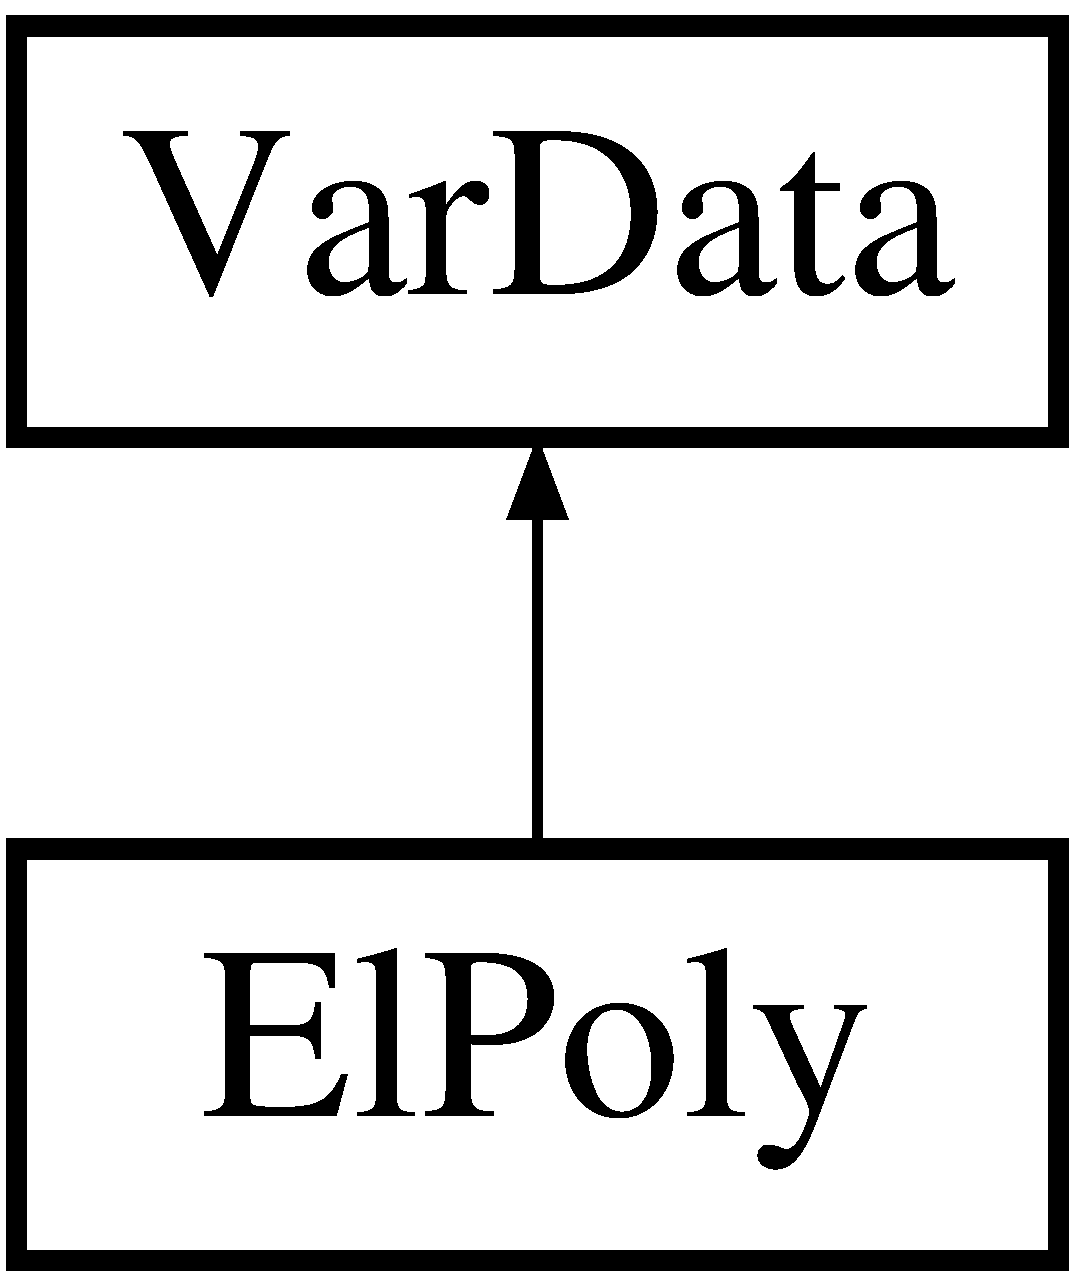
\includegraphics[height=2.000000cm]{classElPoly}
\end{center}
\end{figure}
\subsubsection*{Public Types}
\begin{DoxyCompactItemize}
\item 
typedef void(El\+Poly\+::$\ast$ \hyperlink{classElPoly_a7585cd93a8e979d9e6ee801bf63f3faa}{D\+R\+A\+W\+\_\+\+P\+A\+RT}) (int p)\hypertarget{classElPoly_a7585cd93a8e979d9e6ee801bf63f3faa}{}\label{classElPoly_a7585cd93a8e979d9e6ee801bf63f3faa}

\begin{DoxyCompactList}\small\item\em Data type for distance/field functions. \end{DoxyCompactList}\item 
typedef void(El\+Poly\+::$\ast$ \hyperlink{classElPoly_a38f050e6c22f58efb8582b7874f11193}{D\+R\+A\+W\+\_\+\+B\+O\+ND}) (double $\ast$Pos1, double $\ast$Pos2, float $\ast$Color)\hypertarget{classElPoly_a38f050e6c22f58efb8582b7874f11193}{}\label{classElPoly_a38f050e6c22f58efb8582b7874f11193}

\begin{DoxyCompactList}\small\item\em Data type for distance/field functions. \end{DoxyCompactList}\end{DoxyCompactItemize}
\subsubsection*{Public Member Functions}
\begin{DoxyCompactItemize}
\item 
\hyperlink{classElPoly_a98503475eca11a72b69cb62879d41183}{El\+Poly} (int argc, char $\ast$$\ast$argv, int $\ast$File\+Pos)\hypertarget{classElPoly_a98503475eca11a72b69cb62879d41183}{}\label{classElPoly_a98503475eca11a72b69cb62879d41183}

\begin{DoxyCompactList}\small\item\em Constructor. \end{DoxyCompactList}\item 
\hyperlink{classElPoly_afdf47e94336886931e93e716f32bb1ee}{$\sim$\+El\+Poly} ()\hypertarget{classElPoly_afdf47e94336886931e93e716f32bb1ee}{}\label{classElPoly_afdf47e94336886931e93e716f32bb1ee}

\begin{DoxyCompactList}\small\item\em Desctructor. \end{DoxyCompactList}\item 
int \hyperlink{classElPoly_a70302b7bbfa248d2963323bc63a4a292}{Dens\+Prof} (int N\+Bin, int N\+Sample, int Coord)
\begin{DoxyCompactList}\small\item\em Calculate the density profile  dens. \end{DoxyCompactList}\item 
void \hyperlink{classElPoly_aff1645802bd67fc1b5bfb3bb1884933a}{Dens\+Prof\+Normal\+Slab} (int N\+Bin, int N\+Sample, int Coord)
\begin{DoxyCompactList}\small\item\em Calculate the density profile projecting the particles on the normal density. \end{DoxyCompactList}\item 
int \hyperlink{classElPoly_a1c3688dd2704504d159802de5815643d}{Diff2\+Files} (int N\+Bin, int How)\hypertarget{classElPoly_a1c3688dd2704504d159802de5815643d}{}\label{classElPoly_a1c3688dd2704504d159802de5815643d}

\begin{DoxyCompactList}\small\item\em Density and thickness profile arond the nanoparticle. \end{DoxyCompactList}\item 
void \hyperlink{classElPoly_a019d255b1ff857ccd34550c7409a595b}{Rest\+Press} (int N\+Bin)\hypertarget{classElPoly_a019d255b1ff857ccd34550c7409a595b}{}\label{classElPoly_a019d255b1ff857ccd34550c7409a595b}

\begin{DoxyCompactList}\small\item\em Pressure difference between the virial and the ideal gas term. \end{DoxyCompactList}\item 
void \hyperlink{classElPoly_a3db31f8490f0ea101281679a270e72fe}{Slab\+Prof} (int N\+Bin, int n\+Nano, int Coord1)
\begin{DoxyCompactList}\small\item\em Thickness and density profile along Coord1. \end{DoxyCompactList}\item 
void \hyperlink{classElPoly_a6591e29bd7876dc9dc255808d04499f9}{Print\+Dens} (F\+I\+LE $\ast$File\+To\+Write, double $\ast$$\ast$Plot, double $\ast$Lat\+Dim, int N\+Bin)
\begin{DoxyCompactList}\small\item\em Print the density profile in the surfaces representation. \end{DoxyCompactList}\item 
void \hyperlink{classElPoly_a7c40fb501bdadab09ee7cf8d99259299}{Rad\+Dens2\+Thick} (int N\+Bin)
\begin{DoxyCompactList}\small\item\em Calculate the thickness from the radial density profile. \end{DoxyCompactList}\item 
void \hyperlink{classElPoly_ad5ab39cdaa856caea3463819b436e7b9}{Rad\+Dens2\+Thick2d} (int N\+Bin)
\begin{DoxyCompactList}\small\item\em Calculate the thickness from the radial density profile. \end{DoxyCompactList}\item 
int \hyperlink{classElPoly_ad0651bcc7574507f16c1998b57822bdd}{Temperature} (int N\+Bin, int Coord)\hypertarget{classElPoly_ad0651bcc7574507f16c1998b57822bdd}{}\label{classElPoly_ad0651bcc7574507f16c1998b57822bdd}

\begin{DoxyCompactList}\small\item\em Spatial distribution of the temperature. \end{DoxyCompactList}\item 
void \hyperlink{classElPoly_ac946a8b29f4eec0816699ce0c0cac23c}{Cart\+Dens} (int N\+Bin, int n\+Nano)
\begin{DoxyCompactList}\small\item\em 3d (rad,norma,dens) density profile in cartesian coordinates \end{DoxyCompactList}\item 
void \hyperlink{classElPoly_aff852b942203d47f2e21e2616537cbdd}{Rad\+DistrF} (int N\+Bin, int How, int n\+Nano)
\begin{DoxyCompactList}\small\item\em 3d (rad,norma,dens) density profile with respect to a initial position  rad\+Nano rad\+Cm rad\+CmN \end{DoxyCompactList}\item 
void \hyperlink{classElPoly_a932a57ab32bd20f60bce8b498ca3095d}{Bond\+Distr} (int N\+Sample)
\begin{DoxyCompactList}\small\item\em Distribution of the bond lengths. \end{DoxyCompactList}\item 
void \hyperlink{classElPoly_adac974d49c2d38f45c0227afe7c8fec9}{E2\+E\+Distr} (int N\+Sample)\hypertarget{classElPoly_adac974d49c2d38f45c0227afe7c8fec9}{}\label{classElPoly_adac974d49c2d38f45c0227afe7c8fec9}

\begin{DoxyCompactList}\small\item\em Distribution of end to end distances. \end{DoxyCompactList}\item 
void \hyperlink{classElPoly_aab448d2a574f63977ddcacb58db616e1}{Splay\+Distr} (int N\+Sample)
\begin{DoxyCompactList}\small\item\em Distribution of end to end distances. \end{DoxyCompactList}\item 
int \hyperlink{classElPoly_a64e019ffaa4437477ea433f7b5113341}{Radial\+Shell} (int N\+Bin)\hypertarget{classElPoly_a64e019ffaa4437477ea433f7b5113341}{}\label{classElPoly_a64e019ffaa4437477ea433f7b5113341}

\begin{DoxyCompactList}\small\item\em Outer shell of a projected (rad,normal) graph. \end{DoxyCompactList}\item 
int \hyperlink{classElPoly_af9a89c5f8dc4c7274ec5e00ff4db78bb}{Nano\+Particle} (int N\+Bin)\hypertarget{classElPoly_af9a89c5f8dc4c7274ec5e00ff4db78bb}{}\label{classElPoly_af9a89c5f8dc4c7274ec5e00ff4db78bb}

\begin{DoxyCompactList}\small\item\em Diffusion and density profile around the nanoparticle  nano. \end{DoxyCompactList}\item 
int \hyperlink{classElPoly_ad6fa03abf69921d9a0759689569e35e9}{WormF} (int Partition, int N\+Bin)\hypertarget{classElPoly_ad6fa03abf69921d9a0759689569e35e9}{}\label{classElPoly_ad6fa03abf69921d9a0759689569e35e9}

\begin{DoxyCompactList}\small\item\em Density profile of a non straight worm shape membrane  worm. \end{DoxyCompactList}\item 
void \hyperlink{classElPoly_aba321cce3649252deca41a462b0e3d38}{StalkF} (int N\+Sample)\hypertarget{classElPoly_aba321cce3649252deca41a462b0e3d38}{}\label{classElPoly_aba321cce3649252deca41a462b0e3d38}

\begin{DoxyCompactList}\small\item\em Separate the leaflets. \end{DoxyCompactList}\item 
void \hyperlink{classElPoly_abcf175509352ac9dd90cb8ad96494219}{Thick\+From\+Dens} (int N\+Bin)
\begin{DoxyCompactList}\small\item\em Calculate the thickness profile from the density plot. \end{DoxyCompactList}\item 
void \hyperlink{classElPoly_a16d58960eae98f1ad67971068f12a22c}{Area\+DistrF} (int N\+Bin)\hypertarget{classElPoly_a16d58960eae98f1ad67971068f12a22c}{}\label{classElPoly_a16d58960eae98f1ad67971068f12a22c}

\begin{DoxyCompactList}\small\item\em Distribution of the areas around the protein. \end{DoxyCompactList}\item 
void \hyperlink{classElPoly_ad3a244bc00c2c8216b1f5cbd36699cdc}{Rad\+Norm\+Pos} (int N\+Bin, int N\+Grid)\hypertarget{classElPoly_ad3a244bc00c2c8216b1f5cbd36699cdc}{}\label{classElPoly_ad3a244bc00c2c8216b1f5cbd36699cdc}

\begin{DoxyCompactList}\small\item\em Radial profile of the normal position of the particles. \end{DoxyCompactList}\item 
int \hyperlink{classElPoly_af9a44196e456df096e96d914e19d85c9}{Surf\+Tens} (int N\+Bin)\hypertarget{classElPoly_af9a44196e456df096e96d914e19d85c9}{}\label{classElPoly_af9a44196e456df096e96d914e19d85c9}

\begin{DoxyCompactList}\small\item\em Radial summation of the 3d tension profile. \end{DoxyCompactList}\item 
void \hyperlink{classElPoly_a35c812e3cfa8e0031dc2b521e075c1c9}{Sum\+Tens} ()\hypertarget{classElPoly_a35c812e3cfa8e0031dc2b521e075c1c9}{}\label{classElPoly_a35c812e3cfa8e0031dc2b521e075c1c9}

\begin{DoxyCompactList}\small\item\em Sum more tension profile files. \end{DoxyCompactList}\item 
int \hyperlink{classElPoly_a534f27d79203f0b018acaedf41bbdb13}{Press\+Trace} ()\hypertarget{classElPoly_a534f27d79203f0b018acaedf41bbdb13}{}\label{classElPoly_a534f27d79203f0b018acaedf41bbdb13}

\begin{DoxyCompactList}\small\item\em Trace of the pressure profile. \end{DoxyCompactList}\item 
int \hyperlink{classElPoly_a17a99c936b16e1880291e6c3c5957e44}{Press\+Radial} ()\hypertarget{classElPoly_a17a99c936b16e1880291e6c3c5957e44}{}\label{classElPoly_a17a99c936b16e1880291e6c3c5957e44}

\begin{DoxyCompactList}\small\item\em Contour plot around the inclusion. \end{DoxyCompactList}\item 
int \hyperlink{classElPoly_a7282d2e3fe0a3ee0caa631363913cc0a}{Tens2d\+Cart\+Rad} ()\hypertarget{classElPoly_a7282d2e3fe0a3ee0caa631363913cc0a}{}\label{classElPoly_a7282d2e3fe0a3ee0caa631363913cc0a}

\begin{DoxyCompactList}\small\item\em Change the pressure profile from cartesian to radial. \end{DoxyCompactList}\item 
void \hyperlink{classElPoly_adbfe7fc41363f770eee9c2a9e0e1ed57}{Stalk\+Line\+ProfF} (int N\+Bin)
\begin{DoxyCompactList}\small\item\em Write the line describing a linear stalk. \end{DoxyCompactList}\item 
void \hyperlink{classElPoly_a47cedfc639fa29b9812167b4fb5d1360}{Prova} ()\hypertarget{classElPoly_a47cedfc639fa29b9812167b4fb5d1360}{}\label{classElPoly_a47cedfc639fa29b9812167b4fb5d1360}

\begin{DoxyCompactList}\small\item\em Dummy function to operate on a sequence of files. \end{DoxyCompactList}\item 
void \hyperlink{classElPoly_a56b4b9780b4f84eb1713ca48b49fbbb2}{Pair\+Corr} (int N\+Bin, int N\+Dim)\hypertarget{classElPoly_a56b4b9780b4f84eb1713ca48b49fbbb2}{}\label{classElPoly_a56b4b9780b4f84eb1713ca48b49fbbb2}

\begin{DoxyCompactList}\small\item\em 1d pair correlation \end{DoxyCompactList}\item 
int \hyperlink{classElPoly_a7a3305d9ff38757faf367ced9abf89f0}{Pair\+CorrelationF} (int N\+Bin, int How)\hypertarget{classElPoly_a7a3305d9ff38757faf367ced9abf89f0}{}\label{classElPoly_a7a3305d9ff38757faf367ced9abf89f0}

\begin{DoxyCompactList}\small\item\em 1d, 2d pair correlation of the chains  pair\+Round pair\+Square (obsolete) \end{DoxyCompactList}\item 
int \hyperlink{classElPoly_a2f4aa8dc1e4dce0dc8fcb1d4b161757b}{Diffusivity} ()\hypertarget{classElPoly_a2f4aa8dc1e4dce0dc8fcb1d4b161757b}{}\label{classElPoly_a2f4aa8dc1e4dce0dc8fcb1d4b161757b}

\begin{DoxyCompactList}\small\item\em Diffusivity coefficient of the chains  diff. \end{DoxyCompactList}\item 
void \hyperlink{classElPoly_abf879a7d0b86a5eed8a5be87dc741200}{Diff\+Slab} (int N\+Slab)\hypertarget{classElPoly_abf879a7d0b86a5eed8a5be87dc741200}{}\label{classElPoly_abf879a7d0b86a5eed8a5be87dc741200}

\begin{DoxyCompactList}\small\item\em Diffusivity of particles starting from an initial slab. \end{DoxyCompactList}\item 
int \hyperlink{classElPoly_a1aa4889418bf8c589875e1c77b5262d2}{ScatteringF} (int N\+Bin, int How)\hypertarget{classElPoly_a1aa4889418bf8c589875e1c77b5262d2}{}\label{classElPoly_a1aa4889418bf8c589875e1c77b5262d2}

\begin{DoxyCompactList}\small\item\em 2d Scattering  scatt scatt2 \end{DoxyCompactList}\item 
int \hyperlink{classElPoly_afe2c794cc4f62f2e547526f63e82acfe}{N\+Chain\+P\+SquareF} ()\hypertarget{classElPoly_afe2c794cc4f62f2e547526f63e82acfe}{}\label{classElPoly_afe2c794cc4f62f2e547526f63e82acfe}

\begin{DoxyCompactList}\small\item\em Calculates the number of chain per area  area. \end{DoxyCompactList}\item 
void \hyperlink{classElPoly_afbe805e551084aebeee2c673c9b3937a}{Area\+Compr} (int N\+Sample)
\begin{DoxyCompactList}\small\item\em Calculates the number of chain per area  area. \end{DoxyCompactList}\item 
int \hyperlink{classElPoly_ada953db0b772595339ef925b5dbd8c62}{SpectrumF} (int N\+Bin)\hypertarget{classElPoly_ada953db0b772595339ef925b5dbd8c62}{}\label{classElPoly_ada953db0b772595339ef925b5dbd8c62}

\begin{DoxyCompactList}\small\item\em Calculates the 1d, 2d spectrum  spe. \end{DoxyCompactList}\item 
void \hyperlink{classElPoly_a16156b6e530ecc6df93b6ffd3c229f1b}{Midplane} (int N\+Bin)\hypertarget{classElPoly_a16156b6e530ecc6df93b6ffd3c229f1b}{}\label{classElPoly_a16156b6e530ecc6df93b6ffd3c229f1b}

\begin{DoxyCompactList}\small\item\em Midplanes for a sequence of snapshots. \end{DoxyCompactList}\item 
void \hyperlink{classElPoly_a669491e5e5c66f665694c9d8908d3109}{Spectrum\+Midplane} (int N\+Bin)\hypertarget{classElPoly_a669491e5e5c66f665694c9d8908d3109}{}\label{classElPoly_a669491e5e5c66f665694c9d8908d3109}

\begin{DoxyCompactList}\small\item\em Calculates the 1d, 2d spectrum  spe. \end{DoxyCompactList}\item 
void \hyperlink{classElPoly_a2eab2da94941b822d51d4e21bfe64aef}{Header\+Average} (int n\+Nano)\hypertarget{classElPoly_a2eab2da94941b822d51d4e21bfe64aef}{}\label{classElPoly_a2eab2da94941b822d51d4e21bfe64aef}

\begin{DoxyCompactList}\small\item\em Read the header and average the information. \end{DoxyCompactList}\item 
void \hyperlink{classElPoly_aa7a92147aff6a466398908e0f92ca139}{Widom\+Out} (char $\ast$In\+File, int N\+Bin)\hypertarget{classElPoly_aa7a92147aff6a466398908e0f92ca139}{}\label{classElPoly_aa7a92147aff6a466398908e0f92ca139}

\begin{DoxyCompactList}\small\item\em Create a system file with a chain less and the information about the missing chain. \end{DoxyCompactList}\item 
void \hyperlink{classElPoly_ab6f6a1fc647dcd4684fcaa667d612099}{Widom\+Out} ()\hypertarget{classElPoly_ab6f6a1fc647dcd4684fcaa667d612099}{}\label{classElPoly_ab6f6a1fc647dcd4684fcaa667d612099}

\begin{DoxyCompactList}\small\item\em Create N\+Ch systems with a chain less. \end{DoxyCompactList}\item 
void \hyperlink{classElPoly_a3e5c7ada1f6d5a2d37b23a9fb12771f9}{Widom\+In} (char $\ast$In\+File, int N\+Bin)\hypertarget{classElPoly_a3e5c7ada1f6d5a2d37b23a9fb12771f9}{}\label{classElPoly_a3e5c7ada1f6d5a2d37b23a9fb12771f9}

\begin{DoxyCompactList}\small\item\em Create the histogram of the energy of adding lipids. \end{DoxyCompactList}\item 
void \hyperlink{classElPoly_a2fbe8fbc91f83f0ac7a947965a3c38b8}{Widom\+In} ()\hypertarget{classElPoly_a2fbe8fbc91f83f0ac7a947965a3c38b8}{}\label{classElPoly_a2fbe8fbc91f83f0ac7a947965a3c38b8}

\begin{DoxyCompactList}\small\item\em Create a set of files with a chain more. \end{DoxyCompactList}\item 
void \hyperlink{classElPoly_a15ee2b235143aabc133fe974aa3258a2}{End2\+End\+Distr} (char $\ast$Out\+File)\hypertarget{classElPoly_a15ee2b235143aabc133fe974aa3258a2}{}\label{classElPoly_a15ee2b235143aabc133fe974aa3258a2}

\begin{DoxyCompactList}\small\item\em Write the end to end distance of the chains. \end{DoxyCompactList}\item 
void \hyperlink{classElPoly_af5a6c502bd65553e3f5e98577081ec66}{Bond\+Distr} (char $\ast$Out\+File, int N\+Bin)\hypertarget{classElPoly_af5a6c502bd65553e3f5e98577081ec66}{}\label{classElPoly_af5a6c502bd65553e3f5e98577081ec66}

\begin{DoxyCompactList}\small\item\em Write the bond distance between the monomers. \end{DoxyCompactList}\item 
void \hyperlink{classElPoly_a44e20767e332d941b94906f1a8e60e24}{Decoupling} (int What)\hypertarget{classElPoly_a44e20767e332d941b94906f1a8e60e24}{}\label{classElPoly_a44e20767e332d941b94906f1a8e60e24}

\begin{DoxyCompactList}\small\item\em Decoupling of the direction/end to end distance of the chains. \end{DoxyCompactList}\item 
void \hyperlink{classElPoly_a48968ddc44376e55852e9720b3827ebe}{Elastic\+Coupling} (int N\+Sample)
\begin{DoxyCompactList}\small\item\em Measure the elastic coupling between the two sheets. \end{DoxyCompactList}\item 
void \hyperlink{classElPoly_ab88192e9e4e0f11b68ad828d73ff8957}{Elastic\+Coupling\+N\+VT} ()
\begin{DoxyCompactList}\small\item\em Measure the elastic coupling between the two sheets. \end{DoxyCompactList}\item 
void \hyperlink{classElPoly_a6f1477b110e5ee0e7e027466dac51b69}{Bilayer\+Distance} (char $\ast$Out\+File, int N\+Bin)\hypertarget{classElPoly_a6f1477b110e5ee0e7e027466dac51b69}{}\label{classElPoly_a6f1477b110e5ee0e7e027466dac51b69}

\begin{DoxyCompactList}\small\item\em Measure the elastic coupling between the two sheets. \end{DoxyCompactList}\item 
void \hyperlink{classElPoly_a9152ea7044fdfac4a1def898c1c21a9d}{End\+To\+End\+Dist} ()\hypertarget{classElPoly_a9152ea7044fdfac4a1def898c1c21a9d}{}\label{classElPoly_a9152ea7044fdfac4a1def898c1c21a9d}

\begin{DoxyCompactList}\small\item\em Distribution of the end to end distances. \end{DoxyCompactList}\item 
int \hyperlink{classElPoly_aa2dbcd635807df0929968ec8932631ab}{ProjectionF} (int N\+Bin, int Coord)\hypertarget{classElPoly_aa2dbcd635807df0929968ec8932631ab}{}\label{classElPoly_aa2dbcd635807df0929968ec8932631ab}

\begin{DoxyCompactList}\small\item\em Projection of the system against one direction  pro. \end{DoxyCompactList}\item 
int \hyperlink{classElPoly_a04dd79cb2f5e46ae301b6dc1d57db28a}{CoreF} (int N\+Bin, int How)
\begin{DoxyCompactList}\small\item\em Sampling of the three dimentional space. \end{DoxyCompactList}\item 
int \hyperlink{classElPoly_a52844d3cee2d60eb47889fb021e10fc8}{Surface} (int N\+Bin, int Coord)\hypertarget{classElPoly_a52844d3cee2d60eb47889fb021e10fc8}{}\label{classElPoly_a52844d3cee2d60eb47889fb021e10fc8}

\begin{DoxyCompactList}\small\item\em Area of a surfuce projected on the coordinate Coord  surf. \end{DoxyCompactList}\item 
int \hyperlink{classElPoly_a4e71c4abd7c3ed37f29a8fcae064fd32}{From3\+To2d} (int Coord, double Param)\hypertarget{classElPoly_a4e71c4abd7c3ed37f29a8fcae064fd32}{}\label{classElPoly_a4e71c4abd7c3ed37f29a8fcae064fd32}

\begin{DoxyCompactList}\small\item\em Project the velocities of a 3d system on a 2d system wrt a coordinate. \end{DoxyCompactList}\item 
int \hyperlink{classElPoly_a30e6658740047a2fdd996e2b843e91b9}{From2\+To1d} (int Coord)\hypertarget{classElPoly_a30e6658740047a2fdd996e2b843e91b9}{}\label{classElPoly_a30e6658740047a2fdd996e2b843e91b9}

\begin{DoxyCompactList}\small\item\em Projet a 2d system on one of the two coordinates. \end{DoxyCompactList}\item 
int \hyperlink{classElPoly_a0b9109dcecbeec17c94472b5e638580a}{From3\+To1d} (int Coord)\hypertarget{classElPoly_a0b9109dcecbeec17c94472b5e638580a}{}\label{classElPoly_a0b9109dcecbeec17c94472b5e638580a}

\begin{DoxyCompactList}\small\item\em Project a 3d system on one coordinate. \end{DoxyCompactList}\item 
void \hyperlink{classElPoly_a23b08e53b2acd3090051d2034632c20f}{Iso\+Surf} (int N\+Sample, double $\ast$Iso\+Value, int N\+Iso)\hypertarget{classElPoly_a23b08e53b2acd3090051d2034632c20f}{}\label{classElPoly_a23b08e53b2acd3090051d2034632c20f}

\begin{DoxyCompactList}\small\item\em Density plot all over different snapshots and calculation of the isolevel surface. \end{DoxyCompactList}\item 
void \hyperlink{classElPoly_a7af346569b401863e3d5f4541e85e0c4}{Iso\+Line} (int N\+Sample, double $\ast$Iso\+Value, int N\+Iso, int How)\hypertarget{classElPoly_a7af346569b401863e3d5f4541e85e0c4}{}\label{classElPoly_a7af346569b401863e3d5f4541e85e0c4}

\begin{DoxyCompactList}\small\item\em Calculate the discrete density of the system and the correspondent isolines. \end{DoxyCompactList}\item 
void \hyperlink{classElPoly_a87faf7a81fea58a62dd97ee88b5b1b84}{Iso\+Line} (F\+I\+LE $\ast$F2\+Write, double $\ast$Plot, int N\+Sample, double $\ast$Iso\+Level, int N\+Iso)\hypertarget{classElPoly_a87faf7a81fea58a62dd97ee88b5b1b84}{}\label{classElPoly_a87faf7a81fea58a62dd97ee88b5b1b84}

\begin{DoxyCompactList}\small\item\em Perform the marching cubes on a density plot and print the isolines. \end{DoxyCompactList}\item 
void \hyperlink{classElPoly_a21a28de0471580af1978c3a48ae0ba0e}{Fetch\+Stalk} ()
\begin{DoxyCompactList}\small\item\em Write the position of the stalk for every snapshot. \end{DoxyCompactList}\item 
void \hyperlink{classElPoly_aecd33584d71ae498798338253cbf83f0}{Fetch\+Pore} ()\hypertarget{classElPoly_aecd33584d71ae498798338253cbf83f0}{}\label{classElPoly_aecd33584d71ae498798338253cbf83f0}

\begin{DoxyCompactList}\small\item\em Write the position of the pore for every snapshot. \end{DoxyCompactList}\item 
void \hyperlink{classElPoly_a099625012512857cb5524bf15b397e5e}{Stalk\+Area} ()
\begin{DoxyCompactList}\small\item\em Area of hydrophobic in the torus. \end{DoxyCompactList}\item 
void \hyperlink{classElPoly_aafe33ef0f28995ba7c1a778196decf9b}{Av\+Snap} ()\hypertarget{classElPoly_aafe33ef0f28995ba7c1a778196decf9b}{}\label{classElPoly_aafe33ef0f28995ba7c1a778196decf9b}

\begin{DoxyCompactList}\small\item\em Average the postion of the lipids over many snapshots. \end{DoxyCompactList}\item 
void \hyperlink{classElPoly_a4192d526e79a4c1e0b4910a4f35720c4}{Slab\+Angle\+Profs} (int N\+Bin, int N\+Angle, int Coord)
\begin{DoxyCompactList}\small\item\em Radial profiles of the slab density between 0⁰ and 90⁰ subdivided in N\+Angle angles. \end{DoxyCompactList}\item 
void \hyperlink{classElPoly_ada9b9ef0fea961264425fae43e3a4391}{Sample} (int N\+Sample)\hypertarget{classElPoly_ada9b9ef0fea961264425fae43e3a4391}{}\label{classElPoly_ada9b9ef0fea961264425fae43e3a4391}

\begin{DoxyCompactList}\small\item\em Sample the space in N\+Sample lattice points. \end{DoxyCompactList}\item 
void \hyperlink{classElPoly_ab03f8f580a4b45968aedcaa0d088c469}{Conv2\+Tecplot} (int N\+Bin, int How)\hypertarget{classElPoly_ab03f8f580a4b45968aedcaa0d088c469}{}\label{classElPoly_ab03f8f580a4b45968aedcaa0d088c469}

\begin{DoxyCompactList}\small\item\em Prepare a countor plot for tecplot. \end{DoxyCompactList}\item 
void \hyperlink{classElPoly_a552193e7b9dea6d667fc1cd2ecab1482}{Conv2\+Vmd} ()\hypertarget{classElPoly_a552193e7b9dea6d667fc1cd2ecab1482}{}\label{classElPoly_a552193e7b9dea6d667fc1cd2ecab1482}

\begin{DoxyCompactList}\small\item\em esport the data in vmd file format \end{DoxyCompactList}\item 
void \hyperlink{classElPoly_ac2e836951a966bd69b21705cad363b95}{Conv2\+Povray} ()\hypertarget{classElPoly_ac2e836951a966bd69b21705cad363b95}{}\label{classElPoly_ac2e836951a966bd69b21705cad363b95}

\begin{DoxyCompactList}\small\item\em esport the data in pov file format for rendering \end{DoxyCompactList}\item 
void \hyperlink{classElPoly_a538747fd3f643c9d171a00a5ec371ccc}{Conv2rzd} (int N\+Sample)\hypertarget{classElPoly_a538747fd3f643c9d171a00a5ec371ccc}{}\label{classElPoly_a538747fd3f643c9d171a00a5ec371ccc}

\begin{DoxyCompactList}\small\item\em esport the data in radius depth density file format \end{DoxyCompactList}\item 
void \hyperlink{classElPoly_ad9aa947dfbb4fd8d4f2eb314efc17730}{Conv2xyzd} (int N\+Sample)\hypertarget{classElPoly_ad9aa947dfbb4fd8d4f2eb314efc17730}{}\label{classElPoly_ad9aa947dfbb4fd8d4f2eb314efc17730}

\begin{DoxyCompactList}\small\item\em esport the data in radius depth density file format \end{DoxyCompactList}\item 
void \hyperlink{classElPoly_aee301bfab80a5bff74d1929e63cdbf0f}{Dr\+Field} (int N\+Grid, double Iso\+Level, int n\+Nano, F\+I\+LE $\ast$F\+Write)\hypertarget{classElPoly_aee301bfab80a5bff74d1929e63cdbf0f}{}\label{classElPoly_aee301bfab80a5bff74d1929e63cdbf0f}

\begin{DoxyCompactList}\small\item\em \hyperlink{classDraw}{Draw} a scalar field. \end{DoxyCompactList}\item 
void \hyperlink{classElPoly_a1d6d8bfcdb851627bb183cb803353270}{Dr\+Bond\+Pov\+Ray} (double $\ast$Pos1, double $\ast$Pos2, float $\ast$Color)\hypertarget{classElPoly_a1d6d8bfcdb851627bb183cb803353270}{}\label{classElPoly_a1d6d8bfcdb851627bb183cb803353270}

\begin{DoxyCompactList}\small\item\em \hyperlink{classDraw}{Draw} the bonds. \end{DoxyCompactList}\item 
void \hyperlink{classElPoly_a79715be09324f2b58cc98385a5f62e7b}{Header\+Pov\+Ray} ()\hypertarget{classElPoly_a79715be09324f2b58cc98385a5f62e7b}{}\label{classElPoly_a79715be09324f2b58cc98385a5f62e7b}

\begin{DoxyCompactList}\small\item\em Print the header for povray. \end{DoxyCompactList}\item 
void \hyperlink{classElPoly_a760f4fa1edbecc53d532140617dbf8ab}{Dr\+Nano\+Pov\+Ray} (int n)\hypertarget{classElPoly_a760f4fa1edbecc53d532140617dbf8ab}{}\label{classElPoly_a760f4fa1edbecc53d532140617dbf8ab}

\begin{DoxyCompactList}\small\item\em Pov\+Ray draw function. \end{DoxyCompactList}\item 
void \hyperlink{classElPoly_aedbaa04884ac62d32f3cce78fdfd92b8}{Dr\+Part\+Pov\+Ray} (int p)\hypertarget{classElPoly_aedbaa04884ac62d32f3cce78fdfd92b8}{}\label{classElPoly_aedbaa04884ac62d32f3cce78fdfd92b8}

\begin{DoxyCompactList}\small\item\em Pov\+Ray draw function. \end{DoxyCompactList}\item 
void \hyperlink{classElPoly_a3e03070150b93328661ff2c857eebbf4}{Conv\+Lattice} (int N\+Sample, char $\ast$F\+Name)\hypertarget{classElPoly_a3e03070150b93328661ff2c857eebbf4}{}\label{classElPoly_a3e03070150b93328661ff2c857eebbf4}

\begin{DoxyCompactList}\small\item\em Convert into a square lattice. \end{DoxyCompactList}\item 
void \hyperlink{classElPoly_abfd537703af91a0dceb86c6bba5bd213}{Remove\+Chains} ()\hypertarget{classElPoly_abfd537703af91a0dceb86c6bba5bd213}{}\label{classElPoly_abfd537703af91a0dceb86c6bba5bd213}

\begin{DoxyCompactList}\small\item\em Remove chains satisfying a condition. \end{DoxyCompactList}\item 
int \hyperlink{classElPoly_ae3aab8086f988eecdd12b8f29f45a56a}{Angle} (int N\+Bin)\hypertarget{classElPoly_ae3aab8086f988eecdd12b8f29f45a56a}{}\label{classElPoly_ae3aab8086f988eecdd12b8f29f45a56a}

\begin{DoxyCompactList}\small\item\em Calculation of the contact angle  angle Boh? \end{DoxyCompactList}\item 
double \hyperlink{classElPoly_a2dd3ba2334c4444c4ef406347618c170}{Contact\+Angle} (double x)\hypertarget{classElPoly_a2dd3ba2334c4444c4ef406347618c170}{}\label{classElPoly_a2dd3ba2334c4444c4ef406347618c170}

\begin{DoxyCompactList}\small\item\em Definition of the contact angle function Boh. \end{DoxyCompactList}\item 
int \hyperlink{classElPoly_a59529de9a660df4734a218130963ae25}{Center\+Of\+Mass} (int Coord)\hypertarget{classElPoly_a59529de9a660df4734a218130963ae25}{}\label{classElPoly_a59529de9a660df4734a218130963ae25}

\begin{DoxyCompactList}\small\item\em Averaged center of mass Boh. \end{DoxyCompactList}\item 
int \hyperlink{classElPoly_a5fa485410c0b7e02f523f96f33504435}{Change\+File} ()\hypertarget{classElPoly_a5fa485410c0b7e02f523f96f33504435}{}\label{classElPoly_a5fa485410c0b7e02f523f96f33504435}

\begin{DoxyCompactList}\small\item\em Defines the first and the last file to be elaborated  file. \end{DoxyCompactList}\item 
int \hyperlink{classElPoly_af3b99b4a504ae35256dfa33c9f1bfd31}{Specify\+Coord} ()\hypertarget{classElPoly_af3b99b4a504ae35256dfa33c9f1bfd31}{}\label{classElPoly_af3b99b4a504ae35256dfa33c9f1bfd31}

\begin{DoxyCompactList}\small\item\em Defines the normal coordinate  coord. \end{DoxyCompactList}\item 
int \hyperlink{classElPoly_a3432306726a27b310ec27b3900894b11}{Open\+File} (int f)\hypertarget{classElPoly_a3432306726a27b310ec27b3900894b11}{}\label{classElPoly_a3432306726a27b310ec27b3900894b11}

\begin{DoxyCompactList}\small\item\em Opens the f file of the list  open. \end{DoxyCompactList}\item 
int \hyperlink{classElPoly_a5ddc1cdb4d65932381030dba86448813}{Open\+File} (char $\ast$File\+Name)\hypertarget{classElPoly_a5ddc1cdb4d65932381030dba86448813}{}\label{classElPoly_a5ddc1cdb4d65932381030dba86448813}

\begin{DoxyCompactList}\small\item\em Opens a file. \end{DoxyCompactList}\item 
int \hyperlink{classElPoly_ae41ade7fbfd977babf42a7e2e6b33f07}{PropertiesF} ()\hypertarget{classElPoly_ae41ade7fbfd977babf42a7e2e6b33f07}{}\label{classElPoly_ae41ade7fbfd977babf42a7e2e6b33f07}

\begin{DoxyCompactList}\small\item\em Calculates some properties of the system  prop. \end{DoxyCompactList}\item 
char $\ast$ \hyperlink{classElPoly_a86e52eb42d4ead5eb6b800ab1fd3a4d2}{Choose\+Draw} (int Ext\+What2\+Draw)\hypertarget{classElPoly_a86e52eb42d4ead5eb6b800ab1fd3a4d2}{}\label{classElPoly_a86e52eb42d4ead5eb6b800ab1fd3a4d2}

\begin{DoxyCompactList}\small\item\em Convert the internal definition for the menu of \hyperlink{classElPoly}{El\+Poly} in string. \end{DoxyCompactList}\item 
void \hyperlink{classElPoly_aba70049e8fa7f7b845f9ccd8ad700015}{Choose\+Draw} (char $\ast$String)
\begin{DoxyCompactList}\small\item\em Assing the correct value of What2\+Draw from. \end{DoxyCompactList}\item 
void \hyperlink{classElPoly_acffadf1cdc641927dfd8af49eebc2069}{Divide\+Layers} (int How)\hypertarget{classElPoly_acffadf1cdc641927dfd8af49eebc2069}{}\label{classElPoly_acffadf1cdc641927dfd8af49eebc2069}

\begin{DoxyCompactList}\small\item\em Reorder the L\+I\+P\+ID block in four different layers. \end{DoxyCompactList}\item 
void \hyperlink{classElPoly_a464eca35e2fcc5f03f9f8be8702f36cc}{Set\+Bound\+File} (int Init\+File, int End\+File)\hypertarget{classElPoly_a464eca35e2fcc5f03f9f8be8702f36cc}{}\label{classElPoly_a464eca35e2fcc5f03f9f8be8702f36cc}

\begin{DoxyCompactList}\small\item\em Set the initial and final number of files. \end{DoxyCompactList}\item 
void \hyperlink{classElPoly_a02045f98c00a6ef6af607bc27fc3e82a}{Processing} (int f)\hypertarget{classElPoly_a02045f98c00a6ef6af607bc27fc3e82a}{}\label{classElPoly_a02045f98c00a6ef6af607bc27fc3e82a}

\begin{DoxyCompactList}\small\item\em Information on the current file elaborated. \end{DoxyCompactList}\item 
void \hyperlink{classElPoly_a2d5b51a7f120a4104f6e5070ca6c55f5}{Shift2\+Center} ()\hypertarget{classElPoly_a2d5b51a7f120a4104f6e5070ca6c55f5}{}\label{classElPoly_a2d5b51a7f120a4104f6e5070ca6c55f5}

\begin{DoxyCompactList}\small\item\em Shift the system to the center. \end{DoxyCompactList}\item 
void \hyperlink{classElPoly_adf3c4c944496227c17ceebc8d42d5ea5}{Set\+Back\+Fold} (int Bf)\hypertarget{classElPoly_adf3c4c944496227c17ceebc8d42d5ea5}{}\label{classElPoly_adf3c4c944496227c17ceebc8d42d5ea5}

\begin{DoxyCompactList}\small\item\em Set backfold type. \end{DoxyCompactList}\item 
void \hyperlink{classElPoly_a0312cac4bd3e684fef174d0147607a1c}{Set\+N\+Vis\+Skip} (int N\+Skip)\hypertarget{classElPoly_a0312cac4bd3e684fef174d0147607a1c}{}\label{classElPoly_a0312cac4bd3e684fef174d0147607a1c}

\begin{DoxyCompactList}\small\item\em Set backfold type. \end{DoxyCompactList}\item 
void \hyperlink{classElPoly_a6387005443a530d1a66a0833c72b23fd}{Render\+Part} (void)\hypertarget{classElPoly_a6387005443a530d1a66a0833c72b23fd}{}\label{classElPoly_a6387005443a530d1a66a0833c72b23fd}

\begin{DoxyCompactList}\small\item\em Choose the visualisation (obsolete) \end{DoxyCompactList}\item 
void \hyperlink{classElPoly_a28d17ecbad071d90ae8b571f068d865a}{Dr\+Run\+Time} ()\hypertarget{classElPoly_a28d17ecbad071d90ae8b571f068d865a}{}\label{classElPoly_a28d17ecbad071d90ae8b571f068d865a}

\begin{DoxyCompactList}\small\item\em Draws in run time (expensive) \end{DoxyCompactList}\item 
void \hyperlink{classElPoly_aef35a22a4138fad89d7329d9fd49d97e}{Dr\+Color} ()\hypertarget{classElPoly_aef35a22a4138fad89d7329d9fd49d97e}{}\label{classElPoly_aef35a22a4138fad89d7329d9fd49d97e}

\begin{DoxyCompactList}\small\item\em Visualisation of the particle system with velocity color scheme. \end{DoxyCompactList}\item 
void \hyperlink{classElPoly_ae89cedb0e996d10ec5f96e14f1f867cf}{Dr\+Part\+List} ()\hypertarget{classElPoly_ae89cedb0e996d10ec5f96e14f1f867cf}{}\label{classElPoly_ae89cedb0e996d10ec5f96e14f1f867cf}

\begin{DoxyCompactList}\small\item\em Create a list of all the particles. \end{DoxyCompactList}\item 
void \hyperlink{classElPoly_a3eef417e007c18f604455cfb38a948cb}{Dr\+Vector} (\hyperlink{classVettore}{Vettore} v, \hyperlink{classVettore}{Vettore} Origin)\hypertarget{classElPoly_a3eef417e007c18f604455cfb38a948cb}{}\label{classElPoly_a3eef417e007c18f604455cfb38a948cb}

\begin{DoxyCompactList}\small\item\em \hyperlink{classDraw}{Draw} a vector. \end{DoxyCompactList}\item 
void \hyperlink{classElPoly_a9968be2f08ada4e898c92c7e8552ac63}{Dr\+Vectors} ()\hypertarget{classElPoly_a9968be2f08ada4e898c92c7e8552ac63}{}\label{classElPoly_a9968be2f08ada4e898c92c7e8552ac63}

\begin{DoxyCompactList}\small\item\em \hyperlink{classDraw}{Draw} the chains as vectors. \end{DoxyCompactList}\item 
int \hyperlink{classElPoly_a21b11a8a49dc2686cd23c41f24a3ec86}{Dr\+Intorno} (int p, double Blue)\hypertarget{classElPoly_a21b11a8a49dc2686cd23c41f24a3ec86}{}\label{classElPoly_a21b11a8a49dc2686cd23c41f24a3ec86}

\begin{DoxyCompactList}\small\item\em Visualize only particles within a certain distance. \end{DoxyCompactList}\item 
void \hyperlink{classElPoly_ad36be1f2ea9bef2742992bfb62023fb8}{Dr\+Cross\+Links} ()\hypertarget{classElPoly_ad36be1f2ea9bef2742992bfb62023fb8}{}\label{classElPoly_ad36be1f2ea9bef2742992bfb62023fb8}

\begin{DoxyCompactList}\small\item\em Visualize the cross links. \end{DoxyCompactList}\item 
int \hyperlink{classElPoly_a7411c318f14258f65a45ba2572697aa2}{Graphics} (int argc, char $\ast$$\ast$argv)\hypertarget{classElPoly_a7411c318f14258f65a45ba2572697aa2}{}\label{classElPoly_a7411c318f14258f65a45ba2572697aa2}

\begin{DoxyCompactList}\small\item\em Boh. \end{DoxyCompactList}\item 
void \hyperlink{classElPoly_aefdc3015aefee9868dcb006c9e0832a7}{E\+Slide} ()\hypertarget{classElPoly_aefdc3015aefee9868dcb006c9e0832a7}{}\label{classElPoly_aefdc3015aefee9868dcb006c9e0832a7}

\begin{DoxyCompactList}\small\item\em Sequence of pictures. \end{DoxyCompactList}\item 
void \hyperlink{classElPoly_a6a2fcfb542bf2fb11d876bf91caa4625}{E\+Slide1} ()\hypertarget{classElPoly_a6a2fcfb542bf2fb11d876bf91caa4625}{}\label{classElPoly_a6a2fcfb542bf2fb11d876bf91caa4625}

\begin{DoxyCompactList}\small\item\em Sequence of pictures. \end{DoxyCompactList}\item 
void \hyperlink{classElPoly_aebd566fd1ad758de2396c7fbae4b9513}{Dr\+Protein} (const char $\ast$File\+Name, int n\+Block)\hypertarget{classElPoly_aebd566fd1ad758de2396c7fbae4b9513}{}\label{classElPoly_aebd566fd1ad758de2396c7fbae4b9513}

\begin{DoxyCompactList}\small\item\em Load and draw the linking of a protein. \end{DoxyCompactList}\item 
void \hyperlink{classElPoly_ae275d0b38624e312933078176e3af3dc}{Dr\+Nano} ()\hypertarget{classElPoly_ae275d0b38624e312933078176e3af3dc}{}\label{classElPoly_ae275d0b38624e312933078176e3af3dc}

\begin{DoxyCompactList}\small\item\em \hyperlink{classDraw}{Draw} the nanoparticle structure. \end{DoxyCompactList}\item 
void \hyperlink{classElPoly_aa295400ea854251339f20cdb30dd9ac0}{Dr\+Cross\+Links} (char $\ast$File\+Name)\hypertarget{classElPoly_aa295400ea854251339f20cdb30dd9ac0}{}\label{classElPoly_aa295400ea854251339f20cdb30dd9ac0}

\begin{DoxyCompactList}\small\item\em \hyperlink{classDraw}{Draw} the cross linked particles. \end{DoxyCompactList}\item 
void \hyperlink{classElPoly_aefa30992af110f1b0e1b60ee028b9f38}{Draw\+Part} (int p)\hypertarget{classElPoly_aefa30992af110f1b0e1b60ee028b9f38}{}\label{classElPoly_aefa30992af110f1b0e1b60ee028b9f38}

\begin{DoxyCompactList}\small\item\em Pointer to a generic function. \end{DoxyCompactList}\item 
void \hyperlink{classElPoly_a65249b90a9125f72098eee0fde2a2155}{Dr\+Part\+Open\+Gl} (int p)\hypertarget{classElPoly_a65249b90a9125f72098eee0fde2a2155}{}\label{classElPoly_a65249b90a9125f72098eee0fde2a2155}

\begin{DoxyCompactList}\small\item\em Open\+Gl draw function. \end{DoxyCompactList}\item 
void \hyperlink{classElPoly_a15254dc837a01412ec79ec26e9019095}{Draw\+Nano} (int n)\hypertarget{classElPoly_a15254dc837a01412ec79ec26e9019095}{}\label{classElPoly_a15254dc837a01412ec79ec26e9019095}

\begin{DoxyCompactList}\small\item\em Pointer to a generic function. \end{DoxyCompactList}\item 
void \hyperlink{classElPoly_a7bfac52311cca966565486c45b0b2097}{Dr\+Nano\+Open\+Gl} (int n)\hypertarget{classElPoly_a7bfac52311cca966565486c45b0b2097}{}\label{classElPoly_a7bfac52311cca966565486c45b0b2097}

\begin{DoxyCompactList}\small\item\em Open\+Gl draw function. \end{DoxyCompactList}\item 
void \hyperlink{classElPoly_a878c5cd187a779112e98485c1fd4fa7a}{Draw\+Func\+Header} ()\hypertarget{classElPoly_a878c5cd187a779112e98485c1fd4fa7a}{}\label{classElPoly_a878c5cd187a779112e98485c1fd4fa7a}

\begin{DoxyCompactList}\small\item\em Assign the pointer to the corrispondent draw function, intilize the visualization. \end{DoxyCompactList}\item 
void \hyperlink{classElPoly_ae201022731c9c081b2c8575bb4d80929}{Draw\+Func\+Footer} ()\hypertarget{classElPoly_ae201022731c9c081b2c8575bb4d80929}{}\label{classElPoly_ae201022731c9c081b2c8575bb4d80929}

\begin{DoxyCompactList}\small\item\em Dnd the visualization. \end{DoxyCompactList}\item 
void \hyperlink{classElPoly_abe58ec64ad127f7a85a62feefbfac4b6}{Dr\+Bond} (int p)\hypertarget{classElPoly_abe58ec64ad127f7a85a62feefbfac4b6}{}\label{classElPoly_abe58ec64ad127f7a85a62feefbfac4b6}

\begin{DoxyCompactList}\small\item\em Finde the neighbour of the particle p and draw the bond. \end{DoxyCompactList}\item 
void \hyperlink{classElPoly_ab8aa99cf5632c9a9183e7881d25b1cf7}{Draw\+Bond} (double $\ast$Pos1, double $\ast$Pos2, float $\ast$Color)\hypertarget{classElPoly_ab8aa99cf5632c9a9183e7881d25b1cf7}{}\label{classElPoly_ab8aa99cf5632c9a9183e7881d25b1cf7}

\begin{DoxyCompactList}\small\item\em Pointer to a generic function. \end{DoxyCompactList}\item 
void \hyperlink{classElPoly_a6a54cbe2df971f838e96bef0ffb100d4}{Dr\+Bond\+No} (double $\ast$Pos1, double $\ast$Pos2, float $\ast$Color)\hypertarget{classElPoly_a6a54cbe2df971f838e96bef0ffb100d4}{}\label{classElPoly_a6a54cbe2df971f838e96bef0ffb100d4}

\begin{DoxyCompactList}\small\item\em Null function. \end{DoxyCompactList}\item 
void \hyperlink{classElPoly_a008a495b2076738e496001e0ba8a8ea4}{Dr\+Bond\+Open\+Gl} (double $\ast$Pos1, double $\ast$Pos2, float $\ast$Color)\hypertarget{classElPoly_a008a495b2076738e496001e0ba8a8ea4}{}\label{classElPoly_a008a495b2076738e496001e0ba8a8ea4}

\begin{DoxyCompactList}\small\item\em \hyperlink{classDraw}{Draw} the bonds. \end{DoxyCompactList}\item 
void \hyperlink{classElPoly_aef7ba2f69afb2d954545f64c7fe24b14}{keyboard} (unsigned char key, int x, int y)\hypertarget{classElPoly_aef7ba2f69afb2d954545f64c7fe24b14}{}\label{classElPoly_aef7ba2f69afb2d954545f64c7fe24b14}

\begin{DoxyCompactList}\small\item\em Draws all the particles and bonds. \end{DoxyCompactList}\item 
void \hyperlink{classElPoly_a3e0a298765b939458531a9590e84c275}{El\+Draw\+Mouse} (int button, int state, int x, int y)\hypertarget{classElPoly_a3e0a298765b939458531a9590e84c275}{}\label{classElPoly_a3e0a298765b939458531a9590e84c275}

\begin{DoxyCompactList}\small\item\em Scaling. \end{DoxyCompactList}\item 
void \hyperlink{classElPoly_aae73eb2f2ced8322a9ce2aeb361cd483}{Compile\+List} ()\hypertarget{classElPoly_aae73eb2f2ced8322a9ce2aeb361cd483}{}\label{classElPoly_aae73eb2f2ced8322a9ce2aeb361cd483}

\begin{DoxyCompactList}\small\item\em Compile the list with some useful primitives. \end{DoxyCompactList}\item 
void \hyperlink{classElPoly_a6793bf2cb18afd12d89c95d402a80ca9}{Dr\+Pos\+Col} ()\hypertarget{classElPoly_a6793bf2cb18afd12d89c95d402a80ca9}{}\label{classElPoly_a6793bf2cb18afd12d89c95d402a80ca9}

\begin{DoxyCompactList}\small\item\em Boh. \end{DoxyCompactList}\item 
void \hyperlink{classElPoly_afdf1ca9e7afc3e7ec41b47fea4b3d80d}{Menu} ()\hypertarget{classElPoly_afdf1ca9e7afc3e7ec41b47fea4b3d80d}{}\label{classElPoly_afdf1ca9e7afc3e7ec41b47fea4b3d80d}

\begin{DoxyCompactList}\small\item\em Creates the menu. \end{DoxyCompactList}\item 
void \hyperlink{classElPoly_a5c117667fbf63957d9f36808b5b4c942}{El\+Menu\+Choise} (int option)\hypertarget{classElPoly_a5c117667fbf63957d9f36808b5b4c942}{}\label{classElPoly_a5c117667fbf63957d9f36808b5b4c942}

\begin{DoxyCompactList}\small\item\em Choose what to visualize. \end{DoxyCompactList}\item 
void \hyperlink{classElPoly_af63d4f8105b2cc36e7de437e9321f8f9}{El\+Menu\+Visual} (int option)\hypertarget{classElPoly_af63d4f8105b2cc36e7de437e9321f8f9}{}\label{classElPoly_af63d4f8105b2cc36e7de437e9321f8f9}

\begin{DoxyCompactList}\small\item\em Choose what to visualize. \end{DoxyCompactList}\item 
void \hyperlink{classElPoly_a8b0db33648473b19696bb19c6282dc81}{Create\+Menu} ()\hypertarget{classElPoly_a8b0db33648473b19696bb19c6282dc81}{}\label{classElPoly_a8b0db33648473b19696bb19c6282dc81}

\begin{DoxyCompactList}\small\item\em Creates the menu. \end{DoxyCompactList}\item 
void \hyperlink{classElPoly_a145b3b6aa1385444c9ea75dd93b94111}{Dr\+Isoipse} (int N\+Bin, int N\+Isoipse, int CoordN)\hypertarget{classElPoly_a145b3b6aa1385444c9ea75dd93b94111}{}\label{classElPoly_a145b3b6aa1385444c9ea75dd93b94111}

\begin{DoxyCompactList}\small\item\em Draws all the same quotes surfaces. \end{DoxyCompactList}\item 
void \hyperlink{classElPoly_a892423f6e9f004d290645c0aefa7caee}{Dr\+Surface} ()\hypertarget{classElPoly_a892423f6e9f004d290645c0aefa7caee}{}\label{classElPoly_a892423f6e9f004d290645c0aefa7caee}

\begin{DoxyCompactList}\small\item\em Draws the surface like a sheet using the chains position. \end{DoxyCompactList}\item 
void \hyperlink{classElPoly_a7681bc74a114ac4d7c4503a9dc39e957}{Dr\+Smooth} (double $\ast$Plot, int N\+Sample, double Min, double Max)\hypertarget{classElPoly_a7681bc74a114ac4d7c4503a9dc39e957}{}\label{classElPoly_a7681bc74a114ac4d7c4503a9dc39e957}

\begin{DoxyCompactList}\small\item\em \hyperlink{classDraw}{Draw} the surface in triangles. \end{DoxyCompactList}\item 
void \hyperlink{classElPoly_a8a67d62cbd0dd7489e799e2f7871fb74}{Dr\+Sample} (int N\+Sample)\hypertarget{classElPoly_a8a67d62cbd0dd7489e799e2f7871fb74}{}\label{classElPoly_a8a67d62cbd0dd7489e799e2f7871fb74}

\begin{DoxyCompactList}\small\item\em Samples the surface and draws it in triangles. \end{DoxyCompactList}\item 
void \hyperlink{classElPoly_a487c5fd53a9d6527b47cfd003422be58}{Dr\+Spectrum} ()\hypertarget{classElPoly_a487c5fd53a9d6527b47cfd003422be58}{}\label{classElPoly_a487c5fd53a9d6527b47cfd003422be58}

\begin{DoxyCompactList}\small\item\em Calculate the spectrum of the surface and draws it in triangles. \end{DoxyCompactList}\item 
void \hyperlink{classElPoly_aaafb3fae855c37686197d2d1f66cea4c}{Dr\+Derivative} ()\hypertarget{classElPoly_aaafb3fae855c37686197d2d1f66cea4c}{}\label{classElPoly_aaafb3fae855c37686197d2d1f66cea4c}

\begin{DoxyCompactList}\small\item\em Samples the surface, applies a 2d matrix derivative and draws the surface in triangles. \end{DoxyCompactList}\item 
void \hyperlink{classElPoly_aee4f14af2142abdfefdb0b0cd7ac6db3}{Dr\+Chains} ()\hypertarget{classElPoly_aee4f14af2142abdfefdb0b0cd7ac6db3}{}\label{classElPoly_aee4f14af2142abdfefdb0b0cd7ac6db3}

\begin{DoxyCompactList}\small\item\em Position of every chain in hexagons. \end{DoxyCompactList}\item 
void \hyperlink{classElPoly_a214894e61823ee214875334b23fa69c2}{Dr\+Polygon} ()\hypertarget{classElPoly_a214894e61823ee214875334b23fa69c2}{}\label{classElPoly_a214894e61823ee214875334b23fa69c2}

\begin{DoxyCompactList}\small\item\em Every particle is traeted as a vertex. \end{DoxyCompactList}\item 
void \hyperlink{classElPoly_a626c51b506cf13c725c26652f9a25926}{Dr\+Quad} ()\hypertarget{classElPoly_a626c51b506cf13c725c26652f9a25926}{}\label{classElPoly_a626c51b506cf13c725c26652f9a25926}

\begin{DoxyCompactList}\small\item\em Call a square in every particle position. \end{DoxyCompactList}\item 
void \hyperlink{classElPoly_a04dd5a15e1151a49baece8c9196ca614}{Dr\+Density} ()\hypertarget{classElPoly_a04dd5a15e1151a49baece8c9196ca614}{}\label{classElPoly_a04dd5a15e1151a49baece8c9196ca614}

\begin{DoxyCompactList}\small\item\em (rad,norm,dens) visualisation \end{DoxyCompactList}\item 
void \hyperlink{classElPoly_a725549fe7e1a9fbb5e6710bfc17ce007}{Dr\+Quad1} ()\hypertarget{classElPoly_a725549fe7e1a9fbb5e6710bfc17ce007}{}\label{classElPoly_a725549fe7e1a9fbb5e6710bfc17ce007}

\begin{DoxyCompactList}\small\item\em Intensity scheme. \end{DoxyCompactList}\item 
void \hyperlink{classElPoly_ab1a8c31a875c7270e5e4ed06aa0490f8}{Dr\+Potential} ()\hypertarget{classElPoly_ab1a8c31a875c7270e5e4ed06aa0490f8}{}\label{classElPoly_ab1a8c31a875c7270e5e4ed06aa0490f8}

\begin{DoxyCompactList}\small\item\em Potential function. \end{DoxyCompactList}\item 
void \hyperlink{classElPoly_af1718b93c06170aa9002bdbd0dc15bdd}{Dr\+Shell} ()\hypertarget{classElPoly_af1718b93c06170aa9002bdbd0dc15bdd}{}\label{classElPoly_af1718b93c06170aa9002bdbd0dc15bdd}

\begin{DoxyCompactList}\small\item\em \hyperlink{classDraw}{Draw} the outer shell. \end{DoxyCompactList}\item 
void \hyperlink{classElPoly_a5214a3da3e41c63d5c0d36e020ed295c}{Dr\+Voronoi} ()\hypertarget{classElPoly_a5214a3da3e41c63d5c0d36e020ed295c}{}\label{classElPoly_a5214a3da3e41c63d5c0d36e020ed295c}

\begin{DoxyCompactList}\small\item\em Voronoi tassellation. \end{DoxyCompactList}\item 
void \hyperlink{classElPoly_a6f21a42e28c3633aa1f57be5ff26e3aa}{Dr\+Interp\+Surface} ()\hypertarget{classElPoly_a6f21a42e28c3633aa1f57be5ff26e3aa}{}\label{classElPoly_a6f21a42e28c3633aa1f57be5ff26e3aa}

\begin{DoxyCompactList}\small\item\em Boh. \end{DoxyCompactList}\item 
void \hyperlink{classElPoly_ac33065bd12bc1315d48c4fc60acf3e99}{Dr\+Isolevel} (int N\+Sample, double Iso\+Level)
\begin{DoxyCompactList}\small\item\em Defines the triangles at the boundaries of the density close to the Iso\+Level value. \end{DoxyCompactList}\item 
void \hyperlink{classElPoly_ae5093f79e99758c116e6957ce8bd5bce}{Dr\+Field} (int N\+Grid, double Iso\+Level, int n\+Nano)\hypertarget{classElPoly_ae5093f79e99758c116e6957ce8bd5bce}{}\label{classElPoly_ae5093f79e99758c116e6957ce8bd5bce}

\begin{DoxyCompactList}\small\item\em \hyperlink{classDraw}{Draw} a scalar field. \end{DoxyCompactList}\item 
void \hyperlink{classElPoly_a7ee6e038b2bc5f4d9440118b807e115e}{Dr\+Square\+Mesh} ()\hypertarget{classElPoly_a7ee6e038b2bc5f4d9440118b807e115e}{}\label{classElPoly_a7ee6e038b2bc5f4d9440118b807e115e}

\begin{DoxyCompactList}\small\item\em \hyperlink{classDraw}{Draw} the polygons for a square mesh. \end{DoxyCompactList}\item 
void \hyperlink{classElPoly_a6caa02ea64327736aab6533720461acc}{Dr\+Normal\+Point} (int p, int \hyperlink{classVarData_ae2e67b49132b33a026b19c647cbf4f3c}{N\+Edge})\hypertarget{classElPoly_a6caa02ea64327736aab6533720461acc}{}\label{classElPoly_a6caa02ea64327736aab6533720461acc}

\begin{DoxyCompactList}\small\item\em \hyperlink{classDraw}{Draw} the normal to a point. \end{DoxyCompactList}\item 
void \hyperlink{classElPoly_adcc85b143b5bbcb89aa5eabeb33b9ed6}{Dr\+Tria} (\hyperlink{classVettore}{Vettore} $\ast$v00, \hyperlink{classVettore}{Vettore} $\ast$v01, \hyperlink{classVettore}{Vettore} $\ast$v11, \hyperlink{classVettore}{Vettore} $\ast$vN)\hypertarget{classElPoly_adcc85b143b5bbcb89aa5eabeb33b9ed6}{}\label{classElPoly_adcc85b143b5bbcb89aa5eabeb33b9ed6}

\begin{DoxyCompactList}\small\item\em single triangle defined by three vectors \end{DoxyCompactList}\item 
void \hyperlink{classElPoly_ad7b11c55a050b47140f4063d6ad80756}{Dr\+Tria\+Contour} (\hyperlink{classVettore}{Vettore} $\ast$v00, \hyperlink{classVettore}{Vettore} $\ast$v01, \hyperlink{classVettore}{Vettore} $\ast$v11)\hypertarget{classElPoly_ad7b11c55a050b47140f4063d6ad80756}{}\label{classElPoly_ad7b11c55a050b47140f4063d6ad80756}

\begin{DoxyCompactList}\small\item\em \hyperlink{classDraw}{Draw} the contour of three vectors. \end{DoxyCompactList}\item 
void \hyperlink{classElPoly_a4f733cc712ac229489bff59b4b4f8c58}{Dr\+Double\+Tria} (\hyperlink{classVettore}{Vettore} $\ast$v00, \hyperlink{classVettore}{Vettore} $\ast$v01, \hyperlink{classVettore}{Vettore} $\ast$v11, \hyperlink{classVettore}{Vettore} $\ast$v10, \hyperlink{classVettore}{Vettore} $\ast$vN)\hypertarget{classElPoly_a4f733cc712ac229489bff59b4b4f8c58}{}\label{classElPoly_a4f733cc712ac229489bff59b4b4f8c58}

\begin{DoxyCompactList}\small\item\em Double triangle defined by four vectors. \end{DoxyCompactList}\item 
void \hyperlink{classElPoly_a62e3f72464b15b655d7c683ad3c1393f}{Dr\+Create\+Stalk} ()\hypertarget{classElPoly_a62e3f72464b15b655d7c683ad3c1393f}{}\label{classElPoly_a62e3f72464b15b655d7c683ad3c1393f}

\begin{DoxyCompactList}\small\item\em Visualize the surface calculated in \hyperlink{classVarData_a7521c027e75a7b726b1afb9f800301f6}{Stalk()} \end{DoxyCompactList}\item 
void \hyperlink{classElPoly_a1003dbb97e1d997e641cc0b8c4d82ba2}{Dr\+Stalk} ()\hypertarget{classElPoly_a1003dbb97e1d997e641cc0b8c4d82ba2}{}\label{classElPoly_a1003dbb97e1d997e641cc0b8c4d82ba2}

\begin{DoxyCompactList}\small\item\em Visualize the surface from Stalk.\+xvl. \end{DoxyCompactList}\item 
void \hyperlink{classElPoly_a936b5ae489361c88bca90698f6316f27}{Tile} ()\hypertarget{classElPoly_a936b5ae489361c88bca90698f6316f27}{}\label{classElPoly_a936b5ae489361c88bca90698f6316f27}

\begin{DoxyCompactList}\small\item\em Cover a regular square grid of points with tiles. \end{DoxyCompactList}\item 
void \hyperlink{classElPoly_a064da013f0a35aeb162a8f11e847117b}{Dr\+Triangulate} ()\hypertarget{classElPoly_a064da013f0a35aeb162a8f11e847117b}{}\label{classElPoly_a064da013f0a35aeb162a8f11e847117b}

\begin{DoxyCompactList}\small\item\em Triangulate a surface. \end{DoxyCompactList}\item 
void \hyperlink{classElPoly_a2c774ae632488cd2f9fe00fece284d00}{Dr\+Mesh} ()\hypertarget{classElPoly_a2c774ae632488cd2f9fe00fece284d00}{}\label{classElPoly_a2c774ae632488cd2f9fe00fece284d00}

\begin{DoxyCompactList}\small\item\em Build a mesh from the lipid positions. \end{DoxyCompactList}\item 
void \hyperlink{classElPoly_a8ff8e8575c77b1ae89dfb13d609a67cf}{Dr\+Gen\+Mesh} ()\hypertarget{classElPoly_a8ff8e8575c77b1ae89dfb13d609a67cf}{}\label{classElPoly_a8ff8e8575c77b1ae89dfb13d609a67cf}

\begin{DoxyCompactList}\small\item\em Generate a mesh from a function. \end{DoxyCompactList}\item 
void \hyperlink{classElPoly_a17706f0576f3b5d93c03ac3a5dd3dcef}{Dr\+Cells} ()\hypertarget{classElPoly_a17706f0576f3b5d93c03ac3a5dd3dcef}{}\label{classElPoly_a17706f0576f3b5d93c03ac3a5dd3dcef}

\begin{DoxyCompactList}\small\item\em Construct cells from the lipid positions. \end{DoxyCompactList}\item 
void \hyperlink{classElPoly_a6b5e62f460bcb738295e940da6ddf784}{Define\+Skin} (int N\+Sample)\hypertarget{classElPoly_a6b5e62f460bcb738295e940da6ddf784}{}\label{classElPoly_a6b5e62f460bcb738295e940da6ddf784}

\begin{DoxyCompactList}\small\item\em Find the covering surface for given points. \end{DoxyCompactList}\item 
void \hyperlink{classElPoly_a7c082f4da2c0b68b41f525df0173519c}{Define\+Surf} ()\hypertarget{classElPoly_a7c082f4da2c0b68b41f525df0173519c}{}\label{classElPoly_a7c082f4da2c0b68b41f525df0173519c}

\begin{DoxyCompactList}\small\item\em Find the covering surface for given points. \end{DoxyCompactList}\end{DoxyCompactItemize}
\subsubsection*{Public Attributes}
\begin{DoxyCompactItemize}
\item 
\hyperlink{classElPoly_a7585cd93a8e979d9e6ee801bf63f3faa}{D\+R\+A\+W\+\_\+\+P\+A\+RT} \hyperlink{classElPoly_a314a67afcac24f3f5d8b1e7cda4f9cf3}{Draw\+\_\+\+Part}\hypertarget{classElPoly_a314a67afcac24f3f5d8b1e7cda4f9cf3}{}\label{classElPoly_a314a67afcac24f3f5d8b1e7cda4f9cf3}

\begin{DoxyCompactList}\small\item\em Pointer to a distance/field function. \end{DoxyCompactList}\item 
\hyperlink{classElPoly_a7585cd93a8e979d9e6ee801bf63f3faa}{D\+R\+A\+W\+\_\+\+P\+A\+RT} \hyperlink{classElPoly_a59a87cfe4936eaafac9d4101a4cc4539}{Draw\+\_\+\+Nano}\hypertarget{classElPoly_a59a87cfe4936eaafac9d4101a4cc4539}{}\label{classElPoly_a59a87cfe4936eaafac9d4101a4cc4539}

\begin{DoxyCompactList}\small\item\em Pointer to a distance. \end{DoxyCompactList}\item 
\hyperlink{classElPoly_a38f050e6c22f58efb8582b7874f11193}{D\+R\+A\+W\+\_\+\+B\+O\+ND} \hyperlink{classElPoly_a26c155813b6b8c503374eac31af31a34}{Draw\+\_\+\+Bond}\hypertarget{classElPoly_a26c155813b6b8c503374eac31af31a34}{}\label{classElPoly_a26c155813b6b8c503374eac31af31a34}

\begin{DoxyCompactList}\small\item\em Pointer to a distance/field function. \end{DoxyCompactList}\item 
G\+Luint {\bfseries Quad}\hypertarget{classElPoly_a075d5ecc7d5e24fede4773d630ee0065}{}\label{classElPoly_a075d5ecc7d5e24fede4773d630ee0065}

\item 
G\+Luint {\bfseries Point}\hypertarget{classElPoly_a6292fadc971cb5194d5d35a18223ca2c}{}\label{classElPoly_a6292fadc971cb5194d5d35a18223ca2c}

\item 
G\+Luint $\ast$ {\bfseries Cylinder}\hypertarget{classElPoly_abc320730d1168a213818994bc1652892}{}\label{classElPoly_abc320730d1168a213818994bc1652892}

\item 
G\+Luint {\bfseries Metal\+Cylinder}\hypertarget{classElPoly_ab55c93c4e818081ea7b8d1e2d41851f4}{}\label{classElPoly_ab55c93c4e818081ea7b8d1e2d41851f4}

\item 
G\+Luint {\bfseries Hexagon}\hypertarget{classElPoly_ab3a3a889149c8b1ff7e39ca3c032f16c}{}\label{classElPoly_ab3a3a889149c8b1ff7e39ca3c032f16c}

\item 
G\+Luint {\bfseries Cube}\hypertarget{classElPoly_a79fa212e7dfcc2876d337a3635ecdc6f}{}\label{classElPoly_a79fa212e7dfcc2876d337a3635ecdc6f}

\item 
G\+Luint {\bfseries Arrow}\hypertarget{classElPoly_ae374e4cd54f633606db3098af179b138}{}\label{classElPoly_ae374e4cd54f633606db3098af179b138}

\item 
G\+Luint {\bfseries Gl\+Wall}\hypertarget{classElPoly_ab6e9ec77599bfe76cdbe67e70d1b2ce8}{}\label{classElPoly_ab6e9ec77599bfe76cdbe67e70d1b2ce8}

\item 
double \hyperlink{classElPoly_a8f3e2abcdf9991d97b9fb04b77c1f308}{Saturation}\hypertarget{classElPoly_a8f3e2abcdf9991d97b9fb04b77c1f308}{}\label{classElPoly_a8f3e2abcdf9991d97b9fb04b77c1f308}

\begin{DoxyCompactList}\small\item\em Saturation of the color (increase intensity) \end{DoxyCompactList}\item 
char \hyperlink{classElPoly_a3ea47501772e8717e5d6fb04cc1999b2}{Block2\+Draw} \mbox{[}20\mbox{]}\hypertarget{classElPoly_a3ea47501772e8717e5d6fb04cc1999b2}{}\label{classElPoly_a3ea47501772e8717e5d6fb04cc1999b2}

\begin{DoxyCompactList}\small\item\em Name of the block to draw. \end{DoxyCompactList}\item 
int \hyperlink{classElPoly_afc36f5ebb0ee5c1be5fc2161e1fa3959}{N\+File} \mbox{[}2\mbox{]}\hypertarget{classElPoly_afc36f5ebb0ee5c1be5fc2161e1fa3959}{}\label{classElPoly_afc36f5ebb0ee5c1be5fc2161e1fa3959}

\begin{DoxyCompactList}\small\item\em First and last file of the list. \end{DoxyCompactList}\item 
int \hyperlink{classElPoly_ad7dff49d260c06459abb507a09fa932d}{N\+File\+Tot}\hypertarget{classElPoly_ad7dff49d260c06459abb507a09fa932d}{}\label{classElPoly_ad7dff49d260c06459abb507a09fa932d}

\begin{DoxyCompactList}\small\item\em Total number of file. \end{DoxyCompactList}\item 
int \hyperlink{classElPoly_a1ec5265fae2a3e11f0ee82db6a536ec5}{N\+Pro}\hypertarget{classElPoly_a1ec5265fae2a3e11f0ee82db6a536ec5}{}\label{classElPoly_a1ec5265fae2a3e11f0ee82db6a536ec5}

\begin{DoxyCompactList}\small\item\em Boh. \end{DoxyCompactList}\item 
int \hyperlink{classElPoly_af67f045188086b91309e231e77a86076}{quando}\hypertarget{classElPoly_af67f045188086b91309e231e77a86076}{}\label{classElPoly_af67f045188086b91309e231e77a86076}

\begin{DoxyCompactList}\small\item\em Current number of the file list. \end{DoxyCompactList}\item 
int \hyperlink{classElPoly_a676418848d4d134fdefd0bda050ddea1}{Line\+Size}\hypertarget{classElPoly_a676418848d4d134fdefd0bda050ddea1}{}\label{classElPoly_a676418848d4d134fdefd0bda050ddea1}

\begin{DoxyCompactList}\small\item\em Line size of the gl. \end{DoxyCompactList}\item 
int \hyperlink{classElPoly_aa08916cc778623ef039a8c2062b0e545}{If\+Intorno}\hypertarget{classElPoly_aa08916cc778623ef039a8c2062b0e545}{}\label{classElPoly_aa08916cc778623ef039a8c2062b0e545}

\begin{DoxyCompactList}\small\item\em If it visualizes only the particles/chains within a certain distance. \end{DoxyCompactList}\item 
int \hyperlink{classElPoly_ac3e70209b515c8a6293fcdb019a2fb29}{If\+Line}
\begin{DoxyCompactList}\small\item\em Boh. \end{DoxyCompactList}\item 
int \hyperlink{classElPoly_ac79c99da0d26e5f99e97572f425482ec}{If\+Ch\+Type}\hypertarget{classElPoly_ac79c99da0d26e5f99e97572f425482ec}{}\label{classElPoly_ac79c99da0d26e5f99e97572f425482ec}

\begin{DoxyCompactList}\small\item\em Type of the chains to be visualized. \end{DoxyCompactList}\item 
int \hyperlink{classElPoly_a051cdcf73b2b4af010122eed5c23c59d}{N\+Back\+Fold}\hypertarget{classElPoly_a051cdcf73b2b4af010122eed5c23c59d}{}\label{classElPoly_a051cdcf73b2b4af010122eed5c23c59d}

\begin{DoxyCompactList}\small\item\em Type of backfold. \end{DoxyCompactList}\item 
int \hyperlink{classElPoly_a247a6410f4f46763810a706af08a1c70}{What2\+Draw}\hypertarget{classElPoly_a247a6410f4f46763810a706af08a1c70}{}\label{classElPoly_a247a6410f4f46763810a706af08a1c70}

\begin{DoxyCompactList}\small\item\em \hyperlink{classDraw}{Draw} the content in the appropriate visulization. \end{DoxyCompactList}\item 
int \hyperlink{classElPoly_ae1c44ad3d54bfd33bcd7be4a5d1e9a8c}{N\+Vis\+Skip}\hypertarget{classElPoly_ae1c44ad3d54bfd33bcd7be4a5d1e9a8c}{}\label{classElPoly_ae1c44ad3d54bfd33bcd7be4a5d1e9a8c}

\begin{DoxyCompactList}\small\item\em How many lipids are skipped in the visualization. \end{DoxyCompactList}\item 
int \hyperlink{classElPoly_af2d26fec9f7faeae1c79eb64268776c0}{Draw\+Output}
\begin{DoxyCompactList}\small\item\em Boh. \end{DoxyCompactList}\item 
double \hyperlink{classElPoly_ae8d6419041af331f07d9992abef3a867}{Vicinanze}
\begin{DoxyCompactList}\small\item\em Boh. \end{DoxyCompactList}\item 
double \hyperlink{classElPoly_ae460da3c47449cbbd76b22e9c2501a69}{Inv\+Scale\+Un}\hypertarget{classElPoly_ae460da3c47449cbbd76b22e9c2501a69}{}\label{classElPoly_ae460da3c47449cbbd76b22e9c2501a69}

\begin{DoxyCompactList}\small\item\em Define the shrink factor between the box edges. \end{DoxyCompactList}\item 
double \hyperlink{classElPoly_a669c83da48812050d13a2c63fff0fef9}{Ext\+Param}\hypertarget{classElPoly_a669c83da48812050d13a2c63fff0fef9}{}\label{classElPoly_a669c83da48812050d13a2c63fff0fef9}

\begin{DoxyCompactList}\small\item\em External parameter (e.\+g. for Marching\+Cubes) \end{DoxyCompactList}\item 
double \hyperlink{classElPoly_ae8a6916dd0cb066c7e911f973caf504a}{Scale\+Fact}\hypertarget{classElPoly_ae8a6916dd0cb066c7e911f973caf504a}{}\label{classElPoly_ae8a6916dd0cb066c7e911f973caf504a}

\begin{DoxyCompactList}\small\item\em Normal scaling factor (z zooming) \end{DoxyCompactList}\item 
F\+I\+LE $\ast$ \hyperlink{classElPoly_a034d945a96ab42d2a57ac4e12c8aab9e}{Draw\+Out\+File}\hypertarget{classElPoly_a034d945a96ab42d2a57ac4e12c8aab9e}{}\label{classElPoly_a034d945a96ab42d2a57ac4e12c8aab9e}

\begin{DoxyCompactList}\small\item\em Output file for drawing. \end{DoxyCompactList}\item 
\hyperlink{classSingProc}{Sing\+Proc} $\ast$ {\bfseries Proc}\hypertarget{classElPoly_adde8a4e5814f247c722934064b0f68b9}{}\label{classElPoly_adde8a4e5814f247c722934064b0f68b9}

\end{DoxyCompactItemize}


\subsubsection{Detailed Description}
Operates and visualizes the information in the \hyperlink{classVarData}{Var\+Data} class. 

Definition at line 61 of file El\+Poly.\+h.



\subsubsection{Member Function Documentation}
\index{El\+Poly@{El\+Poly}!Dens\+Prof@{Dens\+Prof}}
\index{Dens\+Prof@{Dens\+Prof}!El\+Poly@{El\+Poly}}
\paragraph[{\texorpdfstring{Dens\+Prof(int N\+Bin, int N\+Sample, int Coord)}{DensProf(int NBin, int NSample, int Coord)}}]{\setlength{\rightskip}{0pt plus 5cm}int Dens\+Prof (
\begin{DoxyParamCaption}
\item[{int}]{N\+Bin, }
\item[{int}]{N\+Sample, }
\item[{int}]{Coord}
\end{DoxyParamCaption}
)}\hypertarget{classElPoly_a70302b7bbfa248d2963323bc63a4a292}{}\label{classElPoly_a70302b7bbfa248d2963323bc63a4a292}


Calculate the density profile  dens. 

a sum on small patches and shift wrt the weighted average 

Definition at line 24 of file El\+Poly\+Prof\+Dens.\+cpp.



References Var\+Data\+::\+Bf\+Def\+Chain(), Var\+Data\+::\+Block, Var\+Data\+::\+Ch, Var\+Data\+::\+C\+Lat1, Var\+Data\+::\+C\+Lat2, Var\+Data\+::\+C\+Norm, B\+L\+O\+C\+K\+::\+End\+Idx, Var\+Data\+::\+Nano, N\+File, Var\+Data\+::\+Open\+Risk(), Var\+Data\+::p\+Chain(), Var\+Data\+::pchi\+N(), Var\+Data\+::p\+Cm(), Var\+Data\+::p\+Edge(), Vettore\+::\+Perp\+To3(), Var\+Data\+::p\+Inv\+Edge(), Var\+Data\+::pkappa\+N(), Var\+Data\+::p\+Nano\+Pos(), Var\+Data\+::p\+N\+Block(), Var\+Data\+::p\+N\+Chain(), Var\+Data\+::p\+N\+Nano(), Var\+Data\+::p\+N\+Part(), Var\+Data\+::p\+Pos(), Var\+Data\+::prho(), Processing(), Var\+Data\+::p\+Type(), Vettore\+::\+Set(), Var\+Data\+::\+Set\+Edge(), Var\+Data\+::\+Sys\+Def(), C\+H\+A\+I\+N\+::\+Type, and Var\+Data\+::\+Volume\+Circ\+Slab().

\index{El\+Poly@{El\+Poly}!Dens\+Prof\+Normal\+Slab@{Dens\+Prof\+Normal\+Slab}}
\index{Dens\+Prof\+Normal\+Slab@{Dens\+Prof\+Normal\+Slab}!El\+Poly@{El\+Poly}}
\paragraph[{\texorpdfstring{Dens\+Prof\+Normal\+Slab(int N\+Bin, int N\+Sample, int Coord)}{DensProfNormalSlab(int NBin, int NSample, int Coord)}}]{\setlength{\rightskip}{0pt plus 5cm}void Dens\+Prof\+Normal\+Slab (
\begin{DoxyParamCaption}
\item[{int}]{N\+Bin, }
\item[{int}]{N\+Sample, }
\item[{int}]{Coord}
\end{DoxyParamCaption}
)}\hypertarget{classElPoly_aff1645802bd67fc1b5bfb3bb1884933a}{}\label{classElPoly_aff1645802bd67fc1b5bfb3bb1884933a}


Calculate the density profile projecting the particles on the normal density. 

a to be completed sum on small patches and shift wrt the weighted average 

Definition at line 157 of file El\+Poly\+Prof\+Dens.\+cpp.



References Var\+Data\+::\+Bf\+Def\+Chain(), Var\+Data\+::\+Block, Var\+Data\+::\+Ch, Var\+Data\+::\+C\+Lat1, Var\+Data\+::\+C\+Lat2, Var\+Data\+::\+C\+Norm, B\+L\+O\+C\+K\+::\+End\+Idx, Var\+Data\+::\+Nano, N\+File, Var\+Data\+::\+Open\+Risk(), Var\+Data\+::p\+Chain(), Var\+Data\+::pchi\+N(), Var\+Data\+::p\+Cm(), Var\+Data\+::p\+Edge(), Vettore\+::\+Perp\+To3(), Var\+Data\+::p\+Inv\+Edge(), Var\+Data\+::pkappa\+N(), Var\+Data\+::p\+Nano\+Pos(), Var\+Data\+::p\+N\+Block(), Var\+Data\+::p\+N\+Chain(), Var\+Data\+::p\+N\+Nano(), Var\+Data\+::p\+N\+Part(), Var\+Data\+::p\+Pos(), Var\+Data\+::prho(), Processing(), Var\+Data\+::p\+Type(), Vettore\+::\+Set(), Var\+Data\+::\+Set\+Edge(), Var\+Data\+::\+Sys\+Def(), C\+H\+A\+I\+N\+::\+Type, and Var\+Data\+::\+Volume\+Circ\+Slab().

\index{El\+Poly@{El\+Poly}!Slab\+Prof@{Slab\+Prof}}
\index{Slab\+Prof@{Slab\+Prof}!El\+Poly@{El\+Poly}}
\paragraph[{\texorpdfstring{Slab\+Prof(int N\+Bin, int n\+Nano, int Coord1)}{SlabProf(int NBin, int nNano, int Coord1)}}]{\setlength{\rightskip}{0pt plus 5cm}void Slab\+Prof (
\begin{DoxyParamCaption}
\item[{int}]{N\+Bin, }
\item[{int}]{n\+Nano, }
\item[{int}]{Coord1}
\end{DoxyParamCaption}
)}\hypertarget{classElPoly_a3db31f8490f0ea101281679a270e72fe}{}\label{classElPoly_a3db31f8490f0ea101281679a270e72fe}


Thickness and density profile along Coord1. 

a 

Definition at line 292 of file El\+Poly\+Prof\+Dens.\+cpp.



References Var\+Data\+::\+Block, Var\+Data\+::\+C\+Lat1, Var\+Data\+::\+C\+Lat2, Var\+Data\+::\+C\+Norm, Matrice\+::\+Convolute\+Matrix(), B\+L\+O\+C\+K\+::\+End\+Idx, Matrice\+::\+Fill\+Gaussian(), Var\+Data\+::\+Nano, N\+File, Vettore\+::\+Normalize(), Var\+Data\+::\+Open\+Risk(), Var\+Data\+::p\+Cm(), Var\+Data\+::p\+Edge(), Vettore\+::\+Perp\+To(), Var\+Data\+::p\+Inv\+Edge(), Var\+Data\+::\+Pm, Var\+Data\+::p\+Nano\+Pos(), Var\+Data\+::p\+N\+Block(), Var\+Data\+::p\+N\+Nano(), P\+A\+R\+T\+::\+Pos, N\+A\+N\+O\+::\+Pos, Var\+Data\+::p\+Pos(), Matrice\+::\+Print(), Print\+Dens(), Processing(), Vettore\+::\+Proj\+On\+Axis(), Var\+Data\+::p\+Type(), Vettore\+::\+Set(), Var\+Data\+::\+Set\+N\+Nano(), and Vettore\+::\+Val().

\index{El\+Poly@{El\+Poly}!Print\+Dens@{Print\+Dens}}
\index{Print\+Dens@{Print\+Dens}!El\+Poly@{El\+Poly}}
\paragraph[{\texorpdfstring{Print\+Dens(\+F\+I\+L\+E $\ast$\+File\+To\+Write, double $\ast$$\ast$\+Plot, double $\ast$\+Lat\+Dim, int N\+Bin)}{PrintDens(FILE *FileToWrite, double **Plot, double *LatDim, int NBin)}}]{\setlength{\rightskip}{0pt plus 5cm}void Print\+Dens (
\begin{DoxyParamCaption}
\item[{F\+I\+LE $\ast$}]{File\+To\+Write, }
\item[{double $\ast$$\ast$}]{Plot, }
\item[{double $\ast$}]{Lat\+Dim, }
\item[{int}]{N\+Bin}
\end{DoxyParamCaption}
)}\hypertarget{classElPoly_a6591e29bd7876dc9dc255808d04499f9}{}\label{classElPoly_a6591e29bd7876dc9dc255808d04499f9}


Print the density profile in the surfaces representation. 

a 

Definition at line 414 of file El\+Poly\+Prof\+Dens.\+cpp.



References Choose\+Draw().



Referenced by Bond\+Distr(), Cart\+Dens(), Diff2\+Files(), Rad\+Distr\+F(), Slab\+Prof(), and Splay\+Distr().

\index{El\+Poly@{El\+Poly}!Rad\+Dens2\+Thick@{Rad\+Dens2\+Thick}}
\index{Rad\+Dens2\+Thick@{Rad\+Dens2\+Thick}!El\+Poly@{El\+Poly}}
\paragraph[{\texorpdfstring{Rad\+Dens2\+Thick(int N\+Bin)}{RadDens2Thick(int NBin)}}]{\setlength{\rightskip}{0pt plus 5cm}void Rad\+Dens2\+Thick (
\begin{DoxyParamCaption}
\item[{int}]{N\+Bin}
\end{DoxyParamCaption}
)}\hypertarget{classElPoly_a7c40fb501bdadab09ee7cf8d99259299}{}\label{classElPoly_a7c40fb501bdadab09ee7cf8d99259299}


Calculate the thickness from the radial density profile. 

a 

Definition at line 1031 of file El\+Poly\+Prof\+Dens.\+cpp.



References Var\+Data\+::\+Load\+Dens\+File(), N\+File, and Var\+Data\+::p\+Edge().

\index{El\+Poly@{El\+Poly}!Rad\+Dens2\+Thick2d@{Rad\+Dens2\+Thick2d}}
\index{Rad\+Dens2\+Thick2d@{Rad\+Dens2\+Thick2d}!El\+Poly@{El\+Poly}}
\paragraph[{\texorpdfstring{Rad\+Dens2\+Thick2d(int N\+Bin)}{RadDens2Thick2d(int NBin)}}]{\setlength{\rightskip}{0pt plus 5cm}void Rad\+Dens2\+Thick2d (
\begin{DoxyParamCaption}
\item[{int}]{N\+Bin}
\end{DoxyParamCaption}
)}\hypertarget{classElPoly_ad5ab39cdaa856caea3463819b436e7b9}{}\label{classElPoly_ad5ab39cdaa856caea3463819b436e7b9}


Calculate the thickness from the radial density profile. 

a 

Definition at line 1090 of file El\+Poly\+Prof\+Dens.\+cpp.



References N\+File, Var\+Data\+::p\+Edge(), Var\+Data\+::p\+Inv\+Edge(), Var\+Data\+::p\+N\+Part(), Var\+Data\+::p\+Pos(), and Var\+Data\+::p\+Type().

\index{El\+Poly@{El\+Poly}!Cart\+Dens@{Cart\+Dens}}
\index{Cart\+Dens@{Cart\+Dens}!El\+Poly@{El\+Poly}}
\paragraph[{\texorpdfstring{Cart\+Dens(int N\+Bin, int n\+Nano)}{CartDens(int NBin, int nNano)}}]{\setlength{\rightskip}{0pt plus 5cm}void Cart\+Dens (
\begin{DoxyParamCaption}
\item[{int}]{N\+Bin, }
\item[{int}]{n\+Nano}
\end{DoxyParamCaption}
)}\hypertarget{classElPoly_ac946a8b29f4eec0816699ce0c0cac23c}{}\label{classElPoly_ac946a8b29f4eec0816699ce0c0cac23c}


3d (rad,norma,dens) density profile in cartesian coordinates 

a 

Definition at line 456 of file El\+Poly\+Prof\+Dens.\+cpp.



References Var\+Data\+::\+C\+Lat1, Var\+Data\+::\+C\+Lat2, Var\+Data\+::\+C\+Norm, Matrice\+::\+Convolute\+Matrix(), Matrice\+::\+Fill\+Gaussian(), N\+Back\+Fold, N\+File, Var\+Data\+::\+Open\+Risk(), Var\+Data\+::p\+Cm(), Var\+Data\+::p\+Edge(), Var\+Data\+::p\+Inv\+Edge(), Var\+Data\+::p\+N\+Part(), Var\+Data\+::p\+Pos(), Matrice\+::\+Print(), Print\+Dens(), Processing(), and Var\+Data\+::p\+Type().

\index{El\+Poly@{El\+Poly}!Rad\+DistrF@{Rad\+DistrF}}
\index{Rad\+DistrF@{Rad\+DistrF}!El\+Poly@{El\+Poly}}
\paragraph[{\texorpdfstring{Rad\+Distr\+F(int N\+Bin, int How, int n\+Nano)}{RadDistrF(int NBin, int How, int nNano)}}]{\setlength{\rightskip}{0pt plus 5cm}void Rad\+DistrF (
\begin{DoxyParamCaption}
\item[{int}]{N\+Bin, }
\item[{int}]{How, }
\item[{int}]{n\+Nano}
\end{DoxyParamCaption}
)}\hypertarget{classElPoly_aff852b942203d47f2e21e2616537cbdd}{}\label{classElPoly_aff852b942203d47f2e21e2616537cbdd}


3d (rad,norma,dens) density profile with respect to a initial position  rad\+Nano rad\+Cm rad\+CmN 

a 

Definition at line 557 of file El\+Poly\+Prof\+Dens.\+cpp.



References Vettore\+::\+Angle(), Angle(), N\+A\+N\+O\+::\+Axis, Var\+Data\+::\+Bf\+Def\+Chain(), Var\+Data\+::\+Block, Var\+Data\+::\+C\+Lat1, Var\+Data\+::\+C\+Lat2, Var\+Data\+::\+C\+Norm, B\+L\+O\+C\+K\+::\+End\+Idx, Matrice\+::\+Mult(), Var\+Data\+::\+Nano, N\+Back\+Fold, N\+File, Var\+Data\+::\+Open\+Risk(), Var\+Data\+::p\+Chain(), Var\+Data\+::p\+Cm(), Var\+Data\+::p\+Edge(), Vettore\+::\+Perp\+To3(), Var\+Data\+::p\+Inv\+Edge(), Var\+Data\+::\+Pm, Var\+Data\+::p\+Nano\+Pos(), Var\+Data\+::p\+N\+Block(), Var\+Data\+::p\+N\+Nano(), Var\+Data\+::p\+N\+P\+Ch(), Var\+Data\+::\+Pore\+Pos(), Var\+Data\+::p\+Pos(), Print\+Dens(), Processing(), Vettore\+::\+Proj\+On\+Axis(), Var\+Data\+::p\+Type(), Vettore\+::\+Set(), Var\+Data\+::\+Set\+Edge(), Vettore\+::\+Val(), Vettore\+::\+Vet\+V(), Var\+Data\+::\+Volume\+Circ\+Slab(), and Vettore\+::x.

\index{El\+Poly@{El\+Poly}!Bond\+Distr@{Bond\+Distr}}
\index{Bond\+Distr@{Bond\+Distr}!El\+Poly@{El\+Poly}}
\paragraph[{\texorpdfstring{Bond\+Distr(int N\+Sample)}{BondDistr(int NSample)}}]{\setlength{\rightskip}{0pt plus 5cm}void Bond\+Distr (
\begin{DoxyParamCaption}
\item[{int}]{N\+Sample}
\end{DoxyParamCaption}
)}\hypertarget{classElPoly_a932a57ab32bd20f60bce8b498ca3095d}{}\label{classElPoly_a932a57ab32bd20f60bce8b498ca3095d}


Distribution of the bond lengths. 

Calculate the (r,z) profile of the bond length distribution. 

Definition at line 783 of file El\+Poly\+Prof\+Dens.\+cpp.



References Var\+Data\+::\+Block, Var\+Data\+::\+C\+Lat1, Var\+Data\+::\+C\+Lat2, Var\+Data\+::\+C\+Norm, Matrice\+::\+Convolute\+Matrix(), B\+L\+O\+C\+K\+::\+End\+Idx, Matrice\+::\+Fill\+Gaussian(), Var\+Data\+::\+Nano, N\+File, Var\+Data\+::\+Open\+Risk(), Var\+Data\+::p\+Chain(), Var\+Data\+::p\+Edge(), Var\+Data\+::p\+Inv\+Edge(), Var\+Data\+::\+Pm, Var\+Data\+::p\+N\+Block(), P\+A\+R\+T\+::\+Pos, N\+A\+N\+O\+::\+Pos, Var\+Data\+::p\+Pos(), Matrice\+::\+Print(), Print\+Dens(), Processing(), Var\+Data\+::p\+Type(), Var\+Data\+::\+Set\+Edge(), and Var\+Data\+::\+Volume\+Circ\+Slab().

\index{El\+Poly@{El\+Poly}!Splay\+Distr@{Splay\+Distr}}
\index{Splay\+Distr@{Splay\+Distr}!El\+Poly@{El\+Poly}}
\paragraph[{\texorpdfstring{Splay\+Distr(int N\+Sample)}{SplayDistr(int NSample)}}]{\setlength{\rightskip}{0pt plus 5cm}void Splay\+Distr (
\begin{DoxyParamCaption}
\item[{int}]{N\+Sample}
\end{DoxyParamCaption}
)}\hypertarget{classElPoly_aab448d2a574f63977ddcacb58db616e1}{}\label{classElPoly_aab448d2a574f63977ddcacb58db616e1}


Distribution of end to end distances. 

Calculate the (r,z) profile of the splay angle distribution. 

Definition at line 870 of file El\+Poly\+Prof\+Dens.\+cpp.



References Vettore\+::\+Angle(), Angle(), Var\+Data\+::\+Block, Var\+Data\+::\+C\+Lat1, Var\+Data\+::\+C\+Lat2, Var\+Data\+::\+C\+Norm, Matrice\+::\+Convolute\+Matrix(), Matrice\+::\+Fill\+Gaussian(), B\+L\+O\+C\+K\+::\+Init\+Idx, Matematica\+::\+Inter\+Rett(), R\+E\+T\+T\+A\+::m, Var\+Data\+::\+Mat, Var\+Data\+::\+Nano, B\+L\+O\+C\+K\+::\+N\+Chain, N\+File, B\+L\+O\+C\+K\+::\+N\+P\+Ch, Var\+Data\+::\+Open\+Risk(), Var\+Data\+::p\+Edge(), Var\+Data\+::p\+Inv\+Edge(), Var\+Data\+::\+Pm, Var\+Data\+::p\+N\+Block(), Var\+Data\+::p\+N\+P\+Ch(), P\+A\+R\+T\+::\+Pos, N\+A\+N\+O\+::\+Pos, Matrice\+::\+Print(), Print\+Dens(), Processing(), R\+E\+T\+T\+A\+::q, Var\+Data\+::\+Set\+Edge(), and Var\+Data\+::\+Volume\+Circ\+Slab().

\index{El\+Poly@{El\+Poly}!Thick\+From\+Dens@{Thick\+From\+Dens}}
\index{Thick\+From\+Dens@{Thick\+From\+Dens}!El\+Poly@{El\+Poly}}
\paragraph[{\texorpdfstring{Thick\+From\+Dens(int N\+Bin)}{ThickFromDens(int NBin)}}]{\setlength{\rightskip}{0pt plus 5cm}void Thick\+From\+Dens (
\begin{DoxyParamCaption}
\item[{int}]{N\+Bin}
\end{DoxyParamCaption}
)}\hypertarget{classElPoly_abcf175509352ac9dd90cb8ad96494219}{}\label{classElPoly_abcf175509352ac9dd90cb8ad96494219}


Calculate the thickness profile from the density plot. 

a 

Definition at line 1128 of file El\+Poly\+Prof\+Dens.\+cpp.



References Var\+Data\+::\+C\+Lat1, Var\+Data\+::\+C\+Lat2, Var\+Data\+::p\+Cm(), Var\+Data\+::p\+Edge(), Var\+Data\+::p\+Inv\+Edge(), Var\+Data\+::p\+N\+Part(), Var\+Data\+::p\+Pos(), and Var\+Data\+::p\+Vel().

\index{El\+Poly@{El\+Poly}!Stalk\+Line\+ProfF@{Stalk\+Line\+ProfF}}
\index{Stalk\+Line\+ProfF@{Stalk\+Line\+ProfF}!El\+Poly@{El\+Poly}}
\paragraph[{\texorpdfstring{Stalk\+Line\+Prof\+F(int N\+Bin)}{StalkLineProfF(int NBin)}}]{\setlength{\rightskip}{0pt plus 5cm}void Stalk\+Line\+ProfF (
\begin{DoxyParamCaption}
\item[{int}]{N\+Bin}
\end{DoxyParamCaption}
)}\hypertarget{classElPoly_adbfe7fc41363f770eee9c2a9e0e1ed57}{}\label{classElPoly_adbfe7fc41363f770eee9c2a9e0e1ed57}


Write the line describing a linear stalk. 

Call the function Stalk\+Line\+Prof to reconstruct the linear shape of the stalk and calculate the power spectrum. 

Definition at line 388 of file El\+Poly\+Profile.\+cpp.



References Var\+Data\+::\+C\+Lat1, Var\+Data\+::\+C\+Lat2, N\+File, Var\+Data\+::\+Open(), Var\+Data\+::p\+Edge(), Var\+Data\+::p\+Inv\+Edge(), Processing(), and Var\+Data\+::\+Stalk\+Line\+Prof().

\index{El\+Poly@{El\+Poly}!Area\+Compr@{Area\+Compr}}
\index{Area\+Compr@{Area\+Compr}!El\+Poly@{El\+Poly}}
\paragraph[{\texorpdfstring{Area\+Compr(int N\+Sample)}{AreaCompr(int NSample)}}]{\setlength{\rightskip}{0pt plus 5cm}void Area\+Compr (
\begin{DoxyParamCaption}
\item[{int}]{N\+Sample}
\end{DoxyParamCaption}
)}\hypertarget{classElPoly_afbe805e551084aebeee2c673c9b3937a}{}\label{classElPoly_afbe805e551084aebeee2c673c9b3937a}


Calculates the number of chain per area  area. 

Subdivide the simulation box in Sub\+Div\mbox{[}C\+Lat1\mbox{]}x\+Sub\+Div\mbox{[}C\+Lat2\mbox{]} squares and calculate the average number of chains and its stadard deviation.

The compressibility is in the limit lim\+\_\+l = l$^\wedge$2$<$N\+\_\+c$^\wedge$2$>$/$<$\+N\+\_\+c$>$$^\wedge$2 where l is the dimension of the patch and N\+Times different patches size are taken in account. It works in N\+VT. 

Definition at line 1146 of file El\+Poly\+Measure.\+cpp.



References Var\+Data\+::\+C\+Lat1, Var\+Data\+::\+C\+Lat2, Var\+Data\+::\+N\+Edge, N\+File, Var\+Data\+::\+Open\+Risk(), Var\+Data\+::pchi\+N(), Var\+Data\+::p\+Ch\+Pos(), Var\+Data\+::p\+Edge(), Var\+Data\+::p\+Inv\+Edge(), Var\+Data\+::pkappa\+N(), Var\+Data\+::p\+N\+Chain(), Var\+Data\+::prho(), Processing(), and Var\+Data\+::\+Sys\+Def().

\index{El\+Poly@{El\+Poly}!Elastic\+Coupling@{Elastic\+Coupling}}
\index{Elastic\+Coupling@{Elastic\+Coupling}!El\+Poly@{El\+Poly}}
\paragraph[{\texorpdfstring{Elastic\+Coupling(int N\+Sample)}{ElasticCoupling(int NSample)}}]{\setlength{\rightskip}{0pt plus 5cm}void Elastic\+Coupling (
\begin{DoxyParamCaption}
\item[{int}]{N\+Sample}
\end{DoxyParamCaption}
)}\hypertarget{classElPoly_a48968ddc44376e55852e9720b3827ebe}{}\label{classElPoly_a48968ddc44376e55852e9720b3827ebe}


Measure the elastic coupling between the two sheets. 

Divides the box size in small patches and calculate the thinning for every patch.

For every patch size are stored the mean values and variance of the thickness. As output it is printed the area per patch, the correspondent thickness, the standard deviation and the elastic coupling modulus. 

Definition at line 1248 of file El\+Poly\+Measure.\+cpp.



References Var\+Data\+::\+Ch, Var\+Data\+::\+C\+Lat1, Var\+Data\+::\+C\+Lat2, Var\+Data\+::\+C\+Norm, N\+File, Var\+Data\+::\+Open\+Risk(), Var\+Data\+::p\+Chain(), Var\+Data\+::pchi\+N(), Var\+Data\+::p\+Edge(), Var\+Data\+::p\+Inv\+Edge(), Var\+Data\+::pkappa\+N(), Var\+Data\+::p\+N\+Part(), Var\+Data\+::p\+Pos(), Var\+Data\+::prho(), Processing(), Var\+Data\+::p\+Type(), Var\+Data\+::\+Sys\+Def(), and C\+H\+A\+I\+N\+::\+Type.

\index{El\+Poly@{El\+Poly}!Elastic\+Coupling\+N\+VT@{Elastic\+Coupling\+N\+VT}}
\index{Elastic\+Coupling\+N\+VT@{Elastic\+Coupling\+N\+VT}!El\+Poly@{El\+Poly}}
\paragraph[{\texorpdfstring{Elastic\+Coupling\+N\+V\+T()}{ElasticCouplingNVT()}}]{\setlength{\rightskip}{0pt plus 5cm}void Elastic\+Coupling\+N\+VT (
\begin{DoxyParamCaption}
{}
\end{DoxyParamCaption}
)}\hypertarget{classElPoly_ab88192e9e4e0f11b68ad828d73ff8957}{}\label{classElPoly_ab88192e9e4e0f11b68ad828d73ff8957}


Measure the elastic coupling between the two sheets. 

Elastic coupling modulus calculation for a fixed box size simulation. 

Definition at line 1377 of file El\+Poly\+Measure.\+cpp.



References Var\+Data\+::\+Ch, Var\+Data\+::\+C\+Lat1, Var\+Data\+::\+C\+Lat2, Var\+Data\+::\+C\+Norm, N\+File, Var\+Data\+::\+Open\+Risk(), Var\+Data\+::p\+Chain(), Var\+Data\+::pchi\+N(), Var\+Data\+::p\+Edge(), Var\+Data\+::pkappa\+N(), Var\+Data\+::p\+N\+Part(), Var\+Data\+::p\+Pos(), Var\+Data\+::prho(), Processing(), Var\+Data\+::p\+Type(), and Var\+Data\+::\+Sys\+Def().

\index{El\+Poly@{El\+Poly}!CoreF@{CoreF}}
\index{CoreF@{CoreF}!El\+Poly@{El\+Poly}}
\paragraph[{\texorpdfstring{Core\+F(int N\+Bin, int How)}{CoreF(int NBin, int How)}}]{\setlength{\rightskip}{0pt plus 5cm}int CoreF (
\begin{DoxyParamCaption}
\item[{int}]{N\+Bin, }
\item[{int}]{How}
\end{DoxyParamCaption}
)}\hypertarget{classElPoly_a04dd79cb2f5e46ae301b6dc1d57db28a}{}\label{classElPoly_a04dd79cb2f5e46ae301b6dc1d57db28a}


Sampling of the three dimentional space. 

a 

Definition at line 1213 of file El\+Poly\+Prof\+Dens.\+cpp.



References Var\+Data\+::\+Bf\+Def\+Chain(), Var\+Data\+::\+Block, Var\+Data\+::\+Ch, Choose\+Draw(), B\+L\+O\+C\+K\+::\+End\+Idx, N\+File, Var\+Data\+::\+Open\+Risk(), Var\+Data\+::p\+Chain(), Var\+Data\+::p\+Cm(), Var\+Data\+::p\+Edge(), Var\+Data\+::p\+N\+Block(), Var\+Data\+::p\+Pos(), Processing(), and Var\+Data\+::p\+Type().

\index{El\+Poly@{El\+Poly}!Fetch\+Stalk@{Fetch\+Stalk}}
\index{Fetch\+Stalk@{Fetch\+Stalk}!El\+Poly@{El\+Poly}}
\paragraph[{\texorpdfstring{Fetch\+Stalk()}{FetchStalk()}}]{\setlength{\rightskip}{0pt plus 5cm}void Fetch\+Stalk (
\begin{DoxyParamCaption}
{}
\end{DoxyParamCaption}
)}\hypertarget{classElPoly_a21a28de0471580af1978c3a48ae0ba0e}{}\label{classElPoly_a21a28de0471580af1978c3a48ae0ba0e}


Write the position of the stalk for every snapshot. 

Simple Monte Carlo to find the best position and radius of the osculating torus. 

Definition at line 596 of file El\+Poly\+Repr.\+cpp.



References N\+A\+N\+O\+::\+Area, N\+A\+N\+O\+::\+Height, Var\+Data\+::\+Nano, N\+File, Var\+Data\+::\+Open\+Risk(), Var\+Data\+::p\+Nano\+Pos(), Processing(), Var\+Data\+::p\+Time(), N\+A\+N\+O\+::\+Rad, Var\+Data\+::\+Set\+N\+Nano(), Stalk\+Area(), Var\+Data\+::\+Stalk\+Pos(), and Var\+Data\+::\+String\+Nano().

\index{El\+Poly@{El\+Poly}!Stalk\+Area@{Stalk\+Area}}
\index{Stalk\+Area@{Stalk\+Area}!El\+Poly@{El\+Poly}}
\paragraph[{\texorpdfstring{Stalk\+Area()}{StalkArea()}}]{\setlength{\rightskip}{0pt plus 5cm}void Stalk\+Area (
\begin{DoxyParamCaption}
{}
\end{DoxyParamCaption}
)}\hypertarget{classElPoly_a099625012512857cb5524bf15b397e5e}{}\label{classElPoly_a099625012512857cb5524bf15b397e5e}


Area of hydrophobic in the torus. 

Simple Monte Carlo to find the best position and radius of the osculating torus.

The area and position of the torus are hence redifined counting how many hydrophilic beads are inside the torus. 

Definition at line 624 of file El\+Poly\+Repr.\+cpp.



References N\+A\+N\+O\+::\+Area, Var\+Data\+::\+C\+Lat1, Var\+Data\+::\+C\+Lat2, Var\+Data\+::\+C\+Norm, Var\+Data\+::\+Header\+Nano(), N\+A\+N\+O\+::\+Height, Var\+Data\+::\+Nano, N\+File, Var\+Data\+::\+Open\+Risk(), Var\+Data\+::p\+Cm(), Var\+Data\+::p\+Edge(), Var\+Data\+::p\+Inv\+Edge(), Var\+Data\+::p\+Nano\+Pos(), Var\+Data\+::p\+N\+Part(), N\+A\+N\+O\+::\+Pos, Var\+Data\+::p\+Pos(), Processing(), Var\+Data\+::p\+Time(), Var\+Data\+::p\+Type(), N\+A\+N\+O\+::\+Rad, Var\+Data\+::\+Set\+Nano\+Bkf(), Var\+Data\+::\+Set\+N\+Nano(), Var\+Data\+::\+Stalk\+Pos(), and Var\+Data\+::\+String\+Nano().



Referenced by Fetch\+Pore(), and Fetch\+Stalk().

\index{El\+Poly@{El\+Poly}!Slab\+Angle\+Profs@{Slab\+Angle\+Profs}}
\index{Slab\+Angle\+Profs@{Slab\+Angle\+Profs}!El\+Poly@{El\+Poly}}
\paragraph[{\texorpdfstring{Slab\+Angle\+Profs(int N\+Bin, int N\+Angle, int Coord)}{SlabAngleProfs(int NBin, int NAngle, int Coord)}}]{\setlength{\rightskip}{0pt plus 5cm}void Slab\+Angle\+Profs (
\begin{DoxyParamCaption}
\item[{int}]{N\+Bin, }
\item[{int}]{N\+Angle, }
\item[{int}]{Coord}
\end{DoxyParamCaption}
)}\hypertarget{classElPoly_a4192d526e79a4c1e0b4910a4f35720c4}{}\label{classElPoly_a4192d526e79a4c1e0b4910a4f35720c4}


Radial profiles of the slab density between 0⁰ and 90⁰ subdivided in N\+Angle angles. 

a 

Definition at line 1170 of file El\+Poly\+Prof\+Dens.\+cpp.



References Var\+Data\+::\+C\+Lat1, Var\+Data\+::\+C\+Lat2, Var\+Data\+::\+C\+Norm, Var\+Data\+::p\+Edge(), Var\+Data\+::p\+N\+Part(), and Var\+Data\+::p\+Pos().

\index{El\+Poly@{El\+Poly}!Choose\+Draw@{Choose\+Draw}}
\index{Choose\+Draw@{Choose\+Draw}!El\+Poly@{El\+Poly}}
\paragraph[{\texorpdfstring{Choose\+Draw(char $\ast$\+String)}{ChooseDraw(char *String)}}]{\setlength{\rightskip}{0pt plus 5cm}void Choose\+Draw (
\begin{DoxyParamCaption}
\item[{char $\ast$}]{String}
\end{DoxyParamCaption}
)}\hypertarget{classElPoly_aba70049e8fa7f7b845f9ccd8ad700015}{}\label{classElPoly_aba70049e8fa7f7b845f9ccd8ad700015}


Assing the correct value of What2\+Draw from. 


\begin{DoxyParams}{Parameters}
{\em String} & \\
\hline
\end{DoxyParams}


Definition at line 315 of file El\+Poly\+El.\+cpp.



References What2\+Draw.

\index{El\+Poly@{El\+Poly}!Dr\+Isolevel@{Dr\+Isolevel}}
\index{Dr\+Isolevel@{Dr\+Isolevel}!El\+Poly@{El\+Poly}}
\paragraph[{\texorpdfstring{Dr\+Isolevel(int N\+Sample, double Iso\+Level)}{DrIsolevel(int NSample, double IsoLevel)}}]{\setlength{\rightskip}{0pt plus 5cm}void Dr\+Isolevel (
\begin{DoxyParamCaption}
\item[{int}]{N\+Sample, }
\item[{double}]{Iso\+Level}
\end{DoxyParamCaption}
)}\hypertarget{classElPoly_ac33065bd12bc1315d48c4fc60acf3e99}{}\label{classElPoly_ac33065bd12bc1315d48c4fc60acf3e99}


Defines the triangles at the boundaries of the density close to the Iso\+Level value. 

Normal\+Weight(\+Tri,\+Weight\+L,\+N\+Sample,\+N\+Tri); 

Definition at line 1104 of file El\+Poly\+Draw\+Surf.\+cpp.



References V\+A\+R\+\_\+\+T\+R\+I\+A\+N\+G\+L\+E\+::c, Matematica\+::\+Casuale(), Draw\+Nano(), If\+Line, Inv\+Scale\+Un, Var\+Data\+::\+Marching\+Cubes(), Var\+Data\+::\+Mat, V\+A\+R\+\_\+\+T\+R\+I\+A\+N\+G\+L\+E\+::n, Draw\+::\+Particles, Var\+Data\+::p\+Edge(), Var\+Data\+::p\+Inv\+Edge(), Var\+Data\+::p\+N\+Nano(), Var\+Data\+::p\+N\+Part(), Var\+Data\+::p\+Pos(), Var\+Data\+::p\+Vol(), Scale\+Fact, V\+A\+R\+\_\+\+T\+R\+I\+A\+N\+G\+L\+E\+::v, and X\+Y\+Z\+::x.



Referenced by Dr\+Bond\+No(), and El\+Menu\+Visual().



\subsubsection{Member Data Documentation}
\index{El\+Poly@{El\+Poly}!If\+Line@{If\+Line}}
\index{If\+Line@{If\+Line}!El\+Poly@{El\+Poly}}
\paragraph[{\texorpdfstring{If\+Line}{IfLine}}]{\setlength{\rightskip}{0pt plus 5cm}int If\+Line}\hypertarget{classElPoly_ac3e70209b515c8a6293fcdb019a2fb29}{}\label{classElPoly_ac3e70209b515c8a6293fcdb019a2fb29}


Boh. 

Boh If it draws the bonds 

Definition at line 435 of file El\+Poly.\+h.



Referenced by Draw\+Func\+Header(), Dr\+Cross\+Links(), Dr\+Isolevel(), Dr\+Polygon(), Dr\+Vectors(), El\+Menu\+Choise(), El\+Poly(), and keyboard().

\index{El\+Poly@{El\+Poly}!Draw\+Output@{Draw\+Output}}
\index{Draw\+Output@{Draw\+Output}!El\+Poly@{El\+Poly}}
\paragraph[{\texorpdfstring{Draw\+Output}{DrawOutput}}]{\setlength{\rightskip}{0pt plus 5cm}int Draw\+Output}\hypertarget{classElPoly_af2d26fec9f7faeae1c79eb64268776c0}{}\label{classElPoly_af2d26fec9f7faeae1c79eb64268776c0}


Boh. 

\hyperlink{classDraw}{Draw} output flag 

Definition at line 447 of file El\+Poly.\+h.



Referenced by Draw\+Func\+Footer(), Draw\+Func\+Header(), El\+Menu\+Choise(), and Graphics().

\index{El\+Poly@{El\+Poly}!Vicinanze@{Vicinanze}}
\index{Vicinanze@{Vicinanze}!El\+Poly@{El\+Poly}}
\paragraph[{\texorpdfstring{Vicinanze}{Vicinanze}}]{\setlength{\rightskip}{0pt plus 5cm}double Vicinanze}\hypertarget{classElPoly_ae8d6419041af331f07d9992abef3a867}{}\label{classElPoly_ae8d6419041af331f07d9992abef3a867}


Boh. 

Boh Boh Distance from the nanoparticle 

Definition at line 455 of file El\+Poly.\+h.



Referenced by Dr\+Intorno(), and Graphics().



The documentation for this class was generated from the following files\+:\begin{DoxyCompactItemize}
\item 
src/\+El\+Poly/El\+Poly.\+h\item 
src/\+El\+Poly/El\+Poly\+Draw.\+cpp\item 
src/\+El\+Poly/El\+Poly\+Draw\+C\+G\+A\+L.\+cpp\item 
src/\+El\+Poly/El\+Poly\+Draw\+Control.\+cpp\item 
src/\+El\+Poly/El\+Poly\+Draw\+Def.\+cpp\item 
src/\+El\+Poly/El\+Poly\+Draw\+Skin\+C\+G\+A\+L.\+cpp\item 
src/\+El\+Poly/El\+Poly\+Draw\+Surf.\+cpp\item 
src/\+El\+Poly/El\+Poly\+Draw\+Surf\+C\+G\+A\+L.\+cpp\item 
src/\+El\+Poly/El\+Poly\+Draw\+Triang\+C\+G\+A\+L.\+cpp\item 
src/\+El\+Poly/El\+Poly\+El.\+cpp\item 
src/\+El\+Poly/El\+Poly\+Measure.\+cpp\item 
src/\+El\+Poly/El\+Poly\+Output.\+cpp\item 
src/\+El\+Poly/El\+Poly\+Prof\+Dens.\+cpp\item 
src/\+El\+Poly/El\+Poly\+Profile.\+cpp\item 
src/\+El\+Poly/El\+Poly\+Prof\+Pre.\+cpp\item 
src/\+El\+Poly/El\+Poly\+Repr.\+cpp\end{DoxyCompactItemize}

\hypertarget{classFinestra}{}\subsection{Finestra Class Reference}
\label{classFinestra}\index{Finestra@{Finestra}}


Defines a window.  




{\ttfamily \#include $<$Elementi\+Grafici.\+h$>$}

Inheritance diagram for Finestra\+:\begin{figure}[H]
\begin{center}
\leavevmode
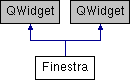
\includegraphics[height=2.000000cm]{classFinestra}
\end{center}
\end{figure}
\subsubsection*{Public Member Functions}
\begin{DoxyCompactItemize}
\item 
{\bfseries Finestra} (Q\+Widget $\ast$parent=0, const char $\ast$name=0)\hypertarget{classFinestra_a8ec00c73de692c63ac3cc1ff48cf1150}{}\label{classFinestra_a8ec00c73de692c63ac3cc1ff48cf1150}

\item 
void {\bfseries Data\+File} (char $\ast$$\ast$argv, int $\ast$File\+List, int N\+F\+Ile)\hypertarget{classFinestra_a0350b9437e10e751a3e55be68ca552ff}{}\label{classFinestra_a0350b9437e10e751a3e55be68ca552ff}

\item 
void {\bfseries Conf\+File} (char $\ast$File\+Name)\hypertarget{classFinestra_a418fd69a796855fc20dcdaf6bb94fc68}{}\label{classFinestra_a418fd69a796855fc20dcdaf6bb94fc68}

\item 
{\bfseries Finestra} (Q\+Widget $\ast$parent=0, const char $\ast$name=0)\hypertarget{classFinestra_a8ec00c73de692c63ac3cc1ff48cf1150}{}\label{classFinestra_a8ec00c73de692c63ac3cc1ff48cf1150}

\end{DoxyCompactItemize}


\subsubsection{Detailed Description}
Defines a window. 

Definition at line 362 of file Elementi\+Grafici.\+h.



The documentation for this class was generated from the following files\+:\begin{DoxyCompactItemize}
\item 
src/\+Avvis/Elementi\+Grafici.\+h\item 
src/\+Avvis/main.\+cpp\item 
src/\+Avvis/Finestra.\+cpp\end{DoxyCompactItemize}

\hypertarget{structFORCES}{}\subsection{F\+O\+R\+C\+ES Struct Reference}
\label{structFORCES}\index{F\+O\+R\+C\+ES@{F\+O\+R\+C\+ES}}


Single contribution of the forces.  




{\ttfamily \#include $<$Forces.\+h$>$}

\subsubsection*{Public Attributes}
\begin{DoxyCompactItemize}
\item 
double \hyperlink{structFORCES_ac77c91979738079508cf3f257a7164ba}{Dir} \mbox{[}3\mbox{]}\hypertarget{structFORCES_ac77c91979738079508cf3f257a7164ba}{}\label{structFORCES_ac77c91979738079508cf3f257a7164ba}

\begin{DoxyCompactList}\small\item\em Direction. \end{DoxyCompactList}\item 
double \hyperlink{structFORCES_a034ef504c45f9a730ddb6053df710a38}{Ext} \mbox{[}3\mbox{]}\hypertarget{structFORCES_a034ef504c45f9a730ddb6053df710a38}{}\label{structFORCES_a034ef504c45f9a730ddb6053df710a38}

\begin{DoxyCompactList}\small\item\em External. \end{DoxyCompactList}\end{DoxyCompactItemize}


\subsubsection{Detailed Description}
Single contribution of the forces. 

Definition at line 176 of file Forces.\+h.



The documentation for this struct was generated from the following file\+:\begin{DoxyCompactItemize}
\item 
src/\+Addyn/Forces.\+h\end{DoxyCompactItemize}

\hypertarget{classForces}{\subsection{\-Forces \-Class \-Reference}
\label{classForces}\index{\-Forces@{\-Forces}}
}


\-This class performs the different steps to solve the equations of motion via molecular dynamics simulation, simple grancanonical simulation in \-Monte \-Carlo and solution of 1d differential equations.  




{\ttfamily \#include $<$\-Forces.\-h$>$}

\-Inheritance diagram for \-Forces\-:\begin{figure}[H]
\begin{center}
\leavevmode
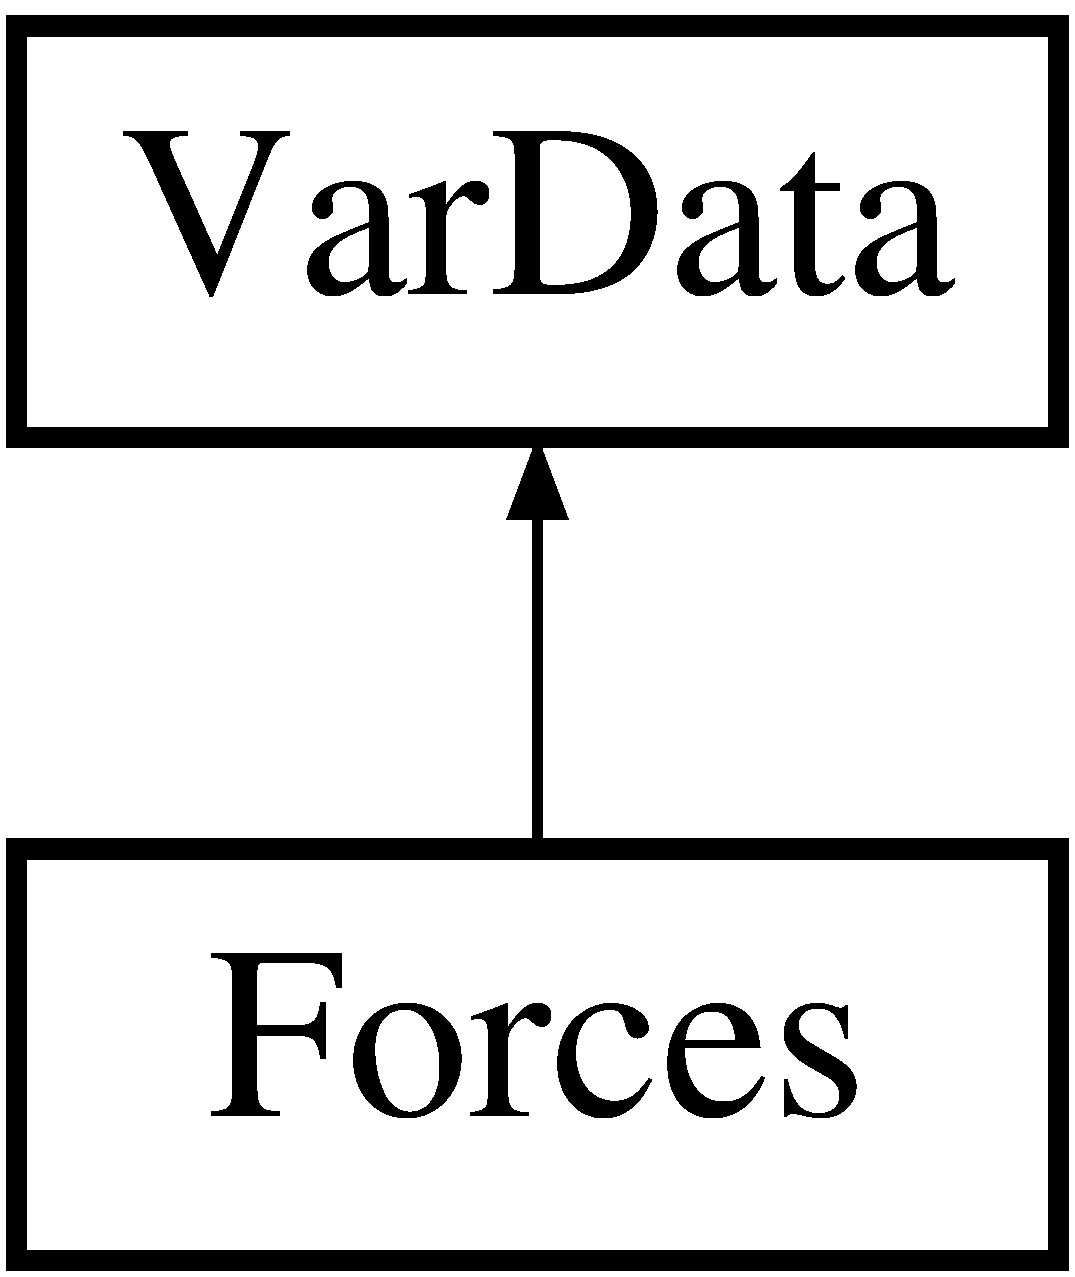
\includegraphics[height=2.000000cm]{classForces}
\end{center}
\end{figure}
\subsubsection*{\-Public \-Types}
\begin{DoxyCompactItemize}
\item 
\hypertarget{classForces_a7cc9ca7ba348e21f2e8597fc07969a51}{typedef void(\-Forces\-::$\ast$ \hyperlink{classForces_a7cc9ca7ba348e21f2e8597fc07969a51}{\-C\-A\-L\-C\-\_\-\-T\-H\-E\-R\-M} )()}\label{classForces_a7cc9ca7ba348e21f2e8597fc07969a51}

\begin{DoxyCompactList}\small\item\em \-Pointer type to the potential function. \end{DoxyCompactList}\item 
\hypertarget{classForces_ae3f1140396007efe5fb7ca46884892eb}{typedef double(\-Forces\-::$\ast$ \hyperlink{classForces_ae3f1140396007efe5fb7ca46884892eb}{\-T\-E\-N\-S\-\_\-\-R\-E\-F} )(double $\ast$\-Pos1, double $\ast$\-Pos2, double $\ast$\-Pos\-P1, double $\ast$\-Pos\-P2)}\label{classForces_ae3f1140396007efe5fb7ca46884892eb}

\begin{DoxyCompactList}\small\item\em \-Data type for distance/field functions. \end{DoxyCompactList}\end{DoxyCompactItemize}
\subsubsection*{\-Public \-Member \-Functions}
\begin{DoxyCompactItemize}
\item 
\hypertarget{classForces_a0b40ef47e7e825a72223abc459561c10}{\hyperlink{classForces_a0b40ef47e7e825a72223abc459561c10}{\-Forces} (int argc, char $\ast$$\ast$argv, int \-N\-Part, char $\ast$\-Conf\-File)}\label{classForces_a0b40ef47e7e825a72223abc459561c10}

\begin{DoxyCompactList}\small\item\em \-Create an initial system and choose the simulation thecnique. \end{DoxyCompactList}\item 
\hypertarget{classForces_abbcd2fc791d4ded94db5172ef1000e42}{\hyperlink{classForces_abbcd2fc791d4ded94db5172ef1000e42}{\-Forces} (int argc, char $\ast$$\ast$argv, char $\ast$\-Conf\-File\-Ext, char $\ast$\-Snapshot)}\label{classForces_abbcd2fc791d4ded94db5172ef1000e42}

\begin{DoxyCompactList}\small\item\em \-Read an initial system and choose the simulation thecnique. \end{DoxyCompactList}\item 
\hypertarget{classForces_ac11429f7ec42e6eb4806e77f8aa24e7f}{void \hyperlink{classForces_ac11429f7ec42e6eb4806e77f8aa24e7f}{\-Shout} (const char $\ast$s,...)}\label{classForces_ac11429f7ec42e6eb4806e77f8aa24e7f}

\begin{DoxyCompactList}\small\item\em \-Internal message. \end{DoxyCompactList}\item 
\hypertarget{classForces_aa7040ce5b212b067b9edc0e48966f593}{void \hyperlink{classForces_aa7040ce5b212b067b9edc0e48966f593}{\-Alloc\-Method} ()}\label{classForces_aa7040ce5b212b067b9edc0e48966f593}

\begin{DoxyCompactList}\small\item\em \-Allocated the structures needed for the corresponding simulation method. \end{DoxyCompactList}\item 
\hypertarget{classForces_a053a9be7328b6a532baf8774f8479188}{void \hyperlink{classForces_a053a9be7328b6a532baf8774f8479188}{\-Prepare\-Sys} ()}\label{classForces_a053a9be7328b6a532baf8774f8479188}

\begin{DoxyCompactList}\small\item\em \-Calculate some initial quantities for the succesive calculations. \end{DoxyCompactList}\item 
\hypertarget{classForces_afb0db3e5d9d3ca56511f4942b695a33c}{void \hyperlink{classForces_afb0db3e5d9d3ca56511f4942b695a33c}{\-Prepare\-Parallel} (int argc, char $\ast$$\ast$argv)}\label{classForces_afb0db3e5d9d3ca56511f4942b695a33c}

\begin{DoxyCompactList}\small\item\em \-Create the grid for the parallelisation. \end{DoxyCompactList}\item 
\hypertarget{classForces_ad23deb6f28e0c4e08e69556f04028e82}{\hyperlink{classForces_ad23deb6f28e0c4e08e69556f04028e82}{$\sim$\-Forces} ()}\label{classForces_ad23deb6f28e0c4e08e69556f04028e82}

\begin{DoxyCompactList}\small\item\em \-Frees the memory. \end{DoxyCompactList}\item 
\hypertarget{classForces_a632d50bc6acb5d08614d0f99a7ed7293}{void \hyperlink{classForces_a632d50bc6acb5d08614d0f99a7ed7293}{\-Info} ()}\label{classForces_a632d50bc6acb5d08614d0f99a7ed7293}

\begin{DoxyCompactList}\small\item\em \-System's info. \end{DoxyCompactList}\item 
\hypertarget{classForces_a54e451b95d534ac661b873f7c5773435}{int \hyperlink{classForces_a54e451b95d534ac661b873f7c5773435}{\-Read\-Conf\-Dinamica} (char $\ast$\-File)}\label{classForces_a54e451b95d534ac661b873f7c5773435}

\begin{DoxyCompactList}\small\item\em \-Read the config file. \end{DoxyCompactList}\item 
\hypertarget{classForces_a2d9aa5d817b97aecdc4dc418d1be255c}{void \hyperlink{classForces_a2d9aa5d817b97aecdc4dc418d1be255c}{\-Init\-Const} ()}\label{classForces_a2d9aa5d817b97aecdc4dc418d1be255c}

\begin{DoxyCompactList}\small\item\em \-Read the config file. \end{DoxyCompactList}\item 
\hypertarget{classForces_a2bd0476e620e68ae04990018f4520bf6}{int \hyperlink{classForces_a2bd0476e620e68ae04990018f4520bf6}{\-Re\-Set\-N\-Part} (int \-New\-N\-Part)}\label{classForces_a2bd0476e620e68ae04990018f4520bf6}

\begin{DoxyCompactList}\small\item\em \-Realloc the number of particles. \end{DoxyCompactList}\item 
\hypertarget{classForces_a935982eadb27b11f47553c06e7aa77ba}{int \hyperlink{classForces_a935982eadb27b11f47553c06e7aa77ba}{\-Re\-Set\-N\-Chain} (int \-New\-N\-Chain)}\label{classForces_a935982eadb27b11f47553c06e7aa77ba}

\begin{DoxyCompactList}\small\item\em \-Realloc the number of chains. \end{DoxyCompactList}\item 
\hypertarget{classForces_aa95d72aa125333d83e91047bc8f4319a}{void \hyperlink{classForces_aa95d72aa125333d83e91047bc8f4319a}{\-Re\-Set\-N\-P\-Ch} (int \-New\-N\-P\-Ch)}\label{classForces_aa95d72aa125333d83e91047bc8f4319a}

\begin{DoxyCompactList}\small\item\em \-Set a new number of particle per chain. \end{DoxyCompactList}\item 
\hypertarget{classForces_a3f36144668126bc6bb1c682c5b10b300}{void \hyperlink{classForces_a3f36144668126bc6bb1c682c5b10b300}{\-Re\-Open} (char $\ast$\-F\-Name, int \-Bf)}\label{classForces_a3f36144668126bc6bb1c682c5b10b300}

\begin{DoxyCompactList}\small\item\em \-Open a new file. \end{DoxyCompactList}\item 
\hypertarget{classForces_a5d2e87f58183d51c11ed77483b0d8b4f}{void \hyperlink{classForces_a5d2e87f58183d51c11ed77483b0d8b4f}{\-Fill\-Matrix} ()}\label{classForces_a5d2e87f58183d51c11ed77483b0d8b4f}

\begin{DoxyCompactList}\small\item\em \-Fill the entries of the interaction matrix. \end{DoxyCompactList}\item 
void \hyperlink{classForces_a5404beae7f264277208ee9e55cbea66e}{\-Study\-Sys} ()
\begin{DoxyCompactList}\small\item\em \-Obtain informations for a better performance in inserting the chains. \end{DoxyCompactList}\item 
\hypertarget{classForces_ad3b093268ba213a56fd6350ad4c861f2}{int \hyperlink{classForces_ad3b093268ba213a56fd6350ad4c861f2}{\-Min\-Helfrich} ()}\label{classForces_ad3b093268ba213a56fd6350ad4c861f2}

\begin{DoxyCompactList}\small\item\em \-Minimum of the \-Helfrich \-Hamiltonian. \end{DoxyCompactList}\item 
\hypertarget{classForces_affd222b3ce256a0c538341cc4d81865e}{int \hyperlink{classForces_affd222b3ce256a0c538341cc4d81865e}{\-Dyn\-Integration} ()}\label{classForces_affd222b3ce256a0c538341cc4d81865e}

\begin{DoxyCompactList}\small\item\em \-Boh. \end{DoxyCompactList}\item 
\hypertarget{classForces_a338adbdaecf3f72150ce3e88ec710bf1}{void \hyperlink{classForces_a338adbdaecf3f72150ce3e88ec710bf1}{\-Dynamics} ()}\label{classForces_a338adbdaecf3f72150ce3e88ec710bf1}

\begin{DoxyCompactList}\small\item\em \-Sum up all the forces and update the positions. \end{DoxyCompactList}\item 
void \hyperlink{classForces_a941bab4d0655ea3e774cd525e664be52}{\-Solve} ()
\begin{DoxyCompactList}\small\item\em \-Solve a system of four oder differential equation. \end{DoxyCompactList}\item 
void \hyperlink{classForces_ac6b917be683f5ceaeec62edbf9472511}{\-Solve\-Links} ()
\begin{DoxyCompactList}\small\item\em \-Solve a system of four oder differential equation of particles connected by links. \end{DoxyCompactList}\item 
\hypertarget{classForces_a35266508f74e6ca08000446ebbd62fc6}{void \hyperlink{classForces_a35266508f74e6ca08000446ebbd62fc6}{\-Solve\-Links\-Sparse} ()}\label{classForces_a35266508f74e6ca08000446ebbd62fc6}

\begin{DoxyCompactList}\small\item\em \-Solve a system of four oder differential equation of particles connected by links. \end{DoxyCompactList}\item 
void \hyperlink{classForces_abcac13d7754b73f6f22b2900a0d46d7d}{\-Solve\-Links\-Iterative} ()
\begin{DoxyCompactList}\small\item\em \-Solve a system of four oder differential equation of particles connected by links. \end{DoxyCompactList}\item 
void \hyperlink{classForces_a3953ee74479102530a979e3cd447d174}{\-Solve\-Rod} ()
\begin{DoxyCompactList}\small\item\em \-Solve a system of four oder differential equation of particles connected by links. \end{DoxyCompactList}\item 
void \hyperlink{classForces_a7a03a3d52f5a114cbbc22e60af60c049}{\-Solve\-Leaves} ()
\begin{DoxyCompactList}\small\item\em \-Solve a system of four oder differential equation of particles in a line. \end{DoxyCompactList}\item 
\hypertarget{classForces_a02e68a26ce7e19af9d0b729af61e72d3}{int \hyperlink{classForces_a02e68a26ce7e19af9d0b729af61e72d3}{\-Update} ()}\label{classForces_a02e68a26ce7e19af9d0b729af61e72d3}

\begin{DoxyCompactList}\small\item\em \-Boh. \end{DoxyCompactList}\item 
void \hyperlink{classForces_a050e80ecdb61ccf749649d6ec6542ee7}{\-Vel\-Verlet\-Rigid} ()
\begin{DoxyCompactList}\small\item\em \-Velocity \-Verlet for a rigid body, first step. \end{DoxyCompactList}\item 
void \hyperlink{classForces_a3d421e17e32ee064077a14cc483a7c4e}{\-Vel\-Verlet\-Rigid2} ()
\begin{DoxyCompactList}\small\item\em \-Velocity \-Verlet for a rigid body, second step. \end{DoxyCompactList}\item 
int \hyperlink{classForces_a8b42f5fd80b4ad0cbf71649cd58f17ef}{\-If\-Metropolis} (double \-Exp\-Arg, double \-Weight)
\begin{DoxyCompactList}\small\item\em \-Metropolis acceptance criterium. \end{DoxyCompactList}\item 
int \hyperlink{classForces_a105420510a35a5f3ab726a943a279ce4}{\-Insert\-Bead} (int p)
\begin{DoxyCompactList}\small\item\em \-Insert a particle in the box. \end{DoxyCompactList}\item 
void \hyperlink{classForces_ada3b7b85ea783d27acfd5ff27165e4e2}{\-Ignore\-Ch} (int c)
\begin{DoxyCompactList}\small\item\em \-Ignore a chain in the system (densities, pairlist) \end{DoxyCompactList}\item 
void \hyperlink{classForces_a93ffd0cd932626a8b09911f2b3c96e10}{\-Rem\-Ch\-From\-Sys} (int c)
\begin{DoxyCompactList}\small\item\em \-Delete a chain in the system. \end{DoxyCompactList}\item 
void \hyperlink{classForces_a69e06a7f5662a462ed7b67428f1a8e69}{\-Save\-Ch} (int c)
\begin{DoxyCompactList}\small\item\em \-Save the chain configuration. \end{DoxyCompactList}\item 
void \hyperlink{classForces_aaea07c5c698924ba7efc75988997086c}{\-Re\-Insert\-Ch} (int c)
\begin{DoxyCompactList}\small\item\em \-Reinsert the chain in the previous position. \end{DoxyCompactList}\item 
void \hyperlink{classForces_a1c4bc6d5b46ce58c1e6139e9feccea5a}{\-Consider\-Ch} (int c)
\begin{DoxyCompactList}\small\item\em \-Consider a chain in the system (densities, pairlist) \end{DoxyCompactList}\item 
double \hyperlink{classForces_aed7689c1abd36c6ac8743fadd2e6cbdf}{\-Insert\-Ch} (int c)
\begin{DoxyCompactList}\small\item\em \-Displace a chain in the box. \end{DoxyCompactList}\item 
double \hyperlink{classForces_a8e9fda810a12eeaba2c7b72af5a1e664}{\-Insert\-Rest} (int p\-Curr, int \-Start\-Pos)
\begin{DoxyCompactList}\small\item\em \-Build the rest of the chain. \end{DoxyCompactList}\item 
double \hyperlink{classForces_aae7e57b54965ad985ab041a040dfc93d}{\-Remove\-Ch\-Bias} (int c)
\begin{DoxyCompactList}\small\item\em \-Remove a chain in the box. \end{DoxyCompactList}\item 
double \hyperlink{classForces_a766511ed1b66a8b4ef97b1b343fb6254}{\-Insert\-Ch\-Bias} (int c)
\begin{DoxyCompactList}\small\item\em \-Put a chain in the box. \end{DoxyCompactList}\item 
double \hyperlink{classForces_a97d31164f5b192ff0e68d26f120e9e78}{\-Weight\-Set\-Bond} (int p, int t)
\begin{DoxyCompactList}\small\item\em \-Weight a set of bonds for the configurational bias. \end{DoxyCompactList}\item 
double \hyperlink{classForces_ac80c2d5ad9a6b3f4de84f825844d1a36}{\-Create\-Set\-Bond} (int p, int t)
\begin{DoxyCompactList}\small\item\em \-Create a set of bonds for the configurational bias. \end{DoxyCompactList}\item 
int \hyperlink{classForces_aaa86df6dc24f47e52ca153db60bd6749}{\-Move\-Bead} (int p)
\begin{DoxyCompactList}\small\item\em \-Move a particle in the box. \end{DoxyCompactList}\item 
int \hyperlink{classForces_a56709cda842db1c6f3813acc5bca5237}{\-Try\-Insert} ()
\begin{DoxyCompactList}\small\item\em \-Trial insertion. \end{DoxyCompactList}\item 
int \hyperlink{classForces_a0658783c2d6dcab7a875f938747255a6}{\-Try\-Remove} ()
\begin{DoxyCompactList}\small\item\em \-Trial removal. \end{DoxyCompactList}\item 
int \hyperlink{classForces_ad69656acc46a08f2361dbe5b1067dffa}{\-Try\-Move} ()
\begin{DoxyCompactList}\small\item\em \-Trial movement. \end{DoxyCompactList}\item 
int \hyperlink{classForces_aa30016ca75ff4d48a905a9dad7da023f}{\-Try\-Move\-Ch} ()
\begin{DoxyCompactList}\small\item\em \-Trial desplacement of a chain. \end{DoxyCompactList}\item 
int \hyperlink{classForces_ab7bfa9d7122c69b311f666740653bd0b}{\-Try\-Insert\-Ch} ()
\begin{DoxyCompactList}\small\item\em \-Trial insertion of a chain. \end{DoxyCompactList}\item 
int \hyperlink{classForces_aefc3ccff8a9805e952ddc49194595844}{\-Try\-Remove\-Ch} ()
\begin{DoxyCompactList}\small\item\em \-Trial removal of a chain. \end{DoxyCompactList}\item 
int \hyperlink{classForces_a949d9de0a157e4258f88d5b5f322f74e}{\-Try\-Insert\-Ch\-Bias} ()
\begin{DoxyCompactList}\small\item\em \-Trial biased insertion of a chain. \end{DoxyCompactList}\item 
int \hyperlink{classForces_a32c3f4b656bce2cf73370ce605f53113}{\-Try\-Remove\-Ch\-Bias} ()
\begin{DoxyCompactList}\small\item\em \-Trial biased removal of a chain. \end{DoxyCompactList}\item 
void \hyperlink{classForces_af9eda9a781eabd31a8813c9a64f2d5ec}{\-Widom\-Insert} (double $\ast$\-Nrg\-Diff)
\begin{DoxyCompactList}\small\item\em \-Widom insertion. \end{DoxyCompactList}\item 
void \hyperlink{classForces_a85d825b7b4af29d476abbf098ce630e3}{\-Widom\-Remove} (double $\ast$\-Nrg\-Diff, int p)
\begin{DoxyCompactList}\small\item\em \-Widom removal. \end{DoxyCompactList}\item 
void \hyperlink{classForces_acffb530559d4e3ebfac6481a46468f52}{\-Widom\-Insert\-Ch} (double $\ast$\-Nrg\-Diff)
\begin{DoxyCompactList}\small\item\em \-Widom insertion. \end{DoxyCompactList}\item 
void \hyperlink{classForces_a0ab84cf7b372ab5ae21966ed671ee4c3}{\-Widom\-Remove\-Ch} (double $\ast$\-Nrg\-Diff, int c)
\begin{DoxyCompactList}\small\item\em \-Widom removal. \end{DoxyCompactList}\item 
void \hyperlink{classForces_af07ae7761f13798c6de1391b10c5856d}{\-Widom\-Bias\-Ch\-In} (double $\ast$\-Weight)
\begin{DoxyCompactList}\small\item\em \-Widom with \-Rosenbluth weight. \end{DoxyCompactList}\item 
void \hyperlink{classForces_ab249c91e15e3611167002159ef6d5b60}{\-Widom\-Bias\-Ch\-Out} (double $\ast$\-Weight, int c)
\begin{DoxyCompactList}\small\item\em \-Widom with \-Rosenbluth weight. \end{DoxyCompactList}\item 
void \hyperlink{classForces_a7a55d93047438c9c5f5f9145a995e8d0}{\-Vel\-Verlet1} ()
\begin{DoxyCompactList}\small\item\em \-First step of the velocity \-Verlet. \end{DoxyCompactList}\item 
void \hyperlink{classForces_a379f6968f484a2a975c657f07821731c}{\-Langevin\-Therm} ()
\begin{DoxyCompactList}\small\item\em \-Langevin thermostat. \end{DoxyCompactList}\item 
void \hyperlink{classForces_a731619cf10a23878480c0af79252ed3e}{\-Andersen\-Therm} ()
\begin{DoxyCompactList}\small\item\em \-Andersen thermostat. \end{DoxyCompactList}\item 
void \hyperlink{classForces_a795803d47c68fef34839e68ffb2de60e}{\-Berendsen\-Therm} ()
\begin{DoxyCompactList}\small\item\em \-Berendsen thermostat. \end{DoxyCompactList}\item 
\hypertarget{classForces_ae11de37aafa6549029bdf20e36bee7f4}{void \hyperlink{classForces_ae11de37aafa6549029bdf20e36bee7f4}{\-No\-Therm} ()}\label{classForces_ae11de37aafa6549029bdf20e36bee7f4}

\begin{DoxyCompactList}\small\item\em \-No thermostat. \end{DoxyCompactList}\item 
void \hyperlink{classForces_a7965b2207a6253f8215b96a7195cb5bc}{\-Vel\-Verlet2} ()
\begin{DoxyCompactList}\small\item\em \-Second step of the velocity \-Verlet. \end{DoxyCompactList}\item 
void \hyperlink{classForces_a8de191a7e9bb4c04ea140023c0bffaba}{\-Choose\-Thermostat} (int \-Mode)
\begin{DoxyCompactList}\small\item\em \-Choose a calculation mode. \end{DoxyCompactList}\item 
\hypertarget{classForces_a0ccf73fded29832c9d6c8edad5a51b76}{void \hyperlink{classForces_a0ccf73fded29832c9d6c8edad5a51b76}{\-Apply\-Therm} ()}\label{classForces_a0ccf73fded29832c9d6c8edad5a51b76}

\begin{DoxyCompactList}\small\item\em \-Pointer to the energy function. \end{DoxyCompactList}\item 
int \hyperlink{classForces_abe46a6cf819d53f35747565f9276854f}{\-Force\-Field\-Line} ()
\begin{DoxyCompactList}\small\item\em \-Helfrich \-Hamiltonian for a line. \end{DoxyCompactList}\item 
\hypertarget{classForces_aad7c51f4a67ea41983881db33d1e5434}{int \hyperlink{classForces_aad7c51f4a67ea41983881db33d1e5434}{\-Sum\-Some\-Forces} (int \-How\-Many)}\label{classForces_aad7c51f4a67ea41983881db33d1e5434}

\begin{DoxyCompactList}\small\item\em \-Boh. \end{DoxyCompactList}\item 
int \hyperlink{classForces_aed97e42cbfeb918574e91a90719864ab}{\-Force\-Field\-Leaves} ()
\begin{DoxyCompactList}\small\item\em \-Helfrich \-Hamiltonian with an elastic coupling. \end{DoxyCompactList}\item 
int \hyperlink{classForces_aa57796d41906bf35c6a79225ecda6f98}{\-Force\-Field\-Bulk} ()
\begin{DoxyCompactList}\small\item\em \-Armonic potential on a lattice. \end{DoxyCompactList}\item 
void \hyperlink{classForces_ae35380222f8a3cacfa4a4df6d1742ffb}{\-Force\-Field\-Rod} ()
\begin{DoxyCompactList}\small\item\em \-Bending potential on a rod. \end{DoxyCompactList}\item 
\hypertarget{classForces_a8f12492ed75d05c816d8f14bbeaf71be}{void \hyperlink{classForces_a8f12492ed75d05c816d8f14bbeaf71be}{\-Force\-Field\-Rigid} ()}\label{classForces_a8f12492ed75d05c816d8f14bbeaf71be}

\begin{DoxyCompactList}\small\item\em \-Interaction between rigid bodies. \end{DoxyCompactList}\item 
\hypertarget{classForces_a5c32ef207ba714e72e72de3063860b39}{void \hyperlink{classForces_a5c32ef207ba714e72e72de3063860b39}{\-Calc\-Forces\-Dens\-Func} ()}\label{classForces_a5c32ef207ba714e72e72de3063860b39}

\begin{DoxyCompactList}\small\item\em \-Calculate the forces for the density functional. \end{DoxyCompactList}\item 
\hypertarget{classForces_a7b92a25206538d578d6129879bfac183}{void \hyperlink{classForces_a7b92a25206538d578d6129879bfac183}{\-Print\-Force} ()}\label{classForces_a7b92a25206538d578d6129879bfac183}

\begin{DoxyCompactList}\small\item\em \-Print the force and the potential. \end{DoxyCompactList}\item 
\hypertarget{classForces_a68e26f1fe45d8de3362c59de39ddcbc9}{void \hyperlink{classForces_a68e26f1fe45d8de3362c59de39ddcbc9}{\-Get\-Force\-Field} ()}\label{classForces_a68e26f1fe45d8de3362c59de39ddcbc9}

\begin{DoxyCompactList}\small\item\em \-Calculate the force field summing every single contribution. \end{DoxyCompactList}\item 
\hypertarget{classForces_ab7b56f14cb877cece5075bc6a160aab3}{void \hyperlink{classForces_ab7b56f14cb877cece5075bc6a160aab3}{\-Tab\-Force\-Alloc} (int \-N\-Tab\-Ext)}\label{classForces_ab7b56f14cb877cece5075bc6a160aab3}

\begin{DoxyCompactList}\small\item\em \-Tabulate the values of the force. \end{DoxyCompactList}\item 
\hypertarget{classForces_a1c00d241ca805ba05becca0e9aafe45f}{void \hyperlink{classForces_a1c00d241ca805ba05becca0e9aafe45f}{\-Tab\-Pot} ()}\label{classForces_a1c00d241ca805ba05becca0e9aafe45f}

\begin{DoxyCompactList}\small\item\em \-Tabulate the values of the potential. \end{DoxyCompactList}\item 
\hypertarget{classForces_ac56bd243d0c3cac921959104fac03d2c}{void \hyperlink{classForces_ac56bd243d0c3cac921959104fac03d2c}{\-Nano\-Interaction} ()}\label{classForces_ac56bd243d0c3cac921959104fac03d2c}

\begin{DoxyCompactList}\small\item\em \-Calculate all the interaction with the nano. \end{DoxyCompactList}\item 
\hypertarget{classForces_a7ab5c0bcf11c3f33530a25984720b424}{double \hyperlink{classForces_a7ab5c0bcf11c3f33530a25984720b424}{\-Nano\-Nrg} (int p)}\label{classForces_a7ab5c0bcf11c3f33530a25984720b424}

\begin{DoxyCompactList}\small\item\em \-Exchange energy with the nano. \end{DoxyCompactList}\item 
\hypertarget{classForces_af2058d93db6e3ef4894d33f6790a6749}{double \hyperlink{classForces_af2058d93db6e3ef4894d33f6790a6749}{\-Nano\-Nrg} (double $\ast$\-Pos, int t)}\label{classForces_af2058d93db6e3ef4894d33f6790a6749}

\begin{DoxyCompactList}\small\item\em \-Exchange energy with the nano. \end{DoxyCompactList}\item 
\hypertarget{classForces_ad7e01b1bd04ce252d991ae872eaa5270}{void \hyperlink{classForces_ad7e01b1bd04ce252d991ae872eaa5270}{\-Def\-Force\-Param} ()}\label{classForces_ad7e01b1bd04ce252d991ae872eaa5270}

\begin{DoxyCompactList}\small\item\em \-Define the parameters for calculating the force. \end{DoxyCompactList}\item 
\hypertarget{classForces_ae1187ff72e7ad2765b17948df1aff2b4}{void \hyperlink{classForces_ae1187ff72e7ad2765b17948df1aff2b4}{\-Def\-Nano\-Force\-Param} ()}\label{classForces_ae1187ff72e7ad2765b17948df1aff2b4}

\begin{DoxyCompactList}\small\item\em \-Define the parameters for calculating the force. \end{DoxyCompactList}\item 
\hypertarget{classForces_a299061ca48b352b4d40c0dfbb6ffd2da}{double \hyperlink{classForces_a299061ca48b352b4d40c0dfbb6ffd2da}{\-Rigid\-L\-J} (int n\-Nano, double \-Dist, double $\ast$\-Pot, double \-Sign)}\label{classForces_a299061ca48b352b4d40c0dfbb6ffd2da}

\begin{DoxyCompactList}\small\item\em \-Force between to rigid bodies. \end{DoxyCompactList}\item 
double \hyperlink{classForces_abd9350bc451b7ae5507675805b4318d5}{\-Rigid\-Hamaker} (int n, double \-Dist, double $\ast$\-Pot, double \-Sign)
\begin{DoxyCompactList}\small\item\em \-Hamaker potential. \end{DoxyCompactList}\item 
\hypertarget{classForces_af8f6e965e516633b54115556243a681a}{double \hyperlink{classForces_af8f6e965e516633b54115556243a681a}{\-Rigid\-Coulomb} (int n\-Nano, double \-Dist, double $\ast$\-Pot, double \-Sign)}\label{classForces_af8f6e965e516633b54115556243a681a}

\begin{DoxyCompactList}\small\item\em \-Force between to rigid bodies. \end{DoxyCompactList}\item 
\hypertarget{classForces_a4aa4b64aa78c004e13b7d5e059c61c7f}{double \hyperlink{classForces_a4aa4b64aa78c004e13b7d5e059c61c7f}{\-Rigid\-Distance\-Rad} (int n, int nn, double $\ast$dr)}\label{classForces_a4aa4b64aa78c004e13b7d5e059c61c7f}

\begin{DoxyCompactList}\small\item\em \-Distance between two bodies. \end{DoxyCompactList}\item 
\hypertarget{classForces_a0bd8b1fc300bbbf7b4d7a6c5836ff0dc}{double \hyperlink{classForces_a0bd8b1fc300bbbf7b4d7a6c5836ff0dc}{\-Rigid\-Distance\-Axis} (int n, int nn, double $\ast$dr)}\label{classForces_a0bd8b1fc300bbbf7b4d7a6c5836ff0dc}

\begin{DoxyCompactList}\small\item\em \-Distance between two bodies. \end{DoxyCompactList}\item 
\hypertarget{classForces_a0d76b871ebe7ef570ef9c2fcba03ddb8}{void {\bfseries \-Point\-Shape} (int i\-Shape)}\label{classForces_a0d76b871ebe7ef570ef9c2fcba03ddb8}

\item 
\hypertarget{classForces_af449f7871a4d5c5f1e263e4fe660bd63}{double \hyperlink{classForces_af449f7871a4d5c5f1e263e4fe660bd63}{\-Harmonic} (double \-Dist2, int t1, int t2, double $\ast$\-Pot)}\label{classForces_af449f7871a4d5c5f1e263e4fe660bd63}

\begin{DoxyCompactList}\small\item\em \-Harmonic potential. \end{DoxyCompactList}\item 
\hypertarget{classForces_a1f0b019b2a8c81938b8f4a3f3ddcfc48}{double \hyperlink{classForces_a1f0b019b2a8c81938b8f4a3f3ddcfc48}{\-Step\-Pot} (double \-Dist2, int t1, int t2, double $\ast$\-Pot)}\label{classForces_a1f0b019b2a8c81938b8f4a3f3ddcfc48}

\begin{DoxyCompactList}\small\item\em \-Step potential. \end{DoxyCompactList}\item 
\hypertarget{classForces_ad1ef4b910c2f6e057b8b2e079d32100b}{double \hyperlink{classForces_ad1ef4b910c2f6e057b8b2e079d32100b}{\-Electro\-Pot} (double \-Dist2, int t1, int t2, double $\ast$\-Pot)}\label{classForces_ad1ef4b910c2f6e057b8b2e079d32100b}

\begin{DoxyCompactList}\small\item\em \-Potential for the electrical lines. \end{DoxyCompactList}\item 
\hypertarget{classForces_a28fd299b40762b1703462b830df2473d}{double \hyperlink{classForces_a28fd299b40762b1703462b830df2473d}{\-L\-J39} (double \-Dist2, int t1, int t2, double $\ast$\-Pot)}\label{classForces_a28fd299b40762b1703462b830df2473d}

\begin{DoxyCompactList}\small\item\em \-Integrated \-Lennard \-Jones potential. \end{DoxyCompactList}\item 
\hypertarget{classForces_ad6b11a62ba4f9871d598109fe007a121}{double \hyperlink{classForces_ad6b11a62ba4f9871d598109fe007a121}{\-L\-J\-Pot} (double \-Dist2, int t1, int t2, double $\ast$\-Pot)}\label{classForces_ad6b11a62ba4f9871d598109fe007a121}

\begin{DoxyCompactList}\small\item\em \-Classical \-Lennard \-Jones potential. \end{DoxyCompactList}\item 
\hypertarget{classForces_ac5ef477f97601b779392b8622ac6b1fe}{double \hyperlink{classForces_ac5ef477f97601b779392b8622ac6b1fe}{\-Potential} (double \-Dist, int t1, int t2, double $\ast$\-Pot)}\label{classForces_ac5ef477f97601b779392b8622ac6b1fe}

\begin{DoxyCompactList}\small\item\em \-Pointer to a potential. \end{DoxyCompactList}\item 
double \hyperlink{classForces_a59c5e973ca9b852115683c3cc2fc6035}{\-Calc\-Tot\-Nrg\-Ch} ()
\begin{DoxyCompactList}\small\item\em \-Calculate and sum up the energy of the chains. \end{DoxyCompactList}\item 
double \hyperlink{classForces_a279acbc4a6538860aad95a08f3edc78f}{\-Calc\-Tot\-Nrg\-Bead} ()
\begin{DoxyCompactList}\small\item\em \-Calculate and sum up the energy of the part. \end{DoxyCompactList}\item 
\hypertarget{classForces_a3fa7f92932bea2b6abd0231b7610b6d2}{double \hyperlink{classForces_a3fa7f92932bea2b6abd0231b7610b6d2}{\-Calc\-Nrg\-Bead} (int p, double $\ast$\-Pot)}\label{classForces_a3fa7f92932bea2b6abd0231b7610b6d2}

\begin{DoxyCompactList}\small\item\em \-Pointer to the energy function. \end{DoxyCompactList}\item 
\hypertarget{classForces_ac028948e0862f18bf805f23078ebf7fa}{double \hyperlink{classForces_ac028948e0862f18bf805f23078ebf7fa}{\-Calc\-Nrg\-Ch} (int c, double $\ast$\-Pot)}\label{classForces_ac028948e0862f18bf805f23078ebf7fa}

\begin{DoxyCompactList}\small\item\em \-Pointer to the chain energy function. \end{DoxyCompactList}\item 
double \hyperlink{classForces_ab282af6b6987c94833eb3eb9bc5d28a4}{\-Nrg\-Ch\-Bond\-Dens} (int c, double $\ast$\-Pot)
\begin{DoxyCompactList}\small\item\em \-Calculate the bond and the density functional energies. \end{DoxyCompactList}\item 
\hypertarget{classForces_ab40568d4784987cff90e5081eee86a93}{double \hyperlink{classForces_ab40568d4784987cff90e5081eee86a93}{\-Nrg\-Ch\-Dens} (int c, double $\ast$\-Pot)}\label{classForces_ab40568d4784987cff90e5081eee86a93}

\begin{DoxyCompactList}\small\item\em \-Calculate the density functional energies. \end{DoxyCompactList}\item 
\hypertarget{classForces_abcf9fe5fd43b953a9f9c836bb23f4b26}{double \hyperlink{classForces_abcf9fe5fd43b953a9f9c836bb23f4b26}{\-Calc\-Pairwise} (int p, double $\ast$\-Pot)}\label{classForces_abcf9fe5fd43b953a9f9c836bb23f4b26}

\begin{DoxyCompactList}\small\item\em \-Calculate the non bonded interaction energy with the neighbouring particles. \end{DoxyCompactList}\item 
\hypertarget{classForces_ad5fa9268736b6a2b17b8b600fea178be}{double \hyperlink{classForces_ad5fa9268736b6a2b17b8b600fea178be}{\-Calc\-Pairwise\-Ch} (int c, double $\ast$\-Pot)}\label{classForces_ad5fa9268736b6a2b17b8b600fea178be}

\begin{DoxyCompactList}\small\item\em \-Calculate the non bonded interaction energy with the neighbouring particles. \end{DoxyCompactList}\item 
\hypertarget{classForces_a85c318f4f79eb537a5d0be2552fae2af}{double \hyperlink{classForces_a85c318f4f79eb537a5d0be2552fae2af}{\-Calc\-Bending} (int p)}\label{classForces_a85c318f4f79eb537a5d0be2552fae2af}

\begin{DoxyCompactList}\small\item\em \-Calculate the bonded interaction energy with the neighbouring particles. \end{DoxyCompactList}\item 
\hypertarget{classForces_a9695c7258e7d8a3fb781280f258747cf}{double \hyperlink{classForces_a9695c7258e7d8a3fb781280f258747cf}{\-Calc\-Spring} (int p)}\label{classForces_a9695c7258e7d8a3fb781280f258747cf}

\begin{DoxyCompactList}\small\item\em \-Calculate the spring interaction energy with the neighbouring particles. \end{DoxyCompactList}\item 
double \hyperlink{classForces_adb6d3708682daf3cc9dd70081adfb894}{\-Calc\-Bonded} (int p, double $\ast$\-Pot)
\begin{DoxyCompactList}\small\item\em \-Calculate the spring and the bonded interactions with the other monomers in the chain. \end{DoxyCompactList}\item 
double \hyperlink{classForces_a2ba180156b26af3e2eea135743275fa9}{\-Calc\-Bending\-Ghost} (double $\ast$\-Pos, int p\-Ext)
\begin{DoxyCompactList}\small\item\em \-Calculate the bending energy for a ghost particle. \end{DoxyCompactList}\item 
\hypertarget{classForces_a6fec1e71c9031503f3f3b7a4f4851319}{double \hyperlink{classForces_a6fec1e71c9031503f3f3b7a4f4851319}{\-Calc\-Bonded\-Ch} (int c, double $\ast$\-Pot)}\label{classForces_a6fec1e71c9031503f3f3b7a4f4851319}

\begin{DoxyCompactList}\small\item\em \-Calculate the bonded and spring interaction in a cell. \end{DoxyCompactList}\item 
\hypertarget{classForces_a616546bdad154256f89f9eee067e8166}{void \hyperlink{classForces_a616546bdad154256f89f9eee067e8166}{\-Calc\-Nrg\-Bead\-Dens\-Func} ()}\label{classForces_a616546bdad154256f89f9eee067e8166}

\begin{DoxyCompactList}\small\item\em \-Calculate the spring, bending and non bonded interactions and write it in \-Old\-Nrg\-Pm. \end{DoxyCompactList}\item 
double \hyperlink{classForces_ab18a8becb1983fc28fbeadea39623079}{\-Calc\-Nrg\-Bead\-Dens\-Func} (int p, double $\ast$\-Pot)
\begin{DoxyCompactList}\small\item\em \-Calculate the spring, bending and non bonded interactions. \end{DoxyCompactList}\item 
double \hyperlink{classForces_a2595efd4257201b5b7c30c73086f94c3}{\-Check\-Dom\-Dec} (int p)
\begin{DoxyCompactList}\small\item\em \-Check if all the particles are taken in account. \end{DoxyCompactList}\item 
\hypertarget{classForces_a419ca9dee6d5e955abe44cf409e24d66}{void \hyperlink{classForces_a419ca9dee6d5e955abe44cf409e24d66}{\-Check\-Pair\-List} ()}\label{classForces_a419ca9dee6d5e955abe44cf409e24d66}

\begin{DoxyCompactList}\small\item\em \-Check the pair list. \end{DoxyCompactList}\item 
\hypertarget{classForces_a791c1d5f301eb9c0d39c43a180eaf737}{double \hyperlink{classForces_a791c1d5f301eb9c0d39c43a180eaf737}{\-Sum\-Forces\-M\-D} ()}\label{classForces_a791c1d5f301eb9c0d39c43a180eaf737}

\begin{DoxyCompactList}\small\item\em \-Iterate all over the particles and calculate the forces. \end{DoxyCompactList}\item 
\hypertarget{classForces_a5c95469e44bbbea88c38809308ca4551}{double \hyperlink{classForces_a5c95469e44bbbea88c38809308ca4551}{\-Wei3} (const double r, const double a)}\label{classForces_a5c95469e44bbbea88c38809308ca4551}

\begin{DoxyCompactList}\small\item\em \-Cubic weighting function. \end{DoxyCompactList}\item 
\hypertarget{classForces_a3d44e49e6ced82a300d6071060b72c48}{double \hyperlink{classForces_a3d44e49e6ced82a300d6071060b72c48}{\-Der\-Wei3} (const double r, const double a)}\label{classForces_a3d44e49e6ced82a300d6071060b72c48}

\begin{DoxyCompactList}\small\item\em \-Derivative of the cubic weighting function. \end{DoxyCompactList}\item 
\hypertarget{classForces_a2a275bbffe53c778eb8d535f3dc601f8}{double \hyperlink{classForces_a2a275bbffe53c778eb8d535f3dc601f8}{\-Wei2} (const double r, const double b)}\label{classForces_a2a275bbffe53c778eb8d535f3dc601f8}

\begin{DoxyCompactList}\small\item\em \-Quadratic weighting function. \end{DoxyCompactList}\item 
\hypertarget{classForces_a5c07d0e26deb83592ec816a9d6dfd05b}{double \hyperlink{classForces_a5c07d0e26deb83592ec816a9d6dfd05b}{\-Der\-Wei2} (const double r, const double b)}\label{classForces_a5c07d0e26deb83592ec816a9d6dfd05b}

\begin{DoxyCompactList}\small\item\em \-Derivative of the quadratic weighting function. \end{DoxyCompactList}\item 
\hypertarget{classForces_a6330de60f8b181b6e7ac68f9cd103f58}{double \hyperlink{classForces_a6330de60f8b181b6e7ac68f9cd103f58}{\-Dens\-Func\-Nrg\-Ghost} (double $\ast$\-Pos, int p1, int t1)}\label{classForces_a6330de60f8b181b6e7ac68f9cd103f58}

\begin{DoxyCompactList}\small\item\em \-Calculation of the energy from the density functional \-Hamiltonian for the ghost particle. \end{DoxyCompactList}\item 
\hypertarget{classForces_a75fb72ed9ede20a211933fe11dabebcf}{double \hyperlink{classForces_a75fb72ed9ede20a211933fe11dabebcf}{\-Dens\-Func\-Nrg\-Ghost\-Internal} (double $\ast$\-Pos, int p1, int t1)}\label{classForces_a75fb72ed9ede20a211933fe11dabebcf}

\begin{DoxyCompactList}\small\item\em \-Calculation of the energy from the density functional \-Hamiltonian for the ghost particle. \end{DoxyCompactList}\item 
\hypertarget{classForces_aaf00acd2a6784650ce2b34f2c802b6c4}{double \hyperlink{classForces_aaf00acd2a6784650ce2b34f2c802b6c4}{\-Dens\-Func\-Nrg\-Bead} (int p1)}\label{classForces_aaf00acd2a6784650ce2b34f2c802b6c4}

\begin{DoxyCompactList}\small\item\em \-Calculation of the energy from the density functional \-Hamiltonian for the particle p1. \end{DoxyCompactList}\item 
double \hyperlink{classForces_ad288fce3211ed5cafbe899b4d3ca08f5}{\-Dens\-Func\-Nrg\-Ch} (int c, double $\ast$\-Pot)
\begin{DoxyCompactList}\small\item\em \-Calculate the energy from the density functional \-Hamiltonian for the chain c. \end{DoxyCompactList}\item 
\hypertarget{classForces_a3d6dfad06fbcd3a6b9f84b2ccd40f1ef}{double \hyperlink{classForces_a3d6dfad06fbcd3a6b9f84b2ccd40f1ef}{\-Dens\-Func\-Nrg\-Ch\-Av} (int c)}\label{classForces_a3d6dfad06fbcd3a6b9f84b2ccd40f1ef}

\begin{DoxyCompactList}\small\item\em \-Calculate the average energy from the density functional \-Hamiltonian for the chain c. \end{DoxyCompactList}\item 
\hypertarget{classForces_a424676c9ec7046ecef5f6df4a4a104e8}{double \hyperlink{classForces_a424676c9ec7046ecef5f6df4a4a104e8}{\-Dens\-Func\-Nrg\-Ch\-Internal} (int c)}\label{classForces_a424676c9ec7046ecef5f6df4a4a104e8}

\begin{DoxyCompactList}\small\item\em \-Calculate the average energy from the density functional \-Hamiltonian for the chain c. \end{DoxyCompactList}\item 
\hypertarget{classForces_ad6b09c65169c95c3aff47220ad8327c6}{double \hyperlink{classForces_ad6b09c65169c95c3aff47220ad8327c6}{\-Dens\-Func\-Nrg\-Sys} ()}\label{classForces_ad6b09c65169c95c3aff47220ad8327c6}

\begin{DoxyCompactList}\small\item\em \-Calculation of the energy from the density functional \-Hamiltonian for the system. \end{DoxyCompactList}\item 
\hypertarget{classForces_af84f3585b204886f9166af82c0a229ac}{void \hyperlink{classForces_af84f3585b204886f9166af82c0a229ac}{\-Calc\-Dens} (int p\-Init, int p\-End)}\label{classForces_af84f3585b204886f9166af82c0a229ac}

\begin{DoxyCompactList}\small\item\em \-Calculate the local density for the particles between p\-Init and p\-End. \end{DoxyCompactList}\item 
\hypertarget{classForces_a0390d97ed1665851fb6175342d1c598b}{void \hyperlink{classForces_a0390d97ed1665851fb6175342d1c598b}{\-Clear\-Dens} ()}\label{classForces_a0390d97ed1665851fb6175342d1c598b}

\begin{DoxyCompactList}\small\item\em \-Set the local densities to zero. \end{DoxyCompactList}\item 
double \hyperlink{classForces_aa0300c3611e3180e228fda26be216a09}{\-Nrg\-Step} (int p)
\begin{DoxyCompactList}\small\item\em \-The energy is constant within the cutoff. \end{DoxyCompactList}\item 
\hypertarget{classForces_a65ed048334c9f52f87bd30a01b174739}{double \hyperlink{classForces_a65ed048334c9f52f87bd30a01b174739}{\-Nrg\-Step\-Ch} (int c, double $\ast$\-Pot)}\label{classForces_a65ed048334c9f52f87bd30a01b174739}

\begin{DoxyCompactList}\small\item\em \-The energy per chain is constant within the cutoff. \end{DoxyCompactList}\item 
\hypertarget{classForces_afc300be0d6cee6289a532bfa34cd551d}{double \hyperlink{classForces_afc300be0d6cee6289a532bfa34cd551d}{\-Nrg\-Electro} (int p)}\label{classForces_afc300be0d6cee6289a532bfa34cd551d}

\begin{DoxyCompactList}\small\item\em \-Energy of an electric line. \end{DoxyCompactList}\item 
\hypertarget{classForces_a9d4e2ba1cf8ce2142f50a1b7e8bf4f7b}{int \hyperlink{classForces_a9d4e2ba1cf8ce2142f50a1b7e8bf4f7b}{\-Add\-Dens} (int p\-Init, int p\-End)}\label{classForces_a9d4e2ba1cf8ce2142f50a1b7e8bf4f7b}

\begin{DoxyCompactList}\small\item\em \-Add the densities connected with the particles between p\-Init and p\-End. \end{DoxyCompactList}\item 
\hypertarget{classForces_ab1186dfbad2e6906d0da986495e05872}{int \hyperlink{classForces_ab1186dfbad2e6906d0da986495e05872}{\-Rem\-Dens} (int p\-Init, int p\-End)}\label{classForces_ab1186dfbad2e6906d0da986495e05872}

\begin{DoxyCompactList}\small\item\em \-Substract the densities connected with the particles between p\-Init and p\-End. \end{DoxyCompactList}\item 
\hypertarget{classForces_a0449e9410bf23ad4d073f1eab66c2a68}{double \hyperlink{classForces_a0449e9410bf23ad4d073f1eab66c2a68}{\-Sum\-Dens} (int p\-Init, int p\-End)}\label{classForces_a0449e9410bf23ad4d073f1eab66c2a68}

\begin{DoxyCompactList}\small\item\em \-Sum the local density for the particles between p\-Init and p\-End and multiply the factors by the virial coefficients. \end{DoxyCompactList}\item 
\hypertarget{classForces_a74fa0e6d8f6f25674644320d69e2b8b1}{int \hyperlink{classForces_a74fa0e6d8f6f25674644320d69e2b8b1}{\-List\-Nei\-Cell} (int p, double $\ast$\-Pos, int $\ast$\-Nei\-List)}\label{classForces_a74fa0e6d8f6f25674644320d69e2b8b1}

\begin{DoxyCompactList}\small\item\em \-List of the cells close to the particle position. \end{DoxyCompactList}\item 
\hypertarget{classForces_a6fc6ac99c5e421a12a39ad80e20c9bd6}{void \hyperlink{classForces_a6fc6ac99c5e421a12a39ad80e20c9bd6}{\-Pull\-Bead} ()}\label{classForces_a6fc6ac99c5e421a12a39ad80e20c9bd6}

\begin{DoxyCompactList}\small\item\em \-Move a particle. \end{DoxyCompactList}\item 
\hypertarget{classForces_af92f2e6f00fbbe4093f47b78b91eb2e0}{void \hyperlink{classForces_af92f2e6f00fbbe4093f47b78b91eb2e0}{\-Push\-Bead} ()}\label{classForces_af92f2e6f00fbbe4093f47b78b91eb2e0}

\begin{DoxyCompactList}\small\item\em \-Move a particle. \end{DoxyCompactList}\item 
\hypertarget{classForces_ad4ff146c379b2d2fa7ea219aae0c124e}{void \hyperlink{classForces_ad4ff146c379b2d2fa7ea219aae0c124e}{\-Select\-Bead} (int p)}\label{classForces_ad4ff146c379b2d2fa7ea219aae0c124e}

\begin{DoxyCompactList}\small\item\em \-Select a particle. \end{DoxyCompactList}\item 
\hypertarget{classForces_aea3ac235b677278906db133f4cfd54f4}{void \hyperlink{classForces_aea3ac235b677278906db133f4cfd54f4}{\-Wave} ()}\label{classForces_aea3ac235b677278906db133f4cfd54f4}

\begin{DoxyCompactList}\small\item\em \-Sinusoidal surface wave. \end{DoxyCompactList}\item 
\hypertarget{classForces_a3f2b57f5a0d64d4e41d00c90f0600717}{void \hyperlink{classForces_a3f2b57f5a0d64d4e41d00c90f0600717}{\-Add\-Circle} (int n\-Nano)}\label{classForces_a3f2b57f5a0d64d4e41d00c90f0600717}

\begin{DoxyCompactList}\small\item\em \-Add a circle as a boundary condition. \end{DoxyCompactList}\item 
\hypertarget{classForces_ad955b144c055a67de0e854e33894ed94}{void \hyperlink{classForces_ad955b144c055a67de0e854e33894ed94}{\-Add\-Cylinder} (int n\-Nano)}\label{classForces_ad955b144c055a67de0e854e33894ed94}

\begin{DoxyCompactList}\small\item\em \-Add a cylinder as a boundary condition. \end{DoxyCompactList}\item 
\hypertarget{classForces_a7689eeac5fe56921d52790bcf6344d1f}{void \hyperlink{classForces_a7689eeac5fe56921d52790bcf6344d1f}{\-Add\-Pore} (int n\-Nano)}\label{classForces_a7689eeac5fe56921d52790bcf6344d1f}

\begin{DoxyCompactList}\small\item\em \-Add a pore as a boundary condition. \end{DoxyCompactList}\item 
\hypertarget{classForces_adee9a7de583494983844ed4378f51df4}{void \hyperlink{classForces_adee9a7de583494983844ed4378f51df4}{\-Add\-Rigid} ()}\label{classForces_adee9a7de583494983844ed4378f51df4}

\begin{DoxyCompactList}\small\item\em \-Add all rigid bodies as a boundary condition. \end{DoxyCompactList}\item 
double \hyperlink{classForces_a68881ea0f9f8038dc0e6a714df062896}{\-Height\-Boundary} (double $\ast$\-Pos, int dir)
\begin{DoxyCompactList}\small\item\em \-Height of the boundary condition depending on the direction. \end{DoxyCompactList}\item 
\hypertarget{classForces_ab18de8ad228c4133d61e09f94ef4b33f}{void \hyperlink{classForces_ab18de8ad228c4133d61e09f94ef4b33f}{\-Create\-Initial} ()}\label{classForces_ab18de8ad228c4133d61e09f94ef4b33f}

\begin{DoxyCompactList}\small\item\em \-Create an initial configuration and an appropriate force field. \end{DoxyCompactList}\item 
\hypertarget{classForces_a9e66d18b6b637a388161c4310deb71e9}{void \hyperlink{classForces_a9e66d18b6b637a388161c4310deb71e9}{\-Create2d} ()}\label{classForces_a9e66d18b6b637a388161c4310deb71e9}

\begin{DoxyCompactList}\small\item\em \-Create a plane of connected beads. \end{DoxyCompactList}\item 
\hypertarget{classForces_a71fdb49e2a01e439097a4cde373b639f}{void \hyperlink{classForces_a71fdb49e2a01e439097a4cde373b639f}{\-Create3d} ()}\label{classForces_a71fdb49e2a01e439097a4cde373b639f}

\begin{DoxyCompactList}\small\item\em \-Create a lattice of connected beads. \end{DoxyCompactList}\item 
\hypertarget{classForces_ada62abd7228e54fbd365aba5aaf4ce8f}{void \hyperlink{classForces_ada62abd7228e54fbd365aba5aaf4ce8f}{\-Create\-Leaves} ()}\label{classForces_ada62abd7228e54fbd365aba5aaf4ce8f}

\begin{DoxyCompactList}\small\item\em \-Create two connected sheets and add a protein. \end{DoxyCompactList}\item 
\hypertarget{classForces_afea6ddedbed181a50906556f6075257f}{void \hyperlink{classForces_afea6ddedbed181a50906556f6075257f}{\-Create\-Stalk} ()}\label{classForces_afea6ddedbed181a50906556f6075257f}

\begin{DoxyCompactList}\small\item\em \-Create the 1d representation of a stalk. \end{DoxyCompactList}\item 
\hypertarget{classForces_a20cdf4594381226c7b142df535f41893}{void \hyperlink{classForces_a20cdf4594381226c7b142df535f41893}{\-Create\-Pore} ()}\label{classForces_a20cdf4594381226c7b142df535f41893}

\begin{DoxyCompactList}\small\item\em \-Create the 1d representation of a pore. \end{DoxyCompactList}\item 
\hypertarget{classForces_a150658611a20b7185df56cc52412bc3f}{void \hyperlink{classForces_a150658611a20b7185df56cc52412bc3f}{\-Create1d} ()}\label{classForces_a150658611a20b7185df56cc52412bc3f}

\begin{DoxyCompactList}\small\item\em \-Create single line of connected monomers. \end{DoxyCompactList}\item 
\hypertarget{classForces_a655ba1e4004f501b750638d781f45c82}{void \hyperlink{classForces_a655ba1e4004f501b750638d781f45c82}{\-Create\-Rigid} ()}\label{classForces_a655ba1e4004f501b750638d781f45c82}

\begin{DoxyCompactList}\small\item\em \-Create rigid bodies. \end{DoxyCompactList}\item 
\hypertarget{classForces_a3f01e349d6a138fb20f9caa406c0d561}{void \hyperlink{classForces_a3f01e349d6a138fb20f9caa406c0d561}{\-Create\-M\-C} ()}\label{classForces_a3f01e349d6a138fb20f9caa406c0d561}

\begin{DoxyCompactList}\small\item\em \-Create a initial disposition of particle for the \-M\-C sim. \end{DoxyCompactList}\item 
\hypertarget{classForces_a344629f905b1cbbcb311a4d3e6ff8818}{void \hyperlink{classForces_a344629f905b1cbbcb311a4d3e6ff8818}{\-Create\-M\-D} ()}\label{classForces_a344629f905b1cbbcb311a4d3e6ff8818}

\begin{DoxyCompactList}\small\item\em \-Create a initial disposition of particle for the \-M\-D sim. \end{DoxyCompactList}\item 
\hypertarget{classForces_ae3378b62462d086cb39724e03074fb97}{void \hyperlink{classForces_ae3378b62462d086cb39724e03074fb97}{\-Create\-Rod} ()}\label{classForces_ae3378b62462d086cb39724e03074fb97}

\begin{DoxyCompactList}\small\item\em \-Create a initial disposition of particle for a stiff rod. \end{DoxyCompactList}\item 
\hypertarget{classForces_a6ef0b763f3b80142cda476d73e2753a5}{void \hyperlink{classForces_a6ef0b763f3b80142cda476d73e2753a5}{\-Create\-Electro} ()}\label{classForces_a6ef0b763f3b80142cda476d73e2753a5}

\begin{DoxyCompactList}\small\item\em \-Create a initial disposition of houses to collect on a line. \end{DoxyCompactList}\item 
\hypertarget{classForces_ac6a2e2465107cd1b6eea81aeb80646c2}{void \hyperlink{classForces_ac6a2e2465107cd1b6eea81aeb80646c2}{\-Alloc\-Tens} ()}\label{classForces_ac6a2e2465107cd1b6eea81aeb80646c2}

\begin{DoxyCompactList}\small\item\em \-Alloc the pressure profile. \end{DoxyCompactList}\item 
\hypertarget{classForces_a69a4a0318fb6e0382d6e2288a40c9e98}{void \hyperlink{classForces_a69a4a0318fb6e0382d6e2288a40c9e98}{\-Calc\-Tens} ()}\label{classForces_a69a4a0318fb6e0382d6e2288a40c9e98}

\begin{DoxyCompactList}\small\item\em \-Calculate the forces for the tension profile. \end{DoxyCompactList}\item 
\hypertarget{classForces_a44c4bed1843e51f20f252a5dd05f64fe}{void \hyperlink{classForces_a44c4bed1843e51f20f252a5dd05f64fe}{\-Calc\-Dens} ()}\label{classForces_a44c4bed1843e51f20f252a5dd05f64fe}

\begin{DoxyCompactList}\small\item\em \-Calculate the densities. \end{DoxyCompactList}\item 
\hypertarget{classForces_afad21f344bdeced26172aaf70d26e844}{double \hyperlink{classForces_afad21f344bdeced26172aaf70d26e844}{\-Tens\-Ref\-Cart} (double $\ast$\-Pos1, double $\ast$\-Pos2, double $\ast$\-Pos\-P1, double $\ast$\-Pos\-P2)}\label{classForces_afad21f344bdeced26172aaf70d26e844}

\begin{DoxyCompactList}\small\item\em \-Particle positions back folded on the tension reference point (\-Cartesian coordinates) \end{DoxyCompactList}\item 
\hypertarget{classForces_a8d63955572a8c5888a8a305fb56ada48}{double \hyperlink{classForces_a8d63955572a8c5888a8a305fb56ada48}{\-Tens\-Ref\-Pol} (double $\ast$\-Pos1, double $\ast$\-Pos2, double $\ast$\-Pos\-P1, double $\ast$\-Pos\-P2)}\label{classForces_a8d63955572a8c5888a8a305fb56ada48}

\begin{DoxyCompactList}\small\item\em \-Particle positions back folded on the tension reference point (polar coordinates) \end{DoxyCompactList}\item 
\hypertarget{classForces_ab49daa22c5de576835d55d185f1a53be}{double \hyperlink{classForces_ab49daa22c5de576835d55d185f1a53be}{\-Tens\-Ref} (double $\ast$\-Pos1, double $\ast$\-Pos2, double $\ast$\-Pos\-P1, double $\ast$\-Pos\-P2)}\label{classForces_ab49daa22c5de576835d55d185f1a53be}

\begin{DoxyCompactList}\small\item\em \-Particle positions back folded on the tension reference point. \end{DoxyCompactList}\item 
\hypertarget{classForces_a1a74ebb3cab127dd10c8d642fb19a537}{void \hyperlink{classForces_a1a74ebb3cab127dd10c8d642fb19a537}{\-Sum\-Tens} (int p1, int p2, double \hyperlink{classForces}{\-Forces}, double $\ast$\-Dist\-Rel)}\label{classForces_a1a74ebb3cab127dd10c8d642fb19a537}

\begin{DoxyCompactList}\small\item\em \-Sum the forces on the line joining the points p1 and p2. \end{DoxyCompactList}\item 
\hypertarget{classForces_a898790f8f00dd994c472c5526c454b77}{void \hyperlink{classForces_a898790f8f00dd994c472c5526c454b77}{\-Sum\-Tens} (int p1, int p2, double $\ast$\-Pre)}\label{classForces_a898790f8f00dd994c472c5526c454b77}

\begin{DoxyCompactList}\small\item\em \-Sum the forces on the line joining the points p1 and p2. \end{DoxyCompactList}\item 
\hypertarget{classForces_aa4ae1e5942505c407b95ebf6d88156eb}{void \hyperlink{classForces_aa4ae1e5942505c407b95ebf6d88156eb}{\-Sum\-Tens} (double $\ast$\-Pos1, double $\ast$\-Pos2, double $\ast$\-Pre)}\label{classForces_aa4ae1e5942505c407b95ebf6d88156eb}

\begin{DoxyCompactList}\small\item\em \-Sum the forces on the line joining the points p1 and p2. \end{DoxyCompactList}\item 
\hypertarget{classForces_a0bd0430e9512fea0edf8d3cc157f6e7f}{void \hyperlink{classForces_a0bd0430e9512fea0edf8d3cc157f6e7f}{\-Write\-Tens} (char $\ast$\-T\-File, int \-Comp, double \-Inv\-N\-File)}\label{classForces_a0bd0430e9512fea0edf8d3cc157f6e7f}

\begin{DoxyCompactList}\small\item\em \-Write the pressure and density profile. \end{DoxyCompactList}\item 
\hypertarget{classForces_a7b39177dbabd51bb886537f9674160ba}{void \hyperlink{classForces_a7b39177dbabd51bb886537f9674160ba}{\-Write\-Tens2d} (\-F\-I\-L\-E $\ast$\-F\-Write, int \-Comp, double \-Inv\-N\-File)}\label{classForces_a7b39177dbabd51bb886537f9674160ba}

\begin{DoxyCompactList}\small\item\em \-Write the 2d pressure profile. \end{DoxyCompactList}\item 
\hypertarget{classForces_a49654bba62557156b6599f4875484078}{void \hyperlink{classForces_a49654bba62557156b6599f4875484078}{\-Explore\-Pep\-Size} ()}\label{classForces_a49654bba62557156b6599f4875484078}

\begin{DoxyCompactList}\small\item\em \-Find the minimun bilayer thickness for different peptide sizes. \end{DoxyCompactList}\item 
\hypertarget{classForces_a9ebbcc00e2ef112a3739e90118698f80}{void \hyperlink{classForces_a9ebbcc00e2ef112a3739e90118698f80}{\-Explore\-Pep\-Size2d} ()}\label{classForces_a9ebbcc00e2ef112a3739e90118698f80}

\begin{DoxyCompactList}\small\item\em \-Find the minimun bilayer thickness for different peptide sizes. \end{DoxyCompactList}\item 
\hypertarget{classForces_a3efc71eff5d768421c05dc9f9ef801d1}{void \hyperlink{classForces_a3efc71eff5d768421c05dc9f9ef801d1}{\-Explore\-Double\-Min} ()}\label{classForces_a3efc71eff5d768421c05dc9f9ef801d1}

\begin{DoxyCompactList}\small\item\em \-Find the minimum for different interpeptide distances. \end{DoxyCompactList}\item 
\hypertarget{classForces_aa82709db8e55cc620cfbfb483489f5b6}{void \hyperlink{classForces_aa82709db8e55cc620cfbfb483489f5b6}{\-Calc\-Tot\-Nrg} (char $\ast$\-F\-Name, int n\-File)}\label{classForces_aa82709db8e55cc620cfbfb483489f5b6}

\begin{DoxyCompactList}\small\item\em \-Total energy of the system. \end{DoxyCompactList}\item 
\hypertarget{classForces_a6a491826bd0df50e5d4941710783a54c}{void \hyperlink{classForces_a6a491826bd0df50e5d4941710783a54c}{\-Calc\-Nrg\-Pep} (char $\ast$\-File2\-Open, int f)}\label{classForces_a6a491826bd0df50e5d4941710783a54c}

\begin{DoxyCompactList}\small\item\em \-Exchange energy of the protein. \end{DoxyCompactList}\item 
\hypertarget{classForces_aadef342da0e2abb136031d2df4c264bf}{void \hyperlink{classForces_aadef342da0e2abb136031d2df4c264bf}{\-Run\-Dynamics} ()}\label{classForces_aadef342da0e2abb136031d2df4c264bf}

\begin{DoxyCompactList}\small\item\em \-Run a step further. \end{DoxyCompactList}\item 
\hypertarget{classForces_abfa5f0b075c87a5ae914d91c5481c359}{void \hyperlink{classForces_abfa5f0b075c87a5ae914d91c5481c359}{\-Run\-Widom} (char $\ast$\-File2\-Read, int f)}\label{classForces_abfa5f0b075c87a5ae914d91c5481c359}

\begin{DoxyCompactList}\small\item\em \-Build the widom histograms. \end{DoxyCompactList}\item 
\hypertarget{classForces_ac313c324785f5c7c044e2e94ea39c01c}{void \hyperlink{classForces_ac313c324785f5c7c044e2e94ea39c01c}{\-Run\-Widom\-Ch\-In} (char $\ast$\-File2\-Read, int f)}\label{classForces_ac313c324785f5c7c044e2e94ea39c01c}

\begin{DoxyCompactList}\small\item\em \-Build the widom histograms. \end{DoxyCompactList}\item 
\hypertarget{classForces_a6c88528ae5cf46ad5cc7080ca47ef1fb}{void \hyperlink{classForces_a6c88528ae5cf46ad5cc7080ca47ef1fb}{\-Run\-Widom\-Ch\-Out} (char $\ast$\-File2\-Read, int f)}\label{classForces_a6c88528ae5cf46ad5cc7080ca47ef1fb}

\begin{DoxyCompactList}\small\item\em \-Build the widom histograms. \end{DoxyCompactList}\item 
\hypertarget{classForces_a3f16bbc64bdd8ac4835e6a4702e30678}{void \hyperlink{classForces_a3f16bbc64bdd8ac4835e6a4702e30678}{\-Rosen\-In} (\-F\-I\-L\-E $\ast$\-Widom\-In)}\label{classForces_a3f16bbc64bdd8ac4835e6a4702e30678}

\begin{DoxyCompactList}\small\item\em \-Rosenbluth weights for insertion. \end{DoxyCompactList}\item 
\hypertarget{classForces_a7a1566050eaabfebba82e0b6002d797b}{void \hyperlink{classForces_a7a1566050eaabfebba82e0b6002d797b}{\-Rosen\-Out} (\-F\-I\-L\-E $\ast$\-Widom\-In)}\label{classForces_a7a1566050eaabfebba82e0b6002d797b}

\begin{DoxyCompactList}\small\item\em \-Rosenbluth histograms for deletion. \end{DoxyCompactList}\item 
\hypertarget{classForces_a395a965e8373d10dc626ea945f161168}{void \hyperlink{classForces_a395a965e8373d10dc626ea945f161168}{\-Run\-Widom\-Bias\-Ch\-Out} (\-F\-I\-L\-E $\ast$\-Widom\-Out)}\label{classForces_a395a965e8373d10dc626ea945f161168}

\begin{DoxyCompactList}\small\item\em \-Build the widom histograms with \-Rosenbluth weight. \end{DoxyCompactList}\item 
void \hyperlink{classForces_a111835c2cd5d392591f9e32ea6d9cf19}{\-Choose\-Sim\-Mode} ()
\begin{DoxyCompactList}\small\item\em \-Choose the simulation method. \end{DoxyCompactList}\item 
\hypertarget{classForces_af662b8c150e7cdd3983066e8dab609be}{void \hyperlink{classForces_af662b8c150e7cdd3983066e8dab609be}{\-Task} ()}\label{classForces_af662b8c150e7cdd3983066e8dab609be}

\begin{DoxyCompactList}\small\item\em \-Perform a operation every time step. \end{DoxyCompactList}\item 
\hypertarget{classForces_aac83d4bd108ccaa2c52289f05ea0d009}{void \hyperlink{classForces_aac83d4bd108ccaa2c52289f05ea0d009}{\-Calc\-Tens} (char $\ast$$\ast$argv, int $\ast$\-File\-Pos, int \hyperlink{classForces_afc36f5ebb0ee5c1be5fc2161e1fa3959}{\-N\-File})}\label{classForces_aac83d4bd108ccaa2c52289f05ea0d009}

\begin{DoxyCompactList}\small\item\em \-Calculate and sum up the pressure profile from the file list. \end{DoxyCompactList}\item 
\hypertarget{classForces_acf39045486a7e38d437f191e2a845d83}{void \hyperlink{classForces_acf39045486a7e38d437f191e2a845d83}{\-Av\-Forces} (char $\ast$$\ast$argv, int $\ast$\-File\-Pos, int \hyperlink{classForces_afc36f5ebb0ee5c1be5fc2161e1fa3959}{\-N\-File})}\label{classForces_acf39045486a7e38d437f191e2a845d83}

\begin{DoxyCompactList}\small\item\em \-Average of the forces. \end{DoxyCompactList}\item 
\hypertarget{classForces_a38ef42f2e70e5ed764a0fa0d56757a57}{void \hyperlink{classForces_a38ef42f2e70e5ed764a0fa0d56757a57}{\-Trial} ()}\label{classForces_a38ef42f2e70e5ed764a0fa0d56757a57}

\begin{DoxyCompactList}\small\item\em \-Trial loop. \end{DoxyCompactList}\item 
\hypertarget{classForces_a3ee2891acdfca29fc27e89883f2a2df4}{void \hyperlink{classForces_a3ee2891acdfca29fc27e89883f2a2df4}{\-Minimal\-M\-D} ()}\label{classForces_a3ee2891acdfca29fc27e89883f2a2df4}

\begin{DoxyCompactList}\small\item\em \-Minmal md. \end{DoxyCompactList}\item 
\hypertarget{classForces_a8f18498c3494e8fe2476f90f9631c6a8}{double \hyperlink{classForces_a8f18498c3494e8fe2476f90f9631c6a8}{\-Minimal\-Nrg} ()}\label{classForces_a8f18498c3494e8fe2476f90f9631c6a8}

\begin{DoxyCompactList}\small\item\em \-Minmal nrg. \end{DoxyCompactList}\item 
\hypertarget{classForces_ae0225eda5d6d3f7a453e0e31f239f21a}{void \hyperlink{classForces_ae0225eda5d6d3f7a453e0e31f239f21a}{\-Sim1d} ()}\label{classForces_ae0225eda5d6d3f7a453e0e31f239f21a}

\begin{DoxyCompactList}\small\item\em \-Simulation loop for 1d. \end{DoxyCompactList}\item 
\hypertarget{classForces_a4bd890b646820cd5f60651f61826358e}{void \hyperlink{classForces_a4bd890b646820cd5f60651f61826358e}{\-Sim2d} ()}\label{classForces_a4bd890b646820cd5f60651f61826358e}

\begin{DoxyCompactList}\small\item\em \-Simulation loop for 2d. \end{DoxyCompactList}\item 
\hypertarget{classForces_a58f9413505ed155d74be878ac9648a41}{void \hyperlink{classForces_a58f9413505ed155d74be878ac9648a41}{\-Sim3d} ()}\label{classForces_a58f9413505ed155d74be878ac9648a41}

\begin{DoxyCompactList}\small\item\em \-Simulation loop for 1d. \end{DoxyCompactList}\item 
\hypertarget{classForces_aed42c487755c00ff4ddb916d6729da14}{void \hyperlink{classForces_aed42c487755c00ff4ddb916d6729da14}{\-Sim\-Leaves} ()}\label{classForces_aed42c487755c00ff4ddb916d6729da14}

\begin{DoxyCompactList}\small\item\em \-Simulation loop for leaves. \end{DoxyCompactList}\item 
\hypertarget{classForces_ab58dbf3583c50b0d8b0b9fbc35dfa4fa}{void \hyperlink{classForces_ab58dbf3583c50b0d8b0b9fbc35dfa4fa}{\-Sim\-Rigid} ()}\label{classForces_ab58dbf3583c50b0d8b0b9fbc35dfa4fa}

\begin{DoxyCompactList}\small\item\em \-Simulation loop for rigid. \end{DoxyCompactList}\item 
\hypertarget{classForces_a4a0ed3bb2c5155bda06158b0e918cd34}{void \hyperlink{classForces_a4a0ed3bb2c5155bda06158b0e918cd34}{\-Minimize\-Sol} ()}\label{classForces_a4a0ed3bb2c5155bda06158b0e918cd34}

\begin{DoxyCompactList}\small\item\em \-Iterative process to approach to the solution. \end{DoxyCompactList}\item 
\hypertarget{classForces_ae411df3ab40a4d3b604548c9afa0a8f4}{int \hyperlink{classForces_ae411df3ab40a4d3b604548c9afa0a8f4}{\-Interp} ()}\label{classForces_ae411df3ab40a4d3b604548c9afa0a8f4}

\begin{DoxyCompactList}\small\item\em \-Show interpolating lines. \end{DoxyCompactList}\item 
\hypertarget{classForces_a7411c318f14258f65a45ba2572697aa2}{int \hyperlink{classForces_a7411c318f14258f65a45ba2572697aa2}{\-Graphics} (int argc, char $\ast$$\ast$argv)}\label{classForces_a7411c318f14258f65a45ba2572697aa2}

\begin{DoxyCompactList}\small\item\em \-Initialize the scene. \end{DoxyCompactList}\item 
\hypertarget{classForces_aef7ba2f69afb2d954545f64c7fe24b14}{void \hyperlink{classForces_aef7ba2f69afb2d954545f64c7fe24b14}{keyboard} (unsigned char key, int x, int y)}\label{classForces_aef7ba2f69afb2d954545f64c7fe24b14}

\begin{DoxyCompactList}\small\item\em \-Additional key bindings. \end{DoxyCompactList}\item 
\hypertarget{classForces_a67bc3c9dc5545a69fc67ac97ad8073d7}{void \hyperlink{classForces_a67bc3c9dc5545a69fc67ac97ad8073d7}{\-Draw\-Soil} ()}\label{classForces_a67bc3c9dc5545a69fc67ac97ad8073d7}

\begin{DoxyCompactList}\small\item\em \-Two dimensional soil. \end{DoxyCompactList}\item 
\hypertarget{classForces_a513ff446a4f7dcabe0879c5225686bb5}{void \hyperlink{classForces_a513ff446a4f7dcabe0879c5225686bb5}{\-Draw\-Carpet} ()}\label{classForces_a513ff446a4f7dcabe0879c5225686bb5}

\begin{DoxyCompactList}\small\item\em \-Two dimensional surface. \end{DoxyCompactList}\item 
\hypertarget{classForces_a2e34d3fde75270ca8e234e988acacaeb}{void \hyperlink{classForces_a2e34d3fde75270ca8e234e988acacaeb}{\-Draw\-Particles} ()}\label{classForces_a2e34d3fde75270ca8e234e988acacaeb}

\begin{DoxyCompactList}\small\item\em \-Alternative drawing of the particle position. \end{DoxyCompactList}\item 
\hypertarget{classForces_aaafad604e85636fc1404b8973e3a6361}{void \hyperlink{classForces_aaafad604e85636fc1404b8973e3a6361}{\-Dr\-Bond\-Line} (int p)}\label{classForces_aaafad604e85636fc1404b8973e3a6361}

\begin{DoxyCompactList}\small\item\em \-Alternative drawing of the particle position. \end{DoxyCompactList}\item 
\hypertarget{classForces_ad3af99165d3fa882579d67cea83e9eab}{void \hyperlink{classForces_ad3af99165d3fa882579d67cea83e9eab}{\-Draw\-Scene} ()}\label{classForces_ad3af99165d3fa882579d67cea83e9eab}

\begin{DoxyCompactList}\small\item\em \hyperlink{classDraw}{\-Draw} the scene. \end{DoxyCompactList}\item 
\hypertarget{classForces_a7fa19bc7fff5918e9ef3ad1e80d41930}{void \hyperlink{classForces_a7fa19bc7fff5918e9ef3ad1e80d41930}{\-Draw\-Nano} ()}\label{classForces_a7fa19bc7fff5918e9ef3ad1e80d41930}

\begin{DoxyCompactList}\small\item\em \-Draws cylinder or spheres. \end{DoxyCompactList}\item 
\hypertarget{classForces_aceab61c4b3e708dc33860c1c2cf2e407}{void \hyperlink{classForces_aceab61c4b3e708dc33860c1c2cf2e407}{\-Dynamics\-View} ()}\label{classForces_aceab61c4b3e708dc33860c1c2cf2e407}

\begin{DoxyCompactList}\small\item\em \-Idle function to run the dynamics. \end{DoxyCompactList}\item 
\hypertarget{classForces_afdf1ca9e7afc3e7ec41b47fea4b3d80d}{void \hyperlink{classForces_afdf1ca9e7afc3e7ec41b47fea4b3d80d}{\-Menu} ()}\label{classForces_afdf1ca9e7afc3e7ec41b47fea4b3d80d}

\begin{DoxyCompactList}\small\item\em \-Menu. \end{DoxyCompactList}\end{DoxyCompactItemize}
\subsubsection*{\-Public \-Attributes}
\begin{DoxyCompactItemize}
\item 
\hypertarget{classForces_ad70e5d3740ce86208f93f64c134cd67a}{\hyperlink{classForces_a7cc9ca7ba348e21f2e8597fc07969a51}{\-C\-A\-L\-C\-\_\-\-T\-H\-E\-R\-M} \hyperlink{classForces_ad70e5d3740ce86208f93f64c134cd67a}{\-Calc\-Therm}}\label{classForces_ad70e5d3740ce86208f93f64c134cd67a}

\begin{DoxyCompactList}\small\item\em \-Pointer to the energy calculation function. \end{DoxyCompactList}\item 
\hypertarget{classForces_ac399a421f2e2ac8c1af8b456ce4d6e5c}{\hyperlink{classForces_ae3f1140396007efe5fb7ca46884892eb}{\-T\-E\-N\-S\-\_\-\-R\-E\-F} \hyperlink{classForces_ac399a421f2e2ac8c1af8b456ce4d6e5c}{\-Tens\-\_\-\-Ref}}\label{classForces_ac399a421f2e2ac8c1af8b456ce4d6e5c}

\begin{DoxyCompactList}\small\item\em \-Pointer to a coordinate distance. \end{DoxyCompactList}\item 
\hypertarget{classForces_a3849139567c198e89d67104e61a42b79}{double \hyperlink{classForces_a3849139567c198e89d67104e61a42b79}{\-Incr\-Dist}}\label{classForces_a3849139567c198e89d67104e61a42b79}

\begin{DoxyCompactList}\small\item\em \-Step to move a particle. \end{DoxyCompactList}\item 
\hypertarget{classForces_ac321dc561843cb5d3f74604036a3a8da}{double \hyperlink{classForces_ac321dc561843cb5d3f74604036a3a8da}{\-Deltat}}\label{classForces_ac321dc561843cb5d3f74604036a3a8da}

\begin{DoxyCompactList}\small\item\em \-Time step. \end{DoxyCompactList}\item 
\hypertarget{classForces_a1e6e0ae467497e3c8ed1e1cc017e74b9}{double \hyperlink{classForces_a1e6e0ae467497e3c8ed1e1cc017e74b9}{\-N\-Chem\-Pot\-Id}}\label{classForces_a1e6e0ae467497e3c8ed1e1cc017e74b9}

\begin{DoxyCompactList}\small\item\em \-Equilibrium number of particles/chains. \end{DoxyCompactList}\item 
\hypertarget{classForces_a2e25f2942dd28ddaf03d12e8ece82c9a}{double \hyperlink{classForces_a2e25f2942dd28ddaf03d12e8ece82c9a}{\-Chem\-Pot\-Id}}\label{classForces_a2e25f2942dd28ddaf03d12e8ece82c9a}

\begin{DoxyCompactList}\small\item\em \-Chemical potential of the particles. \end{DoxyCompactList}\item 
\hypertarget{classForces_ab7f8fa6b5791ce382b080bb3cb2ff87a}{double \hyperlink{classForces_ab7f8fa6b5791ce382b080bb3cb2ff87a}{\-Chem\-Pot\-Ex}}\label{classForces_ab7f8fa6b5791ce382b080bb3cb2ff87a}

\begin{DoxyCompactList}\small\item\em \-Chemical potential of the particles. \end{DoxyCompactList}\item 
\hypertarget{classForces_a0b6541f9bb6a818203ef208f3f5ee9ea}{double \hyperlink{classForces_a0b6541f9bb6a818203ef208f3f5ee9ea}{\-Gauss\-Var}}\label{classForces_a0b6541f9bb6a818203ef208f3f5ee9ea}

\begin{DoxyCompactList}\small\item\em \-Standard deviation of the gaussian chain. \end{DoxyCompactList}\item 
\hypertarget{classForces_af2411aba2dd63fa22b1bc279653ff7a0}{double \hyperlink{classForces_af2411aba2dd63fa22b1bc279653ff7a0}{\-Cut\-Off}}\label{classForces_af2411aba2dd63fa22b1bc279653ff7a0}

\begin{DoxyCompactList}\small\item\em \-Cut off of the interactions. \end{DoxyCompactList}\item 
\hypertarget{classForces_aea50b2cb321ee5dfaa107a0726838e1a}{double \hyperlink{classForces_aea50b2cb321ee5dfaa107a0726838e1a}{\-Dx}}\label{classForces_aea50b2cb321ee5dfaa107a0726838e1a}

\begin{DoxyCompactList}\small\item\em \-Spatial separation between particles. \end{DoxyCompactList}\item 
\hypertarget{classForces_a0846f0b0f68bb4cbe7b44d53f6200139}{double \hyperlink{classForces_a0846f0b0f68bb4cbe7b44d53f6200139}{\-Viscosity}}\label{classForces_a0846f0b0f68bb4cbe7b44d53f6200139}

\begin{DoxyCompactList}\small\item\em \-Viscosity of the medium. \end{DoxyCompactList}\item 
\hypertarget{classForces_af51ff88ae9c6c4b9907f516c09ebf68f}{double \hyperlink{classForces_af51ff88ae9c6c4b9907f516c09ebf68f}{\-Time}}\label{classForces_af51ff88ae9c6c4b9907f516c09ebf68f}

\begin{DoxyCompactList}\small\item\em \-Total time. \end{DoxyCompactList}\item 
\hypertarget{classForces_a57e3c33b787c38c105cf9a2ed973326e}{double \hyperlink{classForces_a57e3c33b787c38c105cf9a2ed973326e}{\-Nrg\-P\-Bead}}\label{classForces_a57e3c33b787c38c105cf9a2ed973326e}

\begin{DoxyCompactList}\small\item\em \-Average energy per particle. \end{DoxyCompactList}\item 
\hypertarget{classForces_a9a870e91a0fb8ba626adc4c77b532c9c}{int \hyperlink{classForces_a9a870e91a0fb8ba626adc4c77b532c9c}{\-Bead2\-Move}}\label{classForces_a9a870e91a0fb8ba626adc4c77b532c9c}

\begin{DoxyCompactList}\small\item\em \-Bead to move. \end{DoxyCompactList}\item 
\hypertarget{classForces_aca306e88f54f775febb7f1643d963416}{int \hyperlink{classForces_aca306e88f54f775febb7f1643d963416}{\-Old2\-Move}}\label{classForces_aca306e88f54f775febb7f1643d963416}

\begin{DoxyCompactList}\small\item\em \-Old part to move. \end{DoxyCompactList}\item 
\hypertarget{classForces_abcd718a03c5cbbd304b98012a6d89b48}{int \hyperlink{classForces_abcd718a03c5cbbd304b98012a6d89b48}{\-Int\-Max}}\label{classForces_abcd718a03c5cbbd304b98012a6d89b48}

\begin{DoxyCompactList}\small\item\em \-Boh. \end{DoxyCompactList}\item 
\hypertarget{classForces_adcf19dc278dd27f0bba8cc1ae9375b4f}{int \hyperlink{classForces_adcf19dc278dd27f0bba8cc1ae9375b4f}{n\-Edge} \mbox{[}3\mbox{]}}\label{classForces_adcf19dc278dd27f0bba8cc1ae9375b4f}

\begin{DoxyCompactList}\small\item\em \-Number of particle per edge. \end{DoxyCompactList}\item 
\hypertarget{classForces_abb0374374d00777fe085e4a163a0e9c5}{int \hyperlink{classForces_abb0374374d00777fe085e4a163a0e9c5}{\-Sys\-Shape}}\label{classForces_abb0374374d00777fe085e4a163a0e9c5}

\begin{DoxyCompactList}\small\item\em \-Shape of system. \end{DoxyCompactList}\item 
\hypertarget{classForces_ae7fd260630480928a069e7e536739df1}{int \hyperlink{classForces_ae7fd260630480928a069e7e536739df1}{\-Calc\-Mode}}\label{classForces_ae7fd260630480928a069e7e536739df1}

\begin{DoxyCompactList}\small\item\em \-Calculation mode. \end{DoxyCompactList}\item 
\hypertarget{classForces_a28654ea1667e43ab257cfbc040b51eda}{int \hyperlink{classForces_a28654ea1667e43ab257cfbc040b51eda}{\-Therm\-Mode}}\label{classForces_a28654ea1667e43ab257cfbc040b51eda}

\begin{DoxyCompactList}\small\item\em \-Thermostat mode. \end{DoxyCompactList}\item 
\hypertarget{classForces_afa426c87de325a8eb41e1f2a29485003}{int \hyperlink{classForces_afa426c87de325a8eb41e1f2a29485003}{\-Sim\-Limit}}\label{classForces_afa426c87de325a8eb41e1f2a29485003}

\begin{DoxyCompactList}\small\item\em \-Maximum number of time steps. \end{DoxyCompactList}\item 
\hypertarget{classForces_ab3f89c2d946d9c242d3d6061ae17ae78}{int \hyperlink{classForces_ab3f89c2d946d9c242d3d6061ae17ae78}{\-Sys\-Alloc}}\label{classForces_ab3f89c2d946d9c242d3d6061ae17ae78}

\begin{DoxyCompactList}\small\item\em \-Which arrays are allocated. \end{DoxyCompactList}\item 
\hypertarget{classForces_a283f91fa3fbd05178f4b77ff3a585495}{int \hyperlink{classForces_a283f91fa3fbd05178f4b77ff3a585495}{\-If\-Interp}}\label{classForces_a283f91fa3fbd05178f4b77ff3a585495}

\begin{DoxyCompactList}\small\item\em \-If interpolates with the splines. \end{DoxyCompactList}\item 
\hypertarget{classForces_a14788e7d8ed482305999af37d4cf65fd}{int \hyperlink{classForces_a14788e7d8ed482305999af37d4cf65fd}{\-If\-Leaves}}\label{classForces_a14788e7d8ed482305999af37d4cf65fd}

\begin{DoxyCompactList}\small\item\em \-Boh. \end{DoxyCompactList}\item 
\hypertarget{classForces_ac32bde5ec94f284f39489e4608b580d4}{int \hyperlink{classForces_ac32bde5ec94f284f39489e4608b580d4}{\-If\-Move}}\label{classForces_ac32bde5ec94f284f39489e4608b580d4}

\begin{DoxyCompactList}\small\item\em \-Boh. \end{DoxyCompactList}\item 
\hypertarget{classForces_a2f3ad1a6e0b8ab8fbc82813879781139}{int \hyperlink{classForces_a2f3ad1a6e0b8ab8fbc82813879781139}{\-If\-Nano}}\label{classForces_a2f3ad1a6e0b8ab8fbc82813879781139}

\begin{DoxyCompactList}\small\item\em \-Boh. \end{DoxyCompactList}\item 
\hypertarget{classForces_a1d4b4e62a626434fc48475224ab89dca}{int \hyperlink{classForces_a1d4b4e62a626434fc48475224ab89dca}{\-If\-Fill\-Matrix}}\label{classForces_a1d4b4e62a626434fc48475224ab89dca}

\begin{DoxyCompactList}\small\item\em \-If the matrix has to be changed. \end{DoxyCompactList}\item 
\hypertarget{classForces_a41cc954e53faed412468476c9ec715df}{int \hyperlink{classForces_a41cc954e53faed412468476c9ec715df}{\-If\-Exit}}\label{classForces_a41cc954e53faed412468476c9ec715df}

\begin{DoxyCompactList}\small\item\em \-Exit from the loop. \end{DoxyCompactList}\item 
\hypertarget{classForces_ae1da38d5d966b9236ebd3641d103546d}{int \hyperlink{classForces_ae1da38d5d966b9236ebd3641d103546d}{\-N\-Insertion}}\label{classForces_ae1da38d5d966b9236ebd3641d103546d}

\begin{DoxyCompactList}\small\item\em \-Count accepted moves. \end{DoxyCompactList}\item 
\hypertarget{classForces_aeeef7711986a24838884d8ef8c12f4ae}{int \hyperlink{classForces_aeeef7711986a24838884d8ef8c12f4ae}{\-N\-Removal}}\label{classForces_aeeef7711986a24838884d8ef8c12f4ae}

\begin{DoxyCompactList}\small\item\em \-Count accepted moves. \end{DoxyCompactList}\item 
\hypertarget{classForces_afc36f5ebb0ee5c1be5fc2161e1fa3959}{int \hyperlink{classForces_afc36f5ebb0ee5c1be5fc2161e1fa3959}{\-N\-File} \mbox{[}2\mbox{]}}\label{classForces_afc36f5ebb0ee5c1be5fc2161e1fa3959}

\begin{DoxyCompactList}\small\item\em \-First and last file of the list. \end{DoxyCompactList}\item 
\hypertarget{classForces_ab8c3546f48b68bd8fa59174d8a5afa97}{int \hyperlink{classForces_ab8c3546f48b68bd8fa59174d8a5afa97}{\-N\-Update}}\label{classForces_ab8c3546f48b68bd8fa59174d8a5afa97}

\begin{DoxyCompactList}\small\item\em \-How many timesteps before redrawing. \end{DoxyCompactList}\item 
\hypertarget{classForces_adcaf21deb47f48c1e25997f52ebd09d6}{int \hyperlink{classForces_adcaf21deb47f48c1e25997f52ebd09d6}{\-N\-Write}}\label{classForces_adcaf21deb47f48c1e25997f52ebd09d6}

\begin{DoxyCompactList}\small\item\em \-How many timesteps before write the snapshot. \end{DoxyCompactList}\item 
\hypertarget{classForces_a41019c483f6a39b86e1e25d07b99ee58}{int \hyperlink{classForces_a41019c483f6a39b86e1e25d07b99ee58}{\-N\-Spline}}\label{classForces_a41019c483f6a39b86e1e25d07b99ee58}

\begin{DoxyCompactList}\small\item\em \-Total number of points for drawing a spline. \end{DoxyCompactList}\item 
\hypertarget{classForces_a774d65ef8685d2859fae66bad8c9b435}{\hyperlink{structKFORCES}{\-K\-F\-O\-R\-C\-E\-S} \hyperlink{classForces_a774d65ef8685d2859fae66bad8c9b435}{\-Kf}}\label{classForces_a774d65ef8685d2859fae66bad8c9b435}

\begin{DoxyCompactList}\small\item\em \-Prefactor of the forces. \end{DoxyCompactList}\item 
\hypertarget{classForces_afca243db3841bf482910199bdb22e5f3}{\hyperlink{structFORCES}{\-F\-O\-R\-C\-E\-S} $\ast$ \hyperlink{classForces_afca243db3841bf482910199bdb22e5f3}{\-Fm}}\label{classForces_afca243db3841bf482910199bdb22e5f3}

\begin{DoxyCompactList}\small\item\em \-Array containing the forces for each particle. \end{DoxyCompactList}\item 
\hypertarget{classForces_a77e000512807ae8da791d650d739299a}{\hyperlink{structTENS}{\-T\-E\-N\-S} \hyperlink{classForces_a77e000512807ae8da791d650d739299a}{\-Tens}}\label{classForces_a77e000512807ae8da791d650d739299a}

\begin{DoxyCompactList}\small\item\em \-Structure for the pressure calculation. \end{DoxyCompactList}\item 
\hypertarget{classForces_a5d8052dd63b08f01b581aeffa8506051}{\hyperlink{classDdLinkedList}{\-Dom\-Dec} $\ast$ \hyperlink{classForces_a5d8052dd63b08f01b581aeffa8506051}{\-Pc}}\label{classForces_a5d8052dd63b08f01b581aeffa8506051}

\begin{DoxyCompactList}\small\item\em \-Pair list. \end{DoxyCompactList}\item 
\hypertarget{classForces_af6f3b943a0341846e18ac90f4f871b98}{\hyperlink{structPART}{\-P\-A\-R\-T} $\ast$ \hyperlink{classForces_af6f3b943a0341846e18ac90f4f871b98}{\-Pl}}\label{classForces_af6f3b943a0341846e18ac90f4f871b98}

\begin{DoxyCompactList}\small\item\em \-Splines. \end{DoxyCompactList}\item 
\hypertarget{classForces_adde8a4e5814f247c722934064b0f68b9}{\hyperlink{classSingProc}{\-Sing\-Proc} $\ast$ {\bfseries \-Proc}}\label{classForces_adde8a4e5814f247c722934064b0f68b9}

\item 
\hypertarget{classForces_a10385a058195a115177656da1926ee5b}{\-G\-Luint $\ast$ \hyperlink{classForces_a10385a058195a115177656da1926ee5b}{\-Cylinder}}\label{classForces_a10385a058195a115177656da1926ee5b}

\begin{DoxyCompactList}\small\item\em \-List referring the cylinder. \end{DoxyCompactList}\item 
\hypertarget{classForces_a0fd83139e0b18df8d7beb2a83c5ab4d2}{\-G\-Luint \hyperlink{classForces_a0fd83139e0b18df8d7beb2a83c5ab4d2}{\-Particles}}\label{classForces_a0fd83139e0b18df8d7beb2a83c5ab4d2}

\begin{DoxyCompactList}\small\item\em \-List referring the particle. \end{DoxyCompactList}\item 
\hypertarget{classForces_acebb58ed475923de8833745b19b76f69}{int \hyperlink{classForces_acebb58ed475923de8833745b19b76f69}{\-N\-Show}}\label{classForces_acebb58ed475923de8833745b19b76f69}

\begin{DoxyCompactList}\small\item\em \-Boh. \end{DoxyCompactList}\item 
\hypertarget{classForces_a059f36969951363c4c2158e3a0d4f526}{int \hyperlink{classForces_a059f36969951363c4c2158e3a0d4f526}{\-If\-Movie}}\label{classForces_a059f36969951363c4c2158e3a0d4f526}

\begin{DoxyCompactList}\small\item\em \-Produce the images for the video. \end{DoxyCompactList}\item 
\hypertarget{classForces_a2aa5389f98e8d550f84ceab92dc6bd86}{int \hyperlink{classForces_a2aa5389f98e8d550f84ceab92dc6bd86}{\-Frame}}\label{classForces_a2aa5389f98e8d550f84ceab92dc6bd86}

\begin{DoxyCompactList}\small\item\em \-Current number of frame. \end{DoxyCompactList}\item 
\hypertarget{classForces_ae79e4c8bd829af6de9af7f31efd18936}{int \hyperlink{classForces_ae79e4c8bd829af6de9af7f31efd18936}{\-If\-Ext}}\label{classForces_ae79e4c8bd829af6de9af7f31efd18936}

\begin{DoxyCompactList}\small\item\em \-Boh. \end{DoxyCompactList}\item 
\hypertarget{classForces_ae09e8643cb34f698b9d3dc6ffbf6c0e2}{int \hyperlink{classForces_ae09e8643cb34f698b9d3dc6ffbf6c0e2}{\-If\-Spline}}\label{classForces_ae09e8643cb34f698b9d3dc6ffbf6c0e2}

\begin{DoxyCompactList}\small\item\em \-Boh. \end{DoxyCompactList}\item 
\hypertarget{classForces_a2c1a353b3d35ac1fdcc12aca81f6bb9d}{int \hyperlink{classForces_a2c1a353b3d35ac1fdcc12aca81f6bb9d}{\-If\-Rot}}\label{classForces_a2c1a353b3d35ac1fdcc12aca81f6bb9d}

\begin{DoxyCompactList}\small\item\em \-Boh. \end{DoxyCompactList}\item 
\hypertarget{classForces_a49498134a2a543fdb43ec67e5dca8e37}{int \hyperlink{classForces_a49498134a2a543fdb43ec67e5dca8e37}{\-If\-Sphere}}\label{classForces_a49498134a2a543fdb43ec67e5dca8e37}

\begin{DoxyCompactList}\small\item\em \-Visualize spheres or points. \end{DoxyCompactList}\item 
\hypertarget{classForces_a06476a36da66d85ccb8de14d0275474d}{int \hyperlink{classForces_a06476a36da66d85ccb8de14d0275474d}{\-Bead\-Type}}\label{classForces_a06476a36da66d85ccb8de14d0275474d}

\begin{DoxyCompactList}\small\item\em \-Boundary condition for a single particle. \end{DoxyCompactList}\item 
\hypertarget{classForces_a26b42906c0869d0cef7431a39a162950}{int \hyperlink{classForces_a26b42906c0869d0cef7431a39a162950}{menu}}\label{classForces_a26b42906c0869d0cef7431a39a162950}

\begin{DoxyCompactList}\small\item\em \-Menu identifier. \end{DoxyCompactList}\item 
\hypertarget{classForces_af6060165f2c5013a4339818e9c08833d}{int {\bfseries submenu}}\label{classForces_af6060165f2c5013a4339818e9c08833d}

\item 
\hypertarget{classForces_ac3e70209b515c8a6293fcdb019a2fb29}{int \hyperlink{classForces_ac3e70209b515c8a6293fcdb019a2fb29}{\-If\-Line}}\label{classForces_ac3e70209b515c8a6293fcdb019a2fb29}

\begin{DoxyCompactList}\small\item\em \-Boh. \end{DoxyCompactList}\end{DoxyCompactItemize}


\subsubsection{\-Detailed \-Description}
\-This class performs the different steps to solve the equations of motion via molecular dynamics simulation, simple grancanonical simulation in \-Monte \-Carlo and solution of 1d differential equations. 

\-Definition at line 223 of file \-Forces.\-h.



\subsubsection{\-Member \-Function \-Documentation}
\hypertarget{classForces_a5404beae7f264277208ee9e55cbea66e}{\index{\-Forces@{\-Forces}!\-Study\-Sys@{\-Study\-Sys}}
\index{\-Study\-Sys@{\-Study\-Sys}!Forces@{\-Forces}}
\paragraph[{\-Study\-Sys}]{\setlength{\rightskip}{0pt plus 5cm}void {\bf \-Study\-Sys} (
\begin{DoxyParamCaption}
{}
\end{DoxyParamCaption}
)}}\label{classForces_a5404beae7f264277208ee9e55cbea66e}


\-Obtain informations for a better performance in inserting the chains. 

a 

\-Definition at line 488 of file \-Forces\-Integration.\-cpp.



\-References \-Var\-Data\-::\-C\-Norm, \-Var\-Data\-::\-Inter\-B\-Spline1\-D(), \-Var\-Data\-::p\-Edge(), \-Var\-Data\-::p\-Inv\-Edge(), \-Var\-Data\-::\-Pm, \-Var\-Data\-::p\-N\-Chain(), and \-Var\-Data\-::p\-N\-P\-Ch().



\-Referenced by \-Read\-Conf\-Dinamica().

\hypertarget{classForces_a941bab4d0655ea3e774cd525e664be52}{\index{\-Forces@{\-Forces}!\-Solve@{\-Solve}}
\index{\-Solve@{\-Solve}!Forces@{\-Forces}}
\paragraph[{\-Solve}]{\setlength{\rightskip}{0pt plus 5cm}void {\bf \-Solve} (
\begin{DoxyParamCaption}
{}
\end{DoxyParamCaption}
)}}\label{classForces_a941bab4d0655ea3e774cd525e664be52}


\-Solve a system of four oder differential equation. 

\-Solve a differential equation. 

\-Definition at line 9 of file \-Forces\-Loop.\-cpp.



\-References \-Solve\-Leaves(), \-Solve\-Links\-Iterative(), \-Solve\-Rod(), and \-Sys\-Shape.



\-Referenced by \-Explore\-Double\-Min(), \-Explore\-Pep\-Size(), \-Explore\-Pep\-Size2d(), and keyboard().

\hypertarget{classForces_ac6b917be683f5ceaeec62edbf9472511}{\index{\-Forces@{\-Forces}!\-Solve\-Links@{\-Solve\-Links}}
\index{\-Solve\-Links@{\-Solve\-Links}!Forces@{\-Forces}}
\paragraph[{\-Solve\-Links}]{\setlength{\rightskip}{0pt plus 5cm}void {\bf \-Solve\-Links} (
\begin{DoxyParamCaption}
{}
\end{DoxyParamCaption}
)}}\label{classForces_ac6b917be683f5ceaeec62edbf9472511}


\-Solve a system of four oder differential equation of particles connected by links. 

a 

\-Definition at line 109 of file \-Forces\-Integration.\-cpp.



\-References \-Add\-Rigid(), \-Matrice\-::\-Apply(), \-Var\-Data\-::\-C\-Norm, \-Fill\-Matrix(), \-Var\-Data\-::\-Pm, \-Var\-Data\-::p\-N\-Part(), and \-P\-A\-R\-T\-::\-Pos.

\hypertarget{classForces_abcac13d7754b73f6f22b2900a0d46d7d}{\index{\-Forces@{\-Forces}!\-Solve\-Links\-Iterative@{\-Solve\-Links\-Iterative}}
\index{\-Solve\-Links\-Iterative@{\-Solve\-Links\-Iterative}!Forces@{\-Forces}}
\paragraph[{\-Solve\-Links\-Iterative}]{\setlength{\rightskip}{0pt plus 5cm}void {\bf \-Solve\-Links\-Iterative} (
\begin{DoxyParamCaption}
{}
\end{DoxyParamCaption}
)}}\label{classForces_abcac13d7754b73f6f22b2900a0d46d7d}


\-Solve a system of four oder differential equation of particles connected by links. 

\-It uses \-Jacobi iterative method to converge to the solution. 

\-Definition at line 47 of file \-Forces\-Integration.\-cpp.



\-References \-S\-P\-L\-I\-N\-E\-::a0, \-S\-P\-L\-I\-N\-E\-::a1, \-S\-P\-L\-I\-N\-E\-::a2, \-S\-P\-L\-I\-N\-E\-::a3, \-S\-P\-L\-I\-N\-E\-::a4, \-Add\-Rigid(), \-Var\-Data\-::\-C\-Lat1, \-Var\-Data\-::\-C\-Norm, \-K\-F\-O\-R\-C\-E\-S\-::\-El, \-Kf, \-K\-F\-O\-R\-C\-E\-S\-::\-Lap, \-L\-I\-N\-K\-S\-::\-Link, \-Var\-Data\-::\-Ln, \-Var\-Data\-::\-N\-Edge, \-Var\-Data\-::p\-Edge(), \-Var\-Data\-::\-Pm, \-Var\-Data\-::p\-N\-Part(), \-P\-A\-R\-T\-::\-Pos, \-Matrice\-::\-Print(), \-K\-F\-O\-R\-C\-E\-S\-::\-S\-Lap, and \-Matrice\-::\-Val().



\-Referenced by \-Solve().

\hypertarget{classForces_a3953ee74479102530a979e3cd447d174}{\index{\-Forces@{\-Forces}!\-Solve\-Rod@{\-Solve\-Rod}}
\index{\-Solve\-Rod@{\-Solve\-Rod}!Forces@{\-Forces}}
\paragraph[{\-Solve\-Rod}]{\setlength{\rightskip}{0pt plus 5cm}void {\bf \-Solve\-Rod} (
\begin{DoxyParamCaption}
{}
\end{DoxyParamCaption}
)}}\label{classForces_a3953ee74479102530a979e3cd447d174}


\-Solve a system of four oder differential equation of particles connected by links. 

a 

\-Definition at line 29 of file \-Forces\-Integration.\-cpp.



\-References \-Matrice\-::\-Apply(), \-Var\-Data\-::\-C\-Norm, \-Var\-Data\-::p\-Edge(), \-Var\-Data\-::\-Pm, \-Var\-Data\-::p\-N\-Part(), and \-P\-A\-R\-T\-::\-Pos.



\-Referenced by \-Solve().

\hypertarget{classForces_a7a03a3d52f5a114cbbc22e60af60c049}{\index{\-Forces@{\-Forces}!\-Solve\-Leaves@{\-Solve\-Leaves}}
\index{\-Solve\-Leaves@{\-Solve\-Leaves}!Forces@{\-Forces}}
\paragraph[{\-Solve\-Leaves}]{\setlength{\rightskip}{0pt plus 5cm}void {\bf \-Solve\-Leaves} (
\begin{DoxyParamCaption}
{}
\end{DoxyParamCaption}
)}}\label{classForces_a7a03a3d52f5a114cbbc22e60af60c049}


\-Solve a system of four oder differential equation of particles in a line. 

a 

\-Definition at line 5 of file \-Forces\-Integration.\-cpp.



\-References \-Add\-Rigid(), \-Matrice\-::\-Apply(), \-Var\-Data\-::\-C\-Norm, \-Var\-Data\-::\-Pm, \-Var\-Data\-::p\-N\-Chain(), \-Var\-Data\-::p\-N\-P\-Ch(), and \-P\-A\-R\-T\-::\-Pos.



\-Referenced by \-Solve().

\hypertarget{classForces_a050e80ecdb61ccf749649d6ec6542ee7}{\index{\-Forces@{\-Forces}!\-Vel\-Verlet\-Rigid@{\-Vel\-Verlet\-Rigid}}
\index{\-Vel\-Verlet\-Rigid@{\-Vel\-Verlet\-Rigid}!Forces@{\-Forces}}
\paragraph[{\-Vel\-Verlet\-Rigid}]{\setlength{\rightskip}{0pt plus 5cm}void {\bf \-Vel\-Verlet\-Rigid} (
\begin{DoxyParamCaption}
{}
\end{DoxyParamCaption}
)}}\label{classForces_a050e80ecdb61ccf749649d6ec6542ee7}


\-Velocity \-Verlet for a rigid body, first step. 

\-Update the position of a rotating cylinder. 

\-Definition at line 321 of file \-Forces\-Integration.\-cpp.



\-References \-N\-A\-N\-O\-::\-A\-Mom, \-Vettore\-::\-Angle(), \-N\-A\-N\-O\-::\-A\-Vel, \-N\-A\-N\-O\-::\-Axis, \-Var\-Data\-::\-Back\-Bone(), \-Matematica\-::\-Casuale(), \-Matrice\-::\-Copy\-On(), \-Vettore\-::\-Export(), \-N\-A\-N\-O\-::\-Force, \-N\-A\-N\-O\-::\-Gamma, \-N\-A\-N\-O\-::\-Height, \-N\-A\-N\-O\-::\-Mass, \-Var\-Data\-::\-Mat, \-Matrice\-::\-Mult(), \-Var\-Data\-::\-Nano, \-Vettore\-::\-Normalize(), \-Var\-Data\-::p\-Deltat(), \-Var\-Data\-::p\-Edge(), \-Var\-Data\-::p\-N\-Nano(), \-N\-A\-N\-O\-::\-Pos, \-N\-A\-N\-O\-::\-Rad, \-Matrice\-::\-Set(), \-Matrice\-::\-Transpose(), \-N\-A\-N\-O\-::\-Vel, \-Vettore\-::\-Vet\-V(), \-Vettore\-::x, and \-N\-A\-N\-O\-::\-Zeta.



\-Referenced by \-Dynamics(), and \-Sim\-Rigid().

\hypertarget{classForces_a3d421e17e32ee064077a14cc483a7c4e}{\index{\-Forces@{\-Forces}!\-Vel\-Verlet\-Rigid2@{\-Vel\-Verlet\-Rigid2}}
\index{\-Vel\-Verlet\-Rigid2@{\-Vel\-Verlet\-Rigid2}!Forces@{\-Forces}}
\paragraph[{\-Vel\-Verlet\-Rigid2}]{\setlength{\rightskip}{0pt plus 5cm}void {\bf \-Vel\-Verlet\-Rigid2} (
\begin{DoxyParamCaption}
{}
\end{DoxyParamCaption}
)}}\label{classForces_a3d421e17e32ee064077a14cc483a7c4e}


\-Velocity \-Verlet for a rigid body, second step. 

a 

\-Definition at line 382 of file \-Forces\-Integration.\-cpp.



\-References \-N\-A\-N\-O\-::\-A\-Mom, \-N\-A\-N\-O\-::\-A\-Vel, \-N\-A\-N\-O\-::\-Force, \-N\-A\-N\-O\-::\-Mass, \-Var\-Data\-::\-Nano, \-Var\-Data\-::p\-Deltat(), \-Var\-Data\-::p\-N\-Nano(), and \-N\-A\-N\-O\-::\-Vel.

\hypertarget{classForces_a8b42f5fd80b4ad0cbf71649cd58f17ef}{\index{\-Forces@{\-Forces}!\-If\-Metropolis@{\-If\-Metropolis}}
\index{\-If\-Metropolis@{\-If\-Metropolis}!Forces@{\-Forces}}
\paragraph[{\-If\-Metropolis}]{\setlength{\rightskip}{0pt plus 5cm}int {\bf \-If\-Metropolis} (
\begin{DoxyParamCaption}
\item[{double}]{\-Exp\-Arg, }
\item[{double}]{\-Weight}
\end{DoxyParamCaption}
)}}\label{classForces_a8b42f5fd80b4ad0cbf71649cd58f17ef}


\-Metropolis acceptance criterium. 

\-The general version of the \-Metropolis algorythm. 

\-Definition at line 394 of file \-Forces\-Integration.\-cpp.



\-References \-Matematica\-::\-Casuale(), \-Var\-Data\-::\-Mat, and \-Var\-Data\-::p\-Beta().



\-Referenced by \-Try\-Insert(), \-Try\-Insert\-Ch(), \-Try\-Insert\-Ch\-Bias(), \-Try\-Move(), \-Try\-Move\-Ch(), \-Try\-Remove(), \-Try\-Remove\-Ch(), and \-Try\-Remove\-Ch\-Bias().

\hypertarget{classForces_a105420510a35a5f3ab726a943a279ce4}{\index{\-Forces@{\-Forces}!\-Insert\-Bead@{\-Insert\-Bead}}
\index{\-Insert\-Bead@{\-Insert\-Bead}!Forces@{\-Forces}}
\paragraph[{\-Insert\-Bead}]{\setlength{\rightskip}{0pt plus 5cm}int {\bf \-Insert\-Bead} (
\begin{DoxyParamCaption}
\item[{int}]{p}
\end{DoxyParamCaption}
)}}\label{classForces_a105420510a35a5f3ab726a943a279ce4}


\-Insert a particle in the box. 

\-Insert a particle in the system and in the cell list. 

\-Definition at line 404 of file \-Forces\-Integration.\-cpp.



\-References \-Dd\-Linked\-List\-::\-Add\-Part(), \-Matematica\-::\-Casuale(), \-Var\-Data\-::\-Mat, \-Pc, \-Var\-Data\-::p\-Edge(), \-Var\-Data\-::\-Pm, and \-P\-A\-R\-T\-::\-Pos.



\-Referenced by \-Try\-Insert(), and \-Widom\-Insert().

\hypertarget{classForces_ada3b7b85ea783d27acfd5ff27165e4e2}{\index{\-Forces@{\-Forces}!\-Ignore\-Ch@{\-Ignore\-Ch}}
\index{\-Ignore\-Ch@{\-Ignore\-Ch}!Forces@{\-Forces}}
\paragraph[{\-Ignore\-Ch}]{\setlength{\rightskip}{0pt plus 5cm}void {\bf \-Ignore\-Ch} (
\begin{DoxyParamCaption}
\item[{int}]{c}
\end{DoxyParamCaption}
)}}\label{classForces_ada3b7b85ea783d27acfd5ff27165e4e2}


\-Ignore a chain in the system (densities, pairlist) 

a 

\-Definition at line 532 of file \-Forces\-Integration.\-cpp.



\-References \-Pc, \-Var\-Data\-::\-Pm, \-Var\-Data\-::p\-N\-P\-Ch(), \-P\-A\-R\-T\-::\-Pos, \-Rem\-Dens(), and \-Dd\-Linked\-List\-::\-Rem\-Part().



\-Referenced by \-Re\-Insert\-Ch(), and \-Try\-Move\-Ch().

\hypertarget{classForces_a93ffd0cd932626a8b09911f2b3c96e10}{\index{\-Forces@{\-Forces}!\-Rem\-Ch\-From\-Sys@{\-Rem\-Ch\-From\-Sys}}
\index{\-Rem\-Ch\-From\-Sys@{\-Rem\-Ch\-From\-Sys}!Forces@{\-Forces}}
\paragraph[{\-Rem\-Ch\-From\-Sys}]{\setlength{\rightskip}{0pt plus 5cm}void {\bf \-Rem\-Ch\-From\-Sys} (
\begin{DoxyParamCaption}
\item[{int}]{c}
\end{DoxyParamCaption}
)}}\label{classForces_a93ffd0cd932626a8b09911f2b3c96e10}


\-Delete a chain in the system. 

a 

\-Definition at line 540 of file \-Forces\-Integration.\-cpp.



\-References \-Add\-Dens(), \-Pc, \-Var\-Data\-::\-Pm, \-Var\-Data\-::p\-N\-Chain(), \-Var\-Data\-::p\-N\-Part(), \-Var\-Data\-::p\-N\-P\-Ch(), \-P\-A\-R\-T\-::\-Pos, \-Rem\-Dens(), \-Dd\-Linked\-List\-::\-Rem\-Part(), \-Re\-Set\-N\-Chain(), \-Re\-Set\-N\-Part(), \-Var\-Data\-::\-Swap\-Chain(), and \-Dd\-Linked\-List\-::\-Swap\-Part().



\-Referenced by \-Try\-Insert\-Ch(), \-Try\-Insert\-Ch\-Bias(), \-Try\-Remove\-Ch(), \-Try\-Remove\-Ch\-Bias(), \-Widom\-Bias\-Ch\-In(), and \-Widom\-Insert\-Ch().

\hypertarget{classForces_a69e06a7f5662a462ed7b67428f1a8e69}{\index{\-Forces@{\-Forces}!\-Save\-Ch@{\-Save\-Ch}}
\index{\-Save\-Ch@{\-Save\-Ch}!Forces@{\-Forces}}
\paragraph[{\-Save\-Ch}]{\setlength{\rightskip}{0pt plus 5cm}void {\bf \-Save\-Ch} (
\begin{DoxyParamCaption}
\item[{int}]{c}
\end{DoxyParamCaption}
)}}\label{classForces_a69e06a7f5662a462ed7b67428f1a8e69}


\-Save the chain configuration. 

a 

\-Definition at line 569 of file \-Forces\-Integration.\-cpp.



\-References \-Var\-Data\-::\-Pm, \-Var\-Data\-::p\-N\-P\-Ch(), and \-P\-A\-R\-T\-::\-Pos.



\-Referenced by \-Try\-Move\-Ch().

\hypertarget{classForces_aaea07c5c698924ba7efc75988997086c}{\index{\-Forces@{\-Forces}!\-Re\-Insert\-Ch@{\-Re\-Insert\-Ch}}
\index{\-Re\-Insert\-Ch@{\-Re\-Insert\-Ch}!Forces@{\-Forces}}
\paragraph[{\-Re\-Insert\-Ch}]{\setlength{\rightskip}{0pt plus 5cm}void {\bf \-Re\-Insert\-Ch} (
\begin{DoxyParamCaption}
\item[{int}]{c}
\end{DoxyParamCaption}
)}}\label{classForces_aaea07c5c698924ba7efc75988997086c}


\-Reinsert the chain in the previous position. 

a 

\-Definition at line 580 of file \-Forces\-Integration.\-cpp.



\-References \-Consider\-Ch(), \-Ignore\-Ch(), \-Var\-Data\-::\-Pm, \-Var\-Data\-::p\-N\-P\-Ch(), and \-P\-A\-R\-T\-::\-Pos.



\-Referenced by \-Try\-Move\-Ch().

\hypertarget{classForces_a1c4bc6d5b46ce58c1e6139e9feccea5a}{\index{\-Forces@{\-Forces}!\-Consider\-Ch@{\-Consider\-Ch}}
\index{\-Consider\-Ch@{\-Consider\-Ch}!Forces@{\-Forces}}
\paragraph[{\-Consider\-Ch}]{\setlength{\rightskip}{0pt plus 5cm}void {\bf \-Consider\-Ch} (
\begin{DoxyParamCaption}
\item[{int}]{c}
\end{DoxyParamCaption}
)}}\label{classForces_a1c4bc6d5b46ce58c1e6139e9feccea5a}


\-Consider a chain in the system (densities, pairlist) 

a 

\-Definition at line 524 of file \-Forces\-Integration.\-cpp.



\-References \-Add\-Dens(), \-Dd\-Linked\-List\-::\-Add\-Part(), \-Pc, \-Var\-Data\-::\-Pm, \-Var\-Data\-::p\-N\-P\-Ch(), and \-P\-A\-R\-T\-::\-Pos.



\-Referenced by \-Insert\-Ch(), and \-Re\-Insert\-Ch().

\hypertarget{classForces_aed7689c1abd36c6ac8743fadd2e6cbdf}{\index{\-Forces@{\-Forces}!\-Insert\-Ch@{\-Insert\-Ch}}
\index{\-Insert\-Ch@{\-Insert\-Ch}!Forces@{\-Forces}}
\paragraph[{\-Insert\-Ch}]{\setlength{\rightskip}{0pt plus 5cm}double {\bf \-Insert\-Ch} (
\begin{DoxyParamCaption}
\item[{int}]{c}
\end{DoxyParamCaption}
)}}\label{classForces_aed7689c1abd36c6ac8743fadd2e6cbdf}


\-Displace a chain in the box. 

\-Insert a chain in the system and in the cell list. 

\-Definition at line 592 of file \-Forces\-Integration.\-cpp.



\-References \-Calc\-Mode, \-Matematica\-::\-Casuale(), \-Var\-Data\-::\-C\-Lat1, \-Var\-Data\-::\-C\-Lat2, \-Var\-Data\-::\-C\-Norm, \-Consider\-Ch(), \-Insert\-Rest(), \-Var\-Data\-::\-Mat, \-Var\-Data\-::\-Nano, \-Var\-Data\-::p\-Edge(), \-Var\-Data\-::\-Pm, \-Var\-Data\-::p\-N\-Chain(), \-Var\-Data\-::p\-N\-Part(), \-Var\-Data\-::p\-N\-P\-Ch(), \-P\-A\-R\-T\-::\-Pos, \-N\-A\-N\-O\-::\-Pos, \-Var\-Data\-::p\-Vol(), \-N\-A\-N\-O\-::\-Rad, \-Re\-Set\-N\-Chain(), and \-Re\-Set\-N\-Part().



\-Referenced by \-Try\-Insert\-Ch(), \-Try\-Move\-Ch(), and \-Widom\-Insert\-Ch().

\hypertarget{classForces_a8e9fda810a12eeaba2c7b72af5a1e664}{\index{\-Forces@{\-Forces}!\-Insert\-Rest@{\-Insert\-Rest}}
\index{\-Insert\-Rest@{\-Insert\-Rest}!Forces@{\-Forces}}
\paragraph[{\-Insert\-Rest}]{\setlength{\rightskip}{0pt plus 5cm}double {\bf \-Insert\-Rest} (
\begin{DoxyParamCaption}
\item[{int}]{p\-Curr, }
\item[{int}]{\-Start\-Pos}
\end{DoxyParamCaption}
)}}\label{classForces_a8e9fda810a12eeaba2c7b72af5a1e664}


\-Build the rest of the chain. 

\-Insert the remaining particles of the new created chain. 

\-Definition at line 628 of file \-Forces\-Integration.\-cpp.



\-References \-Matematica\-::\-Gaussiano(), \-Gauss\-Var, \-Var\-Data\-::\-Mat, \-Var\-Data\-::p\-Edge(), \-Var\-Data\-::p\-Inv\-Edge(), \-Var\-Data\-::\-Pm, \-Var\-Data\-::p\-N\-P\-Ch(), and \-P\-A\-R\-T\-::\-Pos.



\-Referenced by \-Insert\-Ch().

\hypertarget{classForces_aae7e57b54965ad985ab041a040dfc93d}{\index{\-Forces@{\-Forces}!\-Remove\-Ch\-Bias@{\-Remove\-Ch\-Bias}}
\index{\-Remove\-Ch\-Bias@{\-Remove\-Ch\-Bias}!Forces@{\-Forces}}
\paragraph[{\-Remove\-Ch\-Bias}]{\setlength{\rightskip}{0pt plus 5cm}double {\bf \-Remove\-Ch\-Bias} (
\begin{DoxyParamCaption}
\item[{int}]{c}
\end{DoxyParamCaption}
)}}\label{classForces_aae7e57b54965ad985ab041a040dfc93d}


\-Remove a chain in the box. 

\-Remove a chain in the system calculating the weight of the super detailed balance. 

\-Definition at line 724 of file \-Forces\-Integration.\-cpp.



\-References \-Add\-Dens(), \-Dd\-Linked\-List\-::\-Add\-Part(), \-Calc\-Bending\-Ghost(), \-Dens\-Func\-Nrg\-Ghost(), \-Nano\-Nrg(), \-Nrg\-P\-Bead, \-Pc, \-Var\-Data\-::\-Pm, \-Var\-Data\-::p\-N\-P\-Ch(), \-P\-A\-R\-T\-::\-Pos, \-Rem\-Dens(), \-Dd\-Linked\-List\-::\-Rem\-Part(), and \-Weight\-Set\-Bond().



\-Referenced by \-Try\-Remove\-Ch\-Bias(), and \-Widom\-Bias\-Ch\-Out().

\hypertarget{classForces_a766511ed1b66a8b4ef97b1b343fb6254}{\index{\-Forces@{\-Forces}!\-Insert\-Ch\-Bias@{\-Insert\-Ch\-Bias}}
\index{\-Insert\-Ch\-Bias@{\-Insert\-Ch\-Bias}!Forces@{\-Forces}}
\paragraph[{\-Insert\-Ch\-Bias}]{\setlength{\rightskip}{0pt plus 5cm}double {\bf \-Insert\-Ch\-Bias} (
\begin{DoxyParamCaption}
\item[{int}]{c}
\end{DoxyParamCaption}
)}}\label{classForces_a766511ed1b66a8b4ef97b1b343fb6254}


\-Put a chain in the box. 

\-Create a chain choosing among a set of different bond vectors with a probability given by their \-Boltzmann factors. 

\-Definition at line 766 of file \-Forces\-Integration.\-cpp.



\-References \-Add\-Dens(), \-Dd\-Linked\-List\-::\-Add\-Part(), \-Calc\-Bending\-Ghost(), \-Calc\-Mode, \-Matematica\-::\-Casuale(), \-Var\-Data\-::\-C\-Lat1, \-Var\-Data\-::\-C\-Lat2, \-Var\-Data\-::\-C\-Norm, \-Create\-Set\-Bond(), \-Dens\-Func\-Nrg\-Ghost(), \-Var\-Data\-::\-Mat, \-Var\-Data\-::\-Nano, \-Nano\-Nrg(), \-Nrg\-P\-Bead, \-Pc, \-Var\-Data\-::p\-Edge(), \-Var\-Data\-::\-Pm, \-Var\-Data\-::p\-N\-Chain(), \-Var\-Data\-::p\-N\-Part(), \-Var\-Data\-::p\-N\-P\-Ch(), \-P\-A\-R\-T\-::\-Pos, \-N\-A\-N\-O\-::\-Pos, \-Var\-Data\-::p\-Vol(), \-N\-A\-N\-O\-::\-Rad, \-Re\-Set\-N\-Chain(), and \-Re\-Set\-N\-Part().



\-Referenced by \-Try\-Insert\-Ch\-Bias(), and \-Widom\-Bias\-Ch\-In().

\hypertarget{classForces_a97d31164f5b192ff0e68d26f120e9e78}{\index{\-Forces@{\-Forces}!\-Weight\-Set\-Bond@{\-Weight\-Set\-Bond}}
\index{\-Weight\-Set\-Bond@{\-Weight\-Set\-Bond}!Forces@{\-Forces}}
\paragraph[{\-Weight\-Set\-Bond}]{\setlength{\rightskip}{0pt plus 5cm}double {\bf \-Weight\-Set\-Bond} (
\begin{DoxyParamCaption}
\item[{int}]{p, }
\item[{int}]{t}
\end{DoxyParamCaption}
)}}\label{classForces_a97d31164f5b192ff0e68d26f120e9e78}


\-Weight a set of bonds for the configurational bias. 

\-Calculate the weights of a set of bonds created for the existing monomer of the chain to remove. 

\-Definition at line 743 of file \-Forces\-Integration.\-cpp.



\-References \-Calc\-Bending\-Ghost(), \-Dens\-Func\-Nrg\-Ghost(), \-Matematica\-::\-Gaussiano(), \-Gauss\-Var, \-Var\-Data\-::\-Mat, \-Nano\-Nrg(), \-Nrg\-P\-Bead, \-Var\-Data\-::p\-Edge(), \-Var\-Data\-::p\-Inv\-Edge(), \-Var\-Data\-::\-Pm, and \-P\-A\-R\-T\-::\-Pos.



\-Referenced by \-Remove\-Ch\-Bias().

\hypertarget{classForces_ac80c2d5ad9a6b3f4de84f825844d1a36}{\index{\-Forces@{\-Forces}!\-Create\-Set\-Bond@{\-Create\-Set\-Bond}}
\index{\-Create\-Set\-Bond@{\-Create\-Set\-Bond}!Forces@{\-Forces}}
\paragraph[{\-Create\-Set\-Bond}]{\setlength{\rightskip}{0pt plus 5cm}double {\bf \-Create\-Set\-Bond} (
\begin{DoxyParamCaption}
\item[{int}]{p, }
\item[{int}]{t}
\end{DoxyParamCaption}
)}}\label{classForces_ac80c2d5ad9a6b3f4de84f825844d1a36}


\-Create a set of bonds for the configurational bias. 

\-Create a set of bond vectors and choose among them one with a probability given by its \-Boltzmann weight. 

\-Definition at line 816 of file \-Forces\-Integration.\-cpp.



\-References \-Calc\-Bending\-Ghost(), \-Matematica\-::\-Casuale(), \-Dens\-Func\-Nrg\-Ghost(), \-Matematica\-::\-Gaussiano(), \-Gauss\-Var, \-Var\-Data\-::\-Mat, \-Nano\-Nrg(), \-Nrg\-P\-Bead, \-Var\-Data\-::p\-Edge(), \-Var\-Data\-::p\-Inv\-Edge(), \-Var\-Data\-::\-Pm, and \-P\-A\-R\-T\-::\-Pos.



\-Referenced by \-Insert\-Ch\-Bias().

\hypertarget{classForces_aaa86df6dc24f47e52ca153db60bd6749}{\index{\-Forces@{\-Forces}!\-Move\-Bead@{\-Move\-Bead}}
\index{\-Move\-Bead@{\-Move\-Bead}!Forces@{\-Forces}}
\paragraph[{\-Move\-Bead}]{\setlength{\rightskip}{0pt plus 5cm}int {\bf \-Move\-Bead} (
\begin{DoxyParamCaption}
\item[{int}]{p}
\end{DoxyParamCaption}
)}}\label{classForces_aaa86df6dc24f47e52ca153db60bd6749}


\-Move a particle in the box. 

\-Give a new position for the particle p. 

\-Definition at line 448 of file \-Forces\-Integration.\-cpp.



\-References \-Matematica\-::\-Gaussiano(), \-Gauss\-Var, \-Var\-Data\-::\-Mat, \-Var\-Data\-::p\-Edge(), \-Var\-Data\-::p\-Inv\-Edge(), \-Var\-Data\-::\-Pm, and \-P\-A\-R\-T\-::\-Pos.



\-Referenced by \-Try\-Move().

\hypertarget{classForces_a56709cda842db1c6f3813acc5bca5237}{\index{\-Forces@{\-Forces}!\-Try\-Insert@{\-Try\-Insert}}
\index{\-Try\-Insert@{\-Try\-Insert}!Forces@{\-Forces}}
\paragraph[{\-Try\-Insert}]{\setlength{\rightskip}{0pt plus 5cm}int {\bf \-Try\-Insert} (
\begin{DoxyParamCaption}
{}
\end{DoxyParamCaption}
)}}\label{classForces_a56709cda842db1c6f3813acc5bca5237}


\-Trial insertion. 

a 

\-Definition at line 413 of file \-Forces\-Integration.\-cpp.



\-References \-Calc\-Nrg\-Bead(), \-Chem\-Pot\-Ex, \-Chem\-Pot\-Id, \-If\-Metropolis(), \-Insert\-Bead(), \-Pc, \-Var\-Data\-::\-Pm, \-Var\-Data\-::p\-N\-Part(), \-Var\-Data\-::p\-Vol(), \-Dd\-Linked\-List\-::\-Rem\-Part(), and \-Re\-Set\-N\-Part().



\-Referenced by \-Dynamics().

\hypertarget{classForces_a0658783c2d6dcab7a875f938747255a6}{\index{\-Forces@{\-Forces}!\-Try\-Remove@{\-Try\-Remove}}
\index{\-Try\-Remove@{\-Try\-Remove}!Forces@{\-Forces}}
\paragraph[{\-Try\-Remove}]{\setlength{\rightskip}{0pt plus 5cm}int {\bf \-Try\-Remove} (
\begin{DoxyParamCaption}
{}
\end{DoxyParamCaption}
)}}\label{classForces_a0658783c2d6dcab7a875f938747255a6}


\-Trial removal. 

a 

\-Definition at line 432 of file \-Forces\-Integration.\-cpp.



\-References \-Calc\-Nrg\-Bead(), \-Matematica\-::\-Casuale(), \-Chem\-Pot\-Ex, \-Chem\-Pot\-Id, \-If\-Metropolis(), \-Var\-Data\-::\-Mat, \-Pc, \-Var\-Data\-::\-Pm, \-Var\-Data\-::p\-N\-Part(), \-Var\-Data\-::p\-Vol(), \-Dd\-Linked\-List\-::\-Rem\-Part(), \-Re\-Set\-N\-Part(), \-Dd\-Linked\-List\-::\-Swap\-Part(), and \-Var\-Data\-::\-Swap\-Part().



\-Referenced by \-Dynamics().

\hypertarget{classForces_ad69656acc46a08f2361dbe5b1067dffa}{\index{\-Forces@{\-Forces}!\-Try\-Move@{\-Try\-Move}}
\index{\-Try\-Move@{\-Try\-Move}!Forces@{\-Forces}}
\paragraph[{\-Try\-Move}]{\setlength{\rightskip}{0pt plus 5cm}int {\bf \-Try\-Move} (
\begin{DoxyParamCaption}
{}
\end{DoxyParamCaption}
)}}\label{classForces_ad69656acc46a08f2361dbe5b1067dffa}


\-Trial movement. 

a 

\-Definition at line 457 of file \-Forces\-Integration.\-cpp.



\-References \-Calc\-Nrg\-Bead(), \-Matematica\-::\-Casuale(), \-If\-Metropolis(), \-Var\-Data\-::\-Mat, \-Move\-Bead(), \-Dd\-Linked\-List\-::\-Move\-Part(), \-Pc, \-Var\-Data\-::\-Pm, \-Var\-Data\-::p\-N\-Part(), and \-P\-A\-R\-T\-::\-Pos.



\-Referenced by \-Dynamics().

\hypertarget{classForces_aa30016ca75ff4d48a905a9dad7da023f}{\index{\-Forces@{\-Forces}!\-Try\-Move\-Ch@{\-Try\-Move\-Ch}}
\index{\-Try\-Move\-Ch@{\-Try\-Move\-Ch}!Forces@{\-Forces}}
\paragraph[{\-Try\-Move\-Ch}]{\setlength{\rightskip}{0pt plus 5cm}int {\bf \-Try\-Move\-Ch} (
\begin{DoxyParamCaption}
{}
\end{DoxyParamCaption}
)}}\label{classForces_aa30016ca75ff4d48a905a9dad7da023f}


\-Trial desplacement of a chain. 

a 

\-Definition at line 649 of file \-Forces\-Integration.\-cpp.



\-References \-Calc\-Nrg\-Ch(), \-Matematica\-::\-Casuale(), \-If\-Metropolis(), \-Ignore\-Ch(), \-Insert\-Ch(), \-Var\-Data\-::\-Mat, \-Var\-Data\-::p\-N\-Chain(), \-Var\-Data\-::p\-N\-Part(), \-Var\-Data\-::p\-N\-P\-Ch(), \-Re\-Insert\-Ch(), \-Re\-Set\-N\-Chain(), \-Re\-Set\-N\-Part(), and \-Save\-Ch().



\-Referenced by \-Dynamics().

\hypertarget{classForces_ab7bfa9d7122c69b311f666740653bd0b}{\index{\-Forces@{\-Forces}!\-Try\-Insert\-Ch@{\-Try\-Insert\-Ch}}
\index{\-Try\-Insert\-Ch@{\-Try\-Insert\-Ch}!Forces@{\-Forces}}
\paragraph[{\-Try\-Insert\-Ch}]{\setlength{\rightskip}{0pt plus 5cm}int {\bf \-Try\-Insert\-Ch} (
\begin{DoxyParamCaption}
{}
\end{DoxyParamCaption}
)}}\label{classForces_ab7bfa9d7122c69b311f666740653bd0b}


\-Trial insertion of a chain. 

a 

\-Definition at line 697 of file \-Forces\-Integration.\-cpp.



\-References \-Calc\-Nrg\-Ch(), \-Chem\-Pot\-Ex, \-Chem\-Pot\-Id, \-If\-Metropolis(), \-Insert\-Ch(), \-Var\-Data\-::p\-N\-Chain(), \-Var\-Data\-::p\-N\-P\-Ch(), \-Var\-Data\-::p\-Vol(), and \-Rem\-Ch\-From\-Sys().



\-Referenced by \-Dynamics().

\hypertarget{classForces_aefc3ccff8a9805e952ddc49194595844}{\index{\-Forces@{\-Forces}!\-Try\-Remove\-Ch@{\-Try\-Remove\-Ch}}
\index{\-Try\-Remove\-Ch@{\-Try\-Remove\-Ch}!Forces@{\-Forces}}
\paragraph[{\-Try\-Remove\-Ch}]{\setlength{\rightskip}{0pt plus 5cm}int {\bf \-Try\-Remove\-Ch} (
\begin{DoxyParamCaption}
{}
\end{DoxyParamCaption}
)}}\label{classForces_aefc3ccff8a9805e952ddc49194595844}


\-Trial removal of a chain. 

a 

\-Definition at line 675 of file \-Forces\-Integration.\-cpp.



\-References \-Calc\-Nrg\-Ch(), \-Matematica\-::\-Casuale(), \-Chem\-Pot\-Ex, \-Chem\-Pot\-Id, \-If\-Metropolis(), \-Var\-Data\-::\-Mat, \-Var\-Data\-::p\-N\-Chain(), \-Var\-Data\-::p\-N\-Part(), \-Var\-Data\-::p\-N\-P\-Ch(), \-Var\-Data\-::p\-Vol(), and \-Rem\-Ch\-From\-Sys().



\-Referenced by \-Dynamics().

\hypertarget{classForces_a949d9de0a157e4258f88d5b5f322f74e}{\index{\-Forces@{\-Forces}!\-Try\-Insert\-Ch\-Bias@{\-Try\-Insert\-Ch\-Bias}}
\index{\-Try\-Insert\-Ch\-Bias@{\-Try\-Insert\-Ch\-Bias}!Forces@{\-Forces}}
\paragraph[{\-Try\-Insert\-Ch\-Bias}]{\setlength{\rightskip}{0pt plus 5cm}int {\bf \-Try\-Insert\-Ch\-Bias} (
\begin{DoxyParamCaption}
{}
\end{DoxyParamCaption}
)}}\label{classForces_a949d9de0a157e4258f88d5b5f322f74e}


\-Trial biased insertion of a chain. 

a 

\-Definition at line 873 of file \-Forces\-Integration.\-cpp.



\-References \-Chem\-Pot\-Ex, \-Chem\-Pot\-Id, \-If\-Metropolis(), \-Insert\-Ch\-Bias(), \-Var\-Data\-::p\-N\-Chain(), \-Var\-Data\-::p\-N\-P\-Ch(), \-Var\-Data\-::p\-Vol(), and \-Rem\-Ch\-From\-Sys().



\-Referenced by \-Dynamics().

\hypertarget{classForces_a32c3f4b656bce2cf73370ce605f53113}{\index{\-Forces@{\-Forces}!\-Try\-Remove\-Ch\-Bias@{\-Try\-Remove\-Ch\-Bias}}
\index{\-Try\-Remove\-Ch\-Bias@{\-Try\-Remove\-Ch\-Bias}!Forces@{\-Forces}}
\paragraph[{\-Try\-Remove\-Ch\-Bias}]{\setlength{\rightskip}{0pt plus 5cm}int {\bf \-Try\-Remove\-Ch\-Bias} (
\begin{DoxyParamCaption}
{}
\end{DoxyParamCaption}
)}}\label{classForces_a32c3f4b656bce2cf73370ce605f53113}


\-Trial biased removal of a chain. 

a 

\-Definition at line 854 of file \-Forces\-Integration.\-cpp.



\-References \-Matematica\-::\-Casuale(), \-Chem\-Pot\-Ex, \-Chem\-Pot\-Id, \-If\-Metropolis(), \-Var\-Data\-::\-Mat, \-Var\-Data\-::p\-N\-Chain(), \-Var\-Data\-::p\-N\-Part(), \-Var\-Data\-::p\-N\-P\-Ch(), \-Var\-Data\-::p\-Vol(), \-Rem\-Ch\-From\-Sys(), and \-Remove\-Ch\-Bias().



\-Referenced by \-Dynamics().

\hypertarget{classForces_af9eda9a781eabd31a8813c9a64f2d5ec}{\index{\-Forces@{\-Forces}!\-Widom\-Insert@{\-Widom\-Insert}}
\index{\-Widom\-Insert@{\-Widom\-Insert}!Forces@{\-Forces}}
\paragraph[{\-Widom\-Insert}]{\setlength{\rightskip}{0pt plus 5cm}void {\bf \-Widom\-Insert} (
\begin{DoxyParamCaption}
\item[{double $\ast$}]{\-Nrg\-Diff}
\end{DoxyParamCaption}
)}}\label{classForces_af9eda9a781eabd31a8813c9a64f2d5ec}


\-Widom insertion. 

a 

\-Definition at line 890 of file \-Forces\-Integration.\-cpp.



\-References \-Calc\-Bending\-Ghost(), \-Dens\-Func\-Nrg\-Ghost(), \-Insert\-Bead(), \-Nano\-Nrg(), \-Pc, \-Var\-Data\-::\-Pm, \-Var\-Data\-::p\-N\-Part(), and \-Dd\-Linked\-List\-::\-Rem\-Part().



\-Referenced by \-Run\-Widom().

\hypertarget{classForces_a85d825b7b4af29d476abbf098ce630e3}{\index{\-Forces@{\-Forces}!\-Widom\-Remove@{\-Widom\-Remove}}
\index{\-Widom\-Remove@{\-Widom\-Remove}!Forces@{\-Forces}}
\paragraph[{\-Widom\-Remove}]{\setlength{\rightskip}{0pt plus 5cm}void {\bf \-Widom\-Remove} (
\begin{DoxyParamCaption}
\item[{double $\ast$}]{\-Nrg\-Diff, }
\item[{int}]{p}
\end{DoxyParamCaption}
)}}\label{classForces_a85d825b7b4af29d476abbf098ce630e3}


\-Widom removal. 

a 

\-Definition at line 901 of file \-Forces\-Integration.\-cpp.



\-References \-Calc\-Nrg\-Bead().



\-Referenced by \-Run\-Widom().

\hypertarget{classForces_acffb530559d4e3ebfac6481a46468f52}{\index{\-Forces@{\-Forces}!\-Widom\-Insert\-Ch@{\-Widom\-Insert\-Ch}}
\index{\-Widom\-Insert\-Ch@{\-Widom\-Insert\-Ch}!Forces@{\-Forces}}
\paragraph[{\-Widom\-Insert\-Ch}]{\setlength{\rightskip}{0pt plus 5cm}void {\bf \-Widom\-Insert\-Ch} (
\begin{DoxyParamCaption}
\item[{double $\ast$}]{\-Nrg\-Diff}
\end{DoxyParamCaption}
)}}\label{classForces_acffb530559d4e3ebfac6481a46468f52}


\-Widom insertion. 

a 

\-Definition at line 908 of file \-Forces\-Integration.\-cpp.



\-References \-Calc\-Nrg\-Ch(), \-Insert\-Ch(), \-Var\-Data\-::p\-N\-Chain(), \-Var\-Data\-::p\-N\-P\-Ch(), and \-Rem\-Ch\-From\-Sys().



\-Referenced by \-Run\-Widom\-Ch\-In().

\hypertarget{classForces_a0ab84cf7b372ab5ae21966ed671ee4c3}{\index{\-Forces@{\-Forces}!\-Widom\-Remove\-Ch@{\-Widom\-Remove\-Ch}}
\index{\-Widom\-Remove\-Ch@{\-Widom\-Remove\-Ch}!Forces@{\-Forces}}
\paragraph[{\-Widom\-Remove\-Ch}]{\setlength{\rightskip}{0pt plus 5cm}void {\bf \-Widom\-Remove\-Ch} (
\begin{DoxyParamCaption}
\item[{double $\ast$}]{\-Nrg\-Diff, }
\item[{int}]{c}
\end{DoxyParamCaption}
)}}\label{classForces_a0ab84cf7b372ab5ae21966ed671ee4c3}


\-Widom removal. 

a 

\-Definition at line 918 of file \-Forces\-Integration.\-cpp.



\-Referenced by \-Run\-Widom\-Ch\-Out().

\hypertarget{classForces_af07ae7761f13798c6de1391b10c5856d}{\index{\-Forces@{\-Forces}!\-Widom\-Bias\-Ch\-In@{\-Widom\-Bias\-Ch\-In}}
\index{\-Widom\-Bias\-Ch\-In@{\-Widom\-Bias\-Ch\-In}!Forces@{\-Forces}}
\paragraph[{\-Widom\-Bias\-Ch\-In}]{\setlength{\rightskip}{0pt plus 5cm}void {\bf \-Widom\-Bias\-Ch\-In} (
\begin{DoxyParamCaption}
\item[{double $\ast$}]{\-Weight}
\end{DoxyParamCaption}
)}}\label{classForces_af07ae7761f13798c6de1391b10c5856d}


\-Widom with \-Rosenbluth weight. 

a 

\-Definition at line 926 of file \-Forces\-Integration.\-cpp.



\-References \-Insert\-Ch\-Bias(), \-Var\-Data\-::p\-N\-Chain(), \-Var\-Data\-::p\-N\-P\-Ch(), and \-Rem\-Ch\-From\-Sys().



\-Referenced by \-Rosen\-In().

\hypertarget{classForces_ab249c91e15e3611167002159ef6d5b60}{\index{\-Forces@{\-Forces}!\-Widom\-Bias\-Ch\-Out@{\-Widom\-Bias\-Ch\-Out}}
\index{\-Widom\-Bias\-Ch\-Out@{\-Widom\-Bias\-Ch\-Out}!Forces@{\-Forces}}
\paragraph[{\-Widom\-Bias\-Ch\-Out}]{\setlength{\rightskip}{0pt plus 5cm}void {\bf \-Widom\-Bias\-Ch\-Out} (
\begin{DoxyParamCaption}
\item[{double $\ast$}]{\-Weight, }
\item[{int}]{c}
\end{DoxyParamCaption}
)}}\label{classForces_ab249c91e15e3611167002159ef6d5b60}


\-Widom with \-Rosenbluth weight. 

a 

\-Definition at line 935 of file \-Forces\-Integration.\-cpp.



\-References \-Remove\-Ch\-Bias().



\-Referenced by \-Rosen\-Out().

\hypertarget{classForces_a7a55d93047438c9c5f5f9145a995e8d0}{\index{\-Forces@{\-Forces}!\-Vel\-Verlet1@{\-Vel\-Verlet1}}
\index{\-Vel\-Verlet1@{\-Vel\-Verlet1}!Forces@{\-Forces}}
\paragraph[{\-Vel\-Verlet1}]{\setlength{\rightskip}{0pt plus 5cm}void {\bf \-Vel\-Verlet1} (
\begin{DoxyParamCaption}
{}
\end{DoxyParamCaption}
)}}\label{classForces_a7a55d93047438c9c5f5f9145a995e8d0}


\-First step of the velocity \-Verlet. 

a 

\-Definition at line 942 of file \-Forces\-Integration.\-cpp.



\-References \-F\-O\-R\-C\-E\-S\-::\-Dir, \-F\-O\-R\-C\-E\-S\-::\-Ext, \-Fm, \-Var\-Data\-::p\-Deltat(), \-Var\-Data\-::p\-Edge(), \-Var\-Data\-::p\-Inv\-Edge(), \-Var\-Data\-::\-Pm, \-Var\-Data\-::p\-N\-Part(), \-P\-A\-R\-T\-::\-Pos, and \-P\-A\-R\-T\-::\-Vel.



\-Referenced by \-Dynamics(), \-Sim1d(), \-Sim2d(), \-Sim3d(), \-Sim\-Leaves(), and \-Sim\-Rigid().

\hypertarget{classForces_a379f6968f484a2a975c657f07821731c}{\index{\-Forces@{\-Forces}!\-Langevin\-Therm@{\-Langevin\-Therm}}
\index{\-Langevin\-Therm@{\-Langevin\-Therm}!Forces@{\-Forces}}
\paragraph[{\-Langevin\-Therm}]{\setlength{\rightskip}{0pt plus 5cm}void {\bf \-Langevin\-Therm} (
\begin{DoxyParamCaption}
{}
\end{DoxyParamCaption}
)}}\label{classForces_a379f6968f484a2a975c657f07821731c}


\-Langevin thermostat. 

a 

\-Definition at line 957 of file \-Forces\-Integration.\-cpp.



\-References \-Matematica\-::\-Casuale(), \-F\-O\-R\-C\-E\-S\-::\-Dir, \-Fm, \-Var\-Data\-::\-Mat, \-Var\-Data\-::p\-Deltat(), \-Var\-Data\-::\-Pm, \-Var\-Data\-::p\-N\-Part(), \-P\-A\-R\-T\-::\-Vel, and \-Viscosity.



\-Referenced by \-Choose\-Thermostat().

\hypertarget{classForces_a731619cf10a23878480c0af79252ed3e}{\index{\-Forces@{\-Forces}!\-Andersen\-Therm@{\-Andersen\-Therm}}
\index{\-Andersen\-Therm@{\-Andersen\-Therm}!Forces@{\-Forces}}
\paragraph[{\-Andersen\-Therm}]{\setlength{\rightskip}{0pt plus 5cm}void {\bf \-Andersen\-Therm} (
\begin{DoxyParamCaption}
{}
\end{DoxyParamCaption}
)}}\label{classForces_a731619cf10a23878480c0af79252ed3e}


\-Andersen thermostat. 

a 

\-Definition at line 971 of file \-Forces\-Integration.\-cpp.



\-References \-Matematica\-::\-Casuale(), \-Matematica\-::\-Gaussiano(), \-Var\-Data\-::\-Mat, \-Var\-Data\-::p\-Deltat(), \-Var\-Data\-::\-Pm, \-Var\-Data\-::p\-N\-Part(), \-Var\-Data\-::p\-Temp(), and \-P\-A\-R\-T\-::\-Vel.



\-Referenced by \-Choose\-Thermostat().

\hypertarget{classForces_a795803d47c68fef34839e68ffb2de60e}{\index{\-Forces@{\-Forces}!\-Berendsen\-Therm@{\-Berendsen\-Therm}}
\index{\-Berendsen\-Therm@{\-Berendsen\-Therm}!Forces@{\-Forces}}
\paragraph[{\-Berendsen\-Therm}]{\setlength{\rightskip}{0pt plus 5cm}void {\bf \-Berendsen\-Therm} (
\begin{DoxyParamCaption}
{}
\end{DoxyParamCaption}
)}}\label{classForces_a795803d47c68fef34839e68ffb2de60e}


\-Berendsen thermostat. 

a 

\-Definition at line 984 of file \-Forces\-Integration.\-cpp.



\-References \-F\-O\-R\-C\-E\-S\-::\-Dir, \-Fm, \-Var\-Data\-::p\-Deltat(), \-Var\-Data\-::\-Pm, \-Var\-Data\-::p\-N\-Part(), and \-P\-A\-R\-T\-::\-Vel.



\-Referenced by \-Choose\-Thermostat().

\hypertarget{classForces_a7965b2207a6253f8215b96a7195cb5bc}{\index{\-Forces@{\-Forces}!\-Vel\-Verlet2@{\-Vel\-Verlet2}}
\index{\-Vel\-Verlet2@{\-Vel\-Verlet2}!Forces@{\-Forces}}
\paragraph[{\-Vel\-Verlet2}]{\setlength{\rightskip}{0pt plus 5cm}void {\bf \-Vel\-Verlet2} (
\begin{DoxyParamCaption}
{}
\end{DoxyParamCaption}
)}}\label{classForces_a7965b2207a6253f8215b96a7195cb5bc}


\-Second step of the velocity \-Verlet. 

a 

\-Definition at line 1029 of file \-Forces\-Integration.\-cpp.



\-References \-F\-O\-R\-C\-E\-S\-::\-Dir, \-F\-O\-R\-C\-E\-S\-::\-Ext, \-Fm, \-Var\-Data\-::p\-Deltat(), \-Var\-Data\-::\-Pm, \-Var\-Data\-::p\-N\-Part(), and \-P\-A\-R\-T\-::\-Vel.



\-Referenced by \-Dynamics(), \-Sim1d(), \-Sim2d(), \-Sim3d(), \-Sim\-Leaves(), and \-Sim\-Rigid().

\hypertarget{classForces_a8de191a7e9bb4c04ea140023c0bffaba}{\index{\-Forces@{\-Forces}!\-Choose\-Thermostat@{\-Choose\-Thermostat}}
\index{\-Choose\-Thermostat@{\-Choose\-Thermostat}!Forces@{\-Forces}}
\paragraph[{\-Choose\-Thermostat}]{\setlength{\rightskip}{0pt plus 5cm}void {\bf \-Choose\-Thermostat} (
\begin{DoxyParamCaption}
\item[{int}]{\-Mode}
\end{DoxyParamCaption}
)}}\label{classForces_a8de191a7e9bb4c04ea140023c0bffaba}


\-Choose a calculation mode. 

a 

\-Definition at line 1003 of file \-Forces\-Integration.\-cpp.



\-References \-Andersen\-Therm(), \-Berendsen\-Therm(), \-Calc\-Therm, \-Langevin\-Therm(), and \-No\-Therm().



\-Referenced by \-Alloc\-Method().

\hypertarget{classForces_abe46a6cf819d53f35747565f9276854f}{\index{\-Forces@{\-Forces}!\-Force\-Field\-Line@{\-Force\-Field\-Line}}
\index{\-Force\-Field\-Line@{\-Force\-Field\-Line}!Forces@{\-Forces}}
\paragraph[{\-Force\-Field\-Line}]{\setlength{\rightskip}{0pt plus 5cm}int {\bf \-Force\-Field\-Line} (
\begin{DoxyParamCaption}
{}
\end{DoxyParamCaption}
)}}\label{classForces_abe46a6cf819d53f35747565f9276854f}


\-Helfrich \-Hamiltonian for a line. 

\-Use different types of splines to interpolate the points and calculate the second and forth derivative. 

\-Definition at line 4 of file \-Forces\-Force\-Field.\-cpp.



\-References \-S\-P\-L\-I\-N\-E\-::a2, \-S\-P\-L\-I\-N\-E\-::a4, \-Matematica\-::\-Cubica(), \-F\-O\-R\-C\-E\-S\-::\-Dir, \-Dx, \-F\-O\-R\-C\-E\-S\-::\-Ext, \-Fm, \-Matematica\-::\-Forth(), \-If\-Interp, \-Kf, \-K\-F\-O\-R\-C\-E\-S\-::\-Lap, \-Var\-Data\-::\-Mat, \-Matematica\-::\-Parab(), \-Matematica\-::\-Parab2(), \-Var\-Data\-::\-Pm, \-Var\-Data\-::p\-N\-Part(), \-P\-A\-R\-T\-::\-Pos, \-K\-F\-O\-R\-C\-E\-S\-::\-S\-Lap, \-Matematica\-::\-Spline3(), \-Matematica\-::\-Spline3\-Beg(), \-Matematica\-::\-Spline3\-End(), \-Matematica\-::\-Spline4(), and \-Matematica\-::\-Spline4\-Beg().



\-Referenced by \-Dynamics(), and \-Sim1d().

\hypertarget{classForces_aed97e42cbfeb918574e91a90719864ab}{\index{\-Forces@{\-Forces}!\-Force\-Field\-Leaves@{\-Force\-Field\-Leaves}}
\index{\-Force\-Field\-Leaves@{\-Force\-Field\-Leaves}!Forces@{\-Forces}}
\paragraph[{\-Force\-Field\-Leaves}]{\setlength{\rightskip}{0pt plus 5cm}int {\bf \-Force\-Field\-Leaves} (
\begin{DoxyParamCaption}
{}
\end{DoxyParamCaption}
)}}\label{classForces_aed97e42cbfeb918574e91a90719864ab}


\-Helfrich \-Hamiltonian with an elastic coupling. 

\-Use different types of splines to interpolate the points and calculate the second and forth derivative, the two sheets have an elastic coupling. 

\-Definition at line 130 of file \-Forces\-Force\-Field.\-cpp.



\-References \-S\-P\-L\-I\-N\-E\-::a2, \-S\-P\-L\-I\-N\-E\-::a4, \-F\-O\-R\-C\-E\-S\-::\-Dir, \-Dx, \-F\-O\-R\-C\-E\-S\-::\-Ext, \-Fm, \-Matematica\-::\-Forth(), \-Kf, \-K\-F\-O\-R\-C\-E\-S\-::\-Lap, \-K\-F\-O\-R\-C\-E\-S\-::\-L\-J, \-Var\-Data\-::\-Mat, \-Var\-Data\-::\-Nano, \-Var\-Data\-::\-N\-Edge, \-Var\-Data\-::\-Pm, \-Var\-Data\-::p\-N\-Chain(), \-Var\-Data\-::p\-N\-Part(), \-P\-A\-R\-T\-::\-Pos, \-N\-A\-N\-O\-::\-Pos, \-N\-A\-N\-O\-::\-Rad, \-K\-F\-O\-R\-C\-E\-S\-::\-S\-Lap, \-Matematica\-::\-Spline3(), \-Matematica\-::\-Spline3\-End(), and \-Matematica\-::\-Spline4\-Beg().



\-Referenced by \-Dynamics(), and \-Sim\-Leaves().

\hypertarget{classForces_aa57796d41906bf35c6a79225ecda6f98}{\index{\-Forces@{\-Forces}!\-Force\-Field\-Bulk@{\-Force\-Field\-Bulk}}
\index{\-Force\-Field\-Bulk@{\-Force\-Field\-Bulk}!Forces@{\-Forces}}
\paragraph[{\-Force\-Field\-Bulk}]{\setlength{\rightskip}{0pt plus 5cm}int {\bf \-Force\-Field\-Bulk} (
\begin{DoxyParamCaption}
{}
\end{DoxyParamCaption}
)}}\label{classForces_aa57796d41906bf35c6a79225ecda6f98}


\-Armonic potential on a lattice. 

\-Calculate the harmonic potential along the links. 

\-Definition at line 187 of file \-Forces\-Force\-Field.\-cpp.



\-References \-F\-O\-R\-C\-E\-S\-::\-Dir, \-K\-F\-O\-R\-C\-E\-S\-::\-El, \-K\-F\-O\-R\-C\-E\-S\-::\-Elong, \-F\-O\-R\-C\-E\-S\-::\-Ext, \-Fm, \-Kf, \-L\-I\-N\-K\-S\-::\-Link, \-Var\-Data\-::\-Ln, \-L\-I\-N\-K\-S\-::\-N\-Link, \-Var\-Data\-::\-Pm, and \-Var\-Data\-::p\-N\-Part().



\-Referenced by \-Dynamics(), and \-Sim3d().

\hypertarget{classForces_ae35380222f8a3cacfa4a4df6d1742ffb}{\index{\-Forces@{\-Forces}!\-Force\-Field\-Rod@{\-Force\-Field\-Rod}}
\index{\-Force\-Field\-Rod@{\-Force\-Field\-Rod}!Forces@{\-Forces}}
\paragraph[{\-Force\-Field\-Rod}]{\setlength{\rightskip}{0pt plus 5cm}void {\bf \-Force\-Field\-Rod} (
\begin{DoxyParamCaption}
{}
\end{DoxyParamCaption}
)}}\label{classForces_ae35380222f8a3cacfa4a4df6d1742ffb}


\-Bending potential on a rod. 

\-Calculate the harmonic potential along the links. 

\-Definition at line 210 of file \-Forces\-Force\-Field.\-cpp.



\-References \-F\-O\-R\-C\-E\-S\-::\-Dir, \-Fm, \-Var\-Data\-::pk\-Ben(), \-Var\-Data\-::pk\-Spr(), \-Var\-Data\-::p\-N\-Block(), \-Var\-Data\-::p\-N\-Chain(), \-Var\-Data\-::p\-N\-P\-Ch(), \-Var\-Data\-::p\-Spr\-Rest(), and \-Var\-Data\-::\-Two\-Part\-Dist().



\-Referenced by \-Dynamics().

\hypertarget{classForces_abd9350bc451b7ae5507675805b4318d5}{\index{\-Forces@{\-Forces}!\-Rigid\-Hamaker@{\-Rigid\-Hamaker}}
\index{\-Rigid\-Hamaker@{\-Rigid\-Hamaker}!Forces@{\-Forces}}
\paragraph[{\-Rigid\-Hamaker}]{\setlength{\rightskip}{0pt plus 5cm}double {\bf \-Rigid\-Hamaker} (
\begin{DoxyParamCaption}
\item[{int}]{n, }
\item[{double}]{\-Dist, }
\item[{double $\ast$}]{\-Pot, }
\item[{double}]{\-Sign}
\end{DoxyParamCaption}
)}}\label{classForces_abd9350bc451b7ae5507675805b4318d5}


\-Hamaker potential. 

\-Hamker \-Physica \-I\-V 10 p 1058 (1937) 

\-Definition at line 458 of file \-Forces\-Force\-Field.\-cpp.



\-References \-N\-A\-N\-O\-::\-Base\-Line, \-N\-A\-N\-O\-::\-Dist\-Thr, \-N\-A\-N\-O\-::\-For\-Thr, \-N\-A\-N\-O\-::\-Hamaker, \-Var\-Data\-::\-Nano, \-N\-A\-N\-O\-::\-Pot\-Thr, and \-N\-A\-N\-O\-::\-Rad.



\-Referenced by \-Def\-Nano\-Force\-Param(), and \-Nano\-Nrg().

\hypertarget{classForces_a59c5e973ca9b852115683c3cc2fc6035}{\index{\-Forces@{\-Forces}!\-Calc\-Tot\-Nrg\-Ch@{\-Calc\-Tot\-Nrg\-Ch}}
\index{\-Calc\-Tot\-Nrg\-Ch@{\-Calc\-Tot\-Nrg\-Ch}!Forces@{\-Forces}}
\paragraph[{\-Calc\-Tot\-Nrg\-Ch}]{\setlength{\rightskip}{0pt plus 5cm}double {\bf \-Calc\-Tot\-Nrg\-Ch} (
\begin{DoxyParamCaption}
{}
\end{DoxyParamCaption}
)}}\label{classForces_a59c5e973ca9b852115683c3cc2fc6035}


\-Calculate and sum up the energy of the chains. 

\-Fill the array \-Old\-Nrg\-Ch with the non bonded, spring and bending energy. 

\-Definition at line 411 of file \-Forces\-Calc\-Energies.\-cpp.



\-References \-Calc\-Nrg\-Ch(), \-Var\-Data\-::p\-N\-Chain(), \-Var\-Data\-::p\-N\-P\-Ch(), and \-Shout().



\-Referenced by \-Calc\-Tot\-Nrg(), and \-Run\-Widom\-Ch\-Out().

\hypertarget{classForces_a279acbc4a6538860aad95a08f3edc78f}{\index{\-Forces@{\-Forces}!\-Calc\-Tot\-Nrg\-Bead@{\-Calc\-Tot\-Nrg\-Bead}}
\index{\-Calc\-Tot\-Nrg\-Bead@{\-Calc\-Tot\-Nrg\-Bead}!Forces@{\-Forces}}
\paragraph[{\-Calc\-Tot\-Nrg\-Bead}]{\setlength{\rightskip}{0pt plus 5cm}double {\bf \-Calc\-Tot\-Nrg\-Bead} (
\begin{DoxyParamCaption}
{}
\end{DoxyParamCaption}
)}}\label{classForces_a279acbc4a6538860aad95a08f3edc78f}


\-Calculate and sum up the energy of the part. 

\-Fill the array \-Old\-Nrg\-Ch with the non bonded, spring and bending energy. 

\-Definition at line 470 of file \-Forces\-Calc\-Energies.\-cpp.



\-References \-Calc\-Nrg\-Bead(), \-Var\-Data\-::p\-N\-Chain(), and \-Shout().

\hypertarget{classForces_ab282af6b6987c94833eb3eb9bc5d28a4}{\index{\-Forces@{\-Forces}!\-Nrg\-Ch\-Bond\-Dens@{\-Nrg\-Ch\-Bond\-Dens}}
\index{\-Nrg\-Ch\-Bond\-Dens@{\-Nrg\-Ch\-Bond\-Dens}!Forces@{\-Forces}}
\paragraph[{\-Nrg\-Ch\-Bond\-Dens}]{\setlength{\rightskip}{0pt plus 5cm}double {\bf \-Nrg\-Ch\-Bond\-Dens} (
\begin{DoxyParamCaption}
\item[{int}]{c, }
\item[{double $\ast$}]{\-Pot}
\end{DoxyParamCaption}
)}}\label{classForces_ab282af6b6987c94833eb3eb9bc5d28a4}


\-Calculate the bond and the density functional energies. 

\-Calculate the bonded and non bonded energies for the chain c. 

\-Definition at line 435 of file \-Forces\-Calc\-Energies.\-cpp.



\-References \-Calc\-Bonded\-Ch(), \-Dens\-Func\-Nrg\-Ch\-Internal(), and \-Var\-Data\-::p\-N\-P\-Ch().

\hypertarget{classForces_adb6d3708682daf3cc9dd70081adfb894}{\index{\-Forces@{\-Forces}!\-Calc\-Bonded@{\-Calc\-Bonded}}
\index{\-Calc\-Bonded@{\-Calc\-Bonded}!Forces@{\-Forces}}
\paragraph[{\-Calc\-Bonded}]{\setlength{\rightskip}{0pt plus 5cm}double {\bf \-Calc\-Bonded} (
\begin{DoxyParamCaption}
\item[{int}]{p, }
\item[{double $\ast$}]{\-Pot}
\end{DoxyParamCaption}
)}}\label{classForces_adb6d3708682daf3cc9dd70081adfb894}


\-Calculate the spring and the bonded interactions with the other monomers in the chain. 

\-Calculates the spring and bending force between \-B / $\backslash$ \-A \-C. 

\-Definition at line 29 of file \-Forces\-Calc\-Energies.\-cpp.



\-References \-Var\-Data\-::pk\-Ben(), \-Var\-Data\-::pk\-Spr(), \-Var\-Data\-::\-Pm, \-Var\-Data\-::p\-N\-Part(), \-P\-A\-R\-T\-::\-Pos, and \-Var\-Data\-::p\-Spr\-Rest().



\-Referenced by \-Calc\-Nrg\-Bead\-Dens\-Func().

\hypertarget{classForces_a2ba180156b26af3e2eea135743275fa9}{\index{\-Forces@{\-Forces}!\-Calc\-Bending\-Ghost@{\-Calc\-Bending\-Ghost}}
\index{\-Calc\-Bending\-Ghost@{\-Calc\-Bending\-Ghost}!Forces@{\-Forces}}
\paragraph[{\-Calc\-Bending\-Ghost}]{\setlength{\rightskip}{0pt plus 5cm}double {\bf \-Calc\-Bending\-Ghost} (
\begin{DoxyParamCaption}
\item[{double $\ast$}]{\-Pos, }
\item[{int}]{p\-Ext}
\end{DoxyParamCaption}
)}}\label{classForces_a2ba180156b26af3e2eea135743275fa9}


\-Calculate the bending energy for a ghost particle. 

\-Calculates the bending force between \-B / $\backslash$ \-A \-C if the ghost particle \-C is at least the third in the chain. 

\-Definition at line 80 of file \-Forces\-Calc\-Energies.\-cpp.



\-References \-Var\-Data\-::p\-Chain(), \-Var\-Data\-::p\-Edge(), \-Var\-Data\-::p\-Inv\-Edge(), \-Var\-Data\-::pk\-Ben(), \-Var\-Data\-::p\-N\-P\-Ch(), and \-Var\-Data\-::p\-Pos().



\-Referenced by \-Create\-Set\-Bond(), \-Insert\-Ch\-Bias(), \-Remove\-Ch\-Bias(), \-Weight\-Set\-Bond(), and \-Widom\-Insert().

\hypertarget{classForces_ab18a8becb1983fc28fbeadea39623079}{\index{\-Forces@{\-Forces}!\-Calc\-Nrg\-Bead\-Dens\-Func@{\-Calc\-Nrg\-Bead\-Dens\-Func}}
\index{\-Calc\-Nrg\-Bead\-Dens\-Func@{\-Calc\-Nrg\-Bead\-Dens\-Func}!Forces@{\-Forces}}
\paragraph[{\-Calc\-Nrg\-Bead\-Dens\-Func}]{\setlength{\rightskip}{0pt plus 5cm}double {\bf \-Calc\-Nrg\-Bead\-Dens\-Func} (
\begin{DoxyParamCaption}
\item[{int}]{p, }
\item[{double $\ast$}]{\-Pot}
\end{DoxyParamCaption}
)}}\label{classForces_ab18a8becb1983fc28fbeadea39623079}


\-Calculate the spring, bending and non bonded interactions. 

\-Calculate the bonded and non bonded energies for the chain c. 

\-Definition at line 494 of file \-Forces\-Calc\-Energies.\-cpp.



\-References \-Calc\-Bonded(), and \-Dens\-Func\-Nrg\-Bead().

\hypertarget{classForces_a2595efd4257201b5b7c30c73086f94c3}{\index{\-Forces@{\-Forces}!\-Check\-Dom\-Dec@{\-Check\-Dom\-Dec}}
\index{\-Check\-Dom\-Dec@{\-Check\-Dom\-Dec}!Forces@{\-Forces}}
\paragraph[{\-Check\-Dom\-Dec}]{\setlength{\rightskip}{0pt plus 5cm}double {\bf \-Check\-Dom\-Dec} (
\begin{DoxyParamCaption}
\item[{int}]{p}
\end{DoxyParamCaption}
)}}\label{classForces_a2595efd4257201b5b7c30c73086f94c3}


\-Check if all the particles are taken in account. 

\-Compare the pair found in the domain decomposition method with the ones found with the simple \-N$^\wedge$2 neighbours search. 

\-Definition at line 658 of file \-Forces\-Calc\-Energies.\-cpp.



\-References \-Dom\-Dec\-Basics\-::c\-Curr, \-K\-F\-O\-R\-C\-E\-S\-::\-Cut\-Off2, \-Dd\-Linked\-List\-::\-Dist2\-Curr(), \-Dd\-Linked\-List\-::\-If\-Curr(), \-Kf, \-Dd\-Linked\-List\-::\-Next\-Curr(), \-Dom\-Dec\-Basics\-::p2\-Curr, \-Pc, \-Var\-Data\-::p\-Edge(), \-Var\-Data\-::p\-Inv\-Edge(), \-Var\-Data\-::p\-N\-Part(), \-Var\-Data\-::p\-Pos(), and \-Dd\-Linked\-List\-::\-Set\-Curr().

\hypertarget{classForces_ad288fce3211ed5cafbe899b4d3ca08f5}{\index{\-Forces@{\-Forces}!\-Dens\-Func\-Nrg\-Ch@{\-Dens\-Func\-Nrg\-Ch}}
\index{\-Dens\-Func\-Nrg\-Ch@{\-Dens\-Func\-Nrg\-Ch}!Forces@{\-Forces}}
\paragraph[{\-Dens\-Func\-Nrg\-Ch}]{\setlength{\rightskip}{0pt plus 5cm}double {\bf \-Dens\-Func\-Nrg\-Ch} (
\begin{DoxyParamCaption}
\item[{int}]{c, }
\item[{double $\ast$}]{\-Pot}
\end{DoxyParamCaption}
)}}\label{classForces_ad288fce3211ed5cafbe899b4d3ca08f5}


\-Calculate the energy from the density functional \-Hamiltonian for the chain c. 

\-Calculate the bonded and non bonded energies for the chain c. 

\-Definition at line 428 of file \-Forces\-Calc\-Energies.\-cpp.



\-References \-Dens\-Func\-Nrg\-Ch\-Internal(), \-Nano\-Nrg(), and \-Var\-Data\-::p\-N\-P\-Ch().

\hypertarget{classForces_aa0300c3611e3180e228fda26be216a09}{\index{\-Forces@{\-Forces}!\-Nrg\-Step@{\-Nrg\-Step}}
\index{\-Nrg\-Step@{\-Nrg\-Step}!Forces@{\-Forces}}
\paragraph[{\-Nrg\-Step}]{\setlength{\rightskip}{0pt plus 5cm}double {\bf \-Nrg\-Step} (
\begin{DoxyParamCaption}
\item[{int}]{p}
\end{DoxyParamCaption}
)}}\label{classForces_aa0300c3611e3180e228fda26be216a09}


\-The energy is constant within the cutoff. 

\-Step potential. 

\-Definition at line 153 of file \-Forces\-Calc\-Energies.\-cpp.



\-References \-K\-F\-O\-R\-C\-E\-S\-::\-Cut\-Off2, \-Dd\-Linked\-List\-::\-Dist2\-Curr(), \-Dd\-Linked\-List\-::\-If\-Curr(), \-Kf, \-K\-F\-O\-R\-C\-E\-S\-::\-L\-J, \-Dd\-Linked\-List\-::\-Next\-Curr(), \-Dom\-Dec\-Basics\-::p2\-Curr, \-Pc, \-Var\-Data\-::\-Pm, \-Var\-Data\-::p\-Type(), and \-Dd\-Linked\-List\-::\-Set\-Curr().

\hypertarget{classForces_a68881ea0f9f8038dc0e6a714df062896}{\index{\-Forces@{\-Forces}!\-Height\-Boundary@{\-Height\-Boundary}}
\index{\-Height\-Boundary@{\-Height\-Boundary}!Forces@{\-Forces}}
\paragraph[{\-Height\-Boundary}]{\setlength{\rightskip}{0pt plus 5cm}double {\bf \-Height\-Boundary} (
\begin{DoxyParamCaption}
\item[{double $\ast$}]{\-Pos, }
\item[{int}]{dir}
\end{DoxyParamCaption}
)}}\label{classForces_a68881ea0f9f8038dc0e6a714df062896}


\-Height of the boundary condition depending on the direction. 

\-The boundary condition depends on the lateral distance from the border. 

\-Definition at line 88 of file \-Forces\-Boundary.\-cpp.



\-References \-N\-A\-N\-O\-::\-Height, \-Var\-Data\-::\-Nano, \-Var\-Data\-::p\-N\-Nano(), \-N\-A\-N\-O\-::\-Pos, and \-N\-A\-N\-O\-::\-Rad.

\hypertarget{classForces_a111835c2cd5d392591f9e32ea6d9cf19}{\index{\-Forces@{\-Forces}!\-Choose\-Sim\-Mode@{\-Choose\-Sim\-Mode}}
\index{\-Choose\-Sim\-Mode@{\-Choose\-Sim\-Mode}!Forces@{\-Forces}}
\paragraph[{\-Choose\-Sim\-Mode}]{\setlength{\rightskip}{0pt plus 5cm}void {\bf \-Choose\-Sim\-Mode} (
\begin{DoxyParamCaption}
{}
\end{DoxyParamCaption}
)}}\label{classForces_a111835c2cd5d392591f9e32ea6d9cf19}


\-Choose the simulation method. 

main loop 

\-Definition at line 3 of file \-Forces\-Loop.\-cpp.



\-References \-Sys\-Shape.



\-The documentation for this class was generated from the following files\-:\begin{DoxyCompactItemize}
\item 
src/\-Addyn/\-Forces.\-h\item 
src/\-Addyn/\-Forces.\-cpp\item 
src/\-Addyn/\-Forces\-Boundary.\-cpp\item 
src/\-Addyn/\-Forces\-Calc\-Energies.\-cpp\item 
src/\-Addyn/\-Forces\-Create.\-cpp\item 
src/\-Addyn/\-Forces\-Draw.\-cpp\item 
src/\-Addyn/\-Forces\-Force\-Field.\-cpp\item 
src/\-Addyn/\-Forces\-Integration.\-cpp\item 
src/\-Addyn/\-Forces\-Loop.\-cpp\item 
src/\-Addyn/\-Forces\-Tens.\-cpp\end{DoxyCompactItemize}

\hypertarget{classFuntore}{\subsection{\-Funtore \-Class \-Reference}
\label{classFuntore}\index{\-Funtore@{\-Funtore}}
}
\-Inheritance diagram for \-Funtore\-:\begin{figure}[H]
\begin{center}
\leavevmode
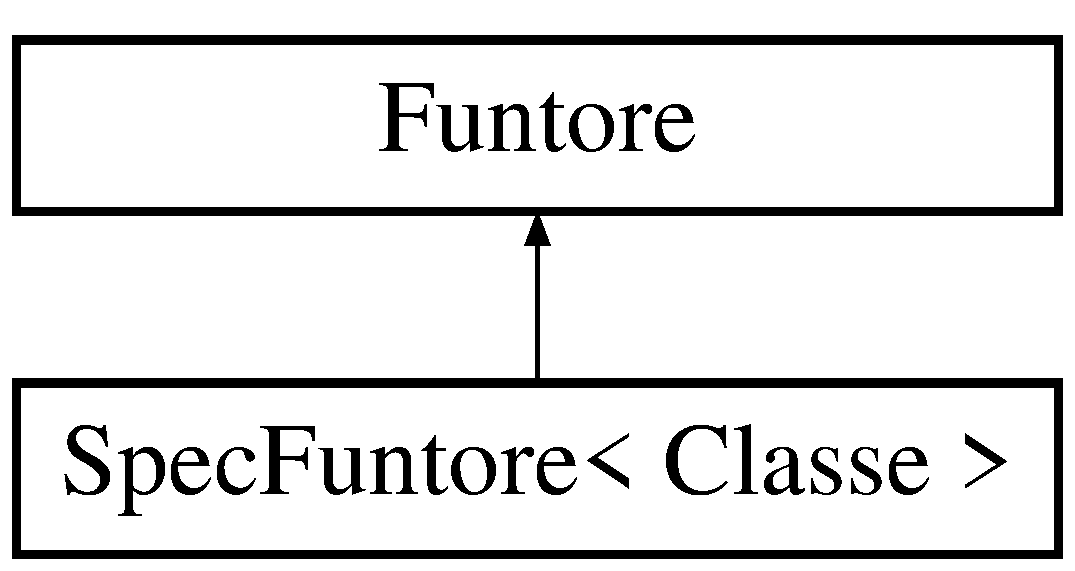
\includegraphics[height=2.000000cm]{classFuntore}
\end{center}
\end{figure}
\subsubsection*{\-Public \-Member \-Functions}
\begin{DoxyCompactItemize}
\item 
\hypertarget{classFuntore_a98ed28d91355af58355955ba885ebacb}{virtual double {\bfseries operator()} (double x)=0}\label{classFuntore_a98ed28d91355af58355955ba885ebacb}

\item 
\hypertarget{classFuntore_af020783f738a26ffbc75399721893712}{virtual double {\bfseries \-Call} (double x)=0}\label{classFuntore_af020783f738a26ffbc75399721893712}

\end{DoxyCompactItemize}


\subsubsection{\-Detailed \-Description}


\-Definition at line 340 of file \-Matematica.\-h.



\-The documentation for this class was generated from the following file\-:\begin{DoxyCompactItemize}
\item 
include/\-Matematica.\-h\end{DoxyCompactItemize}

\hypertarget{structGENERAL}{}\subsection{G\+E\+N\+E\+R\+AL Struct Reference}
\label{structGENERAL}\index{G\+E\+N\+E\+R\+AL@{G\+E\+N\+E\+R\+AL}}


General information of the system.  




{\ttfamily \#include $<$Var\+Data.\+h$>$}

\subsubsection*{Public Attributes}
\begin{DoxyCompactItemize}
\item 
double \hyperlink{structGENERAL_af51ff88ae9c6c4b9907f516c09ebf68f}{Time}\hypertarget{structGENERAL_af51ff88ae9c6c4b9907f516c09ebf68f}{}\label{structGENERAL_af51ff88ae9c6c4b9907f516c09ebf68f}

\begin{DoxyCompactList}\small\item\em Total time. \end{DoxyCompactList}\item 
double \hyperlink{structGENERAL_a30b2ceb495b99ab029b438563e5f22fa}{Temp}\hypertarget{structGENERAL_a30b2ceb495b99ab029b438563e5f22fa}{}\label{structGENERAL_a30b2ceb495b99ab029b438563e5f22fa}

\begin{DoxyCompactList}\small\item\em Temperature. \end{DoxyCompactList}\item 
double \hyperlink{structGENERAL_aded0b530ca9ce830881a607b109e709f}{Beta}\hypertarget{structGENERAL_aded0b530ca9ce830881a607b109e709f}{}\label{structGENERAL_aded0b530ca9ce830881a607b109e709f}

\begin{DoxyCompactList}\small\item\em Temperature. \end{DoxyCompactList}\item 
double \hyperlink{structGENERAL_ae35f6a776d95c5f300f4c70e2fc9bb48}{Energy} \mbox{[}3\mbox{]}\hypertarget{structGENERAL_ae35f6a776d95c5f300f4c70e2fc9bb48}{}\label{structGENERAL_ae35f6a776d95c5f300f4c70e2fc9bb48}

\begin{DoxyCompactList}\small\item\em Pot, kinetik, free. \end{DoxyCompactList}\item 
double \hyperlink{structGENERAL_a507c812f21f55c46378bfc7c30d0bc75}{Edge} \mbox{[}4\mbox{]}\hypertarget{structGENERAL_a507c812f21f55c46378bfc7c30d0bc75}{}\label{structGENERAL_a507c812f21f55c46378bfc7c30d0bc75}

\begin{DoxyCompactList}\small\item\em xyzr edges of the simulation box \end{DoxyCompactList}\item 
double \hyperlink{structGENERAL_aabbbbadc73659c7ef925b55cf4dd6aeb}{Inv\+Edge} \mbox{[}4\mbox{]}\hypertarget{structGENERAL_aabbbbadc73659c7ef925b55cf4dd6aeb}{}\label{structGENERAL_aabbbbadc73659c7ef925b55cf4dd6aeb}

\begin{DoxyCompactList}\small\item\em Inverted xyzr edges of the simulation box. \end{DoxyCompactList}\item 
double \hyperlink{structGENERAL_a7125116c90bd17b7d8d083e0e6771cb6}{Cm} \mbox{[}3\mbox{]}\hypertarget{structGENERAL_a7125116c90bd17b7d8d083e0e6771cb6}{}\label{structGENERAL_a7125116c90bd17b7d8d083e0e6771cb6}

\begin{DoxyCompactList}\small\item\em Center of mass of the system. \end{DoxyCompactList}\item 
double \hyperlink{structGENERAL_afd1b3747170c238c06ba3420cbc5c2a2}{Vel} \mbox{[}4\mbox{]}\hypertarget{structGENERAL_afd1b3747170c238c06ba3420cbc5c2a2}{}\label{structGENERAL_afd1b3747170c238c06ba3420cbc5c2a2}

\begin{DoxyCompactList}\small\item\em Velocity of the system. \end{DoxyCompactList}\item 
double \hyperlink{structGENERAL_a1c5ab9214cb52a6c7be112e52fb3a0ec}{Pre} \mbox{[}3\mbox{]}\hypertarget{structGENERAL_a1c5ab9214cb52a6c7be112e52fb3a0ec}{}\label{structGENERAL_a1c5ab9214cb52a6c7be112e52fb3a0ec}

\begin{DoxyCompactList}\small\item\em Three components of the pressure. \end{DoxyCompactList}\item 
double \hyperlink{structGENERAL_a1f1783fb13c526c8a43fac88be809a61}{v\+BB}\hypertarget{structGENERAL_a1f1783fb13c526c8a43fac88be809a61}{}\label{structGENERAL_a1f1783fb13c526c8a43fac88be809a61}

\begin{DoxyCompactList}\small\item\em Chemical potential of the water. \end{DoxyCompactList}\item 
double \hyperlink{structGENERAL_a118a5bd5025a170e18a8ec882f7292cf}{Surf\+Tens}\hypertarget{structGENERAL_a118a5bd5025a170e18a8ec882f7292cf}{}\label{structGENERAL_a118a5bd5025a170e18a8ec882f7292cf}

\begin{DoxyCompactList}\small\item\em Surface tension. \end{DoxyCompactList}\item 
double \hyperlink{structGENERAL_a1b854697afb2af2e40431c4a10c83f6a}{chiN}\hypertarget{structGENERAL_a1b854697afb2af2e40431c4a10c83f6a}{}\label{structGENERAL_a1b854697afb2af2e40431c4a10c83f6a}

\begin{DoxyCompactList}\small\item\em Incompatibility. \end{DoxyCompactList}\item 
double \hyperlink{structGENERAL_ade2b90e837653f48dc2bdb1d856dac32}{kappaN}\hypertarget{structGENERAL_ade2b90e837653f48dc2bdb1d856dac32}{}\label{structGENERAL_ade2b90e837653f48dc2bdb1d856dac32}

\begin{DoxyCompactList}\small\item\em Incompressibility. \end{DoxyCompactList}\item 
double \hyperlink{structGENERAL_a3ed57096651b587c2bf716fa78048153}{rho}\hypertarget{structGENERAL_a3ed57096651b587c2bf716fa78048153}{}\label{structGENERAL_a3ed57096651b587c2bf716fa78048153}

\begin{DoxyCompactList}\small\item\em Density coexistence. \end{DoxyCompactList}\item 
double \hyperlink{structGENERAL_a2ff77637e8d30a6568475ce5808a8b9f}{kappa\+Bend}\hypertarget{structGENERAL_a2ff77637e8d30a6568475ce5808a8b9f}{}\label{structGENERAL_a2ff77637e8d30a6568475ce5808a8b9f}

\begin{DoxyCompactList}\small\item\em Prefactor of the bending potential. \end{DoxyCompactList}\item 
double \hyperlink{structGENERAL_a907c197a31ff3bce70d5d86b03f91c02}{kappa\+Spring}\hypertarget{structGENERAL_a907c197a31ff3bce70d5d86b03f91c02}{}\label{structGENERAL_a907c197a31ff3bce70d5d86b03f91c02}

\begin{DoxyCompactList}\small\item\em Prefactor of the bond spring. \end{DoxyCompactList}\item 
double \hyperlink{structGENERAL_a6ae0a67cfc3db4a812c06c78832835ab}{Spring\+Rest}\hypertarget{structGENERAL_a6ae0a67cfc3db4a812c06c78832835ab}{}\label{structGENERAL_a6ae0a67cfc3db4a812c06c78832835ab}

\begin{DoxyCompactList}\small\item\em Rest length of the harmonic potential. \end{DoxyCompactList}\item 
double \hyperlink{structGENERAL_aa72817c7da02760c6940e2e2fcea5f02}{Re\+Over\+Cut\+Off}\hypertarget{structGENERAL_aa72817c7da02760c6940e2e2fcea5f02}{}\label{structGENERAL_aa72817c7da02760c6940e2e2fcea5f02}

\begin{DoxyCompactList}\small\item\em Convertion unit R\+\_\+e over Cut\+Off. \end{DoxyCompactList}\item 
double \hyperlink{structGENERAL_ac321dc561843cb5d3f74604036a3a8da}{Deltat}\hypertarget{structGENERAL_ac321dc561843cb5d3f74604036a3a8da}{}\label{structGENERAL_ac321dc561843cb5d3f74604036a3a8da}

\begin{DoxyCompactList}\small\item\em Timestep. \end{DoxyCompactList}\item 
double \hyperlink{structGENERAL_a3e95eddffbcb7d50ef9588ced78a148c}{W\+Func\+Straight2}\hypertarget{structGENERAL_a3e95eddffbcb7d50ef9588ced78a148c}{}\label{structGENERAL_a3e95eddffbcb7d50ef9588ced78a148c}

\begin{DoxyCompactList}\small\item\em Weighting function straight length. \end{DoxyCompactList}\item 
double \hyperlink{structGENERAL_a2db5cd020420567f6c9414964981a572}{W\+Func\+Straight3}\hypertarget{structGENERAL_a2db5cd020420567f6c9414964981a572}{}\label{structGENERAL_a2db5cd020420567f6c9414964981a572}

\begin{DoxyCompactList}\small\item\em Weighting function straight length. \end{DoxyCompactList}\item 
unsigned long \hyperlink{structGENERAL_a7d089b5d5a5a8f8699325baad0ad85b5}{Step}\hypertarget{structGENERAL_a7d089b5d5a5a8f8699325baad0ad85b5}{}\label{structGENERAL_a7d089b5d5a5a8f8699325baad0ad85b5}

\begin{DoxyCompactList}\small\item\em Courrent step. \end{DoxyCompactList}\item 
int \hyperlink{structGENERAL_abdcc792391d8c5092471dff191de47f4}{N\+Part}\hypertarget{structGENERAL_abdcc792391d8c5092471dff191de47f4}{}\label{structGENERAL_abdcc792391d8c5092471dff191de47f4}

\begin{DoxyCompactList}\small\item\em Number of particle. \end{DoxyCompactList}\item 
int \hyperlink{structGENERAL_aa49e4d7af0d71e79524ef6fb081707b5}{N\+Chain}\hypertarget{structGENERAL_aa49e4d7af0d71e79524ef6fb081707b5}{}\label{structGENERAL_aa49e4d7af0d71e79524ef6fb081707b5}

\begin{DoxyCompactList}\small\item\em Number of chain. \end{DoxyCompactList}\item 
int \hyperlink{structGENERAL_a521663d12899e0fefe0a182332a8573f}{N\+P\+Ch}\hypertarget{structGENERAL_a521663d12899e0fefe0a182332a8573f}{}\label{structGENERAL_a521663d12899e0fefe0a182332a8573f}

\begin{DoxyCompactList}\small\item\em Number of particle per chain. \end{DoxyCompactList}\item 
int \hyperlink{structGENERAL_a4c6eee002f7cf6e171979efae96f56d9}{N\+AllocP}\hypertarget{structGENERAL_a4c6eee002f7cf6e171979efae96f56d9}{}\label{structGENERAL_a4c6eee002f7cf6e171979efae96f56d9}

\begin{DoxyCompactList}\small\item\em Number of allocated particles. \end{DoxyCompactList}\item 
int \hyperlink{structGENERAL_a0d31c72beb19e7045ebd94aa02b454b5}{N\+AllocC}\hypertarget{structGENERAL_a0d31c72beb19e7045ebd94aa02b454b5}{}\label{structGENERAL_a0d31c72beb19e7045ebd94aa02b454b5}

\begin{DoxyCompactList}\small\item\em Number of allocated chains. \end{DoxyCompactList}\item 
int \hyperlink{structGENERAL_a4ad7cd0445491c0ba28c41907eba46b1}{N\+Type}\hypertarget{structGENERAL_a4ad7cd0445491c0ba28c41907eba46b1}{}\label{structGENERAL_a4ad7cd0445491c0ba28c41907eba46b1}

\begin{DoxyCompactList}\small\item\em \subsubsection*{of types of the particle}\end{DoxyCompactList}\item 
int \hyperlink{structGENERAL_a73918a2decc99bcf2317d2855dada6c8}{N\+Link}\hypertarget{structGENERAL_a73918a2decc99bcf2317d2855dada6c8}{}\label{structGENERAL_a73918a2decc99bcf2317d2855dada6c8}

\begin{DoxyCompactList}\small\item\em Maximum number of bonds. \end{DoxyCompactList}\item 
int \hyperlink{structGENERAL_a6613c7ace95c4bff9b80a9bfd8f4a9f8}{N\+Block}\hypertarget{structGENERAL_a6613c7ace95c4bff9b80a9bfd8f4a9f8}{}\label{structGENERAL_a6613c7ace95c4bff9b80a9bfd8f4a9f8}

\begin{DoxyCompactList}\small\item\em Number of blocks. \end{DoxyCompactList}\item 
int {\bfseries N\+Nano}\hypertarget{structGENERAL_a41701680890bf48215ba29ba50d61caa}{}\label{structGENERAL_a41701680890bf48215ba29ba50d61caa}

\end{DoxyCompactItemize}


\subsubsection{Detailed Description}
General information of the system. 

Definition at line 299 of file Var\+Data.\+h.



The documentation for this struct was generated from the following file\+:\begin{DoxyCompactItemize}
\item 
include/Var\+Data.\+h\end{DoxyCompactItemize}

\hypertarget{structGRIDCELL}{\subsection{\-G\-R\-I\-D\-C\-E\-L\-L \-Struct \-Reference}
\label{structGRIDCELL}\index{\-G\-R\-I\-D\-C\-E\-L\-L@{\-G\-R\-I\-D\-C\-E\-L\-L}}
}


\-All the vertex in a cell.  




{\ttfamily \#include $<$\-Var\-Data.\-h$>$}

\subsubsection*{\-Public \-Attributes}
\begin{DoxyCompactItemize}
\item 
\hypertarget{structGRIDCELL_af46bddc16e32b74aeff274ceaf5562f8}{\hyperlink{structXYZ}{\-X\-Y\-Z} \hyperlink{structGRIDCELL_af46bddc16e32b74aeff274ceaf5562f8}{p} \mbox{[}8\mbox{]}}\label{structGRIDCELL_af46bddc16e32b74aeff274ceaf5562f8}

\begin{DoxyCompactList}\small\item\em \-Vertices. \end{DoxyCompactList}\item 
\hypertarget{structGRIDCELL_a50b3da89748a7768f305af0e5a186332}{\hyperlink{structXYZ}{\-X\-Y\-Z} \hyperlink{structGRIDCELL_a50b3da89748a7768f305af0e5a186332}{n} \mbox{[}8\mbox{]}}\label{structGRIDCELL_a50b3da89748a7768f305af0e5a186332}

\begin{DoxyCompactList}\small\item\em \-Normals. \end{DoxyCompactList}\item 
\hypertarget{structGRIDCELL_a98dc06e4ef0443c670c22157e89ee97d}{double \hyperlink{structGRIDCELL_a98dc06e4ef0443c670c22157e89ee97d}{val} \mbox{[}8\mbox{]}}\label{structGRIDCELL_a98dc06e4ef0443c670c22157e89ee97d}

\begin{DoxyCompactList}\small\item\em \-Density at the vertices. \end{DoxyCompactList}\end{DoxyCompactItemize}


\subsubsection{\-Detailed \-Description}
\-All the vertex in a cell. 

\-Definition at line 489 of file \-Var\-Data.\-h.



\-The documentation for this struct was generated from the following file\-:\begin{DoxyCompactItemize}
\item 
include/\-Var\-Data.\-h\end{DoxyCompactItemize}

\hypertarget{classImpostaNBin}{\subsection{\-Imposta\-N\-Bin \-Class \-Reference}
\label{classImpostaNBin}\index{\-Imposta\-N\-Bin@{\-Imposta\-N\-Bin}}
}


\-Homemade slider.  




{\ttfamily \#include $<$\-Elementi\-Grafici.\-h$>$}

\subsubsection*{\-Public \-Slots}
\begin{DoxyCompactItemize}
\item 
\hypertarget{classImpostaNBin_a8061b6fff22eaa38700407bbf179a1ee}{void {\bfseries \-Imp\-Numero} (int)}\label{classImpostaNBin_a8061b6fff22eaa38700407bbf179a1ee}

\item 
\hypertarget{classImpostaNBin_afe52cab0e5d5fcb1ddddac6c1a10b38d}{void {\bfseries \-Imp\-Inter} (int \-Max)}\label{classImpostaNBin_afe52cab0e5d5fcb1ddddac6c1a10b38d}

\item 
\hypertarget{classImpostaNBin_a12904a8b0fbd7774c00bbcf44f6ff2f9}{void {\bfseries \-Imp\-Inter} (int \-Min, int \-Max)}\label{classImpostaNBin_a12904a8b0fbd7774c00bbcf44f6ff2f9}

\end{DoxyCompactItemize}
\subsubsection*{\-Signals}
\begin{DoxyCompactItemize}
\item 
\hypertarget{classImpostaNBin_ab1b323d7b5663b9acd07ac738d49f707}{void {\bfseries \-Valore\-Cambiato} (int)}\label{classImpostaNBin_ab1b323d7b5663b9acd07ac738d49f707}

\end{DoxyCompactItemize}
\subsubsection*{\-Public \-Member \-Functions}
\begin{DoxyCompactItemize}
\item 
\hypertarget{classImpostaNBin_a6b13f1131d1a02b8848404b52193f680}{{\bfseries \-Imposta\-N\-Bin} (\-Q\-Widget $\ast$parent, const char $\ast$name=0)}\label{classImpostaNBin_a6b13f1131d1a02b8848404b52193f680}

\item 
\hypertarget{classImpostaNBin_ad131323a76ebb0197218c09233f7359a}{void {\bfseries \-Testo} (const char $\ast$)}\label{classImpostaNBin_ad131323a76ebb0197218c09233f7359a}

\item 
\hypertarget{classImpostaNBin_ae1a67f98002156c9ae9130e248472cec}{int {\bfseries \-Numero} () const }\label{classImpostaNBin_ae1a67f98002156c9ae9130e248472cec}

\end{DoxyCompactItemize}


\subsubsection{\-Detailed \-Description}
\-Homemade slider. 

\-Definition at line 374 of file \-Elementi\-Grafici.\-h.



\-The documentation for this class was generated from the following files\-:\begin{DoxyCompactItemize}
\item 
src/\-Avvis/\-Elementi\-Grafici.\-h\item 
src/\-Avvis/\-Elementi\-Grafici.\-cpp\item 
src/\-Avvis/moc\-\_\-\-Elementi\-Grafici.\-cpp\end{DoxyCompactItemize}

\hypertarget{structKFORCES}{}\subsection{K\+F\+O\+R\+C\+ES Struct Reference}
\label{structKFORCES}\index{K\+F\+O\+R\+C\+ES@{K\+F\+O\+R\+C\+ES}}


Prefactors of the forces.  




{\ttfamily \#include $<$Forces.\+h$>$}

\subsubsection*{Public Attributes}
\begin{DoxyCompactItemize}
\item 
double \hyperlink{structKFORCES_ad68dc62d6c1b859ad3abebc60476453e}{Lap}\hypertarget{structKFORCES_ad68dc62d6c1b859ad3abebc60476453e}{}\label{structKFORCES_ad68dc62d6c1b859ad3abebc60476453e}

\begin{DoxyCompactList}\small\item\em Prefactor of the Laplacian. \end{DoxyCompactList}\item 
double \hyperlink{structKFORCES_a348745786658bd8382be1fd25066a309}{S\+Lap}\hypertarget{structKFORCES_a348745786658bd8382be1fd25066a309}{}\label{structKFORCES_a348745786658bd8382be1fd25066a309}

\begin{DoxyCompactList}\small\item\em Prefactor of the square laplacian. \end{DoxyCompactList}\item 
double \hyperlink{structKFORCES_a682d0bf554363bfcb9698c55bd6a0527}{El} \mbox{[}3\mbox{]}\hypertarget{structKFORCES_a682d0bf554363bfcb9698c55bd6a0527}{}\label{structKFORCES_a682d0bf554363bfcb9698c55bd6a0527}

\begin{DoxyCompactList}\small\item\em Elastic force. \end{DoxyCompactList}\item 
double \hyperlink{structKFORCES_a60a1f1fb24ef62e5433e4c50466a1624}{Ext}\hypertarget{structKFORCES_a60a1f1fb24ef62e5433e4c50466a1624}{}\label{structKFORCES_a60a1f1fb24ef62e5433e4c50466a1624}

\begin{DoxyCompactList}\small\item\em External force. \end{DoxyCompactList}\item 
double \hyperlink{structKFORCES_a014d64316c28b7014a2e8696ea99388f}{LJ}\hypertarget{structKFORCES_a014d64316c28b7014a2e8696ea99388f}{}\label{structKFORCES_a014d64316c28b7014a2e8696ea99388f}

\begin{DoxyCompactList}\small\item\em Lennard-\/\+Jones. \end{DoxyCompactList}\item 
double \hyperlink{structKFORCES_a426ea6ec144b001fdfc9bf8044160465}{Cont}\hypertarget{structKFORCES_a426ea6ec144b001fdfc9bf8044160465}{}\label{structKFORCES_a426ea6ec144b001fdfc9bf8044160465}

\begin{DoxyCompactList}\small\item\em Contact/\+Friction. \end{DoxyCompactList}\item 
double \hyperlink{structKFORCES_a3a05bdc0a320e2408242a0f5152debca}{Elong} \mbox{[}3\mbox{]}\hypertarget{structKFORCES_a3a05bdc0a320e2408242a0f5152debca}{}\label{structKFORCES_a3a05bdc0a320e2408242a0f5152debca}

\begin{DoxyCompactList}\small\item\em Elongation of the springs. \end{DoxyCompactList}\item 
double \hyperlink{structKFORCES_ae05456a79f8f4e14c02b374d188ba9da}{L\+J\+Min}\hypertarget{structKFORCES_ae05456a79f8f4e14c02b374d188ba9da}{}\label{structKFORCES_ae05456a79f8f4e14c02b374d188ba9da}

\begin{DoxyCompactList}\small\item\em Lennard-\/\+Jones. \end{DoxyCompactList}\item 
double \hyperlink{structKFORCES_a16102e172acd6f663f3559c3f6e7b35c}{L\+J\+Cut\+Off}\hypertarget{structKFORCES_a16102e172acd6f663f3559c3f6e7b35c}{}\label{structKFORCES_a16102e172acd6f663f3559c3f6e7b35c}

\begin{DoxyCompactList}\small\item\em Lennard-\/\+Jones. \end{DoxyCompactList}\item 
double \hyperlink{structKFORCES_ac448df5dbfd256324893075200dace49}{Cut\+Off2}\hypertarget{structKFORCES_ac448df5dbfd256324893075200dace49}{}\label{structKFORCES_ac448df5dbfd256324893075200dace49}

\begin{DoxyCompactList}\small\item\em Cut\+Off of the lennard jones. \end{DoxyCompactList}\item 
double \hyperlink{structKFORCES_a12346a80b6dd9472f0a10aab633f2f4f}{Base\+Line}\hypertarget{structKFORCES_a12346a80b6dd9472f0a10aab633f2f4f}{}\label{structKFORCES_a12346a80b6dd9472f0a10aab633f2f4f}

\begin{DoxyCompactList}\small\item\em Baseline of the potential. \end{DoxyCompactList}\item 
double \hyperlink{structKFORCES_adf3d7e8b11ee1fa9f6b7b58141ab5112}{Pot\+Thr}\hypertarget{structKFORCES_adf3d7e8b11ee1fa9f6b7b58141ab5112}{}\label{structKFORCES_adf3d7e8b11ee1fa9f6b7b58141ab5112}

\begin{DoxyCompactList}\small\item\em Maximum potential allowed. \end{DoxyCompactList}\item 
double \hyperlink{structKFORCES_ad631a0b43047f95f5bb991f5407b813e}{For\+Thr}\hypertarget{structKFORCES_ad631a0b43047f95f5bb991f5407b813e}{}\label{structKFORCES_ad631a0b43047f95f5bb991f5407b813e}

\begin{DoxyCompactList}\small\item\em Maximum force allowed. \end{DoxyCompactList}\item 
double \hyperlink{structKFORCES_a7be87fae5fde1648d34b194775515d08}{Dist\+Thr}\hypertarget{structKFORCES_a7be87fae5fde1648d34b194775515d08}{}\label{structKFORCES_a7be87fae5fde1648d34b194775515d08}

\begin{DoxyCompactList}\small\item\em Correspondent radial distance for this force. \end{DoxyCompactList}\end{DoxyCompactItemize}


\subsubsection{Detailed Description}
Prefactors of the forces. 

Definition at line 145 of file Forces.\+h.



The documentation for this struct was generated from the following file\+:\begin{DoxyCompactItemize}
\item 
src/\+Addyn/Forces.\+h\end{DoxyCompactItemize}

\hypertarget{structLINKS}{\subsection{\-L\-I\-N\-K\-S \-Struct \-Reference}
\label{structLINKS}\index{\-L\-I\-N\-K\-S@{\-L\-I\-N\-K\-S}}
}


\-Structure with the links of the particles.  




{\ttfamily \#include $<$\-Var\-Data.\-h$>$}

\subsubsection*{\-Public \-Attributes}
\begin{DoxyCompactItemize}
\item 
\hypertarget{structLINKS_aefc83dee460fda66ca240e011e7ce0a7}{int $\ast$ \hyperlink{structLINKS_aefc83dee460fda66ca240e011e7ce0a7}{\-Link}}\label{structLINKS_aefc83dee460fda66ca240e011e7ce0a7}

\begin{DoxyCompactList}\small\item\em with whom is bonded \end{DoxyCompactList}\item 
\hypertarget{structLINKS_a73918a2decc99bcf2317d2855dada6c8}{int \hyperlink{structLINKS_a73918a2decc99bcf2317d2855dada6c8}{\-N\-Link}}\label{structLINKS_a73918a2decc99bcf2317d2855dada6c8}

\begin{DoxyCompactList}\small\item\em \-How many links per particle. \end{DoxyCompactList}\end{DoxyCompactItemize}


\subsubsection{\-Detailed \-Description}
\-Structure with the links of the particles. 

\-Definition at line 229 of file \-Var\-Data.\-h.



\-The documentation for this struct was generated from the following file\-:\begin{DoxyCompactItemize}
\item 
include/\-Var\-Data.\-h\end{DoxyCompactItemize}

\hypertarget{classMatematica}{\subsection{\-Matematica \-Class \-Reference}
\label{classMatematica}\index{\-Matematica@{\-Matematica}}
}


\-Implementation of useful algorythms.  




{\ttfamily \#include $<$\-Matematica.\-h$>$}

\-Inheritance diagram for \-Matematica\-:\begin{figure}[H]
\begin{center}
\leavevmode
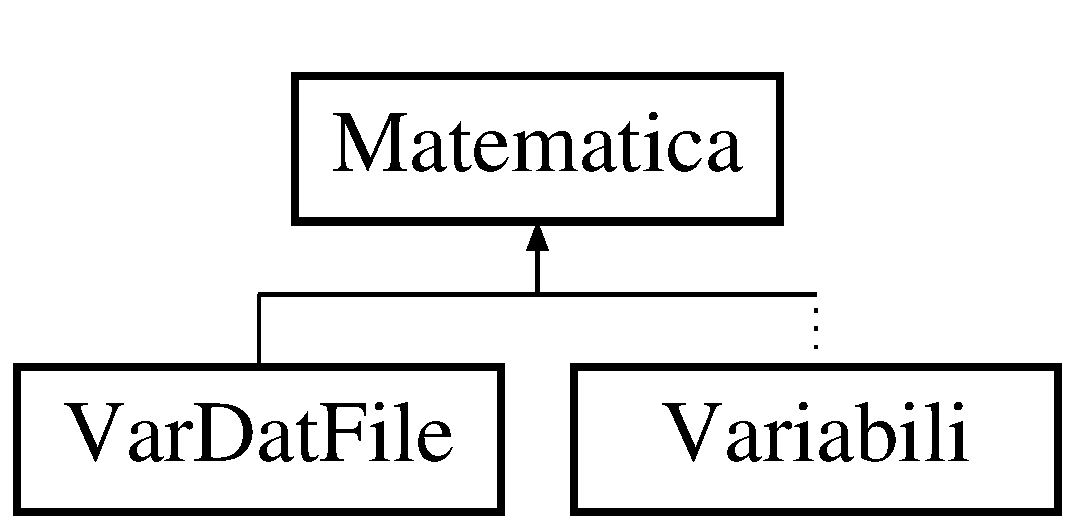
\includegraphics[height=2.000000cm]{classMatematica}
\end{center}
\end{figure}
\subsubsection*{\-Public \-Types}
\begin{DoxyCompactItemize}
\item 
\hypertarget{classMatematica_af3e0600f7cea754ca1ebefb85de3526b}{typedef double(\-Matematica\-::$\ast$ \hyperlink{classMatematica_af3e0600f7cea754ca1ebefb85de3526b}{\-F\-U\-N\-C} )(double x)}\label{classMatematica_af3e0600f7cea754ca1ebefb85de3526b}

\begin{DoxyCompactList}\small\item\em \-A tipical f(x) function. \end{DoxyCompactList}\item 
\hypertarget{classMatematica_a71f04c72c044751a72c3e605301a8b9d}{typedef void(\-Matematica\-::$\ast$ {\bfseries \-E\-L\-A\-B} )(double $\ast$st, double $\ast$sw, int \-N\-Mass)}\label{classMatematica_a71f04c72c044751a72c3e605301a8b9d}

\end{DoxyCompactItemize}
\subsubsection*{\-Public \-Member \-Functions}
\begin{DoxyCompactItemize}
\item 
\hypertarget{classMatematica_ad7fef8b66845538830977c8db143e9ae}{\hyperlink{classMatematica_ad7fef8b66845538830977c8db143e9ae}{\-Matematica} ()}\label{classMatematica_ad7fef8b66845538830977c8db143e9ae}

\begin{DoxyCompactList}\small\item\em \-Constructor. \end{DoxyCompactList}\item 
\hypertarget{classMatematica_ab5122ddcd9bce12ff5049a5ad2b5cb6d}{int \hyperlink{classMatematica_ab5122ddcd9bce12ff5049a5ad2b5cb6d}{\-Permute\-Random\-All} (int $\ast$\-Sequence, int \-N\-Mass)}\label{classMatematica_ab5122ddcd9bce12ff5049a5ad2b5cb6d}

\begin{DoxyCompactList}\small\item\em \-Permutes a sequence without repeating. \end{DoxyCompactList}\item 
\hypertarget{classMatematica_a5ee47a0f414d52f4d97c5266677cc952}{int \hyperlink{classMatematica_a5ee47a0f414d52f4d97c5266677cc952}{\-Permute\-Random\-All} (\hyperlink{structPERMUTE}{\-P\-E\-R\-M\-U\-T\-E} $\ast$\-Sequence, int \-N\-Mass)}\label{classMatematica_a5ee47a0f414d52f4d97c5266677cc952}

\begin{DoxyCompactList}\small\item\em \-Permutes a sequence without repeating. \end{DoxyCompactList}\item 
int \hyperlink{classMatematica_a486baea1c22d2accfe267ef415b3abaf}{\-Apply\-Filter} (\hyperlink{classMatrice}{\-Matrice} $\ast$\-Point, \hyperlink{classMatrice}{\-Matrice} $\ast$\-Res, \hyperlink{classMatrice}{\-Matrice} $\ast$\-Mask)
\begin{DoxyCompactList}\small\item\em \-Applies the filter. \end{DoxyCompactList}\item 
int \hyperlink{classMatematica_a4b258fe1b33ec22774aa535d1390c746}{\-Apply\-Filter} (\hyperlink{classMatrice}{\-Matrice} $\ast$\-Res, \hyperlink{classMatrice}{\-Matrice} $\ast$\-Mask)
\begin{DoxyCompactList}\small\item\em \-Applies the filter. \end{DoxyCompactList}\item 
\hypertarget{classMatematica_a3c54bdff136c7c0107e035f80232c00f}{int \hyperlink{classMatematica_a3c54bdff136c7c0107e035f80232c00f}{\-Transform} (int $\ast$\-Out, int $\ast$\-In, int \-N\-Edge, int operation)}\label{classMatematica_a3c54bdff136c7c0107e035f80232c00f}

\begin{DoxyCompactList}\small\item\em \-Boh. \end{DoxyCompactList}\item 
\hypertarget{classMatematica_abfaf13060e1740268d65e5a38a410cd6}{void \hyperlink{classMatematica_abfaf13060e1740268d65e5a38a410cd6}{\-Back\-Fold} (\hyperlink{classMatrice}{\-Matrice} $\ast$\-In, \hyperlink{classMatrice}{\-Matrice} $\ast$\-Out, int \-N\-Shift)}\label{classMatematica_abfaf13060e1740268d65e5a38a410cd6}

\begin{DoxyCompactList}\small\item\em \-Shift all the rows upwards/downwards. \end{DoxyCompactList}\item 
\hypertarget{classMatematica_a2cd25ce574ac8496d0228106f1acb7e6}{void \hyperlink{classMatematica_a2cd25ce574ac8496d0228106f1acb7e6}{\-Smooth} (double $\ast$st, double $\ast$sw, int \-N\-In, int \-N\-Out)}\label{classMatematica_a2cd25ce574ac8496d0228106f1acb7e6}

\begin{DoxyCompactList}\small\item\em \-Smooth the line with \-B\-Splines. \end{DoxyCompactList}\item 
\hypertarget{classMatematica_a628ac1d3c644d78362e0ec3aff1d2448}{double \hyperlink{classMatematica_a628ac1d3c644d78362e0ec3aff1d2448}{\-Evalx} (double x)}\label{classMatematica_a628ac1d3c644d78362e0ec3aff1d2448}

\begin{DoxyCompactList}\small\item\em \-Pointer to a generic function. \end{DoxyCompactList}\item 
\hypertarget{classMatematica_a2dd3ba2334c4444c4ef406347618c170}{double \hyperlink{classMatematica_a2dd3ba2334c4444c4ef406347618c170}{\-Contact\-Angle} (double x)}\label{classMatematica_a2dd3ba2334c4444c4ef406347618c170}

\begin{DoxyCompactList}\small\item\em \-Definition of the contact angle. \end{DoxyCompactList}\item 
\hypertarget{classMatematica_a4f67dd8ca48e4eccf15e32c736db6621}{double \hyperlink{classMatematica_a4f67dd8ca48e4eccf15e32c736db6621}{f\-Prova} (double x)}\label{classMatematica_a4f67dd8ca48e4eccf15e32c736db6621}

\begin{DoxyCompactList}\small\item\em \-Trial function. \end{DoxyCompactList}\item 
\hypertarget{classMatematica_a033b6eb7c18cac84239173ca4f210fed}{double \hyperlink{classMatematica_a033b6eb7c18cac84239173ca4f210fed}{\-F} (double \-T\-D, double \-T)}\label{classMatematica_a033b6eb7c18cac84239173ca4f210fed}

\begin{DoxyCompactList}\small\item\em \-Boh. \end{DoxyCompactList}\item 
\hypertarget{classMatematica_ad572ab06bc7d7c29e3f1043541f69da8}{double \hyperlink{classMatematica_ad572ab06bc7d7c29e3f1043541f69da8}{\-Df} (double x, double \-Delta)}\label{classMatematica_ad572ab06bc7d7c29e3f1043541f69da8}

\begin{DoxyCompactList}\small\item\em \-Boh. \end{DoxyCompactList}\item 
void \hyperlink{classMatematica_aef286a585b6e7d30107ba8f36032e3ad}{\-Elab\-St} (double $\ast$st, double $\ast$sw, int \-N\-Mass)
\begin{DoxyCompactList}\small\item\em \-Pointer to a function which operates on. \end{DoxyCompactList}\item 
void \hyperlink{classMatematica_a6393bbfadafe6c13c2e94b79c7764d4b}{\-Derivata} (double $\ast$st, double $\ast$sw, int \-N\-Mass)
\begin{DoxyCompactList}\small\item\em \-Derivate of. \end{DoxyCompactList}\item 
void \hyperlink{classMatematica_a0ffa5ec4ebf021c7e8b2e79bed9524e1}{\-Der\-O4} (double $\ast$st, double $\ast$sw, int \-N\-Mass)
\begin{DoxyCompactList}\small\item\em \-Derivate \-O(4) of. \end{DoxyCompactList}\item 
double \hyperlink{classMatematica_a7f6e9a0a72348c10d08e388e75978d25}{\-Integrazione} (double $\ast$\-Punti, double $\ast$sw, int \-N\-Mass)
\begin{DoxyCompactList}\small\item\em \-Integral of. \end{DoxyCompactList}\item 
\hypertarget{classMatematica_aa6998b41af5fad626bb70cc6fac6410e}{void \hyperlink{classMatematica_aa6998b41af5fad626bb70cc6fac6410e}{\-Integra\-A3} ()}\label{classMatematica_aa6998b41af5fad626bb70cc6fac6410e}

\begin{DoxyCompactList}\small\item\em \-Perform a integration of a \-L\-J6 \-Potential. \end{DoxyCompactList}\item 
\hypertarget{classMatematica_a150471024129f85823beffb064c4df19}{void \hyperlink{classMatematica_a150471024129f85823beffb064c4df19}{\-Square\-Gradient} (double $\ast$st, double $\ast$sw, int \-N\-Mass)}\label{classMatematica_a150471024129f85823beffb064c4df19}

\begin{DoxyCompactList}\small\item\em \-Square of the gradient. \end{DoxyCompactList}\item 
double \hyperlink{classMatematica_ac1a876ecf4d7f14cc38a7add8f6ba984}{\-Integrazione} (double a, double b)
\begin{DoxyCompactList}\small\item\em \-Integrates the function within. \end{DoxyCompactList}\item 
\hypertarget{classMatematica_a5382dfb3aa67420d9fbd6619c1aa7796}{double \hyperlink{classMatematica_a5382dfb3aa67420d9fbd6619c1aa7796}{\-Integrazione\-Gauss} (double a, double b, double \-Scarto)}\label{classMatematica_a5382dfb3aa67420d9fbd6619c1aa7796}

\begin{DoxyCompactList}\small\item\em \-Itegrate a \-Gaussian. \end{DoxyCompactList}\item 
int \hyperlink{classMatematica_af1e1e5332753626f39db69dca411ecfc}{\-Zeri} (double a, double b, double $\ast$\-Radici, int \-N\-Radici)
\begin{DoxyCompactList}\small\item\em \-Find the. \end{DoxyCompactList}\item 
\hypertarget{classMatematica_a5b8fbf8c761f9756710aeed5caed4c5e}{\hyperlink{structRADICE}{\-R\-A\-D\-I\-C\-E} \hyperlink{classMatematica_a5b8fbf8c761f9756710aeed5caed4c5e}{\-Regula\-Falsi} (double a, double b)}\label{classMatematica_a5b8fbf8c761f9756710aeed5caed4c5e}

\begin{DoxyCompactList}\small\item\em \-Use regula falsi algorithm to find the roots. \end{DoxyCompactList}\item 
\hypertarget{classMatematica_a721bd6eae0ff0aa70b8b37327b084e78}{\hyperlink{structRADICE}{\-R\-A\-D\-I\-C\-E} \hyperlink{classMatematica_a721bd6eae0ff0aa70b8b37327b084e78}{\-Newton} (double a)}\label{classMatematica_a721bd6eae0ff0aa70b8b37327b084e78}

\begin{DoxyCompactList}\small\item\em \-Use \-Newton to find the roots. \end{DoxyCompactList}\item 
\hypertarget{classMatematica_a72c0cbce789095808b5c49d3f7f8fee8}{double \hyperlink{classMatematica_a72c0cbce789095808b5c49d3f7f8fee8}{\-Estremo} (double a, double b)}\label{classMatematica_a72c0cbce789095808b5c49d3f7f8fee8}

\begin{DoxyCompactList}\small\item\em \-Other algorithm to find the roots. \end{DoxyCompactList}\item 
\hypertarget{classMatematica_a28deb4e354f861587181caac4a5b9857}{double \hyperlink{classMatematica_a28deb4e354f861587181caac4a5b9857}{\-Fattoriale} (int n)}\label{classMatematica_a28deb4e354f861587181caac4a5b9857}

\begin{DoxyCompactList}\small\item\em \-Compute the factorial. \end{DoxyCompactList}\item 
\hypertarget{classMatematica_a0a9c482dfadf895f3b52888b33121c43}{double \hyperlink{classMatematica_a0a9c482dfadf895f3b52888b33121c43}{\-Gamma} (int n)}\label{classMatematica_a0a9c482dfadf895f3b52888b33121c43}

\begin{DoxyCompactList}\small\item\em \-Euler's gamma. \end{DoxyCompactList}\item 
\hypertarget{classMatematica_a81f44d652f61225a2725c0cb3cbc9524}{double \hyperlink{classMatematica_a81f44d652f61225a2725c0cb3cbc9524}{\-Elevato} (double x, int \-Volte)}\label{classMatematica_a81f44d652f61225a2725c0cb3cbc9524}

\begin{DoxyCompactList}\small\item\em \-Integer power. \end{DoxyCompactList}\item 
\hypertarget{classMatematica_af0a86b99b1cdbff64505cdef059e6d15}{double \hyperlink{classMatematica_af0a86b99b1cdbff64505cdef059e6d15}{\-Bessel} (double \-Val, int \-Ord)}\label{classMatematica_af0a86b99b1cdbff64505cdef059e6d15}

\begin{DoxyCompactList}\small\item\em \-Bessel function. \end{DoxyCompactList}\item 
\hypertarget{classMatematica_a9dce8aab3f083e3071a47fa4d2b1b582}{double \hyperlink{classMatematica_a9dce8aab3f083e3071a47fa4d2b1b582}{\-Neumann} (double \-Val, int \-Ord)}\label{classMatematica_a9dce8aab3f083e3071a47fa4d2b1b582}

\begin{DoxyCompactList}\small\item\em \-Neumann function. \end{DoxyCompactList}\item 
\hypertarget{classMatematica_a3ea54c21e1dfc6cb0108483eca97f7cd}{double \hyperlink{classMatematica_a3ea54c21e1dfc6cb0108483eca97f7cd}{\-Segno} (int n)}\label{classMatematica_a3ea54c21e1dfc6cb0108483eca97f7cd}

\begin{DoxyCompactList}\small\item\em \-Sign of -\/$^\wedge$n. \end{DoxyCompactList}\item 
\hypertarget{classMatematica_af5ab240211f6f0aeada6022a32585acb}{double \hyperlink{classMatematica_af5ab240211f6f0aeada6022a32585acb}{\-Quasi\-Bessel} (double \-Val, int \-Ord)}\label{classMatematica_af5ab240211f6f0aeada6022a32585acb}

\begin{DoxyCompactList}\small\item\em \-A faster \-Bessel. \end{DoxyCompactList}\item 
\hypertarget{classMatematica_abee4e33f52ba1babbe9d2422e835ece5}{double \hyperlink{classMatematica_abee4e33f52ba1babbe9d2422e835ece5}{\-Quasi\-Neumann} (double \-Val, int \-Ord)}\label{classMatematica_abee4e33f52ba1babbe9d2422e835ece5}

\begin{DoxyCompactList}\small\item\em \-A faster \-Neumann. \end{DoxyCompactList}\item 
\hypertarget{classMatematica_a8ffbe3b65717720f6a91536c9be08c12}{double \hyperlink{classMatematica_a8ffbe3b65717720f6a91536c9be08c12}{\-Weight\-Function} (double x, double a)}\label{classMatematica_a8ffbe3b65717720f6a91536c9be08c12}

\begin{DoxyCompactList}\small\item\em \-Definition of a weighting function. \end{DoxyCompactList}\item 
\hypertarget{classMatematica_a3381e7982dc433288e7ddac251a8e995}{double \hyperlink{classMatematica_a3381e7982dc433288e7ddac251a8e995}{\-Weight\-Function2} (double x, double a)}\label{classMatematica_a3381e7982dc433288e7ddac251a8e995}

\begin{DoxyCompactList}\small\item\em \-Definition of a weighting function. \end{DoxyCompactList}\item 
\hypertarget{classMatematica_aac48860fd7ddec8063e83f2a401d964e}{double \hyperlink{classMatematica_aac48860fd7ddec8063e83f2a401d964e}{\-L\-J\-Hamaker} (double r, double r\-\_\-np, double theta)}\label{classMatematica_aac48860fd7ddec8063e83f2a401d964e}

\begin{DoxyCompactList}\small\item\em \-Integration of the \-L\-J 6 term. \end{DoxyCompactList}\item 
\hypertarget{classMatematica_a51d698727558e19853a9b5b57d408cce}{double \hyperlink{classMatematica_a51d698727558e19853a9b5b57d408cce}{\-L\-J\-Hamaker\-Cum} (double \-Rad, double \-Rad\-Np\-Min, double \-Rad\-Np\-Max)}\label{classMatematica_a51d698727558e19853a9b5b57d408cce}

\begin{DoxyCompactList}\small\item\em \-Integrate over r\-\_\-np up to \-Rad\-Np. \end{DoxyCompactList}\item 
\hypertarget{classMatematica_a1a96fd9eb322682d6239edae5786df00}{double \hyperlink{classMatematica_a1a96fd9eb322682d6239edae5786df00}{\-L\-J\-Hamaker} (double \-Rad, double r\-\_\-np)}\label{classMatematica_a1a96fd9eb322682d6239edae5786df00}

\begin{DoxyCompactList}\small\item\em \-Integrate over theta. \end{DoxyCompactList}\item 
\hypertarget{classMatematica_a1dad46d7d3646dfe812d20dd22e06513}{double \hyperlink{classMatematica_a1dad46d7d3646dfe812d20dd22e06513}{\-L\-J39} (double r, double r\-\_\-np)}\label{classMatematica_a1dad46d7d3646dfe812d20dd22e06513}

\begin{DoxyCompactList}\small\item\em \-Integration of the \-L\-J 6 term. \end{DoxyCompactList}\item 
\hypertarget{classMatematica_ad9ec0b6378fe8077c460449a16404ca7}{void \hyperlink{classMatematica_ad9ec0b6378fe8077c460449a16404ca7}{\-Exec\-Command} (double $\ast$st, double $\ast$st1, int \-N\-Mass, char $\ast$cmd)}\label{classMatematica_ad9ec0b6378fe8077c460449a16404ca7}

\begin{DoxyCompactList}\small\item\em \-Execute a command defined in string. \end{DoxyCompactList}\item 
\hypertarget{classMatematica_aa8b3417ffb15a1c67df01163d9d2fc35}{double \hyperlink{classMatematica_aa8b3417ffb15a1c67df01163d9d2fc35}{\-Exec\-Formula} (double x, double y, char $\ast$cmd)}\label{classMatematica_aa8b3417ffb15a1c67df01163d9d2fc35}

\begin{DoxyCompactList}\small\item\em \-Execute a formula. \end{DoxyCompactList}\item 
\hypertarget{classMatematica_a2d18b53fcf726b2a08d6c737033bde80}{double \hyperlink{classMatematica_a2d18b53fcf726b2a08d6c737033bde80}{\-Exec\-Formula} (double $\ast$$\ast$st, int n, char $\ast$cmd)}\label{classMatematica_a2d18b53fcf726b2a08d6c737033bde80}

\begin{DoxyCompactList}\small\item\em \-Execute a formula. \end{DoxyCompactList}\item 
\hypertarget{classMatematica_a21b0d93a1241a634ee8719c941619e4b}{double \hyperlink{classMatematica_a21b0d93a1241a634ee8719c941619e4b}{\-Gauss} (double \-Media, double \-Scarto, double x)}\label{classMatematica_a21b0d93a1241a634ee8719c941619e4b}

\begin{DoxyCompactList}\small\item\em \-Gaussian. \end{DoxyCompactList}\item 
\hypertarget{classMatematica_af622f5a2f12722fd5ed7f8840fa730bd}{bool \hyperlink{classMatematica_af622f5a2f12722fd5ed7f8840fa730bd}{\-Inizializza\-Gaussiano} (double \-Scarto, int \-N)}\label{classMatematica_af622f5a2f12722fd5ed7f8840fa730bd}

\begin{DoxyCompactList}\small\item\em \-Initialize the \-Gaussian number generator. \end{DoxyCompactList}\item 
double \hyperlink{classMatematica_ad14013038c5963ed49ca1236e681db10}{\-Gaussiano} (double \-Media, double \-Scarto)
\begin{DoxyCompactList}\small\item\em \-Gaussian random number. \end{DoxyCompactList}\item 
\hypertarget{classMatematica_abe4888052d3a0b30d84f2b4c7a523328}{void \hyperlink{classMatematica_abe4888052d3a0b30d84f2b4c7a523328}{\-Spettro} (double $\ast$st, double $\ast$sw, int \-N\-Mass)}\label{classMatematica_abe4888052d3a0b30d84f2b4c7a523328}

\begin{DoxyCompactList}\small\item\em \-Compute the spectrum. \end{DoxyCompactList}\item 
void \hyperlink{classMatematica_a817fad189f184396efc334a2429fdf7a}{\-Spettro2d} (double $\ast$st, double $\ast$sw, int \-N\-Mass)
\begin{DoxyCompactList}\small\item\em \-Compute the 2d spectrum of. \end{DoxyCompactList}\item 
void \hyperlink{classMatematica_a4529a3aade5c9592905c7febebac662a}{\-Spettro2d} (double $\ast$st, double $\ast$$\ast$sw, int \-N\-Mass)
\begin{DoxyCompactList}\small\item\em \-Compute the 2d spectrum of. \end{DoxyCompactList}\item 
\hypertarget{classMatematica_a8244ce9b83c8b38d0004086377ec137c}{void \hyperlink{classMatematica_a8244ce9b83c8b38d0004086377ec137c}{\-Spettro\-D\-F\-T} (double $\ast$st, double $\ast$sw, int \-N\-Mass)}\label{classMatematica_a8244ce9b83c8b38d0004086377ec137c}

\begin{DoxyCompactList}\small\item\em \-D\-F\-T implementation of the spectrum, slow. \end{DoxyCompactList}\item 
\hypertarget{classMatematica_aeac3632a9ced53cee7f0bda92208dd07}{void \hyperlink{classMatematica_aeac3632a9ced53cee7f0bda92208dd07}{\-Radice} (double $\ast$st, double $\ast$sw, int \-N)}\label{classMatematica_aeac3632a9ced53cee7f0bda92208dd07}

\begin{DoxyCompactList}\small\item\em \-Compute the root of the signal. \end{DoxyCompactList}\item 
\hypertarget{classMatematica_a6410e1f3b747f1e313e9d3bcffe004ce}{void \hyperlink{classMatematica_a6410e1f3b747f1e313e9d3bcffe004ce}{\-Autocor} (bool $\ast$st, double $\ast$s\-Auto, int \-N)}\label{classMatematica_a6410e1f3b747f1e313e9d3bcffe004ce}

\begin{DoxyCompactList}\small\item\em \-Compute the autocorrelation of a boolean signal. \end{DoxyCompactList}\item 
\hypertarget{classMatematica_af0661121d63e1dddda156d2e46b4c39d}{void \hyperlink{classMatematica_af0661121d63e1dddda156d2e46b4c39d}{\-Autocor} (double $\ast$st, double $\ast$s\-Auto, int \-N\-Mass)}\label{classMatematica_af0661121d63e1dddda156d2e46b4c39d}

\begin{DoxyCompactList}\small\item\em \-Compute the autocorrelation of the signal. \end{DoxyCompactList}\item 
\hypertarget{classMatematica_a842d80157ade9075dce41b8b9f4bb4f3}{double \hyperlink{classMatematica_a842d80157ade9075dce41b8b9f4bb4f3}{\-Norm} (double $\ast$st, int \-N\-Mass)}\label{classMatematica_a842d80157ade9075dce41b8b9f4bb4f3}

\begin{DoxyCompactList}\small\item\em \-Norm of an array. \end{DoxyCompactList}\item 
\hypertarget{classMatematica_ac3425ea4b3f1bc9999c7b6442b106ebe}{int \hyperlink{classMatematica_ac3425ea4b3f1bc9999c7b6442b106ebe}{\-Normalize\-Area} (double $\ast$st, int \-N\-Mass)}\label{classMatematica_ac3425ea4b3f1bc9999c7b6442b106ebe}

\begin{DoxyCompactList}\small\item\em \-Normalize. \end{DoxyCompactList}\item 
\hypertarget{classMatematica_a30066e752b4f5504770d8d8c5687972a}{void \hyperlink{classMatematica_a30066e752b4f5504770d8d8c5687972a}{\-Normalize\-Vect} (double $\ast$st, int \-N\-Mass)}\label{classMatematica_a30066e752b4f5504770d8d8c5687972a}

\begin{DoxyCompactList}\small\item\em \-Normalize. \end{DoxyCompactList}\item 
\hypertarget{classMatematica_aa51fbe747c2dcd8d72980b9624be93a1}{int \hyperlink{classMatematica_aa51fbe747c2dcd8d72980b9624be93a1}{\-Normalizza} (double $\ast$st, int \-N\-Mass)}\label{classMatematica_aa51fbe747c2dcd8d72980b9624be93a1}

\begin{DoxyCompactList}\small\item\em \-Normalize. \end{DoxyCompactList}\item 
\hypertarget{classMatematica_a3221d7079785ecb693e84532d784c302}{int \hyperlink{classMatematica_a3221d7079785ecb693e84532d784c302}{\-Normalizza} (double $\ast$st, double $\ast$sw, int \-N\-Mass)}\label{classMatematica_a3221d7079785ecb693e84532d784c302}

\begin{DoxyCompactList}\small\item\em \-Normalize. \end{DoxyCompactList}\item 
\hypertarget{classMatematica_a4e641eb6229cee6b8fb5674433fc2da5}{void \hyperlink{classMatematica_a4e641eb6229cee6b8fb5674433fc2da5}{\-Modulo} (double $\ast$st, double $\ast$sw, int \-N\-Mass)}\label{classMatematica_a4e641eb6229cee6b8fb5674433fc2da5}

\begin{DoxyCompactList}\small\item\em \-Compute the modulus. \end{DoxyCompactList}\item 
\hypertarget{classMatematica_a99d5aa828752a12f2c5bc2033e00d0ad}{void \hyperlink{classMatematica_a99d5aa828752a12f2c5bc2033e00d0ad}{\-Media\-Mobile} (double $\ast$st, int \-N\-Mass, double $\ast$sw, int \-Parti)}\label{classMatematica_a99d5aa828752a12f2c5bc2033e00d0ad}

\begin{DoxyCompactList}\small\item\em \-Running average. \end{DoxyCompactList}\item 
\hypertarget{classMatematica_a0529a1c2450d94429ff81273ce35cd42}{int \hyperlink{classMatematica_a0529a1c2450d94429ff81273ce35cd42}{\-Media\-Mobile} (double $\ast$st, int \-N\-Mass, double $\ast$sw, double $\ast$s\-Err, int \-Parti)}\label{classMatematica_a0529a1c2450d94429ff81273ce35cd42}

\begin{DoxyCompactList}\small\item\em \-Running average. \end{DoxyCompactList}\item 
\hypertarget{classMatematica_acc472956dae6f7628bad8d4ca7f7ed68}{int \hyperlink{classMatematica_acc472956dae6f7628bad8d4ca7f7ed68}{\-Correla\-Due\-Punti} (double $\ast$st, int \-N\-Mass, double $\ast$sw, int \-Punti)}\label{classMatematica_acc472956dae6f7628bad8d4ca7f7ed68}

\begin{DoxyCompactList}\small\item\em \-Two points correlation. \end{DoxyCompactList}\item 
\hypertarget{classMatematica_ac6fad3beb60e7a8d3b35e40a1eb98fb3}{void \hyperlink{classMatematica_ac6fad3beb60e7a8d3b35e40a1eb98fb3}{\-Autosimilarita} (double $\ast$st, int \-N\-Mass, double $\ast$sw, int \-Valori)}\label{classMatematica_ac6fad3beb60e7a8d3b35e40a1eb98fb3}

\begin{DoxyCompactList}\small\item\em \-Self similarity. \end{DoxyCompactList}\item 
\hypertarget{classMatematica_a39b05b88f4b8ec478bd4da89c0e469d0}{\hyperlink{structMOMENTI}{\-M\-O\-M\-E\-N\-T\-I} \hyperlink{classMatematica_a39b05b88f4b8ec478bd4da89c0e469d0}{\-Distribuzione} (const double $\ast$st, int \-N\-Mass)}\label{classMatematica_a39b05b88f4b8ec478bd4da89c0e469d0}

\begin{DoxyCompactList}\small\item\em \-Moments of a signal. \end{DoxyCompactList}\item 
\hypertarget{classMatematica_a1ab633f13d7ee483931d6b17f9fb0164}{\hyperlink{structMOMENTI}{\-M\-O\-M\-E\-N\-T\-I} \hyperlink{classMatematica_a1ab633f13d7ee483931d6b17f9fb0164}{\-Distribuzione} (const double $\ast$st, int \-N\-Mass, double $\ast$\-Intervalli, int \-Valori, int \-If\-Norm)}\label{classMatematica_a1ab633f13d7ee483931d6b17f9fb0164}

\begin{DoxyCompactList}\small\item\em \-Moments and histogram of a signal. \end{DoxyCompactList}\item 
\hypertarget{classMatematica_a45b9e8e40b9d8107cbfdb92cec130ea3}{\hyperlink{structMOMENTI}{\-M\-O\-M\-E\-N\-T\-I} \hyperlink{classMatematica_a45b9e8e40b9d8107cbfdb92cec130ea3}{\-Distribuzione} (const double $\ast$st, int \-N\-Mass, double $\ast$\-Intervalli, int \-Valori, double $\ast$\-Confine, int \-If\-Norm)}\label{classMatematica_a45b9e8e40b9d8107cbfdb92cec130ea3}

\begin{DoxyCompactList}\small\item\em \-Moments and histogram of a signal between two values. \end{DoxyCompactList}\item 
\hypertarget{classMatematica_a5e8fb8fff251f8594af3f6ec809bdd46}{\hyperlink{structMOMENTI}{\-M\-O\-M\-E\-N\-T\-I} \hyperlink{classMatematica_a5e8fb8fff251f8594af3f6ec809bdd46}{\-Distr\-Err} (const double $\ast$st, int \-N\-Mass, double $\ast$\-Intervalli, double $\ast$\-Err, int \-Valori, double $\ast$\-Confine, int \-If\-Norm)}\label{classMatematica_a5e8fb8fff251f8594af3f6ec809bdd46}

\begin{DoxyCompactList}\small\item\em \-Moments and histogram of a signal between two values. \end{DoxyCompactList}\item 
\hypertarget{classMatematica_a558ecd17e8fec096693541f1d83545ae}{\hyperlink{structMOMENTI}{\-M\-O\-M\-E\-N\-T\-I} \hyperlink{classMatematica_a558ecd17e8fec096693541f1d83545ae}{\-Distribuzione\-Gauss} (const double $\ast$st, int \-N\-Mass, double $\ast$\-Intervalli, double $\ast$d\-Int, int \-Valori, int \-If\-Norm)}\label{classMatematica_a558ecd17e8fec096693541f1d83545ae}

\begin{DoxyCompactList}\small\item\em \-Look for the \-Gaussian distribution. \end{DoxyCompactList}\item 
\hypertarget{classMatematica_afbd5fb94779d51392400156cd2210035}{\hyperlink{structMOMENTI}{\-M\-O\-M\-E\-N\-T\-I} \hyperlink{classMatematica_afbd5fb94779d51392400156cd2210035}{\-Distribuzione\-Maxwell} (const double $\ast$st, int \-N\-Mass, double $\ast$\-Intervalli, double $\ast$d\-Int, int \-Valori, int \-If\-Norm)}\label{classMatematica_afbd5fb94779d51392400156cd2210035}

\begin{DoxyCompactList}\small\item\em \-Look for the \-Maxwellian distribution. \end{DoxyCompactList}\item 
\hypertarget{classMatematica_ab160279d67e4266427d7de4983249bd4}{void \hyperlink{classMatematica_ab160279d67e4266427d7de4983249bd4}{\-Distr\-Sample} (double $\ast$\-Px, double $\ast$\-Py, int \-N\-Max, double $\ast$$\ast$\-Distr, int \-N\-Bin, const int \-N\-Sample, int \-If\-Norm, double $\ast$x\-Bound)}\label{classMatematica_ab160279d67e4266427d7de4983249bd4}

\begin{DoxyCompactList}\small\item\em \-Compare the distribution of a sample of data. \end{DoxyCompactList}\item 
\hypertarget{classMatematica_a54768724636e1877a0f515037f9c1dfd}{\hyperlink{structMOMENTI}{\-M\-O\-M\-E\-N\-T\-I} \hyperlink{classMatematica_a54768724636e1877a0f515037f9c1dfd}{\-Weight\-Average} (const double $\ast$sx, const double $\ast$sy, int \-N\-Max)}\label{classMatematica_a54768724636e1877a0f515037f9c1dfd}

\begin{DoxyCompactList}\small\item\em \-Calculate the weighted average. \end{DoxyCompactList}\item 
\hypertarget{classMatematica_abfe1241dc3eb4896ae7e45cf740aebde}{void \hyperlink{classMatematica_abfe1241dc3eb4896ae7e45cf740aebde}{\-Weight\-Histo} (double $\ast$$\ast$hist, double $\ast$\-Border, int \-N\-Bin, int \-N\-Histo, double tolerance, double $\ast$\-Or\-Pos, double $\ast$k\-Spring)}\label{classMatematica_abfe1241dc3eb4896ae7e45cf740aebde}

\begin{DoxyCompactList}\small\item\em \-Weighted histogram analysis. \end{DoxyCompactList}\item 
\hypertarget{classMatematica_af650953b36f8898866541e0a18436487}{void \hyperlink{classMatematica_af650953b36f8898866541e0a18436487}{\-Sort} (double $\ast$\-Sign, int \-N\-Mass)}\label{classMatematica_af650953b36f8898866541e0a18436487}

\begin{DoxyCompactList}\small\item\em \-Sort. \end{DoxyCompactList}\item 
\hypertarget{classMatematica_a73416c2f40f207ac8a0ee0c620094c8f}{void \hyperlink{classMatematica_a73416c2f40f207ac8a0ee0c620094c8f}{\-Swap} (int i, int j, double $\ast$\-Sign)}\label{classMatematica_a73416c2f40f207ac8a0ee0c620094c8f}

\begin{DoxyCompactList}\small\item\em \-Swap to indices. \end{DoxyCompactList}\item 
\hypertarget{classMatematica_a48768f457142f01ca2980874f5546578}{void \hyperlink{classMatematica_a48768f457142f01ca2980874f5546578}{\-Swap} (double $\ast$s, int si, double $\ast$t, int ti, const int \-N\-Dim)}\label{classMatematica_a48768f457142f01ca2980874f5546578}

\begin{DoxyCompactList}\small\item\em \-Swap to arrays. \end{DoxyCompactList}\item 
\hypertarget{classMatematica_aab3ee9e44dd1ed078ca31182b4cd6ed2}{void \hyperlink{classMatematica_aab3ee9e44dd1ed078ca31182b4cd6ed2}{\-Sort} (int $\ast$\-Sign, int \-N\-Mass)}\label{classMatematica_aab3ee9e44dd1ed078ca31182b4cd6ed2}

\begin{DoxyCompactList}\small\item\em \-Sort. \end{DoxyCompactList}\item 
\hypertarget{classMatematica_ae664740009706537716b87e623af73de}{void \hyperlink{classMatematica_ae664740009706537716b87e623af73de}{\-Swap} (int i, int j, int $\ast$\-Sign)}\label{classMatematica_ae664740009706537716b87e623af73de}

\begin{DoxyCompactList}\small\item\em \-Swap to indices. \end{DoxyCompactList}\item 
\hypertarget{classMatematica_a71ea784216a17ac3a6ac15a949cefe0c}{void \hyperlink{classMatematica_a71ea784216a17ac3a6ac15a949cefe0c}{\-File\-Sin1d} (char $\ast$\-F\-Name)}\label{classMatematica_a71ea784216a17ac3a6ac15a949cefe0c}

\begin{DoxyCompactList}\small\item\em \-Create a file with a sign function. \end{DoxyCompactList}\item 
\hypertarget{classMatematica_ab9ebc463654207b4cccb506e91b7f0ee}{void \hyperlink{classMatematica_ab9ebc463654207b4cccb506e91b7f0ee}{\-File\-Sin2d} (char $\ast$\-F\-Name)}\label{classMatematica_ab9ebc463654207b4cccb506e91b7f0ee}

\begin{DoxyCompactList}\small\item\em \-Create a file with a sign function in 2d. \end{DoxyCompactList}\item 
\hypertarget{classMatematica_aeb09a568715afc74c567fe165fe2580d}{void \hyperlink{classMatematica_aeb09a568715afc74c567fe165fe2580d}{\-Conv\-Weight} (double $\ast$st, int \-N\-Max, double $\ast$sw, int $\ast$\-W\-Index, int \-N\-Weight)}\label{classMatematica_aeb09a568715afc74c567fe165fe2580d}

\begin{DoxyCompactList}\small\item\em \-Convolute with a weight. \end{DoxyCompactList}\item 
\hypertarget{classMatematica_a38e3b43d1950bf097523b3b9e5bfb69b}{void \hyperlink{classMatematica_a38e3b43d1950bf097523b3b9e5bfb69b}{\-Fill\-Weight\-Gauss} (double $\ast$st, int $\ast$\-W\-Index, int \-N\-Weight, double \-Cut\-Off, double \-Sigma)}\label{classMatematica_a38e3b43d1950bf097523b3b9e5bfb69b}

\begin{DoxyCompactList}\small\item\em \-Fill the weight array with a gaussian fuction. \end{DoxyCompactList}\item 
\hypertarget{classMatematica_aa0b83812f24967b127cbd0b508d8ed95}{double \hyperlink{classMatematica_aa0b83812f24967b127cbd0b508d8ed95}{\-Lin\-Interp} (double \-Px1, double \-Px2, double \-Py1, double \-Py2, double x)}\label{classMatematica_aa0b83812f24967b127cbd0b508d8ed95}

\begin{DoxyCompactList}\small\item\em \-Linear interpolation between two points. \end{DoxyCompactList}\item 
\hypertarget{classMatematica_a704c5213772cd3d9fd7dd77d74461bf2}{\hyperlink{structRETTA}{\-R\-E\-T\-T\-A} \hyperlink{classMatematica_a704c5213772cd3d9fd7dd77d74461bf2}{\-Inter\-Rett} (double $\ast$\-Px, double $\ast$\-Py, int \-N\-Mass)}\label{classMatematica_a704c5213772cd3d9fd7dd77d74461bf2}

\begin{DoxyCompactList}\small\item\em \-Linear interpolation. \end{DoxyCompactList}\item 
\hypertarget{classMatematica_a54633464985cd9a4864e2d0245fa231c}{\hyperlink{structRETTA}{\-R\-E\-T\-T\-A} \hyperlink{classMatematica_a54633464985cd9a4864e2d0245fa231c}{\-Inter\-Exp} (double $\ast$\-Px, double $\ast$\-Py, int \-N\-Mass)}\label{classMatematica_a54633464985cd9a4864e2d0245fa231c}

\begin{DoxyCompactList}\small\item\em \-Exponential interpolation. \end{DoxyCompactList}\item 
\hypertarget{classMatematica_ae9688b8f498233bf332032c7dafc1982}{\hyperlink{structMOMENTI}{\-M\-O\-M\-E\-N\-T\-I} \hyperlink{classMatematica_ae9688b8f498233bf332032c7dafc1982}{\-Inter\-Gauss} (double $\ast$\-Px, double $\ast$\-Py, int \-N\-Mass)}\label{classMatematica_ae9688b8f498233bf332032c7dafc1982}

\begin{DoxyCompactList}\small\item\em \-Gaussian interpolation. \end{DoxyCompactList}\item 
\hypertarget{classMatematica_ad5a7658737a31da4e856a760a9beed80}{\hyperlink{structRETTA}{\-R\-E\-T\-T\-A} \hyperlink{classMatematica_ad5a7658737a31da4e856a760a9beed80}{\-Inter\-Rett} (double $\ast$\-Px, double $\ast$\-Py, double $\ast$\-Peso, int \-N\-Mass)}\label{classMatematica_ad5a7658737a31da4e856a760a9beed80}

\begin{DoxyCompactList}\small\item\em \-Linear weighted interpolation. \end{DoxyCompactList}\item 
\hyperlink{structPARABOLA}{\-P\-A\-R\-A\-B\-O\-L\-A} \hyperlink{classMatematica_a90a6e30254a3d26a422a173cdc46a823}{\-Minimo\-Parabola} (double a, double b, double $\ast$\-Px, double $\ast$\-Py, int \-N\-Mass)
\begin{DoxyCompactList}\small\item\em \-Minimum of the \-Parabola between. \end{DoxyCompactList}\item 
\hypertarget{classMatematica_a0e0bcc6fadb562dde7298fa8119e7c4d}{\hyperlink{structPARABOLA}{\-P\-A\-R\-A\-B\-O\-L\-A} \hyperlink{classMatematica_a0e0bcc6fadb562dde7298fa8119e7c4d}{\-Minimo\-Parabola} (double $\ast$\-Px, double $\ast$\-Py, int \-N\-Mass)}\label{classMatematica_a0e0bcc6fadb562dde7298fa8119e7c4d}

\begin{DoxyCompactList}\small\item\em \-Global minimum interpolating via a \-Parabola. \end{DoxyCompactList}\item 
\hypertarget{classMatematica_a0bf66137177a5078071d2da064fa3a72}{\hyperlink{structSPLINE}{\-S\-P\-L\-I\-N\-E} \hyperlink{classMatematica_a0bf66137177a5078071d2da064fa3a72}{\-Parab} (double $\ast$\-P1, double $\ast$\-P2, double $\ast$\-P3, int x, int y)}\label{classMatematica_a0bf66137177a5078071d2da064fa3a72}

\begin{DoxyCompactList}\small\item\em \-Three points parabolic interpolation. \end{DoxyCompactList}\item 
\hypertarget{classMatematica_a000dcbdd9b1b4f62dd4c4b2fc19ff300}{\hyperlink{structSPLINE}{\-S\-P\-L\-I\-N\-E} \hyperlink{classMatematica_a000dcbdd9b1b4f62dd4c4b2fc19ff300}{\-Parab2} (double $\ast$\-P\-A, double $\ast$\-P\-B, double $\ast$\-P\-C, int x, int y)}\label{classMatematica_a000dcbdd9b1b4f62dd4c4b2fc19ff300}

\begin{DoxyCompactList}\small\item\em \-Three points parabolic interpolation. \end{DoxyCompactList}\item 
\hypertarget{classMatematica_a40a33aaca86667162b5772e49e969d56}{\hyperlink{structCIRCLE}{\-C\-I\-R\-C\-L\-E} \hyperlink{classMatematica_a40a33aaca86667162b5772e49e969d56}{\-Osculante} (double $\ast$\-P\-A, double $\ast$\-P\-B, double $\ast$\-P\-C, int x, int y)}\label{classMatematica_a40a33aaca86667162b5772e49e969d56}

\begin{DoxyCompactList}\small\item\em \-Osculant circle. \end{DoxyCompactList}\item 
\hypertarget{classMatematica_acc21ee420953fcc9d0587f56324631cb}{\hyperlink{structSPLINE}{\-S\-P\-L\-I\-N\-E} \hyperlink{classMatematica_acc21ee420953fcc9d0587f56324631cb}{\-Cubica} (double $\ast$\-P\-A, double $\ast$\-P\-B, double $\ast$\-P\-C, double $\ast$\-P\-D, int x, int y)}\label{classMatematica_acc21ee420953fcc9d0587f56324631cb}

\begin{DoxyCompactList}\small\item\em \-Four point cubic interpolation. \end{DoxyCompactList}\item 
\hypertarget{classMatematica_a7eb694853e69b9cbd2020788e9665424}{\hyperlink{structSPLINE}{\-S\-P\-L\-I\-N\-E} \hyperlink{classMatematica_a7eb694853e69b9cbd2020788e9665424}{\-Forth} (double $\ast$\-P\-A, double $\ast$\-P\-B, double $\ast$\-P\-C, double $\ast$\-P\-D, double $\ast$\-P\-E, int x, int y)}\label{classMatematica_a7eb694853e69b9cbd2020788e9665424}

\begin{DoxyCompactList}\small\item\em \-Five points four order interpolation. \end{DoxyCompactList}\item 
\hypertarget{classMatematica_a69f1211856d5b0cd58178a21156d0492}{\hyperlink{structSPLINE}{\-S\-P\-L\-I\-N\-E} \hyperlink{classMatematica_a69f1211856d5b0cd58178a21156d0492}{\-Spline3} (double $\ast$\-P1, double $\ast$\-P2, double $\ast$\-P3, int x, int y)}\label{classMatematica_a69f1211856d5b0cd58178a21156d0492}

\begin{DoxyCompactList}\small\item\em \-Three order spline. \end{DoxyCompactList}\item 
\hypertarget{classMatematica_aa2836a8f43d770c560eb34c3cafa4ceb}{\hyperlink{structSPLINE}{\-S\-P\-L\-I\-N\-E} \hyperlink{classMatematica_aa2836a8f43d770c560eb34c3cafa4ceb}{\-Spline3\-Beg} (double $\ast$\-P1, double $\ast$\-P2, double $\ast$\-P3, int x, int y)}\label{classMatematica_aa2836a8f43d770c560eb34c3cafa4ceb}

\begin{DoxyCompactList}\small\item\em \-Three order spline first boundary. \end{DoxyCompactList}\item 
\hypertarget{classMatematica_a9f4d9bbeaf65d0ee820dc906aaee0128}{\hyperlink{structSPLINE}{\-S\-P\-L\-I\-N\-E} \hyperlink{classMatematica_a9f4d9bbeaf65d0ee820dc906aaee0128}{\-Spline3\-End} (double $\ast$\-P1, double $\ast$\-P2, int x, int y)}\label{classMatematica_a9f4d9bbeaf65d0ee820dc906aaee0128}

\begin{DoxyCompactList}\small\item\em \-Three order spline last boundary. \end{DoxyCompactList}\item 
\hypertarget{classMatematica_a4166dfd1c333203677c8caf040ead05b}{\hyperlink{structSPLINE}{\-S\-P\-L\-I\-N\-E} \hyperlink{classMatematica_a4166dfd1c333203677c8caf040ead05b}{\-Spline4\-Beg} (double $\ast$\-P1, double $\ast$\-P2, double $\ast$\-P3, double $\ast$\-P4, int x, int y)}\label{classMatematica_a4166dfd1c333203677c8caf040ead05b}

\begin{DoxyCompactList}\small\item\em \-Four order spline first boundary. \end{DoxyCompactList}\item 
\hypertarget{classMatematica_a6b6c8217f2c75492c48cd60e4d9c17cf}{\hyperlink{structSPLINE}{\-S\-P\-L\-I\-N\-E} \hyperlink{classMatematica_a6b6c8217f2c75492c48cd60e4d9c17cf}{\-Spline4} (double $\ast$\-P1, double $\ast$\-P2, double $\ast$\-P3, double $\ast$\-P4, int x, int y)}\label{classMatematica_a6b6c8217f2c75492c48cd60e4d9c17cf}

\begin{DoxyCompactList}\small\item\em \-Four order spline. \end{DoxyCompactList}\item 
\hypertarget{classMatematica_aacb11b0728e0fbaaa3597c7e03b562c7}{\hyperlink{structSPLINE}{\-S\-P\-L\-I\-N\-E} \hyperlink{classMatematica_aacb11b0728e0fbaaa3597c7e03b562c7}{\-Spline4} (double $\ast$\-P1, double $\ast$\-P2, double $\ast$\-P3, int x, int y)}\label{classMatematica_aacb11b0728e0fbaaa3597c7e03b562c7}

\begin{DoxyCompactList}\small\item\em \-Four order spline. \end{DoxyCompactList}\item 
\hypertarget{classMatematica_a0b3e535c3c50459ad85fbb27d8ab0ca3}{\hyperlink{structSPLINE}{\-S\-P\-L\-I\-N\-E} \hyperlink{classMatematica_a0b3e535c3c50459ad85fbb27d8ab0ca3}{\-Spline4\-Pre\-End} (double $\ast$\-P1, double $\ast$\-P2, double $\ast$\-P3, int x, int y)}\label{classMatematica_a0b3e535c3c50459ad85fbb27d8ab0ca3}

\begin{DoxyCompactList}\small\item\em \-Four order spline just before the end. \end{DoxyCompactList}\item 
\hypertarget{classMatematica_a13fad8c692fb52f3ccd8a5f47b7db2cb}{\hyperlink{structSPLINE}{\-S\-P\-L\-I\-N\-E} \hyperlink{classMatematica_a13fad8c692fb52f3ccd8a5f47b7db2cb}{\-Spline4\-End} (double $\ast$\-P1, double $\ast$\-P2, int x, int y)}\label{classMatematica_a13fad8c692fb52f3ccd8a5f47b7db2cb}

\begin{DoxyCompactList}\small\item\em \-Four order spline last boundary. \end{DoxyCompactList}\item 
\hypertarget{classMatematica_a4811dba3bc03279d94c49e2a480dae4f}{int \hyperlink{classMatematica_a4811dba3bc03279d94c49e2a480dae4f}{\-Polinomio} (double $\ast$\-P1, double $\ast$\-P2, int \-N\-Mass, \hyperlink{classSpline}{\-Spline} $\ast$\-Sp)}\label{classMatematica_a4811dba3bc03279d94c49e2a480dae4f}

\begin{DoxyCompactList}\small\item\em \-Polinimial interpolation of  \-N\-Mass order. \end{DoxyCompactList}\item 
\hypertarget{classMatematica_a27b793e32b1410383bacb44d0233ee86}{int \hyperlink{classMatematica_a27b793e32b1410383bacb44d0233ee86}{\-Der\-Matrix} (double $\ast$\-Px, double $\ast$\-Py, int \-N\-Mass, \hyperlink{structSPLINE}{\-S\-P\-L\-I\-N\-E} \-Wg, \hyperlink{classSpline}{\-Spline} $\ast$\-Sp)}\label{classMatematica_a27b793e32b1410383bacb44d0233ee86}

\begin{DoxyCompactList}\small\item\em \-Boh. \end{DoxyCompactList}\item 
\hypertarget{classMatematica_a953e8be14f6a9c259f192683f3a5a970}{double \hyperlink{classMatematica_a953e8be14f6a9c259f192683f3a5a970}{\-Casuale} ()}\label{classMatematica_a953e8be14f6a9c259f192683f3a5a970}

\begin{DoxyCompactList}\small\item\em \-Random uniform number. \end{DoxyCompactList}\item 
\hypertarget{classMatematica_ad3a801671ce900a848167e341ee1a64f}{double \hyperlink{classMatematica_ad3a801671ce900a848167e341ee1a64f}{\-Rand\-Discr\-Prob} (double $\ast$\-Prob, int \-N\-Bin)}\label{classMatematica_ad3a801671ce900a848167e341ee1a64f}

\begin{DoxyCompactList}\small\item\em \-Random number following a discrete probability. \end{DoxyCompactList}\item 
\hypertarget{classMatematica_a2cd9afb9e7613f99ea679738094c5c82}{double \hyperlink{classMatematica_a2cd9afb9e7613f99ea679738094c5c82}{\-Q\-Bezier} (double $\ast$\-P1, double $\ast$\-P2, double $\ast$\-P3, double x, int y)}\label{classMatematica_a2cd9afb9e7613f99ea679738094c5c82}

\begin{DoxyCompactList}\small\item\em \-Q\-Bezier curve of three points. \end{DoxyCompactList}\item 
int \hyperlink{classMatematica_ad2b38169a207719ef452a9c7f5bd7dc1}{\-Factorial} (int times)
\begin{DoxyCompactList}\small\item\em \-Computes. \end{DoxyCompactList}\item 
\hypertarget{classMatematica_a4824376b80f3c23bd55989b1a6f80ffc}{double \hyperlink{classMatematica_a4824376b80f3c23bd55989b1a6f80ffc}{\-Binomial} (int times, int n)}\label{classMatematica_a4824376b80f3c23bd55989b1a6f80ffc}

\begin{DoxyCompactList}\small\item\em \-For the \-B\-Spline. \end{DoxyCompactList}\item 
\hypertarget{classMatematica_a9dbb46c7af9cbcd87568e0dace30d10e}{double \hyperlink{classMatematica_a9dbb46c7af9cbcd87568e0dace30d10e}{\-Blend} (const double $\ast$d\-Point, double x, int n\-Point, int n\-Order)}\label{classMatematica_a9dbb46c7af9cbcd87568e0dace30d10e}

\begin{DoxyCompactList}\small\item\em \-For the \-B\-Spline. \end{DoxyCompactList}\item 
\hypertarget{classMatematica_a078a6c2222921c85f87f62b4d61b4553}{double \hyperlink{classMatematica_a078a6c2222921c85f87f62b4d61b4553}{\-Blend} (double $\ast$d\-Point, size\-\_\-t \-Incr, double x, int n\-Point, int n\-Order)}\label{classMatematica_a078a6c2222921c85f87f62b4d61b4553}

\begin{DoxyCompactList}\small\item\em \-For the \-B\-Spline. \end{DoxyCompactList}\item 
int \hyperlink{classMatematica_a9566503fbc9720a56e0439302fcc10ce}{\-Inter\-B\-Spline2\-D} (\hyperlink{classMatrice}{\-Matrice} $\ast$\-Ma\-In, \hyperlink{classMatrice}{\-Matrice} $\ast$\-Ma\-Out)
\begin{DoxyCompactList}\small\item\em \-Computes the \-B\-Spline of a given. \end{DoxyCompactList}\item 
\hypertarget{classMatematica_a74028c96f1da61fd4bb0b0df6c720bc0}{int \hyperlink{classMatematica_a74028c96f1da61fd4bb0b0df6c720bc0}{\-Voronoi} ()}\label{classMatematica_a74028c96f1da61fd4bb0b0df6c720bc0}

\begin{DoxyCompactList}\small\item\em \-Voronoi tassellation, in progress. \end{DoxyCompactList}\end{DoxyCompactItemize}
\subsubsection*{\-Public \-Attributes}
\begin{DoxyCompactItemize}
\item 
\hypertarget{classMatematica_aba8f98cb34b78863b26b00d33aabdc1d}{\hyperlink{classMatematica_af3e0600f7cea754ca1ebefb85de3526b}{\-F\-U\-N\-C} \hyperlink{classMatematica_aba8f98cb34b78863b26b00d33aabdc1d}{\-Func}}\label{classMatematica_aba8f98cb34b78863b26b00d33aabdc1d}

\begin{DoxyCompactList}\small\item\em \-Pointer to a function. \end{DoxyCompactList}\item 
\hypertarget{classMatematica_ab450221750ec28195ca862278004e64f}{\-E\-L\-A\-B {\bfseries \-Elab}}\label{classMatematica_ab450221750ec28195ca862278004e64f}

\item 
\hypertarget{classMatematica_aa06af2f751c2d30f883911088239686e}{double \hyperlink{classMatematica_aa06af2f751c2d30f883911088239686e}{\-Ypsilon}}\label{classMatematica_aa06af2f751c2d30f883911088239686e}

\begin{DoxyCompactList}\small\item\em \-External parameter to calculate the contact angle. \end{DoxyCompactList}\item 
\hypertarget{classMatematica_a4eff9d128336501e44aac2b9524eb6b0}{double \hyperlink{classMatematica_a4eff9d128336501e44aac2b9524eb6b0}{\-Pre\-Fact}}\label{classMatematica_a4eff9d128336501e44aac2b9524eb6b0}

\begin{DoxyCompactList}\small\item\em \-External parameter in the definition of the contact angle. \end{DoxyCompactList}\end{DoxyCompactItemize}


\subsubsection{\-Detailed \-Description}
\-Implementation of useful algorythms. 

\-Definition at line 76 of file \-Matematica.\-h.



\subsubsection{\-Member \-Function \-Documentation}
\hypertarget{classMatematica_a486baea1c22d2accfe267ef415b3abaf}{\index{\-Matematica@{\-Matematica}!\-Apply\-Filter@{\-Apply\-Filter}}
\index{\-Apply\-Filter@{\-Apply\-Filter}!Matematica@{\-Matematica}}
\paragraph[{\-Apply\-Filter}]{\setlength{\rightskip}{0pt plus 5cm}int {\bf \-Apply\-Filter} (
\begin{DoxyParamCaption}
\item[{{\bf \-Matrice} $\ast$}]{\-Point, }
\item[{{\bf \-Matrice} $\ast$}]{\-Res, }
\item[{{\bf \-Matrice} $\ast$}]{\-Mask}
\end{DoxyParamCaption}
)}}\label{classMatematica_a486baea1c22d2accfe267ef415b3abaf}


\-Applies the filter. 


\begin{DoxyParams}{\-Parameters}
{\em \-Mask} & on \\
\hline
{\em \-Point} & to \\
\hline
{\em \-Res} & \\
\hline
\end{DoxyParams}


\-Definition at line 82 of file \-Matematica\-Filter.\-cpp.



\-References \-Matrice\-::\-Add(), \-Matrice\-::\-Size(), and \-Matrice\-::\-Val().



\-Referenced by \-Dr\-Effect\-::\-Effect\-Filter(), and \-Var\-Data\-::\-Spatial\-Derivative().

\hypertarget{classMatematica_a4b258fe1b33ec22774aa535d1390c746}{\index{\-Matematica@{\-Matematica}!\-Apply\-Filter@{\-Apply\-Filter}}
\index{\-Apply\-Filter@{\-Apply\-Filter}!Matematica@{\-Matematica}}
\paragraph[{\-Apply\-Filter}]{\setlength{\rightskip}{0pt plus 5cm}int {\bf \-Apply\-Filter} (
\begin{DoxyParamCaption}
\item[{{\bf \-Matrice} $\ast$}]{\-Res, }
\item[{{\bf \-Matrice} $\ast$}]{\-Mask}
\end{DoxyParamCaption}
)}}\label{classMatematica_a4b258fe1b33ec22774aa535d1390c746}


\-Applies the filter. 


\begin{DoxyParams}{\-Parameters}
{\em \-Mask} & on \\
\hline
{\em \-Res} & \\
\hline
\end{DoxyParams}


\-Definition at line 108 of file \-Matematica\-Filter.\-cpp.



\-References \-Matrice\-::\-Copy\-On(), \-Matrice\-::p\-N\-Col(), \-Matrice\-::p\-N\-Row(), \-Matrice\-::\-Set(), and \-Matrice\-::\-Val().

\hypertarget{classMatematica_aef286a585b6e7d30107ba8f36032e3ad}{\index{\-Matematica@{\-Matematica}!\-Elab\-St@{\-Elab\-St}}
\index{\-Elab\-St@{\-Elab\-St}!Matematica@{\-Matematica}}
\paragraph[{\-Elab\-St}]{\setlength{\rightskip}{0pt plus 5cm}void {\bf \-Elab\-St} (
\begin{DoxyParamCaption}
\item[{double $\ast$}]{st, }
\item[{double $\ast$}]{sw, }
\item[{int}]{\-N\-Mass}
\end{DoxyParamCaption}
)\hspace{0.3cm}{\ttfamily  \mbox{[}inline\mbox{]}}}}\label{classMatematica_aef286a585b6e7d30107ba8f36032e3ad}


\-Pointer to a function which operates on. 


\begin{DoxyParams}{\-Parameters}
{\em sw} & with the data of \\
\hline
{\em st} & \\
\hline
\end{DoxyParams}


\-Definition at line 130 of file \-Matematica.\-h.



\-Referenced by \-Var\-Dat\-File\-::\-Elab\-Segnale().

\hypertarget{classMatematica_a6393bbfadafe6c13c2e94b79c7764d4b}{\index{\-Matematica@{\-Matematica}!\-Derivata@{\-Derivata}}
\index{\-Derivata@{\-Derivata}!Matematica@{\-Matematica}}
\paragraph[{\-Derivata}]{\setlength{\rightskip}{0pt plus 5cm}void {\bf \-Derivata} (
\begin{DoxyParamCaption}
\item[{double $\ast$}]{st, }
\item[{double $\ast$}]{sw, }
\item[{int}]{\-N\-Mass}
\end{DoxyParamCaption}
)}}\label{classMatematica_a6393bbfadafe6c13c2e94b79c7764d4b}


\-Derivate of. 


\begin{DoxyParams}{\-Parameters}
{\em st} & \\
\hline
\end{DoxyParams}


\-Definition at line 41 of file \-Matematica\-Func.\-cpp.



\-Referenced by \-Matematica().

\hypertarget{classMatematica_a0ffa5ec4ebf021c7e8b2e79bed9524e1}{\index{\-Matematica@{\-Matematica}!\-Der\-O4@{\-Der\-O4}}
\index{\-Der\-O4@{\-Der\-O4}!Matematica@{\-Matematica}}
\paragraph[{\-Der\-O4}]{\setlength{\rightskip}{0pt plus 5cm}void {\bf \-Der\-O4} (
\begin{DoxyParamCaption}
\item[{double $\ast$}]{st, }
\item[{double $\ast$}]{sw, }
\item[{int}]{\-N\-Mass}
\end{DoxyParamCaption}
)}}\label{classMatematica_a0ffa5ec4ebf021c7e8b2e79bed9524e1}


\-Derivate \-O(4) of. 


\begin{DoxyParams}{\-Parameters}
{\em st} & \\
\hline
\end{DoxyParams}


\-Definition at line 46 of file \-Matematica\-Func.\-cpp.



\-Referenced by \-Var\-Dat\-File\-::\-Derivata\-Segnale(), \-Square\-Gradient(), and \-Var\-Dat\-File\-::\-Varie\-Segnale().

\hypertarget{classMatematica_a7f6e9a0a72348c10d08e388e75978d25}{\index{\-Matematica@{\-Matematica}!\-Integrazione@{\-Integrazione}}
\index{\-Integrazione@{\-Integrazione}!Matematica@{\-Matematica}}
\paragraph[{\-Integrazione}]{\setlength{\rightskip}{0pt plus 5cm}double {\bf \-Integrazione} (
\begin{DoxyParamCaption}
\item[{double $\ast$}]{\-Punti, }
\item[{double $\ast$}]{sw, }
\item[{int}]{\-N\-Mass}
\end{DoxyParamCaption}
)}}\label{classMatematica_a7f6e9a0a72348c10d08e388e75978d25}


\-Integral of. 


\begin{DoxyParams}{\-Parameters}
{\em st} & \\
\hline
\end{DoxyParams}


\-Definition at line 30 of file \-Matematica\-Func.\-cpp.



\-Referenced by \-F(), and \-Var\-Dat\-File\-::\-Int\-Segnale().

\hypertarget{classMatematica_ac1a876ecf4d7f14cc38a7add8f6ba984}{\index{\-Matematica@{\-Matematica}!\-Integrazione@{\-Integrazione}}
\index{\-Integrazione@{\-Integrazione}!Matematica@{\-Matematica}}
\paragraph[{\-Integrazione}]{\setlength{\rightskip}{0pt plus 5cm}double {\bf \-Integrazione} (
\begin{DoxyParamCaption}
\item[{double}]{a, }
\item[{double}]{b}
\end{DoxyParamCaption}
)}}\label{classMatematica_ac1a876ecf4d7f14cc38a7add8f6ba984}


\-Integrates the function within. 


\begin{DoxyParams}{\-Parameters}
{\em a} & and \\
\hline
{\em b} & \\
\hline
\end{DoxyParams}


\-Definition at line 22 of file \-Matematica\-Func.\-cpp.



\-References \-Evalx().

\hypertarget{classMatematica_af1e1e5332753626f39db69dca411ecfc}{\index{\-Matematica@{\-Matematica}!\-Zeri@{\-Zeri}}
\index{\-Zeri@{\-Zeri}!Matematica@{\-Matematica}}
\paragraph[{\-Zeri}]{\setlength{\rightskip}{0pt plus 5cm}int {\bf \-Zeri} (
\begin{DoxyParamCaption}
\item[{double}]{a, }
\item[{double}]{b, }
\item[{double $\ast$}]{\-Radici, }
\item[{int}]{\-N\-Radici}
\end{DoxyParamCaption}
)}}\label{classMatematica_af1e1e5332753626f39db69dca411ecfc}


\-Find the. 


\begin{DoxyParams}{\-Parameters}
{\em \-N\-Radici} & zeros of the pointed function between a\\
\hline
{\em a} & and \\
\hline
{\em b} & using different algorithm \\
\hline
\end{DoxyParams}


\-Definition at line 58 of file \-Matematica\-Func.\-cpp.



\-References \-R\-A\-D\-I\-C\-E\-::\-If\-Ris, \-Regula\-Falsi(), and \-R\-A\-D\-I\-C\-E\-::\-Zero.



\-Referenced by \-El\-Poly\-::\-Angle(), \-Normalizza(), and \-El\-Poly\-::\-Radial\-Shell().

\hypertarget{classMatematica_ad14013038c5963ed49ca1236e681db10}{\index{\-Matematica@{\-Matematica}!\-Gaussiano@{\-Gaussiano}}
\index{\-Gaussiano@{\-Gaussiano}!Matematica@{\-Matematica}}
\paragraph[{\-Gaussiano}]{\setlength{\rightskip}{0pt plus 5cm}double {\bf \-Gaussiano} (
\begin{DoxyParamCaption}
\item[{double}]{\-Media, }
\item[{double}]{\-Scarto}
\end{DoxyParamCaption}
)}}\label{classMatematica_ad14013038c5963ed49ca1236e681db10}


\-Gaussian random number. 

\-Mersenne \-Twister + \-Box-\/\-Muller transform. 

\-Definition at line 23 of file \-Matematica\-Sign.\-cpp.



\-Referenced by \-Var\-Data\-::\-Add\-Chains(), \-Var\-Data\-::\-Add\-Cholesterol(), \-Var\-Data\-::\-Add\-Solvent(), \-Forces\-::\-Andersen\-Therm(), \-Forces\-::\-Create\-Electro(), \-Forces\-::\-Create\-M\-D(), \-Forces\-::\-Create\-Set\-Bond(), \-Var\-Data\-::\-Create\-Soft(), \-Var\-Data\-::\-Def\-Rest(), \-Forces\-::\-Insert\-Rest(), \-Forces\-::\-Minimal\-M\-D(), \-Forces\-::\-Move\-Bead(), \-Var\-Data\-::\-Put\-Part(), \-Forces\-::\-Weight\-Set\-Bond(), and \-El\-Poly\-::\-Widom\-In().

\hypertarget{classMatematica_a817fad189f184396efc334a2429fdf7a}{\index{\-Matematica@{\-Matematica}!\-Spettro2d@{\-Spettro2d}}
\index{\-Spettro2d@{\-Spettro2d}!Matematica@{\-Matematica}}
\paragraph[{\-Spettro2d}]{\setlength{\rightskip}{0pt plus 5cm}void {\bf \-Spettro2d} (
\begin{DoxyParamCaption}
\item[{double $\ast$}]{st, }
\item[{double $\ast$}]{sw, }
\item[{int}]{\-N\-Mass}
\end{DoxyParamCaption}
)}}\label{classMatematica_a817fad189f184396efc334a2429fdf7a}


\-Compute the 2d spectrum of. 


\begin{DoxyParams}{\-Parameters}
{\em st,return} & the 1d \\
\hline
\end{DoxyParams}


\-Definition at line 156 of file \-Matematica\-Sign.\-cpp.



\-Referenced by \-El\-Poly\-::\-Spectrum\-F(), and \-Var\-Data\-::\-Spettro2d().

\hypertarget{classMatematica_a4529a3aade5c9592905c7febebac662a}{\index{\-Matematica@{\-Matematica}!\-Spettro2d@{\-Spettro2d}}
\index{\-Spettro2d@{\-Spettro2d}!Matematica@{\-Matematica}}
\paragraph[{\-Spettro2d}]{\setlength{\rightskip}{0pt plus 5cm}void {\bf \-Spettro2d} (
\begin{DoxyParamCaption}
\item[{double $\ast$}]{st, }
\item[{double $\ast$$\ast$}]{sw, }
\item[{int}]{\-N\-Mass}
\end{DoxyParamCaption}
)}}\label{classMatematica_a4529a3aade5c9592905c7febebac662a}


\-Compute the 2d spectrum of. 


\begin{DoxyParams}{\-Parameters}
{\em st,return} & the 2d \\
\hline
\end{DoxyParams}


\-Definition at line 204 of file \-Matematica\-Sign.\-cpp.

\hypertarget{classMatematica_a90a6e30254a3d26a422a173cdc46a823}{\index{\-Matematica@{\-Matematica}!\-Minimo\-Parabola@{\-Minimo\-Parabola}}
\index{\-Minimo\-Parabola@{\-Minimo\-Parabola}!Matematica@{\-Matematica}}
\paragraph[{\-Minimo\-Parabola}]{\setlength{\rightskip}{0pt plus 5cm}{\bf \-P\-A\-R\-A\-B\-O\-L\-A} {\bf \-Minimo\-Parabola} (
\begin{DoxyParamCaption}
\item[{double}]{a, }
\item[{double}]{b, }
\item[{double $\ast$}]{\-Px, }
\item[{double $\ast$}]{\-Py, }
\item[{int}]{\-N\-Mass}
\end{DoxyParamCaption}
)}}\label{classMatematica_a90a6e30254a3d26a422a173cdc46a823}


\-Minimum of the \-Parabola between. 


\begin{DoxyParams}{\-Parameters}
{\em a} & and \\
\hline
{\em b} & \\
\hline
\end{DoxyParams}


\-Definition at line 496 of file \-Matematica\-Interp.\-cpp.



\-References \-P\-A\-R\-A\-B\-O\-L\-A\-::a0, \-P\-A\-R\-A\-B\-O\-L\-A\-::a1, \-P\-A\-R\-A\-B\-O\-L\-A\-::a2, \-P\-A\-R\-A\-B\-O\-L\-A\-::\-Minimo, and \-P\-A\-R\-A\-B\-O\-L\-A\-::\-Minimo\-Y.



\-Referenced by \-Var\-Dat\-File\-::\-Parabola\-Segnale().

\hypertarget{classMatematica_ad2b38169a207719ef452a9c7f5bd7dc1}{\index{\-Matematica@{\-Matematica}!\-Factorial@{\-Factorial}}
\index{\-Factorial@{\-Factorial}!Matematica@{\-Matematica}}
\paragraph[{\-Factorial}]{\setlength{\rightskip}{0pt plus 5cm}int {\bf \-Factorial} (
\begin{DoxyParamCaption}
\item[{int}]{times}
\end{DoxyParamCaption}
)}}\label{classMatematica_ad2b38169a207719ef452a9c7f5bd7dc1}


\-Computes. 


\begin{DoxyParams}{\-Parameters}
{\em times!} & \\
\hline
\end{DoxyParams}


\-Definition at line 83 of file \-Matematica.\-cpp.



\-Referenced by \-Binomial().

\hypertarget{classMatematica_a9566503fbc9720a56e0439302fcc10ce}{\index{\-Matematica@{\-Matematica}!\-Inter\-B\-Spline2\-D@{\-Inter\-B\-Spline2\-D}}
\index{\-Inter\-B\-Spline2\-D@{\-Inter\-B\-Spline2\-D}!Matematica@{\-Matematica}}
\paragraph[{\-Inter\-B\-Spline2\-D}]{\setlength{\rightskip}{0pt plus 5cm}int {\bf \-Inter\-B\-Spline2\-D} (
\begin{DoxyParamCaption}
\item[{{\bf \-Matrice} $\ast$}]{\-Ma\-In, }
\item[{{\bf \-Matrice} $\ast$}]{\-Ma\-Out}
\end{DoxyParamCaption}
)}}\label{classMatematica_a9566503fbc9720a56e0439302fcc10ce}


\-Computes the \-B\-Spline of a given. 


\begin{DoxyParams}{\-Parameters}
{\em \-Ma\-In} & \\
\hline
\end{DoxyParams}


\-The documentation for this class was generated from the following files\-:\begin{DoxyCompactItemize}
\item 
include/\-Matematica.\-h\item 
src/\-Matematica/\-Matematica.\-cpp\item 
src/\-Matematica/\-Matematica\-Filter.\-cpp\item 
src/\-Matematica/\-Matematica\-Func.\-cpp\item 
src/\-Matematica/\-Matematica\-Interp.\-cpp\item 
src/\-Matematica/\-Matematica\-Sign.\-cpp\end{DoxyCompactItemize}

\hypertarget{classMatInt}{\subsection{\-Mat\-Int \-Class \-Reference}
\label{classMatInt}\index{\-Mat\-Int@{\-Mat\-Int}}
}


\-Energy contribution from the density functional hamiltonian.  




{\ttfamily \#include $<$\-Var\-Data.\-h$>$}

\subsubsection*{\-Public \-Member \-Functions}
\begin{DoxyCompactItemize}
\item 
\hypertarget{classMatInt_a1d837fb7a673781e109b9151a56778ce}{\hyperlink{classMatInt_a1d837fb7a673781e109b9151a56778ce}{\-Mat\-Int} (int \-N\-Type, int \-N\-Ord)}\label{classMatInt_a1d837fb7a673781e109b9151a56778ce}

\begin{DoxyCompactList}\small\item\em \-Creates and fill the matrix. \end{DoxyCompactList}\item 
\hypertarget{classMatInt_ab41daf2c7d76c51cc5e440656108477b}{void \hyperlink{classMatInt_ab41daf2c7d76c51cc5e440656108477b}{\-Fill\-Entries} (double $\ast$\-Matr, int \-Ord)}\label{classMatInt_ab41daf2c7d76c51cc5e440656108477b}

\begin{DoxyCompactList}\small\item\em \-Fill all the entries. \end{DoxyCompactList}\item 
\hypertarget{classMatInt_af5860927a869a9e6d2e82331567537b9}{int \hyperlink{classMatInt_af5860927a869a9e6d2e82331567537b9}{\-Int\-Type} (int t1, int t2)}\label{classMatInt_af5860927a869a9e6d2e82331567537b9}

\begin{DoxyCompactList}\small\item\em \-Matrix element of the two type interaction. \end{DoxyCompactList}\item 
\hypertarget{classMatInt_a0ddfc8269f12a7eeff2ec3074d9803e8}{int \hyperlink{classMatInt_a0ddfc8269f12a7eeff2ec3074d9803e8}{\-Int\-Type} (int t1, int t2, int t3)}\label{classMatInt_a0ddfc8269f12a7eeff2ec3074d9803e8}

\begin{DoxyCompactList}\small\item\em \-Matrix element of the two type interaction. \end{DoxyCompactList}\item 
\hypertarget{classMatInt_a1c5a9c480e688013bf93d9d5409319e5}{double \hyperlink{classMatInt_a1c5a9c480e688013bf93d9d5409319e5}{\-Coeff} (int t1, int t2)}\label{classMatInt_a1c5a9c480e688013bf93d9d5409319e5}

\begin{DoxyCompactList}\small\item\em \-Prefactor of the force. \end{DoxyCompactList}\item 
\hypertarget{classMatInt_ae8e7d621d6f37fce1bc204eb4d1a1079}{double \hyperlink{classMatInt_ae8e7d621d6f37fce1bc204eb4d1a1079}{\-Coeff} (int t1, int t2, int t3)}\label{classMatInt_ae8e7d621d6f37fce1bc204eb4d1a1079}

\begin{DoxyCompactList}\small\item\em \-Prefactor of the force. \end{DoxyCompactList}\item 
\hypertarget{classMatInt_a80ec8280d13d4c35f089d48a67e8e00b}{void \hyperlink{classMatInt_a80ec8280d13d4c35f089d48a67e8e00b}{\-Set\-Coeff} (double \-Co, int t1, int t2)}\label{classMatInt_a80ec8280d13d4c35f089d48a67e8e00b}

\begin{DoxyCompactList}\small\item\em \-Set the prefactor. \end{DoxyCompactList}\item 
\hypertarget{classMatInt_a34c5f2d111d2748ac8ddcdb4ef6a53b7}{void \hyperlink{classMatInt_a34c5f2d111d2748ac8ddcdb4ef6a53b7}{\-Set\-Coeff} (double \-Co, int t1, int t2, int t3)}\label{classMatInt_a34c5f2d111d2748ac8ddcdb4ef6a53b7}

\begin{DoxyCompactList}\small\item\em \-Set the prefactor. \end{DoxyCompactList}\item 
\hypertarget{classMatInt_a9dcac18006ce057b8d78c847174c1362}{void \hyperlink{classMatInt_a9dcac18006ce057b8d78c847174c1362}{\-Print} ()}\label{classMatInt_a9dcac18006ce057b8d78c847174c1362}

\begin{DoxyCompactList}\small\item\em \-Print the entries. \end{DoxyCompactList}\item 
\hypertarget{classMatInt_a6496acd0cba8289e8306507336dd2f88}{int \hyperlink{classMatInt_a6496acd0cba8289e8306507336dd2f88}{p\-N\-Type} ()}\label{classMatInt_a6496acd0cba8289e8306507336dd2f88}

\begin{DoxyCompactList}\small\item\em \-Print n type. \end{DoxyCompactList}\item 
\hypertarget{classMatInt_a25d6afd486f86374d8d0903a2a245074}{void \hyperlink{classMatInt_a25d6afd486f86374d8d0903a2a245074}{\-Rescale} (double \-S\-Factor, int \-Order)}\label{classMatInt_a25d6afd486f86374d8d0903a2a245074}

\begin{DoxyCompactList}\small\item\em \-Rescale entries. \end{DoxyCompactList}\end{DoxyCompactItemize}


\subsubsection{\-Detailed \-Description}
\-Energy contribution from the density functional hamiltonian. 

\-Definition at line 388 of file \-Var\-Data.\-h.



\-The documentation for this class was generated from the following files\-:\begin{DoxyCompactItemize}
\item 
include/\-Var\-Data.\-h\item 
src/\-Var\-Data/\-Var\-Data.\-cpp\end{DoxyCompactItemize}

\hypertarget{classMatrice}{}\subsection{Matrice Class Reference}
\label{classMatrice}\index{Matrice@{Matrice}}


\hyperlink{classMatrice}{Matrice} computes the algebric operations on matrices.  




{\ttfamily \#include $<$Matematica\+Matrix.\+h$>$}

\subsubsection*{Public Member Functions}
\begin{DoxyCompactItemize}
\item 
\hyperlink{classMatrice_ae82949ca87c5bb80e83c4c3b5b384ccb}{Matrice} (int new\+N\+Size)\hypertarget{classMatrice_ae82949ca87c5bb80e83c4c3b5b384ccb}{}\label{classMatrice_ae82949ca87c5bb80e83c4c3b5b384ccb}

\begin{DoxyCompactList}\small\item\em creates a square \hyperlink{classMatrice}{Matrice} \end{DoxyCompactList}\item 
\hyperlink{classMatrice_ad89ff6ea9c7c65c60696b6476c5a48fa}{Matrice} (int N\+Row, int N\+Col)\hypertarget{classMatrice_ad89ff6ea9c7c65c60696b6476c5a48fa}{}\label{classMatrice_ad89ff6ea9c7c65c60696b6476c5a48fa}

\begin{DoxyCompactList}\small\item\em Creates a N\+Row x N\+Col \hyperlink{classMatrice}{Matrice}. \end{DoxyCompactList}\item 
\hyperlink{classMatrice_a27514cb639bd3d69242f74cee8146b25}{Matrice} (int N\+Row, int N\+Col, int N\+Zed)\hypertarget{classMatrice_a27514cb639bd3d69242f74cee8146b25}{}\label{classMatrice_a27514cb639bd3d69242f74cee8146b25}

\begin{DoxyCompactList}\small\item\em Creates a N\+Row x N\+Col x N\+Zed \hyperlink{classMatrice}{Matrice}. \end{DoxyCompactList}\item 
\hyperlink{classMatrice_a7c59f8c564cd59391ed6198a75dfd398}{Matrice} (int Ext\+N\+Row, int Ext\+N\+Col, double $\ast$pointer)\hypertarget{classMatrice_a7c59f8c564cd59391ed6198a75dfd398}{}\label{classMatrice_a7c59f8c564cd59391ed6198a75dfd398}

\begin{DoxyCompactList}\small\item\em Creates a N\+Row x N\+Col \hyperlink{classMatrice}{Matrice} which points to an already allocated double. \end{DoxyCompactList}\item 
\hyperlink{classMatrice_a7f7c9cd8e95dbf5128eae712964b8acb}{Matrice} (\hyperlink{structSPLINE}{S\+P\+L\+I\+NE} Wg)\hypertarget{classMatrice_a7f7c9cd8e95dbf5128eae712964b8acb}{}\label{classMatrice_a7f7c9cd8e95dbf5128eae712964b8acb}

\begin{DoxyCompactList}\small\item\em A 3x3 \hyperlink{classMatrice}{Matrice} defined as discreate two dimensional derivation operator. \end{DoxyCompactList}\item 
\hyperlink{classMatrice_aaffb4cf7d6170d962a39afb0d30ae9cf}{Matrice} (\hyperlink{structSPLINE}{S\+P\+L\+I\+NE} Wg, int Dim)\hypertarget{classMatrice_aaffb4cf7d6170d962a39afb0d30ae9cf}{}\label{classMatrice_aaffb4cf7d6170d962a39afb0d30ae9cf}

\begin{DoxyCompactList}\small\item\em A 5x5 \hyperlink{classMatrice}{Matrice} defined as discrete two dimensional derivation operator, Dim defines different options. \end{DoxyCompactList}\item 
\hyperlink{classMatrice_aeb402ee1c3e83c9b7962e8f881c5d19f}{Matrice} (\hyperlink{classQuadri}{Quadri} q, int dim)
\begin{DoxyCompactList}\small\item\em a 4x4 or 3x3 \hyperlink{classMatrice}{Matrice} defined by a quaternion \end{DoxyCompactList}\item 
\hyperlink{classMatrice_a9d38a3b33a31d20d70fa1c87fa70319d}{Matrice} (double $\ast$M, int Nr, int Nc)\hypertarget{classMatrice_a9d38a3b33a31d20d70fa1c87fa70319d}{}\label{classMatrice_a9d38a3b33a31d20d70fa1c87fa70319d}

\begin{DoxyCompactList}\small\item\em The data array point to an alreay allocated array. \end{DoxyCompactList}\item 
\hyperlink{classMatrice_a0ef7999ffc3ba03dc67e3233b4465b85}{Matrice} (double Roll, double Pitch, double Yaw, int N\+Dim)\hypertarget{classMatrice_a0ef7999ffc3ba03dc67e3233b4465b85}{}\label{classMatrice_a0ef7999ffc3ba03dc67e3233b4465b85}

\begin{DoxyCompactList}\small\item\em Define a rotation matrix from Euler angles. \end{DoxyCompactList}\item 
\hyperlink{classMatrice_a9acb38f7eeb5f9c61aa9f79928912e7f}{Matrice} (double $\ast$Axis, double Angle, int N\+Dim)\hypertarget{classMatrice_a9acb38f7eeb5f9c61aa9f79928912e7f}{}\label{classMatrice_a9acb38f7eeb5f9c61aa9f79928912e7f}

\begin{DoxyCompactList}\small\item\em Define a rotation matrix from a axis and a rotation angle. \end{DoxyCompactList}\item 
\hyperlink{classMatrice_a7c102b4f9b38e5975567e561581f38de}{$\sim$\+Matrice} ()\hypertarget{classMatrice_a7c102b4f9b38e5975567e561581f38de}{}\label{classMatrice_a7c102b4f9b38e5975567e561581f38de}

\begin{DoxyCompactList}\small\item\em Freeing. \end{DoxyCompactList}\item 
bool \hyperlink{classMatrice_a3caf89cd6f9ccd16fcdc6a6c57039c2f}{Set} (int row, int column, double \hyperlink{classMatrice_a2a233d9af97c320a1b372ededf056886}{Val})\hypertarget{classMatrice_a3caf89cd6f9ccd16fcdc6a6c57039c2f}{}\label{classMatrice_a3caf89cd6f9ccd16fcdc6a6c57039c2f}

\begin{DoxyCompactList}\small\item\em Set a coefficient. \end{DoxyCompactList}\item 
bool \hyperlink{classMatrice_aa0c2a276b9a17b75e9d689bbda62b1b5}{Add} (int row, int col, double \hyperlink{classMatrice_a2a233d9af97c320a1b372ededf056886}{Val})\hypertarget{classMatrice_aa0c2a276b9a17b75e9d689bbda62b1b5}{}\label{classMatrice_aa0c2a276b9a17b75e9d689bbda62b1b5}

\begin{DoxyCompactList}\small\item\em Add the value of the coefficient to the previous one. \end{DoxyCompactList}\item 
int \hyperlink{classMatrice_af40990b9bd3d70d30e8ce7cdda1ad56f}{Size} ()\hypertarget{classMatrice_af40990b9bd3d70d30e8ce7cdda1ad56f}{}\label{classMatrice_af40990b9bd3d70d30e8ce7cdda1ad56f}

\begin{DoxyCompactList}\small\item\em Size of \hyperlink{classMatrice}{Matrice}. \end{DoxyCompactList}\item 
int \hyperlink{classMatrice_a8ff9da924c6e0d9cd89d650869b33c39}{p\+N\+Col} ()\hypertarget{classMatrice_a8ff9da924c6e0d9cd89d650869b33c39}{}\label{classMatrice_a8ff9da924c6e0d9cd89d650869b33c39}

\begin{DoxyCompactList}\small\item\em Number of columns. \end{DoxyCompactList}\item 
int \hyperlink{classMatrice_afd2c17a1b2a30f474d509fb9353e2f86}{p\+N\+Row} ()\hypertarget{classMatrice_afd2c17a1b2a30f474d509fb9353e2f86}{}\label{classMatrice_afd2c17a1b2a30f474d509fb9353e2f86}

\begin{DoxyCompactList}\small\item\em Number of rows. \end{DoxyCompactList}\item 
int \hyperlink{classMatrice_a201f7fc580e93bfd6b92301be8c82d40}{p\+N\+Zed} ()\hypertarget{classMatrice_a201f7fc580e93bfd6b92301be8c82d40}{}\label{classMatrice_a201f7fc580e93bfd6b92301be8c82d40}

\begin{DoxyCompactList}\small\item\em Number of zed. \end{DoxyCompactList}\item 
void \hyperlink{classMatrice_a3a63b6cadfd2cd5c3010892ca1a78d6d}{Apply} (double $\ast$Known, double $\ast$Un\+Known)\hypertarget{classMatrice_a3a63b6cadfd2cd5c3010892ca1a78d6d}{}\label{classMatrice_a3a63b6cadfd2cd5c3010892ca1a78d6d}

\begin{DoxyCompactList}\small\item\em Apply Ax = y. \end{DoxyCompactList}\item 
int \hyperlink{classMatrice_a660450c11d8e8ec196d63da73323a7cd}{Solve} (double $\ast$Known, double $\ast$Un\+Known)\hypertarget{classMatrice_a660450c11d8e8ec196d63da73323a7cd}{}\label{classMatrice_a660450c11d8e8ec196d63da73323a7cd}

\begin{DoxyCompactList}\small\item\em Solve a system A$\vert$b = y. \end{DoxyCompactList}\item 
int \hyperlink{classMatrice_a239681f05803501801eb5eb6db082453}{get\+N\+Row} ()\hypertarget{classMatrice_a239681f05803501801eb5eb6db082453}{}\label{classMatrice_a239681f05803501801eb5eb6db082453}

\begin{DoxyCompactList}\small\item\em Return size. \end{DoxyCompactList}\item 
void \hyperlink{classMatrice_ac11429f7ec42e6eb4806e77f8aa24e7f}{Shout} (const char $\ast$s,...)\hypertarget{classMatrice_ac11429f7ec42e6eb4806e77f8aa24e7f}{}\label{classMatrice_ac11429f7ec42e6eb4806e77f8aa24e7f}

\begin{DoxyCompactList}\small\item\em Name of the last function called. For debugging. \end{DoxyCompactList}\item 
void \hyperlink{classMatrice_a15f367c26198d2a68e87dd0881771a47}{comparetoidentity} ()\hypertarget{classMatrice_a15f367c26198d2a68e87dd0881771a47}{}\label{classMatrice_a15f367c26198d2a68e87dd0881771a47}

\begin{DoxyCompactList}\small\item\em Compare to identity. \end{DoxyCompactList}\item 
void \hyperlink{classMatrice_a71879f4bca600c787f6509d381a18898}{settoproduct} (\hyperlink{classMatrice}{Matrice} \&left, \hyperlink{classMatrice}{Matrice} \&right)\hypertarget{classMatrice_a71879f4bca600c787f6509d381a18898}{}\label{classMatrice_a71879f4bca600c787f6509d381a18898}

\begin{DoxyCompactList}\small\item\em Set to product. \end{DoxyCompactList}\item 
void \hyperlink{classMatrice_acf5a1b0b528030fe0eee6182757c05de}{copymatrix} (\hyperlink{classMatrice}{Matrice} \&source)\hypertarget{classMatrice_acf5a1b0b528030fe0eee6182757c05de}{}\label{classMatrice_acf5a1b0b528030fe0eee6182757c05de}

\begin{DoxyCompactList}\small\item\em Copy matrix. \end{DoxyCompactList}\item 
void \hyperlink{classMatrice_a26e611b77062b246d913c6038ea86189}{set\+N\+Row} (int new\+N\+Row)\hypertarget{classMatrice_a26e611b77062b246d913c6038ea86189}{}\label{classMatrice_a26e611b77062b246d913c6038ea86189}

\begin{DoxyCompactList}\small\item\em Set new size. \end{DoxyCompactList}\item 
void \hyperlink{classMatrice_a2b7ffed3a15b7b2ff089b751c3588b4a}{getvalue} (int row, int column, double \&returnvalue, bool \&success)\hypertarget{classMatrice_a2b7ffed3a15b7b2ff089b751c3588b4a}{}\label{classMatrice_a2b7ffed3a15b7b2ff089b751c3588b4a}

\begin{DoxyCompactList}\small\item\em Return value. \end{DoxyCompactList}\item 
void \hyperlink{classMatrice_acd68476b8afc6a2dcfb8663ead8b39cd}{Invert} ()\hypertarget{classMatrice_acd68476b8afc6a2dcfb8663ead8b39cd}{}\label{classMatrice_acd68476b8afc6a2dcfb8663ead8b39cd}

\begin{DoxyCompactList}\small\item\em Invert. \end{DoxyCompactList}\item 
void \hyperlink{classMatrice_abcf6a7d18ac795ba9ae4f2d0af5fd983}{Mult} (\hyperlink{classMatrice}{Matrice} \&A, \hyperlink{classMatrice}{Matrice} \&B)\hypertarget{classMatrice_abcf6a7d18ac795ba9ae4f2d0af5fd983}{}\label{classMatrice_abcf6a7d18ac795ba9ae4f2d0af5fd983}

\begin{DoxyCompactList}\small\item\em Multiplication between two matrices. \end{DoxyCompactList}\item 
void \hyperlink{classMatrice_a52a3ee1bffb7d482d9bbf526e55855ac}{Mult} (\hyperlink{classMatrice}{Matrice} \&A)\hypertarget{classMatrice_a52a3ee1bffb7d482d9bbf526e55855ac}{}\label{classMatrice_a52a3ee1bffb7d482d9bbf526e55855ac}

\begin{DoxyCompactList}\small\item\em Multiplication by matrices. \end{DoxyCompactList}\item 
\hyperlink{classVettore}{Vettore} \hyperlink{classMatrice_a59cbe4933e70b969b4eed6027637d08f}{Mult} (\hyperlink{classMatrice}{Matrice} \&A, \hyperlink{classVettore}{Vettore} \&v)\hypertarget{classMatrice_a59cbe4933e70b969b4eed6027637d08f}{}\label{classMatrice_a59cbe4933e70b969b4eed6027637d08f}

\begin{DoxyCompactList}\small\item\em Multiplication by a vector. \end{DoxyCompactList}\item 
\hyperlink{classVettore}{Vettore} \hyperlink{classMatrice_af36b6d3637e838ca5e695c27a598df13}{Mult} (\hyperlink{classVettore}{Vettore} \&v)\hypertarget{classMatrice_af36b6d3637e838ca5e695c27a598df13}{}\label{classMatrice_af36b6d3637e838ca5e695c27a598df13}

\begin{DoxyCompactList}\small\item\em Multiplication by a vector. \end{DoxyCompactList}\item 
void \hyperlink{classMatrice_a97ad116b8ad02f27c746c17b3bcce612}{Mult} (\hyperlink{classVettore}{Vettore} \&v, \hyperlink{classVettore}{Vettore} \&u)\hypertarget{classMatrice_a97ad116b8ad02f27c746c17b3bcce612}{}\label{classMatrice_a97ad116b8ad02f27c746c17b3bcce612}

\begin{DoxyCompactList}\small\item\em Multiplication by a vector on a vector u. \end{DoxyCompactList}\item 
void \hyperlink{classMatrice_af5aec4d0a8386473246317d8f80393b5}{Random\+Fill} (double Max)\hypertarget{classMatrice_af5aec4d0a8386473246317d8f80393b5}{}\label{classMatrice_af5aec4d0a8386473246317d8f80393b5}

\begin{DoxyCompactList}\small\item\em Fill the entries randomly. \end{DoxyCompactList}\item 
void \hyperlink{classMatrice_a7c602135948f6cf92eb09ad149cf9e5d}{Fill\+Diff\+Operator} (\hyperlink{structSPLINE}{S\+P\+L\+I\+NE} Wg, int N\+Dim)\hypertarget{classMatrice_a7c602135948f6cf92eb09ad149cf9e5d}{}\label{classMatrice_a7c602135948f6cf92eb09ad149cf9e5d}

\begin{DoxyCompactList}\small\item\em Fill the entries of a differential operator. \end{DoxyCompactList}\item 
void \hyperlink{classMatrice_a3d2595adaba8bd47736da2b21bd2fd77}{Fill\+Canny} ()\hypertarget{classMatrice_a3d2595adaba8bd47736da2b21bd2fd77}{}\label{classMatrice_a3d2595adaba8bd47736da2b21bd2fd77}

\begin{DoxyCompactList}\small\item\em Fill the entries for the Canny edge detector. \end{DoxyCompactList}\item 
void \hyperlink{classMatrice_a5ceb29f59f80d11657e7d9cb7ab442d0}{Fill\+Gaussian} (double Sigma, double Cut\+Off)\hypertarget{classMatrice_a5ceb29f59f80d11657e7d9cb7ab442d0}{}\label{classMatrice_a5ceb29f59f80d11657e7d9cb7ab442d0}

\begin{DoxyCompactList}\small\item\em Fill the entries for the Gauss blur. \end{DoxyCompactList}\item 
void \hyperlink{classMatrice_a0173aba64404b8145dda86796cb34231}{Fill\+Gaussian5} ()\hypertarget{classMatrice_a0173aba64404b8145dda86796cb34231}{}\label{classMatrice_a0173aba64404b8145dda86796cb34231}

\begin{DoxyCompactList}\small\item\em Fill the entries for the 5x5 Gauss blur. \end{DoxyCompactList}\item 
void \hyperlink{classMatrice_a109318636af36bc89e9853f19e4369e2}{Transpose} ()\hypertarget{classMatrice_a109318636af36bc89e9853f19e4369e2}{}\label{classMatrice_a109318636af36bc89e9853f19e4369e2}

\begin{DoxyCompactList}\small\item\em Transpose the matrix. \end{DoxyCompactList}\item 
void \hyperlink{classMatrice_af279e0f0ff720ee54d6733674dfda50a}{Normalize} ()\hypertarget{classMatrice_af279e0f0ff720ee54d6733674dfda50a}{}\label{classMatrice_af279e0f0ff720ee54d6733674dfda50a}

\begin{DoxyCompactList}\small\item\em Normalize the matrix. \end{DoxyCompactList}\item 
void \hyperlink{classMatrice_aa71d36872f416feaa853788a7a7a7ef8}{Clear} ()\hypertarget{classMatrice_aa71d36872f416feaa853788a7a7a7ef8}{}\label{classMatrice_aa71d36872f416feaa853788a7a7a7ef8}

\begin{DoxyCompactList}\small\item\em Set all the entries to zero. \end{DoxyCompactList}\item 
void \hyperlink{classMatrice_a5361e904e6972f204c5a22456e4b2160}{Multiply} (double \hyperlink{classMatrice_a2a233d9af97c320a1b372ededf056886}{Val})\hypertarget{classMatrice_a5361e904e6972f204c5a22456e4b2160}{}\label{classMatrice_a5361e904e6972f204c5a22456e4b2160}

\begin{DoxyCompactList}\small\item\em Multiply by a scalar. \end{DoxyCompactList}\item 
void \hyperlink{classMatrice_a2639c6c871beec77d99b2a28c4b77610}{Copy\+On} (\hyperlink{classMatrice}{Matrice} $\ast$B)\hypertarget{classMatrice_a2639c6c871beec77d99b2a28c4b77610}{}\label{classMatrice_a2639c6c871beec77d99b2a28c4b77610}

\begin{DoxyCompactList}\small\item\em Copy on a matrix. \end{DoxyCompactList}\item 
void \hyperlink{classMatrice_a9dcac18006ce057b8d78c847174c1362}{Print} ()\hypertarget{classMatrice_a9dcac18006ce057b8d78c847174c1362}{}\label{classMatrice_a9dcac18006ce057b8d78c847174c1362}

\begin{DoxyCompactList}\small\item\em Print the entries. \end{DoxyCompactList}\item 
double \hyperlink{classMatrice_a2a233d9af97c320a1b372ededf056886}{Val} (int row)\hypertarget{classMatrice_a2a233d9af97c320a1b372ededf056886}{}\label{classMatrice_a2a233d9af97c320a1b372ededf056886}

\begin{DoxyCompactList}\small\item\em Returns a value in 1d. \end{DoxyCompactList}\item 
double \hyperlink{classMatrice_a3186a2a78ed4c487f22fb21081e3909a}{Val} (int row, int col)\hypertarget{classMatrice_a3186a2a78ed4c487f22fb21081e3909a}{}\label{classMatrice_a3186a2a78ed4c487f22fb21081e3909a}

\begin{DoxyCompactList}\small\item\em Returns a value in 2d. \end{DoxyCompactList}\item 
double \hyperlink{classMatrice_a73cd8ec182ae5748a462a9b724b664ff}{Val} (int row, int col, int zed)\hypertarget{classMatrice_a73cd8ec182ae5748a462a9b724b664ff}{}\label{classMatrice_a73cd8ec182ae5748a462a9b724b664ff}

\begin{DoxyCompactList}\small\item\em Returns a value in 3d. \end{DoxyCompactList}\item 
double \hyperlink{classMatrice_ae9aabce3db6cb0b00f6e79f9c6f7fd05}{Det} ()\hypertarget{classMatrice_ae9aabce3db6cb0b00f6e79f9c6f7fd05}{}\label{classMatrice_ae9aabce3db6cb0b00f6e79f9c6f7fd05}

\begin{DoxyCompactList}\small\item\em Computes the determinants. \end{DoxyCompactList}\item 
\hyperlink{classMatrice}{Matrice} \hyperlink{classMatrice_a1f8738463e0e7eb8be57bf909bcd7ce0}{operator+} (\hyperlink{classMatrice}{Matrice} \&)\hypertarget{classMatrice_a1f8738463e0e7eb8be57bf909bcd7ce0}{}\label{classMatrice_a1f8738463e0e7eb8be57bf909bcd7ce0}

\begin{DoxyCompactList}\small\item\em Sums two matrices. \end{DoxyCompactList}\item 
\hyperlink{classMatrice}{Matrice} \hyperlink{classMatrice_aa448fbb42e5073bb139ec73ce86f852f}{operator$\ast$} (\hyperlink{classMatrice}{Matrice} \&A)\hypertarget{classMatrice_aa448fbb42e5073bb139ec73ce86f852f}{}\label{classMatrice_aa448fbb42e5073bb139ec73ce86f852f}

\begin{DoxyCompactList}\small\item\em Multiplies two matrices. \end{DoxyCompactList}\item 
\hyperlink{classMatrice}{Matrice} \hyperlink{classMatrice_ab0ddc1000224f226a80a9efeabec28cd}{operator$\ast$} (const double \&) const \hypertarget{classMatrice_ab0ddc1000224f226a80a9efeabec28cd}{}\label{classMatrice_ab0ddc1000224f226a80a9efeabec28cd}

\begin{DoxyCompactList}\small\item\em Multiplies per a scalar. \end{DoxyCompactList}\item 
\hyperlink{classVettore}{Vettore} \hyperlink{classMatrice_abc91a90deb2e320dbbf546014d757631}{operator$\ast$} (const \hyperlink{classVettore}{Vettore} \&) const \hypertarget{classMatrice_abc91a90deb2e320dbbf546014d757631}{}\label{classMatrice_abc91a90deb2e320dbbf546014d757631}

\begin{DoxyCompactList}\small\item\em Multiplies per a vector. \end{DoxyCompactList}\item 
\hyperlink{classMatrice}{Matrice} \hyperlink{classMatrice_a9d7b0347594ca071c5a3048d2d3002cb}{operator=} (\hyperlink{classMatrice}{Matrice} \&)\hypertarget{classMatrice_a9d7b0347594ca071c5a3048d2d3002cb}{}\label{classMatrice_a9d7b0347594ca071c5a3048d2d3002cb}

\begin{DoxyCompactList}\small\item\em Copy two matrices. \end{DoxyCompactList}\item 
\hyperlink{classMatrice}{Matrice} \hyperlink{classMatrice_a06abc8a7b97cb5042c6b21d0daf58619}{operator$^\wedge$} (\hyperlink{classMatrice}{Matrice} \&) const \hypertarget{classMatrice_a06abc8a7b97cb5042c6b21d0daf58619}{}\label{classMatrice_a06abc8a7b97cb5042c6b21d0daf58619}

\begin{DoxyCompactList}\small\item\em Tensor product? \end{DoxyCompactList}\item 
void \hyperlink{classMatrice_a99c8b7cc887b83243200255862b1491c}{Convolute\+Matrix} (double $\ast$Plot, int N\+Grid, int N\+Dim, int If\+Min\+Im\+Conv)\hypertarget{classMatrice_a99c8b7cc887b83243200255862b1491c}{}\label{classMatrice_a99c8b7cc887b83243200255862b1491c}

\begin{DoxyCompactList}\small\item\em Convolute with a matrix. \end{DoxyCompactList}\item 
void \hyperlink{classMatrice_a529e330488932c6b5e5f68e446d6c78d}{Convolute\+Matrix1} (double $\ast$Plot, int N\+Grid)\hypertarget{classMatrice_a529e330488932c6b5e5f68e446d6c78d}{}\label{classMatrice_a529e330488932c6b5e5f68e446d6c78d}

\begin{DoxyCompactList}\small\item\em Convolute with a matrix. \end{DoxyCompactList}\item 
void \hyperlink{classMatrice_a20a3494fe09c247b756a0de321386af7}{Convolute\+Matrix1\+Min\+Im\+Conv} (double $\ast$Plot, int N\+Grid)\hypertarget{classMatrice_a20a3494fe09c247b756a0de321386af7}{}\label{classMatrice_a20a3494fe09c247b756a0de321386af7}

\begin{DoxyCompactList}\small\item\em Convolute with a matrix. \end{DoxyCompactList}\item 
void \hyperlink{classMatrice_af0c76ea6dc869dc8a9868d200cd8585d}{Convolute\+Matrix2} (double $\ast$Plot, int N\+Grid)
\begin{DoxyCompactList}\small\item\em Convolute with a matrix. \end{DoxyCompactList}\item 
void \hyperlink{classMatrice_abeb003c7b0ee7b24821ee9fedd83ab78}{Convolute\+Matrix2\+Min\+Im\+Conv} (double $\ast$Plot, int N\+Grid)
\begin{DoxyCompactList}\small\item\em Convolute with a matrix. \end{DoxyCompactList}\item 
void \hyperlink{classMatrice_a1bbd091a9143f3e458569b5c0f6d1d4e}{Convolute\+Matrix3} (double $\ast$Plot, int N\+Grid)\hypertarget{classMatrice_a1bbd091a9143f3e458569b5c0f6d1d4e}{}\label{classMatrice_a1bbd091a9143f3e458569b5c0f6d1d4e}

\begin{DoxyCompactList}\small\item\em Convolute with a matrix. \end{DoxyCompactList}\end{DoxyCompactItemize}
\subsubsection*{Public Attributes}
\begin{DoxyCompactItemize}
\item 
double $\ast$ \hyperlink{classMatrice_a23436a7a2b44939627b59df11be7ad75}{data}\hypertarget{classMatrice_a23436a7a2b44939627b59df11be7ad75}{}\label{classMatrice_a23436a7a2b44939627b59df11be7ad75}

\begin{DoxyCompactList}\small\item\em Stored entries. \end{DoxyCompactList}\end{DoxyCompactItemize}


\subsubsection{Detailed Description}
\hyperlink{classMatrice}{Matrice} computes the algebric operations on matrices. 

Definition at line 10 of file Matematica\+Matrix.\+h.



\subsubsection{Constructor \& Destructor Documentation}
\index{Matrice@{Matrice}!Matrice@{Matrice}}
\index{Matrice@{Matrice}!Matrice@{Matrice}}
\paragraph[{\texorpdfstring{Matrice(\+Quadri q, int dim)}{Matrice(Quadri q, int dim)}}]{\setlength{\rightskip}{0pt plus 5cm}{\bf Matrice} (
\begin{DoxyParamCaption}
\item[{{\bf Quadri}}]{q, }
\item[{int}]{dim}
\end{DoxyParamCaption}
)}\hypertarget{classMatrice_aeb402ee1c3e83c9b7962e8f881c5d19f}{}\label{classMatrice_aeb402ee1c3e83c9b7962e8f881c5d19f}


a 4x4 or 3x3 \hyperlink{classMatrice}{Matrice} defined by a quaternion 


\begin{DoxyParams}{Parameters}
{\em \hyperlink{classQuadri}{Quadri}} & q \\
\hline
\end{DoxyParams}


Definition at line 154 of file Matematica\+Algebra.\+cpp.



References data, Quadri\+::w, Quadri\+::x, Quadri\+::y, and Quadri\+::z.



\subsubsection{Member Function Documentation}
\index{Matrice@{Matrice}!Convolute\+Matrix2@{Convolute\+Matrix2}}
\index{Convolute\+Matrix2@{Convolute\+Matrix2}!Matrice@{Matrice}}
\paragraph[{\texorpdfstring{Convolute\+Matrix2(double $\ast$\+Plot, int N\+Grid)}{ConvoluteMatrix2(double *Plot, int NGrid)}}]{\setlength{\rightskip}{0pt plus 5cm}void Convolute\+Matrix2 (
\begin{DoxyParamCaption}
\item[{double $\ast$}]{Plot, }
\item[{int}]{N\+Grid}
\end{DoxyParamCaption}
)}\hypertarget{classMatrice_af0c76ea6dc869dc8a9868d200cd8585d}{}\label{classMatrice_af0c76ea6dc869dc8a9868d200cd8585d}


Convolute with a matrix. 

no minimum image convention 

Definition at line 999 of file Matematica\+Algebra.\+cpp.



References p\+N\+Col(), p\+N\+Row(), and Val().



Referenced by Convolute\+Matrix().

\index{Matrice@{Matrice}!Convolute\+Matrix2\+Min\+Im\+Conv@{Convolute\+Matrix2\+Min\+Im\+Conv}}
\index{Convolute\+Matrix2\+Min\+Im\+Conv@{Convolute\+Matrix2\+Min\+Im\+Conv}!Matrice@{Matrice}}
\paragraph[{\texorpdfstring{Convolute\+Matrix2\+Min\+Im\+Conv(double $\ast$\+Plot, int N\+Grid)}{ConvoluteMatrix2MinImConv(double *Plot, int NGrid)}}]{\setlength{\rightskip}{0pt plus 5cm}void Convolute\+Matrix2\+Min\+Im\+Conv (
\begin{DoxyParamCaption}
\item[{double $\ast$}]{Plot, }
\item[{int}]{N\+Grid}
\end{DoxyParamCaption}
)}\hypertarget{classMatrice_abeb003c7b0ee7b24821ee9fedd83ab78}{}\label{classMatrice_abeb003c7b0ee7b24821ee9fedd83ab78}


Convolute with a matrix. 

with minimum image convention 

Definition at line 1037 of file Matematica\+Algebra.\+cpp.



References p\+N\+Col(), p\+N\+Row(), and Val().



Referenced by Convolute\+Matrix().



The documentation for this class was generated from the following files\+:\begin{DoxyCompactItemize}
\item 
include/Matematica\+Matrix.\+h\item 
src/\+Matematica/Matematica\+Algebra.\+cpp\end{DoxyCompactItemize}

\hypertarget{structMOMENTI}{}\subsection{M\+O\+M\+E\+N\+TI Struct Reference}
\label{structMOMENTI}\index{M\+O\+M\+E\+N\+TI@{M\+O\+M\+E\+N\+TI}}


Moments of a distribution.  




{\ttfamily \#include $<$Matematica\+Struct.\+h$>$}

\subsubsection*{Public Attributes}
\begin{DoxyCompactItemize}
\item 
double \hyperlink{structMOMENTI_ace35fa89d42816a5d3c59ff882b65e4c}{Uno}\hypertarget{structMOMENTI_ace35fa89d42816a5d3c59ff882b65e4c}{}\label{structMOMENTI_ace35fa89d42816a5d3c59ff882b65e4c}

\begin{DoxyCompactList}\small\item\em First moment. \end{DoxyCompactList}\item 
double \hyperlink{structMOMENTI_a15d9d06c593c6771637966bd64f78b6f}{Due}\hypertarget{structMOMENTI_a15d9d06c593c6771637966bd64f78b6f}{}\label{structMOMENTI_a15d9d06c593c6771637966bd64f78b6f}

\begin{DoxyCompactList}\small\item\em Second moment. \end{DoxyCompactList}\item 
double \hyperlink{structMOMENTI_abfbb9b4d7abdcac6679c9c91109bfc6b}{Tre}\hypertarget{structMOMENTI_abfbb9b4d7abdcac6679c9c91109bfc6b}{}\label{structMOMENTI_abfbb9b4d7abdcac6679c9c91109bfc6b}

\begin{DoxyCompactList}\small\item\em Third moment. \end{DoxyCompactList}\item 
double \hyperlink{structMOMENTI_a8466803d0c40a49457299b39f72651fe}{Delta}\hypertarget{structMOMENTI_a8466803d0c40a49457299b39f72651fe}{}\label{structMOMENTI_a8466803d0c40a49457299b39f72651fe}

\begin{DoxyCompactList}\small\item\em Step interval. \end{DoxyCompactList}\item 
double \hyperlink{structMOMENTI_a5fd19409bf55b66fb6743f0c17f4ecd5}{Chi}\hypertarget{structMOMENTI_a5fd19409bf55b66fb6743f0c17f4ecd5}{}\label{structMOMENTI_a5fd19409bf55b66fb6743f0c17f4ecd5}

\begin{DoxyCompactList}\small\item\em Chi square. \end{DoxyCompactList}\item 
double \hyperlink{structMOMENTI_a780c7f9b946188b22a9355ed414c6af9}{Min}\hypertarget{structMOMENTI_a780c7f9b946188b22a9355ed414c6af9}{}\label{structMOMENTI_a780c7f9b946188b22a9355ed414c6af9}

\begin{DoxyCompactList}\small\item\em Minimum value. \end{DoxyCompactList}\item 
double \hyperlink{structMOMENTI_a3b2b236fc7834236613c9a51e415be2e}{Max}\hypertarget{structMOMENTI_a3b2b236fc7834236613c9a51e415be2e}{}\label{structMOMENTI_a3b2b236fc7834236613c9a51e415be2e}

\begin{DoxyCompactList}\small\item\em Maximum value. \end{DoxyCompactList}\item 
double \hyperlink{structMOMENTI_a20d4c5d114c7d71b216de17d8351b407}{y\+Min}\hypertarget{structMOMENTI_a20d4c5d114c7d71b216de17d8351b407}{}\label{structMOMENTI_a20d4c5d114c7d71b216de17d8351b407}

\begin{DoxyCompactList}\small\item\em Minimum of the ordinate. \end{DoxyCompactList}\item 
double \hyperlink{structMOMENTI_a0d6c1993983b373f049cf11435200fb7}{y\+Max}\hypertarget{structMOMENTI_a0d6c1993983b373f049cf11435200fb7}{}\label{structMOMENTI_a0d6c1993983b373f049cf11435200fb7}

\begin{DoxyCompactList}\small\item\em Maximum of the ordinate. \end{DoxyCompactList}\item 
int \hyperlink{structMOMENTI_a558051bc0b213b418d65f58e4ad9a311}{Num}\hypertarget{structMOMENTI_a558051bc0b213b418d65f58e4ad9a311}{}\label{structMOMENTI_a558051bc0b213b418d65f58e4ad9a311}

\begin{DoxyCompactList}\small\item\em Number of points considered. \end{DoxyCompactList}\end{DoxyCompactItemize}


\subsubsection{Detailed Description}
Moments of a distribution. 

Definition at line 26 of file Matematica\+Struct.\+h.



The documentation for this struct was generated from the following file\+:\begin{DoxyCompactItemize}
\item 
include/Matematica\+Struct.\+h\end{DoxyCompactItemize}

\hypertarget{classMy__face__base}{}\subsection{My\+\_\+face\+\_\+base$<$ Gt $>$ Class Template Reference}
\label{classMy__face__base}\index{My\+\_\+face\+\_\+base$<$ Gt $>$@{My\+\_\+face\+\_\+base$<$ Gt $>$}}
Inheritance diagram for My\+\_\+face\+\_\+base$<$ Gt $>$\+:\begin{figure}[H]
\begin{center}
\leavevmode
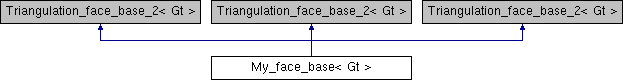
\includegraphics[height=1.786284cm]{classMy__face__base}
\end{center}
\end{figure}
\subsubsection*{Public Member Functions}
\begin{DoxyCompactItemize}
\item 
{\bfseries My\+\_\+face\+\_\+base} (void $\ast$v0, void $\ast$v1, void $\ast$v2)\hypertarget{classMy__face__base_a0af70fd60f0aed9b024b89ea6a81d301}{}\label{classMy__face__base_a0af70fd60f0aed9b024b89ea6a81d301}

\item 
{\bfseries My\+\_\+face\+\_\+base} (void $\ast$v0, void $\ast$v1, void $\ast$v2, void $\ast$n0, void $\ast$n1, void $\ast$n2)\hypertarget{classMy__face__base_aec3abe8ca3bec335a5d865fa8c7fe8f3}{}\label{classMy__face__base_aec3abe8ca3bec335a5d865fa8c7fe8f3}

\item 
{\bfseries My\+\_\+face\+\_\+base} (void $\ast$v0, void $\ast$v1, void $\ast$v2)\hypertarget{classMy__face__base_a0af70fd60f0aed9b024b89ea6a81d301}{}\label{classMy__face__base_a0af70fd60f0aed9b024b89ea6a81d301}

\item 
{\bfseries My\+\_\+face\+\_\+base} (void $\ast$v0, void $\ast$v1, void $\ast$v2, void $\ast$n0, void $\ast$n1, void $\ast$n2)\hypertarget{classMy__face__base_aec3abe8ca3bec335a5d865fa8c7fe8f3}{}\label{classMy__face__base_aec3abe8ca3bec335a5d865fa8c7fe8f3}

\item 
{\bfseries My\+\_\+face\+\_\+base} (void $\ast$v0, void $\ast$v1, void $\ast$v2)\hypertarget{classMy__face__base_a0af70fd60f0aed9b024b89ea6a81d301}{}\label{classMy__face__base_a0af70fd60f0aed9b024b89ea6a81d301}

\item 
{\bfseries My\+\_\+face\+\_\+base} (void $\ast$v0, void $\ast$v1, void $\ast$v2, void $\ast$n0, void $\ast$n1, void $\ast$n2)\hypertarget{classMy__face__base_aec3abe8ca3bec335a5d865fa8c7fe8f3}{}\label{classMy__face__base_aec3abe8ca3bec335a5d865fa8c7fe8f3}

\end{DoxyCompactItemize}
\subsubsection*{Public Attributes}
\begin{DoxyCompactItemize}
\item 
Color {\bfseries color}\hypertarget{classMy__face__base_aefc38372916d172f9b1ef5bd996a1718}{}\label{classMy__face__base_aefc38372916d172f9b1ef5bd996a1718}

\item 
C\+G\+A\+L\+::\+Color {\bfseries color}\hypertarget{classMy__face__base_aefc38372916d172f9b1ef5bd996a1718}{}\label{classMy__face__base_aefc38372916d172f9b1ef5bd996a1718}

\end{DoxyCompactItemize}


\subsubsection{Detailed Description}
\subsubsection*{template$<$class Gt$>$\\*
class My\+\_\+face\+\_\+base$<$ Gt $>$}



Definition at line 26 of file Var\+Data\+C\+G\+A\+L.\+cpp.



The documentation for this class was generated from the following files\+:\begin{DoxyCompactItemize}
\item 
src/\+Var\+Data/Var\+Data\+C\+G\+A\+L.\+cpp\item 
src/\+El\+Poly/El\+Poly\+Draw\+C\+G\+A\+L.\+cpp\item 
src/\+El\+Poly/El\+Poly\+Draw\+Triang\+C\+G\+A\+L.\+cpp\end{DoxyCompactItemize}

\hypertarget{structNANO}{\subsection{\-N\-A\-N\-O \-Struct \-Reference}
\label{structNANO}\index{\-N\-A\-N\-O@{\-N\-A\-N\-O}}
}


\-Information about the nanoparticle.  




{\ttfamily \#include $<$\-Var\-Data.\-h$>$}

\subsubsection*{\-Public \-Attributes}
\begin{DoxyCompactItemize}
\item 
\hypertarget{structNANO_a750f14eafb9dc7737d8524501eeef457}{char \hyperlink{structNANO_a750f14eafb9dc7737d8524501eeef457}{\-Arch\-File} \mbox{[}60\mbox{]}}\label{structNANO_a750f14eafb9dc7737d8524501eeef457}

\begin{DoxyCompactList}\small\item\em \-Architecture file. \end{DoxyCompactList}\item 
\hypertarget{structNANO_a863738e46f14b3bfc674ad87d35f143d}{double \hyperlink{structNANO_a863738e46f14b3bfc674ad87d35f143d}{\-Pos} \mbox{[}3\mbox{]}}\label{structNANO_a863738e46f14b3bfc674ad87d35f143d}

\begin{DoxyCompactList}\small\item\em \-Position. \end{DoxyCompactList}\item 
\hypertarget{structNANO_a77abbc20fd99f1fb464e7a922e543e19}{double \hyperlink{structNANO_a77abbc20fd99f1fb464e7a922e543e19}{\-Bkf} \mbox{[}3\mbox{]}}\label{structNANO_a77abbc20fd99f1fb464e7a922e543e19}

\begin{DoxyCompactList}\small\item\em \-Backfolded position. \end{DoxyCompactList}\item 
\hypertarget{structNANO_ae3fae9edc78d8cadc33c5a52bebdb46c}{double \hyperlink{structNANO_ae3fae9edc78d8cadc33c5a52bebdb46c}{\-Vel} \mbox{[}3\mbox{]}}\label{structNANO_ae3fae9edc78d8cadc33c5a52bebdb46c}

\begin{DoxyCompactList}\small\item\em \-Velocity. \end{DoxyCompactList}\item 
\hypertarget{structNANO_ad597aadcc443ffa959ac837ba5382bff}{double \hyperlink{structNANO_ad597aadcc443ffa959ac837ba5382bff}{\-Force} \mbox{[}3\mbox{]}}\label{structNANO_ad597aadcc443ffa959ac837ba5382bff}

\begin{DoxyCompactList}\small\item\em \hyperlink{classForces}{\-Forces}. \end{DoxyCompactList}\item 
\hypertarget{structNANO_a953bf4fe7bc5cd9cffa0f049f7fb0325}{double \hyperlink{structNANO_a953bf4fe7bc5cd9cffa0f049f7fb0325}{\-Axis} \mbox{[}3\mbox{]}}\label{structNANO_a953bf4fe7bc5cd9cffa0f049f7fb0325}

\begin{DoxyCompactList}\small\item\em \-Rotation axis. \end{DoxyCompactList}\item 
\hypertarget{structNANO_ad1bdf13b47e2dca8f97d3807e3adf840}{double \hyperlink{structNANO_ad1bdf13b47e2dca8f97d3807e3adf840}{\-A\-Mom} \mbox{[}3\mbox{]}}\label{structNANO_ad1bdf13b47e2dca8f97d3807e3adf840}

\begin{DoxyCompactList}\small\item\em \-Angular momentum. \end{DoxyCompactList}\item 
\hypertarget{structNANO_a062cb4da9ccaf4fe931d0262f827c8c3}{double \hyperlink{structNANO_a062cb4da9ccaf4fe931d0262f827c8c3}{\-A\-Mom\-Temp} \mbox{[}3\mbox{]}}\label{structNANO_a062cb4da9ccaf4fe931d0262f827c8c3}

\begin{DoxyCompactList}\small\item\em \-Temporal angular momentum. \end{DoxyCompactList}\item 
\hypertarget{structNANO_a27de9c01526ba1025ed85f899b3fbc74}{double \hyperlink{structNANO_a27de9c01526ba1025ed85f899b3fbc74}{\-A\-Vel} \mbox{[}3\mbox{]}}\label{structNANO_a27de9c01526ba1025ed85f899b3fbc74}

\begin{DoxyCompactList}\small\item\em \-Angular velocity. \end{DoxyCompactList}\item 
\hypertarget{structNANO_ac33418187547ea28dda7063924f34df6}{double \hyperlink{structNANO_ac33418187547ea28dda7063924f34df6}{\-Mass}}\label{structNANO_ac33418187547ea28dda7063924f34df6}

\begin{DoxyCompactList}\small\item\em \-Mass. \end{DoxyCompactList}\item 
\hypertarget{structNANO_a860bef50013f57ab1a6437b7986a9487}{double \hyperlink{structNANO_a860bef50013f57ab1a6437b7986a9487}{\-Rad}}\label{structNANO_a860bef50013f57ab1a6437b7986a9487}

\begin{DoxyCompactList}\small\item\em \-Size. \end{DoxyCompactList}\item 
\hypertarget{structNANO_a2c39c1efe4f21bf1103d46b0a4e8f5a9}{double \hyperlink{structNANO_a2c39c1efe4f21bf1103d46b0a4e8f5a9}{\-Hamaker}}\label{structNANO_a2c39c1efe4f21bf1103d46b0a4e8f5a9}

\begin{DoxyCompactList}\small\item\em \-Strength of the interaction. \end{DoxyCompactList}\item 
\hypertarget{structNANO_a18ece2127f70c26ead73bc24856a5c57}{double \hyperlink{structNANO_a18ece2127f70c26ead73bc24856a5c57}{\-Height}}\label{structNANO_a18ece2127f70c26ead73bc24856a5c57}

\begin{DoxyCompactList}\small\item\em \-Height of the cylinder. \end{DoxyCompactList}\item 
\hypertarget{structNANO_a1a0cbbb118b67bb2a3f1f682c0dad85b}{double \hyperlink{structNANO_a1a0cbbb118b67bb2a3f1f682c0dad85b}{\-Gamma}}\label{structNANO_a1a0cbbb118b67bb2a3f1f682c0dad85b}

\begin{DoxyCompactList}\small\item\em \-Friction term. \end{DoxyCompactList}\item 
\hypertarget{structNANO_a7e97ac28698cae83ebf4b304dbbae40a}{double \hyperlink{structNANO_a7e97ac28698cae83ebf4b304dbbae40a}{\-Zeta}}\label{structNANO_a7e97ac28698cae83ebf4b304dbbae40a}

\begin{DoxyCompactList}\small\item\em \-Stochastic term. \end{DoxyCompactList}\item 
\hypertarget{structNANO_a0846f0b0f68bb4cbe7b44d53f6200139}{double \hyperlink{structNANO_a0846f0b0f68bb4cbe7b44d53f6200139}{\-Viscosity}}\label{structNANO_a0846f0b0f68bb4cbe7b44d53f6200139}

\begin{DoxyCompactList}\small\item\em \-Viscosity. \end{DoxyCompactList}\item 
\hypertarget{structNANO_a78d4e3879bef31479e4cbfe231746de0}{double \hyperlink{structNANO_a78d4e3879bef31479e4cbfe231746de0}{\-Off\-Set}}\label{structNANO_a78d4e3879bef31479e4cbfe231746de0}

\begin{DoxyCompactList}\small\item\em \-Reference potential. \end{DoxyCompactList}\item 
\hypertarget{structNANO_af2411aba2dd63fa22b1bc279653ff7a0}{double \hyperlink{structNANO_af2411aba2dd63fa22b1bc279653ff7a0}{\-Cut\-Off}}\label{structNANO_af2411aba2dd63fa22b1bc279653ff7a0}

\begin{DoxyCompactList}\small\item\em \-Cut off of the potential. \end{DoxyCompactList}\item 
\hypertarget{structNANO_a33ea180d74655fd48d17ae1b6ff1236d}{double \hyperlink{structNANO_a33ea180d74655fd48d17ae1b6ff1236d}{\-Coating}}\label{structNANO_a33ea180d74655fd48d17ae1b6ff1236d}

\begin{DoxyCompactList}\small\item\em \-Thickness of the \-L\-J well. \end{DoxyCompactList}\item 
\hypertarget{structNANO_a12346a80b6dd9472f0a10aab633f2f4f}{double \hyperlink{structNANO_a12346a80b6dd9472f0a10aab633f2f4f}{\-Base\-Line}}\label{structNANO_a12346a80b6dd9472f0a10aab633f2f4f}

\begin{DoxyCompactList}\small\item\em \-Baseline of the potential. \end{DoxyCompactList}\item 
\hypertarget{structNANO_a7be87fae5fde1648d34b194775515d08}{double \hyperlink{structNANO_a7be87fae5fde1648d34b194775515d08}{\-Dist\-Thr}}\label{structNANO_a7be87fae5fde1648d34b194775515d08}

\begin{DoxyCompactList}\small\item\em \-Minimum distance threshold. \end{DoxyCompactList}\item 
\hypertarget{structNANO_ad631a0b43047f95f5bb991f5407b813e}{double \hyperlink{structNANO_ad631a0b43047f95f5bb991f5407b813e}{\-For\-Thr}}\label{structNANO_ad631a0b43047f95f5bb991f5407b813e}

\begin{DoxyCompactList}\small\item\em \-Maximum value of the force. \end{DoxyCompactList}\item 
\hypertarget{structNANO_adf3d7e8b11ee1fa9f6b7b58141ab5112}{double \hyperlink{structNANO_adf3d7e8b11ee1fa9f6b7b58141ab5112}{\-Pot\-Thr}}\label{structNANO_adf3d7e8b11ee1fa9f6b7b58141ab5112}

\begin{DoxyCompactList}\small\item\em \-Maximum value of the potential. \end{DoxyCompactList}\item 
\hypertarget{structNANO_acedb30173c5224396eb7a95709f5c619}{double \hyperlink{structNANO_acedb30173c5224396eb7a95709f5c619}{\-Area}}\label{structNANO_acedb30173c5224396eb7a95709f5c619}

\begin{DoxyCompactList}\small\item\em \-Area of a pore or a stalk. \end{DoxyCompactList}\item 
\hypertarget{structNANO_ae10d368b167a39a5905e047ba7083b2a}{int \hyperlink{structNANO_ae10d368b167a39a5905e047ba7083b2a}{\-Shape}}\label{structNANO_ae10d368b167a39a5905e047ba7083b2a}

\begin{DoxyCompactList}\small\item\em 0 none, 1 spherical, 2 cylindrical 3 wall \end{DoxyCompactList}\item 
\hypertarget{structNANO_a73918a2decc99bcf2317d2855dada6c8}{int \hyperlink{structNANO_a73918a2decc99bcf2317d2855dada6c8}{\-N\-Link}}\label{structNANO_a73918a2decc99bcf2317d2855dada6c8}

\begin{DoxyCompactList}\small\item\em \-Number of links connecting the constituent monomers. \end{DoxyCompactList}\item 
\hypertarget{structNANO_a03b74f589ea1f823e1a80cf00b6dde33}{int \hyperlink{structNANO_a03b74f589ea1f823e1a80cf00b6dde33}{\-N\-Height}}\label{structNANO_a03b74f589ea1f823e1a80cf00b6dde33}

\begin{DoxyCompactList}\small\item\em \-Number of monomers per side. \end{DoxyCompactList}\item 
\hypertarget{structNANO_a74ded76c210b56e54322eeeb9be4dc6e}{int \hyperlink{structNANO_a74ded76c210b56e54322eeeb9be4dc6e}{\-N\-Circle}}\label{structNANO_a74ded76c210b56e54322eeeb9be4dc6e}

\begin{DoxyCompactList}\small\item\em \-Number of monomers per circle. \end{DoxyCompactList}\item 
\hypertarget{structNANO_a41bd38e6447756bd59b0f61559fa57ce}{int \hyperlink{structNANO_a41bd38e6447756bd59b0f61559fa57ce}{n\-Block}}\label{structNANO_a41bd38e6447756bd59b0f61559fa57ce}

\begin{DoxyCompactList}\small\item\em \-In which block is the peptide written. \end{DoxyCompactList}\end{DoxyCompactItemize}


\subsubsection{\-Detailed \-Description}
\-Information about the nanoparticle. 

\-Definition at line 423 of file \-Var\-Data.\-h.



\-The documentation for this struct was generated from the following file\-:\begin{DoxyCompactItemize}
\item 
include/\-Var\-Data.\-h\end{DoxyCompactItemize}

\hypertarget{classNeiVertex}{\subsection{\-Nei\-Vertex \-Class \-Reference}
\label{classNeiVertex}\index{\-Nei\-Vertex@{\-Nei\-Vertex}}
}


\-Connects the triangles by vertices.  




{\ttfamily \#include $<$\-Cubo.\-h$>$}

\subsubsection*{\-Public \-Member \-Functions}
\begin{DoxyCompactItemize}
\item 
\hypertarget{classNeiVertex_acd292e575bf4ade488a69f62b2d454ad}{\hyperlink{classNeiVertex_acd292e575bf4ade488a69f62b2d454ad}{\-Nei\-Vertex} (int \-N\-Tria\-Ext, int \-Nv\-Pt\-Ext, int \-N\-Grid\-Ext, double $\ast$\-Edge\-Ext)}\label{classNeiVertex_acd292e575bf4ade488a69f62b2d454ad}

\begin{DoxyCompactList}\small\item\em \-Alloc \-N\-Vertices. \end{DoxyCompactList}\item 
\hypertarget{classNeiVertex_ab53f242febf6312ccd82ee9c28c2b633}{\hyperlink{classNeiVertex_ab53f242febf6312ccd82ee9c28c2b633}{$\sim$\-Nei\-Vertex} ()}\label{classNeiVertex_ab53f242febf6312ccd82ee9c28c2b633}

\begin{DoxyCompactList}\small\item\em \-Delete the class. \end{DoxyCompactList}\item 
\hypertarget{classNeiVertex_ab46ead706c925650dc870081c73da25f}{void \hyperlink{classNeiVertex_ab46ead706c925650dc870081c73da25f}{\-Add} (int v, int t, double $\ast$\-Pos)}\label{classNeiVertex_ab46ead706c925650dc870081c73da25f}

\begin{DoxyCompactList}\small\item\em \-Add the triangle t at the vertex v. \end{DoxyCompactList}\item 
\hypertarget{classNeiVertex_a23175dfa70c692054cf173193a6d4d6e}{void \hyperlink{classNeiVertex_a23175dfa70c692054cf173193a6d4d6e}{\-Add} (double $\ast$\-Pos, int t)}\label{classNeiVertex_a23175dfa70c692054cf173193a6d4d6e}

\begin{DoxyCompactList}\small\item\em \-Add the triangle t in the \-Pos. \end{DoxyCompactList}\item 
\hypertarget{classNeiVertex_a8c5cc8bfb6783d235a0b273821f5e475}{void \hyperlink{classNeiVertex_a8c5cc8bfb6783d235a0b273821f5e475}{\-Rem} (int v, int t)}\label{classNeiVertex_a8c5cc8bfb6783d235a0b273821f5e475}

\begin{DoxyCompactList}\small\item\em \-Remove the triangle t from the vertex v. \end{DoxyCompactList}\item 
\hypertarget{classNeiVertex_a2be4fa5175ea113c1762d2a4cbc21091}{void \hyperlink{classNeiVertex_a2be4fa5175ea113c1762d2a4cbc21091}{\-Copy\-Vert2\-To1} (\hyperlink{structVERTEX}{\-V\-E\-R\-T\-E\-X} \-Vert1, \hyperlink{structVERTEX}{\-V\-E\-R\-T\-E\-X} \-Vert2)}\label{classNeiVertex_a2be4fa5175ea113c1762d2a4cbc21091}

\begin{DoxyCompactList}\small\item\em \-Copy two vertices. \end{DoxyCompactList}\item 
\hypertarget{classNeiVertex_aa22b5926829059f1b8f5ee084497f2ab}{void \hyperlink{classNeiVertex_aa22b5926829059f1b8f5ee084497f2ab}{\-Swap} (int v1, int v2)}\label{classNeiVertex_aa22b5926829059f1b8f5ee084497f2ab}

\begin{DoxyCompactList}\small\item\em \-Swap to vertices. \end{DoxyCompactList}\item 
\hypertarget{classNeiVertex_aeeb3068ff4b57530bda6a4f1180fe383}{void \hyperlink{classNeiVertex_aeeb3068ff4b57530bda6a4f1180fe383}{\-Reorder} ()}\label{classNeiVertex_aeeb3068ff4b57530bda6a4f1180fe383}

\begin{DoxyCompactList}\small\item\em \-Reorder and fill the vertices. \end{DoxyCompactList}\item 
void \hyperlink{classNeiVertex_a86a3208513ff31c3391998f4900f52b5}{\-Set\-Counters} (int v)
\begin{DoxyCompactList}\small\item\em \-Set counters to zero for the point v. \end{DoxyCompactList}\item 
\hypertarget{classNeiVertex_a7c3a47a119b3c06d24a0c8a370fef66c}{void \hyperlink{classNeiVertex_a7c3a47a119b3c06d24a0c8a370fef66c}{\-Set\-Counters} ()}\label{classNeiVertex_a7c3a47a119b3c06d24a0c8a370fef66c}

\begin{DoxyCompactList}\small\item\em \-Set all the counters to zero. \end{DoxyCompactList}\item 
\hypertarget{classNeiVertex_a330eb7ef3b6ff289f9428fd4994209af}{int \hyperlink{classNeiVertex_a330eb7ef3b6ff289f9428fd4994209af}{\-Get\-Vertex} (double $\ast$\-Pos)}\label{classNeiVertex_a330eb7ef3b6ff289f9428fd4994209af}

\begin{DoxyCompactList}\small\item\em \-Correspondent vertes for \-Pos. \end{DoxyCompactList}\item 
\hypertarget{classNeiVertex_adb170c151213885180aba70f23ac7452}{int \hyperlink{classNeiVertex_adb170c151213885180aba70f23ac7452}{\-If\-It\-Cell} (int v)}\label{classNeiVertex_adb170c151213885180aba70f23ac7452}

\begin{DoxyCompactList}\small\item\em \-End of the counters. \end{DoxyCompactList}\item 
\hypertarget{classNeiVertex_afefd8d5278268d8224caba5312860e5d}{void \hyperlink{classNeiVertex_afefd8d5278268d8224caba5312860e5d}{\-Incr\-Curr} (int v)}\label{classNeiVertex_afefd8d5278268d8224caba5312860e5d}

\begin{DoxyCompactList}\small\item\em \-Increment the counter. \end{DoxyCompactList}\item 
\hypertarget{classNeiVertex_a072488de60aa6fce524b79855cb53ec5}{int \hyperlink{classNeiVertex_a072488de60aa6fce524b79855cb53ec5}{\-Vert\-Curr} (int v)}\label{classNeiVertex_a072488de60aa6fce524b79855cb53ec5}

\begin{DoxyCompactList}\small\item\em \-Current vertex iterator for the vertex v. \end{DoxyCompactList}\item 
\hypertarget{classNeiVertex_aebbce34f5213484c16fe08591fe0f8d7}{int \hyperlink{classNeiVertex_aebbce34f5213484c16fe08591fe0f8d7}{\-Tria\-Curr} (int v)}\label{classNeiVertex_aebbce34f5213484c16fe08591fe0f8d7}

\begin{DoxyCompactList}\small\item\em \-Current triangle for the vertex v. \end{DoxyCompactList}\item 
\hypertarget{classNeiVertex_a81093b4cb48a3e1598c724287c410a9d}{void \hyperlink{classNeiVertex_a81093b4cb48a3e1598c724287c410a9d}{\-Pos\-Vertex} (int v, double $\ast$\-Pos)}\label{classNeiVertex_a81093b4cb48a3e1598c724287c410a9d}

\begin{DoxyCompactList}\small\item\em \-Position of the vertex v. \end{DoxyCompactList}\item 
\hypertarget{classNeiVertex_a9dcac18006ce057b8d78c847174c1362}{void \hyperlink{classNeiVertex_a9dcac18006ce057b8d78c847174c1362}{\-Print} ()}\label{classNeiVertex_a9dcac18006ce057b8d78c847174c1362}

\begin{DoxyCompactList}\small\item\em \-Print the entire structure. \end{DoxyCompactList}\end{DoxyCompactItemize}


\subsubsection{\-Detailed \-Description}
\-Connects the triangles by vertices. 

\-Definition at line 480 of file \-Cubo.\-h.



\subsubsection{\-Member \-Function \-Documentation}
\hypertarget{classNeiVertex_a86a3208513ff31c3391998f4900f52b5}{\index{\-Nei\-Vertex@{\-Nei\-Vertex}!\-Set\-Counters@{\-Set\-Counters}}
\index{\-Set\-Counters@{\-Set\-Counters}!NeiVertex@{\-Nei\-Vertex}}
\paragraph[{\-Set\-Counters}]{\setlength{\rightskip}{0pt plus 5cm}void {\bf \-Set\-Counters} (
\begin{DoxyParamCaption}
\item[{int}]{v}
\end{DoxyParamCaption}
)}}\label{classNeiVertex_a86a3208513ff31c3391998f4900f52b5}


\-Set counters to zero for the point v. 

\-Initialize the. 

\-Definition at line 1093 of file \-Cubo.\-cpp.



\-Referenced by \-Var\-Data\-::\-Connect\-Line\-Chain2(), and \-Var\-Data\-::\-Normal\-Weight().



\-The documentation for this class was generated from the following files\-:\begin{DoxyCompactItemize}
\item 
include/\-Cubo.\-h\item 
src/\-Var\-Data/\-Cubo.\-cpp\item 
src/\-Var\-Data/\-Cubo.\-mirror.\-cpp\end{DoxyCompactItemize}

\hypertarget{structPARABOLA}{\subsection{\-P\-A\-R\-A\-B\-O\-L\-A \-Struct \-Reference}
\label{structPARABOLA}\index{\-P\-A\-R\-A\-B\-O\-L\-A@{\-P\-A\-R\-A\-B\-O\-L\-A}}
}


\-Parabolas coefficients.  




{\ttfamily \#include $<$\-Matematica\-Struct.\-h$>$}

\subsubsection*{\-Public \-Attributes}
\begin{DoxyCompactItemize}
\item 
\hypertarget{structPARABOLA_ad95dcba445836b4ba94129111a4b888c}{double \hyperlink{structPARABOLA_ad95dcba445836b4ba94129111a4b888c}{a0}}\label{structPARABOLA_ad95dcba445836b4ba94129111a4b888c}

\begin{DoxyCompactList}\small\item\em a0 + a1 x + a2 x$^\wedge$2 \end{DoxyCompactList}\item 
\hypertarget{structPARABOLA_adc871ead9d8fc23f2009f42306b04a5e}{double \hyperlink{structPARABOLA_adc871ead9d8fc23f2009f42306b04a5e}{\-Erra0}}\label{structPARABOLA_adc871ead9d8fc23f2009f42306b04a5e}

\begin{DoxyCompactList}\small\item\em \-Error on the first coefficient. \end{DoxyCompactList}\item 
\hypertarget{structPARABOLA_a5d015a3751aec61f2442b957cb6f517a}{double \hyperlink{structPARABOLA_a5d015a3751aec61f2442b957cb6f517a}{a1}}\label{structPARABOLA_a5d015a3751aec61f2442b957cb6f517a}

\begin{DoxyCompactList}\small\item\em a0 + a1 x + a2 x$^\wedge$2 \end{DoxyCompactList}\item 
\hypertarget{structPARABOLA_a9097314f53ed21d9ca0286f35e86d82d}{double \hyperlink{structPARABOLA_a9097314f53ed21d9ca0286f35e86d82d}{\-Erra1}}\label{structPARABOLA_a9097314f53ed21d9ca0286f35e86d82d}

\begin{DoxyCompactList}\small\item\em \-Error on the second coefficient. \end{DoxyCompactList}\item 
\hypertarget{structPARABOLA_ac55c2d269ed76bd9bdb7fb25f3533a4e}{double \hyperlink{structPARABOLA_ac55c2d269ed76bd9bdb7fb25f3533a4e}{a2}}\label{structPARABOLA_ac55c2d269ed76bd9bdb7fb25f3533a4e}

\begin{DoxyCompactList}\small\item\em a0 + a1 x + a2 x$^\wedge$2 \end{DoxyCompactList}\item 
\hypertarget{structPARABOLA_a18371909b4059cce673620670d516e01}{double \hyperlink{structPARABOLA_a18371909b4059cce673620670d516e01}{\-Erra2}}\label{structPARABOLA_a18371909b4059cce673620670d516e01}

\begin{DoxyCompactList}\small\item\em \-Error on the third coefficient. \end{DoxyCompactList}\item 
\hypertarget{structPARABOLA_a09d69325016439f54c434a28a71bf666}{double \hyperlink{structPARABOLA_a09d69325016439f54c434a28a71bf666}{\-Minimo}}\label{structPARABOLA_a09d69325016439f54c434a28a71bf666}

\begin{DoxyCompactList}\small\item\em \-Minimum of the parabola. \end{DoxyCompactList}\item 
\hypertarget{structPARABOLA_abbfab7a69ef1371aef5bf3cefa0abaa9}{double \hyperlink{structPARABOLA_abbfab7a69ef1371aef5bf3cefa0abaa9}{\-Minimo\-Y}}\label{structPARABOLA_abbfab7a69ef1371aef5bf3cefa0abaa9}

\begin{DoxyCompactList}\small\item\em \-Minimum of the parabola. \end{DoxyCompactList}\end{DoxyCompactItemize}


\subsubsection{\-Detailed \-Description}
\-Parabolas coefficients. 

\-Definition at line 7 of file \-Matematica\-Struct.\-h.



\-The documentation for this struct was generated from the following file\-:\begin{DoxyCompactItemize}
\item 
include/\-Matematica\-Struct.\-h\end{DoxyCompactItemize}

\hypertarget{structPART}{\subsection{\-P\-A\-R\-T \-Struct \-Reference}
\label{structPART}\index{\-P\-A\-R\-T@{\-P\-A\-R\-T}}
}


\-Information of every particle.  




{\ttfamily \#include $<$\-Var\-Data.\-h$>$}

\subsubsection*{\-Public \-Attributes}
\begin{DoxyCompactItemize}
\item 
\hypertarget{structPART_a863738e46f14b3bfc674ad87d35f143d}{double \hyperlink{structPART_a863738e46f14b3bfc674ad87d35f143d}{\-Pos} \mbox{[}3\mbox{]}}\label{structPART_a863738e46f14b3bfc674ad87d35f143d}

\begin{DoxyCompactList}\small\item\em xyz \-Position of the particle \end{DoxyCompactList}\item 
\hypertarget{structPART_a77abbc20fd99f1fb464e7a922e543e19}{double \hyperlink{structPART_a77abbc20fd99f1fb464e7a922e543e19}{\-Bkf} \mbox{[}3\mbox{]}}\label{structPART_a77abbc20fd99f1fb464e7a922e543e19}

\begin{DoxyCompactList}\small\item\em xyz \-Backfold distance \end{DoxyCompactList}\item 
\hypertarget{structPART_afd1b3747170c238c06ba3420cbc5c2a2}{double \hyperlink{structPART_afd1b3747170c238c06ba3420cbc5c2a2}{\-Vel} \mbox{[}4\mbox{]}}\label{structPART_afd1b3747170c238c06ba3420cbc5c2a2}

\begin{DoxyCompactList}\small\item\em xyzr \-Velocity of the particle \end{DoxyCompactList}\item 
\hypertarget{structPART_a26c51826a2d187b6baa0f5f249436abe}{int \hyperlink{structPART_a26c51826a2d187b6baa0f5f249436abe}{\-Idx}}\label{structPART_a26c51826a2d187b6baa0f5f249436abe}

\begin{DoxyCompactList}\small\item\em \-Particle identifier. \end{DoxyCompactList}\item 
\hypertarget{structPART_ae9c6df97c72d6a4af74acf24adbe81bf}{int \hyperlink{structPART_ae9c6df97c72d6a4af74acf24adbe81bf}{\-C\-Id}}\label{structPART_ae9c6df97c72d6a4af74acf24adbe81bf}

\begin{DoxyCompactList}\small\item\em \-Chain \-Identifier. \end{DoxyCompactList}\item 
\hypertarget{structPART_a6365019ac3c6ee60c2db6a3674f35614}{int \hyperlink{structPART_a6365019ac3c6ee60c2db6a3674f35614}{\-Typ}}\label{structPART_a6365019ac3c6ee60c2db6a3674f35614}

\begin{DoxyCompactList}\small\item\em \-Type. \end{DoxyCompactList}\end{DoxyCompactItemize}


\subsubsection{\-Detailed \-Description}
\-Information of every particle. 

\-Definition at line 214 of file \-Var\-Data.\-h.



\-The documentation for this struct was generated from the following file\-:\begin{DoxyCompactItemize}
\item 
include/\-Var\-Data.\-h\end{DoxyCompactItemize}

\hypertarget{structPERMUTE}{\subsection{\-P\-E\-R\-M\-U\-T\-E \-Struct \-Reference}
\label{structPERMUTE}\index{\-P\-E\-R\-M\-U\-T\-E@{\-P\-E\-R\-M\-U\-T\-E}}
}


\-Indices for the permutation.  




{\ttfamily \#include $<$\-Matematica\-Struct.\-h$>$}

\subsubsection*{\-Public \-Attributes}
\begin{DoxyCompactItemize}
\item 
\hypertarget{structPERMUTE_a76f11d9a0a47b94f72c2d0e77fb32240}{int \hyperlink{structPERMUTE_a76f11d9a0a47b94f72c2d0e77fb32240}{n}}\label{structPERMUTE_a76f11d9a0a47b94f72c2d0e77fb32240}

\begin{DoxyCompactList}\small\item\em \-First number of the couple. \end{DoxyCompactList}\item 
\hypertarget{structPERMUTE_a742204794ea328ba293fe59cec79b990}{int \hyperlink{structPERMUTE_a742204794ea328ba293fe59cec79b990}{m}}\label{structPERMUTE_a742204794ea328ba293fe59cec79b990}

\begin{DoxyCompactList}\small\item\em \-Second number of the couple. \end{DoxyCompactList}\end{DoxyCompactItemize}


\subsubsection{\-Detailed \-Description}
\-Indices for the permutation. 

\-Definition at line 97 of file \-Matematica\-Struct.\-h.



\-The documentation for this struct was generated from the following file\-:\begin{DoxyCompactItemize}
\item 
include/\-Matematica\-Struct.\-h\end{DoxyCompactItemize}

\hypertarget{classPiano}{\subsection{\-Piano \-Class \-Reference}
\label{classPiano}\index{\-Piano@{\-Piano}}
}


\-Define a plane.  




{\ttfamily \#include $<$\-Matematica\-Plane.\-h$>$}

\subsubsection*{\-Public \-Member \-Functions}
\begin{DoxyCompactItemize}
\item 
\hypertarget{classPiano_a3e0f72f2e5410fb6ac0994b962e3b0f4}{\hyperlink{classPiano_a3e0f72f2e5410fb6ac0994b962e3b0f4}{\-Piano} (\hyperlink{classVettore}{\-Vettore} $\ast$\hyperlink{classPiano_aca046e5963a53f1b4a12c2ad4617149b}{\-P1}, \hyperlink{classVettore}{\-Vettore} $\ast$\-P2, \hyperlink{classVettore}{\-Vettore} $\ast$\-P3)}\label{classPiano_a3e0f72f2e5410fb6ac0994b962e3b0f4}

\begin{DoxyCompactList}\small\item\em \-Allocates. \end{DoxyCompactList}\item 
\hypertarget{classPiano_ae2f8ebc5dd8ecab651c1e8a0551ec11d}{\hyperlink{classPiano_ae2f8ebc5dd8ecab651c1e8a0551ec11d}{$\sim$\-Piano} ()}\label{classPiano_ae2f8ebc5dd8ecab651c1e8a0551ec11d}

\begin{DoxyCompactList}\small\item\em \-Frees. \end{DoxyCompactList}\item 
\hypertarget{classPiano_a8ec22e845b3d00f3a815a132132fc9a1}{double \hyperlink{classPiano_a8ec22e845b3d00f3a815a132132fc9a1}{\-Distance} (\hyperlink{classVettore}{\-Vettore} $\ast$\-P)}\label{classPiano_a8ec22e845b3d00f3a815a132132fc9a1}

\begin{DoxyCompactList}\small\item\em \-Distance. \end{DoxyCompactList}\item 
\hypertarget{classPiano_a119e25248ace7e082367a7b64e3bcbc1}{int \hyperlink{classPiano_a119e25248ace7e082367a7b64e3bcbc1}{\-Impact} (\hyperlink{classVettore}{\-Vettore} $\ast$\-P, \hyperlink{classVettore}{\-Vettore} $\ast$\-V)}\label{classPiano_a119e25248ace7e082367a7b64e3bcbc1}

\begin{DoxyCompactList}\small\item\em \-Reflect velocity. \end{DoxyCompactList}\item 
\hypertarget{classPiano_a1c0e56e45b12255147f5cbbc5a8e0b1f}{\hyperlink{classVettore}{\-Vettore} \hyperlink{classPiano_a1c0e56e45b12255147f5cbbc5a8e0b1f}{\-Get\-Vertex} (int i)}\label{classPiano_a1c0e56e45b12255147f5cbbc5a8e0b1f}

\begin{DoxyCompactList}\small\item\em \-Get vertex. \end{DoxyCompactList}\item 
\hypertarget{classPiano_a4aedb9029e37fb894e1e3a4514e4707d}{\hyperlink{classVettore}{\-Vettore} \hyperlink{classPiano_a4aedb9029e37fb894e1e3a4514e4707d}{\-Proj\-On\-Surf} (\hyperlink{classVettore}{\-Vettore} $\ast$\-Pos)}\label{classPiano_a4aedb9029e37fb894e1e3a4514e4707d}

\begin{DoxyCompactList}\small\item\em \-Project on surface (point) \end{DoxyCompactList}\item 
\hypertarget{classPiano_af86bbe20f8d523af9e2553f0039c088b}{\hyperlink{classVettore}{\-Vettore} \hyperlink{classPiano_af86bbe20f8d523af9e2553f0039c088b}{\-Proj\-On\-Norm} (\hyperlink{classVettore}{\-Vettore} $\ast$v)}\label{classPiano_af86bbe20f8d523af9e2553f0039c088b}

\begin{DoxyCompactList}\small\item\em \-Project on normal (vector) \end{DoxyCompactList}\item 
\hypertarget{classPiano_a07236f42214a9066ed4c12a8b62ada12}{int \hyperlink{classPiano_a07236f42214a9066ed4c12a8b62ada12}{\-Same\-Side} (\hyperlink{classVettore}{\-Vettore} $\ast$\-P, \hyperlink{classVettore}{\-Vettore} $\ast$\-A, \hyperlink{classVettore}{\-Vettore} $\ast$\-B, \hyperlink{classVettore}{\-Vettore} $\ast$\-C)}\label{classPiano_a07236f42214a9066ed4c12a8b62ada12}

\begin{DoxyCompactList}\small\item\em \-Is the orientation of the difference vectors on the same side? \end{DoxyCompactList}\item 
\hypertarget{classPiano_a9341053ea31914d454cab1a86e2f8dd9}{double \hyperlink{classPiano_a9341053ea31914d454cab1a86e2f8dd9}{\-Inv} (double x)}\label{classPiano_a9341053ea31914d454cab1a86e2f8dd9}

\begin{DoxyCompactList}\small\item\em \-Calculate the inverse. \end{DoxyCompactList}\item 
\hypertarget{classPiano_ad605fc62ded454a95190f42608532c64}{int \hyperlink{classPiano_ad605fc62ded454a95190f42608532c64}{\-Is\-On\-Surf} (\hyperlink{classVettore}{\-Vettore} $\ast$\-P)}\label{classPiano_ad605fc62ded454a95190f42608532c64}

\begin{DoxyCompactList}\small\item\em \-If the point is inside the triangle. \end{DoxyCompactList}\item 
\hypertarget{classPiano_a4e22ad7774b15806c2da88e9ee6f0bf5}{int \hyperlink{classPiano_a4e22ad7774b15806c2da88e9ee6f0bf5}{\-Is\-On\-Surf1} (\hyperlink{classVettore}{\-Vettore} $\ast$\-P)}\label{classPiano_a4e22ad7774b15806c2da88e9ee6f0bf5}

\begin{DoxyCompactList}\small\item\em \-If the point is inside the triangle first method. \end{DoxyCompactList}\item 
\hypertarget{classPiano_a4791ab5ce64e6a050c906d06d8f248ce}{int \hyperlink{classPiano_a4791ab5ce64e6a050c906d06d8f248ce}{\-Is\-On\-Surf2} (\hyperlink{classVettore}{\-Vettore} $\ast$\-P)}\label{classPiano_a4791ab5ce64e6a050c906d06d8f248ce}

\begin{DoxyCompactList}\small\item\em \-If the point is inside the triangle second method. \end{DoxyCompactList}\item 
\hypertarget{classPiano_aaa1ed0db1c12ff7d0bbb4bfc5c4c7369}{\hyperlink{classVettore}{\-Vettore} \hyperlink{classPiano_aaa1ed0db1c12ff7d0bbb4bfc5c4c7369}{\-Reflect} (\hyperlink{classVettore}{\-Vettore} $\ast$\-V)}\label{classPiano_aaa1ed0db1c12ff7d0bbb4bfc5c4c7369}

\begin{DoxyCompactList}\small\item\em \-Reflect a vector by the normal. \end{DoxyCompactList}\end{DoxyCompactItemize}
\subsubsection*{\-Public \-Attributes}
\begin{DoxyCompactItemize}
\item 
\hypertarget{classPiano_aca046e5963a53f1b4a12c2ad4617149b}{\hyperlink{classVettore}{\-Vettore} \hyperlink{classPiano_aca046e5963a53f1b4a12c2ad4617149b}{\-P1}}\label{classPiano_aca046e5963a53f1b4a12c2ad4617149b}

\begin{DoxyCompactList}\small\item\em \-Points defining the plane. \end{DoxyCompactList}\item 
\hypertarget{classPiano_ad050602e276c245a496194771c7fff21}{\hyperlink{classVettore}{\-Vettore} {\bfseries \-P2}}\label{classPiano_ad050602e276c245a496194771c7fff21}

\item 
\hypertarget{classPiano_acbfbcbb14eb212f8efa693ab853ebd01}{\hyperlink{classVettore}{\-Vettore} {\bfseries \-P3}}\label{classPiano_acbfbcbb14eb212f8efa693ab853ebd01}

\item 
\hypertarget{classPiano_a38453649fabfde536f80682c128faa98}{\hyperlink{classVettore}{\-Vettore} {\bfseries \-P4}}\label{classPiano_a38453649fabfde536f80682c128faa98}

\item 
\hypertarget{classPiano_ada81ae3736dfa66c9fe499f26cb7d99f}{\hyperlink{classVettore}{\-Vettore} \hyperlink{classPiano_ada81ae3736dfa66c9fe499f26cb7d99f}{\-Dir21}}\label{classPiano_ada81ae3736dfa66c9fe499f26cb7d99f}

\begin{DoxyCompactList}\small\item\em \-Direction vectors. \end{DoxyCompactList}\item 
\hypertarget{classPiano_a67ceebf5e194de4c35e044d4c4e57378}{\hyperlink{classVettore}{\-Vettore} {\bfseries \-Dir31}}\label{classPiano_a67ceebf5e194de4c35e044d4c4e57378}

\item 
\hypertarget{classPiano_a512f3cab3bbf1f19533d83fc7e97a47d}{\hyperlink{classVettore}{\-Vettore} {\bfseries \-Dir23}}\label{classPiano_a512f3cab3bbf1f19533d83fc7e97a47d}

\item 
\hypertarget{classPiano_aa8f93fbd686be3f3007c1dfa30540c93}{\hyperlink{classVettore}{\-Vettore} \hyperlink{classPiano_aa8f93fbd686be3f3007c1dfa30540c93}{\-Norm}}\label{classPiano_aa8f93fbd686be3f3007c1dfa30540c93}

\begin{DoxyCompactList}\small\item\em \-Normal and inverse to the normal. \end{DoxyCompactList}\item 
\hypertarget{classPiano_aa4d08f1fb27cc9a543a1284307a7056e}{\hyperlink{classVettore}{\-Vettore} {\bfseries \-Inv\-Norm}}\label{classPiano_aa4d08f1fb27cc9a543a1284307a7056e}

\item 
\hypertarget{classPiano_a0f41faab69f9c65dfd0fb1be94a39e98}{double \hyperlink{classPiano_a0f41faab69f9c65dfd0fb1be94a39e98}{\-Bound} \mbox{[}6\mbox{]}}\label{classPiano_a0f41faab69f9c65dfd0fb1be94a39e98}

\begin{DoxyCompactList}\small\item\em \-Boundaries. \end{DoxyCompactList}\item 
\hypertarget{classPiano_a1674748957dda21006ad123fdd340ae5}{int \hyperlink{classPiano_a1674748957dda21006ad123fdd340ae5}{\-Is\-Inf} \mbox{[}3\mbox{]}}\label{classPiano_a1674748957dda21006ad123fdd340ae5}

\begin{DoxyCompactList}\small\item\em \-If the inverse to the normal is infinite. \end{DoxyCompactList}\item 
\hypertarget{classPiano_a572f508f165c489a801e9952b2147404}{double \hyperlink{classPiano_a572f508f165c489a801e9952b2147404}{d\-Par}}\label{classPiano_a572f508f165c489a801e9952b2147404}

\begin{DoxyCompactList}\small\item\em d of ax+by+cz+d=0 \end{DoxyCompactList}\item 
\hypertarget{classPiano_a860bef50013f57ab1a6437b7986a9487}{double \hyperlink{classPiano_a860bef50013f57ab1a6437b7986a9487}{\-Rad}}\label{classPiano_a860bef50013f57ab1a6437b7986a9487}

\begin{DoxyCompactList}\small\item\em \-Radius of the contact. \end{DoxyCompactList}\item 
\hypertarget{classPiano_adad63c5605eb5e3c78e5a256458a6db9}{double \hyperlink{classPiano_adad63c5605eb5e3c78e5a256458a6db9}{mxy} \mbox{[}3\mbox{]}}\label{classPiano_adad63c5605eb5e3c78e5a256458a6db9}

\begin{DoxyCompactList}\small\item\em \-Slope. \end{DoxyCompactList}\item 
\hypertarget{classPiano_a1d227138d7d70c0c41daccf38c22dd56}{double {\bfseries mxz} \mbox{[}3\mbox{]}}\label{classPiano_a1d227138d7d70c0c41daccf38c22dd56}

\item 
\hypertarget{classPiano_adec87ca29093f1081bf0ce93a026c107}{double \hyperlink{classPiano_adec87ca29093f1081bf0ce93a026c107}{qxy} \mbox{[}3\mbox{]}}\label{classPiano_adec87ca29093f1081bf0ce93a026c107}

\begin{DoxyCompactList}\small\item\em \-Intercept. \end{DoxyCompactList}\item 
\hypertarget{classPiano_a5b42094ccf2602beb24464acdd28c0ac}{double {\bfseries qxz} \mbox{[}3\mbox{]}}\label{classPiano_a5b42094ccf2602beb24464acdd28c0ac}

\end{DoxyCompactItemize}


\subsubsection{\-Detailed \-Description}
\-Define a plane. 

\-Definition at line 10 of file \-Matematica\-Plane.\-h.



\-The documentation for this class was generated from the following files\-:\begin{DoxyCompactItemize}
\item 
include/\-Matematica\-Plane.\-h\item 
src/\-Matematica/\-Matematica\-Plane.\-cpp\end{DoxyCompactItemize}

\hypertarget{classProperties}{\subsection{\-Properties \-Class \-Reference}
\label{classProperties}\index{\-Properties@{\-Properties}}
}


\-Some calculated properties of the system.  




{\ttfamily \#include $<$\-Var\-Data.\-h$>$}

\subsubsection*{\-Public \-Member \-Functions}
\begin{DoxyCompactItemize}
\item 
\hypertarget{classProperties_aa7321215b53f90ec4dc293e06ff79938}{\hyperlink{classProperties_aa7321215b53f90ec4dc293e06ff79938}{\-Properties} ()}\label{classProperties_aa7321215b53f90ec4dc293e06ff79938}

\begin{DoxyCompactList}\small\item\em \-Set the values to zero. \end{DoxyCompactList}\item 
\hypertarget{classProperties_a9dcac18006ce057b8d78c847174c1362}{void \hyperlink{classProperties_a9dcac18006ce057b8d78c847174c1362}{\-Print} ()}\label{classProperties_a9dcac18006ce057b8d78c847174c1362}

\begin{DoxyCompactList}\small\item\em \-Print the current values. \end{DoxyCompactList}\item 
\hypertarget{classProperties_a3461e5fc61bb0eb33b089e2c696d2692}{\hyperlink{classProperties}{\-Properties} {\bfseries operator+} (const \hyperlink{classProperties}{\-Properties} \&) const }\label{classProperties_a3461e5fc61bb0eb33b089e2c696d2692}

\item 
\hypertarget{classProperties_afa73aff41e3679c9dfc3ba858a1450ff}{\hyperlink{classProperties}{\-Properties} {\bfseries operator$\ast$} (const double \&) const }\label{classProperties_afa73aff41e3679c9dfc3ba858a1450ff}

\end{DoxyCompactItemize}
\subsubsection*{\-Public \-Attributes}
\begin{DoxyCompactItemize}
\item 
\hypertarget{classProperties_aa28defaa4daebd09445e3d3180ec521a}{double \hyperlink{classProperties_aa28defaa4daebd09445e3d3180ec521a}{\-Re\-Phob}}\label{classProperties_aa28defaa4daebd09445e3d3180ec521a}

\begin{DoxyCompactList}\small\item\em \-End2\-End distance of the. \end{DoxyCompactList}\item 
\hypertarget{classProperties_a1f5abd672d4830b43c3da66e4f020eaa}{double {\bfseries \-Re\-Phil}}\label{classProperties_a1f5abd672d4830b43c3da66e4f020eaa}

\item 
\hypertarget{classProperties_afc0c0579680716f72b23d597b46b25b5}{double {\bfseries \-Vol\-Phob}}\label{classProperties_afc0c0579680716f72b23d597b46b25b5}

\item 
\hypertarget{classProperties_a63c8e1508e2a3890e0d5bcd624e62bec}{double {\bfseries \-Vol\-Phil}}\label{classProperties_a63c8e1508e2a3890e0d5bcd624e62bec}

\item 
\hypertarget{classProperties_a9d32ed8e22fec2117299897963b1a0b2}{double {\bfseries \-Fact\-Phob}}\label{classProperties_a9d32ed8e22fec2117299897963b1a0b2}

\item 
\hypertarget{classProperties_aaa76e2a8fed40b3a186b933d01967506}{double {\bfseries \-Fact\-Phil}}\label{classProperties_aaa76e2a8fed40b3a186b933d01967506}

\item 
\hypertarget{classProperties_a738076bc4674f268776a78afdee74848}{double {\bfseries \-Gyr\-Phob}}\label{classProperties_a738076bc4674f268776a78afdee74848}

\item 
\hypertarget{classProperties_a898e3c9081de1a4d503258dc4f11e360}{double {\bfseries \-Gyr\-Phil}}\label{classProperties_a898e3c9081de1a4d503258dc4f11e360}

\item 
\hypertarget{classProperties_a6204cf8de89dbb5ec7ebf5e3718749ac}{double {\bfseries \-Ch\-Diff}}\label{classProperties_a6204cf8de89dbb5ec7ebf5e3718749ac}

\end{DoxyCompactItemize}


\subsubsection{\-Detailed \-Description}
\-Some calculated properties of the system. 

\-Definition at line 364 of file \-Var\-Data.\-h.



\-The documentation for this class was generated from the following files\-:\begin{DoxyCompactItemize}
\item 
include/\-Var\-Data.\-h\item 
src/\-Var\-Data/\-Var\-Data.\-cpp\end{DoxyCompactItemize}

\hypertarget{structQUADRI}{}\subsection{Q\+U\+A\+D\+RI Struct Reference}
\label{structQUADRI}\index{Q\+U\+A\+D\+RI@{Q\+U\+A\+D\+RI}}


Four dimentional vector/quaternion.  




{\ttfamily \#include $<$Matematica\+Struct.\+h$>$}

\subsubsection*{Public Attributes}
\begin{DoxyCompactItemize}
\item 
double \hyperlink{structQUADRI_ad1f678f640ba00a561dbd8dc314a8c5d}{x} \mbox{[}4\mbox{]}\hypertarget{structQUADRI_ad1f678f640ba00a561dbd8dc314a8c5d}{}\label{structQUADRI_ad1f678f640ba00a561dbd8dc314a8c5d}

\begin{DoxyCompactList}\small\item\em w,x,y,z \end{DoxyCompactList}\end{DoxyCompactItemize}


\subsubsection{Detailed Description}
Four dimentional vector/quaternion. 

Definition at line 81 of file Matematica\+Struct.\+h.



The documentation for this struct was generated from the following file\+:\begin{DoxyCompactItemize}
\item 
include/Matematica\+Struct.\+h\end{DoxyCompactItemize}

\hypertarget{classQuadri}{}\subsection{Quadri Class Reference}
\label{classQuadri}\index{Quadri@{Quadri}}


Quaternion class.  




{\ttfamily \#include $<$Matematica\+Quadri.\+h$>$}

\subsubsection*{Public Member Functions}
\begin{DoxyCompactItemize}
\item 
\hyperlink{classQuadri_a1051e0443d05a67496c2d8a5a8744712}{Quadri} ()\hypertarget{classQuadri_a1051e0443d05a67496c2d8a5a8744712}{}\label{classQuadri_a1051e0443d05a67496c2d8a5a8744712}

\begin{DoxyCompactList}\small\item\em An empty quaternion. \end{DoxyCompactList}\item 
\hyperlink{classQuadri_a5ea507ca84d37e0d674d19fc969ffaf2}{Quadri} (double $\ast$\hyperlink{classQuadri_ae46739cce135a25e59e90f29fa990d7a}{Axis}, double \hyperlink{classQuadri_a5873189e35681f049ce11fe5e220661d}{Angle})\hypertarget{classQuadri_a5ea507ca84d37e0d674d19fc969ffaf2}{}\label{classQuadri_a5ea507ca84d37e0d674d19fc969ffaf2}

\begin{DoxyCompactList}\small\item\em A quaternion generated from an axis and an angle. \end{DoxyCompactList}\item 
\hyperlink{classQuadri_aa8242ff0da98f01f31c7a3afd7e5deb2}{Quadri} (double Ang1, double Ang2, double Ang3)\hypertarget{classQuadri_aa8242ff0da98f01f31c7a3afd7e5deb2}{}\label{classQuadri_aa8242ff0da98f01f31c7a3afd7e5deb2}

\begin{DoxyCompactList}\small\item\em A quaternion generated form Euler\textquotesingle{}s angle. \end{DoxyCompactList}\item 
\hyperlink{classQuadri_a99dde187c9bd1e5983cf797d5cf55d4b}{Quadri} (double ww, double xx, double yy, double zz)\hypertarget{classQuadri_a99dde187c9bd1e5983cf797d5cf55d4b}{}\label{classQuadri_a99dde187c9bd1e5983cf797d5cf55d4b}

\begin{DoxyCompactList}\small\item\em A quaternion generated specifying the basis. \end{DoxyCompactList}\item 
double $\ast$ \hyperlink{classQuadri_ae46739cce135a25e59e90f29fa990d7a}{Axis} ()\hypertarget{classQuadri_ae46739cce135a25e59e90f29fa990d7a}{}\label{classQuadri_ae46739cce135a25e59e90f29fa990d7a}

\begin{DoxyCompactList}\small\item\em Print the component of the axis. \end{DoxyCompactList}\item 
double \hyperlink{classQuadri_ac3486702edb3f0a9835908841db69cfd}{Norm} ()\hypertarget{classQuadri_ac3486702edb3f0a9835908841db69cfd}{}\label{classQuadri_ac3486702edb3f0a9835908841db69cfd}

\begin{DoxyCompactList}\small\item\em Norm of the quaternion. \end{DoxyCompactList}\item 
double \hyperlink{classQuadri_a2f02e2c03155a400cf1f36520d36eec1}{Norm\+Inv} (double $\ast$Vett)\hypertarget{classQuadri_a2f02e2c03155a400cf1f36520d36eec1}{}\label{classQuadri_a2f02e2c03155a400cf1f36520d36eec1}

\begin{DoxyCompactList}\small\item\em Inverse norm of a 3d-\/vector. \end{DoxyCompactList}\item 
double \hyperlink{classQuadri_aab277940763fb3eebc0a598cd86ff232}{Sqr} ()\hypertarget{classQuadri_aab277940763fb3eebc0a598cd86ff232}{}\label{classQuadri_aab277940763fb3eebc0a598cd86ff232}

\begin{DoxyCompactList}\small\item\em Square of a quaternion. \end{DoxyCompactList}\item 
double \hyperlink{classQuadri_aef629c102c4d237ef6e4897238f5bc18}{Normalize} ()\hypertarget{classQuadri_aef629c102c4d237ef6e4897238f5bc18}{}\label{classQuadri_aef629c102c4d237ef6e4897238f5bc18}

\begin{DoxyCompactList}\small\item\em Normalize a quaternion. \end{DoxyCompactList}\item 
double \hyperlink{classQuadri_a8ed7cb1fce0058d8ba75b30e0f07aa44}{Normalize} (double $\ast$Vett)\hypertarget{classQuadri_a8ed7cb1fce0058d8ba75b30e0f07aa44}{}\label{classQuadri_a8ed7cb1fce0058d8ba75b30e0f07aa44}

\begin{DoxyCompactList}\small\item\em Normalize a vector. \end{DoxyCompactList}\item 
double \hyperlink{classQuadri_a5873189e35681f049ce11fe5e220661d}{Angle} ()\hypertarget{classQuadri_a5873189e35681f049ce11fe5e220661d}{}\label{classQuadri_a5873189e35681f049ce11fe5e220661d}

\begin{DoxyCompactList}\small\item\em Return the rotation angle. \end{DoxyCompactList}\item 
void \hyperlink{classQuadri_aa88d03948115493d94bb7f6cbd49abe7}{Prod} (\hyperlink{classQuadri}{Quadri} q)\hypertarget{classQuadri_aa88d03948115493d94bb7f6cbd49abe7}{}\label{classQuadri_aa88d03948115493d94bb7f6cbd49abe7}

\begin{DoxyCompactList}\small\item\em Product between two quaternions. \end{DoxyCompactList}\item 
\hyperlink{classQuadri}{Quadri} \hyperlink{classQuadri_a355a26a11a770357884e5d68139efae8}{Prod} (\hyperlink{classQuadri}{Quadri} q, \hyperlink{classQuadri}{Quadri} p)\hypertarget{classQuadri_a355a26a11a770357884e5d68139efae8}{}\label{classQuadri_a355a26a11a770357884e5d68139efae8}

\begin{DoxyCompactList}\small\item\em Product between two quaternions. \end{DoxyCompactList}\item 
\hyperlink{classQuadri}{Quadri} \hyperlink{classQuadri_a2f8bd7f9b72592b8f879cf9fd661ee8c}{Get\+Conj} ()\hypertarget{classQuadri_a2f8bd7f9b72592b8f879cf9fd661ee8c}{}\label{classQuadri_a2f8bd7f9b72592b8f879cf9fd661ee8c}

\begin{DoxyCompactList}\small\item\em Give the conjugate. \end{DoxyCompactList}\item 
void \hyperlink{classQuadri_a73f9146c2281cb1daa112060e4ebe6b1}{Inv} ()\hypertarget{classQuadri_a73f9146c2281cb1daa112060e4ebe6b1}{}\label{classQuadri_a73f9146c2281cb1daa112060e4ebe6b1}

\begin{DoxyCompactList}\small\item\em Inverse. \end{DoxyCompactList}\item 
void \hyperlink{classQuadri_aa46da4a6bf2071b7d93772095827b993}{Matrix4x4} (double $\ast$M)\hypertarget{classQuadri_aa46da4a6bf2071b7d93772095827b993}{}\label{classQuadri_aa46da4a6bf2071b7d93772095827b993}

\begin{DoxyCompactList}\small\item\em Create a 4x4 rotation matrix. \end{DoxyCompactList}\item 
void \hyperlink{classQuadri_a74ee4f939f9baca1794ff7edb745cfaf}{Matrix3x3} (double $\ast$M)\hypertarget{classQuadri_a74ee4f939f9baca1794ff7edb745cfaf}{}\label{classQuadri_a74ee4f939f9baca1794ff7edb745cfaf}

\begin{DoxyCompactList}\small\item\em Create a 3x3 rotation matrix. \end{DoxyCompactList}\item 
void \hyperlink{classQuadri_ac6d5ee6f07fd55cda03804e371fbc6db}{Rot\+Matrix} (double $\ast$data, int dim)\hypertarget{classQuadri_ac6d5ee6f07fd55cda03804e371fbc6db}{}\label{classQuadri_ac6d5ee6f07fd55cda03804e371fbc6db}

\begin{DoxyCompactList}\small\item\em Alternative creation of a rotation matrix. \end{DoxyCompactList}\item 
void \hyperlink{classQuadri_a3b43a59660a1323f96a27abfa01d14c1}{Basis} (double a, double b, double c, double d, double $\ast$Matr)\hypertarget{classQuadri_a3b43a59660a1323f96a27abfa01d14c1}{}\label{classQuadri_a3b43a59660a1323f96a27abfa01d14c1}

\begin{DoxyCompactList}\small\item\em Boh. \end{DoxyCompactList}\item 
void \hyperlink{classQuadri_a3a27690dd6fb11d4799dcce8f0410a07}{Conj} ()\hypertarget{classQuadri_a3a27690dd6fb11d4799dcce8f0410a07}{}\label{classQuadri_a3a27690dd6fb11d4799dcce8f0410a07}

\begin{DoxyCompactList}\small\item\em Conjugate. \end{DoxyCompactList}\item 
void \hyperlink{classQuadri_aa859dc583567c5bcd931fa9b7ea85a67}{Print\+Matrix} (double $\ast$M)\hypertarget{classQuadri_aa859dc583567c5bcd931fa9b7ea85a67}{}\label{classQuadri_aa859dc583567c5bcd931fa9b7ea85a67}

\begin{DoxyCompactList}\small\item\em Print a rotation matrix. \end{DoxyCompactList}\item 
\hyperlink{classQuadri}{Quadri} \hyperlink{classQuadri_a5c3fd3fea1d46ac23e079d42af170d62}{operator$\ast$} (const \hyperlink{classQuadri}{Quadri} \&rq) const \hypertarget{classQuadri_a5c3fd3fea1d46ac23e079d42af170d62}{}\label{classQuadri_a5c3fd3fea1d46ac23e079d42af170d62}

\begin{DoxyCompactList}\small\item\em Scalar product with a quaternion. \end{DoxyCompactList}\item 
double $\ast$ \hyperlink{classQuadri_ae1ed8743a6f69bae7fe2fce6e5969e45}{operator$\ast$} (const double $\ast$Vet) const \hypertarget{classQuadri_ae1ed8743a6f69bae7fe2fce6e5969e45}{}\label{classQuadri_ae1ed8743a6f69bae7fe2fce6e5969e45}

\begin{DoxyCompactList}\small\item\em Scalar product with a vector. \end{DoxyCompactList}\item 
\hyperlink{classQuadri}{Quadri} \hyperlink{classQuadri_aa0fe30f9a827de40be66d54c38b45cce}{operator=} (const \hyperlink{classQuadri}{Quadri} \&rq) const \hypertarget{classQuadri_aa0fe30f9a827de40be66d54c38b45cce}{}\label{classQuadri_aa0fe30f9a827de40be66d54c38b45cce}

\begin{DoxyCompactList}\small\item\em Equal operator. \end{DoxyCompactList}\end{DoxyCompactItemize}
\subsubsection*{Public Attributes}
\begin{DoxyCompactItemize}
\item 
double \hyperlink{classQuadri_af88b946fb90d5f08b5fb740c70e98c10}{x}\hypertarget{classQuadri_af88b946fb90d5f08b5fb740c70e98c10}{}\label{classQuadri_af88b946fb90d5f08b5fb740c70e98c10}

\begin{DoxyCompactList}\small\item\em First basis component. \end{DoxyCompactList}\item 
double \hyperlink{classQuadri_ab927965981178aa1fba979a37168db2a}{y}\hypertarget{classQuadri_ab927965981178aa1fba979a37168db2a}{}\label{classQuadri_ab927965981178aa1fba979a37168db2a}

\begin{DoxyCompactList}\small\item\em Second basis component. \end{DoxyCompactList}\item 
double \hyperlink{classQuadri_ab3e6ed577a7c669c19de1f9c1b46c872}{z}\hypertarget{classQuadri_ab3e6ed577a7c669c19de1f9c1b46c872}{}\label{classQuadri_ab3e6ed577a7c669c19de1f9c1b46c872}

\begin{DoxyCompactList}\small\item\em Third basis component. \end{DoxyCompactList}\item 
double \hyperlink{classQuadri_afb3248bab1c7ee0ad97e9d4c275b4c67}{w}\hypertarget{classQuadri_afb3248bab1c7ee0ad97e9d4c275b4c67}{}\label{classQuadri_afb3248bab1c7ee0ad97e9d4c275b4c67}

\begin{DoxyCompactList}\small\item\em Forth basis component. \end{DoxyCompactList}\end{DoxyCompactItemize}


\subsubsection{Detailed Description}
Quaternion class. 

Definition at line 7 of file Matematica\+Quadri.\+h.



The documentation for this class was generated from the following files\+:\begin{DoxyCompactItemize}
\item 
include/Matematica\+Quadri.\+h\item 
src/\+Matematica/Matematica\+Quaternion.\+cpp\end{DoxyCompactItemize}

\hypertarget{classQuaternione}{\subsection{\-Quaternione \-Class \-Reference}
\label{classQuaternione}\index{\-Quaternione@{\-Quaternione}}
}


\-Quaternion operations.  




{\ttfamily \#include $<$\-Matematica\-Struct.\-h$>$}

\subsubsection*{\-Public \-Member \-Functions}
\begin{DoxyCompactItemize}
\item 
\hypertarget{classQuaternione_a3043a01aeeb6b09cd468596764985612}{void {\bfseries \-Axis\-Rotation} (double x, double y, double z, double degrees)}\label{classQuaternione_a3043a01aeeb6b09cd468596764985612}

\item 
\hypertarget{classQuaternione_ab75ed463292c44f80327654feef432dd}{void {\bfseries \-Create\-Matrix} (double $\ast$p\-Matrix)}\label{classQuaternione_ab75ed463292c44f80327654feef432dd}

\item 
\hypertarget{classQuaternione_ab73205322f5dc9e132f593f21249248f}{\hyperlink{classQuaternione}{\-Quaternione} {\bfseries operator$\ast$} (\hyperlink{classQuaternione}{\-Quaternione} q)}\label{classQuaternione_ab73205322f5dc9e132f593f21249248f}

\end{DoxyCompactItemize}


\subsubsection{\-Detailed \-Description}
\-Quaternion operations. 

\-Definition at line 156 of file \-Matematica\-Struct.\-h.



\-The documentation for this class was generated from the following files\-:\begin{DoxyCompactItemize}
\item 
include/\-Matematica\-Struct.\-h\item 
src/\-Matematica/\-Matematica\-Quaternion.\-cpp\end{DoxyCompactItemize}

\hypertarget{structRADICE}{}\subsection{R\+A\+D\+I\+CE Struct Reference}
\label{structRADICE}\index{R\+A\+D\+I\+CE@{R\+A\+D\+I\+CE}}


Where a root was searched.  




{\ttfamily \#include $<$Matematica\+Struct.\+h$>$}

\subsubsection*{Public Attributes}
\begin{DoxyCompactItemize}
\item 
double \hyperlink{structRADICE_a2ef55b0755809fec048d5151a39f531b}{i\+Lim}\hypertarget{structRADICE_a2ef55b0755809fec048d5151a39f531b}{}\label{structRADICE_a2ef55b0755809fec048d5151a39f531b}

\begin{DoxyCompactList}\small\item\em Iferior limit. \end{DoxyCompactList}\item 
double \hyperlink{structRADICE_a8ab38022bf4ac287149faf5fbde17382}{s\+Lim}\hypertarget{structRADICE_a8ab38022bf4ac287149faf5fbde17382}{}\label{structRADICE_a8ab38022bf4ac287149faf5fbde17382}

\begin{DoxyCompactList}\small\item\em Superior limit. \end{DoxyCompactList}\item 
double \hyperlink{structRADICE_a6d82c7bcdff1f26e7560b2fb295daf3e}{Zero}\hypertarget{structRADICE_a6d82c7bcdff1f26e7560b2fb295daf3e}{}\label{structRADICE_a6d82c7bcdff1f26e7560b2fb295daf3e}

\begin{DoxyCompactList}\small\item\em Point of the zero. \end{DoxyCompactList}\item 
int \hyperlink{structRADICE_ac4670df9c457301218ddf343f06970c5}{If\+Ris}\hypertarget{structRADICE_ac4670df9c457301218ddf343f06970c5}{}\label{structRADICE_ac4670df9c457301218ddf343f06970c5}

\begin{DoxyCompactList}\small\item\em If the zero was founds. \end{DoxyCompactList}\end{DoxyCompactItemize}


\subsubsection{Detailed Description}
Where a root was searched. 

Definition at line 86 of file Matematica\+Struct.\+h.



The documentation for this struct was generated from the following file\+:\begin{DoxyCompactItemize}
\item 
include/Matematica\+Struct.\+h\end{DoxyCompactItemize}

\hypertarget{structRETTA}{}\subsection{R\+E\+T\+TA Struct Reference}
\label{structRETTA}\index{R\+E\+T\+TA@{R\+E\+T\+TA}}


Linear interpolation.  




{\ttfamily \#include $<$Matematica\+Struct.\+h$>$}

\subsubsection*{Public Attributes}
\begin{DoxyCompactItemize}
\item 
double \hyperlink{structRETTA_a5175b356eac1d83a42608b42a25d00b9}{m}\hypertarget{structRETTA_a5175b356eac1d83a42608b42a25d00b9}{}\label{structRETTA_a5175b356eac1d83a42608b42a25d00b9}

\begin{DoxyCompactList}\small\item\em y = m$\ast$x + q \end{DoxyCompactList}\item 
double \hyperlink{structRETTA_a9fb99a6e1b11a7d83154875843000fc8}{ErrM}\hypertarget{structRETTA_a9fb99a6e1b11a7d83154875843000fc8}{}\label{structRETTA_a9fb99a6e1b11a7d83154875843000fc8}

\begin{DoxyCompactList}\small\item\em Error on the slope. \end{DoxyCompactList}\item 
double \hyperlink{structRETTA_a5b5e3f03e443adea974601f295136638}{q}\hypertarget{structRETTA_a5b5e3f03e443adea974601f295136638}{}\label{structRETTA_a5b5e3f03e443adea974601f295136638}

\begin{DoxyCompactList}\small\item\em y = m$\ast$x + q \end{DoxyCompactList}\item 
double \hyperlink{structRETTA_a3d2f5c6d85a4ffb02fcf4410f3b049a3}{ErrQ}\hypertarget{structRETTA_a3d2f5c6d85a4ffb02fcf4410f3b049a3}{}\label{structRETTA_a3d2f5c6d85a4ffb02fcf4410f3b049a3}

\begin{DoxyCompactList}\small\item\em Error on the intercept. \end{DoxyCompactList}\item 
double \hyperlink{structRETTA_a6f469ce3f1211104f5524db4b5303ed9}{Corr}\hypertarget{structRETTA_a6f469ce3f1211104f5524db4b5303ed9}{}\label{structRETTA_a6f469ce3f1211104f5524db4b5303ed9}

\begin{DoxyCompactList}\small\item\em Correlation. \end{DoxyCompactList}\item 
double \hyperlink{structRETTA_a8e12192aad40946228d8a4edc7dceb7f}{Cov}\hypertarget{structRETTA_a8e12192aad40946228d8a4edc7dceb7f}{}\label{structRETTA_a8e12192aad40946228d8a4edc7dceb7f}

\begin{DoxyCompactList}\small\item\em Covariance. \end{DoxyCompactList}\item 
double \hyperlink{structRETTA_a880a49112fedae68e714341a9a082fb6}{r}\hypertarget{structRETTA_a880a49112fedae68e714341a9a082fb6}{}\label{structRETTA_a880a49112fedae68e714341a9a082fb6}

\begin{DoxyCompactList}\small\item\em r factor \end{DoxyCompactList}\item 
double \hyperlink{structRETTA_a8ca6dcd2c4b3c13b0164f59283c4dd28}{ErrY}\hypertarget{structRETTA_a8ca6dcd2c4b3c13b0164f59283c4dd28}{}\label{structRETTA_a8ca6dcd2c4b3c13b0164f59283c4dd28}

\begin{DoxyCompactList}\small\item\em Error a posteriori. \end{DoxyCompactList}\end{DoxyCompactItemize}


\subsubsection{Detailed Description}
Linear interpolation. 

Definition at line 57 of file Matematica\+Struct.\+h.



The documentation for this struct was generated from the following file\+:\begin{DoxyCompactItemize}
\item 
include/Matematica\+Struct.\+h\end{DoxyCompactItemize}

\hypertarget{structSEGNALE}{}\subsection{S\+E\+G\+N\+A\+LE Struct Reference}
\label{structSEGNALE}\index{S\+E\+G\+N\+A\+LE@{S\+E\+G\+N\+A\+LE}}
\subsubsection*{Public Attributes}
\begin{DoxyCompactItemize}
\item 
bool $\ast$$\ast$ {\bfseries Segnale}\hypertarget{structSEGNALE_ac7d273b48195877cf3f9b7f9de912df9}{}\label{structSEGNALE_ac7d273b48195877cf3f9b7f9de912df9}

\item 
int {\bfseries N\+Mass}\hypertarget{structSEGNALE_aeb62e1458ef62b80a349f89b4d04d023}{}\label{structSEGNALE_aeb62e1458ef62b80a349f89b4d04d023}

\item 
int {\bfseries N\+Segn}\hypertarget{structSEGNALE_ae17dca7f5e2139ba2ef487859c3f316e}{}\label{structSEGNALE_ae17dca7f5e2139ba2ef487859c3f316e}

\end{DoxyCompactItemize}


\subsubsection{Detailed Description}


Definition at line 5 of file Var\+Segnali.\+h.



The documentation for this struct was generated from the following file\+:\begin{DoxyCompactItemize}
\item 
src/\+Segnali/Var\+Segnali.\+h\end{DoxyCompactItemize}

\hypertarget{classSingProc}{}\subsection{Sing\+Proc Class Reference}
\label{classSingProc}\index{Sing\+Proc@{Sing\+Proc}}


Basics class to start a M\+PI grid.  




{\ttfamily \#include $<$Sing\+Proc.\+h$>$}

\subsubsection*{Public Member Functions}
\begin{DoxyCompactItemize}
\item 
{\bfseries Sing\+Proc} (int Ext\+Size, int Ext\+Rank)\hypertarget{classSingProc_a41b0fe4066dfd42b65fc6f14ef94aac0}{}\label{classSingProc_a41b0fe4066dfd42b65fc6f14ef94aac0}

\item 
{\bfseries Sing\+Proc} (int Ext\+Size, int Ext\+Rank, int Ext\+N\+Row, int Ext\+N\+Col)\hypertarget{classSingProc_a402d8b08f74011e92861be136eba3f1e}{}\label{classSingProc_a402d8b08f74011e92861be136eba3f1e}

\end{DoxyCompactItemize}
\subsubsection*{Public Attributes}
\begin{DoxyCompactItemize}
\item 
int {\bfseries Rank}\hypertarget{classSingProc_aa8e7eb314f63a9383edcce8e38694e90}{}\label{classSingProc_aa8e7eb314f63a9383edcce8e38694e90}

\item 
int {\bfseries Size}\hypertarget{classSingProc_af06eb7b9b70be91dadd4f12ebcaed796}{}\label{classSingProc_af06eb7b9b70be91dadd4f12ebcaed796}

\item 
M\+P\+I\+\_\+\+Comm {\bfseries Comm\+Grid}\hypertarget{classSingProc_a82958d6e31776bbd7372475bad0a9f09}{}\label{classSingProc_a82958d6e31776bbd7372475bad0a9f09}

\item 
M\+P\+I\+\_\+\+Comm {\bfseries Comm\+Row}\hypertarget{classSingProc_ae3301d00b08296cfab4ad4301bda81fa}{}\label{classSingProc_ae3301d00b08296cfab4ad4301bda81fa}

\item 
M\+P\+I\+\_\+\+Comm {\bfseries Comm\+Col}\hypertarget{classSingProc_a3cc77c5d3c39f52babcd8b280a934833}{}\label{classSingProc_a3cc77c5d3c39f52babcd8b280a934833}

\item 
int {\bfseries Col}\hypertarget{classSingProc_a17362b2621c297f5be786e321d787063}{}\label{classSingProc_a17362b2621c297f5be786e321d787063}

\item 
int {\bfseries Row}\hypertarget{classSingProc_a389e27ee83b4a5d0eec4e321f4b2fe38}{}\label{classSingProc_a389e27ee83b4a5d0eec4e321f4b2fe38}

\item 
int {\bfseries N\+Dim}\hypertarget{classSingProc_a3b5e7568c0a268ec8bbeef7f29ea111a}{}\label{classSingProc_a3b5e7568c0a268ec8bbeef7f29ea111a}

\end{DoxyCompactItemize}


\subsubsection{Detailed Description}
Basics class to start a M\+PI grid. 

Definition at line 6 of file Sing\+Proc.\+h.



The documentation for this class was generated from the following file\+:\begin{DoxyCompactItemize}
\item 
include/Sing\+Proc.\+h\end{DoxyCompactItemize}

\hypertarget{structSOFT}{\subsection{\-S\-O\-F\-T \-Struct \-Reference}
\label{structSOFT}\index{\-S\-O\-F\-T@{\-S\-O\-F\-T}}
}


\-Information for every soft object.  




{\ttfamily \#include $<$\-Var\-Data.\-h$>$}

\subsubsection*{\-Public \-Attributes}
\begin{DoxyCompactItemize}
\item 
\hypertarget{structSOFT_a7b413349ba4d10cbeb9b09be7c471c9e}{char \hyperlink{structSOFT_a7b413349ba4d10cbeb9b09be7c471c9e}{\-Name} \mbox{[}60\mbox{]}}\label{structSOFT_a7b413349ba4d10cbeb9b09be7c471c9e}

\begin{DoxyCompactList}\small\item\em soft name \end{DoxyCompactList}\item 
\hypertarget{structSOFT_a863738e46f14b3bfc674ad87d35f143d}{double \hyperlink{structSOFT_a863738e46f14b3bfc674ad87d35f143d}{\-Pos} \mbox{[}3\mbox{]}}\label{structSOFT_a863738e46f14b3bfc674ad87d35f143d}

\begin{DoxyCompactList}\small\item\em initial position \end{DoxyCompactList}\item 
\hypertarget{structSOFT_ae3fae9edc78d8cadc33c5a52bebdb46c}{double \hyperlink{structSOFT_ae3fae9edc78d8cadc33c5a52bebdb46c}{\-Vel} \mbox{[}3\mbox{]}}\label{structSOFT_ae3fae9edc78d8cadc33c5a52bebdb46c}

\begin{DoxyCompactList}\small\item\em bias velocity \end{DoxyCompactList}\item 
\hypertarget{structSOFT_a6197f6ec9e15464f34e391fbcfdf0de7}{double \hyperlink{structSOFT_a6197f6ec9e15464f34e391fbcfdf0de7}{\-Size} \mbox{[}3\mbox{]}}\label{structSOFT_a6197f6ec9e15464f34e391fbcfdf0de7}

\begin{DoxyCompactList}\small\item\em dimension xyz/rad height \end{DoxyCompactList}\item 
\hypertarget{structSOFT_a4bbe69a9433b158d68d6b011d0e20ea4}{int \hyperlink{structSOFT_a4bbe69a9433b158d68d6b011d0e20ea4}{\-Topology}}\label{structSOFT_a4bbe69a9433b158d68d6b011d0e20ea4}

\begin{DoxyCompactList}\small\item\em topology \end{DoxyCompactList}\item 
\hypertarget{structSOFT_abdcc792391d8c5092471dff191de47f4}{int \hyperlink{structSOFT_abdcc792391d8c5092471dff191de47f4}{\-N\-Part}}\label{structSOFT_abdcc792391d8c5092471dff191de47f4}

\begin{DoxyCompactList}\small\item\em \# particles \end{DoxyCompactList}\item 
\hypertarget{structSOFT_aa49e4d7af0d71e79524ef6fb081707b5}{int \hyperlink{structSOFT_aa49e4d7af0d71e79524ef6fb081707b5}{\-N\-Chain}}\label{structSOFT_aa49e4d7af0d71e79524ef6fb081707b5}

\begin{DoxyCompactList}\small\item\em \# chains \end{DoxyCompactList}\item 
\hypertarget{structSOFT_a521663d12899e0fefe0a182332a8573f}{int \hyperlink{structSOFT_a521663d12899e0fefe0a182332a8573f}{\-N\-P\-Ch}}\label{structSOFT_a521663d12899e0fefe0a182332a8573f}

\begin{DoxyCompactList}\small\item\em \# part per chain \end{DoxyCompactList}\item 
\hypertarget{structSOFT_a71d10413e52e4e5aa82ac5e6189afdd0}{int \hyperlink{structSOFT_a71d10413e52e4e5aa82ac5e6189afdd0}{\-Init\-Idx}}\label{structSOFT_a71d10413e52e4e5aa82ac5e6189afdd0}

\begin{DoxyCompactList}\small\item\em \-Initial \-Position. \end{DoxyCompactList}\item 
\hypertarget{structSOFT_a3fa6306dcea956ea84ce7b5f2b22f628}{int \hyperlink{structSOFT_a3fa6306dcea956ea84ce7b5f2b22f628}{\-End\-Idx}}\label{structSOFT_a3fa6306dcea956ea84ce7b5f2b22f628}

\begin{DoxyCompactList}\small\item\em \-End position. \end{DoxyCompactList}\end{DoxyCompactItemize}


\subsubsection{\-Detailed \-Description}
\-Information for every soft object. 

\-Definition at line 276 of file \-Var\-Data.\-h.



\-The documentation for this struct was generated from the following file\-:\begin{DoxyCompactItemize}
\item 
include/\-Var\-Data.\-h\end{DoxyCompactItemize}

\hypertarget{classSpecFuntore}{\subsection{\-Spec\-Funtore$<$ \-Classe $>$ \-Class \-Template \-Reference}
\label{classSpecFuntore}\index{\-Spec\-Funtore$<$ Classe $>$@{\-Spec\-Funtore$<$ Classe $>$}}
}
\-Inheritance diagram for \-Spec\-Funtore$<$ \-Classe $>$\-:\begin{figure}[H]
\begin{center}
\leavevmode
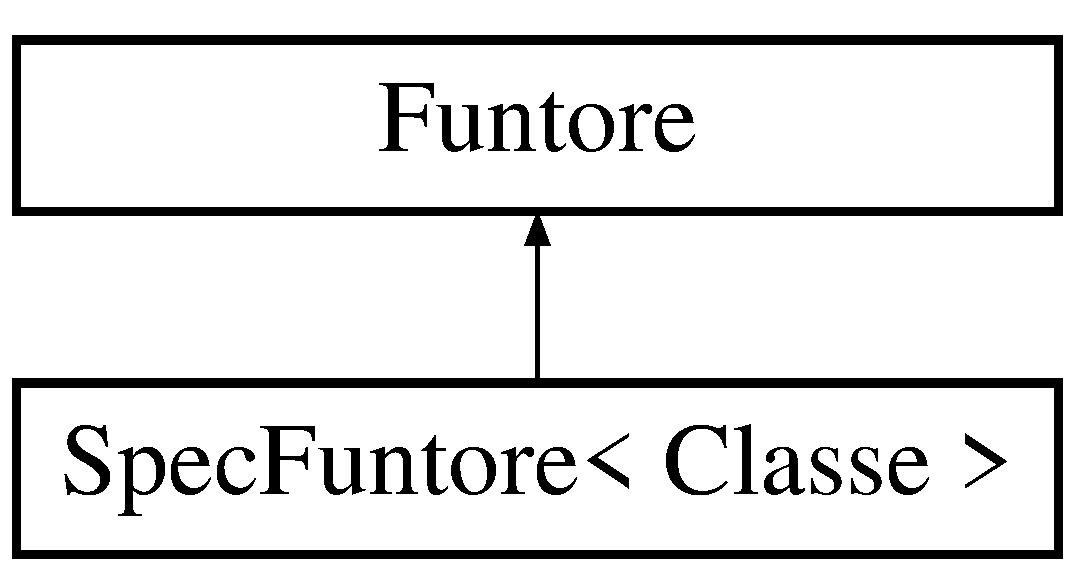
\includegraphics[height=2.000000cm]{classSpecFuntore}
\end{center}
\end{figure}
\subsubsection*{\-Public \-Member \-Functions}
\begin{DoxyCompactItemize}
\item 
\hypertarget{classSpecFuntore_aa876c38dd3e977523349978219f78810}{{\bfseries \-Spec\-Funtore} (\-Classe $\ast$\-\_\-pt2\-Object, void(\-Classe\-::$\ast$\-\_\-ftp)(double x))}\label{classSpecFuntore_aa876c38dd3e977523349978219f78810}

\item 
\hypertarget{classSpecFuntore_ad1b56a9087ec7ac49e01550c4db05cf9}{virtual double {\bfseries operator()} (const double x)}\label{classSpecFuntore_ad1b56a9087ec7ac49e01550c4db05cf9}

\item 
\hypertarget{classSpecFuntore_a38eee419ace8dfb106b346696cc54510}{virtual double {\bfseries \-Call} (double x)}\label{classSpecFuntore_a38eee419ace8dfb106b346696cc54510}

\end{DoxyCompactItemize}


\subsubsection{\-Detailed \-Description}
\subsubsection*{template$<$class Classe$>$class Spec\-Funtore$<$ Classe $>$}



\-Definition at line 345 of file \-Matematica.\-h.



\-The documentation for this class was generated from the following file\-:\begin{DoxyCompactItemize}
\item 
include/\-Matematica.\-h\end{DoxyCompactItemize}

\hypertarget{structSPLINE}{\subsection{\-S\-P\-L\-I\-N\-E \-Struct \-Reference}
\label{structSPLINE}\index{\-S\-P\-L\-I\-N\-E@{\-S\-P\-L\-I\-N\-E}}
}


\-Coefficient of a spline.  




{\ttfamily \#include $<$\-Matematica\-Struct.\-h$>$}

\subsubsection*{\-Public \-Attributes}
\begin{DoxyCompactItemize}
\item 
\hypertarget{structSPLINE_ad95dcba445836b4ba94129111a4b888c}{double \hyperlink{structSPLINE_ad95dcba445836b4ba94129111a4b888c}{a0}}\label{structSPLINE_ad95dcba445836b4ba94129111a4b888c}

\begin{DoxyCompactList}\small\item\em a0 + a1$\ast$x + a2$\ast$x$^\wedge$2 + a3$\ast$x$^\wedge$3 + a4$^\wedge$4 \end{DoxyCompactList}\item 
\hypertarget{structSPLINE_a5d015a3751aec61f2442b957cb6f517a}{double \hyperlink{structSPLINE_a5d015a3751aec61f2442b957cb6f517a}{a1}}\label{structSPLINE_a5d015a3751aec61f2442b957cb6f517a}

\begin{DoxyCompactList}\small\item\em a0 + a1$\ast$x + a2$\ast$x$^\wedge$2 + a3$\ast$x$^\wedge$3 + a4$^\wedge$4 \end{DoxyCompactList}\item 
\hypertarget{structSPLINE_ac55c2d269ed76bd9bdb7fb25f3533a4e}{double \hyperlink{structSPLINE_ac55c2d269ed76bd9bdb7fb25f3533a4e}{a2}}\label{structSPLINE_ac55c2d269ed76bd9bdb7fb25f3533a4e}

\begin{DoxyCompactList}\small\item\em a0 + a1$\ast$x + a2$\ast$x$^\wedge$2 + a3$\ast$x$^\wedge$3 + a4$^\wedge$4 \end{DoxyCompactList}\item 
\hypertarget{structSPLINE_aac922a785af4fb14fc828152cd94c34e}{double \hyperlink{structSPLINE_aac922a785af4fb14fc828152cd94c34e}{a3}}\label{structSPLINE_aac922a785af4fb14fc828152cd94c34e}

\begin{DoxyCompactList}\small\item\em a0 + a1$\ast$x + a2$\ast$x$^\wedge$2 + a3$\ast$x$^\wedge$3 + a4$^\wedge$4 \end{DoxyCompactList}\item 
\hypertarget{structSPLINE_ac6ef178808a2e015c97d93c99e52a441}{double \hyperlink{structSPLINE_ac6ef178808a2e015c97d93c99e52a441}{a4}}\label{structSPLINE_ac6ef178808a2e015c97d93c99e52a441}

\begin{DoxyCompactList}\small\item\em a0 + a1$\ast$x + a2$\ast$x$^\wedge$2 + a3$\ast$x$^\wedge$3 + a4$^\wedge$4 \end{DoxyCompactList}\end{DoxyCompactItemize}


\subsubsection{\-Detailed \-Description}
\-Coefficient of a spline. 

\-Definition at line 104 of file \-Matematica\-Struct.\-h.



\-The documentation for this struct was generated from the following file\-:\begin{DoxyCompactItemize}
\item 
include/\-Matematica\-Struct.\-h\end{DoxyCompactItemize}

\hypertarget{classSpline}{}\subsection{Spline Class Reference}
\label{classSpline}\index{Spline@{Spline}}


coeficients of a N order spline  


\subsubsection*{Public Member Functions}
\begin{DoxyCompactItemize}
\item 
\hyperlink{classSpline_afe6c93178a46d4e14c44c1d880c20c1b}{Spline} (int N)\hypertarget{classSpline_afe6c93178a46d4e14c44c1d880c20c1b}{}\label{classSpline_afe6c93178a46d4e14c44c1d880c20c1b}

\begin{DoxyCompactList}\small\item\em Allocate the memory. \end{DoxyCompactList}\item 
\hyperlink{classSpline_afe1affe99df46c8cce9f9853471f6e1b}{$\sim$\+Spline} ()\hypertarget{classSpline_afe1affe99df46c8cce9f9853471f6e1b}{}\label{classSpline_afe1affe99df46c8cce9f9853471f6e1b}

\begin{DoxyCompactList}\small\item\em Free the memory. \end{DoxyCompactList}\item 
int \hyperlink{classSpline_a265beffc4c9c8e21a31ae1af9f681f2a}{GetN} ()\hypertarget{classSpline_a265beffc4c9c8e21a31ae1af9f681f2a}{}\label{classSpline_a265beffc4c9c8e21a31ae1af9f681f2a}

\begin{DoxyCompactList}\small\item\em Print the number of coefficients. \end{DoxyCompactList}\item 
double \hyperlink{classSpline_aa2adff2f3dc7758073e3bcf79b67d678}{Get\+Coe} (int n)\hypertarget{classSpline_aa2adff2f3dc7758073e3bcf79b67d678}{}\label{classSpline_aa2adff2f3dc7758073e3bcf79b67d678}

\begin{DoxyCompactList}\small\item\em Print the n coefficient. \end{DoxyCompactList}\item 
void \hyperlink{classSpline_ae74ad20f1ff215326c2ef49911e605b1}{Set\+Coe} (double Val, int n)\hypertarget{classSpline_ae74ad20f1ff215326c2ef49911e605b1}{}\label{classSpline_ae74ad20f1ff215326c2ef49911e605b1}

\begin{DoxyCompactList}\small\item\em Set the n coefficient. \end{DoxyCompactList}\item 
void \hyperlink{classSpline_aeda17df26c0620cbf9e634c00de774df}{Add\+Coe} (double Val, int n)\hypertarget{classSpline_aeda17df26c0620cbf9e634c00de774df}{}\label{classSpline_aeda17df26c0620cbf9e634c00de774df}

\begin{DoxyCompactList}\small\item\em Add to the n coefficient. \end{DoxyCompactList}\end{DoxyCompactItemize}


\subsubsection{Detailed Description}
coeficients of a N order spline 

Definition at line 118 of file Matematica\+Struct.\+h.



The documentation for this class was generated from the following file\+:\begin{DoxyCompactItemize}
\item 
include/Matematica\+Struct.\+h\end{DoxyCompactItemize}

\hypertarget{structTENS}{}\subsection{T\+E\+NS Struct Reference}
\label{structTENS}\index{T\+E\+NS@{T\+E\+NS}}


Spatial tensor profile.  




{\ttfamily \#include $<$Forces.\+h$>$}

\subsubsection*{Public Attributes}
\begin{DoxyCompactItemize}
\item 
int \hyperlink{structTENS_a5a9396ca53c5306c34eb62ef4f02593b}{N\+Comp}\hypertarget{structTENS_a5a9396ca53c5306c34eb62ef4f02593b}{}\label{structTENS_a5a9396ca53c5306c34eb62ef4f02593b}

\begin{DoxyCompactList}\small\item\em \subsubsection*{of components}\end{DoxyCompactList}\item 
int \hyperlink{structTENS_a3b5e7568c0a268ec8bbeef7f29ea111a}{N\+Dim}\hypertarget{structTENS_a3b5e7568c0a268ec8bbeef7f29ea111a}{}\label{structTENS_a3b5e7568c0a268ec8bbeef7f29ea111a}

\begin{DoxyCompactList}\small\item\em \subsubsection*{of dimensions}\end{DoxyCompactList}\item 
int \hyperlink{structTENS_afa1c775c96b6e779b58ff0ff084d8cee}{N\+Slab}\hypertarget{structTENS_afa1c775c96b6e779b58ff0ff084d8cee}{}\label{structTENS_afa1c775c96b6e779b58ff0ff084d8cee}

\begin{DoxyCompactList}\small\item\em \subsubsection*{of slabs}\end{DoxyCompactList}\item 
int \hyperlink{structTENS_ae7fd260630480928a069e7e536739df1}{Calc\+Mode}\hypertarget{structTENS_ae7fd260630480928a069e7e536739df1}{}\label{structTENS_ae7fd260630480928a069e7e536739df1}

\begin{DoxyCompactList}\small\item\em Calculation mode. \end{DoxyCompactList}\item 
double $\ast$$\ast$ \hyperlink{structTENS_a3c45860d199670aae527e40339eb6437}{Pre}\hypertarget{structTENS_a3c45860d199670aae527e40339eb6437}{}\label{structTENS_a3c45860d199670aae527e40339eb6437}

\begin{DoxyCompactList}\small\item\em Pressure array. \end{DoxyCompactList}\item 
double $\ast$$\ast$ \hyperlink{structTENS_a0041877aa9f9820a1c0506e9aa9403c3}{Dens}\hypertarget{structTENS_a0041877aa9f9820a1c0506e9aa9403c3}{}\label{structTENS_a0041877aa9f9820a1c0506e9aa9403c3}

\begin{DoxyCompactList}\small\item\em Density array. \end{DoxyCompactList}\item 
double \hyperlink{structTENS_a7a515f1ba73761bc36f223dd97aed95f}{Pre\+Tot} \mbox{[}3\mbox{]}\hypertarget{structTENS_a7a515f1ba73761bc36f223dd97aed95f}{}\label{structTENS_a7a515f1ba73761bc36f223dd97aed95f}

\begin{DoxyCompactList}\small\item\em Total pressure. \end{DoxyCompactList}\item 
double \hyperlink{structTENS_a9fce28b2676fbd55604124a7ee638964}{Ref\+Pos} \mbox{[}3\mbox{]}\hypertarget{structTENS_a9fce28b2676fbd55604124a7ee638964}{}\label{structTENS_a9fce28b2676fbd55604124a7ee638964}

\begin{DoxyCompactList}\small\item\em Reference point. \end{DoxyCompactList}\item 
double \hyperlink{structTENS_a8895c89605e91c6cf7430bad336f77c6}{Edge} \mbox{[}3\mbox{]}\hypertarget{structTENS_a8895c89605e91c6cf7430bad336f77c6}{}\label{structTENS_a8895c89605e91c6cf7430bad336f77c6}

\begin{DoxyCompactList}\small\item\em Edges. \end{DoxyCompactList}\item 
int \hyperlink{structTENS_af7ac0af936a90fda61fc97028cc7a2fc}{Wrap} \mbox{[}3\mbox{]}\hypertarget{structTENS_af7ac0af936a90fda61fc97028cc7a2fc}{}\label{structTENS_af7ac0af936a90fda61fc97028cc7a2fc}

\begin{DoxyCompactList}\small\item\em Which coordinate to wrap. \end{DoxyCompactList}\item 
double \hyperlink{structTENS_a8deae0979f1ffa0ff0b1976cee071f39}{Edge\+Inv} \mbox{[}3\mbox{]}\hypertarget{structTENS_a8deae0979f1ffa0ff0b1976cee071f39}{}\label{structTENS_a8deae0979f1ffa0ff0b1976cee071f39}

\begin{DoxyCompactList}\small\item\em Inverse of the edges. \end{DoxyCompactList}\end{DoxyCompactItemize}


\subsubsection{Detailed Description}
Spatial tensor profile. 

Definition at line 189 of file Forces.\+h.



The documentation for this struct was generated from the following file\+:\begin{DoxyCompactItemize}
\item 
src/\+Addyn/Forces.\+h\end{DoxyCompactItemize}

\hypertarget{structVAR__LINE}{\subsection{\-V\-A\-R\-\_\-\-L\-I\-N\-E \-Struct \-Reference}
\label{structVAR__LINE}\index{\-V\-A\-R\-\_\-\-L\-I\-N\-E@{\-V\-A\-R\-\_\-\-L\-I\-N\-E}}
}


\-Define a triangle.  




{\ttfamily \#include $<$\-Var\-Data.\-h$>$}

\subsubsection*{\-Public \-Attributes}
\begin{DoxyCompactItemize}
\item 
\hypertarget{structVAR__LINE_a411315336ef1ae37448e44ee3cc83503}{\hyperlink{structXYZ}{\-X\-Y\-Z} \hyperlink{structVAR__LINE_a411315336ef1ae37448e44ee3cc83503}{p} \mbox{[}2\mbox{]}}\label{structVAR__LINE_a411315336ef1ae37448e44ee3cc83503}

\begin{DoxyCompactList}\small\item\em \-The two vertices. \end{DoxyCompactList}\item 
\hypertarget{structVAR__LINE_ae93aa7b3bc74295f6f1118a6b0a0e804}{\hyperlink{structXYZ}{\-X\-Y\-Z} \hyperlink{structVAR__LINE_ae93aa7b3bc74295f6f1118a6b0a0e804}{c}}\label{structVAR__LINE_ae93aa7b3bc74295f6f1118a6b0a0e804}

\begin{DoxyCompactList}\small\item\em \-Centroid. \end{DoxyCompactList}\item 
\hypertarget{structVAR__LINE_aa8fc460cb352395b8303f6bd1f49c9ad}{int \hyperlink{structVAR__LINE_aa8fc460cb352395b8303f6bd1f49c9ad}{v} \mbox{[}2\mbox{]}}\label{structVAR__LINE_aa8fc460cb352395b8303f6bd1f49c9ad}

\begin{DoxyCompactList}\small\item\em \-Reference for the vectors. \end{DoxyCompactList}\item 
\hypertarget{structVAR__LINE_a5da38476370426c07250979c5c998715}{\hyperlink{structXYZ}{\-X\-Y\-Z} \hyperlink{structVAR__LINE_a5da38476370426c07250979c5c998715}{n} \mbox{[}2\mbox{]}}\label{structVAR__LINE_a5da38476370426c07250979c5c998715}

\begin{DoxyCompactList}\small\item\em \-Normal to the vertices. \end{DoxyCompactList}\end{DoxyCompactItemize}


\subsubsection{\-Detailed \-Description}
\-Define a triangle. 

\-Definition at line 509 of file \-Var\-Data.\-h.



\-The documentation for this struct was generated from the following file\-:\begin{DoxyCompactItemize}
\item 
include/\-Var\-Data.\-h\end{DoxyCompactItemize}

\hypertarget{structVAR__TRIANGLE}{\subsection{\-V\-A\-R\-\_\-\-T\-R\-I\-A\-N\-G\-L\-E \-Struct \-Reference}
\label{structVAR__TRIANGLE}\index{\-V\-A\-R\-\_\-\-T\-R\-I\-A\-N\-G\-L\-E@{\-V\-A\-R\-\_\-\-T\-R\-I\-A\-N\-G\-L\-E}}
}


\-Define a triangle.  




{\ttfamily \#include $<$\-Var\-Data.\-h$>$}

\subsubsection*{\-Public \-Attributes}
\begin{DoxyCompactItemize}
\item 
\hypertarget{structVAR__TRIANGLE_abb19475a6b83f96d1f41b2a120910022}{\hyperlink{structXYZ}{\-X\-Y\-Z} \hyperlink{structVAR__TRIANGLE_abb19475a6b83f96d1f41b2a120910022}{p} \mbox{[}3\mbox{]}}\label{structVAR__TRIANGLE_abb19475a6b83f96d1f41b2a120910022}

\begin{DoxyCompactList}\small\item\em \-The three vertices. \end{DoxyCompactList}\item 
\hypertarget{structVAR__TRIANGLE_ae93aa7b3bc74295f6f1118a6b0a0e804}{\hyperlink{structXYZ}{\-X\-Y\-Z} \hyperlink{structVAR__TRIANGLE_ae93aa7b3bc74295f6f1118a6b0a0e804}{c}}\label{structVAR__TRIANGLE_ae93aa7b3bc74295f6f1118a6b0a0e804}

\begin{DoxyCompactList}\small\item\em \-Centroid. \end{DoxyCompactList}\item 
\hypertarget{structVAR__TRIANGLE_adf75f0e81beb91b0ef5de318ab595455}{int \hyperlink{structVAR__TRIANGLE_adf75f0e81beb91b0ef5de318ab595455}{v} \mbox{[}3\mbox{]}}\label{structVAR__TRIANGLE_adf75f0e81beb91b0ef5de318ab595455}

\begin{DoxyCompactList}\small\item\em \-Reference for the vectors. \end{DoxyCompactList}\item 
\hypertarget{structVAR__TRIANGLE_a1db8f1be3299f0c5f218cf0142c6c687}{\hyperlink{structXYZ}{\-X\-Y\-Z} \hyperlink{structVAR__TRIANGLE_a1db8f1be3299f0c5f218cf0142c6c687}{n} \mbox{[}3\mbox{]}}\label{structVAR__TRIANGLE_a1db8f1be3299f0c5f218cf0142c6c687}

\begin{DoxyCompactList}\small\item\em \-Normal to the vertices. \end{DoxyCompactList}\end{DoxyCompactItemize}


\subsubsection{\-Detailed \-Description}
\-Define a triangle. 

\-Definition at line 498 of file \-Var\-Data.\-h.



\-The documentation for this struct was generated from the following file\-:\begin{DoxyCompactItemize}
\item 
include/\-Var\-Data.\-h\end{DoxyCompactItemize}

\hypertarget{classVarData}{\subsection{\-Var\-Data \-Class \-Reference}
\label{classVarData}\index{\-Var\-Data@{\-Var\-Data}}
}


\-Reads and elaborates a system of chains.  




{\ttfamily \#include $<$\-Var\-Data.\-h$>$}

\-Inheritance diagram for \-Var\-Data\-:\begin{figure}[H]
\begin{center}
\leavevmode
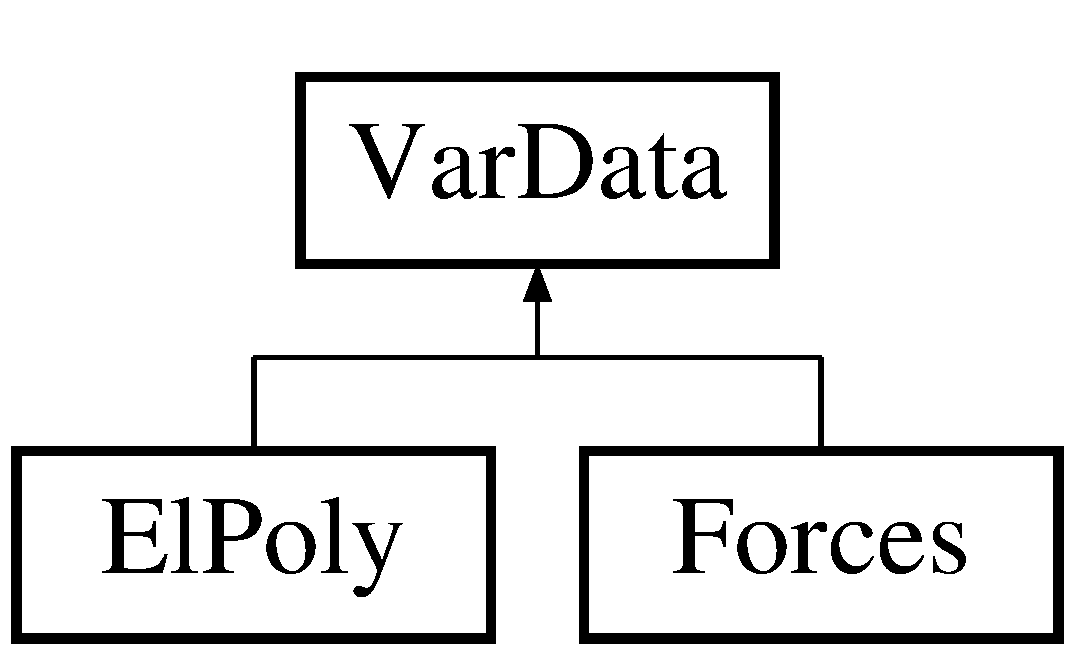
\includegraphics[height=2.000000cm]{classVarData}
\end{center}
\end{figure}
\subsubsection*{\-Public \-Types}
\begin{DoxyCompactItemize}
\item 
\hypertarget{classVarData_aea7b2bfbbf53c129db630b86e42af630}{typedef double(\-Var\-Data\-::$\ast$ \hyperlink{classVarData_aea7b2bfbbf53c129db630b86e42af630}{\-N\-A\-N\-O\-\_\-\-D\-I\-S\-T} )(double $\ast$\-Pos, int n)}\label{classVarData_aea7b2bfbbf53c129db630b86e42af630}

\begin{DoxyCompactList}\small\item\em \-Data type for distance/field functions. \end{DoxyCompactList}\end{DoxyCompactItemize}
\subsubsection*{\-Public \-Member \-Functions}
\begin{DoxyCompactItemize}
\item 
\hypertarget{classVarData_a159e408a7c67c4b4ff12edd72d315bd4}{\hyperlink{classVarData_a159e408a7c67c4b4ff12edd72d315bd4}{\-Var\-Data} ()}\label{classVarData_a159e408a7c67c4b4ff12edd72d315bd4}

\begin{DoxyCompactList}\small\item\em \-Set the constants. \end{DoxyCompactList}\item 
\hypertarget{classVarData_a66a331d8378209908c6b154d79723977}{\hyperlink{classVarData_a66a331d8378209908c6b154d79723977}{$\sim$\-Var\-Data} ()}\label{classVarData_a66a331d8378209908c6b154d79723977}

\begin{DoxyCompactList}\small\item\em \-Destructor. \end{DoxyCompactList}\item 
\hypertarget{classVarData_a616b8e0974fde7798bb09b9af1b339ae}{void \hyperlink{classVarData_a616b8e0974fde7798bb09b9af1b339ae}{\-Var\-Message} (const char $\ast$s,...)}\label{classVarData_a616b8e0974fde7798bb09b9af1b339ae}

\begin{DoxyCompactList}\small\item\em \-If enabled call the function position. \end{DoxyCompactList}\item 
bool \hyperlink{classVarData_a50a785f6295f7e7fb2494fcad2a2a7fc}{\-Open} (char $\ast$\-In\-File, int \-B\-F)
\begin{DoxyCompactList}\small\item\em \-Open the. \end{DoxyCompactList}\item 
\hypertarget{classVarData_a385ea4b67d94de234204940ef8da368d}{bool \hyperlink{classVarData_a385ea4b67d94de234204940ef8da368d}{\-Open\-Risk} (char $\ast$\-In\-File, int \-B\-F)}\label{classVarData_a385ea4b67d94de234204940ef8da368d}

\begin{DoxyCompactList}\small\item\em \-Opens a file without reallocationg. \end{DoxyCompactList}\item 
\hypertarget{classVarData_a2d7ca8dfc2fc40c902e22b3110f359ca}{bool \hyperlink{classVarData_a2d7ca8dfc2fc40c902e22b3110f359ca}{\-Open\-Trust} (char $\ast$\-In\-File, int \-B\-F)}\label{classVarData_a2d7ca8dfc2fc40c902e22b3110f359ca}

\begin{DoxyCompactList}\small\item\em \-Opens a file checking if the information are correct. \end{DoxyCompactList}\item 
\hypertarget{classVarData_a1a9b1fc0b7f08d25f507becdb57d531e}{void \hyperlink{classVarData_a1a9b1fc0b7f08d25f507becdb57d531e}{\-Alloc\-Part} ()}\label{classVarData_a1a9b1fc0b7f08d25f507becdb57d531e}

\begin{DoxyCompactList}\small\item\em \-Alloc the structures. \end{DoxyCompactList}\item 
\hypertarget{classVarData_ab725e5f5e1306bb770cffc9171abbf95}{void \hyperlink{classVarData_ab725e5f5e1306bb770cffc9171abbf95}{\-Alloc\-Chain} ()}\label{classVarData_ab725e5f5e1306bb770cffc9171abbf95}

\begin{DoxyCompactList}\small\item\em \-Alloc the structures. \end{DoxyCompactList}\item 
\hypertarget{classVarData_a5440abb543ae3c83d1b628b0ba0eb3c6}{\hyperlink{classProperties}{\-Properties} \hyperlink{classVarData_a5440abb543ae3c83d1b628b0ba0eb3c6}{\-Sys\-Properties} ()}\label{classVarData_a5440abb543ae3c83d1b628b0ba0eb3c6}

\begin{DoxyCompactList}\small\item\em \-Calculate some basis properties. \end{DoxyCompactList}\item 
\hypertarget{classVarData_a4dd85f1789027793b97a591acc9caf30}{void \hyperlink{classVarData_a4dd85f1789027793b97a591acc9caf30}{\-Sys\-Info} (char $\ast$c\-System)}\label{classVarData_a4dd85f1789027793b97a591acc9caf30}

\begin{DoxyCompactList}\small\item\em \-Print a string with the system information. \end{DoxyCompactList}\item 
\hypertarget{classVarData_aa415b42b89dfba2ab8189be4e86b41ad}{void \hyperlink{classVarData_aa415b42b89dfba2ab8189be4e86b41ad}{\-Sys\-Def} (char $\ast$c\-System)}\label{classVarData_aa415b42b89dfba2ab8189be4e86b41ad}

\begin{DoxyCompactList}\small\item\em \-Print a string with the system definitions. \end{DoxyCompactList}\item 
\hypertarget{classVarData_a497026b20d4baf7d7812310a50a73154}{char $\ast$ \hyperlink{classVarData_a497026b20d4baf7d7812310a50a73154}{\-Sys\-State} ()}\label{classVarData_a497026b20d4baf7d7812310a50a73154}

\begin{DoxyCompactList}\small\item\em \-Calculates fundamental quantities. \end{DoxyCompactList}\item 
\hypertarget{classVarData_a5dd46e77250756dc756a8a5aae0b575f}{void \hyperlink{classVarData_a5dd46e77250756dc756a8a5aae0b575f}{\-Set\-Coeff} ()}\label{classVarData_a5dd46e77250756dc756a8a5aae0b575f}

\begin{DoxyCompactList}\small\item\em \-Set the virial coefficients from the known values of density coex... \end{DoxyCompactList}\item 
\hypertarget{classVarData_a8e4611ad8a334d8a27c2fb87e7ea0df1}{void \hyperlink{classVarData_a8e4611ad8a334d8a27c2fb87e7ea0df1}{\-Set\-Coeff} (double $\ast$v2, double $\ast$v3)}\label{classVarData_a8e4611ad8a334d8a27c2fb87e7ea0df1}

\begin{DoxyCompactList}\small\item\em \-Set and normalize the virial coefficients from the arrays v2 and v3. \end{DoxyCompactList}\item 
\hypertarget{classVarData_a19886baf2914ac46bc50f333254a4e57}{double \hyperlink{classVarData_a19886baf2914ac46bc50f333254a4e57}{\-Two\-Part\-Dist} (int p1, int p2, double $\ast$\-Rel\-Dist)}\label{classVarData_a19886baf2914ac46bc50f333254a4e57}

\begin{DoxyCompactList}\small\item\em \-Return the relative distance between two particles (wrapped) \end{DoxyCompactList}\item 
\hypertarget{classVarData_a118d59dbacc06ea6d6b4f8e2cf864406}{double \hyperlink{classVarData_a118d59dbacc06ea6d6b4f8e2cf864406}{\-Two\-Part\-Dist} (double $\ast$\-Pos, int p2, double $\ast$\-Rel\-Dist)}\label{classVarData_a118d59dbacc06ea6d6b4f8e2cf864406}

\begin{DoxyCompactList}\small\item\em \-Return the relative distance between two particles (wrapped) \end{DoxyCompactList}\item 
\hypertarget{classVarData_a8c36154f85dd7e41560448d01aab695d}{double \hyperlink{classVarData_a8c36154f85dd7e41560448d01aab695d}{\-Two\-Part\-Dist2} (int p1, int p2, double $\ast$\-Rel\-Dist)}\label{classVarData_a8c36154f85dd7e41560448d01aab695d}

\begin{DoxyCompactList}\small\item\em \-Return the relative distance between two particles (wrapped) \end{DoxyCompactList}\item 
\hypertarget{classVarData_ac18654b4b07d2480609388a671319d76}{double \hyperlink{classVarData_ac18654b4b07d2480609388a671319d76}{\-Two\-Part\-Dist2} (double $\ast$\-Pos, int p2, double $\ast$\-Rel\-Dist)}\label{classVarData_ac18654b4b07d2480609388a671319d76}

\begin{DoxyCompactList}\small\item\em \-Return the relative distance between two particles (wrapped) \end{DoxyCompactList}\item 
\hypertarget{classVarData_a72b2b49ea5c00c2902e419ff8ec9a095}{int \hyperlink{classVarData_a72b2b49ea5c00c2902e419ff8ec9a095}{\-Two\-Part\-Dist} (int p1, int p2, double $\ast$\-Rel\-Dist, double \-Cut\-Off)}\label{classVarData_a72b2b49ea5c00c2902e419ff8ec9a095}

\begin{DoxyCompactList}\small\item\em \-Return the relative distance between two particles (wrapped) if the particles are within the cut off. \end{DoxyCompactList}\item 
\hypertarget{classVarData_a7ecd9d43c45ae675e71f9b926673c8e4}{int \hyperlink{classVarData_a7ecd9d43c45ae675e71f9b926673c8e4}{\-Two\-Part\-Dist} (double $\ast$\-Pos, int p2, double $\ast$\-Rel\-Dist, double \-Cut\-Off)}\label{classVarData_a7ecd9d43c45ae675e71f9b926673c8e4}

\begin{DoxyCompactList}\small\item\em \-Return the relative distance between two particles (wrapped) if the particles are within the cut off. \end{DoxyCompactList}\item 
\hypertarget{classVarData_a054aab836dcf7735720ef32e0b8f7ecb}{bool \hyperlink{classVarData_a054aab836dcf7735720ef32e0b8f7ecb}{\-Write} (char $\ast$\-Out\-File)}\label{classVarData_a054aab836dcf7735720ef32e0b8f7ecb}

\begin{DoxyCompactList}\small\item\em \-Writes a \char`\"{}system-\/file\char`\"{} or a \char`\"{}x y z\char`\"{} file". \end{DoxyCompactList}\item 
\hypertarget{classVarData_a76873542f36c8e36b790c90273c95cf1}{bool \hyperlink{classVarData_a76873542f36c8e36b790c90273c95cf1}{\-Write\-Txvl} (char $\ast$\-Out\-File)}\label{classVarData_a76873542f36c8e36b790c90273c95cf1}

\begin{DoxyCompactList}\small\item\em \-Writes a \char`\"{}system-\/file\char`\"{} or a \char`\"{}x y z\char`\"{} file". \end{DoxyCompactList}\item 
\hypertarget{classVarData_a4bed1297ee4f1c6966e1f8389e3b34c8}{bool \hyperlink{classVarData_a4bed1297ee4f1c6966e1f8389e3b34c8}{\-Write\-Xvt} (char $\ast$\-Out\-File)}\label{classVarData_a4bed1297ee4f1c6966e1f8389e3b34c8}

\begin{DoxyCompactList}\small\item\em \-Writes a \char`\"{}system-\/file\char`\"{} or a \char`\"{}x y z\char`\"{} file". \end{DoxyCompactList}\item 
\hypertarget{classVarData_a842c747bebda7f52b905605b1446c814}{bool \hyperlink{classVarData_a842c747bebda7f52b905605b1446c814}{\-Write\-Xyz} (char $\ast$\-Out\-File)}\label{classVarData_a842c747bebda7f52b905605b1446c814}

\begin{DoxyCompactList}\small\item\em \-Writes a \char`\"{}system-\/file\char`\"{} or a \char`\"{}x y z\char`\"{} file". \end{DoxyCompactList}\item 
\hypertarget{classVarData_a4a4c970350675e5a82a935c754264d14}{void \hyperlink{classVarData_a4a4c970350675e5a82a935c754264d14}{\-Header\-Interaction} (\-F\-I\-L\-E $\ast$\-File\-To\-Write)}\label{classVarData_a4a4c970350675e5a82a935c754264d14}

\begin{DoxyCompactList}\small\item\em \-Header interactions. \end{DoxyCompactList}\item 
\hypertarget{classVarData_ab0cc3088657341d2696949515927e91c}{void \hyperlink{classVarData_ab0cc3088657341d2696949515927e91c}{\-String\-Nano} (char $\ast$\-N\-String, int n)}\label{classVarData_ab0cc3088657341d2696949515927e91c}

\begin{DoxyCompactList}\small\item\em \-String for the rigid inclusion in the header file. \end{DoxyCompactList}\item 
\hypertarget{classVarData_af86d3fd2dc311c093cd03f65eb3fadd9}{int \hyperlink{classVarData_af86d3fd2dc311c093cd03f65eb3fadd9}{\-Header\-Nano} (\-F\-I\-L\-E $\ast$\-File\-To\-Write)}\label{classVarData_af86d3fd2dc311c093cd03f65eb3fadd9}

\begin{DoxyCompactList}\small\item\em \-Write the nano section of the header to the file. \end{DoxyCompactList}\item 
\hypertarget{classVarData_ad86f36df8d1ff2f5c4e8f9bf3e43dfa3}{int \hyperlink{classVarData_ad86f36df8d1ff2f5c4e8f9bf3e43dfa3}{\-Header\-Soft} (char $\ast$\-Line)}\label{classVarData_ad86f36df8d1ff2f5c4e8f9bf3e43dfa3}

\begin{DoxyCompactList}\small\item\em \-Header soft. \end{DoxyCompactList}\item 
\hypertarget{classVarData_afaf46d635173dcc718ad3eb8870d4b91}{void \hyperlink{classVarData_afaf46d635173dcc718ad3eb8870d4b91}{\-Write\-Linked\-Surf} (\-F\-I\-L\-E $\ast$\-F\-Write, double $\ast$\-Plot, int \-N\-Sample, int \-N\-Type, double $\ast$\-Bound, int $\ast$\-P\-Id)}\label{classVarData_afaf46d635173dcc718ad3eb8870d4b91}

\begin{DoxyCompactList}\small\item\em \-Write the positions of the egdes of the rectangles. \end{DoxyCompactList}\item 
\hypertarget{classVarData_a05977dbae3f034b4371646d6c1afbdcd}{void \hyperlink{classVarData_a05977dbae3f034b4371646d6c1afbdcd}{\-Write\-Surf} (\-F\-I\-L\-E $\ast$\-F2\-Write, double $\ast$$\ast$\-Plot, int \-N\-Sample, int \-Off\-Set)}\label{classVarData_a05977dbae3f034b4371646d6c1afbdcd}

\begin{DoxyCompactList}\small\item\em \-Write the particle position as linked edges of squares. \end{DoxyCompactList}\item 
\hypertarget{classVarData_a3043b04de19ff9f50f6253ecbdf316bd}{void \hyperlink{classVarData_a3043b04de19ff9f50f6253ecbdf316bd}{\-Shape\-Id} (int i\-Shape, char $\ast$\-Shape)}\label{classVarData_a3043b04de19ff9f50f6253ecbdf316bd}

\begin{DoxyCompactList}\small\item\em \-Identifier of the shape. \end{DoxyCompactList}\item 
\hypertarget{classVarData_a76c0ae2bedaaafb3da1cb7019035b602}{bool \hyperlink{classVarData_a76c0ae2bedaaafb3da1cb7019035b602}{\-Back\-Fold} (int \-How)}\label{classVarData_a76c0ae2bedaaafb3da1cb7019035b602}

\begin{DoxyCompactList}\small\item\em \-Backfold the particle position. \end{DoxyCompactList}\item 
\hypertarget{classVarData_a0826d64fb693577d667b53d50e53abb5}{int \hyperlink{classVarData_a0826d64fb693577d667b53d50e53abb5}{\-Bf\-Def\-Chain} ()}\label{classVarData_a0826d64fb693577d667b53d50e53abb5}

\begin{DoxyCompactList}\small\item\em \-Definition of the chain. \end{DoxyCompactList}\item 
\hypertarget{classVarData_af16fce4f3d2abd5981a02ce3a9bf0ee3}{int \hyperlink{classVarData_af16fce4f3d2abd5981a02ce3a9bf0ee3}{\-Bf\-Edge} ()}\label{classVarData_af16fce4f3d2abd5981a02ce3a9bf0ee3}

\begin{DoxyCompactList}\small\item\em \-Find the box size if missing. \end{DoxyCompactList}\item 
\hypertarget{classVarData_ae1ce909c47c5e9f7aa655b443dd74af0}{void \hyperlink{classVarData_ae1ce909c47c5e9f7aa655b443dd74af0}{\-Dist\-From\-Np} ()}\label{classVarData_ae1ce909c47c5e9f7aa655b443dd74af0}

\begin{DoxyCompactList}\small\item\em \-Define the distance form the nanoparticle. \end{DoxyCompactList}\item 
\hypertarget{classVarData_a42c97b08cf848bfaa9d68951070243d2}{void \hyperlink{classVarData_a42c97b08cf848bfaa9d68951070243d2}{\-Shift\-Ref} (int \hyperlink{classVarData_a76c0ae2bedaaafb3da1cb7019035b602}{\-Back\-Fold})}\label{classVarData_a42c97b08cf848bfaa9d68951070243d2}

\begin{DoxyCompactList}\small\item\em \-Backfold the system wrt the reference position. \end{DoxyCompactList}\item 
\hypertarget{classVarData_a368f70b601610ec1c3b3155e681cfa83}{int \hyperlink{classVarData_a368f70b601610ec1c3b3155e681cfa83}{\-Stalk\-Pos} (double $\ast$\-Old\-Pos)}\label{classVarData_a368f70b601610ec1c3b3155e681cfa83}

\begin{DoxyCompactList}\small\item\em \-Find the position of the stalk. \end{DoxyCompactList}\item 
\hypertarget{classVarData_a71d64d583aa288c4bc45579df741ea07}{void \hyperlink{classVarData_a71d64d583aa288c4bc45579df741ea07}{\-Bf\-Pep} ()}\label{classVarData_a71d64d583aa288c4bc45579df741ea07}

\begin{DoxyCompactList}\small\item\em \-Backfold the nano described as a cluster of monomers. \end{DoxyCompactList}\item 
\hypertarget{classVarData_abe9b658d50575d5d6be580bc87f3b4ac}{void \hyperlink{classVarData_abe9b658d50575d5d6be580bc87f3b4ac}{\-Back\-Bone} (double $\ast$\-Line, int \-N\-Bin)}\label{classVarData_abe9b658d50575d5d6be580bc87f3b4ac}

\begin{DoxyCompactList}\small\item\em \-Describe the backbone of a filament. \end{DoxyCompactList}\item 
\hypertarget{classVarData_af1b41051cede003baf90d8a7bf49ca8d}{void \hyperlink{classVarData_af1b41051cede003baf90d8a7bf49ca8d}{\-Stalk\-Line\-Prof} (double $\ast$\-Line, int \-N\-Bin)}\label{classVarData_af1b41051cede003baf90d8a7bf49ca8d}

\begin{DoxyCompactList}\small\item\em \-Describe the line for a linear stalk. \end{DoxyCompactList}\item 
\hypertarget{classVarData_a27d73648f0e3e381a832e8e9002a3bd6}{void \hyperlink{classVarData_a27d73648f0e3e381a832e8e9002a3bd6}{\-Stalk\-Pos2} (double $\ast$\-Old\-Pos, double $\ast$\-Cm\-Stalk)}\label{classVarData_a27d73648f0e3e381a832e8e9002a3bd6}

\begin{DoxyCompactList}\small\item\em \-Find the position of the stalk second method. \end{DoxyCompactList}\item 
\hypertarget{classVarData_aa2acae864359003a4b752ed363262f14}{void \hyperlink{classVarData_aa2acae864359003a4b752ed363262f14}{\-Stalk\-Pos3} (double $\ast$\-Old\-Pos, double $\ast$\-Cm\-Stalk)}\label{classVarData_aa2acae864359003a4b752ed363262f14}

\begin{DoxyCompactList}\small\item\em \-Find the position of the stalk third method. \end{DoxyCompactList}\item 
\hypertarget{classVarData_a57ab5d38a7d7936277859f39a525edb4}{int \hyperlink{classVarData_a57ab5d38a7d7936277859f39a525edb4}{\-Stalk\-Pos4} (double $\ast$\-Old\-Pos, double $\ast$\-Cm\-Stalk)}\label{classVarData_a57ab5d38a7d7936277859f39a525edb4}

\begin{DoxyCompactList}\small\item\em \-Find the position of the stalk forth method. \end{DoxyCompactList}\item 
\hypertarget{classVarData_a4af146ff5f41159dbc594bf50a1b1820}{double \hyperlink{classVarData_a4af146ff5f41159dbc594bf50a1b1820}{\-Normal\-Weight} (\hyperlink{structVAR__TRIANGLE}{\-V\-A\-R\-\_\-\-T\-R\-I\-A\-N\-G\-L\-E} $\ast$\-Triang, double $\ast$\-Weight, int \-N\-Grid, int \-N\-Tri)}\label{classVarData_a4af146ff5f41159dbc594bf50a1b1820}

\begin{DoxyCompactList}\small\item\em \-Weight of the neighblorung normal on a vertex. \end{DoxyCompactList}\item 
void \hyperlink{classVarData_abeac0d2b6f91beee12e2506a41eca70c}{\-Connect\-Line\-Chain} (\hyperlink{structVAR__LINE}{\-V\-A\-R\-\_\-\-L\-I\-N\-E} $\ast$\-Triang, int \-N\-Grid, int \-N\-Tri)
\begin{DoxyCompactList}\small\item\em \-Connect the lines in a chain. \end{DoxyCompactList}\item 
void \hyperlink{classVarData_a2e9b9e5912554bc52210356f6e2b1bc8}{\-Connect\-Line\-Chain2} (\hyperlink{structVAR__LINE}{\-V\-A\-R\-\_\-\-L\-I\-N\-E} $\ast$\-Triang, int \-N\-Grid, int \-N\-Tri)
\begin{DoxyCompactList}\small\item\em \-Connect the lines in a chain. \end{DoxyCompactList}\item 
void \hyperlink{classVarData_a1f3c69ce2b4b130fead4373fa76700f3}{\-Connect\-Line\-Chain3} (\hyperlink{structVAR__LINE}{\-V\-A\-R\-\_\-\-L\-I\-N\-E} $\ast$\-Triang, int \-N\-Grid, int \-N\-Tri)
\begin{DoxyCompactList}\small\item\em \-Connect the lines in a chain. \end{DoxyCompactList}\item 
\hypertarget{classVarData_a90139ee28a0c75803648d2b1d85e80ce}{double \hyperlink{classVarData_a90139ee28a0c75803648d2b1d85e80ce}{\-Pore\-Pos} ()}\label{classVarData_a90139ee28a0c75803648d2b1d85e80ce}

\begin{DoxyCompactList}\small\item\em \-Find the position of the pore. \end{DoxyCompactList}\item 
\hypertarget{classVarData_a795f774737c0deac9dfac3edb068526e}{int \hyperlink{classVarData_a795f774737c0deac9dfac3edb068526e}{\-Fetch} (char $\ast$str, char $\ast$mask, char $\ast$fmt,...)}\label{classVarData_a795f774737c0deac9dfac3edb068526e}

\begin{DoxyCompactList}\small\item\em \-Retrive from a string the information concerning the mask. \end{DoxyCompactList}\item 
\hypertarget{classVarData_a57563378ffd76c20068f612fbec29e3d}{int \hyperlink{classVarData_a57563378ffd76c20068f612fbec29e3d}{\-Braket\-Pos} (char $\ast$str, char $\ast$mask, int $\ast$s\-Pos, int $\ast$s\-Len)}\label{classVarData_a57563378ffd76c20068f612fbec29e3d}

\begin{DoxyCompactList}\small\item\em \-Retrive from a string the position of the brakets. \end{DoxyCompactList}\item 
\hypertarget{classVarData_a05ab100c879ea5377012188f65db69b1}{int \hyperlink{classVarData_a05ab100c879ea5377012188f65db69b1}{\-Fetch} (char $\ast$str, char $\ast$mask, int \-N\-Arg, double $\ast$\-Val)}\label{classVarData_a05ab100c879ea5377012188f65db69b1}

\begin{DoxyCompactList}\small\item\em \-Retrive from a string the information concerning the mask. \end{DoxyCompactList}\item 
bool \hyperlink{classVarData_ab48c8e53b923767c73cb13848ecd2fd6}{\-Read\-String} (const char $\ast$\-String, char $\ast$c\-Line, double $\ast$\-Value)
\begin{DoxyCompactList}\small\item\em \-Copy the value in the. \end{DoxyCompactList}\item 
bool \hyperlink{classVarData_a337c48b3218d18409ff180f710421f2d}{\-Read\-String} (const char $\ast$\-String, double $\ast$\-Value, char $\ast$line)
\begin{DoxyCompactList}\small\item\em \-Copy the value in the. \end{DoxyCompactList}\item 
bool \hyperlink{classVarData_adaef8865e533156a71becc0fa083eb9b}{\-Read\-String} (const char $\ast$\-String, char $\ast$c\-Line, int $\ast$\-Value)
\begin{DoxyCompactList}\small\item\em \-Copy the value in the. \end{DoxyCompactList}\item 
\hypertarget{classVarData_a91210b2064dbd96a76aeeadf9a3d3364}{int \hyperlink{classVarData_a91210b2064dbd96a76aeeadf9a3d3364}{\-Read\-Val} (char $\ast$p\-Line, double $\ast$\-Value)}\label{classVarData_a91210b2064dbd96a76aeeadf9a3d3364}

\begin{DoxyCompactList}\small\item\em \-Copy the value in the \-String to the \-Value referring to the position of p\-Line. \end{DoxyCompactList}\item 
\hypertarget{classVarData_aa7f1d8e6b048273ed4b7fc4b653427d0}{int \hyperlink{classVarData_aa7f1d8e6b048273ed4b7fc4b653427d0}{\-Read\-Line\-Xvt} (char $\ast$c\-Line, double $\ast$\-Pos, int $\ast$\-Type)}\label{classVarData_aa7f1d8e6b048273ed4b7fc4b653427d0}

\begin{DoxyCompactList}\small\item\em \-Read a single line in format \-Xvt. \end{DoxyCompactList}\item 
\hypertarget{classVarData_a36c85650c83c9e9e2c97b29ebbf4e782}{bool \hyperlink{classVarData_a36c85650c83c9e9e2c97b29ebbf4e782}{\-Read\-Conf} (char $\ast$\-In\-File)}\label{classVarData_a36c85650c83c9e9e2c97b29ebbf4e782}

\begin{DoxyCompactList}\small\item\em \-Reads a \char`\"{}configuration file\char`\"{}. \end{DoxyCompactList}\item 
\hypertarget{classVarData_a736de4373227d565d6f180ab22d2d0b6}{void \hyperlink{classVarData_a736de4373227d565d6f180ab22d2d0b6}{\-Read\-Header} (\-F\-I\-L\-E $\ast$\-File\-To\-Read)}\label{classVarData_a736de4373227d565d6f180ab22d2d0b6}

\begin{DoxyCompactList}\small\item\em \-Reads a header. \end{DoxyCompactList}\item 
\hypertarget{classVarData_ac1814e547141bc5cd56849c70bec46e0}{void \hyperlink{classVarData_ac1814e547141bc5cd56849c70bec46e0}{\-Read\-Header\-Txvl} (\-F\-I\-L\-E $\ast$\-File\-To\-Read)}\label{classVarData_ac1814e547141bc5cd56849c70bec46e0}

\begin{DoxyCompactList}\small\item\em \-Reads a header for a txvl file format. \end{DoxyCompactList}\item 
\hypertarget{classVarData_a58e4738e2a7b25eaafbe3e2c623a04ae}{void \hyperlink{classVarData_a58e4738e2a7b25eaafbe3e2c623a04ae}{\-Read\-Header\-Xvt} (\-F\-I\-L\-E $\ast$\-File\-To\-Read)}\label{classVarData_a58e4738e2a7b25eaafbe3e2c623a04ae}

\begin{DoxyCompactList}\small\item\em \-Reads a header of xvl file format. \end{DoxyCompactList}\item 
\hypertarget{classVarData_a0a49b9b416c10795fd8f0b6ec59fbf78}{int \hyperlink{classVarData_a0a49b9b416c10795fd8f0b6ec59fbf78}{\-Read\-Part} (\-F\-I\-L\-E $\ast$\-File\-To\-Read)}\label{classVarData_a0a49b9b416c10795fd8f0b6ec59fbf78}

\begin{DoxyCompactList}\small\item\em \-Reads particle type and position. \end{DoxyCompactList}\item 
\hypertarget{classVarData_ad69fff0c68c8644198d6fedfb6341fa3}{int \hyperlink{classVarData_ad69fff0c68c8644198d6fedfb6341fa3}{\-Read\-Part\-Txvl} (\-F\-I\-L\-E $\ast$\-File\-To\-Read)}\label{classVarData_ad69fff0c68c8644198d6fedfb6341fa3}

\begin{DoxyCompactList}\small\item\em \-Reads a type-\/position-\/velocity-\/link file. \end{DoxyCompactList}\item 
\hypertarget{classVarData_af68e28e4d062221c6e1dec3cbdf9d273}{int \hyperlink{classVarData_af68e28e4d062221c6e1dec3cbdf9d273}{\-Read\-Part\-Xvt} (\-F\-I\-L\-E $\ast$\-File\-To\-Read)}\label{classVarData_af68e28e4d062221c6e1dec3cbdf9d273}

\begin{DoxyCompactList}\small\item\em \-Reads a position-\/velocity-\/type file. \end{DoxyCompactList}\item 
\hypertarget{classVarData_a666fd63d49f1f11aad0e802f23b2c9e4}{int \hyperlink{classVarData_a666fd63d49f1f11aad0e802f23b2c9e4}{\-Read\-Part\-Xyz} (\-F\-I\-L\-E $\ast$\-File\-To\-Read)}\label{classVarData_a666fd63d49f1f11aad0e802f23b2c9e4}

\begin{DoxyCompactList}\small\item\em \-Reads a x y z file. \end{DoxyCompactList}\item 
\hypertarget{classVarData_ab2229d507a00306836dfbdafa7a61bad}{int \hyperlink{classVarData_ab2229d507a00306836dfbdafa7a61bad}{\-Read\-Part\-Xyzt} (\-F\-I\-L\-E $\ast$\-File\-To\-Read)}\label{classVarData_ab2229d507a00306836dfbdafa7a61bad}

\begin{DoxyCompactList}\small\item\em \-Reads a x y z t file. \end{DoxyCompactList}\item 
\hypertarget{classVarData_a189598b2b9b9d99be1e12d720e2a4426}{int \hyperlink{classVarData_a189598b2b9b9d99be1e12d720e2a4426}{\-Read\-Pass\-Thru} (\-F\-I\-L\-E $\ast$\-File\-To\-Read)}\label{classVarData_a189598b2b9b9d99be1e12d720e2a4426}

\begin{DoxyCompactList}\small\item\em \-Reads the information to alloc the structure. \end{DoxyCompactList}\item 
\hypertarget{classVarData_a9c617ac56900ea72944af62fc4befdca}{int \hyperlink{classVarData_a9c617ac56900ea72944af62fc4befdca}{\-Read\-Soft} (\-F\-I\-L\-E $\ast$\-Conf\-File)}\label{classVarData_a9c617ac56900ea72944af62fc4befdca}

\begin{DoxyCompactList}\small\item\em \-Reads the specifications about the nano. \end{DoxyCompactList}\item 
\hypertarget{classVarData_ae1bc84ff2d8831db8949506045848d0f}{void \hyperlink{classVarData_ae1bc84ff2d8831db8949506045848d0f}{\-Read\-Nano} (\-F\-I\-L\-E $\ast$\-Conf\-File, int \-N\-Circle, int \-N\-Height)}\label{classVarData_ae1bc84ff2d8831db8949506045848d0f}

\begin{DoxyCompactList}\small\item\em \-Reads the specifications about the hard object. \end{DoxyCompactList}\item 
\hypertarget{classVarData_a0d71010a276631e9621af79f7a41a6bc}{int \hyperlink{classVarData_a0d71010a276631e9621af79f7a41a6bc}{\-Nano\-String} (char $\ast$c\-Line, int n)}\label{classVarData_a0d71010a276631e9621af79f7a41a6bc}

\begin{DoxyCompactList}\small\item\em \-Reads and set the specifics of the nano. \end{DoxyCompactList}\item 
\hypertarget{classVarData_aede3befcfc5ac25f61c9d9ed00e66f18}{void \hyperlink{classVarData_aede3befcfc5ac25f61c9d9ed00e66f18}{\-Sub\-Nano\-Header} (char $\ast$c\-File)}\label{classVarData_aede3befcfc5ac25f61c9d9ed00e66f18}

\begin{DoxyCompactList}\small\item\em \-Substitue the nano header. \end{DoxyCompactList}\item 
\hypertarget{classVarData_aa5eca7387a47bfde4d54ef7ec03b1dc1}{int \hyperlink{classVarData_aa5eca7387a47bfde4d54ef7ec03b1dc1}{\-Shape\-Id} (char $\ast$\-Shape)}\label{classVarData_aa5eca7387a47bfde4d54ef7ec03b1dc1}

\begin{DoxyCompactList}\small\item\em \-Identifier of the shape. \end{DoxyCompactList}\item 
\hypertarget{classVarData_a82c7f45c23289466fed080c06d340974}{int \hyperlink{classVarData_a82c7f45c23289466fed080c06d340974}{\-Def\-Soft} (char $\ast$nome2, char $\ast$\-Conf\-F)}\label{classVarData_a82c7f45c23289466fed080c06d340974}

\begin{DoxyCompactList}\small\item\em \-Define and write the system as described in the conf file. \end{DoxyCompactList}\item 
\hypertarget{classVarData_a918d18dfd9211a136328803d3a64a0e4}{int \hyperlink{classVarData_a918d18dfd9211a136328803d3a64a0e4}{\-Trial\-Sys} ()}\label{classVarData_a918d18dfd9211a136328803d3a64a0e4}

\begin{DoxyCompactList}\small\item\em \-Creates a trial system. \end{DoxyCompactList}\item 
\hypertarget{classVarData_a7e93821c1a3e32096733330e9e66c959}{bool \hyperlink{classVarData_a7e93821c1a3e32096733330e9e66c959}{\-Create\-Soft} (int $\ast$arch, double \-Thickness, int s)}\label{classVarData_a7e93821c1a3e32096733330e9e66c959}

\begin{DoxyCompactList}\small\item\em \-Creates an initial system. \end{DoxyCompactList}\item 
\hypertarget{classVarData_a79507647da2b91453687857ab20beb34}{void \hyperlink{classVarData_a79507647da2b91453687857ab20beb34}{\-Create\-Tube} (int $\ast$arch, double \-Thickness, int s)}\label{classVarData_a79507647da2b91453687857ab20beb34}

\begin{DoxyCompactList}\small\item\em \-Soft in a tube shape. \end{DoxyCompactList}\item 
\hypertarget{classVarData_a5eba4428e8514fc9034e40fef8c81b91}{void \hyperlink{classVarData_a5eba4428e8514fc9034e40fef8c81b91}{\-Create\-Planar} (int $\ast$arch, double \-Thickness, int s)}\label{classVarData_a5eba4428e8514fc9034e40fef8c81b91}

\begin{DoxyCompactList}\small\item\em planar membrane \end{DoxyCompactList}\item 
\hypertarget{classVarData_a13917660616306dcbb2d73689ed3267f}{void \hyperlink{classVarData_a13917660616306dcbb2d73689ed3267f}{\-Create\-Vesicle} (int $\ast$arch, double \-Thickness, int s)}\label{classVarData_a13917660616306dcbb2d73689ed3267f}

\begin{DoxyCompactList}\small\item\em vesicle \end{DoxyCompactList}\item 
\hypertarget{classVarData_a1be90f419e3760d66e188cbee8222bcb}{void \hyperlink{classVarData_a1be90f419e3760d66e188cbee8222bcb}{\-Create\-Coating} (int $\ast$arch, double \-Thickness, int s)}\label{classVarData_a1be90f419e3760d66e188cbee8222bcb}

\begin{DoxyCompactList}\small\item\em coating around a cylindrical nanoparticle \end{DoxyCompactList}\item 
\hypertarget{classVarData_aa0b394048be15caa4b4a8c3599bffb6d}{void \hyperlink{classVarData_aa0b394048be15caa4b4a8c3599bffb6d}{\-Create\-Obstacle} (int $\ast$arch, double \-Thickness, int s)}\label{classVarData_aa0b394048be15caa4b4a8c3599bffb6d}

\begin{DoxyCompactList}\small\item\em \-Creates obstacles. \end{DoxyCompactList}\item 
\hypertarget{classVarData_abc3ca3798883d9b80ef3e40e692ab825}{int \hyperlink{classVarData_abc3ca3798883d9b80ef3e40e692ab825}{\-Check\-Nano} (double $\ast$\-Pos, int s)}\label{classVarData_abc3ca3798883d9b80ef3e40e692ab825}

\begin{DoxyCompactList}\small\item\em \-No particle inside the nano. \end{DoxyCompactList}\item 
\hypertarget{classVarData_a22dbbf0d52320459e74b307887332205}{void \hyperlink{classVarData_a22dbbf0d52320459e74b307887332205}{\-Add\-Protein} (int \-N\-Circle, int \-N\-Height, int n\-Nano, char $\ast$filename)}\label{classVarData_a22dbbf0d52320459e74b307887332205}

\begin{DoxyCompactList}\small\item\em \-Defines the nanoparticle as a net of monomers. \end{DoxyCompactList}\item 
\hypertarget{classVarData_abe734412a2e68af1fe7ab2a9e1ab33c2}{void \hyperlink{classVarData_abe734412a2e68af1fe7ab2a9e1ab33c2}{\-Create\-Protein} (int n\-Nano, int n\-Start)}\label{classVarData_abe734412a2e68af1fe7ab2a9e1ab33c2}

\begin{DoxyCompactList}\small\item\em \-Defines the nanoparticle as a net of monomers. \end{DoxyCompactList}\item 
\hypertarget{classVarData_a50fbab23bda1928d73e1c560e3316520}{void \hyperlink{classVarData_a50fbab23bda1928d73e1c560e3316520}{\-Add\-Stuffing} (char $\ast$filename, int n\-Stuffing, int n\-Nano)}\label{classVarData_a50fbab23bda1928d73e1c560e3316520}

\begin{DoxyCompactList}\small\item\em \-Fill the protein with water. \end{DoxyCompactList}\item 
\hypertarget{classVarData_a13774b113731faa29ab68cebe64835e6}{void \hyperlink{classVarData_a13774b113731faa29ab68cebe64835e6}{\-Add\-Solvent} (char $\ast$filename, int n\-Water)}\label{classVarData_a13774b113731faa29ab68cebe64835e6}

\begin{DoxyCompactList}\small\item\em \-Add phantom solvent at the bottom. \end{DoxyCompactList}\item 
\hypertarget{classVarData_aa1cf6c8bbac3409cb22b55450bcf1aad}{void \hyperlink{classVarData_aa1cf6c8bbac3409cb22b55450bcf1aad}{\-Add\-Chains} (char $\ast$filename, double \-Thickness)}\label{classVarData_aa1cf6c8bbac3409cb22b55450bcf1aad}

\begin{DoxyCompactList}\small\item\em \-Add homopolymer chains in the bilayer. \end{DoxyCompactList}\item 
\hypertarget{classVarData_a16aa5c5de066f24fa1f598d2a460f353}{void \hyperlink{classVarData_a16aa5c5de066f24fa1f598d2a460f353}{\-Add\-Cholesterol} (char $\ast$filename, double \-Thickness, int s)}\label{classVarData_a16aa5c5de066f24fa1f598d2a460f353}

\begin{DoxyCompactList}\small\item\em \-Add cholesterol chains in the bilayer. \end{DoxyCompactList}\item 
\hypertarget{classVarData_a80a5e498e47cbb396e01f85c0392a274}{void \hyperlink{classVarData_a80a5e498e47cbb396e01f85c0392a274}{\-Def\-Block} (int $\ast$\-N\-Ch\-Step, int \-How)}\label{classVarData_a80a5e498e47cbb396e01f85c0392a274}

\begin{DoxyCompactList}\small\item\em \-Define four different blocks. \end{DoxyCompactList}\item 
\hypertarget{classVarData_ac45f6347eaccc5e30273270385d02119}{void \hyperlink{classVarData_ac45f6347eaccc5e30273270385d02119}{\-Def\-Rest} (int $\ast$arch, int s)}\label{classVarData_ac45f6347eaccc5e30273270385d02119}

\begin{DoxyCompactList}\small\item\em set the remaining information \end{DoxyCompactList}\item 
\hypertarget{classVarData_adbad2a97db5e9f837b2ff4e3ae58ec4d}{int \hyperlink{classVarData_adbad2a97db5e9f837b2ff4e3ae58ec4d}{\-Put\-Part} (int j, int p, int \-Half\-Lim, double sigma)}\label{classVarData_adbad2a97db5e9f837b2ff4e3ae58ec4d}

\begin{DoxyCompactList}\small\item\em return the number in the chain of the next particle put \end{DoxyCompactList}\item 
\hypertarget{classVarData_ac99cf9cb839b06e0c3e32ebb8d11d6be}{void \hyperlink{classVarData_ac99cf9cb839b06e0c3e32ebb8d11d6be}{\-Find\-Neighbours} (char $\ast$\-File\-Name)}\label{classVarData_ac99cf9cb839b06e0c3e32ebb8d11d6be}

\begin{DoxyCompactList}\small\item\em \-Find the couples of most neighbouring chains. \end{DoxyCompactList}\item 
\hypertarget{classVarData_a9b8f7a0f3ed7c785a4da59c58781d050}{void \hyperlink{classVarData_a9b8f7a0f3ed7c785a4da59c58781d050}{\-Swap\-Chain} (int c1, int c2, int b)}\label{classVarData_a9b8f7a0f3ed7c785a4da59c58781d050}

\begin{DoxyCompactList}\small\item\em \-Swap two chains. \end{DoxyCompactList}\item 
\hypertarget{classVarData_a99c4147680f33ecf84c4cd007eaf6484}{void \hyperlink{classVarData_a99c4147680f33ecf84c4cd007eaf6484}{\-Swap\-Chain} (int c1, int c2)}\label{classVarData_a99c4147680f33ecf84c4cd007eaf6484}

\begin{DoxyCompactList}\small\item\em \-Swap two cahins. \end{DoxyCompactList}\item 
\hypertarget{classVarData_a8ba9acea35fd51296eda97612a51cff1}{void \hyperlink{classVarData_a8ba9acea35fd51296eda97612a51cff1}{\-Swap\-Part} (int p1, int p2)}\label{classVarData_a8ba9acea35fd51296eda97612a51cff1}

\begin{DoxyCompactList}\small\item\em \-Swap two particle. \end{DoxyCompactList}\item 
\hypertarget{classVarData_a91c4722a7eea67c5d5ddefedf07b9ba4}{void \hyperlink{classVarData_a91c4722a7eea67c5d5ddefedf07b9ba4}{\-Change\-N\-Chain} (int \-N\-Chain, int b)}\label{classVarData_a91c4722a7eea67c5d5ddefedf07b9ba4}

\begin{DoxyCompactList}\small\item\em \-Update the new number of chains. \end{DoxyCompactList}\item 
\hypertarget{classVarData_abc02299ea6cc594c4a1a31862ded3019}{bool \hyperlink{classVarData_abc02299ea6cc594c4a1a31862ded3019}{\-Shift\-Sys} (int \-How)}\label{classVarData_abc02299ea6cc594c4a1a31862ded3019}

\begin{DoxyCompactList}\small\item\em \-Shift the system accordin to the \-S\-H\-I\-F\-T\-\_\- definitions. \end{DoxyCompactList}\item 
\hypertarget{classVarData_aba8419a8fffac92d2f0855c9507dda75}{void \hyperlink{classVarData_aba8419a8fffac92d2f0855c9507dda75}{\-Sample\-Surface} (double $\ast$\-Plot, int \-N\-Sample, int \-Type)}\label{classVarData_aba8419a8fffac92d2f0855c9507dda75}

\begin{DoxyCompactList}\small\item\em \-Define a normal coordinate for every patch. \end{DoxyCompactList}\item 
\hypertarget{classVarData_a9e9c6efa2057436c2d691a584f1cbdeb}{\hyperlink{structMOMENTI}{\-M\-O\-M\-E\-N\-T\-I} \hyperlink{classVarData_a9e9c6efa2057436c2d691a584f1cbdeb}{\-Sample\-Surface\-Part} (double $\ast$\-Plot, int \-N\-Sample, int \-Type)}\label{classVarData_a9e9c6efa2057436c2d691a584f1cbdeb}

\begin{DoxyCompactList}\small\item\em \-Define a normal coordinate for every patch. \end{DoxyCompactList}\item 
\hypertarget{classVarData_a08ba09477a7030851fe661865a926019}{\hyperlink{structMOMENTI}{\-M\-O\-M\-E\-N\-T\-I} \hyperlink{classVarData_a08ba09477a7030851fe661865a926019}{\-Sample\-Surface} (\hyperlink{classMatrice}{\-Matrice} $\ast$\-Plot, int \-N\-Sample, int \-Type)}\label{classVarData_a08ba09477a7030851fe661865a926019}

\begin{DoxyCompactList}\small\item\em \-Define a normal coordinate for every patch. \end{DoxyCompactList}\item 
\hypertarget{classVarData_ac4c0e38f73d520530288e3195983d71e}{\hyperlink{structMOMENTI}{\-M\-O\-M\-E\-N\-T\-I} \hyperlink{classVarData_ac4c0e38f73d520530288e3195983d71e}{\-Sample\-Surface\-Mem} (int \-N\-Sample)}\label{classVarData_ac4c0e38f73d520530288e3195983d71e}

\begin{DoxyCompactList}\small\item\em \-Allocate and fill \-Plot\-Mem with the particle average position. \end{DoxyCompactList}\item 
\hypertarget{classVarData_aae93aa599f6d47f4656e7e995ffc8ef0}{void \hyperlink{classVarData_aae93aa599f6d47f4656e7e995ffc8ef0}{\-Load\-Dens\-File} (double $\ast$$\ast$\-Plot, int \-N\-Bin)}\label{classVarData_aae93aa599f6d47f4656e7e995ffc8ef0}

\begin{DoxyCompactList}\small\item\em \-Load in the array \-Plot the density of the system. \end{DoxyCompactList}\item 
\hypertarget{classVarData_a5d41a4adc43927d71fa72494b0a989ce}{int \hyperlink{classVarData_a5d41a4adc43927d71fa72494b0a989ce}{\-Spatial\-Derivative} (\hyperlink{classMatrice}{\-Matrice} $\ast$\-Surface, \hyperlink{classMatrice}{\-Matrice} $\ast$\-Resp, \hyperlink{structSPLINE}{\-S\-P\-L\-I\-N\-E} \-Weight, int \-N\-Sample)}\label{classVarData_a5d41a4adc43927d71fa72494b0a989ce}

\begin{DoxyCompactList}\small\item\em \-Perform a spatial derivative on a surface. \end{DoxyCompactList}\item 
\hypertarget{classVarData_a366bfde743eb134002b75d4a983f93e6}{void \hyperlink{classVarData_a366bfde743eb134002b75d4a983f93e6}{\-Shift\-Block} (\hyperlink{classVettore}{\-Vettore} $\ast$\-Shift, int b)}\label{classVarData_a366bfde743eb134002b75d4a983f93e6}

\begin{DoxyCompactList}\small\item\em \-Shift a block wrt to \-Shift. \end{DoxyCompactList}\item 
\hypertarget{classVarData_a8602c7e077f0ad0c35efd44090c806d3}{void \hyperlink{classVarData_a8602c7e077f0ad0c35efd44090c806d3}{\-Rotate\-Block} (\hyperlink{classVettore}{\-Vettore} $\ast$\-Axis, \hyperlink{classVettore}{\-Vettore} $\ast$\-Origin, int b)}\label{classVarData_a8602c7e077f0ad0c35efd44090c806d3}

\begin{DoxyCompactList}\small\item\em \-Rotate a block wrt to the \-Axis from the \-Origin. \end{DoxyCompactList}\item 
\hypertarget{classVarData_a7dd5faafc8618ecad7bb716db99cdd58}{void \hyperlink{classVarData_a7dd5faafc8618ecad7bb716db99cdd58}{\-Mirror\-Block} (\hyperlink{classVettore}{\-Vettore} $\ast$\-Px1, \hyperlink{classVettore}{\-Vettore} $\ast$\-Px2, \hyperlink{classVettore}{\-Vettore} $\ast$\-Px3, int b)}\label{classVarData_a7dd5faafc8618ecad7bb716db99cdd58}

\begin{DoxyCompactList}\small\item\em \-Mirror the position wrt to a plane. \end{DoxyCompactList}\item 
\hypertarget{classVarData_aa63b2c1f38f3684a08db6394f92707f1}{void \hyperlink{classVarData_aa63b2c1f38f3684a08db6394f92707f1}{\-Transform} (int block)}\label{classVarData_aa63b2c1f38f3684a08db6394f92707f1}

\begin{DoxyCompactList}\small\item\em \-Transform a block. \end{DoxyCompactList}\item 
\hypertarget{classVarData_acd4e4b1e648b7d1ca3a169bb176e9f5c}{void \hyperlink{classVarData_acd4e4b1e648b7d1ca3a169bb176e9f5c}{\-Point2\-Shape} (int i\-Shape)}\label{classVarData_acd4e4b1e648b7d1ca3a169bb176e9f5c}

\begin{DoxyCompactList}\small\item\em \-Point to the shape function. \end{DoxyCompactList}\item 
\hypertarget{classVarData_a1dd0baef0ade6f5abcacba0d814f40d8}{double \hyperlink{classVarData_a1dd0baef0ade6f5abcacba0d814f40d8}{\-Nano\-Dist2} (double $\ast$\-Pos, int n)}\label{classVarData_a1dd0baef0ade6f5abcacba0d814f40d8}

\begin{DoxyCompactList}\small\item\em \-Pointer to a generic function. \end{DoxyCompactList}\item 
\hypertarget{classVarData_aa61f01d24c76e8a70a3efe30ea22176b}{double \hyperlink{classVarData_aa61f01d24c76e8a70a3efe30ea22176b}{\-Nano\-Dist2} (double x, double y, double z, int n)}\label{classVarData_aa61f01d24c76e8a70a3efe30ea22176b}

\begin{DoxyCompactList}\small\item\em \-Distance from the nanoparticle. \end{DoxyCompactList}\item 
\hypertarget{classVarData_a735d13f805f242e68213f0fc5e93c1b6}{double \hyperlink{classVarData_a735d13f805f242e68213f0fc5e93c1b6}{\-Field\-No} (double $\ast$\-Pos, int n)}\label{classVarData_a735d13f805f242e68213f0fc5e93c1b6}

\begin{DoxyCompactList}\small\item\em \-No field. \end{DoxyCompactList}\item 
\hypertarget{classVarData_a45e630d9fa10932596d44d946e2800f4}{double \hyperlink{classVarData_a45e630d9fa10932596d44d946e2800f4}{\-Field\-Sphere} (double $\ast$\-Pos, int n)}\label{classVarData_a45e630d9fa10932596d44d946e2800f4}

\begin{DoxyCompactList}\small\item\em \-Scalar field of a sphere. \end{DoxyCompactList}\item 
\hypertarget{classVarData_a6ba3ff45370fe3f774ed6a8f5b022aaa}{double \hyperlink{classVarData_a6ba3ff45370fe3f774ed6a8f5b022aaa}{\-Field\-Elips} (double $\ast$\-Pos, int n)}\label{classVarData_a6ba3ff45370fe3f774ed6a8f5b022aaa}

\begin{DoxyCompactList}\small\item\em \-Scalar field of a elipsoid. \end{DoxyCompactList}\item 
\hypertarget{classVarData_a59948db4efbb953a20515f50b3daacc6}{double \hyperlink{classVarData_a59948db4efbb953a20515f50b3daacc6}{\-Field\-Parab} (double $\ast$\-Pos, int n)}\label{classVarData_a59948db4efbb953a20515f50b3daacc6}

\begin{DoxyCompactList}\small\item\em \-Scalar field of a elipsoid. \end{DoxyCompactList}\item 
\hypertarget{classVarData_acd3ad67b85fda45f9aee58a45d7391f9}{double \hyperlink{classVarData_acd3ad67b85fda45f9aee58a45d7391f9}{\-Field\-Cyl} (double $\ast$\-Pos, int n)}\label{classVarData_acd3ad67b85fda45f9aee58a45d7391f9}

\begin{DoxyCompactList}\small\item\em \-Scalar field of a cylinder. \end{DoxyCompactList}\item 
\hypertarget{classVarData_a9d9191dee4d541b9879c24a00fd0a834}{double \hyperlink{classVarData_a9d9191dee4d541b9879c24a00fd0a834}{\-Field\-Trans\-Mem} (double $\ast$\-Pos, int n)}\label{classVarData_a9d9191dee4d541b9879c24a00fd0a834}

\begin{DoxyCompactList}\small\item\em \-Scalar field of a transmembrane protein. \end{DoxyCompactList}\item 
\hypertarget{classVarData_a46e51009369b146f3a742f86e5161ddf}{double \hyperlink{classVarData_a46e51009369b146f3a742f86e5161ddf}{\-Field\-Janus} (double $\ast$\-Pos, int n)}\label{classVarData_a46e51009369b146f3a742f86e5161ddf}

\begin{DoxyCompactList}\small\item\em \-Scalar field of a janus peptide. \end{DoxyCompactList}\item 
\hypertarget{classVarData_aa4f434e91f7eb95a1367c12d0bccf2b4}{double \hyperlink{classVarData_aa4f434e91f7eb95a1367c12d0bccf2b4}{\-Field\-Torus} (double $\ast$\-Pos, int n)}\label{classVarData_aa4f434e91f7eb95a1367c12d0bccf2b4}

\begin{DoxyCompactList}\small\item\em \-Scalar field of a janus peptide. \end{DoxyCompactList}\item 
\hypertarget{classVarData_acf4dca72902c52130df7a72568b038d7}{double \hyperlink{classVarData_acf4dca72902c52130df7a72568b038d7}{\-Field\-Tilt} (double $\ast$\-Pos, int n)}\label{classVarData_acf4dca72902c52130df7a72568b038d7}

\begin{DoxyCompactList}\small\item\em \-Scalar field of a tilted cylinder. \end{DoxyCompactList}\item 
\hypertarget{classVarData_a15167b970b637f6e42a37ac72baaea87}{double \hyperlink{classVarData_a15167b970b637f6e42a37ac72baaea87}{\-Field\-Bound} (double $\ast$\-Pos, int n)}\label{classVarData_a15167b970b637f6e42a37ac72baaea87}

\begin{DoxyCompactList}\small\item\em \-Scalar field of a hard wall at the box edges. \end{DoxyCompactList}\item 
\hypertarget{classVarData_ac0f4a9896eb935a803850787a5684858}{double \hyperlink{classVarData_ac0f4a9896eb935a803850787a5684858}{\-Field\-Tilt\-Wall} (double $\ast$\-Pos, int n)}\label{classVarData_ac0f4a9896eb935a803850787a5684858}

\begin{DoxyCompactList}\small\item\em \-Scalar field of a tilted cylinder. \end{DoxyCompactList}\item 
\hypertarget{classVarData_a510c054d13fe1a0f08ce51e357943a83}{int \hyperlink{classVarData_a510c054d13fe1a0f08ce51e357943a83}{\-Pair\-Correlation} (double $\ast$\-Point, int \-N\-Sample, int \-How, int \-Type)}\label{classVarData_a510c054d13fe1a0f08ce51e357943a83}

\begin{DoxyCompactList}\small\item\em 1-\/d pair correlation \end{DoxyCompactList}\item 
\hypertarget{classVarData_a8e19dbeb530f71fe335e0c0e4dc461c7}{int \hyperlink{classVarData_a8e19dbeb530f71fe335e0c0e4dc461c7}{\-Pair\-Correlation\-Round} (double $\ast$$\ast$\-Point, int \-N\-Sample, int \-Type)}\label{classVarData_a8e19dbeb530f71fe335e0c0e4dc461c7}

\begin{DoxyCompactList}\small\item\em \-Circular 2-\/d pair correlation. \end{DoxyCompactList}\item 
\hypertarget{classVarData_ac6d1ad4d99c748934659e3023246e766}{int \hyperlink{classVarData_ac6d1ad4d99c748934659e3023246e766}{\-Pair\-Correlation\-Square} (double $\ast$$\ast$\-Point, int \-N\-Sample, int \-Type)}\label{classVarData_ac6d1ad4d99c748934659e3023246e766}

\begin{DoxyCompactList}\small\item\em 2-\/d pair correlation on a square \end{DoxyCompactList}\item 
\hypertarget{classVarData_a4b5e0c5a85245095780f116b7432df5b}{int \hyperlink{classVarData_a4b5e0c5a85245095780f116b7432df5b}{\-Pair\-Correlation\-Pep} (double $\ast$$\ast$\-Point, int \-N\-Sample, int \-Type)}\label{classVarData_a4b5e0c5a85245095780f116b7432df5b}

\begin{DoxyCompactList}\small\item\em 2-\/d pair correlation on a square fererring to the pep position \end{DoxyCompactList}\item 
\hypertarget{classVarData_a6499011573215b41c430029fddef1c97}{int \hyperlink{classVarData_a6499011573215b41c430029fddef1c97}{\-Scattering2d} (double $\ast$$\ast$\-Point, int \-N\-Sample, int \-Type)}\label{classVarData_a6499011573215b41c430029fddef1c97}

\begin{DoxyCompactList}\small\item\em 2-\/d \-Scattering \end{DoxyCompactList}\item 
\hypertarget{classVarData_a65f00067c992aa2edca4a59b750d1d10}{int \hyperlink{classVarData_a65f00067c992aa2edca4a59b750d1d10}{\-Scattering2\-D} (double $\ast$$\ast$\-Point, int \-N\-Sample, int \-Type)}\label{classVarData_a65f00067c992aa2edca4a59b750d1d10}

\begin{DoxyCompactList}\small\item\em 2-\/d scattering \end{DoxyCompactList}\item 
\hypertarget{classVarData_a2ad0f2350b0470eae15cfad3e6ce2343}{void \hyperlink{classVarData_a2ad0f2350b0470eae15cfad3e6ce2343}{\-Spettro2d} (double $\ast$\-Points, int \-N\-Sample, int \-Type)}\label{classVarData_a2ad0f2350b0470eae15cfad3e6ce2343}

\begin{DoxyCompactList}\small\item\em 1-\/d spectrum of a surface \end{DoxyCompactList}\item 
\hypertarget{classVarData_aad697561fff7291ab172d5e053e5c5fc}{void \hyperlink{classVarData_aad697561fff7291ab172d5e053e5c5fc}{\-Spettro2d} (double $\ast$\-Plot, int \-N\-Sample)}\label{classVarData_aad697561fff7291ab172d5e053e5c5fc}

\begin{DoxyCompactList}\small\item\em 2-\/d spectrum of a sirface \end{DoxyCompactList}\item 
int \hyperlink{classVarData_ad24bc84bc8f9fc3e311a9efd82f53e27}{\-Density\-Profile} (int coord, int \-N\-Sample, int \-N\-Type, double $\ast$d\-Density)
\begin{DoxyCompactList}\small\item\em \-Calculate the density profile for the x, y, z, r coordinate. \end{DoxyCompactList}\item 
\hypertarget{classVarData_a9b95694061cf3b61338ecb6db69954e9}{int \hyperlink{classVarData_a9b95694061cf3b61338ecb6db69954e9}{\-Core} (double $\ast$$\ast$$\ast$\-Plot, int \-N\-Sample, double \-Border\mbox{[}3\mbox{]}\mbox{[}2\mbox{]})}\label{classVarData_a9b95694061cf3b61338ecb6db69954e9}

\begin{DoxyCompactList}\small\item\em \-Sampled three dimentional weighted shape of the system. \end{DoxyCompactList}\item 
int \hyperlink{classVarData_a4d034e14a193c9943528897b0356ef42}{\-Rad\-Distr} (int \-N\-Sample, double $\ast$\-Plot, double \-Border\mbox{[}2\mbox{]}, int \-How)
\begin{DoxyCompactList}\small\item\em rzd representation of the system referring to \end{DoxyCompactList}\item 
\hypertarget{classVarData_a2b2420aa629ade75008ceb52b10cf045}{int \hyperlink{classVarData_a2b2420aa629ade75008ceb52b10cf045}{\-Worm} (int \-Partition, int \-N\-Sample, double $\ast$\-Border, double $\ast$d\-Point)}\label{classVarData_a2b2420aa629ade75008ceb52b10cf045}

\begin{DoxyCompactList}\small\item\em \-Density profile along a worm like micelle. \end{DoxyCompactList}\item 
void \hyperlink{classVarData_acb9df687ca0683b99bdb00425e9da912}{\-Volume\-Circ\-Slab} (double $\ast$\-Vol\-Contr, int \-N\-Sample)
\begin{DoxyCompactList}\small\item\em \-Fill an array of. \end{DoxyCompactList}\item 
\hypertarget{classVarData_a7521c027e75a7b726b1afb9f800301f6}{void \hyperlink{classVarData_a7521c027e75a7b726b1afb9f800301f6}{\-Stalk} (int \-N\-Sample, int \-N\-Level, double $\ast$$\ast$\-Plot, double \-Threshold)}\label{classVarData_a7521c027e75a7b726b1afb9f800301f6}

\begin{DoxyCompactList}\small\item\em \-Following the contour of a stalk. \end{DoxyCompactList}\item 
int \hyperlink{classVarData_a8d17011a714641fee1a20cceace47f4e}{\-Arrange} (int $\ast$$\ast$\-Triangle, int \-Vertex)
\begin{DoxyCompactList}\small\item\em \-The naerest. \end{DoxyCompactList}\item 
\hypertarget{classVarData_af9a9613864841dab614784ea1f9e5f16}{int \hyperlink{classVarData_af9a9613864841dab614784ea1f9e5f16}{\-Folding} ()}\label{classVarData_af9a9613864841dab614784ea1f9e5f16}

\begin{DoxyCompactList}\small\item\em \-Boh... \end{DoxyCompactList}\item 
\hypertarget{classVarData_a082d12c71897bca838b5eaad6deb3fae}{int \hyperlink{classVarData_a082d12c71897bca838b5eaad6deb3fae}{\-Order\-Pos} ()}\label{classVarData_a082d12c71897bca838b5eaad6deb3fae}

\begin{DoxyCompactList}\small\item\em \-A cell list to be fixed. \end{DoxyCompactList}\item 
\hypertarget{classVarData_a129e31bb544b71263ac43dda442b63c4}{int \hyperlink{classVarData_a129e31bb544b71263ac43dda442b63c4}{\-Calcn\-Pos} (double $\ast$\-Pos)}\label{classVarData_a129e31bb544b71263ac43dda442b63c4}

\begin{DoxyCompactList}\small\item\em return a univocal index of the chain position \end{DoxyCompactList}\item 
\hypertarget{classVarData_a933801832476dc21fcb11bf694c5d5d1}{int \hyperlink{classVarData_a933801832476dc21fcb11bf694c5d5d1}{\-Neighbour} (double $\ast$\-Pos)}\label{classVarData_a933801832476dc21fcb11bf694c5d5d1}

\begin{DoxyCompactList}\small\item\em \-Boh. \end{DoxyCompactList}\item 
\hypertarget{classVarData_a1d7407db719a858deae8f8b8b99bb0b7}{int \hyperlink{classVarData_a1d7407db719a858deae8f8b8b99bb0b7}{\-N\-Chain\-P\-Square} (double $\ast$\-Plot)}\label{classVarData_a1d7407db719a858deae8f8b8b99bb0b7}

\begin{DoxyCompactList}\small\item\em \-Distribution of number of chain per patch. \end{DoxyCompactList}\item 
\hypertarget{classVarData_a70ff47b5567c5401febca3a9ab77f9ab}{int \hyperlink{classVarData_a70ff47b5567c5401febca3a9ab77f9ab}{\-Lateral\-Fluctuation} (double $\ast$\-Plot, int \-Lat\-Value)}\label{classVarData_a70ff47b5567c5401febca3a9ab77f9ab}

\begin{DoxyCompactList}\small\item\em \-Boh. \end{DoxyCompactList}\item 
\hypertarget{classVarData_a74028c96f1da61fd4bb0b0df6c720bc0}{int \hyperlink{classVarData_a74028c96f1da61fd4bb0b0df6c720bc0}{\-Voronoi} ()}\label{classVarData_a74028c96f1da61fd4bb0b0df6c720bc0}

\begin{DoxyCompactList}\small\item\em \-Voronoi tassellation. \end{DoxyCompactList}\item 
\hypertarget{classVarData_a0f777b6a01b8a40aed0245854cda4e58}{int \hyperlink{classVarData_a0f777b6a01b8a40aed0245854cda4e58}{\-Pos\-Vect\-Int} (double $\ast$\-Pos)}\label{classVarData_a0f777b6a01b8a40aed0245854cda4e58}

\begin{DoxyCompactList}\small\item\em \-Return the integer index with respect to the partition \-N\-Square. \end{DoxyCompactList}\item 
\hypertarget{classVarData_ac526ef733a76db5259feea1b985eeeaf}{int \hyperlink{classVarData_ac526ef733a76db5259feea1b985eeeaf}{\-Inter\-Parab} (\hyperlink{structPART}{\-P\-A\-R\-T} $\ast$\-Pm\-In, \hyperlink{structPART}{\-P\-A\-R\-T} $\ast$\-Pm\-Out, int \-N\-In, int n\-Out)}\label{classVarData_ac526ef733a76db5259feea1b985eeeaf}

\begin{DoxyCompactList}\small\item\em \-Discontinous parabolas. \end{DoxyCompactList}\item 
\hypertarget{classVarData_a75e10cd80f78c0d544133f954c194a00}{int \hyperlink{classVarData_a75e10cd80f78c0d544133f954c194a00}{\-Inter\-Parab2} (\hyperlink{structPART}{\-P\-A\-R\-T} $\ast$\-Pm\-In, \hyperlink{structPART}{\-P\-A\-R\-T} $\ast$\-Pm\-Out, int \-N\-In, int \-N\-Out)}\label{classVarData_a75e10cd80f78c0d544133f954c194a00}

\begin{DoxyCompactList}\small\item\em \-Discontinous parabolas. \end{DoxyCompactList}\item 
\hypertarget{classVarData_a795082ee073645d47521f76466f7ed8a}{int \hyperlink{classVarData_a795082ee073645d47521f76466f7ed8a}{\-Inter\-Cubica} (\hyperlink{structPART}{\-P\-A\-R\-T} $\ast$\-Pm\-In, \hyperlink{structPART}{\-P\-A\-R\-T} $\ast$\-Pm\-Out, int \-N\-In, int \-N\-Out)}\label{classVarData_a795082ee073645d47521f76466f7ed8a}

\begin{DoxyCompactList}\small\item\em \-Discontinous cubic. \end{DoxyCompactList}\item 
\hypertarget{classVarData_a0a052e0873439d07b96b568cbf9dd779}{int \hyperlink{classVarData_a0a052e0873439d07b96b568cbf9dd779}{\-Inter\-Forth} (\hyperlink{structPART}{\-P\-A\-R\-T} $\ast$\-Pm\-In, \hyperlink{structPART}{\-P\-A\-R\-T} $\ast$\-Pm\-Out, int \-N\-In, int \-N\-Out)}\label{classVarData_a0a052e0873439d07b96b568cbf9dd779}

\begin{DoxyCompactList}\small\item\em \-Discontinous forth degree. \end{DoxyCompactList}\item 
\hypertarget{classVarData_ab0b4fada6de680561da83cca386ef45f}{int \hyperlink{classVarData_ab0b4fada6de680561da83cca386ef45f}{\-Inter\-Spline3} (\hyperlink{structPART}{\-P\-A\-R\-T} $\ast$\-Pm\-In, \hyperlink{structPART}{\-P\-A\-R\-T} $\ast$\-Pm\-Out, int \-N\-In, int \-N\-Out)}\label{classVarData_ab0b4fada6de680561da83cca386ef45f}

\begin{DoxyCompactList}\small\item\em third order spline \end{DoxyCompactList}\item 
\hypertarget{classVarData_aa9ed52d7528232be32a6b7c503f5783f}{int \hyperlink{classVarData_aa9ed52d7528232be32a6b7c503f5783f}{\-Inter\-Spline4} (\hyperlink{structPART}{\-P\-A\-R\-T} $\ast$\-Pm\-In, \hyperlink{structPART}{\-P\-A\-R\-T} $\ast$\-Pm\-Out, int \-N\-In, int \-N\-Out)}\label{classVarData_aa9ed52d7528232be32a6b7c503f5783f}

\begin{DoxyCompactList}\small\item\em forth order spline \end{DoxyCompactList}\item 
\hypertarget{classVarData_a5aa87310014b0206d554e7f3dacd73a4}{int \hyperlink{classVarData_a5aa87310014b0206d554e7f3dacd73a4}{\-Inter\-B\-Spline} (\hyperlink{structPART}{\-P\-A\-R\-T} $\ast$\-Pm\-In, \hyperlink{structPART}{\-P\-A\-R\-T} $\ast$\-Pm\-Out, int \-N\-In, int \-N\-Out)}\label{classVarData_a5aa87310014b0206d554e7f3dacd73a4}

\begin{DoxyCompactList}\small\item\em \-B\-Spline. \end{DoxyCompactList}\item 
\hypertarget{classVarData_af85ba08d7b5352f28f387d6bf36ed0b4}{int \hyperlink{classVarData_af85ba08d7b5352f28f387d6bf36ed0b4}{\-Inter\-B\-Spline2\-D} (double $\ast$$\ast$\-Pl\-In, double $\ast$$\ast$\-Pm\-Out, int \-N\-In, int \-N\-Out)}\label{classVarData_af85ba08d7b5352f28f387d6bf36ed0b4}

\begin{DoxyCompactList}\small\item\em 2-\/d \-B\-Spline \end{DoxyCompactList}\item 
int \hyperlink{classVarData_ab633e191b0a04ba858600f241be13e0f}{\-Inter\-B\-Spline2\-D} (double $\ast$\-Pl\-In, double $\ast$\-Pm\-Out, int \-N\-In, int \-N\-Out)
\begin{DoxyCompactList}\small\item\em 2-\/d \-B\-Spline \end{DoxyCompactList}\item 
\hypertarget{classVarData_aef3ce20f952bd216162301919ab01a3e}{int \hyperlink{classVarData_aef3ce20f952bd216162301919ab01a3e}{\-Inter\-B\-Spline1\-D} (double $\ast$\-Pl\-In, double $\ast$\-Pm\-Out, int \-N\-In, int \-N\-Out)}\label{classVarData_aef3ce20f952bd216162301919ab01a3e}

\begin{DoxyCompactList}\small\item\em 1-\/d \-B\-Spline \end{DoxyCompactList}\item 
\hypertarget{classVarData_a5141ff7cee13195dd687b6e42348f980}{int \hyperlink{classVarData_a5141ff7cee13195dd687b6e42348f980}{\-Inter\-Poly} (\hyperlink{structPART}{\-P\-A\-R\-T} $\ast$\-Pm\-In, \hyperlink{structPART}{\-P\-A\-R\-T} $\ast$\-Pm\-Out, int \-N\-In, int n\-Out)}\label{classVarData_a5141ff7cee13195dd687b6e42348f980}

\begin{DoxyCompactList}\small\item\em \-N\-In-\/polynomian. \end{DoxyCompactList}\item 
\hypertarget{classVarData_af85a557ebde1a4d48c3b228bde661087}{int \hyperlink{classVarData_af85a557ebde1a4d48c3b228bde661087}{\-Inter\-Der\-Matrix} (\hyperlink{structPART}{\-P\-A\-R\-T} $\ast$\hyperlink{classVarData_a53eee20378b4a2c61407897d98a4b5d7}{\-Pm}, int \-N\-Mass, \hyperlink{structSPLINE}{\-S\-P\-L\-I\-N\-E} \-Weight, double \-Offset)}\label{classVarData_af85a557ebde1a4d48c3b228bde661087}

\begin{DoxyCompactList}\small\item\em \-Boh. \end{DoxyCompactList}\item 
\hypertarget{classVarData_a3d0e967c8f2515c16170245de47ffcbe}{void \hyperlink{classVarData_a3d0e967c8f2515c16170245de47ffcbe}{\-Smooth\-Grid} (int \-N\-Sample, char $\ast$\-F\-Write)}\label{classVarData_a3d0e967c8f2515c16170245de47ffcbe}

\begin{DoxyCompactList}\small\item\em \-Smooth a grid with \-B\-Splines. \end{DoxyCompactList}\item 
void \hyperlink{classVarData_a5963ed99faa37dbc4de06d8ee376fd20}{\-Smooth\-Grid} (int \-N\-Sample)
\begin{DoxyCompactList}\small\item\em \-Smooth a grid with \-B\-Splines and update the particle positions. \end{DoxyCompactList}\item 
\hypertarget{classVarData_af94063719b4ada99c5cc0f493c3168dc}{void \hyperlink{classVarData_af94063719b4ada99c5cc0f493c3168dc}{\-Convolute\-Matrix} (double $\ast$\-Plot, int \-N\-Grid, \hyperlink{classMatrice}{\-Matrice} $\ast$\-Mask, int \-N\-Dim)}\label{classVarData_af94063719b4ada99c5cc0f493c3168dc}

\begin{DoxyCompactList}\small\item\em \-Convolute a matrix. \end{DoxyCompactList}\item 
\hypertarget{classVarData_aa71815f5a54d45211d2e36f338010741}{void \hyperlink{classVarData_aa71815f5a54d45211d2e36f338010741}{\-Convolute\-Matrix1} (double $\ast$\-Plot, int \-N\-Grid, \hyperlink{classMatrice}{\-Matrice} $\ast$\-Mask)}\label{classVarData_aa71815f5a54d45211d2e36f338010741}

\begin{DoxyCompactList}\small\item\em \-Convolute a matrix 1d. \end{DoxyCompactList}\item 
\hypertarget{classVarData_a66364ab1a4bcb0748e0548b1f15447af}{void \hyperlink{classVarData_a66364ab1a4bcb0748e0548b1f15447af}{\-Convolute\-Matrix2} (double $\ast$\-Plot, int \-N\-Grid, \hyperlink{classMatrice}{\-Matrice} $\ast$\-Mask)}\label{classVarData_a66364ab1a4bcb0748e0548b1f15447af}

\begin{DoxyCompactList}\small\item\em \-Convolute a matrix 2d. \end{DoxyCompactList}\item 
\hypertarget{classVarData_a1a475106efeb1fdfddaed3f6a069d199}{void \hyperlink{classVarData_a1a475106efeb1fdfddaed3f6a069d199}{\-Convolute\-Matrix3} (double $\ast$\-Plot, int \-N\-Grid, \hyperlink{classMatrice}{\-Matrice} $\ast$\-Mask)}\label{classVarData_a1a475106efeb1fdfddaed3f6a069d199}

\begin{DoxyCompactList}\small\item\em \-Convolute a matrix 3d. \end{DoxyCompactList}\item 
\hypertarget{classVarData_a2e0b2cd0414a0994122e1dfae41e57b8}{int \hyperlink{classVarData_a2e0b2cd0414a0994122e1dfae41e57b8}{\-Set\-N\-Part} (int \-New\-N\-Part)}\label{classVarData_a2e0b2cd0414a0994122e1dfae41e57b8}

\begin{DoxyCompactList}\small\item\em \-Set and reallocate the number of particles. \end{DoxyCompactList}\item 
\hypertarget{classVarData_a868e00b8cdabb8ea14fcec15942725ae}{int \hyperlink{classVarData_a868e00b8cdabb8ea14fcec15942725ae}{\-Set\-N\-Chain} (int \-New\-N\-Ch)}\label{classVarData_a868e00b8cdabb8ea14fcec15942725ae}

\begin{DoxyCompactList}\small\item\em \-Set and reallocate the number of chains. \end{DoxyCompactList}\item 
\hypertarget{classVarData_a1bc126dbe2154d5966e5d2c57af9c7c8}{int \hyperlink{classVarData_a1bc126dbe2154d5966e5d2c57af9c7c8}{\-Set\-N\-Link} (int \-New\-N\-Ch)}\label{classVarData_a1bc126dbe2154d5966e5d2c57af9c7c8}

\begin{DoxyCompactList}\small\item\em \-Set and reallocate the number of links. \end{DoxyCompactList}\item 
\hypertarget{classVarData_a3e021ffdb31d5f94a22435e437dc6972}{void \hyperlink{classVarData_a3e021ffdb31d5f94a22435e437dc6972}{\-Set\-N\-P\-Ch} (int \-New\-N\-Ch)}\label{classVarData_a3e021ffdb31d5f94a22435e437dc6972}

\begin{DoxyCompactList}\small\item\em \-Set and reallocate the number of particles per chains. \end{DoxyCompactList}\item 
\hypertarget{classVarData_ab1caa779737fb8f3bb11375fd03cb4a7}{void \hyperlink{classVarData_ab1caa779737fb8f3bb11375fd03cb4a7}{\-Set\-N\-Type} (int \-New\-N\-Type)}\label{classVarData_ab1caa779737fb8f3bb11375fd03cb4a7}

\begin{DoxyCompactList}\small\item\em \-Set the number of species. \end{DoxyCompactList}\item 
\hypertarget{classVarData_a6dc8858a41c1a3851b2215c6460347bf}{int \hyperlink{classVarData_a6dc8858a41c1a3851b2215c6460347bf}{\-Alloc\-Links} (int \-New\-N\-Ch)}\label{classVarData_a6dc8858a41c1a3851b2215c6460347bf}

\begin{DoxyCompactList}\small\item\em (re)allocate the links \end{DoxyCompactList}\item 
\hypertarget{classVarData_a1ba38db0d91819c6627dbac8de45b6a7}{int \hyperlink{classVarData_a1ba38db0d91819c6627dbac8de45b6a7}{\-Set\-N\-Block} (int \-Val)}\label{classVarData_a1ba38db0d91819c6627dbac8de45b6a7}

\begin{DoxyCompactList}\small\item\em \-Set \-N\-Block. \end{DoxyCompactList}\item 
\hypertarget{classVarData_ad5e77b3ade14f7be0d91ccd0f5397cb6}{int \hyperlink{classVarData_ad5e77b3ade14f7be0d91ccd0f5397cb6}{\-Set\-N\-Nano} (int \-Val)}\label{classVarData_ad5e77b3ade14f7be0d91ccd0f5397cb6}

\begin{DoxyCompactList}\small\item\em \-Set \-N\-Nano. \end{DoxyCompactList}\item 
\hypertarget{classVarData_a4de27ea0167e58319a6848705a423e03}{void \hyperlink{classVarData_a4de27ea0167e58319a6848705a423e03}{\-Copy} (\hyperlink{structPART}{\-P\-A\-R\-T} $\ast$\-P1, \hyperlink{structPART}{\-P\-A\-R\-T} $\ast$\-P2, int \-N\-Part\-Old)}\label{classVarData_a4de27ea0167e58319a6848705a423e03}

\begin{DoxyCompactList}\small\item\em \-Copy the part \-P2 on part \-P1. \end{DoxyCompactList}\item 
\hypertarget{classVarData_a6b4ad600104f81b994be59a1e98be6a6}{void \hyperlink{classVarData_a6b4ad600104f81b994be59a1e98be6a6}{\-Copy} (\hyperlink{structCHAIN}{\-C\-H\-A\-I\-N} $\ast$\-C1, \hyperlink{structCHAIN}{\-C\-H\-A\-I\-N} $\ast$\-C2, int \-N\-Chain\-Old)}\label{classVarData_a6b4ad600104f81b994be59a1e98be6a6}

\begin{DoxyCompactList}\small\item\em \-Copy the chain \-C2 on chain \-C1. \end{DoxyCompactList}\item 
\hypertarget{classVarData_a3bc3dc1509a0daee21e6bdf7e7a39257}{\hyperlink{structVAR__TRIANGLE}{\-V\-A\-R\-\_\-\-T\-R\-I\-A\-N\-G\-L\-E} $\ast$ \hyperlink{classVarData_a3bc3dc1509a0daee21e6bdf7e7a39257}{\-Marching\-Cubes} (double $\ast$\-Plot, int \-N\-Sample, double \-Iso\-Level, int $\ast$\-N\-Tri)}\label{classVarData_a3bc3dc1509a0daee21e6bdf7e7a39257}

\begin{DoxyCompactList}\small\item\em \-Defines the triangles close to the \-Iso\-Level of the 3d density \-Plot. \end{DoxyCompactList}\item 
\hypertarget{classVarData_ae89cde22b05a3a014347e1fd3282b4dc}{\hyperlink{structVAR__LINE}{\-V\-A\-R\-\_\-\-L\-I\-N\-E} $\ast$ \hyperlink{classVarData_ae89cde22b05a3a014347e1fd3282b4dc}{\-Marching\-Squares} (double $\ast$\-Plot, int \-N\-Sample, double \-Iso\-Level, int $\ast$\-N\-Tri)}\label{classVarData_ae89cde22b05a3a014347e1fd3282b4dc}

\begin{DoxyCompactList}\small\item\em \-Defines the triangles close to the \-Iso\-Level of the 3d density \-Plot. \end{DoxyCompactList}\item 
\hypertarget{classVarData_a33ca5c0b94de056eb4425e9c5ce9905c}{void \hyperlink{classVarData_a33ca5c0b94de056eb4425e9c5ce9905c}{\-Area\-Distr} (double $\ast$\-Distr, double $\ast$\hyperlink{classVarData_a4d034e14a193c9943528897b0356ef42}{\-Rad\-Distr}, int \-N\-Sample)}\label{classVarData_a33ca5c0b94de056eb4425e9c5ce9905c}

\begin{DoxyCompactList}\small\item\em \-Calculate the (temporal/radial) area distribution. \end{DoxyCompactList}\item 
\hypertarget{classVarData_ad5bf6099846e677cae330617688069c8}{double \hyperlink{classVarData_ad5bf6099846e677cae330617688069c8}{p\-Time} ()}\label{classVarData_ad5bf6099846e677cae330617688069c8}

\begin{DoxyCompactList}\small\item\em \-Total time. \end{DoxyCompactList}\item 
\hypertarget{classVarData_af6622c9e9e57aae3faf756b7faa73e29}{double \hyperlink{classVarData_af6622c9e9e57aae3faf756b7faa73e29}{p\-Deltat} ()}\label{classVarData_af6622c9e9e57aae3faf756b7faa73e29}

\begin{DoxyCompactList}\small\item\em \-Delta t. \end{DoxyCompactList}\item 
\hypertarget{classVarData_a495c5b182109864eb1db337d49a53999}{double \hyperlink{classVarData_a495c5b182109864eb1db337d49a53999}{p\-Temp} ()}\label{classVarData_a495c5b182109864eb1db337d49a53999}

\begin{DoxyCompactList}\small\item\em \-Temperature. \end{DoxyCompactList}\item 
\hypertarget{classVarData_af1623f8a2959ef8023d9855a7b2be946}{double \hyperlink{classVarData_af1623f8a2959ef8023d9855a7b2be946}{p\-Beta} ()}\label{classVarData_af1623f8a2959ef8023d9855a7b2be946}

\begin{DoxyCompactList}\small\item\em \-Beta factor 1/k\-T\-B. \end{DoxyCompactList}\item 
\hypertarget{classVarData_a2f2b71871885d7b957cd46bff88cc637}{double \hyperlink{classVarData_a2f2b71871885d7b957cd46bff88cc637}{p\-Energy} (int d)}\label{classVarData_a2f2b71871885d7b957cd46bff88cc637}

\begin{DoxyCompactList}\small\item\em \-Pot, kinetik, free. \end{DoxyCompactList}\item 
\hypertarget{classVarData_ab1955d8a8a364358ea5cb9b22419941d}{double \hyperlink{classVarData_ab1955d8a8a364358ea5cb9b22419941d}{p\-Edge} (int d)}\label{classVarData_ab1955d8a8a364358ea5cb9b22419941d}

\begin{DoxyCompactList}\small\item\em xyzr edges of the simulation box \end{DoxyCompactList}\item 
\hypertarget{classVarData_a33833c025a5c9bf7ad5abab2cf9b1dac}{double \hyperlink{classVarData_a33833c025a5c9bf7ad5abab2cf9b1dac}{p\-Inv\-Edge} (int d)}\label{classVarData_a33833c025a5c9bf7ad5abab2cf9b1dac}

\begin{DoxyCompactList}\small\item\em \-Inverted xyzr edges of the simulation box. \end{DoxyCompactList}\item 
\hypertarget{classVarData_a3ccdbc4515f1de45728ef36368b9969a}{double \hyperlink{classVarData_a3ccdbc4515f1de45728ef36368b9969a}{p\-Vol} ()}\label{classVarData_a3ccdbc4515f1de45728ef36368b9969a}

\begin{DoxyCompactList}\small\item\em xyzr edges of the simulation box \end{DoxyCompactList}\item 
\hypertarget{classVarData_adfa118e0505b98efdcaf18dbd72cc11e}{double \hyperlink{classVarData_adfa118e0505b98efdcaf18dbd72cc11e}{p\-Cm} (int d)}\label{classVarData_adfa118e0505b98efdcaf18dbd72cc11e}

\begin{DoxyCompactList}\small\item\em \-Center of mass of the system. \end{DoxyCompactList}\item 
\hypertarget{classVarData_a0dd67b71b3296325972cd737b82f53c3}{double \hyperlink{classVarData_a0dd67b71b3296325972cd737b82f53c3}{p\-Vel\-Max} (int d)}\label{classVarData_a0dd67b71b3296325972cd737b82f53c3}

\begin{DoxyCompactList}\small\item\em \-Maximum velocity. \end{DoxyCompactList}\item 
\hypertarget{classVarData_a8def89edf23019d700fdbadb476e4c0a}{double \hyperlink{classVarData_a8def89edf23019d700fdbadb476e4c0a}{pchi\-N} ()}\label{classVarData_a8def89edf23019d700fdbadb476e4c0a}

\begin{DoxyCompactList}\small\item\em \-Incompatibility. \end{DoxyCompactList}\item 
\hypertarget{classVarData_af410b05a34ef11ae5d26090a7706493b}{double \hyperlink{classVarData_af410b05a34ef11ae5d26090a7706493b}{pkappa\-N} ()}\label{classVarData_af410b05a34ef11ae5d26090a7706493b}

\begin{DoxyCompactList}\small\item\em \-Incompressibility. \end{DoxyCompactList}\item 
\hypertarget{classVarData_a395cfa5f68437606051e29df1759e371}{double \hyperlink{classVarData_a395cfa5f68437606051e29df1759e371}{pk\-Ben} ()}\label{classVarData_a395cfa5f68437606051e29df1759e371}

\begin{DoxyCompactList}\small\item\em \-Bending coupling. \end{DoxyCompactList}\item 
\hypertarget{classVarData_a16f3b01ba84886cbaf53fa1238c434f3}{double \hyperlink{classVarData_a16f3b01ba84886cbaf53fa1238c434f3}{pk\-Spr} ()}\label{classVarData_a16f3b01ba84886cbaf53fa1238c434f3}

\begin{DoxyCompactList}\small\item\em \-Spring coupling. \end{DoxyCompactList}\item 
\hypertarget{classVarData_a8b0df96451468c9ee33e780d2415d41b}{void \hyperlink{classVarData_a8b0df96451468c9ee33e780d2415d41b}{\-Setk\-Ben} (double \-Val)}\label{classVarData_a8b0df96451468c9ee33e780d2415d41b}

\begin{DoxyCompactList}\small\item\em \-Bending coupling. \end{DoxyCompactList}\item 
\hypertarget{classVarData_aa06753ad7a63b8c66f00d123a41abab6}{void \hyperlink{classVarData_aa06753ad7a63b8c66f00d123a41abab6}{\-Setk\-Spr} (double \-Val)}\label{classVarData_aa06753ad7a63b8c66f00d123a41abab6}

\begin{DoxyCompactList}\small\item\em \-Spring coupling. \end{DoxyCompactList}\item 
\hypertarget{classVarData_af7a6e7b2d5b68ac853cf2c9438d5ebda}{void \hyperlink{classVarData_af7a6e7b2d5b68ac853cf2c9438d5ebda}{\-Set\-Spr\-Rest} (double \-Val)}\label{classVarData_af7a6e7b2d5b68ac853cf2c9438d5ebda}

\begin{DoxyCompactList}\small\item\em \-Rest distance of the harmonic potential. \end{DoxyCompactList}\item 
\hypertarget{classVarData_ad180facca71ad48ae3ce77052bf22957}{double \hyperlink{classVarData_ad180facca71ad48ae3ce77052bf22957}{p\-Spr\-Rest} ()}\label{classVarData_ad180facca71ad48ae3ce77052bf22957}

\begin{DoxyCompactList}\small\item\em \-Rest distance of the harmonic potential. \end{DoxyCompactList}\item 
\hypertarget{classVarData_a9b47d9a32db9326bceac9402c94683d9}{double \hyperlink{classVarData_a9b47d9a32db9326bceac9402c94683d9}{prho} ()}\label{classVarData_a9b47d9a32db9326bceac9402c94683d9}

\begin{DoxyCompactList}\small\item\em \-Density coexistence. \end{DoxyCompactList}\item 
\hypertarget{classVarData_a71e85d43bc5bd1fcb6563c91a67576b2}{double \hyperlink{classVarData_a71e85d43bc5bd1fcb6563c91a67576b2}{p\-Re\-Over\-Cut\-Off} ()}\label{classVarData_a71e85d43bc5bd1fcb6563c91a67576b2}

\begin{DoxyCompactList}\small\item\em \-Re/\-Cut\-Off. \end{DoxyCompactList}\item 
\hypertarget{classVarData_a217f00c8faf9ba6bb022913df51e5f24}{double \hyperlink{classVarData_a217f00c8faf9ba6bb022913df51e5f24}{p\-Wei2\-Par} ()}\label{classVarData_a217f00c8faf9ba6bb022913df51e5f24}

\begin{DoxyCompactList}\small\item\em \-Parameter of the second order weighting function. \end{DoxyCompactList}\item 
\hypertarget{classVarData_aa5c40af319c1dda726271b9fe4059443}{double \hyperlink{classVarData_aa5c40af319c1dda726271b9fe4059443}{p\-Wei3\-Par} ()}\label{classVarData_aa5c40af319c1dda726271b9fe4059443}

\begin{DoxyCompactList}\small\item\em \-Parameter of the third order weighting function. \end{DoxyCompactList}\item 
\hypertarget{classVarData_acf2e386d659b56caeceb504cd74e90e0}{int \hyperlink{classVarData_acf2e386d659b56caeceb504cd74e90e0}{p\-Step} ()}\label{classVarData_acf2e386d659b56caeceb504cd74e90e0}

\begin{DoxyCompactList}\small\item\em \-Number of steps. \end{DoxyCompactList}\item 
\hypertarget{classVarData_a388622b5e7d2ad20e8ac1a8a951d655f}{int \hyperlink{classVarData_a388622b5e7d2ad20e8ac1a8a951d655f}{p\-N\-Part} ()}\label{classVarData_a388622b5e7d2ad20e8ac1a8a951d655f}

\begin{DoxyCompactList}\small\item\em \-Number of particle. \end{DoxyCompactList}\item 
\hypertarget{classVarData_a9f6d9339cabdd81a05bf272c116ceea2}{int \hyperlink{classVarData_a9f6d9339cabdd81a05bf272c116ceea2}{p\-N\-Chain} ()}\label{classVarData_a9f6d9339cabdd81a05bf272c116ceea2}

\begin{DoxyCompactList}\small\item\em \-Number of chain. \end{DoxyCompactList}\item 
\hypertarget{classVarData_a183da1b56d3f02e3cc06bd73a6d3d548}{int \hyperlink{classVarData_a183da1b56d3f02e3cc06bd73a6d3d548}{p\-N\-Chain} (int b)}\label{classVarData_a183da1b56d3f02e3cc06bd73a6d3d548}

\begin{DoxyCompactList}\small\item\em \-Number of chain. \end{DoxyCompactList}\item 
\hypertarget{classVarData_a0ad300d40b5d4a3391361b4c8875091f}{int \hyperlink{classVarData_a0ad300d40b5d4a3391361b4c8875091f}{p\-N\-P\-Ch} ()}\label{classVarData_a0ad300d40b5d4a3391361b4c8875091f}

\begin{DoxyCompactList}\small\item\em \-Number of particle per chain. \end{DoxyCompactList}\item 
\hypertarget{classVarData_a049abed54dc9fd2fdc655edfdff8c5c4}{int \hyperlink{classVarData_a049abed54dc9fd2fdc655edfdff8c5c4}{p\-N\-P\-Ch} (int c)}\label{classVarData_a049abed54dc9fd2fdc655edfdff8c5c4}

\begin{DoxyCompactList}\small\item\em \-Number of particle per chain. \end{DoxyCompactList}\item 
\hypertarget{classVarData_a6496acd0cba8289e8306507336dd2f88}{int \hyperlink{classVarData_a6496acd0cba8289e8306507336dd2f88}{p\-N\-Type} ()}\label{classVarData_a6496acd0cba8289e8306507336dd2f88}

\begin{DoxyCompactList}\small\item\em \# of types of the particle \end{DoxyCompactList}\item 
\hypertarget{classVarData_accdecf8cab5f68b6ca19ce4f143806eb}{int \hyperlink{classVarData_accdecf8cab5f68b6ca19ce4f143806eb}{p\-N\-Link} ()}\label{classVarData_accdecf8cab5f68b6ca19ce4f143806eb}

\begin{DoxyCompactList}\small\item\em \-Maximum number of bonds. \end{DoxyCompactList}\item 
\hypertarget{classVarData_aef94681f570cacf1a76aac1512563f17}{int \hyperlink{classVarData_aef94681f570cacf1a76aac1512563f17}{p\-N\-Nano} ()}\label{classVarData_aef94681f570cacf1a76aac1512563f17}

\begin{DoxyCompactList}\small\item\em \-Number of nanoparticles. \end{DoxyCompactList}\item 
\hypertarget{classVarData_a474ffd5306304ac53eb7ef48a18e511d}{int \hyperlink{classVarData_a474ffd5306304ac53eb7ef48a18e511d}{p\-N\-Block} ()}\label{classVarData_a474ffd5306304ac53eb7ef48a18e511d}

\begin{DoxyCompactList}\small\item\em \-Number of blocks. \end{DoxyCompactList}\item 
\hypertarget{classVarData_a41757bbf6f3a1c9ba3b3795da44a3d6c}{int \hyperlink{classVarData_a41757bbf6f3a1c9ba3b3795da44a3d6c}{p\-N\-Alloc\-P} ()}\label{classVarData_a41757bbf6f3a1c9ba3b3795da44a3d6c}

\begin{DoxyCompactList}\small\item\em \-Allocated number of particles. \end{DoxyCompactList}\item 
\hypertarget{classVarData_a8ee69088ad7dd9ea55f50b1fc19ec4e2}{int \hyperlink{classVarData_a8ee69088ad7dd9ea55f50b1fc19ec4e2}{p\-N\-Alloc\-C} ()}\label{classVarData_a8ee69088ad7dd9ea55f50b1fc19ec4e2}

\begin{DoxyCompactList}\small\item\em \-Allocated number of chains. \end{DoxyCompactList}\item 
\hypertarget{classVarData_ac659e9234deb7729483b32fd9d6b5b30}{void \hyperlink{classVarData_ac659e9234deb7729483b32fd9d6b5b30}{\-Set\-Edge} (double \-Val, int d)}\label{classVarData_ac659e9234deb7729483b32fd9d6b5b30}

\begin{DoxyCompactList}\small\item\em \-Set \-Edge. \end{DoxyCompactList}\item 
\hypertarget{classVarData_a6a393f7a72d95478a2da75c7adf8a173}{void \hyperlink{classVarData_a6a393f7a72d95478a2da75c7adf8a173}{\-Set\-C\-Norm} (int d)}\label{classVarData_a6a393f7a72d95478a2da75c7adf8a173}

\begin{DoxyCompactList}\small\item\em \-Set \-Edge. \end{DoxyCompactList}\item 
\hypertarget{classVarData_a437571bea4c9c6aea3e1a6eaa4d189e9}{void \hyperlink{classVarData_a437571bea4c9c6aea3e1a6eaa4d189e9}{\-Set\-Scale\-F} (double $\ast$\-Scale)}\label{classVarData_a437571bea4c9c6aea3e1a6eaa4d189e9}

\begin{DoxyCompactList}\small\item\em \-Set scale factor. \end{DoxyCompactList}\item 
\hypertarget{classVarData_a746b81034cdea9901e2a02cb2a97cee6}{void \hyperlink{classVarData_a746b81034cdea9901e2a02cb2a97cee6}{\-Set\-Shift\-Pos} (double $\ast$\-Ref\-Pos)}\label{classVarData_a746b81034cdea9901e2a02cb2a97cee6}

\begin{DoxyCompactList}\small\item\em \-Set reference pos. \end{DoxyCompactList}\item 
\hypertarget{classVarData_a667cc78e30af64aeed43cfc1ad0dbb66}{void {\bfseries \-Set\-If\-Normalize} (int \-If)}\label{classVarData_a667cc78e30af64aeed43cfc1ad0dbb66}

\item 
\hypertarget{classVarData_a7cdf58edf248a9fdd2a49df8010b1b50}{void \hyperlink{classVarData_a7cdf58edf248a9fdd2a49df8010b1b50}{\-Set\-Deltat} (double \-Val)}\label{classVarData_a7cdf58edf248a9fdd2a49df8010b1b50}

\begin{DoxyCompactList}\small\item\em \-Set \-Delta\-T. \end{DoxyCompactList}\item 
\hypertarget{classVarData_a21f1780aa73b8cf10dbaf3bde286dc8a}{void \hyperlink{classVarData_a21f1780aa73b8cf10dbaf3bde286dc8a}{\-Set\-Step} (int \-Val)}\label{classVarData_a21f1780aa73b8cf10dbaf3bde286dc8a}

\begin{DoxyCompactList}\small\item\em \-Set \-Step. \end{DoxyCompactList}\item 
\hypertarget{classVarData_ae1844a2443e011349732c9d9d1c61e1d}{void \hyperlink{classVarData_ae1844a2443e011349732c9d9d1c61e1d}{\-Set\-Temp} (double \-Val)}\label{classVarData_ae1844a2443e011349732c9d9d1c61e1d}

\begin{DoxyCompactList}\small\item\em \-Set \-Temperature. \end{DoxyCompactList}\item 
\hypertarget{classVarData_a983f1e3e595a21568bec4d2852011a56}{void \hyperlink{classVarData_a983f1e3e595a21568bec4d2852011a56}{\-Set\-Time} (double \-Val)}\label{classVarData_a983f1e3e595a21568bec4d2852011a56}

\begin{DoxyCompactList}\small\item\em \-Set \-Time. \end{DoxyCompactList}\item 
\hypertarget{classVarData_aaa11921d5205a7db714c4f733065b710}{void \hyperlink{classVarData_aaa11921d5205a7db714c4f733065b710}{\-Incr\-Step} ()}\label{classVarData_aaa11921d5205a7db714c4f733065b710}

\begin{DoxyCompactList}\small\item\em \-Increment \-Step. \end{DoxyCompactList}\item 
\hypertarget{classVarData_ab70211c3dc01d352727d2052b2c555c5}{double \hyperlink{classVarData_ab70211c3dc01d352727d2052b2c555c5}{p\-Pos} (int p, int d)}\label{classVarData_ab70211c3dc01d352727d2052b2c555c5}

\begin{DoxyCompactList}\small\item\em \-Return back folded position. \end{DoxyCompactList}\item 
\hypertarget{classVarData_a65d27f4def5d4f78e90663334bd50e1e}{double \hyperlink{classVarData_a65d27f4def5d4f78e90663334bd50e1e}{p\-Ch\-Pos} (int p, int d)}\label{classVarData_a65d27f4def5d4f78e90663334bd50e1e}

\begin{DoxyCompactList}\small\item\em \-Return back folded position. \end{DoxyCompactList}\item 
\hypertarget{classVarData_a0085930a4b59bda42e6bf3146bae3d0b}{void \hyperlink{classVarData_a0085930a4b59bda42e6bf3146bae3d0b}{p\-Pos} (int p, double $\ast$\-Pos)}\label{classVarData_a0085930a4b59bda42e6bf3146bae3d0b}

\begin{DoxyCompactList}\small\item\em \-Return back folded position. \end{DoxyCompactList}\item 
\hypertarget{classVarData_a305923bc99c52d8011f98b58ea8054ae}{double $\ast$ \hyperlink{classVarData_a305923bc99c52d8011f98b58ea8054ae}{p\-Pos} (int p)}\label{classVarData_a305923bc99c52d8011f98b58ea8054ae}

\begin{DoxyCompactList}\small\item\em \-Print the particle position. \end{DoxyCompactList}\item 
\hypertarget{classVarData_a24a0a89ff0f65b56c0f30a6949d56449}{double \hyperlink{classVarData_a24a0a89ff0f65b56c0f30a6949d56449}{p\-Pos\-No\-Bkf} (int p, int d)}\label{classVarData_a24a0a89ff0f65b56c0f30a6949d56449}

\begin{DoxyCompactList}\small\item\em \-Return the velocity. \end{DoxyCompactList}\item 
\hypertarget{classVarData_af437e6050bc54d9934ce8e41d4e14af0}{double \hyperlink{classVarData_af437e6050bc54d9934ce8e41d4e14af0}{p\-Vel} (int p, int d)}\label{classVarData_af437e6050bc54d9934ce8e41d4e14af0}

\begin{DoxyCompactList}\small\item\em \-Return the velocity. \end{DoxyCompactList}\item 
\hypertarget{classVarData_a5b8f787336ad1a776f82be0a59c9f570}{void \hyperlink{classVarData_a5b8f787336ad1a776f82be0a59c9f570}{\-Set\-Pos} (int p, double $\ast$\-Pos)}\label{classVarData_a5b8f787336ad1a776f82be0a59c9f570}

\begin{DoxyCompactList}\small\item\em \-Set the particle position. \end{DoxyCompactList}\item 
\hypertarget{classVarData_a4138dc5653572cfd0e241d4a20da623c}{void \hyperlink{classVarData_a4138dc5653572cfd0e241d4a20da623c}{\-Set\-Pos} (int p, int d, double \-Pos)}\label{classVarData_a4138dc5653572cfd0e241d4a20da623c}

\begin{DoxyCompactList}\small\item\em \-Set the particle position. \end{DoxyCompactList}\item 
\hypertarget{classVarData_ae8d1cbd45a41409d2a76e73738003744}{void \hyperlink{classVarData_ae8d1cbd45a41409d2a76e73738003744}{\-Set\-Vel} (int p, double $\ast$\-Vel)}\label{classVarData_ae8d1cbd45a41409d2a76e73738003744}

\begin{DoxyCompactList}\small\item\em \-Set the particle velocity. \end{DoxyCompactList}\item 
\hypertarget{classVarData_a54f680d04a52452baf2d8e9852c425cd}{void \hyperlink{classVarData_a54f680d04a52452baf2d8e9852c425cd}{\-Set\-Type} (int p, int t)}\label{classVarData_a54f680d04a52452baf2d8e9852c425cd}

\begin{DoxyCompactList}\small\item\em \-Set the particle type. \end{DoxyCompactList}\item 
\hypertarget{classVarData_a75896c37dd78ba0d2da013ad4cf0e87c}{int \hyperlink{classVarData_a75896c37dd78ba0d2da013ad4cf0e87c}{p\-Type} (int p)}\label{classVarData_a75896c37dd78ba0d2da013ad4cf0e87c}

\begin{DoxyCompactList}\small\item\em \-Return the type. \end{DoxyCompactList}\item 
\hypertarget{classVarData_ab7c7c0a0081da25f3d4624ae61dc9d68}{int \hyperlink{classVarData_ab7c7c0a0081da25f3d4624ae61dc9d68}{p\-Chain} (int p)}\label{classVarData_ab7c7c0a0081da25f3d4624ae61dc9d68}

\begin{DoxyCompactList}\small\item\em \-Return the chain. \end{DoxyCompactList}\item 
\hypertarget{classVarData_a0f556f4717568ddf4b1a4b2111b8d8f3}{double \hyperlink{classVarData_a0f556f4717568ddf4b1a4b2111b8d8f3}{p\-Nano\-Pos} (int n, int d)}\label{classVarData_a0f556f4717568ddf4b1a4b2111b8d8f3}

\begin{DoxyCompactList}\small\item\em \-Return back folded nano position. \end{DoxyCompactList}\item 
\hypertarget{classVarData_a7994a751e400e4df33a6a6fb8a8ba025}{void \hyperlink{classVarData_a7994a751e400e4df33a6a6fb8a8ba025}{\-Set\-Bkf} (int p)}\label{classVarData_a7994a751e400e4df33a6a6fb8a8ba025}

\begin{DoxyCompactList}\small\item\em \-Set the back folded array for the particle p. \end{DoxyCompactList}\item 
\hypertarget{classVarData_ae93d1705bac1b8fafb6feab474ac8f46}{void \hyperlink{classVarData_ae93d1705bac1b8fafb6feab474ac8f46}{\-Set\-Nano\-Bkf} (int n)}\label{classVarData_ae93d1705bac1b8fafb6feab474ac8f46}

\begin{DoxyCompactList}\small\item\em \-Set the back folded array for the nano n. \end{DoxyCompactList}\item 
\hypertarget{classVarData_a08e1dc218828fb8e3b3c9c02fccd6950}{void \hyperlink{classVarData_a08e1dc218828fb8e3b3c9c02fccd6950}{p\-Pos} (double $\ast$\-Pos)}\label{classVarData_a08e1dc218828fb8e3b3c9c02fccd6950}

\begin{DoxyCompactList}\small\item\em \-Print a position. \end{DoxyCompactList}\end{DoxyCompactItemize}
\subsubsection*{\-Public \-Attributes}
\begin{DoxyCompactItemize}
\item 
\hypertarget{classVarData_aab4995eedc5bb0d45d86f0e2a5d0e869}{\hyperlink{classMatematica}{\-Matematica} $\ast$ \hyperlink{classVarData_aab4995eedc5bb0d45d86f0e2a5d0e869}{\-Mat}}\label{classVarData_aab4995eedc5bb0d45d86f0e2a5d0e869}

\begin{DoxyCompactList}\small\item\em \-Implementation of all usefull algorythms. \end{DoxyCompactList}\item 
\hypertarget{classVarData_a7bb96647a8e4b53477394d2538fdfb3f}{\hyperlink{classMatInt}{\-Mat\-Int} $\ast$ \hyperlink{classVarData_a7bb96647a8e4b53477394d2538fdfb3f}{\-M\-Int}}\label{classVarData_a7bb96647a8e4b53477394d2538fdfb3f}

\begin{DoxyCompactList}\small\item\em \-Matrix of the prefactor of the interactions. \end{DoxyCompactList}\item 
\hypertarget{classVarData_a5272af22ca77a745a6e86cd6b4f23ccf}{\hyperlink{classVarData_aea7b2bfbbf53c129db630b86e42af630}{\-N\-A\-N\-O\-\_\-\-D\-I\-S\-T} \hyperlink{classVarData_a5272af22ca77a745a6e86cd6b4f23ccf}{\-Nano\-\_\-\-Dist}}\label{classVarData_a5272af22ca77a745a6e86cd6b4f23ccf}

\begin{DoxyCompactList}\small\item\em \-Pointer to a distance/field function. \end{DoxyCompactList}\item 
\hypertarget{classVarData_a7c997cd3acaf56afc44e01680323eb0e}{char \hyperlink{classVarData_a7c997cd3acaf56afc44e01680323eb0e}{c\-What2\-Draw} \mbox{[}\-S\-T\-R\-S\-I\-Z\-E\mbox{]}}\label{classVarData_a7c997cd3acaf56afc44e01680323eb0e}

\begin{DoxyCompactList}\small\item\em \-What to draw. \end{DoxyCompactList}\item 
\hypertarget{classVarData_aee5ea3e3c08ea9745e40192350f5d14b}{\hyperlink{structNANO}{\-N\-A\-N\-O} $\ast$ \hyperlink{classVarData_aee5ea3e3c08ea9745e40192350f5d14b}{\-Nano}}\label{classVarData_aee5ea3e3c08ea9745e40192350f5d14b}

\begin{DoxyCompactList}\small\item\em \-Extra particle. \end{DoxyCompactList}\item 
\hypertarget{classVarData_a53eee20378b4a2c61407897d98a4b5d7}{\hyperlink{structPART}{\-P\-A\-R\-T} $\ast$ \hyperlink{classVarData_a53eee20378b4a2c61407897d98a4b5d7}{\-Pm}}\label{classVarData_a53eee20378b4a2c61407897d98a4b5d7}

\begin{DoxyCompactList}\small\item\em \-Particle information of all particle. \end{DoxyCompactList}\item 
\hypertarget{classVarData_a8864e546987744c3b932ff2a3b8c1291}{\hyperlink{structLINKS}{\-L\-I\-N\-K\-S} $\ast$ \hyperlink{classVarData_a8864e546987744c3b932ff2a3b8c1291}{\-Ln}}\label{classVarData_a8864e546987744c3b932ff2a3b8c1291}

\begin{DoxyCompactList}\small\item\em \-Array of linking between the particles. \end{DoxyCompactList}\item 
\hypertarget{classVarData_af2deb35998deb81dc9ef4ae6f65cc27d}{\hyperlink{structCHAIN}{\-C\-H\-A\-I\-N} $\ast$ \hyperlink{classVarData_af2deb35998deb81dc9ef4ae6f65cc27d}{\-Ch}}\label{classVarData_af2deb35998deb81dc9ef4ae6f65cc27d}

\begin{DoxyCompactList}\small\item\em \-Information on all chains. \end{DoxyCompactList}\item 
\hypertarget{classVarData_aba4b9513e79903ba8a0f586f1cef52ef}{\hyperlink{structSOFT}{\-S\-O\-F\-T} $\ast$ \hyperlink{classVarData_aba4b9513e79903ba8a0f586f1cef52ef}{\-Soft}}\label{classVarData_aba4b9513e79903ba8a0f586f1cef52ef}

\begin{DoxyCompactList}\small\item\em \-Soft bodies. \end{DoxyCompactList}\item 
\hypertarget{classVarData_ab8ead2169b1b4894b78fd3c264b6009e}{\hyperlink{structBLOCK}{\-B\-L\-O\-C\-K} $\ast$ \hyperlink{classVarData_ab8ead2169b1b4894b78fd3c264b6009e}{\-Block}}\label{classVarData_ab8ead2169b1b4894b78fd3c264b6009e}

\begin{DoxyCompactList}\small\item\em \-Information for every block. \end{DoxyCompactList}\item 
\hypertarget{classVarData_ac5723b66cbed09bdf120939a3434165a}{double $\ast$ \hyperlink{classVarData_ac5723b66cbed09bdf120939a3434165a}{\-Plot\-Mem}}\label{classVarData_ac5723b66cbed09bdf120939a3434165a}

\begin{DoxyCompactList}\small\item\em \-Particle position/density on the square lattice. \end{DoxyCompactList}\item 
\hypertarget{classVarData_aa2dd0176f89991418fa38a24db3f3381}{double \hyperlink{classVarData_aa2dd0176f89991418fa38a24db3f3381}{\-Shift\-Pos} \mbox{[}3\mbox{]}}\label{classVarData_aa2dd0176f89991418fa38a24db3f3381}

\begin{DoxyCompactList}\small\item\em \-Reference position. \end{DoxyCompactList}\item 
\hypertarget{classVarData_a4666508bbc27ca92b693e20b16098f5a}{double \hyperlink{classVarData_a4666508bbc27ca92b693e20b16098f5a}{\-Scale\-F} \mbox{[}3\mbox{]}}\label{classVarData_a4666508bbc27ca92b693e20b16098f5a}

\begin{DoxyCompactList}\small\item\em \-Scale factor. \end{DoxyCompactList}\item 
\hypertarget{classVarData_ae0d12816cef7153d2571b58556787c41}{int \hyperlink{classVarData_ae0d12816cef7153d2571b58556787c41}{\-N\-Soft}}\label{classVarData_ae0d12816cef7153d2571b58556787c41}

\begin{DoxyCompactList}\small\item\em \-Number of soft bodies. \end{DoxyCompactList}\item 
\hypertarget{classVarData_a03ba725564e3ec3787c04a1bf5f33205}{int \hyperlink{classVarData_a03ba725564e3ec3787c04a1bf5f33205}{\-N\-Part\-Near\-Sphere}}\label{classVarData_a03ba725564e3ec3787c04a1bf5f33205}

\begin{DoxyCompactList}\small\item\em \-Number of particle to be considered in the radial density profile. \end{DoxyCompactList}\item 
\hypertarget{classVarData_a0c86b9608b9e1386759ad483130f8b34}{int \hyperlink{classVarData_a0c86b9608b9e1386759ad483130f8b34}{\-N\-Add\-Chain}}\label{classVarData_a0c86b9608b9e1386759ad483130f8b34}

\begin{DoxyCompactList}\small\item\em \-Additional homopolymer chains into the membrane. \end{DoxyCompactList}\item 
\hypertarget{classVarData_a115c0b70a52bddaf28fc27d2e78cfeba}{int \hyperlink{classVarData_a115c0b70a52bddaf28fc27d2e78cfeba}{\-N\-Add\-Chol}}\label{classVarData_a115c0b70a52bddaf28fc27d2e78cfeba}

\begin{DoxyCompactList}\small\item\em \-Additional cholesterol chains into the membrane. \end{DoxyCompactList}\item 
\hypertarget{classVarData_a2bc2df26f7a147d34aa971d2245eaf54}{int \hyperlink{classVarData_a2bc2df26f7a147d34aa971d2245eaf54}{\-N\-Solvent}}\label{classVarData_a2bc2df26f7a147d34aa971d2245eaf54}

\begin{DoxyCompactList}\small\item\em \-Solvent molecules. \end{DoxyCompactList}\item 
\hypertarget{classVarData_abf965a22571e95fe2a80899e567803bc}{int \hyperlink{classVarData_abf965a22571e95fe2a80899e567803bc}{\-N\-Stuffing}}\label{classVarData_abf965a22571e95fe2a80899e567803bc}

\begin{DoxyCompactList}\small\item\em \-Stuffing for the cylinder. \end{DoxyCompactList}\item 
\hypertarget{classVarData_ac5f3674d89bb344da0be11d57eea248e}{int \hyperlink{classVarData_ac5f3674d89bb344da0be11d57eea248e}{\-C\-Norm}}\label{classVarData_ac5f3674d89bb344da0be11d57eea248e}

\begin{DoxyCompactList}\small\item\em \-Normal coordinate. \end{DoxyCompactList}\item 
\hypertarget{classVarData_a08e2743fbc74ffadb73bf88a833cd03f}{int \hyperlink{classVarData_a08e2743fbc74ffadb73bf88a833cd03f}{\-C\-Lat1}}\label{classVarData_a08e2743fbc74ffadb73bf88a833cd03f}

\begin{DoxyCompactList}\small\item\em lateral coordinate \end{DoxyCompactList}\item 
\hypertarget{classVarData_a14ec5e9f32dac94d5974f23bbba4ff86}{int \hyperlink{classVarData_a14ec5e9f32dac94d5974f23bbba4ff86}{\-C\-Lat2}}\label{classVarData_a14ec5e9f32dac94d5974f23bbba4ff86}

\begin{DoxyCompactList}\small\item\em lateral coordinate \end{DoxyCompactList}\item 
\hypertarget{classVarData_ab414e7210af332040754fc1daaa67509}{int \hyperlink{classVarData_ab414e7210af332040754fc1daaa67509}{\-N\-Ch\-Type}}\label{classVarData_ab414e7210af332040754fc1daaa67509}

\begin{DoxyCompactList}\small\item\em \-Type of chain selected. \end{DoxyCompactList}\item 
\hypertarget{classVarData_a4a5c47b800a1299ec5e54e369467dfeb}{int \hyperlink{classVarData_a4a5c47b800a1299ec5e54e369467dfeb}{\-N\-P\-Type}}\label{classVarData_a4a5c47b800a1299ec5e54e369467dfeb}

\begin{DoxyCompactList}\small\item\em \-Type of particle selected. \end{DoxyCompactList}\item 
\hypertarget{classVarData_ae2e67b49132b33a026b19c647cbf4f3c}{int \hyperlink{classVarData_ae2e67b49132b33a026b19c647cbf4f3c}{\-N\-Edge}}\label{classVarData_ae2e67b49132b33a026b19c647cbf4f3c}

\begin{DoxyCompactList}\small\item\em \-Number of particles per edge. \end{DoxyCompactList}\item 
\hypertarget{classVarData_ad396ed53d4010dad8257a97973324c40}{int \hyperlink{classVarData_ad396ed53d4010dad8257a97973324c40}{\-Sys\-Type}}\label{classVarData_ad396ed53d4010dad8257a97973324c40}

\begin{DoxyCompactList}\small\item\em \-Contains the definition of the system. \end{DoxyCompactList}\item 
\hypertarget{classVarData_acefa5842862d4587442db05af40e7490}{int \hyperlink{classVarData_acefa5842862d4587442db05af40e7490}{\-Sys\-Format}}\label{classVarData_acefa5842862d4587442db05af40e7490}

\begin{DoxyCompactList}\small\item\em \-Contains the definition of the file format. \end{DoxyCompactList}\item 
\hypertarget{classVarData_a65bbdadfbbcdbe903f9777e66b02920c}{int \hyperlink{classVarData_a65bbdadfbbcdbe903f9777e66b02920c}{\-Sys\-Create}}\label{classVarData_a65bbdadfbbcdbe903f9777e66b02920c}

\begin{DoxyCompactList}\small\item\em \-Contains the information for the creation. \end{DoxyCompactList}\item 
\hypertarget{classVarData_aee3b1f24c993a959f0c27ffe5a04d261}{int \hyperlink{classVarData_aee3b1f24c993a959f0c27ffe5a04d261}{\-If\-Normalize}}\label{classVarData_aee3b1f24c993a959f0c27ffe5a04d261}

\begin{DoxyCompactList}\small\item\em \-If normalize the lateral dimensions to one. \end{DoxyCompactList}\item 
\hypertarget{classVarData_ad8655f186c5c4581672f85eee329f082}{int \hyperlink{classVarData_ad8655f186c5c4581672f85eee329f082}{\-If\-Plot\-Mem}}\label{classVarData_ad8655f186c5c4581672f85eee329f082}

\begin{DoxyCompactList}\small\item\em \-If \-Plot\-Mem is allocated and filled. \end{DoxyCompactList}\end{DoxyCompactItemize}


\subsubsection{\-Detailed \-Description}
\-Reads and elaborates a system of chains. 

\-Definition at line 521 of file \-Var\-Data.\-h.



\subsubsection{\-Member \-Function \-Documentation}
\hypertarget{classVarData_a50a785f6295f7e7fb2494fcad2a2a7fc}{\index{\-Var\-Data@{\-Var\-Data}!\-Open@{\-Open}}
\index{\-Open@{\-Open}!VarData@{\-Var\-Data}}
\paragraph[{\-Open}]{\setlength{\rightskip}{0pt plus 5cm}bool {\bf \-Open} (
\begin{DoxyParamCaption}
\item[{char $\ast$}]{\-In\-File, }
\item[{int}]{\-B\-F}
\end{DoxyParamCaption}
)}}\label{classVarData_a50a785f6295f7e7fb2494fcad2a2a7fc}


\-Open the. 


\begin{DoxyParams}{\-Parameters}
{\em \-In\-File} & and back fold \\
\hline
\end{DoxyParams}


\-Definition at line 105 of file \-Var\-Data.\-cpp.



\-References \-G\-E\-N\-E\-R\-A\-L\-::\-Edge, \-G\-E\-N\-E\-R\-A\-L\-::\-N\-Type, \-Read\-Header(), \-Read\-Part(), \-Read\-Pass\-Thru(), \-Shift\-Ref(), \-Sys\-Type, and \-Var\-Message().



\-Referenced by \-El\-Poly\-::\-Diff2\-Files(), \-Forces\-::\-Forces(), \-El\-Poly\-::\-Open\-File(), \-El\-Poly\-::\-Press\-Trace(), \-El\-Poly\-::\-Prova(), \-El\-Poly\-::\-Rad\-Norm\-Pos(), \-Forces\-::\-Re\-Open(), \-El\-Poly\-::\-Shift2\-Center(), \-El\-Poly\-::\-Stalk\-Line\-Prof\-F(), \-El\-Poly\-::\-Sum\-Tens(), \-El\-Poly\-::\-Surf\-Tens(), and \-El\-Poly\-::\-Tens2d\-Cart\-Rad().

\hypertarget{classVarData_abeac0d2b6f91beee12e2506a41eca70c}{\index{\-Var\-Data@{\-Var\-Data}!\-Connect\-Line\-Chain@{\-Connect\-Line\-Chain}}
\index{\-Connect\-Line\-Chain@{\-Connect\-Line\-Chain}!VarData@{\-Var\-Data}}
\paragraph[{\-Connect\-Line\-Chain}]{\setlength{\rightskip}{0pt plus 5cm}void {\bf \-Connect\-Line\-Chain} (
\begin{DoxyParamCaption}
\item[{{\bf \-V\-A\-R\-\_\-\-L\-I\-N\-E} $\ast$}]{\-Triang, }
\item[{int}]{\-N\-Grid, }
\item[{int}]{\-N\-Tri}
\end{DoxyParamCaption}
)}}\label{classVarData_abeac0d2b6f91beee12e2506a41eca70c}


\-Connect the lines in a chain. 

\-Algorithm to connect al the vertices in a single chain, many weird cases are not covered. 

\-Definition at line 981 of file \-Var\-Data\-Back\-Fold.\-cpp.



\-References \-Dd\-Linked\-List\-::\-Add\-Part(), \-C\-Lat1, \-C\-Lat2, \-G\-E\-N\-E\-R\-A\-L\-::\-Edge, \-Dd\-Linked\-List\-::\-If\-Curr(), \-L\-I\-N\-K\-S\-::\-Link, \-Ln, \-Dd\-Linked\-List\-::\-Next\-Curr(), \-Dom\-Dec\-Basics\-::p2\-Curr, p\-Cm(), p\-Edge(), \-Pm, p\-N\-Part(), \-P\-A\-R\-T\-::\-Pos, \-Dd\-Linked\-List\-::\-Set\-Curr(), and \-Set\-N\-Part().



\-Referenced by \-El\-Poly\-::\-Iso\-Line().

\hypertarget{classVarData_a2e9b9e5912554bc52210356f6e2b1bc8}{\index{\-Var\-Data@{\-Var\-Data}!\-Connect\-Line\-Chain2@{\-Connect\-Line\-Chain2}}
\index{\-Connect\-Line\-Chain2@{\-Connect\-Line\-Chain2}!VarData@{\-Var\-Data}}
\paragraph[{\-Connect\-Line\-Chain2}]{\setlength{\rightskip}{0pt plus 5cm}void {\bf \-Connect\-Line\-Chain2} (
\begin{DoxyParamCaption}
\item[{{\bf \-V\-A\-R\-\_\-\-L\-I\-N\-E} $\ast$}]{\-Triang, }
\item[{int}]{\-N\-Grid, }
\item[{int}]{\-N\-Tri}
\end{DoxyParamCaption}
)}}\label{classVarData_a2e9b9e5912554bc52210356f6e2b1bc8}


\-Connect the lines in a chain. 

\-Algorithm to connect al the vertices in a single chain, many weird cases are not coverd. 

\-Definition at line 1180 of file \-Var\-Data\-Back\-Fold.\-cpp.



\-References \-Nei\-Vertex\-::\-Add(), \-Ch, \-P\-A\-R\-T\-::\-C\-Id, \-C\-H\-A\-I\-N\-::\-End\-Bead, \-Nei\-Vertex\-::\-If\-It\-Cell(), \-Nei\-Vertex\-::\-Incr\-Curr(), \-C\-H\-A\-I\-N\-::\-Init\-Bead, \-L\-I\-N\-K\-S\-::\-Link, \-Ln, \-L\-I\-N\-K\-S\-::\-N\-Link, \-C\-H\-A\-I\-N\-::\-N\-P\-Ch, p\-Edge(), \-Pm, p\-N\-Chain(), p\-N\-Part(), \-Nei\-Vertex\-::\-Reorder(), \-Nei\-Vertex\-::\-Set\-Counters(), \-Set\-N\-Chain(), \-Set\-N\-Part(), \-Nei\-Vertex\-::\-Tria\-Curr(), and \-V\-A\-R\-\_\-\-L\-I\-N\-E\-::v.

\hypertarget{classVarData_a1f3c69ce2b4b130fead4373fa76700f3}{\index{\-Var\-Data@{\-Var\-Data}!\-Connect\-Line\-Chain3@{\-Connect\-Line\-Chain3}}
\index{\-Connect\-Line\-Chain3@{\-Connect\-Line\-Chain3}!VarData@{\-Var\-Data}}
\paragraph[{\-Connect\-Line\-Chain3}]{\setlength{\rightskip}{0pt plus 5cm}void {\bf \-Connect\-Line\-Chain3} (
\begin{DoxyParamCaption}
\item[{{\bf \-V\-A\-R\-\_\-\-L\-I\-N\-E} $\ast$}]{\-Triang, }
\item[{int}]{\-N\-Grid, }
\item[{int}]{\-N\-Tri}
\end{DoxyParamCaption}
)}}\label{classVarData_a1f3c69ce2b4b130fead4373fa76700f3}


\-Connect the lines in a chain. 

\-Algorithm to connect al the vertices in a single chain. 

\-Definition at line 1036 of file \-Var\-Data\-Back\-Fold.\-cpp.



\-References \-Dd\-Linked\-List\-::\-Add\-Part(), \-P\-A\-R\-T\-::\-C\-Id, \-Dd\-Linked\-List\-::\-Dist2\-Curr(), \-G\-E\-N\-E\-R\-A\-L\-::\-Edge, \-Dd\-Linked\-List\-::\-If\-Curr(), \-L\-I\-N\-K\-S\-::\-Link, \-Ln, \-Dd\-Linked\-List\-::\-Next\-Curr(), \-L\-I\-N\-K\-S\-::\-N\-Link, \-Dom\-Dec\-Basics\-::p2\-Curr, p\-Edge(), \-Pm, p\-N\-Part(), \-Dd\-Linked\-List\-::\-Set\-Curr(), \-Set\-N\-Chain(), \-Set\-N\-Part(), and \-Swap\-Part().

\hypertarget{classVarData_ab48c8e53b923767c73cb13848ecd2fd6}{\index{\-Var\-Data@{\-Var\-Data}!\-Read\-String@{\-Read\-String}}
\index{\-Read\-String@{\-Read\-String}!VarData@{\-Var\-Data}}
\paragraph[{\-Read\-String}]{\setlength{\rightskip}{0pt plus 5cm}bool {\bf \-Read\-String} (
\begin{DoxyParamCaption}
\item[{const char $\ast$}]{\-String, }
\item[{char $\ast$}]{c\-Line, }
\item[{double $\ast$}]{\-Value}
\end{DoxyParamCaption}
)}}\label{classVarData_ab48c8e53b923767c73cb13848ecd2fd6}


\-Copy the value in the. 


\begin{DoxyParams}{\-Parameters}
{\em \-String} & to the \\
\hline
{\em \-Value} & \\
\hline
\end{DoxyParams}


\-Definition at line 29 of file \-Var\-Data\-String.\-cpp.



\-Referenced by \-Read\-Conf().

\hypertarget{classVarData_a337c48b3218d18409ff180f710421f2d}{\index{\-Var\-Data@{\-Var\-Data}!\-Read\-String@{\-Read\-String}}
\index{\-Read\-String@{\-Read\-String}!VarData@{\-Var\-Data}}
\paragraph[{\-Read\-String}]{\setlength{\rightskip}{0pt plus 5cm}bool {\bf \-Read\-String} (
\begin{DoxyParamCaption}
\item[{const char $\ast$}]{\-String, }
\item[{double $\ast$}]{\-Value, }
\item[{char $\ast$}]{line}
\end{DoxyParamCaption}
)}}\label{classVarData_a337c48b3218d18409ff180f710421f2d}


\-Copy the value in the. 


\begin{DoxyParams}{\-Parameters}
{\em \-String} & to the \\
\hline
{\em \-Value} & \\
\hline
\end{DoxyParams}


\-Definition at line 77 of file \-Var\-Data\-String.\-cpp.

\hypertarget{classVarData_adaef8865e533156a71becc0fa083eb9b}{\index{\-Var\-Data@{\-Var\-Data}!\-Read\-String@{\-Read\-String}}
\index{\-Read\-String@{\-Read\-String}!VarData@{\-Var\-Data}}
\paragraph[{\-Read\-String}]{\setlength{\rightskip}{0pt plus 5cm}bool {\bf \-Read\-String} (
\begin{DoxyParamCaption}
\item[{const char $\ast$}]{\-String, }
\item[{char $\ast$}]{c\-Line, }
\item[{int $\ast$}]{\-Value}
\end{DoxyParamCaption}
)}}\label{classVarData_adaef8865e533156a71becc0fa083eb9b}


\-Copy the value in the. 


\begin{DoxyParams}{\-Parameters}
{\em \-String} & to the \\
\hline
{\em \-Value} & \\
\hline
\end{DoxyParams}
\hypertarget{classVarData_ad24bc84bc8f9fc3e311a9efd82f53e27}{\index{\-Var\-Data@{\-Var\-Data}!\-Density\-Profile@{\-Density\-Profile}}
\index{\-Density\-Profile@{\-Density\-Profile}!VarData@{\-Var\-Data}}
\paragraph[{\-Density\-Profile}]{\setlength{\rightskip}{0pt plus 5cm}int {\bf \-Density\-Profile} (
\begin{DoxyParamCaption}
\item[{int}]{coord, }
\item[{int}]{\-N\-Sample, }
\item[{int}]{\-N\-Type, }
\item[{double $\ast$}]{d\-Density}
\end{DoxyParamCaption}
)}}\label{classVarData_ad24bc84bc8f9fc3e311a9efd82f53e27}


\-Calculate the density profile for the x, y, z, r coordinate. 

sum on small patches and shift the wrt the weighted average 

\-Definition at line 24 of file \-Var\-Data\-Contour.\-cpp.



\-References \-Bf\-Def\-Chain(), \-Block, \-Ch, \-C\-Lat1, \-C\-Lat2, \-C\-Norm, \-G\-E\-N\-E\-R\-A\-L\-::\-Edge, \-B\-L\-O\-C\-K\-::\-End\-Idx, \-G\-E\-N\-E\-R\-A\-L\-::\-N\-Block, \-Pm, and \-P\-A\-R\-T\-::\-Typ.

\hypertarget{classVarData_a4d034e14a193c9943528897b0356ef42}{\index{\-Var\-Data@{\-Var\-Data}!\-Rad\-Distr@{\-Rad\-Distr}}
\index{\-Rad\-Distr@{\-Rad\-Distr}!VarData@{\-Var\-Data}}
\paragraph[{\-Rad\-Distr}]{\setlength{\rightskip}{0pt plus 5cm}int {\bf \-Rad\-Distr} (
\begin{DoxyParamCaption}
\item[{int}]{\-N\-Sample, }
\item[{double $\ast$}]{\-Plot, }
\item[{double}]{\-Border\mbox{[}2\mbox{]}, }
\item[{int}]{\-How}
\end{DoxyParamCaption}
)}}\label{classVarData_a4d034e14a193c9943528897b0356ef42}


rzd representation of the system referring to 


\begin{DoxyParams}{\-Parameters}
{\em \-How} & \\
\hline
\end{DoxyParams}


\-Definition at line 24 of file \-Var\-Data\-El.\-cpp.

\hypertarget{classVarData_acb9df687ca0683b99bdb00425e9da912}{\index{\-Var\-Data@{\-Var\-Data}!\-Volume\-Circ\-Slab@{\-Volume\-Circ\-Slab}}
\index{\-Volume\-Circ\-Slab@{\-Volume\-Circ\-Slab}!VarData@{\-Var\-Data}}
\paragraph[{\-Volume\-Circ\-Slab}]{\setlength{\rightskip}{0pt plus 5cm}void {\bf \-Volume\-Circ\-Slab} (
\begin{DoxyParamCaption}
\item[{double $\ast$}]{\-Vol\-Contr, }
\item[{int}]{\-N\-Sample}
\end{DoxyParamCaption}
)}}\label{classVarData_acb9df687ca0683b99bdb00425e9da912}


\-Fill an array of. 


\begin{DoxyParams}{\-Parameters}
{\em \-N\-Sample} & values with the volume contribution in a rectangular box \\
\hline
\end{DoxyParams}


\-Definition at line 75 of file \-Var\-Data\-Profile.\-cpp.



\-References \-C\-Lat1, \-C\-Lat2, \-C\-Norm, \-G\-E\-N\-E\-R\-A\-L\-::\-Edge, and p\-Edge().



\-Referenced by \-El\-Poly\-::\-Area\-Distr\-F(), \-El\-Poly\-::\-Bond\-Distr(), \-El\-Poly\-::\-Dens\-Prof(), \-El\-Poly\-::\-Dens\-Prof\-Normal\-Slab(), \-El\-Poly\-::\-Nano\-Particle(), \-El\-Poly\-::\-Press\-Radial(), \-El\-Poly\-::\-Rad\-Distr\-F(), \-El\-Poly\-::\-Splay\-Distr(), \-El\-Poly\-::\-Surf\-Tens(), and \-Forces\-::\-Write\-Tens2d().

\hypertarget{classVarData_a8d17011a714641fee1a20cceace47f4e}{\index{\-Var\-Data@{\-Var\-Data}!\-Arrange@{\-Arrange}}
\index{\-Arrange@{\-Arrange}!VarData@{\-Var\-Data}}
\paragraph[{\-Arrange}]{\setlength{\rightskip}{0pt plus 5cm}int {\bf \-Arrange} (
\begin{DoxyParamCaption}
\item[{int $\ast$$\ast$}]{\-Triangle, }
\item[{int}]{\-Vertex}
\end{DoxyParamCaption}
)}}\label{classVarData_a8d17011a714641fee1a20cceace47f4e}


\-The naerest. 


\begin{DoxyParams}{\-Parameters}
{\em \-Vertex} & -\/particle close to every chain \\
\hline
\end{DoxyParams}


\-Definition at line 24 of file \-Var\-Data\-Pos.\-cpp.



\-References \-Bf\-Def\-Chain(), \-Ch, \-C\-Lat1, \-C\-Lat2, \-G\-E\-N\-E\-R\-A\-L\-::\-Edge, \-G\-E\-N\-E\-R\-A\-L\-::\-N\-Chain, \-N\-Ch\-Type, and \-C\-H\-A\-I\-N\-::\-Pos.

\hypertarget{classVarData_ab633e191b0a04ba858600f241be13e0f}{\index{\-Var\-Data@{\-Var\-Data}!\-Inter\-B\-Spline2\-D@{\-Inter\-B\-Spline2\-D}}
\index{\-Inter\-B\-Spline2\-D@{\-Inter\-B\-Spline2\-D}!VarData@{\-Var\-Data}}
\paragraph[{\-Inter\-B\-Spline2\-D}]{\setlength{\rightskip}{0pt plus 5cm}int {\bf \-Inter\-B\-Spline2\-D} (
\begin{DoxyParamCaption}
\item[{double $\ast$}]{\-Pl\-In, }
\item[{double $\ast$}]{\-Pm\-Out, }
\item[{int}]{\-N\-In, }
\item[{int}]{\-N\-Out}
\end{DoxyParamCaption}
)}}\label{classVarData_ab633e191b0a04ba858600f241be13e0f}


2-\/d \-B\-Spline 

\-Perform a 2d \-B\-Spline interpolation on two square arrays. 

\-Definition at line 424 of file \-Var\-Data\-Interp.\-cpp.



\-References \-Matematica\-::\-Blend(), \-C\-Lat1, \-G\-E\-N\-E\-R\-A\-L\-::\-Edge, and \-Mat.

\hypertarget{classVarData_a5963ed99faa37dbc4de06d8ee376fd20}{\index{\-Var\-Data@{\-Var\-Data}!\-Smooth\-Grid@{\-Smooth\-Grid}}
\index{\-Smooth\-Grid@{\-Smooth\-Grid}!VarData@{\-Var\-Data}}
\paragraph[{\-Smooth\-Grid}]{\setlength{\rightskip}{0pt plus 5cm}void {\bf \-Smooth\-Grid} (
\begin{DoxyParamCaption}
\item[{int}]{\-N\-Sample}
\end{DoxyParamCaption}
)}}\label{classVarData_a5963ed99faa37dbc4de06d8ee376fd20}


\-Smooth a grid with \-B\-Splines and update the particle positions. 

\-Call \-Inter\-B\-Spline2d to update the particle position;. 

\-Definition at line 401 of file \-Var\-Data\-Interp.\-cpp.



\-References \-Inter\-B\-Spline2\-D(), \-Pm, \-P\-A\-R\-T\-::\-Pos, and p\-Type().



\-The documentation for this class was generated from the following files\-:\begin{DoxyCompactItemize}
\item 
include/\-Var\-Data.\-h\item 
src/\-Var\-Data/\-Var\-Data.\-cpp\item 
src/\-Var\-Data/\-Var\-Data\-Back\-Fold.\-cpp\item 
src/\-Var\-Data/\-Var\-Data\-C\-G\-A\-L.\-cpp\item 
src/\-Var\-Data/\-Var\-Data\-Comm.\-cpp\item 
src/\-Var\-Data/\-Var\-Data\-Contour.\-cpp\item 
src/\-Var\-Data/\-Var\-Data\-Create.\-cpp\item 
src/\-Var\-Data/\-Var\-Data\-El.\-cpp\item 
src/\-Var\-Data/\-Var\-Data\-Exp.\-cpp\item 
src/\-Var\-Data/\-Var\-Data\-Interp.\-cpp\item 
src/\-Var\-Data/\-Var\-Data\-March\-Cubes.\-cpp\item 
src/\-Var\-Data/\-Var\-Data\-Pos.\-cpp\item 
src/\-Var\-Data/\-Var\-Data\-Profile.\-cpp\item 
src/\-Var\-Data/\-Var\-Data\-Read.\-cpp\item 
src/\-Var\-Data/\-Var\-Data\-String.\-cpp\item 
src/\-Var\-Data/\-Var\-Data\-Write.\-cpp\end{DoxyCompactItemize}

\hypertarget{classVarDatFile}{\subsection{\-Var\-Dat\-File \-Class \-Reference}
\label{classVarDatFile}\index{\-Var\-Dat\-File@{\-Var\-Dat\-File}}
}


\-Reads and stores a data file to be elaborated via \hyperlink{classMatematica}{\-Matematica}.  




{\ttfamily \#include $<$\-Var\-Dat\-File.\-h$>$}

\-Inheritance diagram for \-Var\-Dat\-File\-:\begin{figure}[H]
\begin{center}
\leavevmode
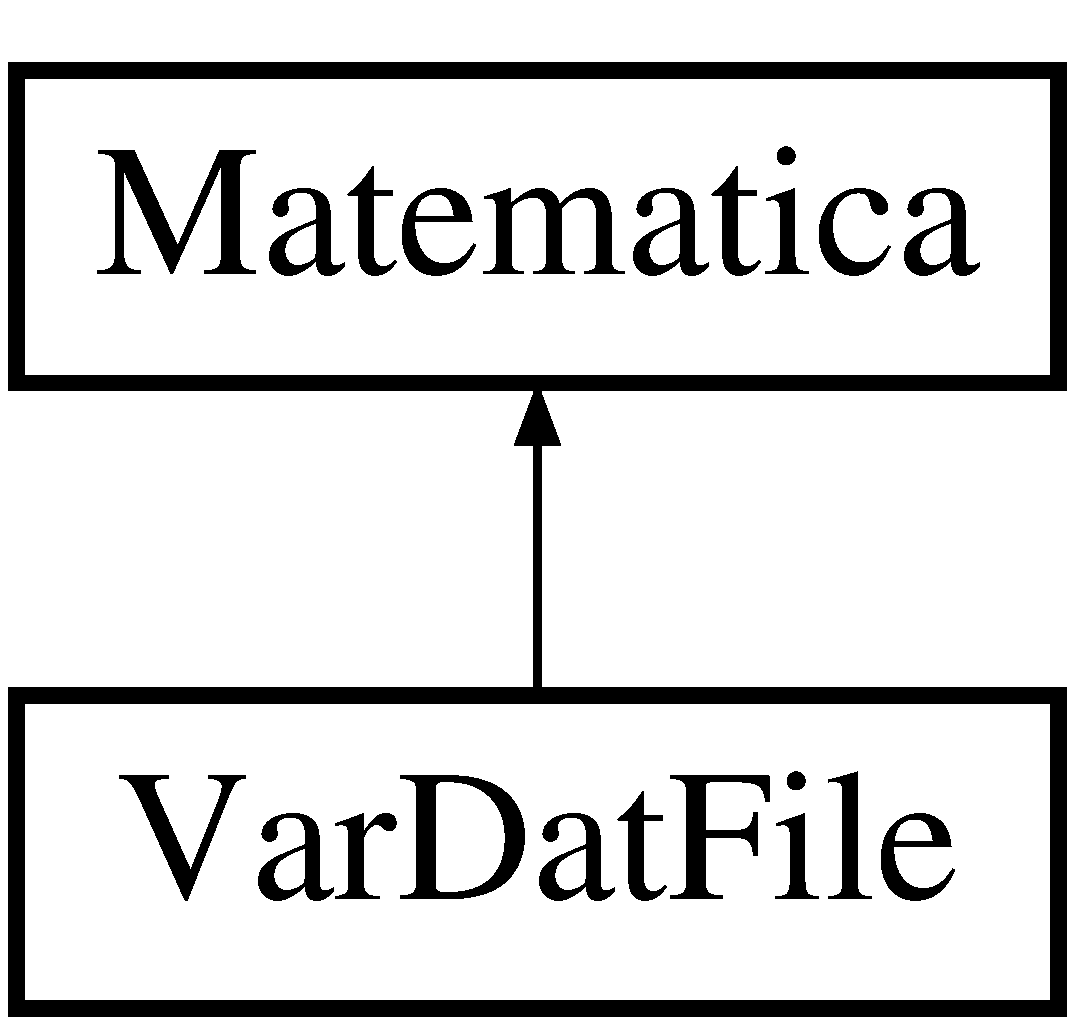
\includegraphics[height=2.000000cm]{classVarDatFile}
\end{center}
\end{figure}
\subsubsection*{\-Public \-Member \-Functions}
\begin{DoxyCompactItemize}
\item 
\hyperlink{classVarDatFile_a21fde0fe885a9c32bed3f479030b932f}{\-Var\-Dat\-File} (char $\ast$file, int \hyperlink{classVarDatFile_a6a683d7b3c08aafd7a5329b0d293eab6}{\-N\-Bin})
\begin{DoxyCompactList}\small\item\em \-Moltiplication factor for a scaled set (\-Media\-Mob) \end{DoxyCompactList}\item 
\hypertarget{classVarDatFile_aee213a28901788f8039811a1849fd829}{\hyperlink{classVarDatFile_aee213a28901788f8039811a1849fd829}{\-Var\-Dat\-File} (int \-Ext\-N\-Max, int \-Ext\-N\-Var, int \-Ext\-N\-Bin)}\label{classVarDatFile_aee213a28901788f8039811a1849fd829}

\begin{DoxyCompactList}\small\item\em \-Allocate the vector with a given size. \end{DoxyCompactList}\item 
\hypertarget{classVarDatFile_a8a83d164588d4aadbf15e250d29b5a6b}{\hyperlink{classVarDatFile_a8a83d164588d4aadbf15e250d29b5a6b}{\-Var\-Dat\-File} (double $\ast$$\ast$\-Ext\-St, int \-Ext\-N\-Max, int \-Ext\-N\-Var, int \-Ext\-N\-Bin)}\label{classVarDatFile_a8a83d164588d4aadbf15e250d29b5a6b}

\begin{DoxyCompactList}\small\item\em \-Point to the already allocated vector. \end{DoxyCompactList}\item 
\hypertarget{classVarDatFile_ac31e8053d3ade20d6b08259849c87976}{\hyperlink{classVarDatFile_ac31e8053d3ade20d6b08259849c87976}{\-Var\-Dat\-File} (char $\ast$$\ast$\-File\-List, int $\ast$\-Pos, int \-N\-File, int \-Values)}\label{classVarDatFile_ac31e8053d3ade20d6b08259849c87976}

\begin{DoxyCompactList}\small\item\em \-Load list. \end{DoxyCompactList}\item 
\hypertarget{classVarDatFile_acbe3dc1b93a2c0aa2cf310056bef0287}{\hyperlink{classVarDatFile_acbe3dc1b93a2c0aa2cf310056bef0287}{$\sim$\-Var\-Dat\-File} ()}\label{classVarDatFile_acbe3dc1b93a2c0aa2cf310056bef0287}

\begin{DoxyCompactList}\small\item\em \-Freeing. \end{DoxyCompactList}\item 
\hypertarget{classVarDatFile_acd5ad8eb7d2e19f9341bbd969b8781f4}{int \hyperlink{classVarDatFile_acd5ad8eb7d2e19f9341bbd969b8781f4}{\-Aggiungi} (char $\ast$file)}\label{classVarDatFile_acd5ad8eb7d2e19f9341bbd969b8781f4}

\begin{DoxyCompactList}\small\item\em \-Add the content of the file into the memory. \end{DoxyCompactList}\item 
\hypertarget{classVarDatFile_a63cfc9d080698099e7831515b4fa7625}{int \hyperlink{classVarDatFile_a63cfc9d080698099e7831515b4fa7625}{\-File\-Info} (\-F\-I\-L\-E $\ast$\-In\-F\-Ile, int $\ast$\-N\-Col)}\label{classVarDatFile_a63cfc9d080698099e7831515b4fa7625}

\begin{DoxyCompactList}\small\item\em \-Reads information contained in the file. \end{DoxyCompactList}\item 
\hypertarget{classVarDatFile_ade68053131c1d1ddd635f526f93e4ff3}{int \hyperlink{classVarDatFile_ade68053131c1d1ddd635f526f93e4ff3}{\-Read\-Line} (char $\ast$c\-Line, double $\ast$\-Value)}\label{classVarDatFile_ade68053131c1d1ddd635f526f93e4ff3}

\begin{DoxyCompactList}\small\item\em \-Reads a single line. \end{DoxyCompactList}\item 
\hypertarget{classVarDatFile_acfb2b7579c38d629e6585e6f60373783}{int \hyperlink{classVarDatFile_acfb2b7579c38d629e6585e6f60373783}{\-Read\-Line} (\-F\-I\-L\-E $\ast$\-In\-File, const char $\ast$\-Format,...)}\label{classVarDatFile_acfb2b7579c38d629e6585e6f60373783}

\begin{DoxyCompactList}\small\item\em \-Is it working? \end{DoxyCompactList}\item 
\hypertarget{classVarDatFile_ab6e65ce9879959397314adb9c1f3d5e6}{int \hyperlink{classVarDatFile_ab6e65ce9879959397314adb9c1f3d5e6}{\-Elab\-Segnale} (int \-N\-El\-Min, int \-N\-El\-Max)}\label{classVarDatFile_ab6e65ce9879959397314adb9c1f3d5e6}

\begin{DoxyCompactList}\small\item\em \-Do a generic elaboration. \end{DoxyCompactList}\item 
\hypertarget{classVarDatFile_a176c9a10a842e30206fe1ebece6917dc}{\hyperlink{structMOMENTI}{\-M\-O\-M\-E\-N\-T\-I} \hyperlink{classVarDatFile_a176c9a10a842e30206fe1ebece6917dc}{\-Distr\-Segnale} (int \-N\-El\-Min, int \-N\-El\-Max, int \-If\-Norm)}\label{classVarDatFile_a176c9a10a842e30206fe1ebece6917dc}

\begin{DoxyCompactList}\small\item\em \-Distribution of a signal. \end{DoxyCompactList}\item 
\hypertarget{classVarDatFile_a82c1693acb4e233005f36e72e10d8f84}{\hyperlink{structMOMENTI}{\-M\-O\-M\-E\-N\-T\-I} \hyperlink{classVarDatFile_a82c1693acb4e233005f36e72e10d8f84}{\-Distr\-Log\-Segnale} (int \-N\-El\-Min, int \-N\-El\-Max, int \-If\-Norm)}\label{classVarDatFile_a82c1693acb4e233005f36e72e10d8f84}

\begin{DoxyCompactList}\small\item\em \-Logarithmic distribution of a signal. \end{DoxyCompactList}\item 
\hypertarget{classVarDatFile_a368bdb3c4de9a07c0ce1ea7edb331778}{\hyperlink{structMOMENTI}{\-M\-O\-M\-E\-N\-T\-I} \hyperlink{classVarDatFile_a368bdb3c4de9a07c0ce1ea7edb331778}{\-Distr\-Exp\-Segnale} (int \-N\-El\-Min, int \-N\-El\-Max, int \-If\-Norm)}\label{classVarDatFile_a368bdb3c4de9a07c0ce1ea7edb331778}

\begin{DoxyCompactList}\small\item\em \-Exponential distribution of a signal. \end{DoxyCompactList}\item 
\hypertarget{classVarDatFile_a86ca74545b082ee1b6fc140c2d56b943}{\hyperlink{structMOMENTI}{\-M\-O\-M\-E\-N\-T\-I} \hyperlink{classVarDatFile_a86ca74545b082ee1b6fc140c2d56b943}{\-Distr\-Segnale} (int \-N\-El\-Min, int \-N\-El\-Max, double $\ast$\-Border, int \-If\-Norm)}\label{classVarDatFile_a86ca74545b082ee1b6fc140c2d56b943}

\begin{DoxyCompactList}\small\item\em \-Distribution of a signal. \end{DoxyCompactList}\item 
\hypertarget{classVarDatFile_a418f05ea3f8e69dbc49adeccddbb8d66}{\hyperlink{structMOMENTI}{\-M\-O\-M\-E\-N\-T\-I} \hyperlink{classVarDatFile_a418f05ea3f8e69dbc49adeccddbb8d66}{\-Distr\-Sign\-Err} (int \-N\-El\-Min, int \-N\-El\-Max, double $\ast$\-Border, int \-If\-Norm)}\label{classVarDatFile_a418f05ea3f8e69dbc49adeccddbb8d66}

\begin{DoxyCompactList}\small\item\em \-Distribution of a signal with error. \end{DoxyCompactList}\item 
\hypertarget{classVarDatFile_ac5e7b70f512f6a7a4dd83e942a65537a}{\hyperlink{structMOMENTI}{\-M\-O\-M\-E\-N\-T\-I} \hyperlink{classVarDatFile_ac5e7b70f512f6a7a4dd83e942a65537a}{\-Distr\-Gauss\-Segnale} (int \-El\-Min, int \-El\-Max, int \-If\-Norm)}\label{classVarDatFile_ac5e7b70f512f6a7a4dd83e942a65537a}

\begin{DoxyCompactList}\small\item\em \-Tests a gaussian distribution of the signal. \end{DoxyCompactList}\item 
\hypertarget{classVarDatFile_acc46e4201d7bdf288601a253bd569ed0}{\hyperlink{structMOMENTI}{\-M\-O\-M\-E\-N\-T\-I} \hyperlink{classVarDatFile_acc46e4201d7bdf288601a253bd569ed0}{\-Weight\-Average\-Set} (int \-Coord\-Y, int \-El\-Min, int \-El\-Max)}\label{classVarDatFile_acc46e4201d7bdf288601a253bd569ed0}

\begin{DoxyCompactList}\small\item\em \-Weighted distribution. \end{DoxyCompactList}\item 
\hypertarget{classVarDatFile_ab0b5ef5ddc23685148eda453b09ba2f5}{void \hyperlink{classVarDatFile_ab0b5ef5ddc23685148eda453b09ba2f5}{\-Distr\-Sign\-Sample} (int \-El\-Min, int \-El\-Max, double $\ast$$\ast$\-Distr, int \-N\-Sample, int \-If\-Norm, double $\ast$x\-Bound)}\label{classVarDatFile_ab0b5ef5ddc23685148eda453b09ba2f5}

\begin{DoxyCompactList}\small\item\em \-Distributions of data organized in different samples. \end{DoxyCompactList}\item 
\hypertarget{classVarDatFile_a1454407975f3283a2786d1f5a30c537f}{int \hyperlink{classVarDatFile_a1454407975f3283a2786d1f5a30c537f}{\-Spettro\-Segnale} (int \-N\-El\-Min, int \-N\-El\-Max)}\label{classVarDatFile_a1454407975f3283a2786d1f5a30c537f}

\begin{DoxyCompactList}\small\item\em \-Calculate the spectrum. \end{DoxyCompactList}\item 
\hypertarget{classVarDatFile_a3a27fb16efc015da73aeb6d511d87252}{void \hyperlink{classVarDatFile_a3a27fb16efc015da73aeb6d511d87252}{\-Spe\-Line} (int \-El\-Min, int \-El\-Max, int \hyperlink{classVarDatFile_a6a683d7b3c08aafd7a5329b0d293eab6}{\-N\-Bin}, double $\ast$\-Spe)}\label{classVarDatFile_a3a27fb16efc015da73aeb6d511d87252}

\begin{DoxyCompactList}\small\item\em \-Spectrum of a sequence of lines. \end{DoxyCompactList}\item 
\hypertarget{classVarDatFile_a0e495e387b74aaa6d55510a945236064}{int \hyperlink{classVarDatFile_a0e495e387b74aaa6d55510a945236064}{\-Normalizza\-Segnale} (int \-N\-El\-Min, int \-N\-El\-Max)}\label{classVarDatFile_a0e495e387b74aaa6d55510a945236064}

\begin{DoxyCompactList}\small\item\em \-Normalize the signal. \end{DoxyCompactList}\item 
\hypertarget{classVarDatFile_a2f01ea77260e98cb7edbb892988fd687}{int \hyperlink{classVarDatFile_a2f01ea77260e98cb7edbb892988fd687}{\-Normalizza\-Inter} ()}\label{classVarDatFile_a2f01ea77260e98cb7edbb892988fd687}

\begin{DoxyCompactList}\small\item\em \-Normalize the intervals. \end{DoxyCompactList}\item 
\hypertarget{classVarDatFile_ab68c66ee2972197a35b5225793337637}{bool \hyperlink{classVarDatFile_ab68c66ee2972197a35b5225793337637}{\-Radice\-Segnale} ()}\label{classVarDatFile_ab68c66ee2972197a35b5225793337637}

\begin{DoxyCompactList}\small\item\em \-Transforms the signal into its square root. \end{DoxyCompactList}\item 
\hypertarget{classVarDatFile_a9aaf71e7c7f27423252d8359f746e4ff}{int \hyperlink{classVarDatFile_a9aaf71e7c7f27423252d8359f746e4ff}{\-Autocor\-Segnale} (int \-N\-El\-Min, int \-N\-El\-Max)}\label{classVarDatFile_a9aaf71e7c7f27423252d8359f746e4ff}

\begin{DoxyCompactList}\small\item\em \-Autocorrelation of the signal. \end{DoxyCompactList}\item 
\hypertarget{classVarDatFile_a6489d2b859470a4e034bc4f795336ae8}{double \hyperlink{classVarDatFile_a6489d2b859470a4e034bc4f795336ae8}{\-Sum\-Segnale} (int \-Coord\-Y, int \-N\-El\-Min, int \-N\-El\-Max)}\label{classVarDatFile_a6489d2b859470a4e034bc4f795336ae8}

\begin{DoxyCompactList}\small\item\em \-Sum the values between \-El\-Min and \-El\-Max. \end{DoxyCompactList}\item 
\hypertarget{classVarDatFile_a43b771dc3214a9a36b2aa2a91ffb8edb}{double \hyperlink{classVarDatFile_a43b771dc3214a9a36b2aa2a91ffb8edb}{\-Int\-Segnale} ()}\label{classVarDatFile_a43b771dc3214a9a36b2aa2a91ffb8edb}

\begin{DoxyCompactList}\small\item\em \-Numerical integration of the signal. \end{DoxyCompactList}\item 
\hypertarget{classVarDatFile_a7a3685f3878bcb9e05a16bdadface9f9}{void \hyperlink{classVarDatFile_a7a3685f3878bcb9e05a16bdadface9f9}{\-Somma\-Segnali} ()}\label{classVarDatFile_a7a3685f3878bcb9e05a16bdadface9f9}

\begin{DoxyCompactList}\small\item\em \-Sums all the y\-Coordinates. \end{DoxyCompactList}\item 
\hypertarget{classVarDatFile_a982e54013ecdf9dcadead5247def28be}{void \hyperlink{classVarDatFile_a982e54013ecdf9dcadead5247def28be}{\-Average\-Ordinate} (int \-El\-Min, int \-El\-Max, double $\ast$\-Distr, double $\ast$x\-Bound)}\label{classVarDatFile_a982e54013ecdf9dcadead5247def28be}

\begin{DoxyCompactList}\small\item\em \-Average of all ordinate. \end{DoxyCompactList}\item 
\hypertarget{classVarDatFile_a9bb9fb6bb48e6c597ba31a271e1be613}{void \hyperlink{classVarDatFile_a9bb9fb6bb48e6c597ba31a271e1be613}{\-Punta} (int n)}\label{classVarDatFile_a9bb9fb6bb48e6c597ba31a271e1be613}

\begin{DoxyCompactList}\small\item\em \-Points to a different column. \end{DoxyCompactList}\item 
\hypertarget{classVarDatFile_ad2642e22b919be30857ed370e8d22acc}{void \hyperlink{classVarDatFile_ad2642e22b919be30857ed370e8d22acc}{\-Punta} (double $\ast$$\ast$\-Ext\-St, int n)}\label{classVarDatFile_ad2642e22b919be30857ed370e8d22acc}

\begin{DoxyCompactList}\small\item\em \-Points to an external pointer, probably not working. \end{DoxyCompactList}\item 
\hypertarget{classVarDatFile_a3459dd82527a16fe552b58f9bbb3beca}{void \hyperlink{classVarDatFile_a3459dd82527a16fe552b58f9bbb3beca}{\-Punta} (double $\ast$\hyperlink{classVarDatFile_a0e376f4d59c4a98b04daf57047cad5f9}{sp}, int n)}\label{classVarDatFile_a3459dd82527a16fe552b58f9bbb3beca}

\begin{DoxyCompactList}\small\item\em \-Point an external pointer to the private memory. \end{DoxyCompactList}\item 
\hypertarget{classVarDatFile_ad4ea52d09ccc5d7b38b2952c4fdaa1a6}{void \hyperlink{classVarDatFile_ad4ea52d09ccc5d7b38b2952c4fdaa1a6}{\-Punta\-Int} (double $\ast$\hyperlink{classVarDatFile_a0e376f4d59c4a98b04daf57047cad5f9}{sp})}\label{classVarDatFile_ad4ea52d09ccc5d7b38b2952c4fdaa1a6}

\begin{DoxyCompactList}\small\item\em \-Point the internal pointer to an external memory. \end{DoxyCompactList}\item 
\hypertarget{classVarDatFile_a5a90e3f39948e4e3e870c9d83af5eef0}{void \hyperlink{classVarDatFile_a5a90e3f39948e4e3e870c9d83af5eef0}{\-Derivata\-Segnale} ()}\label{classVarDatFile_a5a90e3f39948e4e3e870c9d83af5eef0}

\begin{DoxyCompactList}\small\item\em \-Points the function \-Elab to the derivative, probably not working. \end{DoxyCompactList}\item 
\hypertarget{classVarDatFile_af79a8603c9c35b3f0b3018090697fca8}{void \hyperlink{classVarDatFile_af79a8603c9c35b3f0b3018090697fca8}{\-Varie\-Segnale} ()}\label{classVarDatFile_af79a8603c9c35b3f0b3018090697fca8}

\begin{DoxyCompactList}\small\item\em \-Points the function \-Elab to the square gradient, probably not working. \end{DoxyCompactList}\item 
\hypertarget{classVarDatFile_a72776345635c4c0717fce1b11f03d625}{void \hyperlink{classVarDatFile_a72776345635c4c0717fce1b11f03d625}{\-Modulo\-Segnale} ()}\label{classVarDatFile_a72776345635c4c0717fce1b11f03d625}

\begin{DoxyCompactList}\small\item\em \-Points the function \-Elab to the module, probably not working. \end{DoxyCompactList}\item 
\hypertarget{classVarDatFile_aa8c3dec822e735ee8835f0e19d8b15a3}{double \hyperlink{classVarDatFile_aa8c3dec822e735ee8835f0e19d8b15a3}{\-Varie\-Segnale} (int \-N\-El\-Min, int \-N\-El\-Max)}\label{classVarDatFile_aa8c3dec822e735ee8835f0e19d8b15a3}

\begin{DoxyCompactList}\small\item\em \-A generic function to be edit. \end{DoxyCompactList}\item 
\hypertarget{classVarDatFile_ad705e28f47a98707e3dd3c83d86e85b3}{\hyperlink{structRETTA}{\-R\-E\-T\-T\-A} \hyperlink{classVarDatFile_ad705e28f47a98707e3dd3c83d86e85b3}{\-Inter\-Rett\-Segnale} (int \-Coord\-Y, int \-N\-El\-Min, int \-N\-El\-Max, int \-Log\-Log)}\label{classVarDatFile_ad705e28f47a98707e3dd3c83d86e85b3}

\begin{DoxyCompactList}\small\item\em \-Computes a liner fit. \end{DoxyCompactList}\item 
\hypertarget{classVarDatFile_a7e8033bdeb05d587eb6ce7dedf3ffe8b}{\hyperlink{structRETTA}{\-R\-E\-T\-T\-A} \hyperlink{classVarDatFile_a7e8033bdeb05d587eb6ce7dedf3ffe8b}{\-Inter\-Exp\-Segnale} (int \-Coord\-Y, int \-N\-El\-Min, int \-N\-El\-Max, int \-Log\-Log)}\label{classVarDatFile_a7e8033bdeb05d587eb6ce7dedf3ffe8b}

\begin{DoxyCompactList}\small\item\em \-Computes a exponential fit. \end{DoxyCompactList}\item 
\hypertarget{classVarDatFile_a77d32f56ea66cb8070e708766c7577ea}{\hyperlink{structMOMENTI}{\-M\-O\-M\-E\-N\-T\-I} \hyperlink{classVarDatFile_a77d32f56ea66cb8070e708766c7577ea}{\-Inter\-Gauss\-Segnale} (int \-Coord\-Y, int \-N\-El\-Min, int \-N\-El\-Max, int \-Log\-Log)}\label{classVarDatFile_a77d32f56ea66cb8070e708766c7577ea}

\begin{DoxyCompactList}\small\item\em \-Computes a \-Gaussian fit. \end{DoxyCompactList}\item 
\hypertarget{classVarDatFile_a670b0120b56b71deeb92a07dbc2d1a93}{\hyperlink{structPARABOLA}{\-P\-A\-R\-A\-B\-O\-L\-A} \hyperlink{classVarDatFile_a670b0120b56b71deeb92a07dbc2d1a93}{\-Parabola\-Segnale} (int \-Coord\-Y, int \-N\-El\-Min, int \-N\-El\-Max, int \-Log\-Log)}\label{classVarDatFile_a670b0120b56b71deeb92a07dbc2d1a93}

\begin{DoxyCompactList}\small\item\em \-Computes a parabolic fit. \end{DoxyCompactList}\item 
\hypertarget{classVarDatFile_af61093b90aceaaeaabfaf6364db43abf}{int \hyperlink{classVarDatFile_af61093b90aceaaeaabfaf6364db43abf}{\-Media\-Mob\-Segnale} (int)}\label{classVarDatFile_af61093b90aceaaeaabfaf6364db43abf}

\begin{DoxyCompactList}\small\item\em \-Running average. \end{DoxyCompactList}\item 
int \hyperlink{classVarDatFile_ad6521d627ba809d5e253cefcd5090491}{\-Weight\-Histo\-Sign} (int \-N\-Histo)
\begin{DoxyCompactList}\small\item\em \-Weighted histogram analysis. \end{DoxyCompactList}\item 
\hypertarget{classVarDatFile_aa6212bdcf240e866f234a41d6b98a224}{int \hyperlink{classVarDatFile_aa6212bdcf240e866f234a41d6b98a224}{\-Correla\-A\-Due\-Punti} (int dist)}\label{classVarDatFile_aa6212bdcf240e866f234a41d6b98a224}

\begin{DoxyCompactList}\small\item\em \-To point correlation at a distance dist. \end{DoxyCompactList}\item 
\hypertarget{classVarDatFile_ae1058d878c5370add56411e3998b9d51}{void \hyperlink{classVarDatFile_ae1058d878c5370add56411e3998b9d51}{\-Autosimilarita\-Segnale} (int)}\label{classVarDatFile_ae1058d878c5370add56411e3998b9d51}

\begin{DoxyCompactList}\small\item\em \-Selfsimilarity. \end{DoxyCompactList}\item 
\hypertarget{classVarDatFile_af0b16f63863e97d7c86f9ac00e67f11b}{void \hyperlink{classVarDatFile_af0b16f63863e97d7c86f9ac00e67f11b}{\-Cambia\-N\-Bin} (int)}\label{classVarDatFile_af0b16f63863e97d7c86f9ac00e67f11b}

\begin{DoxyCompactList}\small\item\em \-Reallocate the pointer d\-Inter d\-Inter1. \end{DoxyCompactList}\item 
\hypertarget{classVarDatFile_ad399f5baf6ac6cda47416f07b69b3ca8}{void \hyperlink{classVarDatFile_ad399f5baf6ac6cda47416f07b69b3ca8}{\-Cambia\-Punti} ()}\label{classVarDatFile_ad399f5baf6ac6cda47416f07b69b3ca8}

\begin{DoxyCompactList}\small\item\em \-Copies \-Punti in \-Punti1 to store the information of the already elaborated array, to be fixed. \end{DoxyCompactList}\item 
\hypertarget{classVarDatFile_a9dcac18006ce057b8d78c847174c1362}{void \hyperlink{classVarDatFile_a9dcac18006ce057b8d78c847174c1362}{\-Print} ()}\label{classVarDatFile_a9dcac18006ce057b8d78c847174c1362}

\begin{DoxyCompactList}\small\item\em \-Prints the content in memory. \end{DoxyCompactList}\item 
\hypertarget{classVarDatFile_ae424c3360277f457eba79fd25b4eed3b}{void \hyperlink{classVarDatFile_ae424c3360277f457eba79fd25b4eed3b}{\-Sort} ()}\label{classVarDatFile_ae424c3360277f457eba79fd25b4eed3b}

\begin{DoxyCompactList}\small\item\em \-Sort with respect to a coordinate. \end{DoxyCompactList}\item 
\hypertarget{classVarDatFile_a15ad052575da97bec5b2bad38a52385e}{void \hyperlink{classVarDatFile_a15ad052575da97bec5b2bad38a52385e}{\-Scrivi\-Punti} (char $\ast$file)}\label{classVarDatFile_a15ad052575da97bec5b2bad38a52385e}

\begin{DoxyCompactList}\small\item\em \-Writes the content of the elaborated array. \end{DoxyCompactList}\item 
\hypertarget{classVarDatFile_acc513a8bb6bda4c6bbf7832a9dcdd19a}{void \hyperlink{classVarDatFile_acc513a8bb6bda4c6bbf7832a9dcdd19a}{\-Scrivi\-File} (char $\ast$file, int \-Coord\-Y, int \-Log\-Log, int \-N\-Vis\-Min, int \-N\-Vis\-Max)}\label{classVarDatFile_acc513a8bb6bda4c6bbf7832a9dcdd19a}

\begin{DoxyCompactList}\small\item\em \-Writes the content of the pointed vector. \end{DoxyCompactList}\item 
\hypertarget{classVarDatFile_aef5b55b7d54d1a01e9e507d3c4d23e4d}{void \hyperlink{classVarDatFile_aef5b55b7d54d1a01e9e507d3c4d23e4d}{\-Scrivi\-Tutto} (char $\ast$file, int \-Log\-Log, int \-N\-Vis\-Min, int \-N\-Vis\-Max)}\label{classVarDatFile_aef5b55b7d54d1a01e9e507d3c4d23e4d}

\begin{DoxyCompactList}\small\item\em \-Writes all the content in memory. \end{DoxyCompactList}\item 
\hypertarget{classVarDatFile_a50acf56d68429e9660e2bfc4f7530521}{void \hyperlink{classVarDatFile_a50acf56d68429e9660e2bfc4f7530521}{\-Rescale\-To\-Bulk} (char $\ast$\-F\-Name)}\label{classVarDatFile_a50acf56d68429e9660e2bfc4f7530521}

\begin{DoxyCompactList}\small\item\em \-Rescale to bulk. \end{DoxyCompactList}\item 
\hypertarget{classVarDatFile_a87e9980dd97eda060a3dcaddd1d692d4}{void \hyperlink{classVarDatFile_a87e9980dd97eda060a3dcaddd1d692d4}{\-Export\-Txvl} (char $\ast$\-F\-Name, int \-N\-El\-Min, int \-N\-El\-Max)}\label{classVarDatFile_a87e9980dd97eda060a3dcaddd1d692d4}

\begin{DoxyCompactList}\small\item\em \-Export in the txvl file format. \end{DoxyCompactList}\item 
\hypertarget{classVarDatFile_ace7cb52bc9334449375e6e0456161120}{void \hyperlink{classVarDatFile_ace7cb52bc9334449375e6e0456161120}{\-Tec\-Plot} (char $\ast$\-F\-Name)}\label{classVarDatFile_ace7cb52bc9334449375e6e0456161120}

\begin{DoxyCompactList}\small\item\em \-Export a contour plot. \end{DoxyCompactList}\item 
void \hyperlink{classVarDatFile_a38ef005b54f94a56824e7240876e9c03}{\-Punti\-Alloc} ()
\begin{DoxyCompactList}\small\item\em \-Allocates. \end{DoxyCompactList}\item 
\hypertarget{classVarDatFile_aab87873039820cc1aca0c444c43d9a5e}{void \hyperlink{classVarDatFile_aab87873039820cc1aca0c444c43d9a5e}{\-Punti\-Free} ()}\label{classVarDatFile_aab87873039820cc1aca0c444c43d9a5e}

\begin{DoxyCompactList}\small\item\em \-Free \-Punti if it is allocated. \end{DoxyCompactList}\item 
\hypertarget{classVarDatFile_aff25aa77a033788903eee04852e24cb6}{int \hyperlink{classVarDatFile_aff25aa77a033788903eee04852e24cb6}{p\-N\-Var} ()}\label{classVarDatFile_aff25aa77a033788903eee04852e24cb6}

\begin{DoxyCompactList}\small\item\em \-Print the number of variables. \end{DoxyCompactList}\item 
\hypertarget{classVarDatFile_a9dcafc8ed48e17a6980b121cb76e56fa}{int \hyperlink{classVarDatFile_a9dcafc8ed48e17a6980b121cb76e56fa}{p\-N\-Max} ()}\label{classVarDatFile_a9dcafc8ed48e17a6980b121cb76e56fa}

\begin{DoxyCompactList}\small\item\em \-Print the maximum number of data in the array. \end{DoxyCompactList}\item 
\hypertarget{classVarDatFile_a48d99b519007370b7b0657a1f6665c27}{int \hyperlink{classVarDatFile_a48d99b519007370b7b0657a1f6665c27}{p\-N\-Row} (int \-Coord\-Y)}\label{classVarDatFile_a48d99b519007370b7b0657a1f6665c27}

\begin{DoxyCompactList}\small\item\em \-Print the maximum number of data for the column. \end{DoxyCompactList}\item 
\hypertarget{classVarDatFile_a8209ef54a8a7b2173ce491cba2008c56}{void \hyperlink{classVarDatFile_a8209ef54a8a7b2173ce491cba2008c56}{p\-Glob\-Border} (double $\ast$x\-Min, double $\ast$x\-Max, double $\ast$y\-Min, double $\ast$y\-Max)}\label{classVarDatFile_a8209ef54a8a7b2173ce491cba2008c56}

\begin{DoxyCompactList}\small\item\em \-Print global borders. \end{DoxyCompactList}\item 
double \hyperlink{classVarDatFile_a2b1e58fd6ed28920042681b8e27f369f}{\-Val} (int \-Coord\-Y, int n)
\begin{DoxyCompactList}\small\item\em \-Value at the position. \end{DoxyCompactList}\item 
double \hyperlink{classVarDatFile_a3f23e3592344b829371e42e77ed02d15}{\-Abscissa} (int \-Coord\-Y, int n)
\begin{DoxyCompactList}\small\item\em \-Value of the \-Abscissa at position. \end{DoxyCompactList}\item 
double \hyperlink{classVarDatFile_aceb09b397fee83699a8b810fcaa02d26}{p\-Punti} (int n)
\begin{DoxyCompactList}\small\item\em \-Value of the elaborated array at position. \end{DoxyCompactList}\item 
double \hyperlink{classVarDatFile_a3a14794e0583788d1cd614bfa4aa4a17}{p\-Punti\-Err} (int n)
\begin{DoxyCompactList}\small\item\em \-Value of the error array at postion. \end{DoxyCompactList}\item 
\hypertarget{classVarDatFile_a46c8b0d765845804061b9ed216e96555}{void \hyperlink{classVarDatFile_a46c8b0d765845804061b9ed216e96555}{p\-Min\-Max\-Glob} (int \-N\-Vis\-Min, int \-N\-Vis\-Max)}\label{classVarDatFile_a46c8b0d765845804061b9ed216e96555}

\begin{DoxyCompactList}\small\item\em \-Find the borders globally. \end{DoxyCompactList}\item 
\hypertarget{classVarDatFile_a3842ee06d27e5ffab8330b9a42abe651}{double \hyperlink{classVarDatFile_a3842ee06d27e5ffab8330b9a42abe651}{p\-Max\-Glob} (int \-N\-Vis\-Min, int \-N\-Vis\-Max)}\label{classVarDatFile_a3842ee06d27e5ffab8330b9a42abe651}

\begin{DoxyCompactList}\small\item\em \-Print the maximum of all sets. \end{DoxyCompactList}\item 
\hypertarget{classVarDatFile_abb5cfc85ebb62f7226afe58ab7f70f68}{double \hyperlink{classVarDatFile_abb5cfc85ebb62f7226afe58ab7f70f68}{p\-Min\-Glob} (int \-N\-Vis\-Min, int \-N\-Vis\-Max)}\label{classVarDatFile_abb5cfc85ebb62f7226afe58ab7f70f68}

\begin{DoxyCompactList}\small\item\em \-Print the minimum of all sets. \end{DoxyCompactList}\item 
\hypertarget{classVarDatFile_a6c9b0181c2505369c375bcb91f36409f}{double \hyperlink{classVarDatFile_a6c9b0181c2505369c375bcb91f36409f}{px\-Min\-Glob} (int \-N\-Vis\-Min, int \-N\-Vis\-Max)}\label{classVarDatFile_a6c9b0181c2505369c375bcb91f36409f}

\begin{DoxyCompactList}\small\item\em \-Print the abscissa minimum of all sets. \end{DoxyCompactList}\item 
\hypertarget{classVarDatFile_ab594ce06a5fb24acf5c812f2d02fde06}{double \hyperlink{classVarDatFile_ab594ce06a5fb24acf5c812f2d02fde06}{px\-Max\-Glob} (int \-N\-Vis\-Min, int \-N\-Vis\-Max)}\label{classVarDatFile_ab594ce06a5fb24acf5c812f2d02fde06}

\begin{DoxyCompactList}\small\item\em \-Print the abscissa maximum of all sets. \end{DoxyCompactList}\item 
double \hyperlink{classVarDatFile_a3aea9835fc67f13c5b334e1a34af1be9}{p\-Max} (int \-Coord\-Y, int \-N\-Vis\-Min, int \-N\-Vis\-Max)
\begin{DoxyCompactList}\small\item\em \-Print the maximum of the column. \end{DoxyCompactList}\item 
double \hyperlink{classVarDatFile_afd9d7e4b40e8991b685d17cb65a38441}{p\-Min} (int \-Coord\-Y, int \-N\-Vis\-Min, int \-N\-Vis\-Max)
\begin{DoxyCompactList}\small\item\em \-Print the minimum of the column. \end{DoxyCompactList}\item 
\hypertarget{classVarDatFile_ad89c34d0afecf90978d5e36bf57e1bf0}{double \hyperlink{classVarDatFile_ad89c34d0afecf90978d5e36bf57e1bf0}{p\-Max\-Glob\-Log} (int \-N\-Vis\-Min, int \-N\-Vis\-Max)}\label{classVarDatFile_ad89c34d0afecf90978d5e36bf57e1bf0}

\begin{DoxyCompactList}\small\item\em \-Print the maximum of all sets. \end{DoxyCompactList}\item 
\hypertarget{classVarDatFile_ad47c958de7bca595ab42666050cac660}{double \hyperlink{classVarDatFile_ad47c958de7bca595ab42666050cac660}{p\-Min\-Glob\-Log} (int \-N\-Vis\-Min, int \-N\-Vis\-Max)}\label{classVarDatFile_ad47c958de7bca595ab42666050cac660}

\begin{DoxyCompactList}\small\item\em \-Print the minimum of all sets. \end{DoxyCompactList}\item 
double \hyperlink{classVarDatFile_abb42c2238af97f451a3ebf3226d13639}{p\-Max\-Log} (int \-Coord\-Y, int \-N\-Vis\-Min, int \-N\-Vis\-Max)
\begin{DoxyCompactList}\small\item\em \-Print the maximum of the column. \end{DoxyCompactList}\item 
double \hyperlink{classVarDatFile_af5ebcfc4c951d36ead08fdc20974b5ff}{p\-Min\-Log} (int \-Coord\-Y, int \-N\-Vis\-Min, int \-N\-Vis\-Max)
\begin{DoxyCompactList}\small\item\em \-Print the minimum of the column. \end{DoxyCompactList}\item 
double \hyperlink{classVarDatFile_ac9b6015f7712a2bffde3a609145331af}{p\-Inter} (int n)
\begin{DoxyCompactList}\small\item\em \-Print the postion. \end{DoxyCompactList}\item 
double \hyperlink{classVarDatFile_ab59237e1fbf8ee4c45f7f189799ed008}{p\-Error} (int n)
\begin{DoxyCompactList}\small\item\em \-Print the postion. \end{DoxyCompactList}\item 
double \hyperlink{classVarDatFile_a31c516fdbe042c50ffdf5d3dc74521ab}{p\-Inter1} (int n)
\begin{DoxyCompactList}\small\item\em \-Print the postion. \end{DoxyCompactList}\item 
double \hyperlink{classVarDatFile_a9998056e2576481a913421ae6e148179}{\-Punti\-Min} ()
\begin{DoxyCompactList}\small\item\em \-Print the minimum of. \end{DoxyCompactList}\item 
double \hyperlink{classVarDatFile_a0a3ba11d08ae946dfdf46d0b33047211}{\-Punti\-Max} ()
\begin{DoxyCompactList}\small\item\em \-Print the maximum of. \end{DoxyCompactList}\item 
\hypertarget{classVarDatFile_a2d7aa499f16ec4d2e15ac60bccbb8441}{int \hyperlink{classVarDatFile_a2d7aa499f16ec4d2e15ac60bccbb8441}{\-Is\-Abscissa} (int \-Col)}\label{classVarDatFile_a2d7aa499f16ec4d2e15ac60bccbb8441}

\begin{DoxyCompactList}\small\item\em \-If the column is an ascissa. \end{DoxyCompactList}\item 
\hypertarget{classVarDatFile_a79be07c83bc49d7f5e55c64944ed6304}{int \hyperlink{classVarDatFile_a79be07c83bc49d7f5e55c64944ed6304}{p\-Ref\-Absc} (int \-Col)}\label{classVarDatFile_a79be07c83bc49d7f5e55c64944ed6304}

\begin{DoxyCompactList}\small\item\em \-If the column is an ascissa. \end{DoxyCompactList}\item 
\hypertarget{classVarDatFile_a0b6ccc25f21f2a83096da6af6ea943e3}{int \hyperlink{classVarDatFile_a0b6ccc25f21f2a83096da6af6ea943e3}{p\-Set\-N\-Max} (int \-Col)}\label{classVarDatFile_a0b6ccc25f21f2a83096da6af6ea943e3}

\begin{DoxyCompactList}\small\item\em \-If the column is an ascissa. \end{DoxyCompactList}\item 
\hypertarget{classVarDatFile_a5c788a95c78a3da32eaac2f2f994de58}{int \hyperlink{classVarDatFile_a5c788a95c78a3da32eaac2f2f994de58}{\-Is\-Sequence} (int \-Col)}\label{classVarDatFile_a5c788a95c78a3da32eaac2f2f994de58}

\begin{DoxyCompactList}\small\item\em \-If the column is an ascissa. \end{DoxyCompactList}\item 
\hypertarget{classVarDatFile_a00eaf560508e46c0949042ab38af99de}{void \hyperlink{classVarDatFile_a00eaf560508e46c0949042ab38af99de}{\-Imp\-Sequence} (int \-Col)}\label{classVarDatFile_a00eaf560508e46c0949042ab38af99de}

\begin{DoxyCompactList}\small\item\em \-Set the natural sequence as abscissa for the column \-Col. \end{DoxyCompactList}\item 
\hypertarget{classVarDatFile_ad0ccdbdedaf66f5c01e3b850148a6b00}{void \hyperlink{classVarDatFile_ad0ccdbdedaf66f5c01e3b850148a6b00}{\-Imp\-Sequence} ()}\label{classVarDatFile_ad0ccdbdedaf66f5c01e3b850148a6b00}

\begin{DoxyCompactList}\small\item\em \-Set the natural sequence as abscissa for all sets. \end{DoxyCompactList}\item 
\hypertarget{classVarDatFile_a963c1d12c9e593a16748f229bc5bd11f}{void \hyperlink{classVarDatFile_a963c1d12c9e593a16748f229bc5bd11f}{\-Imp\-Coord\-X} (int v\-Abs)}\label{classVarDatFile_a963c1d12c9e593a16748f229bc5bd11f}

\begin{DoxyCompactList}\small\item\em \-Set the columns for the x array. \end{DoxyCompactList}\item 
\hypertarget{classVarDatFile_ac4e4ea335271e56d3a3dbc54bf0e8847}{void \hyperlink{classVarDatFile_ac4e4ea335271e56d3a3dbc54bf0e8847}{\-Imp\-Coord\-X} (int v\-Set, int v\-Abs)}\label{classVarDatFile_ac4e4ea335271e56d3a3dbc54bf0e8847}

\begin{DoxyCompactList}\small\item\em \-Set the column for the x array. \end{DoxyCompactList}\item 
\hypertarget{classVarDatFile_a4b08a81fa612f8cbeabb3618624fe7ca}{void \hyperlink{classVarDatFile_a4b08a81fa612f8cbeabb3618624fe7ca}{\-Imp\-Coord\-Y} (int \-Ext)}\label{classVarDatFile_a4b08a81fa612f8cbeabb3618624fe7ca}

\begin{DoxyCompactList}\small\item\em \-Set the column for the y array. \end{DoxyCompactList}\item 
\hypertarget{classVarDatFile_a589e6b70b557686f8a829acf53ec6b0c}{void \hyperlink{classVarDatFile_a589e6b70b557686f8a829acf53ec6b0c}{set\-X\-Formula} (char $\ast$str)}\label{classVarDatFile_a589e6b70b557686f8a829acf53ec6b0c}

\begin{DoxyCompactList}\small\item\em \-Set the value of \-X\-Formula. \end{DoxyCompactList}\item 
\hypertarget{classVarDatFile_adb4227dfb05be39d72d1b89cdc44eb5a}{void \hyperlink{classVarDatFile_adb4227dfb05be39d72d1b89cdc44eb5a}{set\-Y\-Formula} (char $\ast$str)}\label{classVarDatFile_adb4227dfb05be39d72d1b89cdc44eb5a}

\begin{DoxyCompactList}\small\item\em \-Set the value of \-Y\-Formula. \end{DoxyCompactList}\item 
\hypertarget{classVarDatFile_ae1b551cc51c9d556342b27b466a7c7cb}{void \hyperlink{classVarDatFile_ae1b551cc51c9d556342b27b466a7c7cb}{\-Reverse} ()}\label{classVarDatFile_ae1b551cc51c9d556342b27b466a7c7cb}

\begin{DoxyCompactList}\small\item\em \-Reverse the sets. \end{DoxyCompactList}\item 
\hypertarget{classVarDatFile_a42240e743f2a3ea3b430b915e50c5350}{int \hyperlink{classVarDatFile_a42240e743f2a3ea3b430b915e50c5350}{\-Smooth} (double \-Fact, int \-Coord\-Y, int \-N\-Vis\-Min, int \-N\-Vis\-Max)}\label{classVarDatFile_a42240e743f2a3ea3b430b915e50c5350}

\begin{DoxyCompactList}\small\item\em \-Smooth the line. \end{DoxyCompactList}\item 
\hypertarget{classVarDatFile_a12fe98e58e8262bcbf3aef114673673d}{void \hyperlink{classVarDatFile_a12fe98e58e8262bcbf3aef114673673d}{\-Smooth\-Gauss} (double \-Fact, int \-Coord\-Y, int \-N\-Vis\-Min, int \-N\-Vis\-Max)}\label{classVarDatFile_a12fe98e58e8262bcbf3aef114673673d}

\begin{DoxyCompactList}\small\item\em \-Smooth the line. \end{DoxyCompactList}\item 
\hypertarget{classVarDatFile_a6ab47ee0a227e3e13f042327b1f8fe33}{void \hyperlink{classVarDatFile_a6ab47ee0a227e3e13f042327b1f8fe33}{\-Double\-Dist\-Fluct} ()}\label{classVarDatFile_a6ab47ee0a227e3e13f042327b1f8fe33}

\begin{DoxyCompactList}\small\item\em \-Distribution of distances. \end{DoxyCompactList}\item 
\hypertarget{classVarDatFile_aedcb20a2169e38b38a21ad3f8bf011d2}{void \hyperlink{classVarDatFile_aedcb20a2169e38b38a21ad3f8bf011d2}{\-Write\-Formula} (char $\ast$\-Exit)}\label{classVarDatFile_aedcb20a2169e38b38a21ad3f8bf011d2}

\begin{DoxyCompactList}\small\item\em \-Execute a formula defined in \-X\-Formula and \-Y\-Formula. \end{DoxyCompactList}\item 
\hypertarget{classVarDatFile_ac6c6d90214b93afffeab31fd2bbe5715}{char $\ast$ \hyperlink{classVarDatFile_ac6c6d90214b93afffeab31fd2bbe5715}{\-Print\-Header} ()}\label{classVarDatFile_ac6c6d90214b93afffeab31fd2bbe5715}

\begin{DoxyCompactList}\small\item\em \-Print the header. \end{DoxyCompactList}\end{DoxyCompactItemize}
\subsubsection*{\-Public \-Attributes}
\begin{DoxyCompactItemize}
\item 
\hypertarget{classVarDatFile_a6a683d7b3c08aafd7a5329b0d293eab6}{int \hyperlink{classVarDatFile_a6a683d7b3c08aafd7a5329b0d293eab6}{\-N\-Bin}}\label{classVarDatFile_a6a683d7b3c08aafd7a5329b0d293eab6}

\begin{DoxyCompactList}\small\item\em \-Number of point of the distribution. \end{DoxyCompactList}\item 
\hypertarget{classVarDatFile_a0e376f4d59c4a98b04daf57047cad5f9}{double $\ast$ \hyperlink{classVarDatFile_a0e376f4d59c4a98b04daf57047cad5f9}{sp}}\label{classVarDatFile_a0e376f4d59c4a98b04daf57047cad5f9}

\begin{DoxyCompactList}\small\item\em \-Points to a column of st. \end{DoxyCompactList}\end{DoxyCompactItemize}


\subsubsection{\-Detailed \-Description}
\-Reads and stores a data file to be elaborated via \hyperlink{classMatematica}{\-Matematica}. 

\-Definition at line 26 of file \-Var\-Dat\-File.\-h.



\subsubsection{\-Constructor \& \-Destructor \-Documentation}
\hypertarget{classVarDatFile_a21fde0fe885a9c32bed3f479030b932f}{\index{\-Var\-Dat\-File@{\-Var\-Dat\-File}!\-Var\-Dat\-File@{\-Var\-Dat\-File}}
\index{\-Var\-Dat\-File@{\-Var\-Dat\-File}!VarDatFile@{\-Var\-Dat\-File}}
\paragraph[{\-Var\-Dat\-File}]{\setlength{\rightskip}{0pt plus 5cm}{\bf \-Var\-Dat\-File} (
\begin{DoxyParamCaption}
\item[{char $\ast$}]{file, }
\item[{int}]{\-N\-Bin}
\end{DoxyParamCaption}
)}}\label{classVarDatFile_a21fde0fe885a9c32bed3f479030b932f}


\-Moltiplication factor for a scaled set (\-Media\-Mob) 

\-Allocate the vectors reading from a file 

\subsubsection{\-Member \-Function \-Documentation}
\hypertarget{classVarDatFile_ad6521d627ba809d5e253cefcd5090491}{\index{\-Var\-Dat\-File@{\-Var\-Dat\-File}!\-Weight\-Histo\-Sign@{\-Weight\-Histo\-Sign}}
\index{\-Weight\-Histo\-Sign@{\-Weight\-Histo\-Sign}!VarDatFile@{\-Var\-Dat\-File}}
\paragraph[{\-Weight\-Histo\-Sign}]{\setlength{\rightskip}{0pt plus 5cm}int {\bf \-Weight\-Histo\-Sign} (
\begin{DoxyParamCaption}
\item[{int}]{\-N\-Histo}
\end{DoxyParamCaption}
)}}\label{classVarDatFile_ad6521d627ba809d5e253cefcd5090491}


\-Weighted histogram analysis. 

\-Find the borders globally 

\-Definition at line 578 of file \-Var\-Dat\-File.\-cpp.



\-References \-Is\-Abscissa(), \-N\-Bin, p\-Min\-Max\-Glob(), and \-Matematica\-::\-Weight\-Histo().

\hypertarget{classVarDatFile_a38ef005b54f94a56824e7240876e9c03}{\index{\-Var\-Dat\-File@{\-Var\-Dat\-File}!\-Punti\-Alloc@{\-Punti\-Alloc}}
\index{\-Punti\-Alloc@{\-Punti\-Alloc}!VarDatFile@{\-Var\-Dat\-File}}
\paragraph[{\-Punti\-Alloc}]{\setlength{\rightskip}{0pt plus 5cm}void {\bf \-Punti\-Alloc} (
\begin{DoxyParamCaption}
{}
\end{DoxyParamCaption}
)}}\label{classVarDatFile_a38ef005b54f94a56824e7240876e9c03}


\-Allocates. 

\begin{DoxySeeAlso}{\-See also}
\-Punti if necessary 
\end{DoxySeeAlso}


\-Definition at line 900 of file \-Var\-Dat\-File.\-cpp.



\-Referenced by \-Autocor\-Segnale(), \-Autosimilarita\-Segnale(), \-Correla\-A\-Due\-Punti(), \-Distr\-Exp\-Segnale(), \-Distr\-Log\-Segnale(), \-Double\-Dist\-Fluct(), \-Elab\-Segnale(), \-Int\-Segnale(), \-Media\-Mob\-Segnale(), \-Radice\-Segnale(), \-Smooth(), \-Smooth\-Gauss(), \-Somma\-Segnali(), \-Spettro\-Segnale(), and \-Varie\-Segnale().

\hypertarget{classVarDatFile_a2b1e58fd6ed28920042681b8e27f369f}{\index{\-Var\-Dat\-File@{\-Var\-Dat\-File}!\-Val@{\-Val}}
\index{\-Val@{\-Val}!VarDatFile@{\-Var\-Dat\-File}}
\paragraph[{\-Val}]{\setlength{\rightskip}{0pt plus 5cm}double {\bf \-Val} (
\begin{DoxyParamCaption}
\item[{int}]{\-Coord\-Y, }
\item[{int}]{n}
\end{DoxyParamCaption}
)}}\label{classVarDatFile_a2b1e58fd6ed28920042681b8e27f369f}


\-Value at the position. 


\begin{DoxyParams}{\-Parameters}
{\em n} & in the column \\
\hline
{\em v} & \\
\hline
\end{DoxyParams}


\-Definition at line 657 of file \-Var\-Dat\-File.\-cpp.



\-References \-N\-Bin.



\-Referenced by \-Export\-Txvl(), and \-Tec\-Plot().

\hypertarget{classVarDatFile_a3f23e3592344b829371e42e77ed02d15}{\index{\-Var\-Dat\-File@{\-Var\-Dat\-File}!\-Abscissa@{\-Abscissa}}
\index{\-Abscissa@{\-Abscissa}!VarDatFile@{\-Var\-Dat\-File}}
\paragraph[{\-Abscissa}]{\setlength{\rightskip}{0pt plus 5cm}double {\bf \-Abscissa} (
\begin{DoxyParamCaption}
\item[{int}]{\-Coord\-Y, }
\item[{int}]{n}
\end{DoxyParamCaption}
)}}\label{classVarDatFile_a3f23e3592344b829371e42e77ed02d15}


\-Value of the \-Abscissa at position. 


\begin{DoxyParams}{\-Parameters}
{\em n} & \\
\hline
\end{DoxyParams}


\-Definition at line 667 of file \-Var\-Dat\-File.\-cpp.



\-Referenced by \-Average\-Ordinate(), \-Export\-Txvl(), p\-Min\-Max\-Glob(), \-Print(), \-Rescale\-To\-Bulk(), and \-Tec\-Plot().

\hypertarget{classVarDatFile_aceb09b397fee83699a8b810fcaa02d26}{\index{\-Var\-Dat\-File@{\-Var\-Dat\-File}!p\-Punti@{p\-Punti}}
\index{p\-Punti@{p\-Punti}!VarDatFile@{\-Var\-Dat\-File}}
\paragraph[{p\-Punti}]{\setlength{\rightskip}{0pt plus 5cm}double {\bf p\-Punti} (
\begin{DoxyParamCaption}
\item[{int}]{n}
\end{DoxyParamCaption}
)}}\label{classVarDatFile_aceb09b397fee83699a8b810fcaa02d26}


\-Value of the elaborated array at position. 


\begin{DoxyParams}{\-Parameters}
{\em n} & \\
\hline
\end{DoxyParams}


\-Definition at line 673 of file \-Var\-Dat\-File.\-cpp.

\hypertarget{classVarDatFile_a3a14794e0583788d1cd614bfa4aa4a17}{\index{\-Var\-Dat\-File@{\-Var\-Dat\-File}!p\-Punti\-Err@{p\-Punti\-Err}}
\index{p\-Punti\-Err@{p\-Punti\-Err}!VarDatFile@{\-Var\-Dat\-File}}
\paragraph[{p\-Punti\-Err}]{\setlength{\rightskip}{0pt plus 5cm}double {\bf p\-Punti\-Err} (
\begin{DoxyParamCaption}
\item[{int}]{n}
\end{DoxyParamCaption}
)}}\label{classVarDatFile_a3a14794e0583788d1cd614bfa4aa4a17}


\-Value of the error array at postion. 


\begin{DoxyParams}{\-Parameters}
{\em n} & \\
\hline
\end{DoxyParams}


\-Definition at line 680 of file \-Var\-Dat\-File.\-cpp.

\hypertarget{classVarDatFile_a3aea9835fc67f13c5b334e1a34af1be9}{\index{\-Var\-Dat\-File@{\-Var\-Dat\-File}!p\-Max@{p\-Max}}
\index{p\-Max@{p\-Max}!VarDatFile@{\-Var\-Dat\-File}}
\paragraph[{p\-Max}]{\setlength{\rightskip}{0pt plus 5cm}double {\bf p\-Max} (
\begin{DoxyParamCaption}
\item[{int}]{\-Coord\-Y, }
\item[{int}]{\-N\-Vis\-Min, }
\item[{int}]{\-N\-Vis\-Max}
\end{DoxyParamCaption}
)}}\label{classVarDatFile_a3aea9835fc67f13c5b334e1a34af1be9}


\-Print the maximum of the column. 


\begin{DoxyParams}{\-Parameters}
{\em n} & \\
\hline
\end{DoxyParams}


\-Definition at line 1108 of file \-Var\-Dat\-File.\-cpp.

\hypertarget{classVarDatFile_afd9d7e4b40e8991b685d17cb65a38441}{\index{\-Var\-Dat\-File@{\-Var\-Dat\-File}!p\-Min@{p\-Min}}
\index{p\-Min@{p\-Min}!VarDatFile@{\-Var\-Dat\-File}}
\paragraph[{p\-Min}]{\setlength{\rightskip}{0pt plus 5cm}double {\bf p\-Min} (
\begin{DoxyParamCaption}
\item[{int}]{\-Coord\-Y, }
\item[{int}]{\-N\-Vis\-Min, }
\item[{int}]{\-N\-Vis\-Max}
\end{DoxyParamCaption}
)}}\label{classVarDatFile_afd9d7e4b40e8991b685d17cb65a38441}


\-Print the minimum of the column. 


\begin{DoxyParams}{\-Parameters}
{\em n} & \\
\hline
\end{DoxyParams}


\-Definition at line 1116 of file \-Var\-Dat\-File.\-cpp.

\hypertarget{classVarDatFile_abb42c2238af97f451a3ebf3226d13639}{\index{\-Var\-Dat\-File@{\-Var\-Dat\-File}!p\-Max\-Log@{p\-Max\-Log}}
\index{p\-Max\-Log@{p\-Max\-Log}!VarDatFile@{\-Var\-Dat\-File}}
\paragraph[{p\-Max\-Log}]{\setlength{\rightskip}{0pt plus 5cm}double {\bf p\-Max\-Log} (
\begin{DoxyParamCaption}
\item[{int}]{\-Coord\-Y, }
\item[{int}]{\-N\-Vis\-Min, }
\item[{int}]{\-N\-Vis\-Max}
\end{DoxyParamCaption}
)}}\label{classVarDatFile_abb42c2238af97f451a3ebf3226d13639}


\-Print the maximum of the column. 


\begin{DoxyParams}{\-Parameters}
{\em n} & \\
\hline
\end{DoxyParams}


\-Definition at line 1124 of file \-Var\-Dat\-File.\-cpp.

\hypertarget{classVarDatFile_af5ebcfc4c951d36ead08fdc20974b5ff}{\index{\-Var\-Dat\-File@{\-Var\-Dat\-File}!p\-Min\-Log@{p\-Min\-Log}}
\index{p\-Min\-Log@{p\-Min\-Log}!VarDatFile@{\-Var\-Dat\-File}}
\paragraph[{p\-Min\-Log}]{\setlength{\rightskip}{0pt plus 5cm}double {\bf p\-Min\-Log} (
\begin{DoxyParamCaption}
\item[{int}]{\-Coord\-Y, }
\item[{int}]{\-N\-Vis\-Min, }
\item[{int}]{\-N\-Vis\-Max}
\end{DoxyParamCaption}
)}}\label{classVarDatFile_af5ebcfc4c951d36ead08fdc20974b5ff}


\-Print the minimum of the column. 


\begin{DoxyParams}{\-Parameters}
{\em n} & \\
\hline
\end{DoxyParams}


\-Definition at line 1133 of file \-Var\-Dat\-File.\-cpp.

\hypertarget{classVarDatFile_ac9b6015f7712a2bffde3a609145331af}{\index{\-Var\-Dat\-File@{\-Var\-Dat\-File}!p\-Inter@{p\-Inter}}
\index{p\-Inter@{p\-Inter}!VarDatFile@{\-Var\-Dat\-File}}
\paragraph[{p\-Inter}]{\setlength{\rightskip}{0pt plus 5cm}double {\bf p\-Inter} (
\begin{DoxyParamCaption}
\item[{int}]{n}
\end{DoxyParamCaption}
)\hspace{0.3cm}{\ttfamily  \mbox{[}inline\mbox{]}}}}\label{classVarDatFile_ac9b6015f7712a2bffde3a609145331af}


\-Print the postion. 


\begin{DoxyParams}{\-Parameters}
{\em n} & of array \\
\hline
{\em d\-Inter} & \\
\hline
\end{DoxyParams}


\-Definition at line 246 of file \-Var\-Dat\-File.\-h.

\hypertarget{classVarDatFile_ab59237e1fbf8ee4c45f7f189799ed008}{\index{\-Var\-Dat\-File@{\-Var\-Dat\-File}!p\-Error@{p\-Error}}
\index{p\-Error@{p\-Error}!VarDatFile@{\-Var\-Dat\-File}}
\paragraph[{p\-Error}]{\setlength{\rightskip}{0pt plus 5cm}double {\bf p\-Error} (
\begin{DoxyParamCaption}
\item[{int}]{n}
\end{DoxyParamCaption}
)\hspace{0.3cm}{\ttfamily  \mbox{[}inline\mbox{]}}}}\label{classVarDatFile_ab59237e1fbf8ee4c45f7f189799ed008}


\-Print the postion. 


\begin{DoxyParams}{\-Parameters}
{\em n} & of array \\
\hline
{\em d\-Error} & \\
\hline
\end{DoxyParams}


\-Definition at line 248 of file \-Var\-Dat\-File.\-h.

\hypertarget{classVarDatFile_a31c516fdbe042c50ffdf5d3dc74521ab}{\index{\-Var\-Dat\-File@{\-Var\-Dat\-File}!p\-Inter1@{p\-Inter1}}
\index{p\-Inter1@{p\-Inter1}!VarDatFile@{\-Var\-Dat\-File}}
\paragraph[{p\-Inter1}]{\setlength{\rightskip}{0pt plus 5cm}double {\bf p\-Inter1} (
\begin{DoxyParamCaption}
\item[{int}]{n}
\end{DoxyParamCaption}
)\hspace{0.3cm}{\ttfamily  \mbox{[}inline\mbox{]}}}}\label{classVarDatFile_a31c516fdbe042c50ffdf5d3dc74521ab}


\-Print the postion. 


\begin{DoxyParams}{\-Parameters}
{\em n} & of array \\
\hline
{\em d\-Inter1} & \\
\hline
\end{DoxyParams}


\-Definition at line 250 of file \-Var\-Dat\-File.\-h.

\hypertarget{classVarDatFile_a9998056e2576481a913421ae6e148179}{\index{\-Var\-Dat\-File@{\-Var\-Dat\-File}!\-Punti\-Min@{\-Punti\-Min}}
\index{\-Punti\-Min@{\-Punti\-Min}!VarDatFile@{\-Var\-Dat\-File}}
\paragraph[{\-Punti\-Min}]{\setlength{\rightskip}{0pt plus 5cm}double {\bf \-Punti\-Min} (
\begin{DoxyParamCaption}
{}
\end{DoxyParamCaption}
)}}\label{classVarDatFile_a9998056e2576481a913421ae6e148179}


\-Print the minimum of. 

\begin{DoxySeeAlso}{\-See also}
\-Punti 
\end{DoxySeeAlso}


\-Definition at line 690 of file \-Var\-Dat\-File.\-cpp.

\hypertarget{classVarDatFile_a0a3ba11d08ae946dfdf46d0b33047211}{\index{\-Var\-Dat\-File@{\-Var\-Dat\-File}!\-Punti\-Max@{\-Punti\-Max}}
\index{\-Punti\-Max@{\-Punti\-Max}!VarDatFile@{\-Var\-Dat\-File}}
\paragraph[{\-Punti\-Max}]{\setlength{\rightskip}{0pt plus 5cm}double {\bf \-Punti\-Max} (
\begin{DoxyParamCaption}
{}
\end{DoxyParamCaption}
)}}\label{classVarDatFile_a0a3ba11d08ae946dfdf46d0b33047211}


\-Print the maximum of. 

\begin{DoxySeeAlso}{\-See also}
\-Punti 
\end{DoxySeeAlso}


\-Definition at line 700 of file \-Var\-Dat\-File.\-cpp.



\-The documentation for this class was generated from the following files\-:\begin{DoxyCompactItemize}
\item 
include/\-Var\-Dat\-File.\-h\item 
src/\-Var\-Data/\-Var\-Dat\-File.\-cpp\end{DoxyCompactItemize}

\hypertarget{classVariabili}{\subsection{\-Variabili \-Class \-Reference}
\label{classVariabili}\index{\-Variabili@{\-Variabili}}
}
\-Inheritance diagram for \-Variabili\-:\begin{figure}[H]
\begin{center}
\leavevmode
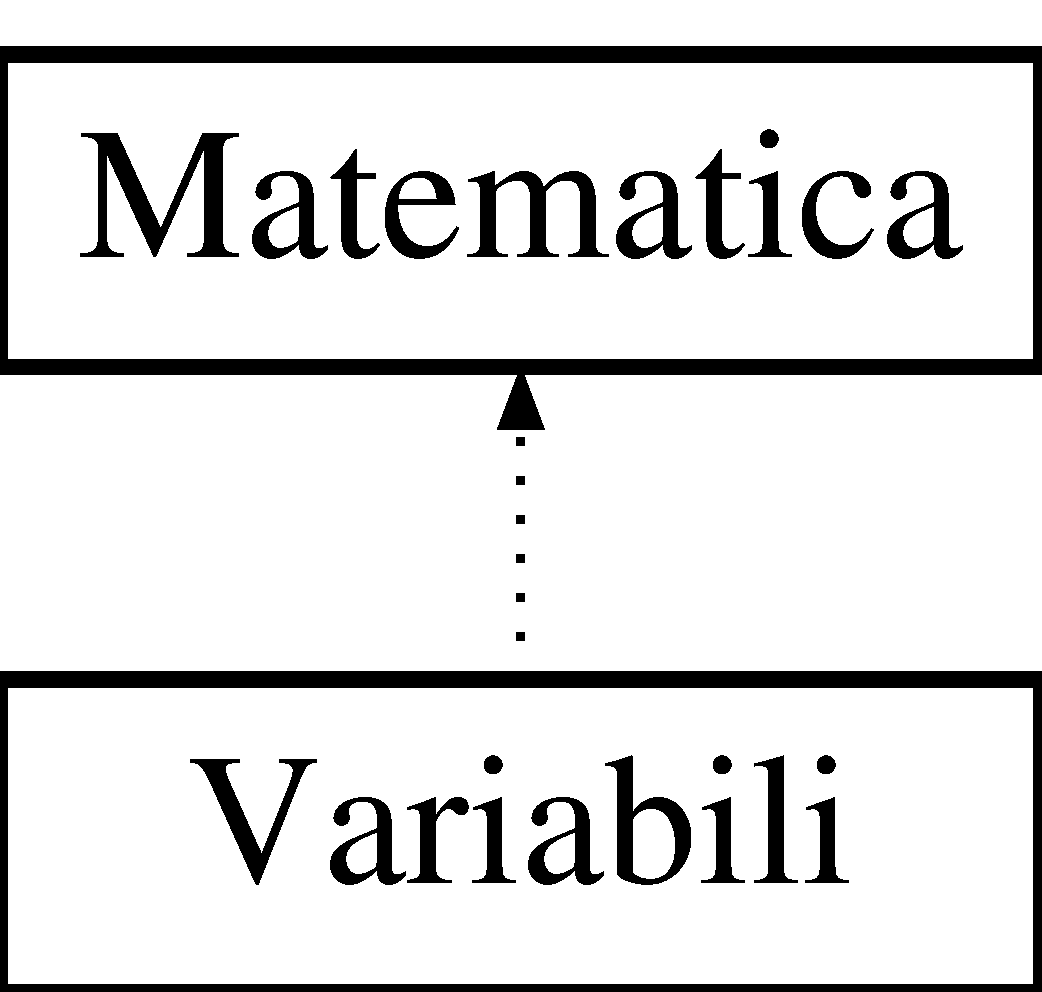
\includegraphics[height=2.000000cm]{classVariabili}
\end{center}
\end{figure}
\subsubsection*{\-Public \-Member \-Functions}
\begin{DoxyCompactItemize}
\item 
\hypertarget{classVariabili_af881fc3fcaf007a6ad92298c943be1e1}{{\bfseries \-Variabili} (int \-N\-Segn, int \-Potenza2, double \-Media\-Su, double \-Scarto\-Su, double \-Media\-Giu, double \-Scarto\-Giu, double \-Passo, double \-Incr)}\label{classVariabili_af881fc3fcaf007a6ad92298c943be1e1}

\item 
\hypertarget{classVariabili_a7d700d7f563966a19f9016ba03a9ff5c}{{\bfseries \-Variabili} (char $\ast$\-Nome\-Media, int \-Valori)}\label{classVariabili_a7d700d7f563966a19f9016ba03a9ff5c}

\item 
\hypertarget{classVariabili_aee1c6ef09b1a59200ab17589402e5813}{void {\bfseries \-Verificare} (int cosa, int \-Valore)}\label{classVariabili_aee1c6ef09b1a59200ab17589402e5813}

\item 
\hypertarget{classVariabili_a481b4c571a6e13c411f1564d1fa59322}{bool {\bfseries \-Simula} ()}\label{classVariabili_a481b4c571a6e13c411f1564d1fa59322}

\item 
\hypertarget{classVariabili_a0a9d83bb6daab4ecf2b7d88109cbf117}{bool {\bfseries \-Sifula} ()}\label{classVariabili_a0a9d83bb6daab4ecf2b7d88109cbf117}

\item 
\hypertarget{classVariabili_aa49dc238fd7a5356a4ff0f33505fd176}{void {\bfseries \-Scrivi\-File} ()}\label{classVariabili_aa49dc238fd7a5356a4ff0f33505fd176}

\item 
\hypertarget{classVariabili_a8966d84a169a5ae5f2fb4e4dff78d688}{void {\bfseries \-Cambia} (char $\ast$, int)}\label{classVariabili_a8966d84a169a5ae5f2fb4e4dff78d688}

\item 
\hypertarget{classVariabili_a2f097ce8803ddd5d4d36b59e6b8dbb37}{void {\bfseries \-Cambia} (char $\ast$, double)}\label{classVariabili_a2f097ce8803ddd5d4d36b59e6b8dbb37}

\end{DoxyCompactItemize}
\subsubsection*{\-Public \-Attributes}
\begin{DoxyCompactItemize}
\item 
\hypertarget{classVariabili_a252cfe0f42989230a3d7077400b5953f}{bool $\ast$ {\bfseries st}}\label{classVariabili_a252cfe0f42989230a3d7077400b5953f}

\item 
\hypertarget{classVariabili_ac2a9fda39fe1ec3fff7a0cc2b024e7a0}{double $\ast$ {\bfseries s\-Media}}\label{classVariabili_ac2a9fda39fe1ec3fff7a0cc2b024e7a0}

\item 
\hypertarget{classVariabili_aeb62e1458ef62b80a349f89b4d04d023}{int {\bfseries \-N\-Mass}}\label{classVariabili_aeb62e1458ef62b80a349f89b4d04d023}

\item 
\hypertarget{classVariabili_a78e1f6b081d4f4354ba9c3167a13f349}{int {\bfseries \-Periodi}}\label{classVariabili_a78e1f6b081d4f4354ba9c3167a13f349}

\item 
\hypertarget{classVariabili_ae17dca7f5e2139ba2ef487859c3f316e}{int {\bfseries \-N\-Segn}}\label{classVariabili_ae17dca7f5e2139ba2ef487859c3f316e}

\item 
\hypertarget{classVariabili_aba4c87cf3db463fff6b7a4518a16ee79}{double {\bfseries \-Media\-Su}}\label{classVariabili_aba4c87cf3db463fff6b7a4518a16ee79}

\item 
\hypertarget{classVariabili_ab2271c2915211972fca4cd75f6436b2d}{double {\bfseries \-Scarto\-Su}}\label{classVariabili_ab2271c2915211972fca4cd75f6436b2d}

\item 
\hypertarget{classVariabili_af164474f64237f66feda74e84081a644}{double {\bfseries \-Media\-Giu}}\label{classVariabili_af164474f64237f66feda74e84081a644}

\item 
\hypertarget{classVariabili_a9615e92bab38c7a4a2017a4d0a220606}{double {\bfseries \-Scarto\-Giu}}\label{classVariabili_a9615e92bab38c7a4a2017a4d0a220606}

\item 
\hypertarget{classVariabili_a048fe1e054cdfbf22b68f56840fd19fb}{double {\bfseries \-Passo}}\label{classVariabili_a048fe1e054cdfbf22b68f56840fd19fb}

\item 
\hypertarget{classVariabili_a891315d4365f283061bc7d4a1531df91}{double {\bfseries \-Incr}}\label{classVariabili_a891315d4365f283061bc7d4a1531df91}

\item 
\hypertarget{classVariabili_a9183b9e0d8b2ca559115ab7997093855}{\hyperlink{classMatematica}{\-Matematica} $\ast$ {\bfseries m\-Su}}\label{classVariabili_a9183b9e0d8b2ca559115ab7997093855}

\item 
\hypertarget{classVariabili_a2fbe4148b757ff50a40c170610e1fd94}{\hyperlink{classMatematica}{\-Matematica} $\ast$ {\bfseries m\-Giu}}\label{classVariabili_a2fbe4148b757ff50a40c170610e1fd94}

\end{DoxyCompactItemize}


\subsubsection{\-Detailed \-Description}


\-Definition at line 6 of file \-Var\-Segnali.\-h.



\-The documentation for this class was generated from the following files\-:\begin{DoxyCompactItemize}
\item 
src/\-Segnali/\-Var\-Segnali.\-h\item 
src/\-Segnali/\-Var\-Segnali.\-cpp\end{DoxyCompactItemize}

\hypertarget{structVERTEX}{}\subsection{V\+E\+R\+T\+EX Struct Reference}
\label{structVERTEX}\index{V\+E\+R\+T\+EX@{V\+E\+R\+T\+EX}}
\subsubsection*{Public Attributes}
\begin{DoxyCompactItemize}
\item 
double \hyperlink{structVERTEX_a863738e46f14b3bfc674ad87d35f143d}{Pos} \mbox{[}3\mbox{]}\hypertarget{structVERTEX_a863738e46f14b3bfc674ad87d35f143d}{}\label{structVERTEX_a863738e46f14b3bfc674ad87d35f143d}

\begin{DoxyCompactList}\small\item\em Vertex postion. \end{DoxyCompactList}\item 
int \hyperlink{structVERTEX_ac8859e8c1ce357c4c8b37bbb1936ba1c}{v}\hypertarget{structVERTEX_ac8859e8c1ce357c4c8b37bbb1936ba1c}{}\label{structVERTEX_ac8859e8c1ce357c4c8b37bbb1936ba1c}

\begin{DoxyCompactList}\small\item\em Vertex id. \end{DoxyCompactList}\item 
int \hyperlink{structVERTEX_ad82192d51ed2fc5973d034b41d0e4f27}{t} \mbox{[}M\+A\+X\+\_\+\+J\+O\+I\+N\+T\+\_\+\+V\+E\+R\+T\+EX\mbox{]}\hypertarget{structVERTEX_ad82192d51ed2fc5973d034b41d0e4f27}{}\label{structVERTEX_ad82192d51ed2fc5973d034b41d0e4f27}

\begin{DoxyCompactList}\small\item\em Triangles/lines connected (fixed size!!! should be enough) \end{DoxyCompactList}\item 
int \hyperlink{structVERTEX_a12a47df39f8f45d8c6da40a2238b1033}{N\+Tria}\hypertarget{structVERTEX_a12a47df39f8f45d8c6da40a2238b1033}{}\label{structVERTEX_a12a47df39f8f45d8c6da40a2238b1033}

\begin{DoxyCompactList}\small\item\em Number of triangles connected to the vertex. \end{DoxyCompactList}\end{DoxyCompactItemize}


\subsubsection{Detailed Description}


Definition at line 469 of file Cubo.\+h.



The documentation for this struct was generated from the following file\+:\begin{DoxyCompactItemize}
\item 
include/Cubo.\+h\end{DoxyCompactItemize}

\hypertarget{structVETT}{\subsection{\-V\-E\-T\-T \-Struct \-Reference}
\label{structVETT}\index{\-V\-E\-T\-T@{\-V\-E\-T\-T}}
}


\-Three dimentional vector.  




{\ttfamily \#include $<$\-Matematica\-Struct.\-h$>$}

\subsubsection*{\-Public \-Attributes}
\begin{DoxyCompactItemize}
\item 
\hypertarget{structVETT_a8639a6dd4fb3c4aa452b708733d827b4}{double \hyperlink{structVETT_a8639a6dd4fb3c4aa452b708733d827b4}{x} \mbox{[}3\mbox{]}}\label{structVETT_a8639a6dd4fb3c4aa452b708733d827b4}

\begin{DoxyCompactList}\small\item\em \-Position. \end{DoxyCompactList}\end{DoxyCompactItemize}


\subsubsection{\-Detailed \-Description}
\-Three dimentional vector. 

\-Definition at line 76 of file \-Matematica\-Struct.\-h.



\-The documentation for this struct was generated from the following file\-:\begin{DoxyCompactItemize}
\item 
include/\-Matematica\-Struct.\-h\end{DoxyCompactItemize}

\hypertarget{classVettore}{}\subsection{Vettore Class Reference}
\label{classVettore}\index{Vettore@{Vettore}}


Geometrical operations on vectors.  




{\ttfamily \#include $<$Matematica\+Vect.\+h$>$}

\subsubsection*{Public Member Functions}
\begin{DoxyCompactItemize}
\item 
\hyperlink{classVettore_a8be37a18dd9819f267ef0fca4770d6bf}{Vettore} (int N)\hypertarget{classVettore_a8be37a18dd9819f267ef0fca4770d6bf}{}\label{classVettore_a8be37a18dd9819f267ef0fca4770d6bf}

\begin{DoxyCompactList}\small\item\em Allocates. \end{DoxyCompactList}\item 
\hyperlink{classVettore_a8f9b4eac311cb366dd049eefa8d45d41}{Vettore} ()\hypertarget{classVettore_a8f9b4eac311cb366dd049eefa8d45d41}{}\label{classVettore_a8f9b4eac311cb366dd049eefa8d45d41}

\begin{DoxyCompactList}\small\item\em Allocates. \end{DoxyCompactList}\item 
\hyperlink{classVettore_a5864229515ff327ae85057b51a8035a6}{$\sim$\+Vettore} ()\hypertarget{classVettore_a5864229515ff327ae85057b51a8035a6}{}\label{classVettore_a5864229515ff327ae85057b51a8035a6}

\begin{DoxyCompactList}\small\item\em Frees. \end{DoxyCompactList}\item 
\hyperlink{classVettore_ab5b3efc833cf7efa62feeede44c377a5}{Vettore} (double $\ast$Pos, int N)\hypertarget{classVettore_ab5b3efc833cf7efa62feeede44c377a5}{}\label{classVettore_ab5b3efc833cf7efa62feeede44c377a5}

\begin{DoxyCompactList}\small\item\em Allocates and assigns. \end{DoxyCompactList}\item 
\hyperlink{classVettore_a4da1d1de9404fa6f377a45b6ddd36df8}{Vettore} (double \hyperlink{classVettore_a711aad4cbe735871dd9e91ab575c878b}{x}, double y, double z)\hypertarget{classVettore_a4da1d1de9404fa6f377a45b6ddd36df8}{}\label{classVettore_a4da1d1de9404fa6f377a45b6ddd36df8}

\begin{DoxyCompactList}\small\item\em Three dim vector. \end{DoxyCompactList}\item 
\hyperlink{classVettore_ad34a806257f874147444a9dad1d38b9c}{Vettore} (double \hyperlink{classVettore_a711aad4cbe735871dd9e91ab575c878b}{x}, double y)\hypertarget{classVettore_ad34a806257f874147444a9dad1d38b9c}{}\label{classVettore_ad34a806257f874147444a9dad1d38b9c}

\begin{DoxyCompactList}\small\item\em Two dim vector. \end{DoxyCompactList}\item 
double \hyperlink{classVettore_adbeac31b68a3e0dc78dfe0591d392e48}{Abs} ()\hypertarget{classVettore_adbeac31b68a3e0dc78dfe0591d392e48}{}\label{classVettore_adbeac31b68a3e0dc78dfe0591d392e48}

\begin{DoxyCompactList}\small\item\em Return the absolute value. \end{DoxyCompactList}\item 
double \hyperlink{classVettore_ac3486702edb3f0a9835908841db69cfd}{Norm} ()\hypertarget{classVettore_ac3486702edb3f0a9835908841db69cfd}{}\label{classVettore_ac3486702edb3f0a9835908841db69cfd}

\begin{DoxyCompactList}\small\item\em Return the norm of a \hyperlink{classVettore}{Vettore}. \end{DoxyCompactList}\item 
double \hyperlink{classVettore_aef629c102c4d237ef6e4897238f5bc18}{Normalize} ()\hypertarget{classVettore_aef629c102c4d237ef6e4897238f5bc18}{}\label{classVettore_aef629c102c4d237ef6e4897238f5bc18}

\begin{DoxyCompactList}\small\item\em Normlizes a \hyperlink{classVettore}{Vettore}. \end{DoxyCompactList}\item 
void \hyperlink{classVettore_a6c47c5bf64582210d56650fb8f490201}{Normal} (const \hyperlink{classVettore}{Vettore} $\ast$u, const \hyperlink{classVettore}{Vettore} $\ast$v)\hypertarget{classVettore_a6c47c5bf64582210d56650fb8f490201}{}\label{classVettore_a6c47c5bf64582210d56650fb8f490201}

\begin{DoxyCompactList}\small\item\em Computes the normal with respect to the \hyperlink{classVettore}{Vettore} u and v. \end{DoxyCompactList}\item 
void \hyperlink{classVettore_a37c16d330917daaf77a01df8d54d2ffa}{Normal\+Surf} (const \hyperlink{classVettore}{Vettore} $\ast$u, const \hyperlink{classVettore}{Vettore} $\ast$v, const \hyperlink{classVettore}{Vettore} $\ast$w)\hypertarget{classVettore_a37c16d330917daaf77a01df8d54d2ffa}{}\label{classVettore_a37c16d330917daaf77a01df8d54d2ffa}

\begin{DoxyCompactList}\small\item\em Computes the normal to the plane described by u,v,w. \end{DoxyCompactList}\item 
double \hyperlink{classVettore_a0076d507f0189c0bafa974af74afaae7}{Proj\+On\+Surf} (\hyperlink{classVettore}{Vettore} $\ast$S1, \hyperlink{classVettore}{Vettore} $\ast$S2, \hyperlink{classVettore}{Vettore} $\ast$S3, \hyperlink{classVettore}{Vettore} $\ast$P)\hypertarget{classVettore_a0076d507f0189c0bafa974af74afaae7}{}\label{classVettore_a0076d507f0189c0bafa974af74afaae7}

\begin{DoxyCompactList}\small\item\em Project a point P on the point PS perpendicular to the surface described by the points S1, S2 and S3. \end{DoxyCompactList}\item 
void \hyperlink{classVettore_a462cc9cf81c1f3a1b3c8b0136d6378d5}{Mult} (double Fact)\hypertarget{classVettore_a462cc9cf81c1f3a1b3c8b0136d6378d5}{}\label{classVettore_a462cc9cf81c1f3a1b3c8b0136d6378d5}

\begin{DoxyCompactList}\small\item\em multiply by a scalar \end{DoxyCompactList}\item 
void \hyperlink{classVettore_a5c3a30fe490ef9563842299380df3ba5}{Subs} (const \hyperlink{classVettore}{Vettore} $\ast$u, const \hyperlink{classVettore}{Vettore} $\ast$v)\hypertarget{classVettore_a5c3a30fe490ef9563842299380df3ba5}{}\label{classVettore_a5c3a30fe490ef9563842299380df3ba5}

\begin{DoxyCompactList}\small\item\em substruct two \hyperlink{classVettore}{Vettore} \end{DoxyCompactList}\item 
double \hyperlink{classVettore_a956dbbb6159671072b4eb5724b60748e}{ScalS} (const \hyperlink{classVettore}{Vettore} $\ast$u, const \hyperlink{classVettore}{Vettore} $\ast$v)\hypertarget{classVettore_a956dbbb6159671072b4eb5724b60748e}{}\label{classVettore_a956dbbb6159671072b4eb5724b60748e}

\begin{DoxyCompactList}\small\item\em Multiplies the components of a \hyperlink{classVettore}{Vettore} for a scalar. \end{DoxyCompactList}\item 
double \hyperlink{classVettore_a907339d7b281d6d87abaea47a47bcd25}{Cos\+Angle} (\hyperlink{classVettore}{Vettore} $\ast$u)
\begin{DoxyCompactList}\small\item\em Computes the cosine with respect to. \end{DoxyCompactList}\item 
double \hyperlink{classVettore_a72f38f80c8b2ea4b6dcd00d66ec24451}{Cos\+Angle} (\hyperlink{classVettore}{Vettore} $\ast$u, \hyperlink{classVettore}{Vettore} $\ast$v)\hypertarget{classVettore_a72f38f80c8b2ea4b6dcd00d66ec24451}{}\label{classVettore_a72f38f80c8b2ea4b6dcd00d66ec24451}

\begin{DoxyCompactList}\small\item\em Computes the cosine between two \hyperlink{classVettore}{Vettore}. \end{DoxyCompactList}\item 
double \hyperlink{classVettore_a8d84edbdf1f76b3065cc1c3291b98669}{Sin\+Angle} (\hyperlink{classVettore}{Vettore} $\ast$u, \hyperlink{classVettore}{Vettore} $\ast$v)\hypertarget{classVettore_a8d84edbdf1f76b3065cc1c3291b98669}{}\label{classVettore_a8d84edbdf1f76b3065cc1c3291b98669}

\begin{DoxyCompactList}\small\item\em Computes the sine between two \hyperlink{classVettore}{Vettore}. \end{DoxyCompactList}\item 
double \hyperlink{classVettore_a46f89489dcb6933de9154c63c82f8b61}{Sin\+Angle} (\hyperlink{classVettore}{Vettore} $\ast$u)
\begin{DoxyCompactList}\small\item\em Computes the sine with respect to. \end{DoxyCompactList}\item 
double \hyperlink{classVettore_a936e4b859237ce1643e932504dde2f22}{Angle} (\hyperlink{classVettore}{Vettore} $\ast$u, \hyperlink{classVettore}{Vettore} $\ast$v)\hypertarget{classVettore_a936e4b859237ce1643e932504dde2f22}{}\label{classVettore_a936e4b859237ce1643e932504dde2f22}

\begin{DoxyCompactList}\small\item\em Computes the angle between two Vetttore. \end{DoxyCompactList}\item 
double \hyperlink{classVettore_ac72b0f82d368ace2ef8090d276a9c751}{Angle} (\hyperlink{classVettore}{Vettore} $\ast$u)\hypertarget{classVettore_ac72b0f82d368ace2ef8090d276a9c751}{}\label{classVettore_ac72b0f82d368ace2ef8090d276a9c751}

\begin{DoxyCompactList}\small\item\em Computes the angle between two Vetttore. \end{DoxyCompactList}\item 
double \hyperlink{classVettore_ad018d767a0e0b15fbc17269db64d7574}{Col} (int N)\hypertarget{classVettore_ad018d767a0e0b15fbc17269db64d7574}{}\label{classVettore_ad018d767a0e0b15fbc17269db64d7574}

\begin{DoxyCompactList}\small\item\em Value of the N column. \end{DoxyCompactList}\item 
double \hyperlink{classVettore_a8fcbd69726df0d5309a4f2d790f427fd}{Val} (int N)\hypertarget{classVettore_a8fcbd69726df0d5309a4f2d790f427fd}{}\label{classVettore_a8fcbd69726df0d5309a4f2d790f427fd}

\begin{DoxyCompactList}\small\item\em Value of the N column. \end{DoxyCompactList}\item 
void \hyperlink{classVettore_af865716b201375aaca7c880377aa2426}{Set} (double \hyperlink{classVettore_a8fcbd69726df0d5309a4f2d790f427fd}{Val}, int \hyperlink{classVettore_ad018d767a0e0b15fbc17269db64d7574}{Col})\hypertarget{classVettore_af865716b201375aaca7c880377aa2426}{}\label{classVettore_af865716b201375aaca7c880377aa2426}

\begin{DoxyCompactList}\small\item\em Set the N column. \end{DoxyCompactList}\item 
void \hyperlink{classVettore_a5a767accac3ff301f062fce739190bb8}{Axis} (\hyperlink{classVettore}{Vettore} $\ast$u, \hyperlink{classVettore}{Vettore} $\ast$v)\hypertarget{classVettore_a5a767accac3ff301f062fce739190bb8}{}\label{classVettore_a5a767accac3ff301f062fce739190bb8}

\begin{DoxyCompactList}\small\item\em Calculates the axis formed by two \hyperlink{classVettore}{Vettore}. \end{DoxyCompactList}\item 
void \hyperlink{classVettore_acde6fcf2886d08085f11655e0bb4fa5a}{ScalV} (const \hyperlink{classVettore}{Vettore} $\ast$u, const \hyperlink{classVettore}{Vettore} $\ast$v)\hypertarget{classVettore_acde6fcf2886d08085f11655e0bb4fa5a}{}\label{classVettore_acde6fcf2886d08085f11655e0bb4fa5a}

\begin{DoxyCompactList}\small\item\em Scalar product between two \hyperlink{classVettore}{Vettore}. \end{DoxyCompactList}\item 
double \hyperlink{classVettore_a9b3422c7c865368c649cb008c6185250}{VetV} (const \hyperlink{classVettore}{Vettore} $\ast$u, const \hyperlink{classVettore}{Vettore} $\ast$v)\hypertarget{classVettore_a9b3422c7c865368c649cb008c6185250}{}\label{classVettore_a9b3422c7c865368c649cb008c6185250}

\begin{DoxyCompactList}\small\item\em Vectorial product between two \hyperlink{classVettore}{Vettore} returns the area. \end{DoxyCompactList}\item 
double \hyperlink{classVettore_a95399bdbce8cbb4ad68d53d914a68d76}{Vet\+V3} (const \hyperlink{classVettore}{Vettore} $\ast$u, const \hyperlink{classVettore}{Vettore} $\ast$v)\hypertarget{classVettore_a95399bdbce8cbb4ad68d53d914a68d76}{}\label{classVettore_a95399bdbce8cbb4ad68d53d914a68d76}

\begin{DoxyCompactList}\small\item\em Vectorial product between two \hyperlink{classVettore}{Vettore} in three dimension (faster) returns the area. \end{DoxyCompactList}\item 
double \hyperlink{classVettore_a23d7adb61da0e99cc2fab9dbab01f7d8}{VetV} (const \hyperlink{classVettore}{Vettore} $\ast$u)\hypertarget{classVettore_a23d7adb61da0e99cc2fab9dbab01f7d8}{}\label{classVettore_a23d7adb61da0e99cc2fab9dbab01f7d8}

\begin{DoxyCompactList}\small\item\em Vectorial product between two \hyperlink{classVettore}{Vettore} returns the area. \end{DoxyCompactList}\item 
double \hyperlink{classVettore_a060c730e982c30a0530598d864a6e508}{Proj\+On\+Axis} (\hyperlink{classVettore}{Vettore} $\ast$a)\hypertarget{classVettore_a060c730e982c30a0530598d864a6e508}{}\label{classVettore_a060c730e982c30a0530598d864a6e508}

\begin{DoxyCompactList}\small\item\em Projects along the axis. \end{DoxyCompactList}\item 
double \hyperlink{classVettore_a0521c48c381d2ddd16d4039c4d64a87b}{Proj\+On\+Axis} (\hyperlink{classVettore}{Vettore} $\ast$Pos, \hyperlink{classVettore}{Vettore} $\ast$\hyperlink{classVettore_a5a767accac3ff301f062fce739190bb8}{Axis})\hypertarget{classVettore_a0521c48c381d2ddd16d4039c4d64a87b}{}\label{classVettore_a0521c48c381d2ddd16d4039c4d64a87b}

\begin{DoxyCompactList}\small\item\em The length of Pos on Axis. \end{DoxyCompactList}\item 
void \hyperlink{classVettore_af4b317359ca70bbe6f41a178046d2e7f}{Apply\+On} (\hyperlink{classVettore}{Vettore} $\ast$o)\hypertarget{classVettore_af4b317359ca70bbe6f41a178046d2e7f}{}\label{classVettore_af4b317359ca70bbe6f41a178046d2e7f}

\begin{DoxyCompactList}\small\item\em Apply on a origin. \end{DoxyCompactList}\item 
void \hyperlink{classVettore_aed4e73920eb1f5d4d407c9913dd314f4}{Copy} (\hyperlink{classVettore}{Vettore} $\ast$o)\hypertarget{classVettore_aed4e73920eb1f5d4d407c9913dd314f4}{}\label{classVettore_aed4e73920eb1f5d4d407c9913dd314f4}

\begin{DoxyCompactList}\small\item\em Copy the vector. \end{DoxyCompactList}\item 
void \hyperlink{classVettore_a05beac72f2373cd7d3caa4ad8d3823be}{Export} (double $\ast$\hyperlink{classVettore_a711aad4cbe735871dd9e91ab575c878b}{x})\hypertarget{classVettore_a05beac72f2373cd7d3caa4ad8d3823be}{}\label{classVettore_a05beac72f2373cd7d3caa4ad8d3823be}

\begin{DoxyCompactList}\small\item\em Export. \end{DoxyCompactList}\item 
void \hyperlink{classVettore_ad289412e19e3a03ef86d329311712cff}{Perp\+To} (\hyperlink{classVettore}{Vettore} $\ast$o)\hypertarget{classVettore_ad289412e19e3a03ef86d329311712cff}{}\label{classVettore_ad289412e19e3a03ef86d329311712cff}

\begin{DoxyCompactList}\small\item\em The vector perpendicolar. \end{DoxyCompactList}\item 
double \hyperlink{classVettore_ab1ccf9725311b3fdb06d382bbdfc1066}{Perp\+To} (\hyperlink{classVettore}{Vettore} $\ast$Pos, \hyperlink{classVettore}{Vettore} $\ast$\hyperlink{classVettore_a5a767accac3ff301f062fce739190bb8}{Axis})\hypertarget{classVettore_ab1ccf9725311b3fdb06d382bbdfc1066}{}\label{classVettore_ab1ccf9725311b3fdb06d382bbdfc1066}

\begin{DoxyCompactList}\small\item\em The vector perpendicolar. \end{DoxyCompactList}\item 
double \hyperlink{classVettore_a0d1417eacc715d326e65e21a7c6d50ec}{Perp\+To3} (\hyperlink{classVettore}{Vettore} $\ast$Pos, \hyperlink{classVettore}{Vettore} $\ast$\hyperlink{classVettore_a5a767accac3ff301f062fce739190bb8}{Axis})\hypertarget{classVettore_a0d1417eacc715d326e65e21a7c6d50ec}{}\label{classVettore_a0d1417eacc715d326e65e21a7c6d50ec}

\begin{DoxyCompactList}\small\item\em The vector perpendicolar in three dimension (faster) \end{DoxyCompactList}\item 
void \hyperlink{classVettore_a9dcac18006ce057b8d78c847174c1362}{Print} ()\hypertarget{classVettore_a9dcac18006ce057b8d78c847174c1362}{}\label{classVettore_a9dcac18006ce057b8d78c847174c1362}

\begin{DoxyCompactList}\small\item\em Prints the components. \end{DoxyCompactList}\item 
void \hyperlink{classVettore_a735ba6810472f29b5158d6f266371c9b}{Rescale} (double New\+Length)\hypertarget{classVettore_a735ba6810472f29b5158d6f266371c9b}{}\label{classVettore_a735ba6810472f29b5158d6f266371c9b}

\begin{DoxyCompactList}\small\item\em Rescale the total length of the vector. \end{DoxyCompactList}\item 
\hyperlink{classVettore}{Vettore} \hyperlink{classVettore_aa47e7ac4476114c127060e8ab4b0bd1c}{operator+} (const \hyperlink{classVettore}{Vettore} \&Vet)\hypertarget{classVettore_aa47e7ac4476114c127060e8ab4b0bd1c}{}\label{classVettore_aa47e7ac4476114c127060e8ab4b0bd1c}

\begin{DoxyCompactList}\small\item\em Sum component by component. \end{DoxyCompactList}\item 
\hyperlink{classVettore}{Vettore} \hyperlink{classVettore_a90957078ca1e1545f53a7067cf712421}{operator+} (const \hyperlink{classVettore}{Vettore} \&Vet) const \hypertarget{classVettore_a90957078ca1e1545f53a7067cf712421}{}\label{classVettore_a90957078ca1e1545f53a7067cf712421}

\begin{DoxyCompactList}\small\item\em Sum component by component. \end{DoxyCompactList}\item 
\hyperlink{classVettore}{Vettore} \& \hyperlink{classVettore_a51ea7bee6d49e4b483dc91a38a6bcbe6}{operator+=} (const \hyperlink{classVettore}{Vettore} \&Vet)\hypertarget{classVettore_a51ea7bee6d49e4b483dc91a38a6bcbe6}{}\label{classVettore_a51ea7bee6d49e4b483dc91a38a6bcbe6}

\begin{DoxyCompactList}\small\item\em Sum component by component. \end{DoxyCompactList}\item 
\hyperlink{classVettore}{Vettore} \hyperlink{classVettore_a8a8192a424c70ae12496037159ef2294}{operator-\/} (const \hyperlink{classVettore}{Vettore} \&Vet)\hypertarget{classVettore_a8a8192a424c70ae12496037159ef2294}{}\label{classVettore_a8a8192a424c70ae12496037159ef2294}

\begin{DoxyCompactList}\small\item\em Difference component by component. \end{DoxyCompactList}\item 
\hyperlink{classVettore}{Vettore} \hyperlink{classVettore_a36b8a08fa27542f550b9b59d08fa4a45}{operator-\/} (const \hyperlink{classVettore}{Vettore} \&Vet) const \hypertarget{classVettore_a36b8a08fa27542f550b9b59d08fa4a45}{}\label{classVettore_a36b8a08fa27542f550b9b59d08fa4a45}

\begin{DoxyCompactList}\small\item\em Difference component by component. \end{DoxyCompactList}\item 
\hyperlink{classVettore}{Vettore} \& \hyperlink{classVettore_a3550f84cde64fde6694c6ecc67e08dae}{operator-\/=} (const \hyperlink{classVettore}{Vettore} \&Vet)\hypertarget{classVettore_a3550f84cde64fde6694c6ecc67e08dae}{}\label{classVettore_a3550f84cde64fde6694c6ecc67e08dae}

\begin{DoxyCompactList}\small\item\em Difference component by component. \end{DoxyCompactList}\item 
\hyperlink{classVettore}{Vettore} \hyperlink{classVettore_a00320cfea95d8047e4da795752c6fa86}{operator$\ast$} (const \hyperlink{classVettore}{Vettore} \&Vet)\hypertarget{classVettore_a00320cfea95d8047e4da795752c6fa86}{}\label{classVettore_a00320cfea95d8047e4da795752c6fa86}

\begin{DoxyCompactList}\small\item\em Moltiplication component by component. \end{DoxyCompactList}\item 
\hyperlink{classVettore}{Vettore} \& \hyperlink{classVettore_a77cef992de9faca80d4793e49fbca308}{operator$\ast$=} (const \hyperlink{classVettore}{Vettore} \&vec)\hypertarget{classVettore_a77cef992de9faca80d4793e49fbca308}{}\label{classVettore_a77cef992de9faca80d4793e49fbca308}

\begin{DoxyCompactList}\small\item\em Scalar product. \end{DoxyCompactList}\item 
\hyperlink{classVettore}{Vettore} \hyperlink{classVettore_abfb6a64e5e1a2d892a7ec95aeaf87a50}{operator$\ast$} (const double Fact)\hypertarget{classVettore_abfb6a64e5e1a2d892a7ec95aeaf87a50}{}\label{classVettore_abfb6a64e5e1a2d892a7ec95aeaf87a50}

\begin{DoxyCompactList}\small\item\em Moltiplication component by a scalar. \end{DoxyCompactList}\item 
\hyperlink{classVettore}{Vettore} \& \hyperlink{classVettore_a7f8dc90bb200d3eddb0e06df2bed55ac}{operator$\ast$=} (const double f)\hypertarget{classVettore_a7f8dc90bb200d3eddb0e06df2bed55ac}{}\label{classVettore_a7f8dc90bb200d3eddb0e06df2bed55ac}

\begin{DoxyCompactList}\small\item\em Moltiplication component by a scalar. \end{DoxyCompactList}\item 
double \hyperlink{classVettore_ac3246db90b8c4d550de3eab05f179509}{operator\%} (const \hyperlink{classVettore}{Vettore} \&Vet)\hypertarget{classVettore_ac3246db90b8c4d550de3eab05f179509}{}\label{classVettore_ac3246db90b8c4d550de3eab05f179509}

\begin{DoxyCompactList}\small\item\em Scalar product. \end{DoxyCompactList}\item 
double \& \hyperlink{classVettore_a478ce9f6aea546ba5e51de78f481e9a2}{operator\%=} (const \hyperlink{classVettore}{Vettore} \&Vet)\hypertarget{classVettore_a478ce9f6aea546ba5e51de78f481e9a2}{}\label{classVettore_a478ce9f6aea546ba5e51de78f481e9a2}

\begin{DoxyCompactList}\small\item\em Scalar product. \end{DoxyCompactList}\item 
\hyperlink{classVettore}{Vettore} \hyperlink{classVettore_a41cbdc407d57951a3a979cef317773e8}{operator$^\wedge$} (const \hyperlink{classVettore}{Vettore} \&vec)\hypertarget{classVettore_a41cbdc407d57951a3a979cef317773e8}{}\label{classVettore_a41cbdc407d57951a3a979cef317773e8}

\begin{DoxyCompactList}\small\item\em Vectorial product. \end{DoxyCompactList}\item 
\hyperlink{classVettore}{Vettore} \& \hyperlink{classVettore_a2680ccae9c643e24af0edacd4c1e6d46}{operator$^\wedge$=} (const \hyperlink{classVettore}{Vettore} \&vec)\hypertarget{classVettore_a2680ccae9c643e24af0edacd4c1e6d46}{}\label{classVettore_a2680ccae9c643e24af0edacd4c1e6d46}

\begin{DoxyCompactList}\small\item\em Vectorial product. \end{DoxyCompactList}\item 
\hyperlink{classVettore}{Vettore} \hyperlink{classVettore_aab8ad16c726ce7a08cfd9425aea42326}{operator/} (const \hyperlink{classVettore}{Vettore} \&vec)\hypertarget{classVettore_aab8ad16c726ce7a08cfd9425aea42326}{}\label{classVettore_aab8ad16c726ce7a08cfd9425aea42326}

\begin{DoxyCompactList}\small\item\em Division component by component. \end{DoxyCompactList}\item 
\hyperlink{classVettore}{Vettore} \& \hyperlink{classVettore_a21800796b8c71b2fbde47de0f4bca118}{operator/=} (const \hyperlink{classVettore}{Vettore} \&vec)\hypertarget{classVettore_a21800796b8c71b2fbde47de0f4bca118}{}\label{classVettore_a21800796b8c71b2fbde47de0f4bca118}

\begin{DoxyCompactList}\small\item\em Division component by component. \end{DoxyCompactList}\item 
\hyperlink{classVettore}{Vettore} \hyperlink{classVettore_ae984a878df7082f220fe8512856f843d}{operator=} (const \hyperlink{classVettore}{Vettore} \&Vet)\hypertarget{classVettore_ae984a878df7082f220fe8512856f843d}{}\label{classVettore_ae984a878df7082f220fe8512856f843d}

\begin{DoxyCompactList}\small\item\em Assigns the entries of the rhs \hyperlink{classVettore}{Vettore} to the lhs. \end{DoxyCompactList}\item 
double $\ast$ \hyperlink{classVettore_acde0dec95305cc462f912016373a77fe}{get\+Ptr} ()\hypertarget{classVettore_acde0dec95305cc462f912016373a77fe}{}\label{classVettore_acde0dec95305cc462f912016373a77fe}

\begin{DoxyCompactList}\small\item\em Returns a entry. \end{DoxyCompactList}\item 
const double $\ast$ \hyperlink{classVettore_ac9628a8286213402e12603779d7fe5ae}{get\+Ptr} () const \hypertarget{classVettore_ac9628a8286213402e12603779d7fe5ae}{}\label{classVettore_ac9628a8286213402e12603779d7fe5ae}

\begin{DoxyCompactList}\small\item\em Returns a entry. \end{DoxyCompactList}\item 
double \& \hyperlink{classVettore_a1928a371eb2c20841b3916ba9824b8a4}{operator\mbox{[}$\,$\mbox{]}} (int col)\hypertarget{classVettore_a1928a371eb2c20841b3916ba9824b8a4}{}\label{classVettore_a1928a371eb2c20841b3916ba9824b8a4}

\begin{DoxyCompactList}\small\item\em Returns a entry. \end{DoxyCompactList}\item 
double \hyperlink{classVettore_af57ef48295a3c4e8f3379287f2a7e687}{operator\mbox{[}$\,$\mbox{]}} (int col) const \hypertarget{classVettore_af57ef48295a3c4e8f3379287f2a7e687}{}\label{classVettore_af57ef48295a3c4e8f3379287f2a7e687}

\begin{DoxyCompactList}\small\item\em Returns a entry. \end{DoxyCompactList}\end{DoxyCompactItemize}
\subsubsection*{Public Attributes}
\begin{DoxyCompactItemize}
\item 
int \hyperlink{classVettore_a3b5e7568c0a268ec8bbeef7f29ea111a}{N\+Dim}\hypertarget{classVettore_a3b5e7568c0a268ec8bbeef7f29ea111a}{}\label{classVettore_a3b5e7568c0a268ec8bbeef7f29ea111a}

\begin{DoxyCompactList}\small\item\em Dimension allocated. \end{DoxyCompactList}\item 
double $\ast$ \hyperlink{classVettore_a711aad4cbe735871dd9e91ab575c878b}{x}\hypertarget{classVettore_a711aad4cbe735871dd9e91ab575c878b}{}\label{classVettore_a711aad4cbe735871dd9e91ab575c878b}

\begin{DoxyCompactList}\small\item\em Where the data are stored. \end{DoxyCompactList}\end{DoxyCompactItemize}


\subsubsection{Detailed Description}
Geometrical operations on vectors. 

Definition at line 9 of file Matematica\+Vect.\+h.



\subsubsection{Member Function Documentation}
\index{Vettore@{Vettore}!Cos\+Angle@{Cos\+Angle}}
\index{Cos\+Angle@{Cos\+Angle}!Vettore@{Vettore}}
\paragraph[{\texorpdfstring{Cos\+Angle(\+Vettore $\ast$u)}{CosAngle(Vettore *u)}}]{\setlength{\rightskip}{0pt plus 5cm}double Cos\+Angle (
\begin{DoxyParamCaption}
\item[{{\bf Vettore} $\ast$}]{u}
\end{DoxyParamCaption}
)}\hypertarget{classVettore_a907339d7b281d6d87abaea47a47bcd25}{}\label{classVettore_a907339d7b281d6d87abaea47a47bcd25}


Computes the cosine with respect to. 


\begin{DoxyParams}{Parameters}
{\em u} & \\
\hline
\end{DoxyParams}


Definition at line 229 of file Matematica\+Vect.\+cpp.



References N\+Dim, Norm(), and x.



Referenced by Angle(), Forces\+::\+Calc\+Bending(), and Proj\+On\+Axis().

\index{Vettore@{Vettore}!Sin\+Angle@{Sin\+Angle}}
\index{Sin\+Angle@{Sin\+Angle}!Vettore@{Vettore}}
\paragraph[{\texorpdfstring{Sin\+Angle(\+Vettore $\ast$u)}{SinAngle(Vettore *u)}}]{\setlength{\rightskip}{0pt plus 5cm}double Sin\+Angle (
\begin{DoxyParamCaption}
\item[{{\bf Vettore} $\ast$}]{u}
\end{DoxyParamCaption}
)}\hypertarget{classVettore_a46f89489dcb6933de9154c63c82f8b61}{}\label{classVettore_a46f89489dcb6933de9154c63c82f8b61}


Computes the sine with respect to. 


\begin{DoxyParams}{Parameters}
{\em u} & \\
\hline
\end{DoxyParams}


Definition at line 247 of file Matematica\+Vect.\+cpp.



References N\+Dim, Norm(), and x.



The documentation for this class was generated from the following files\+:\begin{DoxyCompactItemize}
\item 
include/Matematica\+Vect.\+h\item 
src/\+Matematica/Matematica\+Vect.\+cpp\end{DoxyCompactItemize}

\hypertarget{structXYZ}{\subsection{\-X\-Y\-Z \-Struct \-Reference}
\label{structXYZ}\index{\-X\-Y\-Z@{\-X\-Y\-Z}}
}


\-A \-Cartesian tern.  




{\ttfamily \#include $<$\-Var\-Data.\-h$>$}

\subsubsection*{\-Public \-Attributes}
\begin{DoxyCompactItemize}
\item 
\hypertarget{structXYZ_a8639a6dd4fb3c4aa452b708733d827b4}{double \hyperlink{structXYZ_a8639a6dd4fb3c4aa452b708733d827b4}{x} \mbox{[}3\mbox{]}}\label{structXYZ_a8639a6dd4fb3c4aa452b708733d827b4}

\begin{DoxyCompactList}\small\item\em \-Cartesian coordinates. \end{DoxyCompactList}\end{DoxyCompactItemize}


\subsubsection{\-Detailed \-Description}
\-A \-Cartesian tern. 

\-Definition at line 484 of file \-Var\-Data.\-h.



\-The documentation for this struct was generated from the following file\-:\begin{DoxyCompactItemize}
\item 
include/\-Var\-Data.\-h\end{DoxyCompactItemize}

\printindex
\end{document}
